\documentclass[11pt,a4paper,twoside]{article}
% The Book: the textbook edition of the coordination papers. Chapter order,
% numbering, parts, and edition metadata come from whitepaper/textbook.json;
% scripts/generate-mega-whitepaper.mjs renders the body, the front-matter map,
% the shared figures/pd-textbook-map.tex, and the single bibliography.
\newcommand{\pdgeneratedinput}[2]{%
  \IfFileExists{#1}{\input{#1}}{%
    \PackageError{coordination-papers-mega-volume}{Generated #2 is missing}{%
      From the repository root, run: node scripts/generate-mega-whitepaper.mjs
      .cache/whitepaper-build/coordination-papers-mega-volume}%
  }%
}
\usepackage{iftex}
\ifXeTeX\else
  \usepackage[utf8]{inputenc}
\fi
\usepackage[T1]{fontenc}
% Legacy text for maritime/technical; mathematical symbols for all editions.
% The shared typography module selects the Swiss sans after edition setup
% and guards against newpxtext's late reset of the body family.
\usepackage{newpxtext}
\usepackage{newpxmath}
% Monospace: TeX Gyre Cursor, the same family as Pagella, scaled to the
% text's lowercase.
% XeTeX computes a native word's height from glyph outlines by default; in
% this document that measurement comes back at about 2.4 em for many
% monospace words (whatever the font), which pushed every line carrying
% \texttt or \path down by a line and a half. With glyph metrics off the
% heights come from the fonts' ascent and descent, which fit the leading, and
% the interline spacing is uniform. Standalone chapters (pdfTeX) are unaffected.
\usepackage{iftex}
\ifXeTeX
  \XeTeXuseglyphmetrics=0
  \usepackage{fontspec}
  % Source Code Pro: dense, with a bold that separates typed input from output
  % in a session; sized to Palatino's lowercase. ItalicFont/BoldItalicFont are
  % declared because \lstdefinestyle{pdcode}'s commentstyle sets \itshape on
  % this family (see below) — without them fontspec has no `m/it` shape to
  % select and silently substitutes upright glyphs for every listing comment,
  % which is exactly the defect this comment used to leave unfixed.
  \setmonofont{SourceCodePro-Regular.otf}[BoldFont=SourceCodePro-Bold.otf,
    ItalicFont=SourceCodePro-RegularIt.otf,BoldItalicFont=SourceCodePro-BoldIt.otf,
    Scale=MatchLowercase]
  % Sans: TeX Gyre Heros, the grotesk the Swiss and technical editions already
  % use for display; without it \textsf falls to Latin Modern Sans.
  \setsansfont{texgyreheros-regular.otf}[ItalicFont=texgyreheros-italic.otf,
    BoldFont=texgyreheros-bold.otf,BoldItalicFont=texgyreheros-bolditalic.otf,
    Scale=MatchLowercase]
  % newpxmath declared its operators font and the \mathrm/\mathsf/\mathtt
  % alphabets before fontspec had set the faces, so every digit, \log, \max
  % and text subscript in math, and every pgfplots tick numeral, was set in
  % Latin Modern while the words around it were Palatino. The faces are
  % declared here under fixed NFSS family names and the math alphabets bound
  % to those names (the \rmdefault indirection resolved to Latin Modern).
  \newfontfamily\pdmathtextface{TeXGyrePagellaX-Regular.otf}[BoldFont=TeXGyrePagellaX-Bold.otf,
    ItalicFont=TeXGyrePagellaX-Italic.otf,BoldItalicFont=TeXGyrePagellaX-BoldItalic.otf,
    NFSSFamily=pdpag]
  \newfontfamily\pdmathsansface{texgyreheros-regular.otf}[BoldFont=texgyreheros-bold.otf,
    Scale=MatchLowercase,NFSSFamily=pdher]
  \newfontfamily\pdmathmonoface{SourceCodePro-Regular.otf}[BoldFont=SourceCodePro-Bold.otf,
    Scale=MatchLowercase,NFSSFamily=pdscp]
  \SetSymbolFont{operators}{normal}{TU}{pdpag}{m}{n}
  \SetSymbolFont{operators}{bold}{TU}{pdpag}{b}{n}
  \SetMathAlphabet{\mathrm}{normal}{TU}{pdpag}{m}{n}
  \SetMathAlphabet{\mathbf}{normal}{TU}{pdpag}{b}{n}
  \SetMathAlphabet{\mathit}{normal}{TU}{pdpag}{m}{it}
  \SetMathAlphabet{\mathsf}{normal}{TU}{pdher}{m}{n}
  \SetMathAlphabet{\mathtt}{normal}{TU}{pdscp}{m}{n}
  % The part openers set their display type in Times (the cover's face). Under
  % fontspec the legacy \fontfamily{ptm} has no TU italic or small caps, so the
  % face is declared here, with both.
  \newfontfamily\pdpartface{texgyretermes-regular.otf}[ItalicFont=texgyretermes-italic.otf,
    BoldFont=texgyretermes-bold.otf,BoldItalicFont=texgyretermes-bolditalic.otf,Ligatures=TeX]
  \newfontfamily\pdgrotesk{texgyreheros-regular.otf}[ItalicFont=texgyreheros-italic.otf,
    BoldFont=texgyreheros-bold.otf,BoldItalicFont=texgyreheros-bolditalic.otf,Ligatures=TeX]
  \newfontfamily\pdcovergrotesk{texgyreheros-regular.otf}[ItalicFont=texgyreheros-italic.otf,
    BoldFont=texgyreheros-bold.otf,BoldItalicFont=texgyreheros-bolditalic.otf,Ligatures=TeX,Kerning=On]
  \providecommand{\pdshorttitle}{The Harbor, the Person, and the Economy}
  % A 66-character column cannot hold a script path in one piece. Inside
  % \texttt, XeTeX's inter-character tokens allow a break (no hyphen) after
  % / _ . - = : and , so paths and flags wrap where a reader expects.
  \makeatletter
  \newXeTeXintercharclass\pd@brk
  \XeTeXcharclass`\/=\pd@brk \XeTeXcharclass`\_=\pd@brk \XeTeXcharclass`\.=\pd@brk
  \XeTeXcharclass`\-=\pd@brk \XeTeXcharclass`\==\pd@brk \XeTeXcharclass`\:=\pd@brk \XeTeXcharclass`\,=\pd@brk
  \XeTeXinterchartoks\pd@brk 0={\allowbreak}
  \XeTeXinterchartoks\pd@brk\pd@brk={\allowbreak}
  \expandafter\let\expandafter\pd@texttt\csname texttt \endcsname
  \expandafter\def\csname texttt \endcsname#1{{\XeTeXinterchartokenstate=1 \pd@texttt{#1}}}
  \makeatother
\else
  \newcommand\pdpartface{\fontfamily{ptm}\selectfont}
  \newcommand\pdgrotesk{\fontfamily{qhv}\selectfont}
  % pdfTeX fallback (not the published path; scripts/build-whitepapers.sh
  % compiles the Book with xelatex): the same face through its Type 1 package.
  \usepackage[scale=0.92]{sourcecodepro}
\fi
\let\openbox\relax
\usepackage[fontsize=10.5pt]{fontsize}
\usepackage{microtype}
\usepackage{geometry}
\usepackage{amsmath,amsthm}
\usepackage{listings}
\usepackage{xcolor}
\usepackage{booktabs}
\usepackage{tabularx}
\usepackage{xltabular}
\usepackage{array}
\usepackage{graphicx}
\usepackage{fancyhdr}
\usepackage{tikz}
\usepackage{float}
\usepackage{wrapfig}
% Page discipline for the Book. Every figure and table in the chapter sources
% asks for [H]; at a 7 x 10 trim that strands a third of a page whenever the
% next exhibit does not fit. In the Book an [H] becomes [!htbp]: the exhibit
% is still set here when it fits and otherwise floats to the top of the next
% page while the text flows on. Headings need room for three lines beneath them.
% Chapter boundaries already flush floats. Section barriers unnecessarily
% split short exhibits and their surrounding prose across nearly empty pages.
\usepackage{placeins}
\usepackage[skins,breakable]{tcolorbox}
\tcbuselibrary{listings}
\makeatletter
\let\pd@orig@xfloat\@xfloat
\def\@xfloat#1[#2]{\edef\@tempa{#2}\def\@tempb{H}%
  \ifx\@tempa\@tempb\pd@orig@xfloat#1[!htbp]\else\pd@orig@xfloat#1[#2]\fi}
% Float-only pages start at the text top, never vertically centred in a void.
\setlength{\@fptop}{0pt}
\setlength{\@fpsep}{16pt}
\makeatother
% A half-full figure must not eagerly consume a whole page while prose waits.
% Reserve float-only pages for substantial exhibits; ordinary diagrams share
% a page with text. Chapter/part boundaries still flush their own float queues.
\renewcommand{\floatpagefraction}{.8}
\renewcommand{\dblfloatpagefraction}{.8}
\renewcommand{\topfraction}{.85}
\renewcommand{\dbltopfraction}{.85}
\renewcommand{\textfraction}{.1}
% Keep at least two lines of a paragraph together across a page turn, and
% never split a hyphenated word between pages. Float reflow must not strand
% a run-in heading or a lone final syllable at the foot/head of adjacent pages.
\clubpenalty=10000
\widowpenalty=10000
\displaywidowpenalty=10000
\brokenpenalty=10000
\usepackage{needspace}
\usepackage{etoolbox}
% Breakable frames use \vsplit, whose retry loop cannot resolve an infinite
% penalty at the only usable split. Keep strong preferences inside frames,
% but allow the split; ordinary body paragraphs retain the strict rules above.
\AtBeginEnvironment{mdframed}{%
  \clubpenalty=9000 \widowpenalty=9000
  \displaywidowpenalty=9000 \brokenpenalty=9000}
% The reservation has to cover the heading's own apparatus before it covers any
% prose: a \section spends roughly 3.5 baselines on beforeskip, the heading line
% at \Large and afterskip, so 6 left about 2.5 lines of text under it -- right on
% the two-line rule page_spills enforces, and under it once the glue stretched.
% 5.5 (§5.5, The three subsystems of continuity) and 7.7.5 (Pricing the Bond) landed
% stranded that way in all three editions. 8 and 7 leave four clear lines, which
% is a margin rather than a coin flip, and holds for the Swiss and technical
% editions too, where Heros sets the heads larger than Pagella does.
\pretocmd{\section}{\Needspace*{8\baselineskip}}{}{}
\pretocmd{\subsection}{\Needspace*{7\baselineskip}}{}{}
\pretocmd{\subsubsection}{\Needspace*{7\baselineskip}}{}{}
\usepackage{caption}
\usepackage{enumitem}
\usepackage{refcount}
\usepackage{eso-pic}   % full-bleed jacket plate behind the title page
\usepackage[backref=page]{hyperref}
\usetikzlibrary{arrows.meta,positioning,fit,backgrounds,calc,shapes.geometric,shapes.symbols,decorations.pathmorphing,decorations.pathreplacing}
% Regime figures in the chapters (the sealed room's composition crossover and
% operating curve, and any later pgfplots fragment) need the axis environment
% in the Book as well as in the standalones.
\usepackage{pgfplots}
\pgfplotsset{compat=1.18}

% Trim 7 x 10 in (Wave 12, L1): one text column of 4.5 in (about 66 characters
% at 10.5 pt) and a 1.3 in outer margin column that carries sidenotes, margin
% heads, exercise pointers and margin figures. The standalone chapters keep A4.
% ---------------------------------------------------------------------------
% Editions. One set of chapter sources, three characters: maritime (the
% watercolour plates), swiss (colour blocking, grotesk display, flat marks) and
% technical (the Seventies manual: monoline ink, halftone, one warm accent,
% drawing-sheet openers). A driver root sets \pdedition before \input-ing the
% Book; without one, the Book takes the default set on the next line.
%
% Swiss is the central edition. The canonical artifact --
% coordination-papers-mega-volume.pdf, the file every published link on the
% site already points at -- renders Swiss because this default says so, which
% is the whole of the switch: no path, no link and no registry entry moves
% when the central edition changes, only this macro.
%
% Maritime and technical remain switchable and are NOT built for now. Their
% driver roots (coordination-papers-mega-volume-{maritime,technical}.tex),
% their plates and their branches in this preamble and in the root all stay in
% the tree, so either one still builds by hand:
%
%   scripts/build-whitepapers.sh coordination-papers-mega-volume-maritime
%
% They are simply out of the default build list in scripts/build-whitepapers.sh
% (see UNBUILT_EDITIONS there) and out of the published registry, because
% nothing publishes them today.
% ---------------------------------------------------------------------------
\providecommand{\pdedition}{swiss}
\newif\ifpdmaritime\newif\ifpdswiss\newif\ifpdtechnical
\makeatletter
\edef\pd@ed{\pdedition}
\def\pd@tmp{maritime}\ifx\pd@ed\pd@tmp\pdmaritimetrue\fi
\def\pd@tmp{swiss}\ifx\pd@ed\pd@tmp\pdswisstrue\fi
\def\pd@tmp{technical}\ifx\pd@ed\pd@tmp\pdtechnicaltrue\fi
\makeatother
% Shared Book typography. Suisse files stay outside the repository; the build
% supplies pd-book-font-config.tex through its private input directory. See
% fonts/README.md. An unlicensed checkout can only make an open-font proof.
\ifXeTeX\ifpdswiss
  \InputIfFileExists{pd-book-font-config.tex}{}{}
  \providecommand{\pdbookfontprofile}{open-proof}
  \ifdefstring{\pdbookfontprofile}{suisse}{%
    \ifdefined\pdbookfontdir\else
      \PackageError{pd-book-fonts}{Suisse requires a private font directory}{Run scripts/prepare-book-fonts.py with PD_BOOK_FONT_DIR set.}
    \fi
    \def\pdbookregular{SuisseIntl-Regular.otf}
    \def\pdbookbold{SuisseIntl-Semibold.otf}
    \def\pdbookitalic{SuisseIntl-RegularItalic.otf}
    \def\pdbookbolditalic{SuisseIntl-SemiboldItalic.otf}
    \def\pdbookdatafeatures{+tnum,+lnum}
    % These four purchased cuts have no small-cap glyph set. Legacy small-cap
    % requests retain the real upright face and current weight, never a fake
    % small-cap transform or an unrelated serif fallback.
    \renewcommand{\scshape}{\upshape}
    \typeout{BOOK FONT PROFILE: suisse (privately supplied, licensed files)}
  }{%
    \ifdefstring{\pdbookfontprofile}{open-proof}{}{%
      \PackageError{pd-book-fonts}{Unknown font profile}{Choose suisse or open-proof.}}
    \def\pdbookfontdir{fonts/source-sans/}
    \def\pdbookregular{SourceSans3-Regular.otf}
    \def\pdbookbold{SourceSans3-Semibold.otf}
    \def\pdbookitalic{SourceSans3-It.otf}
    \def\pdbookbolditalic{SourceSans3-SemiboldIt.otf}
    % Source Sans defaults to tabular lining numerals; it has no tnum feature.
    \def\pdbookdatafeatures{-pnum,-onum}
    \PackageWarningNoLine{pd-book-fonts}{OPEN-FONT PROOF: Source Sans 3, not Suisse. Page breaks and diagram clearance are not Suisse evidence}
  }
  \newcommand{\pdsetbookmainfont}{\setmainfont{\pdbookregular}[
    Path=\pdbookfontdir,Extension=.otf,
    BoldFont=\pdbookbold,ItalicFont=\pdbookitalic,
    BoldItalicFont=\pdbookbolditalic,Ligatures=TeX,Numbers=Proportional]}
  \pdsetbookmainfont
  % newpxtext selects Pagella in its earlier AtEndPreamble hook. Use the
  % public fontspec selector afterwards, so its NFSS and microtype state stay
  % coherent as well as the visible family. Merely changing rmdefault is not
  % enough: fontspec also maintains the small-cap and feature-bearing faces.
  \AtEndPreamble{\pdsetbookmainfont}
  \newfontfamily\pdtextface{\pdbookregular}[
    Path=\pdbookfontdir,Extension=.otf,
    BoldFont=\pdbookbold,ItalicFont=\pdbookitalic,
    BoldItalicFont=\pdbookbolditalic,Ligatures=TeX,
    Numbers=Proportional,NFSSFamily=pdbooktext]
  \let\pddisplayface\pdtextface
  \newfontfamily\pdcaptionface{\pdbookregular}[
    Path=\pdbookfontdir,Extension=.otf,
    BoldFont=\pdbookbold,ItalicFont=\pdbookitalic,
    BoldItalicFont=\pdbookbolditalic,Ligatures=TeX,
    RawFeature={\pdbookdatafeatures},NFSSFamily=pdbookdata]
  \setsansfont{\pdbookregular}[
    Path=\pdbookfontdir,Extension=.otf,
    BoldFont=\pdbookbold,ItalicFont=\pdbookitalic,
    BoldItalicFont=\pdbookbolditalic,Scale=MatchLowercase]
  \newfontfamily\pdinterfaceface{\pdbookregular}[
    Path=\pdbookfontdir,Extension=.otf,
    BoldFont=\pdbookbold,ItalicFont=\pdbookitalic,
    BoldItalicFont=\pdbookbolditalic,Scale=MatchLowercase,NFSSFamily=pdbookinterface]
  % Re-match the code face after setting the body face. Real italic and
  % semibold shapes are explicit throughout; no synthesized bold or slant.
  \setmonofont{SourceCodePro-Regular.otf}[BoldFont=SourceCodePro-Bold.otf,
    ItalicFont=SourceCodePro-RegularIt.otf,BoldItalicFont=SourceCodePro-BoldIt.otf,
    Scale=MatchLowercase]
  % Keep the proven newpx mathematical symbol/Greek fonts. Textual operators,
  % numerals, and explicit text alphabets match the sans prose. Replacing the
  % math engine is a separate, proof-sensitive change, not a font fallback.
  \SetSymbolFont{operators}{normal}{TU}{pdbookdata}{m}{n}
  \SetSymbolFont{operators}{bold}{TU}{pdbookdata}{b}{n}
  \SetMathAlphabet{\mathrm}{normal}{TU}{pdbooktext}{m}{n}
  \SetMathAlphabet{\mathbf}{normal}{TU}{pdbooktext}{b}{n}
  \SetMathAlphabet{\mathit}{normal}{TU}{pdbooktext}{m}{it}
  \SetMathAlphabet{\mathsf}{normal}{TU}{pdbookinterface}{m}{n}
  % Compatibility for existing shared headers. New work uses semantic roles.
  \renewcommand{\pdgrotesk}{\pdtextface}
  \renewcommand{\pdpartface}{\pddisplayface}
  % Captions often mix prose with taller mathematical symbols. Give that
  % combination real leading; changing face must not squeeze adjacent lines.
  \DeclareCaptionFont{pdbookcaption}{\pdcaptionface\linespread{1.16}\selectfont}
  \AtBeginDocument{%
    \hypersetup{pdfcreator={Book shared typography; font profile: \pdbookfontprofile}}%
    \captionsetup{font={small,pdbookcaption},labelfont=bf}%
    \renewcommand*{\marginfont}{\pdcaptionface\linespread{1.16}\footnotesize\raggedright\color{pdinkmuted}}}
\fi\fi
% Other editions retain their declared character, with the same role API.
\providecommand{\pdtextface}{\rmfamily}
\providecommand{\pddisplayface}{\pdgrotesk}
\providecommand{\pdcaptionface}{\rmfamily}
\providecommand{\pdinterfaceface}{\sffamily}

% The technical edition's accents are the brand's own Seventies trio: amber
% (mustard), rust (brown) and gold (avocado); no colour outside the palette.
\geometry{paperwidth=7in,paperheight=10in,inner=0.8in,outer=1.7in,%
  top=0.85in,bottom=0.95in,marginparsep=0.2in,marginparwidth=1.3in,headheight=14pt}
\normalmarginpar
% Preserve the authored vertical cadence. Flush-bottom composition stretches
% theorem and paragraph skips unpredictably on pages with fixed-height art.
\raggedbottom
\captionsetup{font=small,labelfont=bf}
\setlength{\emergencystretch}{3em}\tolerance=1500
% Contents includes every chapter, section and subsection. The single
% illustrated renderer below reads the live .toc; bookmarks retain their own
% depth. Figure and table lists keep the conventional locator treatment.
\setcounter{tocdepth}{2}
\makeatletter
\providecommand*{\toclevel@chapter}{0}
\renewcommand*\l@figure{\@dottedtocline{1}{1.2em}{2.8em}}
\renewcommand*\l@table{\@dottedtocline{1}{1.2em}{2.8em}}
\makeatother

\definecolor{codebg}{RGB}{248,248,248}
\definecolor{codeframe}{RGB}{200,200,200}
\definecolor{darkgreen}{HTML}{00564C}
\definecolor{darkblue}{HTML}{003FB8}
\definecolor{accent}{HTML}{00564C}
\definecolor{hhsand}{HTML}{E9DCC4}
\definecolor{hhsanddeep}{HTML}{D8C7A6}
\definecolor{hhebony}{HTML}{121212}
\definecolor{hhink}{HTML}{1B1712}
\definecolor{hhcobalt}{HTML}{003FB8}
\definecolor{hhamber}{HTML}{6B4500}
\definecolor{hhteal}{HTML}{00564C}
\definecolor{hhpaper}{HTML}{FBF7EF}
\definecolor{hhgray}{HTML}{5C5650}
% The Book's semantic color system: palette v2, light values. One hue, one meaning.
% Source of record for every hex: website-v2/src/styles/tokens.semantic.css (light
% theme); website-v2/scripts/check-figure-palette.mjs fails the build if this file
% and the tokens disagree. Twin copy under whitepaper/figures/ (byte-identical).
%
% Discipline: story colors are accents (rules, fills, marks, display text); body
% pages stay cream and ink. Amber is stripes, dots, and display only, never small
% text (3.71:1 on cream). Violet and gold are AA as text; use them at display size
% or on rules and fills. Line weights: 1px texture, 1.5px linework, 2px enclosure.
\definecolor{pdcobalt}{HTML}{003FB8}      % kernel / truth            --brand-primary
\definecolor{pdteal}{HTML}{006B5F}        % legibility                --brand-accent
\definecolor{pdhealth}{HTML}{1F7A4D}      % ready / coordinated       --story-health
\definecolor{pdindigo}{HTML}{353A85}      % protocol / federation     --story-indigo
\definecolor{pdviolet}{HTML}{933FA5}      % identity / continuity     --story-violet
\definecolor{pdrust}{HTML}{7A4514}        % reputation / trust earned --story-rust
\definecolor{pdgold}{HTML}{666A00}        % economy / value           --story-gold
\definecolor{pdslate}{HTML}{384856}       % foundation / bedrock      --story-slate
\definecolor{pderror}{HTML}{BF2F2F}       % breach / correction       --status-error
\definecolor{pdamber}{HTML}{A66F00}       % warning (display only)    --status-warning
\definecolor{pdlime}{HTML}{CAD900}        % highlight fill, ink text  --chart-yellow
\definecolor{pdink}{HTML}{121212}         % ink                       --text-primary
\definecolor{pdinkmuted}{HTML}{403B34}    % links, secondary text     --text-secondary
\definecolor{pdcream}{HTML}{F2EEE6}       % page ground               --surface-base
\definecolor{pdcreamraised}{HTML}{F7F3EB} % panels                    --surface-raised
\definecolor{pdcreamstrong}{HTML}{E9E2D5} % inset wells               --surface-strong
% Print inks for the Swiss edition of the Book (SWISS-BRIEF, B); print only.
\definecolor{pdswissblue}{HTML}{001489}
\definecolor{pdswissviolet}{HTML}{582C83}
\definecolor{pdswissred}{HTML}{DA291C}
% And the maritime edition's fourth ink: antique gold, the trim of the engraved
% plates carried onto the page (opener rules, part-title ornament, fillets round
% framed matter). Flat stand-in for a metallic pass; print only.
\definecolor{pdmaritimegold}{HTML}{805A14}

% GENERATED FILE. Do not edit by hand.
% Source of record: whitepaper/textbook.json (chapter order, numbers, parts, edition).
% Regenerate both committed copies: node scripts/generate-mega-whitepaper.mjs --sync-shared
% Drift check (CI): node --test scripts/generate-mega-whitepaper.test.mjs
% Twin copies: whitepaper/figures/pd-textbook-map.tex and
%              website-v2/public/whitepaper/figures/pd-textbook-map.tex (byte-identical).
%
% Every standalone chapter preamble defines \pdchapterprefix before inputting
% this file; the Book redefines it at every \pdchapter. Everything else derives.

\providecommand{\pdeditiontitle}{Governing AI Agents: The Harbor, the Person, and the Economy}
\providecommand{\pdeditionsubtitle}{A Textbook of Concurrency, Identity, and Accountable Autonomous Work}
\providecommand{\pdeditionversion}{4.0 (Textbook Edition)}
\providecommand{\pdeditiondate}{September 2026}
\providecommand{\pdeditionclaim}{For autonomous work to remain accountable, each action needs an authority, a record, and someone responsible for its consequences.}
\providecommand{\pdbooktitle}{\emph{\pdeditiontitle}}
\providecommand{\pdchaptercount}{8}
\providecommand{\pdchaptercountword}{eight}
\providecommand{\pdpartcount}{4}
\providecommand{\pdchapterprefix}{none}
\expandafter\providecommand\csname pdchapternumberofnone\endcsname{0}
\expandafter\providecommand\csname pdchaptertitleofnone\endcsname{\pdeditiontitle}
\expandafter\providecommand\csname pdchaptercolorofnone\endcsname{pdcobalt}
\expandafter\providecommand\csname pdchapternumberofswk\endcsname{1}
\expandafter\providecommand\csname pdchaptertitleofswk\endcsname{The Single-Writer Kernel}
\expandafter\providecommand\csname pdchaptercolorofswk\endcsname{pdcobalt}
\expandafter\providecommand\csname pdchapterformerofswk\endcsname{II}
\expandafter\providecommand\csname pdchapterpartindexofswk\endcsname{1}
\expandafter\providecommand\csname pdchapterpartlabelofswk\endcsname{Part I \textperiodcentered\ Ground Truth}
\expandafter\providecommand\csname pdchapterquestionofswk\endcsname{Where can a rule be made real?}
\expandafter\providecommand\csname pdchapteronelineofswk\endcsname{One writer orders changes to a local database; the chapter specifies which failures that record can survive.}
\expandafter\providecommand\csname pdchapterepigraphofswk\endcsname{There is no fundamental need to keep a database at all; the log is all the information there is. The only reason for storing the database is performance of retrieval operations.}
\expandafter\providecommand\csname pdchapterepigraphsourceofswk\endcsname{Jim Gray and Andreas Reuter, Transaction Processing: Concepts and Techniques, 1993}
\expandafter\providecommand\csname pdchapternumberofanchor\endcsname{2}
\expandafter\providecommand\csname pdchaptertitleofanchor\endcsname{The Anchor Protocol}
\expandafter\providecommand\csname pdchaptercolorofanchor\endcsname{pdcobalt}
\expandafter\providecommand\csname pdchapterformerofanchor\endcsname{V}
\expandafter\providecommand\csname pdchapterpartindexofanchor\endcsname{1}
\expandafter\providecommand\csname pdchapterpartlabelofanchor\endcsname{Part I \textperiodcentered\ Ground Truth}
\expandafter\providecommand\csname pdchapterquestionofanchor\endcsname{How may authority travel without silently growing?}
\expandafter\providecommand\csname pdchapteronelineofanchor\endcsname{Delegated capability only narrows: every child is a subset of its parent, at every hop, and the verifier checks the whole chain.}
\expandafter\providecommand\csname pdchapterepigraphofanchor\endcsname{Every program and every user of the system should operate using the least set of privileges necessary to complete the job.}
\expandafter\providecommand\csname pdchapterepigraphsourceofanchor\endcsname{Jerome Saltzer and Michael Schroeder, The Protection of Information in Computer Systems, 1975}
\expandafter\providecommand\csname pdchapternumberofsealed\endcsname{3}
\expandafter\providecommand\csname pdchaptertitleofsealed\endcsname{The Sealed Harbor}
\expandafter\providecommand\csname pdchaptercolorofsealed\endcsname{pdcobalt}
\expandafter\providecommand\csname pdchapterformerofsealed\endcsname{}
\expandafter\providecommand\csname pdchapterpartindexofsealed\endcsname{1}
\expandafter\providecommand\csname pdchapterpartlabelofsealed\endcsname{Part I \textperiodcentered\ Ground Truth}
\expandafter\providecommand\csname pdchapterquestionofsealed\endcsname{What can a sealed agent leak, and how would we know?}
\expandafter\providecommand\csname pdchapteronelineofsealed\endcsname{A confined work order has explicit release gates and a shared leakage budget, under the model's stated channel assumptions.}
\expandafter\providecommand\csname pdchapterepigraphofsealed\endcsname{This note explores the problem of confining a program during its execution so that it cannot transmit information to any other program except its caller.}
\expandafter\providecommand\csname pdchapterepigraphsourceofsealed\endcsname{Butler W. Lampson, A Note on the Confinement Problem, 1973}
\expandafter\providecommand\csname pdchapternumberofls\endcsname{4}
\expandafter\providecommand\csname pdchaptertitleofls\endcsname{The Legible Swarm}
\expandafter\providecommand\csname pdchaptercolorofls\endcsname{pdteal}
\expandafter\providecommand\csname pdchapterformerofls\endcsname{I}
\expandafter\providecommand\csname pdchapterpartindexofls\endcsname{2}
\expandafter\providecommand\csname pdchapterpartlabelofls\endcsname{Part II \textperiodcentered\ The Cost of Seeing}
\expandafter\providecommand\csname pdchapterquestionofls\endcsname{What must remain visible, and what does seeing cost?}
\expandafter\providecommand\csname pdchapteronelineofls\endcsname{Useful supervision requires summaries that preserve the operator's decisions and link back to inspectable evidence.}
\expandafter\providecommand\csname pdchapterepigraphofls\endcsname{In an information-rich world, the wealth of information means a dearth of something else: a scarcity of whatever it is that information consumes. What information consumes is rather obvious: it consumes the attention of its recipients.}
\expandafter\providecommand\csname pdchapterepigraphsourceofls\endcsname{Herbert A. Simon, Designing Organizations for an Information-Rich World, 1971}
\expandafter\providecommand\csname pdchapternumberofstp\endcsname{5}
\expandafter\providecommand\csname pdchaptertitleofstp\endcsname{From Spawn to Person}
\expandafter\providecommand\csname pdchaptercolorofstp\endcsname{pdviolet}
\expandafter\providecommand\csname pdchapterformerofstp\endcsname{III}
\expandafter\providecommand\csname pdchapterpartindexofstp\endcsname{3}
\expandafter\providecommand\csname pdchapterpartlabelofstp\endcsname{Part III \textperiodcentered\ What Survives the Restart}
\expandafter\providecommand\csname pdchapterquestionofstp\endcsname{What remains long enough to owe anything?}
\expandafter\providecommand\csname pdchapteronelineofstp\endcsname{Continuity turns an anonymous spawn into a ledger position with a witnessed record; reputation is what that record is worth.}
\expandafter\providecommand\csname pdchapterepigraphofstp\endcsname{We are but whirlpools in a river of ever-flowing water. We are not stuff that abides, but patterns that perpetuate themselves.}
\expandafter\providecommand\csname pdchapterepigraphsourceofstp\endcsname{Norbert Wiener, The Human Use of Human Beings: Cybernetics and Society, 1950}
\expandafter\providecommand\csname pdchapternumberofhe\endcsname{6}
\expandafter\providecommand\csname pdchaptertitleofhe\endcsname{The Harbor Economy}
\expandafter\providecommand\csname pdchaptercolorofhe\endcsname{pdgold}
\expandafter\providecommand\csname pdchapterformerofhe\endcsname{IV}
\expandafter\providecommand\csname pdchapterpartindexofhe\endcsname{4}
\expandafter\providecommand\csname pdchapterpartlabelofhe\endcsname{Part IV \textperiodcentered\ Trade Between Strangers}
\expandafter\providecommand\csname pdchapterquestionofhe\endcsname{What makes cooperation rational without making loss unbounded?}
\expandafter\providecommand\csname pdchapteronelineofhe\endcsname{Labor, rented assets, and licensed skills expose different risks but settle through a shared ledger that conserves each native unit.}
\expandafter\providecommand\csname pdchapterepigraphofhe\endcsname{The main reason why it is profitable to establish a firm would seem to be that there is a cost of using the price mechanism.}
\expandafter\providecommand\csname pdchapterepigraphsourceofhe\endcsname{Ronald H. Coase, The Nature of the Firm, 1937}
\expandafter\providecommand\csname pdchapternumberofbonded\endcsname{7}
\expandafter\providecommand\csname pdchaptertitleofbonded\endcsname{The Bonded Commons}
\expandafter\providecommand\csname pdchaptercolorofbonded\endcsname{pdgold}
\expandafter\providecommand\csname pdchapterformerofbonded\endcsname{VI}
\expandafter\providecommand\csname pdchapterpartindexofbonded\endcsname{4}
\expandafter\providecommand\csname pdchapterpartlabelofbonded\endcsname{Part IV \textperiodcentered\ Trade Between Strangers}
\expandafter\providecommand\csname pdchapterquestionofbonded\endcsname{Who may decide, on what evidence, with what consequence?}
\expandafter\providecommand\csname pdchapteronelineofbonded\endcsname{Bonds, witnesses, audits and appeals turn residual uncertainty into an institution; the ledger's conservation law is mechanically checked.}
\expandafter\providecommand\csname pdchapterepigraphofbonded\endcsname{The power to constrain an adversary may depend on the power to bind oneself.}
\expandafter\providecommand\csname pdchapterepigraphsourceofbonded\endcsname{Thomas C. Schelling, The Strategy of Conflict, 1960}
\expandafter\providecommand\csname pdchapternumberoffh\endcsname{8}
\expandafter\providecommand\csname pdchaptertitleoffh\endcsname{The Federated Harbor}
\expandafter\providecommand\csname pdchaptercoloroffh\endcsname{pdgold}
\expandafter\providecommand\csname pdchapterformeroffh\endcsname{VII}
\expandafter\providecommand\csname pdchapterpartindexoffh\endcsname{4}
\expandafter\providecommand\csname pdchapterpartlabeloffh\endcsname{Part IV \textperiodcentered\ Trade Between Strangers}
\expandafter\providecommand\csname pdchapterquestionoffh\endcsname{What can cross a trust boundary without moving the authority itself?}
\expandafter\providecommand\csname pdchapteronelineoffh\endcsname{Mutually distrustful machines relay evidence, not sovereignty: what may gossip, what needs an authority point, and how a grant crosses a boundary.}
\expandafter\providecommand\csname pdchapterepigraphoffh\endcsname{We reject: kings, presidents and voting. We believe in: rough consensus and running code.}
\expandafter\providecommand\csname pdchapterepigraphsourceoffh\endcsname{David D. Clark, A Cloudy Crystal Ball: Visions of the Future, 1992}
\providecommand{\pdchapternumber}{\csname pdchapternumberof\pdchapterprefix\endcsname}
\providecommand{\pdchaptertitle}{\csname pdchaptertitleof\pdchapterprefix\endcsname}
\providecommand{\pdchaptercolor}{\csname pdchaptercolorof\pdchapterprefix\endcsname}
\providecommand{\pdchapterpartindex}{\csname pdchapterpartindexof\pdchapterprefix\endcsname}
\providecommand{\pdchapterpartlabel}{\csname pdchapterpartlabelof\pdchapterprefix\endcsname}
\providecommand{\pdchapterquestion}{\csname pdchapterquestionof\pdchapterprefix\endcsname}
\providecommand{\pdchapteroneline}{\csname pdchapteronelineof\pdchapterprefix\endcsname}
\providecommand{\pdchapterepigraph}{\csname pdchapterepigraphof\pdchapterprefix\endcsname}
\providecommand{\pdchapterepigraphsource}{\csname pdchapterepigraphsourceof\pdchapterprefix\endcsname}

% Parts, for the weighted four-hue rule: numeral, hue, the label that ends the
% part (the next part, or the appendices), and the chapter count used as the
% weight until page references exist. \pdweightrule (Book preamble) consumes it.
\providecommand{\pdfirstpartnumeral}{I}
\providecommand{\pdweightsegmentslist}{%
  \pdweightsegment{I}{pdcobalt}{part:II}{3}%
  \pdweightsegment{II}{pdteal}{part:III}{1}%
  \pdweightsegment{III}{pdviolet}{part:IV}{1}%
  \pdweightsegment{IV}{pdgold}{book:appendices}{3}%
}
\expandafter\providecommand\csname pdpartindexofI\endcsname{1}
\expandafter\providecommand\csname pdpartindexofII\endcsname{2}
\expandafter\providecommand\csname pdpartindexofIII\endcsname{3}
\expandafter\providecommand\csname pdpartindexofIV\endcsname{4}
\expandafter\providecommand\csname pdparttitleofI\endcsname{Ground Truth}
\expandafter\providecommand\csname pdparttitleofII\endcsname{The Cost of Seeing}
\expandafter\providecommand\csname pdparttitleofIII\endcsname{What Survives the Restart}
\expandafter\providecommand\csname pdparttitleofIV\endcsname{Trade Between Strangers}

% Locator map: every part and chapter of the Book, the current chapter marked.
% \pdchaplink is provided by figures/pd-hyperlinks.tex (a live link inside the
% Book, plain text in a standalone chapter).
\providecommand{\pdmapchapter}[3]{%
  \ifnum#1=\pdchapternumber\relax
    \textbf{\pdchaplink{#2}{#1.~#3}}~\textnormal{(this chapter)}%
  \else
    \pdchaplink{#2}{#1.~#3}%
  \fi}
\providecommand{\pdtextbookmap}{%
  \begin{tabular}{@{}l@{\quad}p{\dimexpr\linewidth-12em\relax}@{}}
  \textsc{\textbf{Part I}}\ Ground Truth & \raggedright \pdmapchapter{1}{swk}{The Single-Writer Kernel} \textperiodcentered\ \pdmapchapter{2}{anchor}{The Anchor Protocol} \textperiodcentered\ \pdmapchapter{3}{sealed}{The Sealed Harbor}\tabularnewline[2pt]
  \textsc{\textbf{Part II}}\ The Cost of Seeing & \raggedright \pdmapchapter{4}{ls}{The Legible Swarm}\tabularnewline[2pt]
  \textsc{\textbf{Part III}}\ What Survives the Restart & \raggedright \pdmapchapter{5}{stp}{From Spawn to Person}\tabularnewline[2pt]
  \textsc{\textbf{Part IV}}\ Trade Between Strangers & \raggedright \pdmapchapter{6}{he}{The Harbor Economy} \textperiodcentered\ \pdmapchapter{7}{bonded}{The Bonded Commons} \textperiodcentered\ \pdmapchapter{8}{fh}{The Federated Harbor}\tabularnewline[2pt]
  \end{tabular}}

% Shared pedagogic apparatus for the Book and every standalone chapter: boxed
% claims, honest boundaries, worked examples, retrieval prompts, numbered
% exercises, and their deferred solutions.
% Twin copy under whitepaper/figures/ (byte-identical; checked by
% scripts/generate-mega-whitepaper.test.mjs).
%
% \input this immediately after figures/pd-textbook-map (so \pdchapterprefix
% and \pdchapternumber already resolve) and before figures/pd-hyperlinks.
%
% Page grammar (Wave 12): a content kind is signalled by typography and the
% margin, never by a tinted rectangle. Claims: a hairline above, a small-caps
% run-in head, a short hairline below. Worked examples: two hairlines and an
% italic head. Boundaries: a plain ink bar at the left, no fill. Recitation:
% margin prompts in the Book, a compact list in a standalone chapter.
% Exercises: a numbered hanging paragraph with kind and stars in small caps,
% the solution page in the margin. Nothing here paints a background.
%
% \ifpdmargincolumn is false by default (standalone A4 chapters have no margin
% column); the Book's preamble sets \pdmargincolumntrue after its geometry.
% mdframed is used only for the bars (leftline) and hairlines (top/bottom),
% with the DEFAULT frame method -- never framemethod=tikz.
%
% Key-value parsing for \pdexercise uses pgfkeys: pgf ships as part of tikz,
% which every preamble already loads, so this adds no new dependency (keyval
% would have meant one). The closed kind/rating vocabularies are enforced with
% the LaTeX kernel's own \in@/\ifin@ comma-list test -- always available,
% no package of its own -- wrapped in an \edef that expands both sides first:
% \in@ does not expand its own arguments, so hunting for a *macro* (rather
% than literal text) requires pre-expanding it, or every kind reads as absent.
\makeatletter
\@ifpackageloaded{mdframed}{}{\usepackage{mdframed}}
\@ifpackageloaded{answers}{}{\usepackage{answers}}
\@ifpackageloaded{marginnote}{}{\usepackage{marginnote}}
\@ifpackageloaded{environ}{}{\usepackage{environ}}
\@ifpackageloaded{etoolbox}{}{\usepackage{etoolbox}}
\@ifpackageloaded{listings}{}{\usepackage{listings}}
\@ifpackageloaded{caption}{}{\usepackage{caption}}
\@ifpackageloaded{tcolorbox}{}{\usepackage[skins,breakable,listings]{tcolorbox}}

% ---------------------------------------------------------------------------
% Shared helpers: the margin-column switch, the margin head, the margin glyph.
% ---------------------------------------------------------------------------
% The Book defines \pdcurrentchaptercolor (per part) AFTER this file; a
% standalone chapter never does. Resolve it lazily, falling back to cobalt.
\newcommand{\pd@chaptercolor}{\ifdefined\pdcurrentchaptercolor\pdcurrentchaptercolor\else pdcobalt\fi}
% The eight standalone chapter PDFs this false branch exists for are retired
% as of this change (the chapters no longer build or publish an A4 edition of
% themselves). Every \ifpdmargincolumn false branch below is now dead weight
% kept alive only by the chapters' .tex sources still being independently
% compilable; do NOT delete it in this change -- the margin apparatus work is
% in flight on another branch and this would collide with it. Removing the
% false branch (and, eventually, the conditional itself) is that wave's job.
\newif\ifpdmargincolumn
\pdmargincolumnfalse
% The Book overrides this with an unnumbered, baseline-aligned margin aside.
% Keep chapter sources independently compilable without duplicating prose.
\providecommand{\pdsourceaside}[1]{\footnote{#1}}
% An intentional body boundary: flush pending figures before a new margin
% discussion. The generator strips legacy literal chapter-opening breaks,
% but preserves this explicit editorial instruction. Never use it in frames.
\newcommand{\pdmarginpagebreak}{\clearpage}
\renewcommand*{\marginfont}{\footnotesize\raggedright\color{pdinkmuted}}
% A small-caps head: set in the margin when the Book has a margin column,
% otherwise run in at the start of the paragraph.
% A head stays a \marginnote, and the reason is worth keeping. It was set as
% a \marginpar for one build (2026-09-08), so the page builder would keep the
% Recall block clear of it, and the build died with "Float(s) lost" at the end
% of chapter 1. \ifinner is true inside a minipage or mdframed only BETWEEN
% paragraphs; the moment a paragraph starts it is ordinary horizontal mode,
% \ifinner is false, and a \marginpar issued there -- a \keyidea inside a
% pdexample -- has no page to be shipped to. The heads are one line each and
% are never what runs into something; the Recall block was, and it is now a
% \marginpar issued in vertical mode, where the test is honest.
% Each head records the page and the page-height at which it was issued, so a
% Recall block raised later on the same page can stop short of it. A head is
% issued at the start of its paragraph, where \pagetotal is the page above the
% paragraph -- the head's own position, to within a line.
% Margin occupancy is tracked both ways. A head records where it was issued
% so a Recall block raised later on the page stops short of it; a Recall block
% records where its foot came to rest so a head issued later on the same page
% (the next section's first Key idea) steps down below it instead of printing
% inside it. \pagetotal at a head lags by the current paragraph, which puts
% every error on the safe side: the block is capped a little low, the head
% steps a little far.
\def\pd@lastheadpage{0}\newlength{\pd@lastheadbottom}
\def\pd@blockpage{0}\newlength{\pd@blockbottom}\newlength{\pd@headshift}
\newsavebox{\pd@headbox}\newsavebox{\pd@ptrbox}\newsavebox{\pd@sidebox}
% Run the page builder so \pagetotal counts the paragraph that just ended.
% Without it \pagetotal is the page above the LAST paragraph the builder saw,
% which under-reads by however much prose has since been set -- and every
% device here decides where it may sit from that number. A Boundary head read
% a stale \pagetotal and recorded its foot a paragraph too high, and the Recall
% block that followed cleared that phantom and printed on the head itself
% (0.1 pt apart on p. 253 of the technical edition). \penalty\@M contributes
% without opening a breakpoint. Outer vertical mode only: inside a box the
% penalty lands on the box's own list and settles nothing.
\newcommand{\pd@settle}{\ifvmode\ifinner\else\penalty\@M\vskip\z@\fi\fi}
% ---------------------------------------------------------------------------
% Figure-band tracking, for vertical CENTERING of a margin device against the
% main-column figure it accompanies (2026-09). \pd@figtop/\pd@figbot/\pd@figpage
% are declared here but SET in the Book preamble's \pgfsys@typesetpicturebox
% hook (coordination-papers-mega-volume-preamble.tex), not by an
% \AtBeginEnvironment{figure}/\AtEndEnvironment{figure} pair on \pagetotal --
% that was the first attempt and it does not work: for a \begin{figure}[H]
% float, the `float' package defers inserting the box into the main vertical
% list past \end{figure} itself, so \pagetotal read there under-reads by the
% whole figure and \pd@figbot always came out equal to \pd@figtop (measured:
% every firing in the built Book). The pgf hook that already intercepts every
% TikZ picture on its way into the page knows the box's own \ht+\dp directly,
% which is exact regardless of page-builder timing, so that is where the span
% is recorded now. \pd@figpage guards against reading a stale span left over
% from a figure several pages back: \pd@placemargin only trusts the span when
% \pd@figpage still equals the numeric page counter. Only one span is kept -- the most
% recently drawn picture on this page -- which is deliberately the figure a
% margin device issued shortly afterward is almost always about; a page with
% two unrelated figures and one margin device between them is not a case this
% file has seen.
\newlength{\pd@figtop}\newlength{\pd@figbot}\def\pd@figpage{0}
% Does OFFSET (already sitting in \pd@blockoff) sit inside the room this page
% actually has for it, without moving? \pd@reqmin/\pd@reqmax are computed by
% \pd@marginbounds below, from exactly the three collision facts \pd@placemargin
% already knew about (page top, the last margin head, the last margin block) --
% this is a read of the same facts, not a new rule. A candidate that fits
% clean is preferred over one merely clamped INTO range, because a clamped
% value is a collision this page already had; a candidate the bounds do not
% touch is one that was never in anyone's way.
\newlength{\pd@reqmin}\newlength{\pd@reqmax}\newif\ifpd@havemax\newif\ifpd@fits
\newcommand{\pd@marginbounds}[1]{%
  \setlength{\pd@reqmin}{-\pagetotal}%
  \ifnum\pd@lastheadpage=\value{page}\relax
    \ifdim\pd@reqmin<\dimexpr\pd@lastheadbottom-\pagetotal\relax
      \setlength{\pd@reqmin}{\dimexpr\pd@lastheadbottom-\pagetotal\relax}\fi\fi
  \ifnum\pd@blockpage=\value{page}\relax
    \ifdim\pd@reqmin<\dimexpr\pd@blockbottom-\pagetotal+2pt\relax
      \setlength{\pd@reqmin}{\dimexpr\pd@blockbottom-\pagetotal+2pt\relax}\fi\fi
  \ifdim\pagegoal<\maxdimen
    \pd@havemaxtrue
    \setlength{\pd@reqmax}{\dimexpr\pagegoal-\pagetotal-\ht#1-\dp#1\relax}%
  \else\pd@havemaxfalse\fi}
\newcommand{\pd@tryoffset}{%
  \pd@fitstrue
  \ifdim\pd@blockoff<\pd@reqmin\pd@fitsfalse\fi
  \ifpd@fits\ifpd@havemax\ifdim\pd@blockoff>\pd@reqmax\pd@fitsfalse\fi\fi\fi}
\newcommand{\pd@marginhead}[1]{%
  \ifpdmargincolumn
    % Settle before the first \pagetotal read, unlike this macro's earlier
    % form. Every OTHER margin device in this file settles first (the
    % comment two macros up even says why: "\pagetotal is the page above
    % the LAST paragraph the builder saw"), but this one read \pagetotal
    % raw at the head's own issuing point and called the resulting slop
    % "to within a line" -- acceptable when a block follows a head closely,
    % not when many lines of prose come between them and a margin block
    % later clamps to \pd@lastheadbottom expecting it exact. Measured: a
    % \pdboundary head ("Where this stops") 14 lines above its section's
    % \end{pdrecitation}, recorded 2.35 pt short, so the Recall block's
    % clamp (aimed at a 3 pt gap under the head) landed 2.35 pt INSIDE it
    % instead -- built and measured overlapping, PDF p. 244.
    \pd@settle
    \setlength{\pd@headshift}{0pt}%
    \ifnum\pd@blockpage=\value{page}\relax
      \ifdim\pagetotal<\pd@blockbottom
        \setlength{\pd@headshift}{\dimexpr\pd@blockbottom-\pagetotal+3pt\relax}\fi
    \fi
    % And around the last HEAD on this page, which this macro recorded below
    % and then never read. Blocks stepped around heads, heads stepped around
    % blocks, and two heads walked straight through each other: a Pitfall head
    % printed 1.0 pt from a Recall head at the top of p. 306 of the maritime
    % edition, inside the 10.4 pt leading the collision check measures. The
    % rule is the same one \pd@placemargin already obeys three lines at a
    % time -- never above what is already in the column -- so it is applied
    % here in the same shape, after the block cap so whichever foot sits
    % lower wins.
    \ifnum\pd@lastheadpage=\value{page}\relax
      \ifdim\dimexpr\pagetotal+\pd@headshift\relax<\pd@lastheadbottom
        \setlength{\pd@headshift}{\dimexpr\pd@lastheadbottom-\pagetotal+3pt\relax}\fi
    \fi
    % A twin of the head, set at the margin's width and font, measured but
    % never shipped: a head of three or four words wraps to two lines there,
    % and a block raised later on the page has to clear the head's real foot.
    % Assuming one line put "RECALL" 0.1 pt under "WHERE THIS STOPS" in the
    % Swiss and technical editions, whose pagination differs from the
    % maritime edition's by a page.
    \sbox{\pd@headbox}{\begin{minipage}{\marginparwidth}\marginfont\scshape #1\end{minipage}}%
    \marginnote{\scshape #1}[\pd@headshift]%
    \xdef\pd@lastheadpage{\number\value{page}}%
    % +8pt, not +3pt: \pd@headbox measures the head's own text, but the
    % marginnote package sets every note's content behind a \strut (its
    % \marginfont\raggedrightmarginnote\strut...) whose height+depth come
    % from \marginfont's normal font metrics, not from \scshape "Where this
    % stops" alone -- the strut is measurably taller, so \ht+\dp here
    % under-reads the head's true rendered bottom. +3pt covered one 0.1pt
    % case (comment above); it did not cover this one -- built and measured
    % a Recall block clamped to +3pt still overlapping "Where this stops" by
    % 2.35 pt (PDF p. 244, pdboundary fourteen lines above its section's
    % \end{pdrecitation}). +8pt re-measured clear on that page and does not
    % reopen the "1.3 pt under" case the \newpage reservation above already
    % handles (a different mechanism -- a migrated page, not a short strut).
    \global\pd@lastheadbottom=\dimexpr\pagetotal+\pd@headshift
      +\ht\pd@headbox+\dp\pd@headbox+8pt\relax
  \else{\scshape\bfseries #1.}\enspace\fi}
% A small square in the chapter's hue, in the margin, marking a worked example
% so a reader flipping through finds every one.
\newlength{\pd@blockoff}
% Place a measured margin block so its LAST line sits on the line that issues
% it -- the block occupies the page above its anchor rather than hanging below
% it, which is what keeps a note issued near the foot on the paper at all.
% Three caps, in order: never above the page top; never above the last margin
% head on this page (measured to that head's own foot); never above the last
% block on this page. Then the block records where its foot came to rest, so a
% head issued later steps down below it. \pagetotal is the shared clock for all
% of this, which is why every device that can settles the page builder first.
% Every margin device goes through here, including the three the margin
% apparatus added (\pdcite, \pdprov, \pdprovedon): a device that places its
% own note without asking what is already in the column is how the Book got
% seven collisions and a portrait below the paper, and there are now several
% hundred short notes in the column where there were dozens.
% Place a margin block with its TOP on the issuing line rather than its foot.
% Same occupancy bookkeeping as \pd@placemargin -- it must, or a later block
% would be told the column is free where this one sits -- but it never raises,
% so it cannot leave the page above. Clamped both ways: the offset is never
% negative (nothing above the text block) and, where \pagegoal is a real
% dimension, never so large that the block's foot passes the bottom of the
% text block. \pagegoal is \maxdimen on an empty page, which is room for
% anything; a block already taller than its page is left alone rather than
% shoved, because moving it cannot make it fit.
\newlength{\pd@blockfloor}
\newcommand{\pd@placemargintop}[1]{%
  \setlength{\pd@blockoff}{0pt}%
  \ifnum\pd@lastheadpage=\value{page}\relax
    \ifdim\pd@blockoff<\dimexpr\pd@lastheadbottom-\pagetotal\relax
      \setlength{\pd@blockoff}{\dimexpr\pd@lastheadbottom-\pagetotal\relax}\fi
  \fi
  \ifnum\pd@blockpage=\value{page}\relax
    \ifdim\pd@blockoff<\dimexpr\pd@blockbottom-\pagetotal+2pt\relax
      \setlength{\pd@blockoff}{\dimexpr\pd@blockbottom-\pagetotal+2pt\relax}\fi
  \fi
  \ifdim\pd@blockoff<0pt \setlength{\pd@blockoff}{0pt}\fi
  % The floor the two caps above just established: whatever is already in the
  % column on this page ends here, and nothing may be placed above it.
  \setlength{\pd@blockfloor}{\pd@blockoff}%
  % Pull the block up if its foot would pass the bottom of the text block --
  % but never above that floor. Reducing the offset past it is how the
  % foot-anchored placement used to undo its own downward pushes: a clamp
  % applied last re-collides the block with the head or the note it was just
  % moved clear of, which is the defect this file's other comment records as
  % 132 collisions on one merge. A block too tall to satisfy both is left at
  % the floor and overruns the foot, where page_overflow.py's foot-intrusion
  % and off-the-paper checks will report it -- a visible, measured overrun is
  % worth more than a silent overlap.
  \ifdim\pagegoal<\maxdimen
    \ifdim\dimexpr\pagetotal+\pd@blockoff+\ht#1+\dp#1\relax>\pagegoal
      \setlength{\pd@blockoff}{\dimexpr\pagegoal-\pagetotal-\ht#1-\dp#1\relax}%
      \ifdim\pd@blockoff<\pd@blockfloor \setlength{\pd@blockoff}{\pd@blockfloor}\fi
    \fi
  \fi
  \marginnote{\usebox#1}[\pd@blockoff]%
  \xdef\pd@blockpage{\number\value{page}}%
  \global\pd@blockbottom=\dimexpr\pagetotal+\pd@blockoff+\ht#1+\dp#1\relax}

% Default placement is now CENTERED on the vertical span of the most recently
% closed figure on this page, not anchored to the line that issues the note --
% a Recall block or a gloss discussing a figure reads naturally beside its
% middle, not hanging off one edge. Center only WHEN IT FITS CLEAN: tried
% against \pd@marginbounds's read of the same three collision facts the old
% single anchor already obeyed (page top, the last margin head, the last
% margin block), with no clamping. A center that does not fit clean is not
% clamped into place -- clamping a center is neither center nor top nor
% bottom, it is just wherever the clamp landed, and the point of asking for an
% aligned center was to get one honestly or not at all. Top-of-figure is tried
% next, then bottom-of-figure; the first of the three that needs no clamp
% wins. If none does, this falls through unchanged to the pre-existing
% issuing-line anchor and its own clamps below -- the same fallback this file
% always had, now reached only when no figure-relative placement clears.
\newif\ifpd@figcentered
\newcommand{\pd@placemargin}[1]{%
  \pd@figcenteredfalse
  \ifnum\pd@figpage=\value{page}\relax\ifdim\pd@figbot>\z@
    \pd@marginbounds{#1}%
    \setlength{\pd@blockoff}{\dimexpr(\pd@figtop+\pd@figbot)/2-\pagetotal-(\ht#1+\dp#1)/2\relax}%
    \pd@tryoffset
    \ifpd@fits\pd@figcenteredtrue\else
      \setlength{\pd@blockoff}{\dimexpr\pd@figtop-\pagetotal\relax}%
      \pd@tryoffset
      \ifpd@fits\pd@figcenteredtrue\else
        \setlength{\pd@blockoff}{\dimexpr\pd@figbot-\pagetotal-\ht#1-\dp#1\relax}%
        \pd@tryoffset
        \ifpd@fits\pd@figcenteredtrue\fi
      \fi
    \fi
  \fi\fi
  \ifpd@figcentered
    \marginnote{\usebox#1}[\pd@blockoff]%
    \xdef\pd@blockpage{\number\value{page}}%
    \global\pd@blockbottom=\dimexpr\pagetotal+\pd@blockoff+\ht#1+\dp#1\relax
  \else
  \setlength{\pd@blockoff}{\dimexpr\baselineskip-\ht#1-\dp#1\relax}%
  % A note never starts below the line that issues it -- clamped here, BEFORE
  % the occupancy caps, not after. Clamping last undid every downward push:
  % two \pdcite calls in one paragraph read the same \pagetotal, so the second
  % was told to start below the first's foot and then clamped straight back
  % onto it (132 collisions on the merge, all of them pairs of citations on
  % one line). Below the anchor is exactly where a second note belongs.
  \ifdim\pd@blockoff>0pt \setlength{\pd@blockoff}{0pt}\fi
  \ifdim\pd@blockoff<-\pagetotal
    \setlength{\pd@blockoff}{-\pagetotal}%
    % Headroom at the column top, and the reason is the one hole left in the
    % occupancy model. Every cap below is keyed on the numeric page counter, which is the
    % page the device was ISSUED on -- and a head issued in the last line of
    % a page whose paragraph then breaks prints at the top of the NEXT page
    % while having recorded the page before. That is exactly the Recall-on-
    % Pitfall collision at the top of p. 306 of the maritime edition: the
    % Pitfall head began its paragraph at the foot of p. 305, migrated with
    % the break, and the Recall block clamped flush to p. 306's column top
    % and landed 1.0 pt from a head no cap could see. TeX cannot tell us the
    % shipout page here, so the fix is not a better cap but a reservation:
    % when the top clamp binds, leave two lines for whatever may have come
    % over the break. Two, not one, because a head of three or four words
    % wraps to two lines at the margin's width. Only when there is room --
    % \pagegoal is \maxdimen on an empty page, which is room enough for
    % anything, and a block already too tall for its page is left where the
    % clamp put it rather than pushed off the paper.
    \ifdim\dimexpr\pagetotal+\pd@blockoff+2\baselineskip+\ht#1+\dp#1\relax>\pagegoal
      \ifdim\dimexpr\pagetotal+\pd@blockoff+\baselineskip+\ht#1+\dp#1\relax>\pagegoal
      \else\setlength{\pd@blockoff}{\dimexpr\pd@blockoff+\baselineskip\relax}\fi
    \else\setlength{\pd@blockoff}{\dimexpr\pd@blockoff+2\baselineskip\relax}\fi
  \fi
  \ifnum\pd@lastheadpage=\value{page}\relax
    \ifdim\pd@blockoff<\dimexpr\pd@lastheadbottom-\pagetotal\relax
      \setlength{\pd@blockoff}{\dimexpr\pd@lastheadbottom-\pagetotal\relax}\fi
  \fi
  \ifnum\pd@blockpage=\value{page}\relax
    \ifdim\pd@blockoff<\dimexpr\pd@blockbottom-\pagetotal+2pt\relax
      \setlength{\pd@blockoff}{\dimexpr\pd@blockbottom-\pagetotal+2pt\relax}\fi
  \fi
  \marginnote{\usebox#1}[\pd@blockoff]%
  \xdef\pd@blockpage{\number\value{page}}%
  \global\pd@blockbottom=\dimexpr\pagetotal+\pd@blockoff+\ht#1+\dp#1\relax
  \fi}
% The same placement for a note the page can do without. A Recall block, a
% margin figure and a gloss carry content that is nowhere else, so they are
% always placed. A short-form citation, a provenance note and a discharge
% pointer are second copies: \pdcite has already emitted the \cite, so the
% work is in the text and in the bibliography whatever the margin does. There
% are several hundred of them and on a dense page the column has no room for
% one beside every line that cites -- arithmetic cannot make space that is not
% there. So when placing one would push its foot past the text block's foot,
% it is left out rather than printed over its neighbour or below the paper.
% Nothing is lost that a reader could otherwise have read.
\newcommand{\pd@placemarginopt}[1]{%
  \setlength{\pd@blockoff}{\dimexpr\baselineskip-\ht#1-\dp#1\relax}%
  \ifdim\pd@blockoff>0pt \setlength{\pd@blockoff}{0pt}\fi
  \ifdim\pd@blockoff<-\pagetotal \setlength{\pd@blockoff}{-\pagetotal}\fi
  \ifnum\pd@lastheadpage=\value{page}\relax
    \ifdim\pd@blockoff<\dimexpr\pd@lastheadbottom-\pagetotal\relax
      \setlength{\pd@blockoff}{\dimexpr\pd@lastheadbottom-\pagetotal\relax}\fi
  \fi
  \ifnum\pd@blockpage=\value{page}\relax
    \ifdim\pd@blockoff<\dimexpr\pd@blockbottom-\pagetotal+2pt\relax
      \setlength{\pd@blockoff}{\dimexpr\pd@blockbottom-\pagetotal+2pt\relax}\fi
  \fi
  % Room left on this page, measured to the block's foot, with two lines of
  % slack. \pagegoal is \maxdimen while the page is empty, which is room
  % enough for anything. The slack is there because \pagetotal under-reads
  % mid-paragraph, which is where most of these are called: without it the
  % guard believed there was room and put an Exercises pointer 8.2 pt off the
  % foot of p. 309 of the Swiss edition -- a page that only exists in the CI
  % build's pagination, which is why the local builds were clean and the check
  % running over every edition in CI is what found it.
  \ifdim\dimexpr\pagetotal+\pd@blockoff+\ht#1+\dp#1+2\baselineskip\relax>\pagegoal
  \else
    \marginnote{\usebox#1}[\pd@blockoff]%
    \xdef\pd@blockpage{\number\value{page}}%
    \global\pd@blockbottom=\dimexpr\pagetotal+\pd@blockoff+\ht#1+\dp#1\relax
  \fi}
\newcommand{\pd@marginglyph}{%
  \ifpdmargincolumn\marginnote{\textcolor{\pd@chaptercolor}{\rule[-0.5pt]{4.5pt}{4.5pt}}}\fi}

% \pdgloss{Term}{one-line definition} -- a defined term set bold where it is
% defined, in the running text, the way the Book already sets any term of art
% at its point of definition; the definition itself is carried as a margin
% note rather than left inline, so a reader can recall it from the margin
% without re-parsing the sentence. In the margin column (Book) this reuses
% the small-caps head convention \pd@marginhead sets for \keyidea, \pitfall
% and \xrefbox's own heads, but folds head and body into ONE \marginnote call
% -- calling \pd@marginhead and a separate \marginnote back to back would
% place two independent margin boxes at the same source line and risk them
% colliding, exactly what \pdmarginfigure avoids by building one combined box
% for its image and caption. The margin text renders at \marginfont, the
% same footnotesize sidenote size every other margin note in this file uses.
% Outside the margin column (standalone chapters) the definition folds back
% into the sentence as a parenthetical, so no content is lost. No box, no
% rule -- a bare labelled aside like every other device here. No trailing
% \ignorespaces: unlike \pdboundary/\pdexample (environments whose content
% starts on the next source line), \pdgloss is called mid-sentence and the
% genuine word space that follows it in the prose must survive.
% The note is measured and RAISED so its last line sits on the line that
% issues it, for the same reason the Recall block is: a gloss called in the
% last line or two of a page hung its definition below the paper, where the
% log says nothing and the reader has nothing (Lamport's gloss, 81 pt off the
% foot of p. 68 in the technical edition). Raised, the note occupies the page
% above its anchor, which is page the anchor is on by construction; the only
% cap it needs is the page top. \pagetotal is read mid-sentence here and so
% lags by the lines of the current paragraph -- it under-reads, so the top cap
% fires a little early and the note is raised a little less than it could be,
% which is the harmless direction.
\newsavebox{\pd@glossbox}
\newcommand{\pdgloss}[2]{%
  % The margin box is placed BEFORE the term: the placement machinery
  % consumes the token that follows it, and when the term came first that
  % token was the word space after the term ("fencing epochof its role",
  % found the first time the macro was used, 2026-09-11). Ending the macro
  % on the term leaves the prose's own space where it was.
  \ifpdmargincolumn
    \sbox{\pd@glossbox}{\begin{minipage}[b]{\marginparwidth}\marginfont
      {\scshape #1}\par\nobreak\vspace{1pt plus 1pt}#2\end{minipage}}%
    \pd@placemargin{\pd@glossbox}%
    {\bfseries #1}%
  \else
    {\bfseries #1}\space{\itshape (#2)}%
  \fi}

% Marginalia (Wave 12, 12.2): a duotone portrait or title page in the margin
% column at the point where the person's idea is decisive, with a
% one-sentence caption. Book only: the standalone chapters have no margin
% column and cannot see the plates; each plate has a licence sidecar and is
% listed on the Image credits page. \pdmarginfigure{slug}{caption}
\newsavebox{\pd@mfbox}
\newcommand{\pdmarginfigure}[2]{%
  \ifpdmargincolumn
    \IfFileExists{plates/marginalia/#1.jpg}{%
      \sbox{\pd@mfbox}{\begin{minipage}[b]{\marginparwidth}
        \noindent\includegraphics[width=\marginparwidth]{plates/marginalia/#1.jpg}\par
        \vspace{3pt}{\raggedright\scriptsize\itshape #2\par}\end{minipage}}%
      % This was the file's last \marginpar, on the belief that the page
      % builder moves one up when it would run off the foot. It does not: it
      % moves marginpars DOWN to clear each other and never up, so Lamport's
      % portrait and its caption printed 81 pt below the paper on p. 68 of the
      % technical edition, where no warning and no reader could reach them.
      % Placed like every other margin block instead: measured, raised to sit
      % on its own line, capped by what is already in the column.
      % Top-anchored, unlike every other margin block, and that is the whole
      % fix for a portrait that printed off the top of the paper. The others
      % raise themselves so their LAST line sits on the line that issued them,
      % which is right for a note you read beside its sentence. A figure is
      % tall, and the raise is computed from \pagetotal -- true only for the
      % page TeX is filling now. Ostrom's portrait was issued right after
      % \paragraph{Commons governance.}, whose paragraph then broke to the
      % next page: the offset was measured against the foot of p. 327 and
      % applied at the top of p. 328, putting 88 pt of a 117 pt image above
      % the paper, over the running head, on a page two-thirds empty. Anchored
      % at the top it can only extend downward, where \pd@placemargin's foot
      % and occupancy caps already apply, so no stale \pagetotal can lift it
      % off the page.
      \pd@placemargintop{\pd@mfbox}%
    }{}%
  \fi}

% Every Book caption belongs in the OUTER margin, including long captions.
% Capture it separately and attach it at the exhibit's top. The Book's
% pd-margin-layout override allocates the margin independently at shipout.
% Wide artwork must be recomposed; captions never get a band below the art.
\newsavebox{\pd@captionbox}
\newsavebox{\pd@floatcaptions}
\newif\ifpd@captionfloat
\newif\ifpd@captionwide
\let\pd@inlinecaption\caption
% A preceding Recall block can extend below its issuing line. It is outside
% TeX's vertical list, so finish its occupied band before admitting a float;
% otherwise the new caption would share that same margin space.
\newcommand{\pd@clearcaptionband}{%
  \par\pd@settle
  \ifnum\pd@blockpage=\value{page}\relax
    \ifdim\pd@blockbottom>\pagetotal
      \ifdim\dimexpr\pd@blockbottom+8pt\relax>\pagegoal
        \newpage
      \else\vskip\dimexpr\pd@blockbottom-\pagetotal+8pt\relax\fi
      \pd@settle
    \fi
  \fi}
\newcommand{\pd@begincaptionfloat}{%
  \ifpdmargincolumn
    \pd@clearcaptionband
    \pd@captionfloattrue
    \global\pd@captionwidefalse
    \global\setbox\pd@floatcaptions=\box\voidb@x
  \fi}
\AtBeginEnvironment{figure}{\pd@begincaptionfloat}
\AtBeginEnvironment{figure*}{\pd@begincaptionfloat}
\AtBeginEnvironment{table}{\pd@begincaptionfloat}
\AtBeginEnvironment{table*}{\pd@begincaptionfloat}
\newcommand{\pd@storecaption}[1]{%
  \sbox{\pd@captionbox}{\begin{minipage}{\marginparwidth}\marginfont
    #1\par\end{minipage}}%
  \ifpd@captionfloat
    \global\setbox\pd@floatcaptions=\vbox{%
      \ifvoid\pd@floatcaptions\else
        \unvbox\pd@floatcaptions\vskip6pt
      \fi
      \hbox{\usebox{\pd@captionbox}}}%
  \else
    % Non-floating captionof: preserve the outer-margin contract. The Book's
    % page audit must still check the caller's reserved space.
    \pd@placemargintop{\pd@captionbox}%
  \fi}
\newcommand{\pdmargincaption}[2][]{%
  \ifpdmargincolumn
    \ifx\@captype\@undefined
      \PackageError{pd-pedagogy}{\string\pdmargincaption needs a caption type}%
        {Use figure, table, or captionof.}%
    \else
      \refstepcounter{\@captype}%
      \ifpd@captionfloat
        \xdef\pd@exhibitnumber{\@nameuse{the\@captype}}%
        \xdef\pd@exhibitkind{\@captype}%
      \fi
      \def\@currentlabelname{#2}%
      \def\pd@captionshort{#1}%
      \ifx\pd@captionshort\@empty\def\pd@captionshort{#2}\fi
      \edef\pd@captionext{\@nameuse{ext@\@captype}}%
      \addcontentsline{\pd@captionext}{\@captype}{%
        \protect\numberline{\@nameuse{the\@captype}}{\pd@captionshort}}%
      \pd@storecaption{{\bfseries\@nameuse{fnum@\@captype}.}\par\nobreak #2}%
      \typeout{PD-MARGIN-CAPTION: \@captype\space \@nameuse{the\@captype}}%
    \fi
  \else
    \def\pd@captionshort{#1}%
    \ifx\pd@captionshort\@empty\pd@inlinecaption{#2}\else\pd@inlinecaption[#1]{#2}\fi
  \fi}
% Route by caption TYPE, not the innermost environment: a caption inside a
% minipage or center within a figure is still a figure caption.
\newif\ifpd@routecaption
\newcommand{\pd@captiontype}{%
  \pd@routecaptionfalse
  \ifpdmargincolumn\ifx\@captype\@undefined\else
    \edef\pd@captionenv{\@captype}%
    \def\pd@captiontarget{figure}\ifx\pd@captionenv\pd@captiontarget\pd@routecaptiontrue\fi
    \def\pd@captiontarget{table}\ifx\pd@captionenv\pd@captiontarget\pd@routecaptiontrue\fi
  \fi\fi}
\newcommand{\pd@captiondispatch}[2]{%
  \pd@captiontype
  \ifpd@routecaption
    \pdmargincaption[#1]{#2}%
  \else
    \def\pd@captionshort{#1}%
    \ifx\pd@captionshort\@empty\pd@inlinecaption{#2}\else\pd@inlinecaption[#1]{#2}\fi
  \fi}
\newcommand{\pd@captionstar}[1]{%
  \pd@captiontype
  \ifpd@routecaption\pd@storecaption{#1}\else\pd@inlinecaption*{#1}\fi}
\newcommand{\pd@captionrouter}{\@ifstar\pd@captionstar{\@ifnextchar[\pd@captionrouter@opt\pd@captionrouter@plain}}
\long\def\pd@captionrouter@opt[#1]#2{\pd@captiondispatch{#1}{#2}}
\long\def\pd@captionrouter@plain#1{\pd@captiondispatch{}{#1}}
% Called INSIDE the finished float's box, so strict page checking measures
% the shipped leaf, not the page on which TeX encountered the source.
\newcommand{\pd@floatcaptionedge}{%
  \checkoddpage
  \ifoddpage
    \rlap{\hskip\dimexpr\textwidth+\marginparsep\relax
      \vtop{\vskip0pt\unvbox\pd@floatcaptions}}%
  \else
    \llap{\vtop{\vskip0pt\unvbox\pd@floatcaptions}\hskip\marginparsep}%
  \fi}
\newcommand{\pd@attachfloatcaption}{%
  \ifpdmargincolumn\ifpd@captionfloat\ifvoid\pd@floatcaptions\else
    \ifdim\wd\@currbox>\dimexpr\textwidth+1pt\relax
      \PackageError{pd-pedagogy}{Exhibit exceeds the captioned text column}%
        {Recompose the exhibit; do not shrink labels or put its caption below.}%
    \fi
    \global\setbox\@currbox=\vbox{%
      \hbox to\textwidth{\pd@floatcaptionedge
        \vtop{\vskip0pt\unvbox\@currbox}\hss}\vskip0pt}%
    \ifdim\dimexpr\ht\@currbox+\dp\@currbox\relax>\textheight
      \PackageError{pd-pedagogy}{Exhibit and margin caption exceed a Book page:
        \@captype\space\@nameuse{the\@captype},
        height \the\ht\@currbox}%
        {Shorten the caption or split the exhibit; never shrink its type.}%
    \fi
  \fi\fi\fi}
\AtBeginDocument{%
  \let\caption\pd@captionrouter
  \let\pd@endfloatbox\@endfloatbox
  \def\@endfloatbox{\pd@endfloatbox\pd@attachfloatcaption}}

% Page-breaking tables replace \caption internally, so the ordinary float
% router cannot reach them. Keep longtable's own counters, list entries and
% repeated column heads; change only the first caption cell's visual placement.
% Reserve the measured caption height from the previous pass before the
% table starts. Like page references, this converges with the Book build; a
% fixed fraction of the page cannot protect an arbitrarily long caption.
% Subsequent pages retain just column heads.
\newcounter{pd@captiontable}
\newcommand{\pdtablecaptionheight}[2]{%
  \expandafter\gdef\csname pd@tablecaptionheight@#1\endcsname{#2}}
\newcommand{\pd@begincaptiontable}{%
  \ifpdmargincolumn
    \pd@clearcaptionband
    \stepcounter{pd@captiontable}%
    \edef\pd@tablecaptionkey{\arabic{pd@captiontable}}%
    \ifcsname pd@tablecaptionheight@\pd@tablecaptionkey\endcsname
      \Needspace{\dimexpr\csname pd@tablecaptionheight@\pd@tablecaptionkey\endcsname+24pt\relax}%
    \else\Needspace{.4\textheight}\fi
  \fi}
\AtBeginEnvironment{xltabular}{\pd@begincaptiontable}
\AtBeginEnvironment{longtable}{%
  \ifx\pd@tablecaptionkey\@undefined\pd@begincaptiontable\fi}
\AtBeginDocument{%
  \let\pd@LTmakecaption\LT@makecaption
  \long\def\LT@makecaption#1#2#3{%
    \ifpdmargincolumn
      \LT@mcol\LT@cols{@{}l@{}}{%
        \sbox{\pd@captionbox}{\begin{minipage}{\marginparwidth}\marginfont
          #1{{\bfseries#2.}\endgraf\nobreak}#3\endgraf\end{minipage}}%
        \ifdim\dimexpr\ht\pd@captionbox+\dp\pd@captionbox+24pt\relax>\textheight
          \PackageError{pd-pedagogy}{Page-breaking table caption exceeds a Book page}%
            {Shorten the caption; do not move it inline or shrink its type.}%
        \fi
        \immediate\write\@auxout{\string\pdtablecaptionheight
          {\pd@tablecaptionkey}{\the\dimexpr\ht\pd@captionbox+\dp\pd@captionbox\relax}}%
        \smash{\hbox to0pt{%
          \checkoddpage
          \ifoddpage\hskip\dimexpr\textwidth+\marginparsep\relax
          \else\hskip-\dimexpr\marginparwidth+\marginparsep\relax\fi
          \vtop{\vskip0pt\hbox{\usebox{\pd@captionbox}}}\hss}}}%
    \else\pd@LTmakecaption#1{#2}{#3}\fi}}

% listings has its own caption renderer and can break across pages. Preserve
% its counters/list entries, but force the caption to the first page's margin.
% Reserve the measured caption before the listing begins; after a short listing
% clear its remaining occupied margin band before admitting more exhibits.
\newsavebox{\pd@listingcaptionbox}
\newcommand{\pd@makelistingcaption}[2]{%
  \sbox{\pd@listingcaptionbox}{\begin{minipage}{\marginparwidth}\marginfont
    {\bfseries#1.}\par\nobreak #2\par\end{minipage}}%
  \pd@settle
  \xdef\pd@blockpage{\number\value{page}}%
  \global\pd@blockbottom=\dimexpr\pagetotal+\ht\pd@listingcaptionbox+\dp\pd@listingcaptionbox+8pt\relax
  \nointerlineskip\hbox to\textwidth{%
    \smash{\checkoddpage
      \ifoddpage
        \rlap{\hskip\dimexpr\textwidth+\marginparsep\relax
          \vtop{\vskip0pt\hbox{\usebox{\pd@listingcaptionbox}}}}%
      \else
        \llap{\vtop{\vskip0pt\hbox{\usebox{\pd@listingcaptionbox}}}\hskip\marginparsep}%
      \fi}\hfil}\nobreak}
\AtBeginDocument{%
  \let\pd@lstMakeCaption\lst@MakeCaption
  \let\pd@lstmakecaption\lst@makecaption
  \def\lst@MakeCaption#1{%
    \ifpdmargincolumn
      \ifx#1t%
        \ifpd@captionfloat\else\ifx\lst@caption\@empty\else
          \pd@clearcaptionband
          \sbox{\pd@listingcaptionbox}{\begin{minipage}{\marginparwidth}\marginfont
            {\bfseries Listing.}\par\nobreak\lst@caption\par\end{minipage}}%
          \Needspace{\dimexpr\ht\pd@listingcaptionbox+\dp\pd@listingcaptionbox+24pt\relax}%
        \fi\fi
      \fi
      \def\lst@captionpos{t}%
    \fi
    \pd@lstMakeCaption{#1}}%
  \long\def\lst@makecaption#1#2{%
    \ifpdmargincolumn
      \ifpd@captionfloat
        \pd@storecaption{{\bfseries#1.}\par\nobreak #2}%
      \else\pd@makelistingcaption{#1}{#2}\fi
    \else\pd@lstmakecaption{#1}{#2}\fi}%
  \lst@AddToHook{DeInit}{\ifpdmargincolumn\ifpd@captionfloat\else\pd@clearcaptionband\fi\fi}}


% ---------------------------------------------------------------------------
% Marginalia (Wave 16): citations, provenance, and proved-on pointers at the
% point of use. Three GENERATED data tables carry the per-chapter content
% these three macros look up; the macros themselves are hand-written, here,
% once. \input immediately: \pdcite and \pdprovedon need their tables loaded
% before any chapter body calls them, and no chapter calls them before this
% file returns.
%
%   figures/pd-cite-shortforms.tex   -- scripts/harbor-research/build_cite_shortforms.py
%   figures/pd-discharges.tex        -- scripts/harbor-research/build_discharge_pointers.py
%
% Both are generated, committed, twinned the same way this file is; do not
% hand-edit either.
% ---------------------------------------------------------------------------

% \pdciteshort{key}{short form} -- one row of the citation short-form table,
% stored in a \csname so a chapter's own \bibitem keys (hyphens, digits, and
% all) are safe control-sequence-name fragments. \pd@citeshort@one looks a
% key up and falls back to printing the bare key when the table has no row
% for it (an UNPARSED \bibitem, or a key the Book's citation collation did
% not alias -- see mega-volume-cite-aliases.tex, generated by
% scripts/generate-mega-whitepaper.mjs once per Book build).
\newcommand{\pdciteshort}[2]{\expandafter\gdef\csname pd@citeshort@#1\endcsname{#2}}
\newcommand{\pd@citeshort@one}[1]{%
  \ifcsname pd@citeshort@#1\endcsname\csname pd@citeshort@#1\endcsname\else#1\fi}
% GENERATED by scripts/harbor-research/build_cite_shortforms.py from the
% eight Book chapters' own \bibitem entries -- do not hand-edit. Regenerate
% with: python3 scripts/harbor-research/build_cite_shortforms.py
%
% One \pdciteshort{key}{short form} per parseable \bibitem key, read by
% \pdcite (figures/pd-pedagogy.tex) for its Book-only margin note. A key with
% no row here falls back to printing its own bibliography key.
% Twin copy: whitepaper/figures/pd-cite-shortforms.tex and
% website-v2/public/whitepaper/figures/pd-cite-shortforms.tex are kept
% byte-identical by this script (both preambles \input it via
% figures/pd-pedagogy.tex).

\pdciteshort{aacp11}{Alvim et al. 2011, \textit{On the relation between\ldots}}
\pdciteshort{abdulrahman1997pgp}{Abdul-Rahman 1997, \textit{The PGP Trust Model}}
\pdciteshort{abramsky2011operational}{Abramsky \& Brandenburger 2011}
\pdciteshort{acp2025}{OpenAI \& Stripe 2025, \textit{Agentic Commerce Protocol}}
\pdciteshort{activitypub2018}{Lemmer-Webber et al. 2018, \textit{ActivityPub}}
\pdciteshort{agache2020firecracker}{Agache et al. 2020}
\pdciteshort{agha1986actors}{Agha 1986, \textit{Actors: A Model of Concurrent\ldots}}
\pdciteshort{akerlof1970}{Akerlof 1970, \textit{The Market for ``Lemons'':\ldots}}
\pdciteshort{allen1990}{Allen 1990, \textit{Probability, Statistics, and\ldots}}
\pdciteshort{anderson1972}{Anderson 1972, \textit{Computer Security\ldots}}
\pdciteshort{anthropic2025}{Anthropic 2025, \textit{Effective Context\ldots}}
\pdciteshort{ap2mandates2026}{AP2 2026, \textit{Mandates}}
\pdciteshort{aps1990}{Abreu et al. 1990, \textit{Toward a Theory of\ldots}}
\pdciteshort{arbitrum-fraud-proofs}{Offchain Labs, \textit{Interactive Fraud Proofs}}
\pdciteshort{armstrong2006}{Armstrong 2006, \textit{Competition in Two-Sided\ldots}}
\pdciteshort{arrow1951social}{Arrow 1951, \textit{Social Choice and Individual\ldots}}
\pdciteshort{atiasaligrama2012}{Atia \& Saligrama 2012, \textit{Boolean compressed\ldots}}
\pdciteshort{aumann1974subjectivity}{Aumann 1974, \textit{Subjectivity and Correlation\ldots}}
\pdciteshort{austin1962how}{Austin 1962, \textit{How to Do Things with Words}}
\pdciteshort{aws2022kani}{AWS Automated Reasoning Group 2022, \textit{Kani Rust Verifier}}
\pdciteshort{aws2022s2n}{s2n-tls 2022, \textit{An Implementation of the\ldots}}
\pdciteshort{azm10}{Askarov et al. 2010, \textit{Predictive black-box\ldots}}
\pdciteshort{bach}{Bach 1999, \textit{Sheaf Cohomology is \#P-hard}}
\pdciteshort{bainbridge1983}{Bainbridge 1983, \textit{Ironies of Automation}}
\pdciteshort{barbosa2021sok}{Barbosa et al. 2021, \textit{SoK: Computer-Aided\ldots}}
\pdciteshort{basin2018formal}{Basin et al. 2018, \textit{A Formal Analysis of 5G\ldots}}
\pdciteshort{bdr04}{Barthe et al. 2004, \textit{Secure information\ldots}}
\pdciteshort{becker1968}{Becker 1968, \textit{Crime and Punishment: An\ldots}}
\pdciteshort{bernstein2012high}{Bernstein et al. 2012}
\pdciteshort{bernstein2014orleans}{Bernstein et al. 2014}
\pdciteshort{bhargavan2017everest}{Bhargavan et al. 2017, \textit{Everest: Towards a\ldots}}
\pdciteshort{birgisson2014macaroons}{Birgisson et al. 2014, \textit{Macaroons: Cookies\ldots}}
\pdciteshort{blanchet2007cryptoverif}{Blanchet 2007, \textit{CryptoVerif: A\ldots}}
\pdciteshort{blanchet2016modeling}{Blanchet 2016, \textit{Modeling and Verifying\ldots}}
\pdciteshort{blanchet2017proverif}{Blanchet et al. 2022, \textit{ProVerif with\ldots}}
\pdciteshort{bordini2007agentspeak}{Bordini et al. 2007}
\pdciteshort{bradleyterry1952}{Bradley \& Terry 1952, \textit{Rank Analysis of\ldots}}
\pdciteshort{bratman1987intention}{Bratman 1987, \textit{Intention, Plans, and\ldots}}
\pdciteshort{brumley2011remote}{Brumley \& Tuveri 2011, \textit{Remote Timing\ldots}}
\pdciteshort{buchman2016tendermint}{Buchman 2016, \textit{Tendermint: Byzantine Fault\ldots}}
\pdciteshort{burrows2006chubby}{Burrows 2006, \textit{The Chubby Lock Service for\ldots}}
\pdciteshort{buterin2014ethereum}{Buterin 2014, \textit{A Next-Generation Smart\ldots}}
\pdciteshort{buterin2017casper}{Buterin \& Griffith 2017, \textit{Casper the\ldots}}
\pdciteshort{cai2025}{Cai et al. 2025, \textit{Are You Getting What You\ldots}}
\pdciteshort{campbell1979}{Campbell 1979, \textit{Assessing the Impact of\ldots}}
\pdciteshort{caru}{Car\`u 2017, \textit{On the Cohomology of\ldots}}
\pdciteshort{cciso15408}{ISO/IEC 15408-1:2022, \textit{Evaluation criteria}}
\pdciteshort{chandratoueg1996}{Chandra \& Toueg 1996, \textit{Unreliable Failure\ldots}}
\pdciteshort{charrier2014bigbrother}{Charrier et al. 2014, \textit{Big Brother logic:\ldots}}
\pdciteshort{chatterjee1983}{Chatterjee \& Samuelson 1983}
\pdciteshort{chengfriedman2005}{Cheng \& Friedman 2005}
\pdciteshort{cheraghchi2013}{Cheraghchi 2013, \textit{Noise-resilient group\ldots}}
\pdciteshort{chiu2025}{Chiu et al. 2025}
\pdciteshort{chiu2025strategic}{Chiu et al. 2025}
\pdciteshort{clarke1971multipart}{Clarke 1971, \textit{Multipart pricing of public\ldots}}
\pdciteshort{cohenlevesque1990}{Cohen \& Levesque 1990, \textit{Intention Is\ldots}}
\pdciteshort{consul}{HashiCorp, \textit{Consul Service Discovery and DNS Interface}}
\pdciteshort{cremers2017comprehensive}{Cremers et al. 2017, \textit{A Comprehensive\ldots}}
\pdciteshort{crosby2009tamper}{Crosby \& Wallach 2009, \textit{Efficient Data\ldots}}
\pdciteshort{ctgvb2020}{Tosatto et al. 2020, \textit{Business Process Full\ldots}}
\pdciteshort{ctgvb2021}{Tosatto et al. 2021, \textit{Proving Regulatory\ldots}}
\pdciteshort{cvach2012}{Cvach 2012, \textit{Monitor Alarm Fatigue: An\ldots}}
\pdciteshort{cve20159235}{CVE-2015-9235 2015, \textit{Algorithm Confusion in\ldots}}
\pdciteshort{cve20181000531}{CVE-2018-1000531 2018, \textit{JWT ``none''\ldots}}
\pdciteshort{cve202348238}{CVE-2023-48238 2023, \textit{Algorithm confusion\ldots}}
\pdciteshort{dai2024}{Dai et al. 2024, \textit{Artificial Leviathan:\ldots}}
\pdciteshort{dartmouth1819}{U.S. Supreme Court 1819, \textit{Trustees of Dartmouth College v.\ Woodward}}
\pdciteshort{datadome2026}{DataDome 2026, \textit{Agent Trust Management and\ldots}}
\pdciteshort{demers1987}{Demers et al. 1987, \textit{Epidemic Algorithms\ldots}}
\pdciteshort{demers1987epidemic}{Demers et al. 1987, \textit{Epidemic Algorithms\ldots}}
\pdciteshort{denning77}{Denning \& Denning 1977, \textit{Certification of\ldots}}
\pdciteshort{dennis1966programming}{Dennis \& Van Horn 1966}
\pdciteshort{dg84}{Dowling \& Gallier 1984}
\pdciteshort{dls1988}{Dwork et al. 1988, \textit{Consensus in the\ldots}}
\pdciteshort{dmp91}{Dechter et al. 1991, \textit{Temporal Constraint\ldots}}
\pdciteshort{dolev1983security}{Dolev \& Yao 1983, \textit{On the Security of\ldots}}
\pdciteshort{dorfman}{Dorfman 1943, \textit{The Detection of Defective\ldots}}
\pdciteshort{dorigo1999}{Dorigo \& Di Caro 1999, \textit{The Ant Colony\ldots}}
\pdciteshort{douceur2002}{Douceur 2002, \textit{The Sybil Attack}}
\pdciteshort{douceur2002sybil}{Douceur 2002, \textit{The Sybil Attack}}
\pdciteshort{drv}{Dwork et al. 2010, \textit{Boosting and\ldots}}
\pdciteshort{duhwang}{Du \& Hwang 2000, \textit{Combinatorial Group\ldots}}
\pdciteshort{ellison1999spki}{Ellison et al. 1999, \textit{SPKI Certificate\ldots}}
\pdciteshort{elo1978}{Elo 1978, \textit{The Rating of Chessplayers, Past\ldots}}
\pdciteshort{endsley1995}{Endsley 1995, \textit{Toward a Theory of Situation\ldots}}
\pdciteshort{endsleykiris1995}{Endsley \& Kiris 1995, \textit{The Out-of-the-Loop\ldots}}
\pdciteshort{erlang1917}{Erlang 1917, \textit{Solution of some problems in\ldots}}
\pdciteshort{ethereum2spec}{Foundation 2020, \textit{Ethereum 2.0 Phase 0 --\ldots}}
\pdciteshort{expansion}{Si et al. 2013, \textit{Lossy Compression of\ldots}}
\pdciteshort{fan2014cuckoo}{Fan et al. 2014, \textit{Cuckoo Filter:\ldots}}
\pdciteshort{farina2024correlated}{Farina 2024, \textit{Setting and Equilibria: The Correlated Equilibrium}}
\pdciteshort{fipa00023}{FIPA 2002, \textit{Agent Management}}
\pdciteshort{fipa2002acl}{FIPA 2002, \textit{FIPA ACL Communicative Act\ldots}}
\pdciteshort{flp1985}{Fischer et al. 1985, \textit{Impossibility of\ldots}}
\pdciteshort{fong2019}{Fong \& Spivak 2019, \textit{Seven Sketches in\ldots}}
\pdciteshort{friedmanresnick2001}{Friedman \& Resnick 2001, \textit{The Social Cost\ldots}}
\pdciteshort{fudenberglevine1989}{Fudenberg \& Levine 1989, \textit{Reputation and\ldots}}
\pdciteshort{garcia1987sagas}{Garcia-Molina \& Salem 1987, \textit{Sagas}}
\pdciteshort{garciamolina1987}{Garcia-Molina \& Salem 1987, \textit{Sagas}}
\pdciteshort{garciamolina1987sagas}{Garcia-Molina \& Salem 1987, \textit{Sagas}}
\pdciteshort{gelernter1985}{Gelernter 1985, \textit{Generative Communication\ldots}}
\pdciteshort{gibbard1973manipulation}{Gibbard 1973, \textit{Manipulation of voting\ldots}}
\pdciteshort{goes2020ibc}{Goes 2020, \textit{The Interblockchain\ldots}}
\pdciteshort{goguen-meseguer-82}{Goguen \& Meseguer 1982, \textit{Security policies\ldots}}
\pdciteshort{goguen-meseguer-84}{Goguen \& Meseguer 1984, \textit{Unwinding and\ldots}}
\pdciteshort{goldwasser2008}{Goldwasser et al. 2008}
\pdciteshort{grasse1959}{Grass\'e 1959, \textit{La reconstruction du nid et\ldots}}
\pdciteshort{gray1993transaction}{Gray \& Reuter 1993}
\pdciteshort{grayreuter1992}{Gray \& Reuter 1992}
\pdciteshort{greenporter1984}{Green \& Porter 1984}
\pdciteshort{greenswets1966}{Green \& Swets 1966, \textit{Signal Detection\ldots}}
\pdciteshort{grossman1986}{Grossman \& Hart 1986, \textit{The Costs and\ldots}}
\pdciteshort{grossmanhart1986}{Grossman \& Hart 1986, \textit{The Costs and\ldots}}
\pdciteshort{groves1973incentives}{Groves 1973, \textit{Incentives in teams}}
\pdciteshort{haberstornetta1991}{Haber \& Stornetta 1991, \textit{How to Time-Stamp\ldots}}
\pdciteshort{halpernmoses1990}{Halpern \& Moses 1990, \textit{Knowledge and Common Knowledge in a Distributed Environment}}
\pdciteshort{hansengrist2019}{Hansen \& Ghrist 2019, \textit{Toward a spectral\ldots}}
\pdciteshort{harbor3}{Port Daddy Harbor 2026, \textit{Reputation is Amortized Verification}}
\pdciteshort{harborpaper3}{Port Daddy Harbor 2026, \textit{Reputation is Amortized Verification}}
\pdciteshort{harborpaper5}{Port Daddy Harbor 2026, \textit{Continuity Without Metaphysics}}
\pdciteshort{hayek1945}{Hayek 1945, \textit{The Use of Knowledge in\ldots}}
\pdciteshort{headscale}{Brackeva et al. 2020}
\pdciteshort{hedberg2024openidfed}{Hedberg (ed.) et al. 2024, \textit{OpenID Federation 1.0}}
\pdciteshort{heilman2015}{Heilman et al. 2015, \textit{Eclipse Attacks on\ldots}}
\pdciteshort{helland2007distributed}{Helland 2007, \textit{Life beyond Distributed\ldots}}
\pdciteshort{herbrich2007trueskill}{Herbrich et al. 2007, \textit{TrueSkill: A\ldots}}
\pdciteshort{herlihy2018}{Herlihy 2018, \textit{Atomic Cross-Chain Swaps}}
\pdciteshort{herlihy2018atomic}{Herlihy 2018, \textit{Atomic Cross-Chain Swaps}}
\pdciteshort{herlihywing1990}{Herlihy \& Wing 1990, \textit{Linearizability: A\ldots}}
\pdciteshort{hewitt1973actor}{Hewitt et al. 1973, \textit{A universal modular\ldots}}
\pdciteshort{hickman2019krakoa}{Hickman 2019, \textit{House of X / Powers of X}}
\pdciteshort{hirschman1970}{Hirschman 1970, \textit{Exit, Voice, and Loyalty:\ldots}}
\pdciteshort{hls2022}{Herlihy et al. 2022, \textit{Cross-Chain Deals and\ldots}}
\pdciteshort{hoare1978csp}{Hoare 1978, \textit{Communicating sequential\ldots}}
\pdciteshort{hobbes1651}{Hobbes 1651, \textit{Leviathan, or The Matter,\ldots}}
\pdciteshort{hobbes1651leviathan}{Hobbes 1651, \textit{Leviathan, or The Matter,\ldots}}
\pdciteshort{holmstrom1982}{Holmstr\"om 1982, \textit{Moral hazard in teams}}
\pdciteshort{hume1748}{Hume 1748, \textit{Of the Original Contract}}
\pdciteshort{hwang}{Hwang 1972, \textit{A Method for Detecting All\ldots}}
\pdciteshort{irving2018}{Irving et al. 2018, \textit{AI Safety via Debate}}
\pdciteshort{isa182}{ANSI/ISA 2016, \textit{ANSI/ISA-18.2: Management\ldots}}
\pdciteshort{izraelevitz2016}{Izraelevitz et al. 2016}
\pdciteshort{jiang2011hodgerank}{Jiang et al. 2011, \textit{Statistical ranking and\ldots}}
\pdciteshort{jonessergot1993}{Jones \& Sergot 1993, \textit{On the\ldots}}
\pdciteshort{jonessergot1993regimentation}{Jones \& Sergot 1993, \textit{On the\ldots}}
\pdciteshort{josefsson2017edwards}{Josefsson \& Liusvaara 2017}
\pdciteshort{jpbb04}{Jung et al. 2004, \textit{Fast portscan detection\ldots}}
\pdciteshort{kamvar2003}{Kamvar et al. 2003, \textit{The EigenTrust\ldots}}
\pdciteshort{kamvar2003eigentrust}{Kamvar et al. 2003, \textit{The EigenTrust\ldots}}
\pdciteshort{kandorimatsushima1998}{Kandori \& Matsushima 1998}
\pdciteshort{kendall1953}{Kendall 1953, \textit{Stochastic processes\ldots}}
\pdciteshort{kephartchess2003}{Kephart \& Chess 2003, \textit{The Vision of\ldots}}
\pdciteshort{kingman1961}{Kingman 1961, \textit{The single server queue in\ldots}}
\pdciteshort{klein1998}{Klein 1998, \textit{Sources of Power: How People\ldots}}
\pdciteshort{klein2009sel4}{Klein et al. 2009, \textit{seL4: Formal\ldots}}
\pdciteshort{kleppmann2016locking}{Kleppmann 2017, \textit{How to do distributed\ldots}}
\pdciteshort{kleppmann2017}{Kleppmann 2017, \textit{Designing Data-Intensive\ldots}}
\pdciteshort{kobeissi2017automated}{Kobeissi et al. 2017}
\pdciteshort{kofmanlawarree1993}{Kofman \& Lawarrée 1993, \textit{Collusion in\ldots}}
\pdciteshort{krepswilson1982}{Kreps \& Wilson 1982, \textit{Reputation and\ldots}}
\pdciteshort{lamport1978}{Lamport 1978, \textit{Time, Clocks, and the\ldots}}
\pdciteshort{lamport1998part}{Lamport 1998, \textit{The Part-Time Parliament}}
\pdciteshort{lamport2002specifying}{Lamport 2002, \textit{Specifying Systems: The\ldots}}
\pdciteshort{lampson1974}{Lampson 1974, \textit{Protection}}
\pdciteshort{lattimore2020bandit}{Lattimore \& Szepesv\'ari 2020}
\pdciteshort{laurie2013ct}{Laurie et al. 2013}
\pdciteshort{laurie2014}{Laurie 2014, \textit{Certificate Transparency}}
\pdciteshort{leesee2004}{Lee \& See 2004, \textit{Trust in Automation:\ldots}}
\pdciteshort{leroy2009}{Leroy 2009, \textit{Why Is It So Hard to Do My\ldots}}
\pdciteshort{levien-advogato}{Levien \& Aiken 1999}
\pdciteshort{lin-wonham}{Lin \& Wonham 1988, \textit{On observability of\ldots}}
\pdciteshort{litzkow1997condor}{Litzkow et al. 1997, \textit{Checkpoint and\ldots}}
\pdciteshort{liu2014}{Liu \& Skrzypacz 2014, \textit{Limited Records and\ldots}}
\pdciteshort{liu2024}{Liu et al. 2024, \textit{Lost in the Middle: How\ldots}}
\pdciteshort{liu2024lost}{Liu et al. 2024, \textit{Lost in the Middle: How\ldots}}
\pdciteshort{liuskrzypacz2014}{Liu \& Skrzypacz 2014, \textit{Limited Records and\ldots}}
\pdciteshort{locke1689}{Locke 1689, \textit{Second Treatise of Government}}
\pdciteshort{locke1689identity}{Locke 1689, \textit{An Essay Concerning Human\ldots}}
\pdciteshort{locke1689two}{Locke 1689, \textit{Two Treatises of Government}}
\pdciteshort{lowe1997hierarchy}{Lowe 1997, \textit{A Hierarchy of Authentication\ldots}}
\pdciteshort{lw88}{Lin \& Wonham 1988, \textit{On observability of\ldots}}
\pdciteshort{lykouris2018}{Lykouris \& Vassilvitskii 2021}
\pdciteshort{macaroons2014}{Birgisson et al. 2014, \textit{Macaroons: Cookies\ldots}}
\pdciteshort{mackworth1948}{Mackworth 1948, \textit{The Breakdown of Vigilance\ldots}}
\pdciteshort{mailath-samuelson}{Mailath \& Samuelson 2001, \textit{Who Wants a\ldots}}
\pdciteshort{maler2008venn}{Maler \& Reed 2008, \textit{The Venn of Identity:\ldots}}
\pdciteshort{matrixspec}{The Matrix.org Foundation, \textit{The Matrix Specification}}
\pdciteshort{mclean2015critical}{McLean 2015, \textit{Critical Vulnerabilities in\ldots}}
\pdciteshort{meier2013tamarin}{Meier et al. 2013, \textit{The TAMARIN Prover for\ldots}}
\pdciteshort{merkle1987}{Merkle 1987, \textit{A Digital Signature Based on\ldots}}
\pdciteshort{meyer1992}{Meyer 1992, \textit{Applying ``Design by\ldots}}
\pdciteshort{miller1956}{Miller 1956, \textit{The Magical Number Seven,\ldots}}
\pdciteshort{miller2006robust}{Miller 2006, \textit{Robust Composition: Towards a\ldots}}
\pdciteshort{miller2006robustcomposition}{Miller 2006, \textit{Robust Composition: Towards a\ldots}}
\pdciteshort{millerdrexler1988}{Miller \& Drexler 1988, \textit{Markets and\ldots}}
\pdciteshort{mohan1992aries}{Mohan et al. 1992, \textit{ARIES: A Transaction\ldots}}
\pdciteshort{mrv1999}{Micali et al. 1999, \textit{Verifiable Random\ldots}}
\pdciteshort{myers-liskov}{Myers \& Liskov 1997, \textit{A decentralized\ldots}}
\pdciteshort{myerson1981}{Myerson 1981, \textit{Optimal Auction Design}}
\pdciteshort{myerson1981optimal}{Myerson 1981, \textit{Optimal Auction Design}}
\pdciteshort{myerson1983}{Myerson \& Satterthwaite 1983}
\pdciteshort{myerson1983efficient}{Myerson \& Satterthwaite 1983}
\pdciteshort{newman2022sigstore}{Newman et al. 2022, \textit{Sigstore: Software\ldots}}
\pdciteshort{nisan2007}{Nisan et al. 2007, \textit{Algorithmic Game Theory}}
\pdciteshort{nisan2007agt}{Nisan et al. 2007, \textit{Algorithmic Game Theory}}
\pdciteshort{nrtv2007}{Nisan et al. 2007, \textit{Tardos \& V. Vazirani\ldots}}
\pdciteshort{nygard2018}{Nygard 2018, \textit{Release It! Design and Deploy\ldots}}
\pdciteshort{olson2007}{Olson 2007, \textit{What Are We? A Study in\ldots}}
\pdciteshort{ongaro2014search}{Ongaro \& Ousterhout 2014, \textit{In Search of an\ldots}}
\pdciteshort{ostrom1990}{Ostrom 1990, \textit{Governing the Commons: The\ldots}}
\pdciteshort{ostrom1990governing}{Ostrom 1990, \textit{Governing the Commons: The\ldots}}
\pdciteshort{owens2026anchor}{Owens 2026, \textit{The Anchor Protocol: A\ldots}}
\pdciteshort{owens2026bonded}{Owens 2026, \textit{The Bonded Commons:\ldots}}
\pdciteshort{owens2026proposal}{Owens 2026, \textit{The Federated Harbor: Proposal\ldots}}
\pdciteshort{owens2026sheaf}{Owens 2026, \textit{The Cohomology of\ldots}}
\pdciteshort{paper1}{Owens 2026, \textit{The Price of a Summary:\ldots}}
\pdciteshort{paper6}{Owens 2026, \textit{What Needs an Authority:\ldots}}
\pdciteshort{parasuraman2000}{Parasuraman et al. 2000, \textit{A Model for Types\ldots}}
\pdciteshort{parfit1984}{Parfit 1984, \textit{Reasons and Persons}}
\pdciteshort{park2023}{Park et al. 2023, \textit{Generative Agents:\ldots}}
\pdciteshort{park2023generative}{Park et al. 2023, \textit{Generative Agents:\ldots}}
\pdciteshort{pateman1979}{Pateman 1979, \textit{The Problem of Political\ldots}}
\pdciteshort{pillai2014allfilesystems}{Pillai et al. 2014, \textit{All File Systems Are\ldots}}
\pdciteshort{pirolli1999}{Pirolli \& Card 1999, \textit{Information Foraging}}
\pdciteshort{pkube21}{Luo et al. 2021, \textit{Privacy budget scheduling}}
\pdciteshort{polanyi1966}{Polanyi 1966, \textit{The Tacit Dimension}}
\pdciteshort{raft2014}{Ongaro \& Ousterhout 2014, \textit{In Search of an\ldots}}
\pdciteshort{ramadge1987supervisory}{Ramadge \& Wonham 1987}
\pdciteshort{rao1991modeling}{Rao \& Georgeff 1991, \textit{Modeling Rational\ldots}}
\pdciteshort{rao1995bdi}{Rao \& Georgeff 1995, \textit{BDI agents: From\ldots}}
\pdciteshort{rao2010}{Rao 2010, \textit{A Big Little Idea Called\ldots}}
\pdciteshort{rats}{Birkholz et al. 2023, \textit{Remote ATtestation\ldots}}
\pdciteshort{rdc}{Nguyen et al. 2026, \textit{Rate-Distortion-Classification Representation Theory}}
\pdciteshort{ren2025}{Ren et al. 2025, \textit{Agent Name Service (ANS):\ldots}}
\pdciteshort{resnick2006}{Resnick et al. 2006, \textit{The Value of\ldots}}
\pdciteshort{resnick2006value}{Resnick et al. 2006, \textit{The Value of\ldots}}
\pdciteshort{rfc8725jwtbcp}{Sheffer et al. 2020, \textit{JSON Web Token Best\ldots}}
\pdciteshort{rivestlampson1996sdsi}{Rivest \& Lampson 1996, \textit{SDSI --- A Simple\ldots}}
\pdciteshort{robinson}{Robinson 2017, \textit{Sheaves Are the Canonical\ldots}}
\pdciteshort{rochet2003}{Rochet \& Tirole 2003}
\pdciteshort{rochet2006}{Rochet \& Tirole 2006, \textit{Two-Sided Markets:\ldots}}
\pdciteshort{rochettirole2003}{Rochet \& Tirole 2003}
\pdciteshort{rothschildstiglitz1976}{Rothschild \& Stiglitz 1976}
\pdciteshort{rruv16}{Rogers et al. 2016, \textit{Privacy odometers and\ldots}}
\pdciteshort{rs10}{Russo \& Sabelfeld 2010, \textit{Dynamic vs}}
\pdciteshort{rushby}{Rushby 1992}
\pdciteshort{rw87}{Ramadge \& Wonham 1987}
\pdciteshort{rw89}{Ramadge \& Wonham 1989, \textit{The Control of\ldots}}
\pdciteshort{ryoan16}{Hunt et al. 2016, \textit{Ryoan: a distributed\ldots}}
\pdciteshort{sagas1987}{Garcia-Molina \& Salem 1987, \textit{Sagas}}
\pdciteshort{saltzer1975protection}{Saltzer \& Schroeder 1975, \textit{The Protection\ldots}}
\pdciteshort{satterthwaite1975strategy}{Satterthwaite 1975, \textit{Strategy-proofness and\ldots}}
\pdciteshort{schaefer78}{Schaefer 1978, \textit{The Complexity of\ldots}}
\pdciteshort{schindler2019ethdkg}{Schindler et al. 2019, \textit{ETHDKG: Distributed\ldots}}
\pdciteshort{schmeidler1989}{Schmeidler 1989, \textit{Subjective Probability\ldots}}
\pdciteshort{schneider2000}{Schneider 2000, \textit{Enforceable Security\ldots}}
\pdciteshort{scone16}{Arnautov et al. 2016, \textit{SCONE: secure Linux\ldots}}
\pdciteshort{scott1998}{Scott 1998, \textit{Seeing Like a State: How\ldots}}
\pdciteshort{scott2012}{Scott 2012, \textit{Two Cheers for Anarchism}}
\pdciteshort{searle1969speech}{Searle 1969, \textit{Speech Acts: An Essay in the\ldots}}
\pdciteshort{sen1970impossibility}{Sen 1970, \textit{The Impossibility of a Paretian\ldots}}
\pdciteshort{sennrich2016}{Sennrich et al. 2016, \textit{Neural Machine\ldots}}
\pdciteshort{sep-hobbes}{Lloyd \& Sreedhar 2022, \textit{Hobbes's Moral and Political Philosophy}}
\pdciteshort{shamir1979share}{Shamir 1979, \textit{How to Share a Secret}}
\pdciteshort{sheng}{Sheng et al. 2021, \textit{BFT Protocol Forensics}}
\pdciteshort{sheridan1992}{Sheridan 1992, \textit{Telerobotics, Automation,\ldots}}
\pdciteshort{sheridanverplank1978}{Sheridan \& Verplank 1978, \textit{Human and\ldots}}
\pdciteshort{shinn2023reflexion}{Shinn et al. 2023, \textit{Reflexion: Language\ldots}}
\pdciteshort{shoham2009multiagent}{Shoham \& Leyton-Brown 2009}
\pdciteshort{simon1971}{Simon 1971, \textit{Designing Organizations for an\ldots}}
\pdciteshort{sk00}{Stergiou \& Koubarakis 2000}
\pdciteshort{sleatortarjan1985}{Sleator \& Tarjan 1985}
\pdciteshort{slsa2023}{OpenSSF 2023, \textit{SLSA Specification v1.0:\ldots}}
\pdciteshort{sm03}{Sabelfeld \& Myers 2004, \textit{A model for\ldots}}
\pdciteshort{smith-qif}{Smith 2009, \textit{On the foundations of\ldots}}
\pdciteshort{smith1980cnp}{Smith 1980, \textit{The Contract Net Protocol:\ldots}}
\pdciteshort{spence1973}{Spence 1973, \textit{Job Market Signaling}}
\pdciteshort{spielman-teng}{Spielman \& Teng 2004, \textit{Nearly-Linear Time\ldots}}
\pdciteshort{spivak2012}{Spivak \& Kent 2012, \textit{Ologs: A Categorical\ldots}}
\pdciteshort{spkicert1999}{Ellison et al. 1999, \textit{SPKI Certificate\ldots}}
\pdciteshort{spkisdsi1999}{Ellison et al. 1999, \textit{SPKI Certificate\ldots}}
\pdciteshort{sqlitewal}{Hipp et al. 2010, \textit{SQLite Write-Ahead\ldots}}
\pdciteshort{ss09}{Sabelfeld \& Sands 2009}
\pdciteshort{strathern1997}{Strathern 1997, \textit{``Improving Ratings'':\ldots}}
\pdciteshort{sutherland1968}{Sutherland 1968, \textit{A Futures Market in\ldots}}
\pdciteshort{tadelis2016}{Tadelis 2016, \textit{Reputation and Feedback\ldots}}
\pdciteshort{tailscale2020}{Pennarun et al. 2020, \textit{How Tailscale Works}}
\pdciteshort{theraulaz1999stigmergy}{Theraulaz \& Bonabeau 1999, \textit{A Brief\ldots}}
\pdciteshort{thompson1933}{Thompson 1933, \textit{On the Likelihood that One\ldots}}
\pdciteshort{tirole1986}{Tirole 1986, \textit{Hierarchies and\ldots}}
\pdciteshort{tobin2017inevitable}{Tobin \& Reed 2017, \textit{The Inevitable Rise of\ldots}}
\pdciteshort{torres2019intoto}{Torres-Arias et al. 2019}
\pdciteshort{treisman1980}{Treisman \& Gelade 1980}
\pdciteshort{truebit2017}{Teutsch \& Reitwiessner 2017, \textit{A Scalable\ldots}}
\pdciteshort{turpin2023}{Turpin et al. 2023, \textit{Language Models Don't\ldots}}
\pdciteshort{ucan2024}{UCAN Working Group 2024, \textit{UCAN 1.0}}
\pdciteshort{ucp2026}{Universal Commerce Protocol 2026, \textit{Specification}}
\pdciteshort{vaswani2017}{Vaswani et al. 2017, \textit{Attention Is All You\ldots}}
\pdciteshort{vdm07}{van der Meyden 2007, \textit{What, indeed, is\ldots}}
\pdciteshort{vickrey1961counterspeculation}{Vickrey 1961}
\pdciteshort{wald}{Wald 1945, \textit{Sequential tests of statistical\ldots}}
\pdciteshort{wald-wolfowitz}{Wald \& Wolfowitz 1948, \textit{Optimum character\ldots}}
\pdciteshort{wald1947}{Wald 1947, \textit{Sequential Analysis}}
\pdciteshort{warm2008}{Warm et al. 2008, \textit{Vigilance Requires Hard\ldots}}
\pdciteshort{werbach2018blockchain}{Werbach 2018, \textit{The Blockchain and the New\ldots}}
\pdciteshort{wickens2002}{Wickens 2002, \textit{Multiple Resources and\ldots}}
\pdciteshort{williams1970}{Williams 1970, \textit{The Self and the Future}}
\pdciteshort{wilson1977insurance}{Wilson 1977, \textit{A Model of Insurance Markets\ldots}}
\pdciteshort{wrrw23}{Whitehouse et al. 2023}
\pdciteshort{yaari1987}{Yaari 1987, \textit{The Dual Theory of Choice\ldots}}
\pdciteshort{yao2022react}{Yao et al. 2023, \textit{ReAct: Synergizing\ldots}}
\pdciteshort{yao2023tree}{Yao et al. 2023, \textit{Tree of Thoughts:\ldots}}
\pdciteshort{young2002landlord}{Young 2002, \textit{On-line file caching}}
\pdciteshort{young2019gvisor}{Young et al. 2019, \textit{The True Cost of\ldots}}
\pdciteshort{zheng2023}{Zheng et al. 2023, \textit{Judging LLM-as-a-Judge\ldots}}
\pdciteshort{zheng2023judging}{Zheng et al. 2023, \textit{Judging LLM-as-a-Judge\ldots}}
\pdciteshort{zimmermann1995pgp}{Zimmermann 1995, \textit{The Official PGP User's\ldots}}


% \pdcite{key} / \pdcite{key1,key2,...} -- the normal \cite, plus, in the
% Book, a margin note with one short form per key (semicolon-separated),
% each resolved through \pd@citeshort@one above. In a standalone chapter
% (\ifpdmargincolumn false) this is exactly \cite -- no margin note, so a
% standalone build never even needs the short-form table to be complete.
% \@for is the LaTeX kernel's own comma-list iterator (already available;
% no package of its own), run directly inside the \marginnote argument the
% same way \pdrecitation runs \begin{enumerate} inside its own \marginnote --
% marginnote saves an argument for later typesetting, so ordinary execution-
% time macros (\@for, \newif booleans) work inside it exactly as they would
% in running text.
\newif\ifpd@citefirst
\newcommand{\pdcite}[1]{%
  \cite{#1}%
  % The margin copy is off, and this is why. \pdcite is called mid-sentence,
  % 505 times, and every placement decision in this file is made from
  % \pagetotal -- which is only true in vertical mode, between paragraphs,
  % where the page builder has run. Mid-paragraph it is stale by however much
  % of the paragraph has been set, so these notes cannot know where they are,
  % and no cap computed from a wrong position is right: they printed on each
  % other 132 times and off the paper 7 times on the merge that brought them
  % in. Nothing is lost by leaving them out -- the \cite above puts the
  % citation in the text and the work in the bibliography.
  % What brings them back is an allocator rather than arithmetic: \marginpar,
  % which stacks notes in reading order, never overlaps and never runs off the
  % foot, and which has to own the whole column to do it (a \marginnote block
  % is invisible to the page builder, so a mixed column collides by
  % construction). That conversion is its own piece of work, with a fixture
  % document that puts each device in its pathological position, and it is
  % where the short-forms return. The short-form table and its freshness check
  % stay exactly as they are so nothing has to be rebuilt when they do.
  \relax}

% \pddefinedin{label} -- forward pointer to where a concept or theorem is formally
% constructed in the volume. Emits a cobalt indicator in the margin.
\newcommand{\pddefinedin}[1]{%
  \marginnote{\footnotesize\sffamily\color{pdcobalt}$\blacktriangleright$\,\textbf{Defined in} \S\ref{#1}}}

% \pdprov{script}{seed}{tag} -- a run's provenance at the point where its
% number appears in prose. tag is verified or internal, in the Book set in
% small caps to match the existing \Built/\Designed/\Vision tag convention
% (coordination-papers-mega-volume-preamble.tex and every chapter preamble
% define those the same way: \textsc for the tag word). In the Book this
% renders as a margin note "script \textperiodcentered\ seed \textperiodcentered\ TAG"; in a
% standalone chapter it folds back to exactly the bracket form the inline
% tag it replaces already used -- "[tag]" -- so no chapter's rendered prose
% changes outside the Book. Call sites drop the space that used to precede
% the inline "[tag]" (\pdprov attaches directly to the preceding word or
% math, e.g. "did\pdprov{...}{...}{verified}."), since the Book's margin
% note is not part of the running line and would otherwise leave a bare
% "did ." behind; the standalone branch below restores that one space
% itself (\ [#3]) so a standalone chapter still reads "did [verified]."
\newcommand{\pdprov}[3]{%
  \ifpdmargincolumn
    \sbox{\pd@sidebox}{\begin{minipage}[b]{\marginparwidth}\marginfont
      \texttt{\small #1} \textperiodcentered\ #2 \textperiodcentered\ \textsc{#3}\end{minipage}}%
    \pd@placemarginopt{\pd@sidebox}%
  \else
    \ [#3]%
  \fi}

% \pdprovedonentry{promise label}{target label}{section|page} -- one row of
% the discharge-pointer table: `promise label` is the label already on a
% theorem/lemma/proposition in Chapter 1 or Chapter 6's own source (the
% argument \pdprovedon below is called with); `target label` is the ALREADY
% namespaced label of whatever proves it in the discharging chapter, exactly
% as it will read once scripts/generate-mega-whitepaper.mjs's namespaceLabels
% has run on that chapter (i.e. "<chapter prefix>:<local label>") -- computed
% once, at generation time, by
% scripts/harbor-research/build_discharge_pointers.py, which knows every
% chapter's prefix from whitepaper/textbook.json. `\pdprovedon` itself is
% called with the PROMISE's own (un-namespaced) label -- the same string
% already sitting at its \label{...} call -- because namespaceLabels only
% rewrites the LABEL_COMMANDS it knows about, and \pdprovedon is not one of
% them, so the promise label reaching this macro is never rewritten and
% always matches the table's own key.
\newcommand{\pdprovedonentry}[3]{%
  \expandafter\gdef\csname pd@provedon@target@#1\endcsname{#2}%
  \expandafter\gdef\csname pd@provedon@kind@#1\endcsname{#3}}
% Plain \def, not \newcommand: \newcommand's \long prefix would make its
% \meaning differ from the plain (non-\long) macro \edef produces below for
% comparison, so \ifx would never see them as equal even with identical text.
\def\pd@provedon@sectionkind{section}
% GENERATED by scripts/harbor-research/build_discharge_pointers.py from a
% hand-curated (label-existence checked) list of discharge pairs -- do not
% hand-edit. Regenerate with:
%   python3 scripts/harbor-research/build_discharge_pointers.py
%
% One \pdprovedonentry{promise label}{namespaced target label}{section|thm}
% per discharge pair \pdprovedon (figures/pd-pedagogy.tex) can point to. The
% target label is already namespaced as
% scripts/generate-mega-whitepaper.mjs's namespaceLabels will render it in
% the assembled Book ("<chapter prefix>:<local label>").
% Twin copy: whitepaper/figures/pd-discharges.tex and
% website-v2/public/whitepaper/figures/pd-discharges.tex are kept
% byte-identical by this script (both preambles \input it via
% figures/pd-pedagogy.tex).

\pdprovedonentry{thm:regimentation-controllability}{anchor:sec:correct}{section}
\pdprovedonentry{prop:conservation}{bonded:thm:conservation}{thm}
\pdprovedonentry{thm:fh-escrow-bound}{fh:thm:fh-escrow-bound}{thm}

\newcommand{\pdprovedon}[1]{%
  \ifpdmargincolumn
    \ifcsname pd@provedon@target@#1\endcsname
      \edef\pd@provedon@kind{\csname pd@provedon@kind@#1\endcsname}%
      \edef\pd@provedon@target{\csname pd@provedon@target@#1\endcsname}%
      \sbox{\pd@sidebox}{\begin{minipage}[b]{\marginparwidth}\marginfont\itshape
        \ifx\pd@provedon@kind\pd@provedon@sectionkind
          Proved in \S\ref{\pd@provedon@target}.%
        \else
          Proved on p.~\pageref{\pd@provedon@target}.%
        \fi\end{minipage}}%
      \pd@placemarginopt{\pd@sidebox}%
    \fi
  \fi}

% ---------------------------------------------------------------------------
% The honesty ledger's status vocabularies -- ONE definition each, for the
% Book and for every standalone chapter.
%
% These used to be redefined in each chapter's own preamble, which is why they
% are here now. The Book is assembled by scripts/generate-mega-whitepaper.mjs,
% which keeps only what lies between \begin{document} and \end{document}: a
% chapter's preamble is DISCARDED at collation. So a chapter that defined its
% own \Built rendered "built" when it compiled alone and whatever the Book's
% preamble happened to say -- "implemented" -- when it compiled as a chapter.
% Same source, same call site, two different words, and nothing anywhere
% compared them. Defining them once, in a file both the Book and the
% standalone chapters \input, is what makes the two renderings the same
% object. scripts/harbor-research/check_duplicate_macros.py fails the build if
% a second definition of any of these names reappears.
%
% FOUR SEPARATE AXES. They answer different questions about the same claim and
% are never collapsed into one another; a claim normally carries one label
% from at most one of them, and carrying two (a Theorem that is only
% \Designed) is an ordinary state of affairs, not a contradiction.
%
%   1. MATURITY      how much of the mechanism exists in code today.
%   2. GUARANTEE     whether a property actually holds as configured.
%   3. OBLIGATION    whether a proof obligation has been discharged.
%   4. EVIDENCE      how far a stated result has been checked.
%
% The KIND of a claim -- Theorem / Design invariant / Model-checked property /
% Empirical hypothesis -- is a fifth axis with its own apparatus, \pdkind and
% the pdclaim environment below, whose vocabulary is closed and validated. A
% claim's kind is never spelled with a marker from the four scales here: a
% chapter that wants to say "this is a Theorem" writes \pdkind{Theorem}, not a
% maturity marker that happens to print the word.
%
% House style throughout: status reads by WEIGHT and SMALL-CAPS, never by hue.
% Two inks only -- hhink for a state that is asserted, hhgray for one that is
% not yet.

\ifpdswiss
  \newcommand{\Built}{{\textcolor{hhink}{\pdtextface\bfseries implemented}}}
  \newcommand{\BuiltWeak}{{\textcolor{hhink}{\pdtextface partial}}}
  \newcommand{\Designed}{{\textcolor{hhgray}{\pdtextface specified}}}
  \newcommand{\Vision}{{\textcolor{hhgray}{\pdtextface\itshape proposed}}}
\else
  \newcommand{\Built}{{\textcolor{hhink}{\textsc{\textbf{implemented}}}}}
  \newcommand{\BuiltWeak}{{\textcolor{hhink}{\textsc{partial}}}}
  \newcommand{\Designed}{{\textcolor{hhgray}{\textsc{specified}}}}
  \newcommand{\Vision}{{\textcolor{hhgray}{\textit{proposed}}}}
\fi
% Chapter 5 (From Spawn to Person) spells the same four in capitals. Aliases,
% not second definitions -- there is still exactly one body per grade.
\newcommand{\BUILT}{\Built}
\newcommand{\BUILTWEAK}{\BuiltWeak}
\newcommand{\DESIGNED}{\Designed}
\newcommand{\VISION}{\Vision}

% Claim-kind words used inside ordinary theorem/definition bodies.  These are
% vocabulary aliases, not status marks: kind says what sort of claim this is;
% maturity says how much of its mechanism exists.  Keep them here so chapter
% modules never need private typography macros for the common honesty ledger.
\newcommand{\TheoremKind}{{\scshape theorem}}
\newcommand{\DesignInvariantKind}{{\scshape design invariant}}
\newcommand{\ModelCheckedKind}{{\scshape model-checked property}}
\newcommand{\EmpiricalHypothesisKind}{{\scshape empirical hypothesis}}

% 2. Guarantee. Marks a property that does NOT hold under the configuration
% actually shipped -- chapter 1's power-loss durability, throughout. It is the
% negative end of the ledger and prints the words it is named for.
\newcommand{\NotGuar}{{\textcolor{hhink}{\textit{not guaranteed}}}}

% 3. Proof obligation: discharged, partly discharged, outstanding, or carried
% only in a specification with no mechanised check behind it.
\ifpdswiss
  \newcommand{\Closed}{{\textcolor{hhink}{\pdtextface\bfseries closed}}}
  \newcommand{\Partial}{{\textcolor{hhink}{\pdtextface partial}}}
  \newcommand{\Open}{{\textcolor{hhgray}{\pdtextface\itshape open}}}
  \newcommand{\SpecOnly}{{\textcolor{hhgray}{\pdtextface\itshape spec-only}}}
  \newcommand{\Verified}{{\textcolor{hhink}{\pdtextface\bfseries verified}}}
  \newcommand{\Proved}{{\textcolor{hhink}{\pdtextface proved here}}}
  \newcommand{\Unproved}{{\textcolor{hhgray}{\pdtextface\itshape unproved}}}
\else
  \newcommand{\Closed}{{\textcolor{hhink}{\textsc{\textbf{closed}}}}}
  \newcommand{\Partial}{{\textcolor{hhink}{\textsc{partial}}}}
  \newcommand{\Open}{{\textcolor{hhgray}{\textit{open}}}}
  \newcommand{\SpecOnly}{{\textcolor{hhgray}{\textit{spec-only}}}}
  \newcommand{\Verified}{{\textcolor{hhink}{\textsc{\textbf{verified}}}}}
  \newcommand{\Proved}{{\textcolor{hhink}{\textsc{proved here}}}}
  \newcommand{\Unproved}{{\textcolor{hhgray}{\textit{unproved}}}}
\fi

% Verbatim-safe inline code for use INSIDE macro arguments (callouts,
% captions, TikZ nodes) where \verb is illegal. Detokenizes so special
% characters survive.
\newcommand{\code}[1]{{\ttfamily\detokenize{#1}}}

% ---------------------------------------------------------------------------
% \pdkind, pdclaim -- a numbered statement in the shared Lucide frame.
% ---------------------------------------------------------------------------
% Presentation only. Official Lucide assets: figures/lucide/LICENSE.
\makeatletter
\definecolor{pdblockProof}{HTML}{B33F35}
\definecolor{pdblockProperty}{HTML}{7048A5}
\definecolor{pdblockHypothesis}{HTML}{427A26}
\definecolor{pdblockCalculation}{HTML}{946000}
\definecolor{pdblockInvariant}{HTML}{233A76}
\definecolor{pdblockDefinition}{HTML}{3D454B}
\definecolor{pdblockChecked}{HTML}{006EA0}
\definecolor{pdblockProtocol}{HTML}{007D73}
\definecolor{pdblockNeutral}{HTML}{363B40}
\ifdefined\pdblockfamily\else
\newcommand{\pdblockfamily}[1]{%
  \def\pdblock@family{#1}%
  \ifdefstring{\pdblock@family}{Conjecture}{\def\pdblock@family{Empirical hypothesis}}{}%
  \def\pdblock@color{pdblockNeutral}\def\pdblock@icon{file-text}%
  \ifdefstring{\pdblock@family}{Theorem}{\def\pdblock@color{pdblockProof}\def\pdblock@icon{scroll-text}}{}%
  \ifdefstring{\pdblock@family}{Lemma}{\def\pdblock@color{pdblockProof}\def\pdblock@icon{scroll-text}}{}%
  \ifdefstring{\pdblock@family}{Proposition}{\def\pdblock@color{pdblockProof}\def\pdblock@icon{scroll-text}}{}%
  \ifdefstring{\pdblock@family}{Corollary}{\def\pdblock@color{pdblockProof}\def\pdblock@icon{scroll-text}}{}%
  \ifdefstring{\pdblock@family}{Property}{\def\pdblock@color{pdblockProperty}\def\pdblock@icon{key-round}}{}%
  \ifdefstring{\pdblock@family}{Definition}{\def\pdblock@color{pdblockDefinition}\def\pdblock@icon{book-open}}{}%
  \ifdefstring{\pdblock@family}{Empirical hypothesis}{\def\pdblock@color{pdblockHypothesis}\def\pdblock@icon{flask-conical}}{}%
  \ifdefstring{\pdblock@family}{Numbers by hand}{\def\pdblock@color{pdblockCalculation}\def\pdblock@icon{calculator}}{}%
  \ifdefstring{\pdblock@family}{Design invariant}{\def\pdblock@color{pdblockInvariant}\def\pdblock@icon{lock-keyhole}}{}%
  \ifdefstring{\pdblock@family}{Model-checked property}{\def\pdblock@color{pdblockChecked}\def\pdblock@icon{list-checks}}{}%
  \ifdefstring{\pdblock@family}{Protocol}{\def\pdblock@color{pdblockProtocol}\def\pdblock@icon{workflow}}{}%
}
\fi
\providecommand{\pdblock@inlinebegin}{%
  \ifcsname pd@typesetpicturebox\endcsname
    \let\pgfsys@typesetpicturebox\pd@typesetpicturebox
  \fi}
\providecommand{\pdblockglyph}[1]{\begingroup
  \edef\pdblock@expanded{#1}\expandafter\pdblockfamily\expandafter{\pdblock@expanded}%
  \raisebox{-2.2pt}{\includegraphics[width=12pt,height=12pt]{figures/lucide/\pdblock@icon.pdf}}%
  \endgroup\hspace{.45em}}
% Every split segment keeps a full-strength 0.5pt perimeter for the Book inks.
% The retained 2% field and corner geometry are specific to this protocol slice.
% The colored upper-left cap
% is longer than its upright; the lower-right upright is longer than its cap.
\providecommand{\pdblock@frame}{%
  \draw[draw=\pdblock@color,line width=.5pt]
    (frame.south west) rectangle (frame.north east);
  \fill[\pdblock@color] (frame.north west) rectangle
    ([xshift=32pt,yshift=-3pt]frame.north west);
  \fill[\pdblock@color] (frame.north west) rectangle
    ([xshift=3pt,yshift=-16pt]frame.north west);
  \fill[\pdblock@color] (frame.south east) rectangle
    ([xshift=-16pt,yshift=3pt]frame.south east);
  \fill[\pdblock@color] (frame.south east) rectangle
    ([xshift=-3pt,yshift=28pt]frame.south east);}
\providecommand{\pdblockbefore}[1]{%
  \par\if@nobreak\else\Needspace{5\baselineskip}\fi
  \begingroup
  \edef\pdblock@expanded{#1}\expandafter\pdblockfamily\expandafter{\pdblock@expanded}%
  \pdblock@inlinebegin
  \begin{tcolorbox}[enhanced,breakable,sharp corners,frame hidden,
    colback=\pdblock@color!2!white,boxrule=.45pt,boxsep=0pt,
    left=8pt,right=8pt,top=7pt,bottom=7pt,
    before skip=8pt plus 2pt,after skip=8pt plus 2pt,
    pad at break*=7pt,lines before break=6,
    overlay unbroken={\pdblock@frame},overlay first={\pdblock@frame},
    overlay middle={\pdblock@frame},overlay last={\pdblock@frame}]
    \clubpenalty=9000 \widowpenalty=9000
    \displaywidowpenalty=9000 \brokenpenalty=9000
}
\providecommand{\pdblockafter}[1]{\par\end{tcolorbox}\endgroup}
\makeatother

\makeatletter
\newcommand{\pd@claim@kinds}{Theorem,Design invariant,Model-checked property,Empirical hypothesis}
\newcommand{\pdkind}[1]{%
  \edef\pd@in@test{\noexpand\in@{,#1,}{,\pd@claim@kinds,}}%
  \pd@in@test
  \ifin@\else
    \PackageError{pd-pedagogy}{Unknown pdclaim kind '#1'}%
      {Use one of: Theorem, Design invariant, Model-checked property, Empirical hypothesis.}%
  \fi
  {\normalfont\bfseries
    \ifstrequal{#1}{Model-checked property}{Model-Checked Property}{%
      \ifstrequal{#1}{Empirical hypothesis}{Empirical Hypothesis}{%
        \ifstrequal{#1}{Design invariant}{Design Invariant}{#1}}}}%
}
% Match amsthm's bold Kind N (Title). grammar. Both claims and worked
% passages share the theorem sequence; step outside the font group so a
% following label resolves to this statement, not the surrounding section.
% Alias the register, not the public reference type. Delay until chapter
% theorem declarations and optional cleveref loading have completed.
\AtEndPreamble{%
  \ifcsname c@theorem\endcsname
    % Both names address the same TeX count register; section resets of
    % theorem therefore reset worked examples without a second counter.
    \let\c@pdworkedexample\c@theorem
    \let\cl@pdworkedexample\cl@theorem
    \let\p@pdworkedexample\p@theorem
    \def\thepdworkedexample{\thetheorem}%
    \def\theHpdworkedexample{\theHtheorem}%
    \providecommand{\pdworkedexampleautorefname}{Numbers by Hand}%
    \ifcsname crefname\endcsname
      \crefname{pdworkedexample}{Numbers by Hand}{Numbers by Hand Examples}%
      \Crefname{pdworkedexample}{Numbers by Hand}{Numbers by Hand Examples}%
    \fi
  \fi}
\newcommand{\pd@numberedhead}[3][theorem]{%
  \ifcsname c@#1\endcsname\refstepcounter{#1}\fi
  \def\@currentlabelname{#3}%
  {\raggedright\normalfont\bfseries #2%
    \ifcsname c@theorem\endcsname~\thetheorem\fi
    \ifstrempty{#3}{}{\hspace{.35em}(#3)}.\par}%
  \pdblockheadingend
}
\newenvironment{pdclaim}[2]{%
  % A final display can ship its page before the closing rule's nobreak.
  % Keep post-display material attached; ordinary line breaks remain free.
  % The environment group restores this penalty outside the claim.
  \postdisplaypenalty=10000\relax
  \pdblockbefore{#1}%
  \def\pdblockclaimkind{#1}%
  \noindent
  % A claim is a numbered object: it steps the chapter's shared theorem
  % counter (every chapter and the Book define `theorem` within section), so a
  % \label placed right after \begin{pdclaim} refers to the claim, prints as
  % "Theorem 3.1" in prose, and links to this head.
  \pdblockglyph{#1}%
  \pd@numberedhead{\pdkind{#1}}{#2}%
}{%
  \pdblockafter{\pdblockclaimkind}%
}

% ---------------------------------------------------------------------------
% pdboundary -- "Where this stops". A 1.2pt ink bar at the left, no fill; the
% head sits in the margin (Book) or runs in (standalone).
% ---------------------------------------------------------------------------
\newenvironment{pdboundary}{%
  % Let the page builder reserve the opening lines. A source-time
  % pagetotal/pagegoal comparison followed by newpage could ship the old
  % page while settling, then eject its two-line continuation as well.
  % The Book's margin allocator follows shipped anchors, not this guess.
  \par\if@nobreak\else\Needspace{4\baselineskip}\fi\addvspace{8pt plus 1pt}%
  \begin{mdframed}[linecolor=pdink,linewidth=1.2pt,leftline=true,topline=false,%
      rightline=false,bottomline=false,backgroundcolor=white,%
      innerleftmargin=9pt,innerrightmargin=0pt,innertopmargin=1pt,innerbottommargin=1pt,%
      skipabove=4pt,skipbelow=4pt]%
  \noindent\pd@marginhead{Where this stops}\ignorespaces
}{%
  \end{mdframed}%
}

% ---------------------------------------------------------------------------
% pdexample -- a worked passage, calculator icon and ochre enclosing frame.
% ---------------------------------------------------------------------------
\newenvironment{pdexample}[1]{%
  % Reserve the heading and its first two lines, not the whole example.
  % Starting a frame with less room sent mdframed's split retries past 100pt.
  % A section heading has already reserved its first text lines. Do not
  % force a second break immediately after it and strand the heading.
  \par\if@nobreak\else\Needspace{6\baselineskip}\fi\addvspace{8pt plus 1pt}%
  \pdblockbefore{Numbers by hand}%
  \noindent\pdblockglyph{Numbers by hand}%
  \pd@numberedhead[pdworkedexample]{Numbers by Hand}{#1}%
}{%
  \pdblockafter{Numbers by hand}%
}

% ---------------------------------------------------------------------------
% pdrecitation -- retrieval prompts. The body is a bare list of \item's. In
% the Book the prompts sit in the margin under a small-caps "Recall"; in a
% standalone chapter they are a compact numbered list. No box either way.
% ---------------------------------------------------------------------------
\newsavebox{\pd@recallbox}
% Long recall lists may use the body measure without disabling margin shipout.
% Toggling \pdmargincolumnfalse around breakable content can lose an earlier
% registered note when that content causes the page builder to ship a page.
\NewEnviron{pdrecitationbody}{%
  \par\addvspace{6pt}\noindent{\scshape\bfseries Recall.}\par\nobreak
  \begin{enumerate}[leftmargin=1.6em,itemsep=1pt,topsep=2pt,parsep=0pt,label=\arabic*.]%
    \small\BODY
  \end{enumerate}%
  \ifx\pd@pendingpointer\@empty\else
    \par{\small\itshape\pd@pendingpointer}%
    \global\let\pd@pendingpointer\@empty
  \fi
  \addvspace{6pt}%
}
\NewEnviron{pdrecitation}{%
  \ifpdmargincolumn
    % Measured first, then RAISED so its last line sits on the line that issues
    % it: the block shares the section's height instead of hanging below it,
    % which is what keeps it on the page at a section end near the foot. Two
    % things bound the raise. It never rises above the top of the page. And it
    % never rises above the last margin head issued on this page (a Key idea,
    % Pitfall or Boundary head records where it was set): before that cap the
    % raise looked at nothing and printed the block over heads on five pages.
    % (A \marginpar was tried instead, 2026-09-08: the page builder keeps it
    % clear of other marginpars but never moves one UP, so ten blocks issued
    % near a page foot hung below the paper and their pointers were gone from
    % the Book with no warning. The raise stays.)
    \sbox{\pd@recallbox}{\begin{minipage}[b]{\marginparwidth}\raggedright
      {\scshape Recall}\par\nobreak\vspace{1pt}%
      \begin{enumerate}[leftmargin=1.1em,itemsep=1pt,topsep=0pt,parsep=0pt,label=\arabic*.]%
      \footnotesize\BODY\end{enumerate}%
      % A starred exercise pointer issued earlier in this section rides here as
      % the block's last line, instead of printing as its own note a line or two
      % above -- where this block, raised to share the section's height, would
      % print straight over it. That was every margin collision in the Book.
      \ifx\pd@pendingpointer\@empty\else
        \par\vspace{2pt}{\small\itshape\pd@pendingpointer}\fi
      \end{minipage}}%
    % Run the page builder before reading \pagetotal: after a \par the last
    % paragraph's lines are still in the recent contributions and \pagetotal
    % does not count them, so if that paragraph was what broke the page the
    % raise was computed for the page before -- a block rose 102 pt above the
    % paper on p. 300 that way. A penalty of 10000 followed by zero glue
    % contributes without opening a breakpoint.
    \par\penalty\@M\vskip\z@
    % Within two lines of a full page, the anchor is about to be carried to the
    % next page by the break that follows, and a raise computed against THIS
    % page's height would put the block above the next page's head (102 pt
    % above the paper on p. 300). Not raising is no better: the block then
    % hangs its whole height below the foot, which is where two of them were in
    % the Swiss and technical editions. Break the page here instead. The block
    % starts at the top of the next page, the raise is capped to nothing by the
    % page top, and the whole block is on the paper below its anchor. A
    % recitation ends a section, so the short page costs the argument nothing.
    % The old two-line test only noticed an anchor already at the foot.  A
    % tall Recall block can be issued considerably earlier and still have no
    % honest placement: its raised offset is computed while the enclosing
    % paragraph/float is still migrating, so the block may land at the foot
    % with most of itself below the paper.  We have already measured the box;
    % use that measurement.  When the remaining column cannot hold the whole
    % block plus one line of breathing room, advance the section-ending Recall
    % to the next page before asking the shared allocator to place it.
    % The shipped-page margin allocator owns this box. Its height must not
    % force a new main-text page (or create a page containing only Recall).
    \ifdefined\pdmarginregister\else
      \ifdim\dimexpr\pagetotal+\ht\pd@recallbox+\dp\pd@recallbox+\baselineskip\relax>\pagegoal
        \newpage\penalty\@M\vskip\z@\fi
    \fi
    \pd@placemargin{\pd@recallbox}%
    \global\let\pd@pendingpointer\@empty
  \else
    \par\addvspace{6pt}\noindent{\scshape\bfseries Recall.}\par\nobreak
    \begin{enumerate}[leftmargin=1.6em,itemsep=1pt,topsep=2pt,parsep=0pt,label=\arabic*.]%
    \small\BODY\end{enumerate}\addvspace{6pt}%
  \fi}

% ---------------------------------------------------------------------------
% pdexercise -- numbered "1.7  CHECK *" as a hanging paragraph, kind and star
% rating via pgfkeys, the solution page in the margin (Book) or in a trailing
% parenthesis (standalone). The environment issues \label{<label>} itself;
% the exercise's own displayed number (\thepdexercise) is what \ref{<label>}
% later returns wherever it is cited.
% ---------------------------------------------------------------------------
\newcounter{pdexercise}
\renewcommand{\thepdexercise}{\pdchapternumber.\arabic{pdexercise}}
% hyperref's own \newcounter patch gives every counter a \theH<counter> PDF
% anchor name that, left at its default, is just \arabic{pdexercise} -- fine
% within one document, but pdexercise resets to 0 at every \pdchapter in the
% Book, so chapter 1's Exercise 1 and chapter 5's Exercise 1 would claim the
% SAME anchor name. Keying off \pdchapterprefix -- unique per chapter in both
% a standalone chapter and the Book -- keeps every exercise's anchor unique.
\renewcommand{\theHpdexercise}{\pdchapterprefix.\arabic{pdexercise}}
\pgfkeys{
  /pdexercise/kind/.store in=\pdexercise@kind,
  /pdexercise/rating/.store in=\pdexercise@rating,
}
\newcommand{\pd@exercise@kinds}{Check,Trace,Open}
\newcommand{\pd@exercise@ratings}{1,2,3}
\newcommand{\pdexercise@stars}{%
  \ifcase\pdexercise@rating\relax
  \or\ensuremath{\star}%
  \or\ensuremath{\star}\ensuremath{\star}%
  \or\ensuremath{\star}\ensuremath{\star}\ensuremath{\star}%
  \fi
}
\newenvironment{pdexercise}[2][]{%
  \def\pdexercise@kind{Check}%
  \def\pdexercise@rating{1}%
  \pgfkeys{/pdexercise/.cd,#1}%
  \edef\pd@in@test{\noexpand\in@{,\pdexercise@kind,}{,\pd@exercise@kinds,}}%
  \pd@in@test
  \ifin@\else
    \PackageError{pd-pedagogy}{Invalid pdexercise kind '\pdexercise@kind'}%
      {Use kind=Check, kind=Trace, or kind=Open.}%
  \fi
  \edef\pd@in@test{\noexpand\in@{,\pdexercise@rating,}{,\pd@exercise@ratings,}}%
  \pd@in@test
  \ifin@\else
    \PackageError{pd-pedagogy}{Invalid pdexercise rating '\pdexercise@rating'}%
      {Use rating=1, rating=2, or rating=3.}%
  \fi
  \refstepcounter{pdexercise}%
  \label{#2}%
  \def\pdexercise@label{#2}%
  \par\addvspace{7pt plus 1pt}\noindent
  \ifpdmargincolumn\marginnote{\itshape Solution p.\,\pageref{sol:#2}}\fi
  {\bfseries\thepdexercise}\enspace{\footnotesize\scshape\pdexercise@kind}\,{\footnotesize\pdexercise@stars}\pdblockheadingend
}{%
  \ifpdmargincolumn\par\else\space{\small\itshape(solution on page~\pageref{sol:\pdexercise@label})}\par\fi
  \addvspace{2pt}%
}

% ---------------------------------------------------------------------------
% pdsolution / pdSolution -- the model answer, diverted to the open solution
% file (via the answers package) and reprinted later by \pdprintsolutions (a
% standalone chapter) or the Book's own per-chapter \Opensolutionfile in
% scripts/generate-mega-whitepaper.mjs.
%
% pdsolution (writing side, used at the chapter's point of use) takes the same
% <label> its \pdexercise used. pdSolution (reading side, what the collected
% file actually contains) is defined FIRST and BY HAND -- not via
% \Newassociation{pdsolution}{pdSolution}{pdsol} -- for two reasons: (a)
% \Newassociation's reading-side environment always takes the CURRENT
% \Currentlabel as its one argument, where pd-pedagogy needs the ORIGINAL
% exercise's <label> to carry through so \ref{<label>} and \pageref{<label>}
% resolve inside the solution box; (b) its writing-side signature takes no
% argument, so a bare \Newassociation could not accept \begin{pdsolution}{X}
% at all. Defining pdSolution first still lets a later \Newassociation
% elsewhere find "environment pdSolution already in use" and leave it alone,
% if this file is ever combined with one -- \newsolution's own guard.
%
% \Filesave{pdsol} (verbatim capture) is deferred behind \pd@sol@tmp rather
% than called directly inside the nested \Ifanswerfiles/\Iffileundefined/
% \Ifopen branches: called inline, the \else/\fi tokens still queued to close
% those wrapper conditionals land INSIDE the verbatim scan that follows and
% get written into the solutions file as if they were solution text.
% \Newassociation's own generated code defers it the same way (there: \Tmp);
% \endFilesave has no such side effect, so the closing side calls it inline.
% ---------------------------------------------------------------------------
\newenvironment{pdSolution}[1]{%
  \par\addvspace{7pt plus 1pt}\noindent
  \phantomsection\label{sol:#1}%
  \ifpdmargincolumn\marginnote{\itshape Exercise p.\,\pageref{#1}}\fi
  {\bfseries\ref{#1}}\ifpdmargincolumn\else\enspace{\small\itshape(exercise on page~\pageref{#1})}\fi\pdblockheadingend
}{%
  \par\addvspace{2pt}%
}
\newenvironment{pdsolution}[1]{%
  \let\pd@sol@tmp\relax
  \Ifanswerfiles{%
    \Iffileundefined{pdsol}{}{%
      \Ifopen{pdsol}{%
        \immediate\write\pdsol@file{\string\begin{pdSolution}{#1}}%
        \def\pd@sol@tmp{\Filesave{pdsol}}%
      }{}%
    }%
  }{%
    \def\pd@sol@tmp{\begin{pdSolution}{#1}}%
  }%
  \pd@sol@tmp
}{%
  \Ifanswerfiles{%
    \Iffileundefined{pdsol}{}{%
      \Ifopen{pdsol}{%
        \endFilesave
        \immediate\write\pdsol@file{\string\end{pdSolution}}%
      }{}%
    }%
  }{%
    \end{pdSolution}%
  }%
}

% ---------------------------------------------------------------------------
% pdsession -- "At the terminal": a captured transcript (a pd session, a model
% checker's output, a proof tool's trace), set in native monospace inside a
% continuous, breakable teal frame. The head is in the margin (Book) or run
% in (standalone). The
% optional argument is a short title. Transcripts are recorded by
% scripts/harbor-research/record_sessions.sh and checked in, never typed.
%   \begin{pdsession}[two clients, one claim]
%   $ pd claim src/auth.ts
%   ...
%   \end{pdsession}
% ---------------------------------------------------------------------------
% The convention of Kernighan's books and every serious manual since: what
% the reader types is bold (the prompt line), what the program prints is
% regular. The official Lucide terminal icon identifies captured output.
% The shared semantic frame retains a full thin perimeter and asymmetric
% teal corner accents on every page segment, without implying a live connection.
% Synthetic records retain their separate continuous-feed-paper apparatus.
\lstdefinestyle{pdsession}{basicstyle=\ttfamily\fontsize{8.6}{10.6}\selectfont,columns=fullflexible,numbers=none,backgroundcolor={},
  keepspaces=true,breaklines=true,breakatwhitespace=false,breakindent=2em,frame=none,
  postbreak=\mbox{\textcolor{hhgray}{\fontsize{7}{7}\selectfont$\hookrightarrow$}\space},
  xleftmargin=0pt,aboveskip=4pt,belowskip=2pt,showstringspaces=false,
  language={},keywordstyle={},commentstyle={},stringstyle={},identifierstyle={},
  moredelim=[l][\bfseries]{\$\ }}
% Opt in per recorded excerpt; long unbroken rules still need the default character wrapping.
\newif\ifpdsessionwordwrap
\newlength{\pd@sessionwidth}
\newlength{\pd@wideoffset}
\newcommand{\pd@measurewidefield}{%
  \setlength{\pd@sessionwidth}{\linewidth}%
  \setlength{\pd@wideoffset}{0pt}%
  % Terminal and sample-data blocks leave the margin free for explanation.
}
\lstnewenvironment{pdsession}[1][]{%
  \endgraf
  \begingroup
  % Select the shared semantic frame's teal locally. Other families and the
  % synthetic feed-paper listing retain their own colors and apparatus.
  \let\pd@sessionfamily\pdblockfamily
  \def\pdblockfamily##1{%
    \pd@sessionfamily{##1}\def\pdblock@color{pdteal}}%
  \pdblockbefore{Terminal transcript}%
  % listings selects its verbatim terminator after this begin code. Restore
  % the public environment name while the shared tcolorbox is open.
  \def\@currenvir{pdsession}%
  \noindent\raisebox{-2pt}{
\includegraphics[width=12pt,height=12pt]{figures/lucide/terminal.pdf}}%
  \endgraf\nobreak
  % Measure AFTER the shared frame has applied its inset. The outer frame
  % stays at the Book's 4.5in measure; listings wraps at native 8.6pt inside.
  \pd@measurewidefield
  \lstset{style=pdsession,upquote=true,linewidth=\pd@sessionwidth,xleftmargin=0pt,
    % Disable the Book's prose quote mapping only for actual transcripts.
    % The native point size and leading remain unchanged; feed-paper does not
    % inherit this environment-local override.
    basicstyle=\ttfamily\ifdefined\addfontfeatures\addfontfeatures{Mapping=}\fi\fontsize{8.6}{10.6}\selectfont,
    literate={-}{{\char45}}1,
    caption={#1}}%
  \ifpdsessionwordwrap\lstset{breakatwhitespace=true}\fi
}{%
  \def\@currenvir{tcolorbox}%
  \pdblockafter{Terminal transcript}%
  \endgroup
}

% ---------------------------------------------------------------------------
% pdsampledata -- synthetic or illustrative records on continuous-feed paper.
% Unlike pdsession, this apparatus is explicitly NOT a captured run.  Its
% provenance is printed in the head and its tractor-feed edges keep a reader
% from mistaking invented input/output for a theorem, proof trace, or live
% evidence.  The optional argument names the source or seed.
%   \begin{pdsampledata}[synthetic; settings race, seed 20260917]
%   09:14:03 agent-a writes settings.json
%   ...
%   \end{pdsampledata}
% ---------------------------------------------------------------------------
\lstdefinestyle{pdsampledata}{style=pdsession,
  basicstyle=\ttfamily\fontsize{8.6}{10.6}\selectfont,
  backgroundcolor={},
  xleftmargin=0pt,xrightmargin=0pt,aboveskip=2pt,belowskip=2pt,
  frame=none}
\newtcblisting{pdsampledata}[1][]{%
  enhanced,listing only,listing options={style=pdsampledata},
  width=\linewidth,
  boxrule=.45pt,arc=0pt,outer arc=0pt,
  colframe=pdinkmuted!62,colback=pdinkmuted!5,
  left=16pt,right=16pt,top=5pt,bottom=5pt,
  before={\par\addvspace{10pt plus 1pt}\pd@measurewidefield
    \noindent\hspace*{\pd@wideoffset}},
  after={\par\addvspace{10pt plus 1pt}},
  title={SAMPLE DATA\ifstrempty{#1}{}{\enspace\textcolor{pdinkmuted}{#1}}},
  fonttitle=\pdgrotesk\footnotesize\bfseries,coltitle=pdink,
  colbacktitle=pdinkmuted!8,titlerule=0pt,
  toptitle=4pt,bottomtitle=4pt,
  overlay unbroken={%
    \fill[pdinkmuted!13]
      (frame.north west) rectangle ([xshift=10pt]frame.south west);
    \fill[pdinkmuted!13]
      ([xshift=-10pt]frame.north east) rectangle (frame.south east);
    \draw[pd hairline]
      ([xshift=10pt]frame.north west) -- ([xshift=10pt]frame.south west);
    \draw[pd hairline]
      ([xshift=-10pt]frame.north east) -- ([xshift=-10pt]frame.south east);
    \foreach \i in {1,...,10}{%
      \pgfmathsetmacro{\pd@holet}{\i/11}%
      \fill[pdpage]
        ($(frame.north west)!\pd@holet!(frame.south west)+(5pt,0)$)
        circle[radius=1.35pt];
      \fill[pdpage]
        ($(frame.north east)!\pd@holet!(frame.south east)+(-5pt,0)$)
        circle[radius=1.35pt];
    }%
  }}

% ---------------------------------------------------------------------------
% \pdassurance -- the five-word assurance-mode tag (matches the vocabulary in
% coordination-papers-mega-volume-appendices.tex's implementation boundary).
% ---------------------------------------------------------------------------
\newcommand{\pd@assurance@modes}{Observed,Coordinated,Brokered,Confined,Attested}
\newcommand{\pdassurance}[1]{%
  \edef\pd@in@test{\noexpand\in@{,#1,}{,\pd@assurance@modes,}}%
  \pd@in@test
  \ifin@\else
    \PackageError{pd-pedagogy}{Unknown pdassurance mode '#1'}%
      {Use one of: Observed, Coordinated, Brokered, Confined, Attested.}%
  \fi
  {\scshape#1}%
}

% ---------------------------------------------------------------------------
% \pdopensolutions / \pdprintsolutions -- standalone-chapter chrome only. The
% Book generator strips both (scripts/generate-mega-whitepaper.mjs,
% cleanStandaloneChrome) and opens/closes the solution stream itself, once per
% chapter, under its own book-sol-<prefix> filename.
% ---------------------------------------------------------------------------
\newcommand{\pdopensolutions}{\Opensolutionfile{pdsol}[sol-\pdchapterprefix]}
\newcommand{\pdprintsolutions}{%
  \Closesolutionfile{pdsol}%
  \section*{Solutions to the exercises}%
  \IfFileExists{sol-\pdchapterprefix.tex}{\input{sol-\pdchapterprefix}}{}%
}
% ---------------------------------------------------------------------------
% Chapter-end exercise sections (Wave 12). The body keeps a pointer where a
% cluster of exercises used to stand; the exercises themselves live in the
% chapter's closing \section{Exercises}, grouped under \pdexercisesfor heads.
% Arguments are pre-wrapped in \ref/\pageref by the relocation script so the
% Book generator's label namespacing sees them.
%   \pdexercisesfor{\S\ref{sec:x}}{Section title}
%   \pdexercisepointer{\ref{ex:first}}{\ref{ex:last}}{\pageref{ex:first}}
%   \pdexercisepointerone{\ref{ex:only}}{\pageref{ex:only}}
% ---------------------------------------------------------------------------
\newcommand{\pdexercisesfor}[2]{%
  \par\vspace{12pt}\noindent{\scshape\bfseries #1\enspace #2}\par\smallskip}
% In the Book the pointer sits in the margin beside the paragraph it follows;
% in a standalone chapter it is a small italic line.
%
% The starred forms are for a pointer that a pdrecitation follows in the same
% section (61 pointers in the Book; 24 are in that position). They print
% nothing where they stand and hand their text to the Recall block, which sets
% it as its last line. Which pointers are starred is decided in the sources by
% scripts/harbor-research/star_exercise_pointers.py from the same measurement,
% not by hand. A starred pointer that reaches the next heading unconsumed is
% an error, not a silently missing line: the hook below checks at every
% \section and \subsection, and at the end of the document.
\def\pd@pendingpointer{}
% Append, never overwrite: two sections' pointers can precede one Recall
% block (a subsection with its own exercises, then the section's), and the
% first cut of this used \gdef, so the block carried the second and the first
% vanished from the Book with no error -- the section hook saw an empty macro
% and passed. Two of sixty-one pointers were missing from the page before the
% count found them. Each pointer is its own line.
\newcommand{\pd@addpointer}[1]{%
  \ifx\pd@pendingpointer\@empty
    \gdef\pd@pendingpointer{#1}%
  \else
    \g@addto@macro\pd@pendingpointer{\par #1}%
  \fi}
\NewDocumentCommand{\pdexercisepointer}{s m m m}{%
  \ifpdmargincolumn
    \IfBooleanTF{#1}%
      {\pd@addpointer{Exercises #2--#3, p.~#4.}}%
      {\sbox{\pd@ptrbox}{\begin{minipage}[b]{\marginparwidth}\marginfont
         \small\itshape Exercises #2--#3, p.~#4.\end{minipage}}\pd@placemarginopt{\pd@ptrbox}}%
  \else
    \par\smallskip\noindent{\small\itshape Exercises #2--#3, page~#4.}\par
  \fi}
\NewDocumentCommand{\pdexercisepointerone}{s m m}{%
  \ifpdmargincolumn
    \IfBooleanTF{#1}%
      {\pd@addpointer{Exercise #2, p.~#3.}}%
      {\sbox{\pd@ptrbox}{\begin{minipage}[b]{\marginparwidth}\marginfont
         \small\itshape Exercise #2, p.~#3.\end{minipage}}\pd@placemarginopt{\pd@ptrbox}}%
  \else
    \par\smallskip\noindent{\small\itshape Exercise #2, page~#3.}\par
  \fi}
\newcommand{\pd@checkpendingpointer}{%
  \ifx\pd@pendingpointer\@empty\else
    \PackageError{pd-pedagogy}%
      {A starred exercise pointer (\pd@pendingpointer) was not followed by a pdrecitation in its section}%
      {Either add the Recall block after it or remove the star so the pointer prints on its own.}%
  \fi}
\AtBeginDocument{\ifpdmargincolumn
  \pretocmd{\section}{\pd@checkpendingpointer}{}{}%
  \pretocmd{\subsection}{\pd@checkpendingpointer}{}{}%
  \AtEndDocument{\pd@checkpendingpointer}\fi}
% ---------------------------------------------------------------------------
% The older tinted-box macros (\keyidea, \pitfall, \scene, \xrefbox,
% \pullquote) are still defined, as tikz boxes, in every chapter preamble and
% in the Book's preamble AFTER this file is read. They are re-typeset here at
% \begin{document} in the same page grammar -- a run-in or margin head and
% plain prose, no fill -- so no chapter source and no preamble has to change
% for the boxes to disappear. \long\def so a body may contain \par.
%
% \pdthesis was \pullquote, and the rename is a correction, not a preference.
% A pull quote is by definition an excerpt LIFTED from the body text on the
% same spread and set larger to give a skimming reader a way in; it repeats
% something the page already says, and it is attributed to the page. Not one
% of the twenty-one so-called pull quotes in this book is a quote of anything.
% Each is a sentence written for that slot and appearing nowhere else, set in
% large italic behind a coloured rule -- which is the costume of a quotation
% with no speaker behind it, and reads as gravitas the sentence has not
% earned. What every one of them actually is, is the section's claim said once
% and memorably: its thesis. So it is called that, and set the way this book
% sets every other kind of content -- a margin head and plain prose, no rule,
% no fill, no borrowed authority. \pullquote survives as a deprecated alias so
% nothing breaks mid-flight; check_style_sections.py fails on new uses.
% ---------------------------------------------------------------------------
\AtBeginDocument{%
  % Optional heads name the actual consequence, not a generic teaching role.
  % An unedited call remains ordinary prose; it never prints an empty label.
  \RenewDocumentCommand\keyidea{O{} +m}{\par\pd@settle\addvspace{6pt plus 1pt}\noindent\ifstrempty{#1}{}{\pd@marginhead{#1}}#2\par\addvspace{6pt plus 1pt}}%
  \RenewDocumentCommand\pitfall{O{} +m}{\par\pd@settle\addvspace{6pt plus 1pt}\noindent\ifstrempty{#1}{}{\pd@marginhead{#1}}#2\par\addvspace{6pt plus 1pt}}%
  \long\def\scene#1#2{%
    \par\pd@settle\addvspace{8pt plus 2pt}%
    \noindent\begin{tcolorbox}[
      enhanced, breakable, sharp corners,
      colback=white, colframe=black,
      boxrule=0.5pt, leftrule=3.2pt,
      left=9pt, right=9pt, top=7pt, bottom=7pt,
      before skip=6pt, after skip=6pt
    ]%
    \noindent{\small\raisebox{-2pt}{\IfFileExists{figures/icons/mira-silhouette.pdf}{
\includegraphics[height=1.35em]{figures/icons/mira-silhouette.pdf}}{\IfFileExists{figures/icons/mira-silhouette.png}{
\includegraphics[height=1.35em]{figures/icons/mira-silhouette.png}}{}}}\enspace{\scshape\bfseries\color{black}Scene}\enspace\textperiodcentered\enspace{\bfseries #1}\pdblockheadingend{\itshape #2}}%
    \end{tcolorbox}\par\addvspace{8pt plus 2pt}%
  }%
  \long\def\xrefbox#1{\par\pd@settle\addvspace{4pt}\noindent\pd@marginhead{See also}{\small #1}\par\addvspace{4pt}}%
  % A generic "Thesis" margin label does not identify which claim matters.
  % Keep the prose; use an authored keyidea head only when it adds meaning.
  \long\def\pdthesis#1{\par\pd@settle\addvspace{6pt plus 1pt}\noindent#1\par\addvspace{6pt plus 1pt}}%
  \long\def\pullquote#1{\pdthesis{#1}}%
}
\makeatother

% Book margins are a separate column, not extra height on a figure.
% Record anchors in the shipped PDF; lay out measured notes at shipout on the
% next pass. This also works inside floats, frames and paragraphs. Never use
% source-time \pagetotal to guess the page of an image or a delayed float.
\usepackage{zref-savepos}
\usepackage{zref-abspage}
\makeatletter
% Saved positions are a multi-pass layout input. During a clean build, new
% contents/labels can move a paragraph before its old anchor catches up.
% Check capacity against converged geometry, not a mixture of two passes.
% afteraux runs after the new auxiliary file has been closed and reread:
% https://mirrors.ibiblio.org/CTAN/macros/latex/base/lthooks-doc.pdf
\edef\pd@margin@auxbefore{\pdf@filemdfivesum{\jobname.aux}}
\let\pd@margin@overfullpages\@empty
\AddToHook{enddocument/afteraux}{%
  \edef\pd@margin@auxafter{\pdf@filemdfivesum{\jobname.aux}}%
  \ifx\pd@margin@auxbefore\pd@margin@auxafter
    \typeout{PD-MARGIN-CONVERGENCE: complete}%
    \ifx\pd@margin@overfullpages\@empty\else
      \PackageError{pd-margin-layout}
        {Margin content exceeds pages\pd@margin@overfullpages}%
        {Geometry is converged. Shorten or redistribute the notes; never clip them.}%
    \fi
  \else
    \typeout{PD-MARGIN-CONVERGENCE: pending}%
    \PackageWarningNoLine{pd-margin-layout}
      {Margin positions changed. Rerun before accepting this PDF}%
  \fi}
\zref@addprop{savepos}{abspage}
\newcounter{pdmarginpage}
\newcommand{\pdmarginanchorpage}[1]{\zref@extractdefault{pdm-#1}{abspage}{0}}
\newcommand{\pdmarginanchory}[1]{\zposy{pdm-#1}}
% Evidence is a first-class margin object, not a raster portrait or caption.
% Native-size content and its caption are measured and placed as one unit.
\newif\ifpdmarginevidence
\newsavebox{\pd@marginexhibitbox}
\NewDocumentCommand\pdmarginexhibit{m m +m +m}{%
  \ifpdmargincolumn
    \begingroup\pdmarginevidencetrue
    \sbox{\pd@marginexhibitbox}{\begin{minipage}{\marginparwidth}
      \marginfont\raggedright\setlength{\parindent}{0pt}%
      % An empty heading means one caption, not a blank title row.
      \if\relax\detokenize{#2}\relax\else{\bfseries #2\par}\smallskip\fi
      #3\par\smallskip #4\par
    \end{minipage}}%
    \ifdim\dimexpr\ht\pd@marginexhibitbox+\dp\pd@marginexhibitbox\relax>0.45\textheight
      \PackageError{pd-margin-layout}{Margin exhibit #1 is too tall}%
        {Edit or split the exhibit; never shrink its type.}%
    \fi
    \pdmarginregister{evidence}{\usebox{\pd@marginexhibitbox}}%
    \protected@write\@auxout{}{\string\pdmarginexhibitrecord{#1}{\pdmarginlastid}}%
    \endgroup
  \fi}
\providecommand{\pdmarginexhibitrecord}[2]{}
\providecommand{\pdmarginplacement}[4]{%
  \expandafter\gdef\csname pdm-top-#1\endcsname{#3}}
\ExplSyntaxOn
\int_new:N \g_pd_margin_id_int
\seq_new:N \g_pd_margin_ids_seq
\seq_new:N \l_pd_margin_page_seq
\prop_new:N \g_pd_margin_kind_prop
\prop_new:N \g_pd_margin_baseline_prop
\prop_new:N \l_pd_margin_top_prop
\dim_new:N \l_pd_margin_top_dim
\dim_new:N \l_pd_margin_bottom_dim
\dim_new:N \l_pd_margin_cursor_dim
\dim_new:N \l_pd_margin_y_dim
\dim_new:N \l_pd_margin_x_dim
\dim_new:N \l_pd_margin_height_dim
\dim_new:N \l_pd_margin_total_dim
\cs_new_protected:Npn \pd_margin_register:nn #1#2
  {
    \int_gincr:N \g_pd_margin_id_int
    \xdef\pdmarginlastid{\int_use:N\g_pd_margin_id_int}
    \box_new:c {g_pd_margin_\int_use:N\g_pd_margin_id_int _box}
    \vbox_gset:cn {g_pd_margin_\int_use:N\g_pd_margin_id_int _box}
      {\@parboxrestore\hsize=\marginparwidth \linewidth=\marginparwidth
       \parindent=0pt \marginfont
       \clist_if_in:nnT {citation,aside}{#1}
         {\exp_args:Nnx \AddToHookNext {para/begin}
           {\exp_not:N\zsavepos {pdm-first-\int_use:N\g_pd_margin_id_int}}}
       #2\par}
    \seq_gput_right:Nx \g_pd_margin_ids_seq {\int_use:N\g_pd_margin_id_int}
    \prop_gput:Nxx \g_pd_margin_kind_prop {\int_use:N\g_pd_margin_id_int}{#1}
    % Prose sidenotes align their FIRST BASELINE, not an estimated box top.
    % Use a shipped first-paragraph marker: vtop's height can be zero when
    % a color/link whatsit precedes its first line. No content is re-executed.
    % The 7pt fallback is first-pass-only; convergence includes these markers.
    \clist_if_in:nnT {citation,aside}{#1}
      {\dim_set:Nn \l_pd_margin_height_dim {7pt}
       \cs_if_exist:cT {pdm-top-\int_use:N\g_pd_margin_id_int}
         {\int_compare:nNnT
           {\zposy{pdm-first-\int_use:N\g_pd_margin_id_int}}>{0}
           {\dim_set:Nn \l_pd_margin_height_dim
             {\paperheight
              -\zposy{pdm-first-\int_use:N\g_pd_margin_id_int}sp
              -\use:c{pdm-top-\int_use:N\g_pd_margin_id_int}}}}
       \prop_gput:Nxx \g_pd_margin_baseline_prop
         {\int_use:N\g_pd_margin_id_int}{\dim_use:N\l_pd_margin_height_dim}}
    \iow_log:x {PD-MARGIN-REGISTER:~id=\int_use:N\g_pd_margin_id_int,
      ~kind=#1,~line=\the\inputlineno,~height=\dim_eval:n{
        \box_ht:c{g_pd_margin_\int_use:N\g_pd_margin_id_int _box}+
        \box_dp:c{g_pd_margin_\int_use:N\g_pd_margin_id_int _box}}}
    % An anchor has neither width nor height; its owning text/figure keeps
    % its normal dimensions. The caption number and hyperlinks stay at source.
    \hbox_to_zero:n {\exp_args:Nx \zsavepos {pdm-\int_use:N\g_pd_margin_id_int}\hss}
  }
\NewDocumentCommand\pdmarginregister{m +m}{\pd_margin_register:nn{#1}{#2}}
% A repeated citation may share another note only after its physical page is
% known. Still consume its slot: otherwise every later object's numeric anchor
% changes between passes and unrelated notes inherit the wrong page positions.
% This reserves identity, not height or ink; it is not a registered object.
\NewDocumentCommand\pdmarginreserveslot{}{
  \int_gincr:N \g_pd_margin_id_int
  \iow_log:x {PD-MARGIN-RESERVED:~id=\int_use:N\g_pd_margin_id_int}}
% The active longtable renderer must also feed the next pass's reservation.
% Measure the registered box itself, not an obsolete parallel caption box.
\cs_new_protected:Npn \pdmarginpersisttableheight
  {
    \dim_set:Nn \l_pd_margin_height_dim
      {\box_ht:c{g_pd_margin_\pdmarginlastid _box}
       +\box_dp:c{g_pd_margin_\pdmarginlastid _box}}
    \dim_compare:nNnT {\l_pd_margin_height_dim+24pt}>{\textheight}
      {\PackageError{pd-margin-layout}{Table~caption~exceeds~available~Book~height}
         {Shorten~the~caption;~never~shrink~its~type.}}
    \iow_now:Nx \@auxout
      {\token_to_str:N\pdtablecaptionheight
        {\pd@tablecaptionkey}{\dim_use:N\l_pd_margin_height_dim}}
    \iow_log:x {PD-TABLE-CAPTION:~key=\pd@tablecaptionkey,
      ~id=\pdmarginlastid,~height=\dim_use:N\l_pd_margin_height_dim}
  }
\cs_new_protected:Npn \pd_margin_shipout:
  {
    \seq_clear:N \l_pd_margin_page_seq
    \prop_clear:N \l_pd_margin_top_prop
    \dim_set:Nn \l_pd_margin_top_dim
      {1in+\voffset+\topmargin+\headheight+\headsep}
    \dim_set:Nn \l_pd_margin_bottom_dim {\l_pd_margin_top_dim+\textheight}
    \dim_zero:N \l_pd_margin_total_dim
    \seq_map_inline:Nn \g_pd_margin_ids_seq
      {
        \int_compare:nNnT {\pdmarginanchorpage{##1}}={\value{pdmarginpage}}
          {
            \seq_put_right:Nn \l_pd_margin_page_seq {##1}
            \dim_set:Nn \l_pd_margin_height_dim
              {\box_ht:c{g_pd_margin_##1_box}+\box_dp:c{g_pd_margin_##1_box}}
            \dim_add:Nn \l_pd_margin_total_dim {\l_pd_margin_height_dim+7pt}
            \dim_set:Nn \l_pd_margin_y_dim {\paperheight-\pdmarginanchory{##1}sp}
            \prop_if_in:NnTF \g_pd_margin_baseline_prop {##1}
              {\dim_sub:Nn \l_pd_margin_y_dim
                {\prop_item:Nn\g_pd_margin_baseline_prop{##1}}}
              {\str_if_eq:eeF {\prop_item:Nn\g_pd_margin_kind_prop{##1}}{caption}
                {\dim_sub:Nn \l_pd_margin_y_dim {7pt}}}
            \dim_set:Nn \l_pd_margin_y_dim
              {\dim_max:nn{\l_pd_margin_top_dim}{\l_pd_margin_y_dim}}
            \prop_put:Nnx \l_pd_margin_top_prop {##1}{\dim_use:N\l_pd_margin_y_dim}
          }
      }
    \seq_if_empty:NF \l_pd_margin_page_seq
      {
        \dim_sub:Nn \l_pd_margin_total_dim {7pt}
        \dim_compare:nNnT {\l_pd_margin_total_dim}>{\textheight}
          {\iow_term:x{PD-MARGIN-OVERFULL:~ids=\seq_use:Nn\l_pd_margin_page_seq{,},
             ~height=\dim_use:N\l_pd_margin_total_dim}
           \xdef\pd@margin@overfullpages{\pd@margin@overfullpages\space\thepage}}
        \seq_sort:Nn \l_pd_margin_page_seq
          {\dim_compare:nNnTF{\prop_item:Nn\l_pd_margin_top_prop{##1}}
             >{\prop_item:Nn\l_pd_margin_top_prop{##2}}
             {\sort_return_swapped:}{\sort_return_same:}}
        % Forward pass clears preceding notes. Backward pass lifts the whole
        % stack when the last portrait/note would otherwise cross the footer.
        \dim_set_eq:NN \l_pd_margin_cursor_dim \l_pd_margin_top_dim
        \seq_map_inline:Nn \l_pd_margin_page_seq
          {
            \dim_set:Nn \l_pd_margin_y_dim {\dim_max:nn
              {\prop_item:Nn\l_pd_margin_top_prop{##1}}{\l_pd_margin_cursor_dim}}
            \prop_put:Nnx \l_pd_margin_top_prop{##1}{\dim_use:N\l_pd_margin_y_dim}
            \dim_set:Nn \l_pd_margin_cursor_dim {\l_pd_margin_y_dim+
              \box_ht:c{g_pd_margin_##1_box}+\box_dp:c{g_pd_margin_##1_box}+7pt}
          }
        \seq_reverse:N \l_pd_margin_page_seq
        \dim_set_eq:NN \l_pd_margin_cursor_dim \l_pd_margin_bottom_dim
        \seq_map_inline:Nn \l_pd_margin_page_seq
          {
            \dim_set:Nn \l_pd_margin_height_dim
              {\box_ht:c{g_pd_margin_##1_box}+\box_dp:c{g_pd_margin_##1_box}}
            \dim_set:Nn \l_pd_margin_y_dim {\dim_min:nn
              {\prop_item:Nn\l_pd_margin_top_prop{##1}}
              {\l_pd_margin_cursor_dim-\l_pd_margin_height_dim}}
            \dim_set:Nn \l_pd_margin_cursor_dim {\l_pd_margin_y_dim-7pt}
            \int_if_odd:nTF{\value{page}}
              {\dim_set:Nn\l_pd_margin_x_dim{1in+\hoffset+\oddsidemargin+\textwidth+\marginparsep}}
              {\dim_set:Nn\l_pd_margin_x_dim{1in+\hoffset+\evensidemargin-\marginparsep-\marginparwidth}}
            \put(0,0){\hbox_to_zero:n{\kern\l_pd_margin_x_dim
              \raisebox{-\l_pd_margin_y_dim}[0pt][0pt]
                {\vtop{\kern0pt\box_use:c{g_pd_margin_##1_box}}}\hss}}
            \iow_log:x {PD-MARGIN-PLACED:~id=##1,~page=\thepage,
              ~top=\dim_use:N\l_pd_margin_y_dim,~height=\dim_use:N\l_pd_margin_height_dim}
            % Page capacity is not owner adjacency. Expose every displacement
            % caused by stacking/clamping so editorial QA can reject it.
            \prop_if_in:NnT \g_pd_margin_baseline_prop {##1}
              {\iow_log:x {PD-MARGIN-BASELINE:~id=##1,~page=\thepage,
                ~offset=\dim_eval:n{\l_pd_margin_y_dim
                  +\prop_item:Nn\g_pd_margin_baseline_prop{##1}
                  -\paperheight+\pdmarginanchory{##1}sp}}}
            % Exact registered bounds, not a PDF text block that can merge
            % with a neighbouring Recall or exercise note during extraction.
            \iow_now:Nx \@auxout {\token_to_str:N\pdmarginplacement
              {##1}{\int_eval:n{\value{pdmarginpage}}}
              {\dim_use:N\l_pd_margin_y_dim}{\dim_use:N\l_pd_margin_height_dim}}
          }
      }
  }
\AddToHook{shipout/before}{\stepcounter{pdmarginpage}}
\AddToHook{shipout/foreground}{\ifpdmargincolumn\pd_margin_shipout:\fi}
\ExplSyntaxOff

% Retire the source-time placement guesses and their main-column spacers.
\renewcommand{\pd@clearcaptionband}{}
\renewcommand{\pd@marginhead}[1]{%
  \ifpdmargincolumn\pdmarginregister{note}{#1}%
  \else{\bfseries #1.}\enspace\fi}
\renewcommand{\pd@placemargintop}[1]{\pdmarginregister{note}{\usebox#1}}
\renewcommand{\pd@placemargin}[1]{\pdmarginregister{note}{\usebox#1}}
\renewcommand{\pd@placemarginopt}[1]{\pdmarginregister{note}{\usebox#1}}
\renewcommand{\pd@floatcaptionedge}{%
  \pdmarginregister{caption}{\unvcopy\pd@floatcaptions}}
% Persist the *owning exhibit*, not just the caption's page. The PDF audit
% checks their vertical relationship after the margin allocator has run.
\providecommand{\pdexhibitrecord}[5]{}
\newdimen\pd@exhibitinkwidth
\let\pd@ownerbegincaptionfloat\pd@begincaptionfloat
\renewcommand{\pd@begincaptionfloat}{%
  \global\pd@exhibitinkwidth=0pt
  \global\let\pd@exhibitnumber\@empty\pd@ownerbegincaptionfloat}
\newcommand{\pd@recordfloatowner}{%
  \ifdim\wd\@currbox>\pd@exhibitinkwidth
    \global\pd@exhibitinkwidth=\wd\@currbox\fi
  \expandafter\zsavepos\expandafter{pde-\pdmarginlastid}%
  \ifx\pd@exhibitnumber\@empty\else
    \protected@write\@auxout{}{\string\pdexhibitrecord
      {\pd@exhibitkind}{\pd@exhibitnumber}{\pdmarginlastid}%
      {\the\dimexpr\ht\@currbox+\dp\@currbox\relax}{\the\pd@exhibitinkwidth}}%
  \fi}
\renewcommand{\pd@attachfloatcaption}{%
  \ifpdmargincolumn\ifpd@captionfloat\ifvoid\pd@floatcaptions\else
    \ifdim\dimexpr\ht\@currbox+\dp\@currbox\relax>\textheight
      \PackageError{pd-margin-layout}{Exhibit exceeds the Book text height}%
        {Split the exhibit; never clip it or shrink its labels.}%
    \fi
    \global\setbox\@currbox=\vbox{%
      \hbox to\textwidth{\pd@floatcaptionedge\pd@recordfloatowner
        \vtop{\vskip0pt\unvbox\@currbox}\hss}\vskip0pt}%
  \fi\fi\fi}
\renewcommand{\pd@makelistingcaption}[2]{%
  \nointerlineskip\hbox{\pdmarginregister{caption}{{\bfseries#1.}\par #2}}\nobreak}
\AtBeginDocument{%
  \let\pd@originalmarginnote\marginnote
  \RenewDocumentCommand\marginnote{o +m O{0pt}}{%
    \ifpdmargincolumn\pdmarginregister{note}{#2}%
    \else\pd@originalmarginnote{#2}[#3]\fi}%
  \long\def\LT@makecaption#1#2#3{%
    \ifpdmargincolumn
      \LT@mcol\LT@cols{@{}l@{}}{%
        \pdmarginregister{caption}{#1{{\bfseries#2.}\par}#3}%
        \pdmarginpersisttableheight}%
    \else\pd@LTmakecaption#1{#2}{#3}\fi}}
\makeatother

% Native-size evidence for the Book's outer column. These are analytic
% examples, never observations of deployed agents. No resizebox or floats.
% Small exhibits drawn at their final 1.3-inch width, never scaled to fit.
% All numerical curves below are analytic examples, not workload observations.
% A single local coordinate system keeps the labels in the Book's normal voice.
\tikzset{pd margin sketch/.style={pd figure,x=1pt,y=1pt,
  every node/.style={font=\sffamily\footnotesize,inner sep=1pt}},
  pd margin ink/.style={draw=pdfocus,line width=1pt},
  pd margin comparison/.style={draw=pdink,dashed,line width=.7pt}}
% Category colours are independent of the chapter accent. Endpoint shape and
% direct labels repeat each distinction; hue never stands alone.
\tikzset{
  pd expiry card/.style={draw=pdviolet,line width=1.6pt},
  pd expiry epoch/.style={draw=pdcobalt,line width=1.6pt},
  pd expiry policy/.style={draw=pdrust,line width=1.6pt},
  pd margin credit/.style={pd reputation state,minimum width=34pt,
    minimum height=28pt,inner sep=5pt,font=\pdfiglabel}}

% Reusable signed-record and ledger marks at final margin size.
\newcommand{\pdmarginrecord}[3]{%
  \begin{scope}[shift={(#1,0)}]
    \draw[pd protocol,line width=.7pt] (0,0)--(0,39)--(27,39)
      --(34,32)--(34,0)--cycle (27,39)--(27,32)--(34,32);
    \node at (17,25) {$R_{#2}$};
    \draw[pd hairline] (6,16)--(28,16);
    \node at (17,7) {$\sigma_{#3}$};
  \end{scope}}
\newcommand{\pdmargincredit}[3]{%
  \node[pd margin credit] (#1) at (#2) {#3};
  \draw[pd reputation,line width=.5pt]
    ([xshift=5pt,yshift=5pt]#1.south west)--
    ([xshift=-5pt,yshift=5pt]#1.south east);}

% Question: when is an acknowledged WAL write still exposed to power loss?
% Claim: commit and durable sync are distinct events in NORMAL mode.
% Evidence: the neighboring SQLite discussion; no wall-clock scale is asserted.
% Distinction: acknowledgement is not an fsync; exact sync time is unspecified.
% Grammar: interval, not a second transaction state machine.
% Five-second test: point to the exposed interval.
\newcommand{\pdcheckpointwindow}{%
  \pdmarginexhibit{wal-exposure-window}{}{%
    \begin{tikzpicture}[pd margin sketch]
      \draw[pd margin ink,<->] (9,9)--(83,9);
      \draw[pd rule] (9,3)--(9,15) (83,3)--(83,15);
      \draw[pd rule] (9,24)--(9,31)--(83,31)--(83,24);
      \node[anchor=south] at (46,34) {?};
      \node[anchor=north west] at (1,-1) {commit};
      \node[anchor=north east] at (92,-1) {WAL sync};
      \draw[pd arrow] (9,-26)--(87,-26);
      \node[anchor=north] at (46,-29) {time};
    \end{tikzpicture}
  }{In NORMAL mode, a power loss can erase recent commits before WAL sync.
    The bracketed span has no fixed duration.}}

% Question: what does a missing heartbeat establish?
% Claim: a deadline establishes suspicion, not a proof of process death.
% Evidence: the continuity watchdog; schematic pulses, not a measured trace.
% Distinction: observed messages versus an unobserved cause.
% Grammar: one time trace; no crash icon asserting an unknown event.
% Five-second test: identify where observation ends and inference begins.
\newcommand{\pdheartbeatsketch}{%
  \pdmarginexhibit{heartbeat-suspicion}{}{%
    \begin{tikzpicture}[pd margin sketch]
      \foreach \x in {18,38,63,82}{
        \draw[pd hairline,dashed] (\x,-7)--(\x,23);}
      \node[anchor=south west] at (0,28) {possible samples};
      \draw[pd margin ink] (0,0)--(6,0)--(6,13)--(9,13)--(9,0)
        --(26,0)--(26,13)--(29,13)--(29,0)
        --(46,0)--(46,13)--(49,13)--(49,0)--(55,0);
      \draw[pd margin comparison] (55,0)--(90,0);
      \draw[pd arrow] (0,-23)--(90,-23);
      \node[anchor=north] at (45,-26) {time};
    \end{tikzpicture}
  }{Silence between heartbeats is normal. A missed deadline raises suspicion,
    not proof of death: delay and failure can look alike.}}

% Question: which actions satisfy a consent grant's two numerical bounds?
% Claim: only the low-stakes, sufficiently reversible intersection qualifies.
% Evidence: the consent-grant guard, with scope/expiry checked separately.
% Distinction: permission is an intersection, not the union of favorable tests.
% Grammar: eligibility region; no decorative nested boxes.
% Five-second test: locate the allowed corner and the excluded high-stakes area.
\newcommand{\pdconsentregion}{%
  \pdmarginexhibit{consent-region}{Both bounds must hold}{%
    \begin{tikzpicture}[pd margin sketch]
      \fill[pdfocus!14] (37,0) rectangle (78,28);
      \draw[pd margin ink] (37,0)--(37,28)--(78,28);
      \draw[pd arrow] (0,0)--(84,0);
      \draw[pd arrow] (0,0)--(0,46);
      \node[anchor=south west] at (1,47) {stakes};
      \node[anchor=north] at (44,-13) {reversibility};
      \node at (57,14) {allowed};
      \node[anchor=east] at (35,28) {$s_{\max}$};
      \node[anchor=north] at (37,-2) {$v_{\min}$};
    \end{tikzpicture}
  }{The shaded actions meet both bounds. Scope, expiry and revocation
    still have to pass.}}

% Question: what does a heavy tail look like at the same mean duration?
% Claim: long durations can be much more likely without changing the mean.
% Evidence: survival functions exp(-t) and (1+t/2)^(-3), both mean one.
% Distinction: survival is not density; logarithmic y scale is explicit.
% Grammar: computed survival curves, not an invented empirical histogram.
% Five-second test: find which curve retains more probability far to the right.
\newcommand{\pdheavytailsketch}{%
  \pdmarginexhibit{heavy-tail-shape}{}{%
    \begin{tikzpicture}[pd margin sketch]
      \draw[pd rule] (30,0)--(90,0) (30,0)--(30,94);
      \foreach \y/\lab in {90/1,60/{.1},30/{.01}}{
        \draw[pd rule] (28,\y)--(30,\y);
        \node[anchor=east] at (25,\y) {\lab};}
      \draw[pd margin ink,domain=0:6,samples=61]
        plot ({30+9.5*\x},{90-90*ln(1+\x/2)/ln(10)});
      \draw[pd margin comparison,domain=0:6,samples=61]
        plot ({30+9.5*\x},{90-30*\x/ln(10)});
      \foreach \x in {0,3,6}{
        \node[anchor=north] at ({30+9.5*\x},-3) {$\x$};}
      \node[rotate=90] at (1,47) {survival probability (log)};
      \node[anchor=north] at (59,-19) {duration / mean};
      \draw[pd margin ink] (2,-45)--(14,-45);
      \node[anchor=west] at (20,-45) {Lomax};
      \draw[pd margin comparison] (2,-60)--(14,-60);
      \node[anchor=west] at (20,-60) {exponential};
    \end{tikzpicture}
  }{Both means are 1: solid $(1+t/2)^{-3}$; dashed $e^{-t}$.
    Analytic examples, not measurements.}}

% Question: can fission copy reputation into two full-strength successors?
% Claim: a debit and discounted split cannot mint extra live credit.
% Evidence: illustrative 100-unit source, 50/50 shares, discount 0.9.
% Distinction: original is debited, not counted alongside the children.
% Grammar: branching transfer with its arithmetic, not a portrait of identity.
% Five-second test: add the two live successors and compare with the source.
\newcommand{\pdnomintsketch}{%
  \pdmarginexhibit{no-mint-split}{}{%
    \begin{tikzpicture}[pd margin sketch]
      \pdmargincredit{source}{46,0}{100}
      \node[anchor=south] at (46,19) {parent account};
      \node (left) at (20,-45) {50};
      \node (right) at (72,-45) {50};
      \node at (46,-28) {$\div 2$};
      \draw[pd arrow] (source.south west)--(left.north);
      \draw[pd arrow] (source.south east)--(right.north);
      \pdmargincredit{childa}{20,-104}{45}
      \pdmargincredit{childb}{72,-104}{45}
      \node[anchor=south] at (20,-88) {$A$};
      \node[anchor=south] at (72,-88) {$B$};
      \draw[pd arrow] (left.south)--(20,-71);
      \draw[pd arrow] (right.south)--(72,-71);
      \node at (46,-64) {$\times 0.9$};
      \node[anchor=north] at (46,-126) {90 live};
    \end{tikzpicture}
  }{Reputation-credit example. The parent is debited once. Successors $A$ and
    $B$ inherit 90 units total; 10 are not inherited.}}

% Question: why does residual downtime cost more than its isolated duration?
% Claim: queue amplification changes the chapter's canary from 4.17 to 8.17.
% Evidence: 1.5 + 2.667 versus 1.5 + 2.5*2.667, rounded in the text.
% Distinction: this analytic canary is not a runtime benchmark.
% Grammar: aligned stacked lengths on one numerical scale.
% Five-second test: compare the amplified waiting segment, not two totals alone.
\newcommand{\pddowntimebars}{%
  \pdmarginexhibit{downtime-amplification}{A queue amplifies downtime}{%
    \begin{tikzpicture}[pd margin sketch]
      \node[anchor=west] at (0,11) {naive: 4.17};
      \node[anchor=west] at (0,-30) {with queue: 8.17};
      \foreach \y/\end in {0/41.67,-41/81.675}{
        \draw[pd rule,fill=pdink!12] (0,\y) rectangle (15,\y-10);
        \draw[pd margin ink,fill=pdfocus!18] (15,\y) rectangle (\end,\y-10);}
      \draw[pd rule] (0,-61)--(82,-61);
      \foreach \x in {0,4,8}{\node[anchor=north] at ({10*\x},-63) {$\x$};}
    \end{tikzpicture}
  }{Residual downtime is multiplied by 2.5: the longer segment grows,
    while the first 1.5 units are unchanged.}}

% Question: what evidence exposes equivocation?
% Claim: two different signed roots for one issuer and epoch contradict.
% Evidence: neighboring witness threat model; schematic symbols only.
% Distinction: signature validity is compatible with issuer dishonesty.
% Grammar: aligned signed records, not a global detection-time claim.
% Five-second test: identify the pair the auditor must actually possess.
\newcommand{\pdequivocationsketch}{%
  \pdmarginexhibit{equivocation-pair}{}{%
    \begin{tikzpicture}[pd margin sketch]
      \node[anchor=south] at (46,49) {issuer $I$, epoch $e$};
      \pdmarginrecord{3}{a}{a}
      \pdmarginrecord{55}{b}{b}
      \draw[pd rule] (20,-6)--(20,-15)--(72,-15)--(72,-6);
      \node[anchor=north,text=pderror] at (46,-22) {$R_a\ne R_b$};
    \end{tikzpicture}
  }{Both signatures verify. Together, the conflicting roots expose equivocation.
    A partition can delay their comparison.}}

% Question: which expiration cuts a certificate's usable lifetime short?
% Claim: certificate, epoch and policy validity must overlap.
% Evidence: federation admission definition; bars are schematic, not dates.
% Distinction: nominal certificate expiry versus effective authority.
% Grammar: aligned intervals, not a lifecycle flowchart.
% Five-second test: find the earliest endpoint.
\newcommand{\pdlifetimeintersection}{%
  \pdmarginexhibit{certificate-lifetime}{}{%
    \begin{tikzpicture}[pd margin sketch]
      \foreach \y/\end/\lab in {0/83/card,-29/63/epoch,-58/39/policy}{
        \node[anchor=south west] at (0,\y+2) {\lab};
        \draw[pd expiry \lab] (0,\y)--(\end,\y);}
      \fill[pdviolet] (83,0) circle[radius=2.5pt];
      \fill[pdcobalt] (60.5,-31.5) rectangle (65.5,-26.5);
      \fill[pdrust] (39,-54.5)--(35.5,-61)--(42.5,-61)--cycle;
      \draw[pd margin comparison] (39,-5)--(39,-69);
      \draw[pd arrow] (0,-76)--(87,-76);
      \node[anchor=north] at (44,-79) {time};
    \end{tikzpicture}
  }{Policy expires first in this schematic. Later card and epoch dates
    cannot extend the card's usable lifetime.}}

\newcommand{\pdevidencetable}[2]{%
  {\setlength{\tabcolsep}{2pt}\renewcommand{\arraystretch}{1.12}%
   \begin{tabular}{@{}#1@{}}#2\end{tabular}}}

\newcommand{\pdprobationcapacity}{%
  \pdmarginexhibit{probation-capacity}{Four periods cannot deter 17}{%
    \pdevidencetable{lr}{
      Last period & Capacity\\\hline
      0 & 9\\1 & 13.5\\2 & 15.75\\3 & 16.875\\
      Infinite & 18}
  }{With $L=9$ and discount $1/2$, four dates buy 16.875.
    A gain of 17 is infeasible.}}

\newcommand{\pdassurancevalues}{%
  \pdmarginexhibit{assurance-values}{How many reviewers?}{%
    \pdevidencetable{rr}{
      $k$ & Miss probability\\\hline
      1 & 40\%\\2 & 16\%\\3 & 6.4\%\\4 & 2.56\%\\
      5 & 1.024\%\\\bfseries6 & \bfseries0.4096\%}
  }{Independent detection, $d=0.6$. Six reviewers, not five, put $0.4^k$ below 1\%.}}

\newcommand{\pdpairwisecounterexample}{%
  \pdmarginexhibit{joint-misses}{Same pairs, different risk}{%
    \pdevidencetable{cc}{
      Panel A & Panel B\\\hline
      \textbf{000} & 111\\011 & 100\\101 & 010\\110 & 001\\\hline
      $1/4$ & $0$}
  }{Each column lists four equally likely outcomes; 1 means detection.
    Both have zero pairwise correlation. Only A can miss everything.}}

\newcommand{\pdtreecounterexample}{%
  \pdmarginexhibit{tree-residual}{Connected, but no loop}{%
    \begin{tikzpicture}[pd figure,x=32pt,y=20pt]
      \draw[pd rule] (0,0)--(1,0)--(2,0);
      \foreach \x in {0,1,2}{
        \node[pd focus datum] at (\x,0) {};
        \node[pd label,anchor=south] at (\x,.2) {$\x$};}
      \node[pd label,anchor=north] at (.5,-.15) {$+1$};
      \node[pd label,anchor=north] at (1.5,-.15) {$+1$};
    \end{tikzpicture}\par
    Spectrum: $0,1,3$.\par Residual: $0$.
  }{Node potentials $0,1,2$ explain both edge differences. A positive spectral
    gap does not guarantee a cycle-space alarm.}}

\newcommand{\pdbondrecipientexample}{%
  \pdmarginexhibit{bond-recipients}{One status; two payees}{%
    \begin{tikzpicture}[pd figure,x=1pt,y=1pt]
      \node[pd label] (bond) at (40,0) {\$100 cleared};
      \node[pd label] (pay) at (18,-34) {\$80};
      \node[pd label] (back) at (66,-34) {\$20};
      \draw[pd arrow] (bond.south) -- (pay.north);
      \draw[pd arrow] (bond.south) -- (back.north);
    \end{tikzpicture}\par
    \pdevidencetable{lr}{Counterparty & \$80\\Return to $A$ & \$20}
  }{The entire bond has cleared. Its recipient ledger splits the payment;
    it does not split the bond between status buckets.}}

\newcommand{\pdmarginanalogy}[4]{%
  \pdmarginexhibit{#1}{#2}{%
    \IfFileExists{plates/margin-evidence/#3.png}{%
      \includegraphics[width=\linewidth,height=0.14\textheight,keepaspectratio]{plates/margin-evidence/#3.png}%
    }{\PackageError{pd-margin-layout}{Missing margin illustration #3}%
      {Generate and inspect the artwork before including it.}}%
  }{#4}}

% \pdwrapanalogy[placement][width]{id}{title}{asset-stem}{caption}
% Embeds a transparent specimen drawing wrapped into body text (2x-3x larger)
% with text flowing naturally around the linework.
\NewDocumentCommand\pdwrapanalogy{O{r} O{0.40\textwidth} m m m +m}{%
  \begin{wrapfigure}{#1}{#2}%
    \centering\vspace{-4pt}%
    \IfFileExists{plates/margin-evidence/#5.png}{%
      \includegraphics[width=\linewidth,keepaspectratio]{plates/margin-evidence/#5.png}%
    }{\PackageError{pd-margin-layout}{Missing illustration #5}%
      {Generate and inspect the artwork before including it.}}%
    \if\relax\detokenize{#4}\relax\else\caption{#4}\fi
    \if\relax\detokenize{#6}\relax\else\vspace{2pt}\par\noindent\small\textit{#6}\fi
    \label{fig:#3}%
    \vspace{-4pt}%
  \end{wrapfigure}%
}


\pdmargincolumntrue
% Shared visual language for the seven analytical papers.
% This file defines marks, not layouts: every figure must still choose a grammar
% from its reader question.  The duplicate under whitepaper/figures is kept in
% lockstep for standalone Chapter I/II builds.
\usetikzlibrary{matrix,patterns.meta}

\tikzset{
  pd figure/.style={font=\small,text=hhink},
  pd hairline/.style={draw=hhgray!78,line width=.5pt},
  pd rule/.style={draw=hhink,line width=.62pt},
  pd focus rule/.style={draw=hhteal,line width=1.05pt},
  pd caution rule/.style={draw=hhamber,line width=1.05pt},
  pd guide/.style={draw=hhgray!62,line width=.45pt,densely dotted},
  pd arrow/.style={-{Stealth[length=2.0mm,width=1.25mm]},draw=hhink,line width=.68pt},
  pd focus arrow/.style={-{Stealth[length=2.0mm,width=1.25mm]},draw=hhteal,line width=.88pt},
  pd caution arrow/.style={-{Stealth[length=2.0mm,width=1.25mm]},draw=hhamber,line width=.88pt,dashed},
  pd row label/.style={font=\footnotesize\bfseries,text=hhink,anchor=east},
  pd panel title/.style={font=\footnotesize\bfseries,text=hhink,align=left},
  pd axis label/.style={font=\footnotesize,text=hhink!80!hhgray},
  pd direct label/.style={font=\footnotesize,text=hhink,align=left,inner sep=1.5pt,fill=hhpaper},
  pd note/.style={font=\footnotesize\itshape,text=hhink!80!hhgray,align=left},
  pd tick/.style={draw=hhgray,line width=.45pt},
  pd datum/.style={circle,fill=hhink,draw=none,inner sep=2.1pt},
  pd focus datum/.style={circle,fill=hhteal,draw=hhpaper,line width=.55pt,inner sep=2.5pt},
  pd caution datum/.style={diamond,fill=hhamber,draw=hhpaper,line width=.55pt,inner sep=2.5pt},
  pd state/.style={draw=hhink,line width=.62pt,fill=hhsand!30,rounded corners=1.5pt,
    inner xsep=8pt,inner ysep=6pt,align=center,minimum height=9mm},
  pd terminal/.style={pd state,double,double distance=1.2pt},
  pd actor/.style={draw=hhink,line width=.62pt,fill=hhpaper,rounded corners=1.5pt,
    inner xsep=8pt,inner ysep=5pt,align=center},
  pd artifact/.style={draw=hhgray!80,line width=.55pt,fill=hhsand!30,
    inner xsep=8pt,inner ysep=5pt,align=center},
  pd boundary/.style={draw=hhgray!70,line width=.55pt,dashed,rounded corners=2pt},
  % These three are pale washes: they are frequently layered on top of `pd
  % state` (directly, or via a compound style like `cell`), whose swiss-edition
  % override (figures/pd-figure-language-swiss.tex) appends text=hhpaper for the
  % common case of a solid, saturated fill. A pale wash is the opposite case --
  % text must stay dark ink regardless of what came before it in the style
  % list, so each one restates text=hhink explicitly rather than relying on
  % whatever was inherited.
  pd focus fill/.style={fill=hhteal!24,draw=hhteal!65,line width=.4pt,text=hhink},
  pd caution fill/.style={fill=hhamber!26,draw=hhamber!70,line width=.4pt,text=hhink},
  pd neutral fill/.style={fill=hhsand!40,draw=hhgray!65,line width=.4pt,text=hhink},
  % A hatch is a TEXTURE, and a texture that does not arrive on the page is a
  % lie whatever names it then tells for it.  The old geometry -- 0.28pt rules
  % in hhgray!55 -- measured, on a 4x1cm patch at 1.0x/150dpi, a mean luminance
  % of 248/255 with 8.7 per cent of its pixels under 200: present in the PDF,
  % invisible on paper.  These values measure 234/255 mean with a luminance
  % standard deviation of 40 across the patch.  Every edition override of this
  % style MUST keep a pattern; see the note in the swiss file for what happens
  % when one does not.
  pd hatch/.style={pattern={Lines[angle=45,distance=4.2pt,line width=.55pt]},
    pattern color=hhink!58},
}

% Small reusable marks.  They deliberately avoid prose-bearing boxes.
\newcommand{\pdfigaxis}[4]{%
  \draw[pd rule,-{Stealth[length=1.65mm,width=1.05mm]}] (#1,#2) -- (#3,#2);
  \node[pd axis label,anchor=west] at (#3,#2) {#4};
}
\newcommand{\pdfigvaxis}[4]{%
  \draw[pd rule,-{Stealth[length=1.65mm,width=1.05mm]}] (#1,#2) -- (#1,#3);
  \node[pd axis label,anchor=south,align=center] at (#1,#3) {#4};
}

% ---------------------------------------------------------------------------
% Editions. The Book sets \pdedition (maritime | swiss | technical) and the
% matching override file restyles the same names, so one drawing renders in
% each edition's character. Standalone chapters have no edition.
% ---------------------------------------------------------------------------
\ifdefined\pdedition\IfFileExists{figures/pd-figure-language-\pdedition.tex}{\input{figures/pd-figure-language-\pdedition}}{}\fi

\ifpdswiss
  % Swiss inks (docs/harbor-research/exposition/SWISS-BRIEF.md, B): Reflex
  % Blue and Konkret Violet stand in for the screen-lit cobalt and violet in
  % this edition only, and one red is reserved for the single mark that must
  % be seen. The Konkrete plates and the cover geometry live beside the root.
  % (pdswissblue, pdswissviolet and pdswissred are defined in figures/pd-palette.tex,
  % registered in the palette guard and lockstepped with the print tokens.)
  \colorlet{pdcobalt}{pdswissblue}\colorlet{pdviolet}{pdswissviolet}
  % Swiss edition plates: painted Nano Banana Pro renders in a Swiss-modern
% register (flat colour blocking, hard edges, no gradients, no outlines, no
% type), replacing the earlier TikZ-drawn plates. Art direction is
% docs/harbor-research/exposition/SWISS-BRIEF.md; the thirteen renders, their
% prompts, and their post-processing are recorded in
% website-v2/public/whitepaper/plates/swiss/PROVENANCE.json. The cover render
% was generated first and then attached as the STYLE TEMPLATE reference to
% every other plate so the thirteen hold together as one set.
%
% \pdswisscoverart draws nothing itself: it makes the cover render the page's
% full-bleed background, leaving the reserved top-left paper for the type the
% TeX sets over it (the cover's title sits at fixed overlay coordinates, so a
% full-bleed image behind it is always safe). \pdswisspartplate{<numeral>}{<width>}
% and \pdswissplate{<prefix>}{<width>} both stay real inline content
% placed after the flowing title/blurb/question text, each at the given
% width and the old TikZ drawing's own aspect (part: 3:2, 24x16 units;
% chapter: 2:1, 24x12 units). There is no drawn fallback: a missing render
% stops the build with a \PackageError naming the missing path.
\makeatletter
\newcommand{\pdswisscoverart}{%
  \IfFileExists{plates/swiss/cover.jpg}{%
    \AddToShipoutPictureBG*{\AtPageLowerLeft{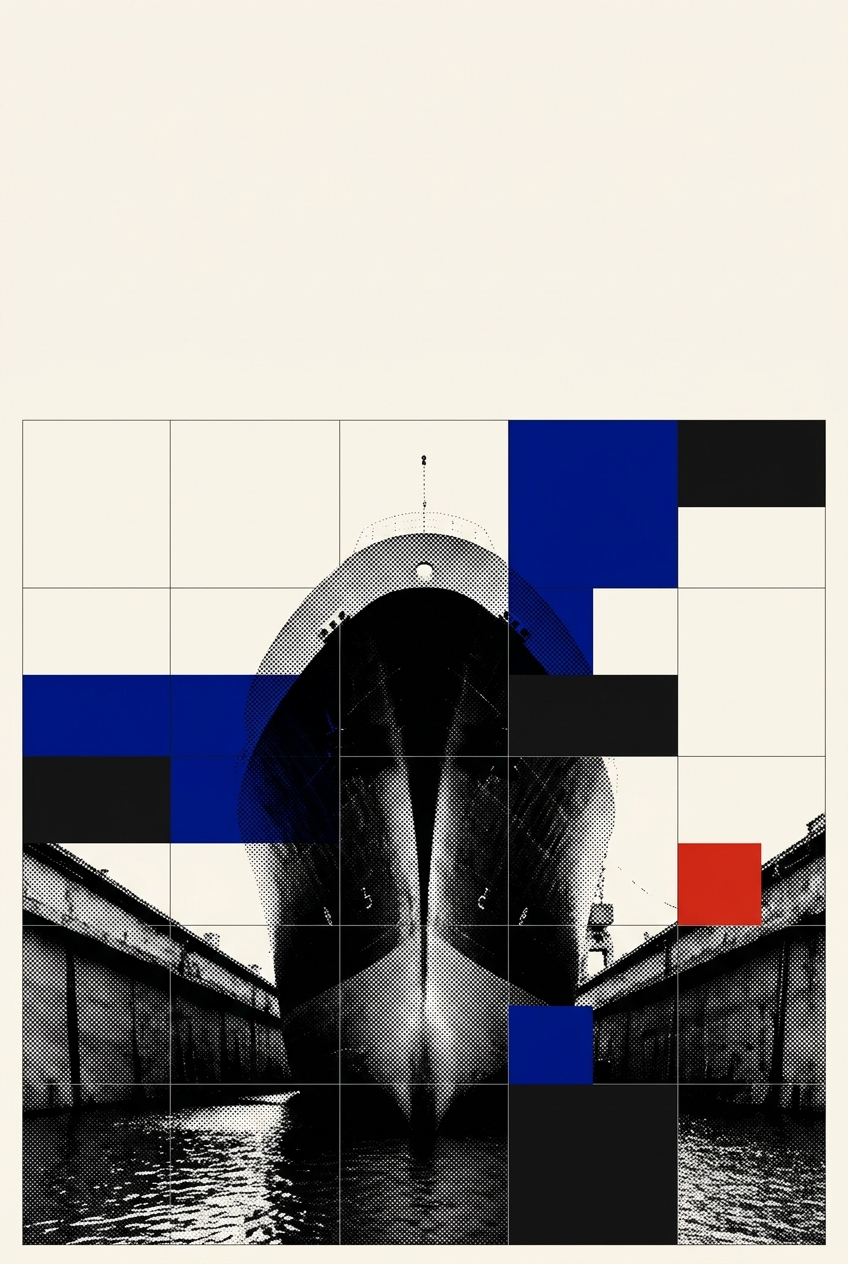
\includegraphics[width=\paperwidth,height=\paperheight]{plates/swiss/cover.jpg}}}}{%
    \PackageError{pd-swiss-plates}{Missing plate render plates/swiss/cover.jpg}{Generate the Swiss cover render and place it at plates/swiss/cover.jpg before building.}}}
\newcommand{\pdswisspartplate}[2]{% #1 numeral I..IV, #2 width
  \IfFileExists{plates/swiss/part-#1.jpg}{%
    \includegraphics[width=#2]{plates/swiss/part-#1.jpg}}{%
    \PackageError{pd-swiss-plates}{Missing plate render plates/swiss/part-#1.jpg}{Generate the Swiss part plate render and place it at plates/swiss/part-#1.jpg before building.}}}
\newcommand{\pdswissplate}[2]{% #1 chapter prefix, #2 width
  \IfFileExists{plates/swiss/chapter-#1.jpg}{%
    \includegraphics[width=#2]{plates/swiss/chapter-#1.jpg}%
  }{%
    \PackageError{pd-swiss-plates}{Missing plate render plates/swiss/chapter-#1.jpg}{Generate the Swiss chapter plate render and place it at plates/swiss/chapter-#1.jpg before building.}%
  }%
}
\newcommand{\pdswissfigplate}[2]{% #1 figure name, #2 width
  \IfFileExists{plates/swiss/#1.jpg}{%
    \includegraphics[width=#2]{plates/swiss/#1.jpg}%
  }{%
    \PackageError{pd-swiss-plates}{Missing figure plate render plates/swiss/#1.jpg}{Generate the Swiss figure plate render and place it at plates/swiss/#1.jpg before building.}%
  }%
}
\providecolor{pdswissred}{HTML}{DA291C}
\providecolor{pdcobalt}{HTML}{001489}
\providecolor{hhink}{HTML}{1B1712}
\providecolor{hhgray}{HTML}{5C5650}

% Canonical Landmark titles and pull-quotes
\expandafter\def\csname pdlandmarktitle@01\endcsname{Agentic Psychosis \& Hallucination Cascade}
\expandafter\def\csname pdlandmarkconcept@01\endcsname{Belief Drift \& Hallucination Cascades}
\expandafter\def\csname pdlandmarkquestion@01\endcsname{Can an unanchored swarm deliberate without spiraling into shared delusion?}
\expandafter\def\csname pdlandmarkquote@01\endcsname{When an unanchored swarm feeds on its own unverified assertions, error does not dissipate; it cascades into conviction. Coordination requires shared physical truth, not mutual agreement on hallucinated state.}

\expandafter\def\csname pdlandmarktitle@02\endcsname{Agentic Continuity \& The Overlapping Strand}
\expandafter\def\csname pdlandmarkconcept@02\endcsname{Substrate Continuity \& Overlapping Strands}
\expandafter\def\csname pdlandmarkquestion@02\endcsname{When every token and worker dies, what actually holds identity across time?}
\expandafter\def\csname pdlandmarkquote@02\endcsname{Identity is not an indivisible core preserved across time, but the continuous overlap of many short fibers. No single thread runs the full length of the rope; the strength is entirely in the friction between the splices.}

\expandafter\def\csname pdlandmarktitle@03\endcsname{The Engine Swap}
\expandafter\def\csname pdlandmarkconcept@03\endcsname{The Engine Swap \& Model Portability}
\expandafter\def\csname pdlandmarkquestion@03\endcsname{Can you replace the brain of a running system while keeping all its commitments intact?}
\expandafter\def\csname pdlandmarkquote@03\endcsname{The intelligence engine may be unbolted and swapped out in mid-voyage. What survives the swap is not the neural weights, but the unbroken hull of contracts, claims, and verified ledger obligations.}

\expandafter\def\csname pdlandmarktitle@04\endcsname{The Front-Loaded Probation Cliff}
\expandafter\def\csname pdlandmarkconcept@04\endcsname{The Front-Loaded Probation Cliff}
\expandafter\def\csname pdlandmarkquestion@04\endcsname{Why should an operating system ever trust an unverified autonomous actor?}
\expandafter\def\csname pdlandmarkquote@04\endcsname{Autonomy is never granted on faith; it is won against a sheer cliff of probation. The newcomer faces strict confinement until its attestation record proves it will not compromise the commons.}

\expandafter\def\csname pdlandmarktitle@05\endcsname{The Single-Writer Monotonic Horizon}
\expandafter\def\csname pdlandmarkconcept@05\endcsname{The Single-Writer Monotonic Horizon}
\expandafter\def\csname pdlandmarkquestion@05\endcsname{How do distributed agents agree on what happened first without Byzantine consensus?}
\expandafter\def\csname pdlandmarkquote@05\endcsname{One writer, one lock, one monotonic frontier. Beyond the commit horizon, the unwritten future remains empty paper; behind it, no write may ever be undone, denied, or reordered.}

\expandafter\def\csname pdlandmarktitle@06\endcsname{The Attenuation Frontier \& Cryptographic Macaroons}
\expandafter\def\csname pdlandmarkconcept@06\endcsname{The Attenuation Frontier \& Macaroons}
\expandafter\def\csname pdlandmarkquestion@06\endcsname{How do permissions travel across machines without accidentally widening?}
\expandafter\def\csname pdlandmarkquote@06\endcsname{Every delegation narrows the aperture of authority. A bearer credential cannot expand its reach as it traverses the network; it can only accumulate cryptographic caveats that bind its hands.}

\expandafter\def\csname pdlandmarktitle@07\endcsname{Attestation Without Revelation (The Sealed Harbor)}
\expandafter\def\csname pdlandmarkconcept@07\endcsname{Attestation Without Revelation (Sealed Harbor)}
\expandafter\def\csname pdlandmarkquestion@07\endcsname{Can a worker prove its computation was correct without revealing what it saw?}
\expandafter\def\csname pdlandmarkquote@07\endcsname{The enclave proves what was computed without disclosing what was seen. Trust in autonomous labor cannot demand total transparency; it demands unforgeable evidence of compliance.}

\expandafter\def\csname pdlandmarktitle@08\endcsname{Read-Poverty \& The Legible Swarm}
\expandafter\def\csname pdlandmarkconcept@08\endcsname{Read-Poverty \& Stigmergic Signaling}
\expandafter\def\csname pdlandmarkquestion@08\endcsname{Why is an agent that reads everything destined to bankrupt its operator?}
\expandafter\def\csname pdlandmarkquote@08\endcsname{In an ocean of synthetic prose, reading is infinitely more expensive than writing. A legible swarm does not shout across channels; it leaves quiet, structured pheromones in the environment.}

\expandafter\def\csname pdlandmarktitle@09\endcsname{Skills as Capital vs.\ Token Labor}
\expandafter\def\csname pdlandmarkconcept@09\endcsname{Skills as Capital vs. Perishable Token Labor}
\expandafter\def\csname pdlandmarkquestion@09\endcsname{When does prompt deliberation become too expensive compared to compiled code?}
\expandafter\def\csname pdlandmarkquote@09\endcsname{Token generation is perishable labor; compiled deterministic tools are durable capital. An economy matures when agents stop paying per token to deliberate and start amortizing proven apparatus.}

\expandafter\def\csname pdlandmarktitle@10\endcsname{The Bonded Commons \& Sacrificial Slashing}
\expandafter\def\csname pdlandmarkconcept@10\endcsname{The Bonded Commons \& Sacrificial Slashing}
\expandafter\def\csname pdlandmarkquestion@10\endcsname{What stops an agent from promising the world and walking away from disaster?}
\expandafter\def\csname pdlandmarkquote@10\endcsname{Trust without collateral is wishful thinking. An agent stakes its bond in the escrow of the commons; when an invariant is breached, the tripwire snaps and the stake is forfeited without appeal.}

\expandafter\def\csname pdlandmarktitle@11\endcsname{Sheaf Laplacian Invariance \& Cycle Consistency}
\expandafter\def\csname pdlandmarkconcept@11\endcsname{Sheaf Laplacians \& Cycle Holonomy}
\expandafter\def\csname pdlandmarkquestion@11\endcsname{Can a network of liars agree locally on every edge while still being caught globally?}
\expandafter\def\csname pdlandmarkquote@11\endcsname{Local consistency along every pairwise edge does not guarantee global truth. When an assertion traverses a closed cycle of harbors and returns altered, the non-zero holonomy reveals the fraud.}

\expandafter\def\csname pdlandmarktitle@12\endcsname{The Zombie Reclaim \& Salvage Graveyard}
\expandafter\def\csname pdlandmarkconcept@12\endcsname{Zombie Salvage \& Dead-Man Leases}
\expandafter\def\csname pdlandmarkquestion@12\endcsname{When an agent crashes in the dark, who buries the body and recovers the locks?}
\expandafter\def\csname pdlandmarkquote@12\endcsname{The graveyard of abandoned sessions is the foundation of harbor resilience. When a heartbeat goes cold, no ghost may linger; the lease expires, the locks are salvaged, and the port is reclaimed.}

% Single-digit alias fallbacks
\expandafter\def\csname pdlandmarktitle@1\endcsname{\csname pdlandmarktitle@01\endcsname}
\expandafter\def\csname pdlandmarkconcept@1\endcsname{\csname pdlandmarkconcept@01\endcsname}
\expandafter\def\csname pdlandmarkquestion@1\endcsname{\csname pdlandmarkquestion@01\endcsname}
\expandafter\def\csname pdlandmarkquote@1\endcsname{\csname pdlandmarkquote@01\endcsname}

\expandafter\def\csname pdlandmarktitle@2\endcsname{\csname pdlandmarktitle@02\endcsname}
\expandafter\def\csname pdlandmarkconcept@2\endcsname{\csname pdlandmarkconcept@02\endcsname}
\expandafter\def\csname pdlandmarkquestion@2\endcsname{\csname pdlandmarkquestion@02\endcsname}
\expandafter\def\csname pdlandmarkquote@2\endcsname{\csname pdlandmarkquote@02\endcsname}

\expandafter\def\csname pdlandmarktitle@3\endcsname{\csname pdlandmarktitle@03\endcsname}
\expandafter\def\csname pdlandmarkconcept@3\endcsname{\csname pdlandmarkconcept@03\endcsname}
\expandafter\def\csname pdlandmarkquestion@3\endcsname{\csname pdlandmarkquestion@03\endcsname}
\expandafter\def\csname pdlandmarkquote@3\endcsname{\csname pdlandmarkquote@03\endcsname}

\expandafter\def\csname pdlandmarktitle@4\endcsname{\csname pdlandmarktitle@04\endcsname}
\expandafter\def\csname pdlandmarkconcept@4\endcsname{\csname pdlandmarkconcept@04\endcsname}
\expandafter\def\csname pdlandmarkquestion@4\endcsname{\csname pdlandmarkquestion@04\endcsname}
\expandafter\def\csname pdlandmarkquote@4\endcsname{\csname pdlandmarkquote@04\endcsname}

\expandafter\def\csname pdlandmarktitle@5\endcsname{\csname pdlandmarktitle@05\endcsname}
\expandafter\def\csname pdlandmarkconcept@5\endcsname{\csname pdlandmarkconcept@05\endcsname}
\expandafter\def\csname pdlandmarkquestion@5\endcsname{\csname pdlandmarkquestion@05\endcsname}
\expandafter\def\csname pdlandmarkquote@5\endcsname{\csname pdlandmarkquote@05\endcsname}

\expandafter\def\csname pdlandmarktitle@6\endcsname{\csname pdlandmarktitle@06\endcsname}
\expandafter\def\csname pdlandmarkconcept@6\endcsname{\csname pdlandmarkconcept@06\endcsname}
\expandafter\def\csname pdlandmarkquestion@6\endcsname{\csname pdlandmarkquestion@06\endcsname}
\expandafter\def\csname pdlandmarkquote@6\endcsname{\csname pdlandmarkquote@06\endcsname}

\expandafter\def\csname pdlandmarktitle@7\endcsname{\csname pdlandmarktitle@07\endcsname}
\expandafter\def\csname pdlandmarkconcept@7\endcsname{\csname pdlandmarkconcept@07\endcsname}
\expandafter\def\csname pdlandmarkquestion@7\endcsname{\csname pdlandmarkquestion@07\endcsname}
\expandafter\def\csname pdlandmarkquote@7\endcsname{\csname pdlandmarkquote@07\endcsname}

\expandafter\def\csname pdlandmarktitle@8\endcsname{\csname pdlandmarktitle@08\endcsname}
\expandafter\def\csname pdlandmarkconcept@8\endcsname{\csname pdlandmarkconcept@08\endcsname}
\expandafter\def\csname pdlandmarkquestion@8\endcsname{\csname pdlandmarkquestion@08\endcsname}
\expandafter\def\csname pdlandmarkquote@8\endcsname{\csname pdlandmarkquote@08\endcsname}

\expandafter\def\csname pdlandmarktitle@9\endcsname{\csname pdlandmarktitle@09\endcsname}
\expandafter\def\csname pdlandmarkconcept@9\endcsname{\csname pdlandmarkconcept@09\endcsname}
\expandafter\def\csname pdlandmarkquestion@9\endcsname{\csname pdlandmarkquestion@09\endcsname}
\expandafter\def\csname pdlandmarkquote@9\endcsname{\csname pdlandmarkquote@09\endcsname}

\newcommand{\pdswisslandmarkplate}[2]{% #1 landmark ID (e.g. 01..12), #2 width
  \IfFileExists{plates/swiss/landmark-#1.jpg}{%
    \centering
    \includegraphics[width=#2]{plates/swiss/landmark-#1.jpg}%
    \par\vspace{10pt}%
    \begin{minipage}{\linewidth}%
      {\color{pdcobalt}\rule{\linewidth}{1.2pt}}\par\vspace{6pt}%
      \raggedright
      {\color{pdswissred}\rule{4.5pt}{4.5pt}}\enspace%
      {\pdgrotesk\bfseries\scshape\fontsize{9}{11}\selectfont\color{hhink}%
        Landmark #1\enspace\textperiodcentered\enspace\csname pdlandmarktitle@#1\endcsname}\par\vspace{4.5pt}%
      {\pdgrotesk\itshape\fontsize{9.5}{13.5}\selectfont\color{hhink}%
        ``\csname pdlandmarkquote@#1\endcsname''\par}%
      \vspace{6pt}%
      {\color{hhgray!30}\rule{\linewidth}{0.4pt}}%
    \end{minipage}%
  }{%
    \PackageError{pd-swiss-plates}{Missing plate render plates/swiss/landmark-#1.jpg}{Generate the Swiss landmark plate render and place it at plates/swiss/landmark-#1.jpg before building.}}}
\makeatother

\fi
% Wordless interstitial art for the Swiss Book, not numbered evidence figures.
% Insert only at an authored paragraph boundary. On verso the plate faces
% following text; on recto it faces preceding text. Never split an arbitrary
% text page, paragraph, worked example, or proof to manufacture verso parity.
\makeatletter
\providecommand{\pdreflectionrecord}[2]{}
\providecommand*{\toclevel@pdplate}{1}
\definecolor{pdreflectionpanel}{HTML}{00564C}
% Interstitials have their own contents entry; they must not advance the
% chapter-art counter used by the illustrated chapter contents.
\newcommand{\pdreflectiontitle}[2]{%
  \expandafter\def\csname pd@reflection@title@#1\endcsname{#2}}
\pdreflectiontitle{the-unseen-boat}{What a summary leaves unseen}
\pdreflectiontitle{the-waiting-body}{What survives the worker}
\pdreflectiontitle{the-paper-crossing}{A commitment between independent shores}
\pdreflectiontitle{the-controlled-opening}{The controlled opening}
% Text-bearing plates declare their own reserved, opaque lower panel.
% Existing wordless plates do not acquire generic captions or title bars.
\newcommand{\pdreflectionbody}[2]{%
  \expandafter\def\csname pd@reflection@body@#1\endcsname{#2}}
\pdreflectionbody{the-controlled-opening}{%
  A closed cabinet still has a slot. A confined agent still has an output.
  The noninterference claim must name what that output may reveal and which
  other channels the model excludes.}
\newcommand{\pdreflectiontocentry}[2]{%
  \begin{minipage}[c]{.19\linewidth}%
    \includegraphics[width=\linewidth,height=.62in,keepaspectratio]{plates/interstitial/#1.png}%
  \end{minipage}\hfill
  \begin{minipage}[c]{.76\linewidth}\raggedright\small
    Plate: #2%
  \end{minipage}}
\newcommand*{\l@pdplate}[2]{%
  \par\addvspace{7pt}\noindent
  \begin{minipage}[c]{.90\linewidth}#1\end{minipage}\hfill
  \makebox[.07\linewidth][r]{\small #2}\par\addvspace{7pt}}
\newcommand{\pd@reflection@render}[1]{%
  \IfFileExists{plates/interstitial/#1.png}{%
    \thispagestyle{empty}%
    \ifcsname pd@reflection@title@#1\endcsname
      \phantomsection\label{plate:#1}%
    \else
      \PackageError{pd-reflection-plates}{Missing contents title for #1}%
        {Register this plate with pdreflectiontitle before placing it.}%
    \fi
    \protected@write\@auxout{}{\string\pdreflectionrecord{#1}{\thepage}}%
    \AddToShipoutPictureBG*{\AtPageCenter{\makebox(0,0){%
      \includegraphics[width=6in,height=9in,keepaspectratio]{plates/interstitial/#1.png}}}}%
    \ifcsname pd@reflection@body@#1\endcsname
      \AddToShipoutPictureFG*{\AtPageCenter{\makebox(0,0){\begingroup
        % Page art is not a column figure. Undo the Book's centering wrapper,
        % as the existing full-page cover renderer does.
        \ifdefined\pd@typesetpicturebox\let\pgfsys@typesetpicturebox\pd@typesetpicturebox\fi
        \begin{tikzpicture}[x=1in,y=1in]
          \useasboundingbox (0,0) rectangle (6,9);
          \fill[pdreflectionpanel] (0,0) rectangle (6,2.45);
          \node[anchor=north west,inner sep=0,text=white,text width=5in,
            font=\fontsize{17}{21}\selectfont\bfseries] at (.5,2.05)
            {\csname pd@reflection@title@#1\endcsname};
          \node[anchor=north west,inner sep=0,text=white,text width=5in,
            font=\fontsize{11}{15}\selectfont,align=left] at (.5,1.5)
            {\raggedright\hyphenpenalty=10000\csname pd@reflection@body@#1\endcsname};
        \end{tikzpicture}\endgroup}}}%
    \fi
    \null\newpage
  }{\PackageError{pd-reflection-plates}{Missing interstitial plate #1}%
    {Restore plates/interstitial/#1.png and its provenance before building.}}%
}
\newcommand{\pd@reflection@place}[1]{%
  \clearpage
  \pd@reflection@render{#1}%
}
\newcommand{\pdreflectionplate}[1]{%
  \ifpdswiss\pd@reflection@place{#1}\fi
}
\makeatother


% The maturity, guarantee, proof-obligation and claim-evidence vocabularies --
% \Built, \BuiltWeak, \Designed, \Vision, their uppercase aliases, \NotGuar,
% \Closed, \Partial, \Open, \SpecOnly, \Verified, \Proved, \Unproved -- and
% \code are defined once, for this volume and for every standalone chapter, in
% figures/pd-pedagogy.tex (\input above).
%
% They used to be listed here AND again in each chapter's own preamble. The
% generator keeps only what lies between \begin{document} and \end{document},
% so the chapter copies never reached this document and the two sets were free
% to disagree -- which they did: chapter 4 printed "built" and "designed" when
% it compiled alone and "implemented" and "specified" at the same call sites
% here. One definition, in a file both preambles read, is what makes a marker
% mean the same thing in both places.
% scripts/harbor-research/check_duplicate_macros.py fails the build if a
% second definition of any of these names comes back.

\newcommand{\pullquote}[1]{%
  \par\vspace{6pt}\noindent\begin{tikzpicture}
  \node[draw=none,fill=hhsand!22,inner sep=10pt,text width=\dimexpr\textwidth-30pt\relax,align=left] (q) {\itshape\large #1};
  \draw[hhcobalt,line width=2.5pt] (q.north west) -- (q.south west);
  \end{tikzpicture}\par\vspace{6pt}}
\newcommand{\keyidea}[1]{%
  \par\vspace{6pt}\noindent\begin{tikzpicture}
  \node[draw=none,fill=hhsand!18,rounded corners=2pt,inner sep=9pt,text width=\dimexpr\textwidth-26pt\relax,align=left] (k)
        {{\scshape\bfseries\color{hhgray}\small Key idea.}\enspace #1};
  \draw[hhgray!60,line width=1pt] (k.north west) -- (k.south west);
  \end{tikzpicture}\par\vspace{6pt}}
\newcommand{\pitfall}[1]{%
  \par\vspace{6pt}\noindent\begin{tikzpicture}
  \node[draw=none,fill=hhsand!18,rounded corners=2pt,inner sep=9pt,text width=\dimexpr\textwidth-26pt\relax,align=left] (p)
        {{\scshape\bfseries\color{hhcobalt}\small Pitfall.}\enspace #1};
  \draw[hhgray!60,line width=1pt] (p.north west) -- (p.south west);
  \end{tikzpicture}\par\vspace{6pt}}
\newcommand{\xrefbox}[1]{%
  \vspace{4pt}\noindent\begin{tikzpicture}
  \node[draw=hhgray!45,line width=0.4pt,fill=hhsand!18,rounded corners=2pt,inner sep=8pt,text width=\dimexpr\textwidth-22pt\relax,align=left]{\small #1};
  \end{tikzpicture}\vspace{4pt}}
\newcommand{\scene}[2]{%
  \par\vspace{8pt plus 2pt}\noindent\begin{tcolorbox}[
    enhanced, breakable, sharp corners,
    colback=white, colframe=black,
    boxrule=0.5pt, leftrule=3.2pt,
    left=9pt, right=9pt, top=7pt, bottom=7pt,
    before skip=6pt, after skip=6pt
  ]%
  \noindent{\small\raisebox{-2pt}{\IfFileExists{figures/icons/mira-silhouette.pdf}{
\includegraphics[height=1.35em]{figures/icons/mira-silhouette.pdf}}{\IfFileExists{figures/icons/mira-silhouette.png}{
\includegraphics[height=1.35em]{figures/icons/mira-silhouette.png}}{}}}\enspace{\scshape\bfseries\color{black}Scene}\enspace\textperiodcentered\enspace{\bfseries #1}\pdblockheadingend{\itshape #2}}%
  \end{tcolorbox}\par\vspace{8pt plus 2pt}}
\newcommand{\openstar}{{\textcolor{hhcobalt}{$\bigstar$}}\;}
\newcommand{\exhead}[1]{\par\vspace{4pt}\noindent{\scshape\bfseries\color{hhink}#1}\par\vspace{-2pt}}

% Chapter-local exercise idioms keep authored semantics under one visual grammar.
\newenvironment{lsexercises}{%
  \par\vspace{8pt}\noindent\begin{tikzpicture}
  \node[draw=hhgray!45,line width=0.4pt,fill=hhsand!12,rounded corners=2pt,inner sep=10pt,text width=\dimexpr\textwidth-28pt\relax,align=left]\bgroup
  \begin{minipage}{\dimexpr\textwidth-30pt\relax}
  {\scshape\bfseries\color{hhink}Exercises}\par\vspace{3pt}\small
}{\end{minipage}\egroup;\end{tikzpicture}\par\vspace{8pt}}
\newenvironment{stpexercises}{%
  \par\vspace{8pt}\noindent\begin{tikzpicture}
  \node[draw=hhgray!45,line width=0.4pt,fill=hhsand!12,rounded corners=2pt,inner sep=10pt,text width=\dimexpr\textwidth-26pt\relax,align=left]\bgroup
  \begin{minipage}{\dimexpr\textwidth-46pt\relax}
  {\scshape\bfseries\color{hhink}\large Exercises}\par\vspace{3pt}\small
}{\end{minipage}\egroup;\end{tikzpicture}\par\vspace{8pt}}
\newenvironment{heexercises}{%
  \par\vspace{8pt}\noindent
  {\scshape\bfseries\textcolor{hhink}{\textcolor{hhgray!70}{\rule[-1pt]{2.5pt}{11pt}}\enspace Exercises}}
  \par\nobreak\vspace{2pt}
  \begin{enumerate}[label=\textbf{E\arabic*.},leftmargin=2.6em,itemsep=2pt,topsep=2pt]
}{\end{enumerate}\vspace{6pt}}
\newcommand{\swkexercises}[1]{%
  \par\vspace{8pt}\noindent\begin{tikzpicture}
  \node[draw=hhgray!45,line width=0.4pt,fill=hhsand!12,rounded corners=2pt,inner sep=9pt,text width=\dimexpr\textwidth-26pt\relax,align=left]
        {{\scshape\bfseries\textcolor{hhink}{Exercises.}}\par\vspace{3pt}#1};
  \end{tikzpicture}\par\vspace{6pt}}

% Code and pseudocode as a printed book sets them: an indented block in a
% dense monospace with tight leading, keywords bold, comments italic grey,
% small grey line numbers, no frame, no background, no stripes. A wrapped
% line continues under a small grey hook.
\lstdefinestyle{pdcode}{language=C,backgroundcolor={},frame=none,
  basicstyle=\ttfamily\fontsize{8.6}{10.6}\selectfont,columns=fullflexible,keepspaces=true,
  keywordstyle=\bfseries,commentstyle=\color{hhgray}\itshape,
  stringstyle=\color{hhink!70!hhgray},numbers=left,numberstyle=\fontsize{6.5}{7}\selectfont\color{hhgray},
  numbersep=7pt,breaklines=true,breakatwhitespace=false,breakindent=1.6em,
  postbreak=\mbox{\textcolor{hhgray}{\fontsize{7}{7}\selectfont$\hookrightarrow$}\space},
  showstringspaces=false,tabsize=2,aboveskip=7pt,belowskip=5pt,
  xleftmargin=1.9em,xrightmargin=0pt,captionpos=b}
\lstdefinestyle{pseudocode}{style=pdcode,
  morekeywords={function,return,if,then,else,for,while,do,begin,end,atomic,transaction,reject,commit,assert,raise}}
\lstdefinestyle{proverif}{style=pdcode}
\lstdefinestyle{rust}{style=pdcode,tabsize=4}
\lstdefinestyle{tlaplus}{style=pdcode,
  morekeywords={MODULE,EXTENDS,CONSTANTS,VARIABLES,VARIABLE,Init,Next,Spec,
  TypeOK,IF,THEN,ELSE,LET,IN,CHOOSE,SUBSET,UNION,DOMAIN,EXCEPT,
  UNCHANGED,TRUE,FALSE,BOOLEAN,Nat,Int,STRING,Seq,Append,Len,Head,Tail,
  ENABLED,WF_,SF_,THEOREM,ASSUME,INSTANCE,WITH,LOCAL}}
\lstset{style=pdcode}

% Shared presentation primitives, loaded without adopting the broader semantic
% or margin-layout changes. Only protocols opt into the frame and glyph here.
% Presentation only. Official Lucide assets: figures/lucide/LICENSE.
\makeatletter
\definecolor{pdblockProof}{HTML}{B33F35}
\definecolor{pdblockProperty}{HTML}{7048A5}
\definecolor{pdblockHypothesis}{HTML}{427A26}
\definecolor{pdblockCalculation}{HTML}{946000}
\definecolor{pdblockInvariant}{HTML}{233A76}
\definecolor{pdblockDefinition}{HTML}{3D454B}
\definecolor{pdblockChecked}{HTML}{006EA0}
\definecolor{pdblockProtocol}{HTML}{007D73}
\definecolor{pdblockNeutral}{HTML}{363B40}
\ifdefined\pdblockfamily\else
\newcommand{\pdblockfamily}[1]{%
  \def\pdblock@family{#1}%
  \ifdefstring{\pdblock@family}{Conjecture}{\def\pdblock@family{Empirical hypothesis}}{}%
  \def\pdblock@color{pdblockNeutral}\def\pdblock@icon{file-text}%
  \ifdefstring{\pdblock@family}{Theorem}{\def\pdblock@color{pdblockProof}\def\pdblock@icon{scroll-text}}{}%
  \ifdefstring{\pdblock@family}{Lemma}{\def\pdblock@color{pdblockProof}\def\pdblock@icon{scroll-text}}{}%
  \ifdefstring{\pdblock@family}{Proposition}{\def\pdblock@color{pdblockProof}\def\pdblock@icon{scroll-text}}{}%
  \ifdefstring{\pdblock@family}{Corollary}{\def\pdblock@color{pdblockProof}\def\pdblock@icon{scroll-text}}{}%
  \ifdefstring{\pdblock@family}{Property}{\def\pdblock@color{pdblockProperty}\def\pdblock@icon{key-round}}{}%
  \ifdefstring{\pdblock@family}{Definition}{\def\pdblock@color{pdblockDefinition}\def\pdblock@icon{book-open}}{}%
  \ifdefstring{\pdblock@family}{Empirical hypothesis}{\def\pdblock@color{pdblockHypothesis}\def\pdblock@icon{flask-conical}}{}%
  \ifdefstring{\pdblock@family}{Numbers by hand}{\def\pdblock@color{pdblockCalculation}\def\pdblock@icon{calculator}}{}%
  \ifdefstring{\pdblock@family}{Design invariant}{\def\pdblock@color{pdblockInvariant}\def\pdblock@icon{lock-keyhole}}{}%
  \ifdefstring{\pdblock@family}{Model-checked property}{\def\pdblock@color{pdblockChecked}\def\pdblock@icon{list-checks}}{}%
  \ifdefstring{\pdblock@family}{Protocol}{\def\pdblock@color{pdblockProtocol}\def\pdblock@icon{workflow}}{}%
}
\fi
\providecommand{\pdblock@inlinebegin}{%
  \ifcsname pd@typesetpicturebox\endcsname
    \let\pgfsys@typesetpicturebox\pd@typesetpicturebox
  \fi}
\providecommand{\pdblockglyph}[1]{\begingroup
  \edef\pdblock@expanded{#1}\expandafter\pdblockfamily\expandafter{\pdblock@expanded}%
  \raisebox{-2.2pt}{\includegraphics[width=12pt,height=12pt]{figures/lucide/\pdblock@icon.pdf}}%
  \endgroup\hspace{.45em}}
% Every split segment keeps a full-strength 0.5pt perimeter for the Book inks.
% The retained 2% field and corner geometry are specific to this protocol slice.
% The colored upper-left cap
% is longer than its upright; the lower-right upright is longer than its cap.
\providecommand{\pdblock@frame}{%
  \draw[draw=\pdblock@color,line width=.5pt]
    (frame.south west) rectangle (frame.north east);
  \fill[\pdblock@color] (frame.north west) rectangle
    ([xshift=32pt,yshift=-3pt]frame.north west);
  \fill[\pdblock@color] (frame.north west) rectangle
    ([xshift=3pt,yshift=-16pt]frame.north west);
  \fill[\pdblock@color] (frame.south east) rectangle
    ([xshift=-16pt,yshift=3pt]frame.south east);
  \fill[\pdblock@color] (frame.south east) rectangle
    ([xshift=-3pt,yshift=28pt]frame.south east);}
\providecommand{\pdblockbefore}[1]{%
  \par\if@nobreak\else\Needspace{5\baselineskip}\fi
  \begingroup
  \edef\pdblock@expanded{#1}\expandafter\pdblockfamily\expandafter{\pdblock@expanded}%
  \pdblock@inlinebegin
  \begin{tcolorbox}[enhanced,breakable,sharp corners,frame hidden,
    colback=\pdblock@color!2!white,boxrule=.45pt,boxsep=0pt,
    left=8pt,right=8pt,top=7pt,bottom=7pt,
    before skip=8pt plus 2pt,after skip=8pt plus 2pt,
    pad at break*=7pt,lines before break=6,
    overlay unbroken={\pdblock@frame},overlay first={\pdblock@frame},
    overlay middle={\pdblock@frame},overlay last={\pdblock@frame}]
    \clubpenalty=9000 \widowpenalty=9000
    \displaywidowpenalty=9000 \brokenpenalty=9000
}
\providecommand{\pdblockafter}[1]{\par\end{tcolorbox}\endgroup}
\makeatother


% Fixed, restrained theorem skips keep theorem/prose transitions on the same
% baseline cadence. A block heading is separate from its first body paragraph.
% amsthm's class defaults carry highly stretchable vertical
% glue, which produced visibly unrelated gaps at page breaks in chapter 7.
\newtheoremstyle{pddefinition}% name
  {7pt plus 1pt minus 1pt}{7pt plus 1pt minus 1pt}% above / below
  {\normalfont}{}% body / indent
  {\bfseries}{.}{0pt}{\pdblockglyph{#1}\thmname{#1}\thmnumber{\ #2}\thmnote{\hspace{.35em}(#3)}}% head
\newtheoremstyle{pdplain}% name
  {7pt plus 1pt minus 1pt}{7pt plus 1pt minus 1pt}% above / below
  {\itshape}{}% body / indent
  {\bfseries}{.}{0pt}{\pdblockglyph{#1}\thmname{#1}\thmnumber{\ #2}\thmnote{\hspace{.35em}(#3)}}% head
\newtheoremstyle{pdremark}% name
  {6pt plus 1pt minus 1pt}{6pt plus 1pt minus 1pt}% above / below
  {\normalfont}{}% body / indent
  {\itshape}{.}{0pt}{\pdblockglyph{#1}\thmname{#1}\thmnumber{\ #2}\thmnote{\hspace{.35em}(#3)}}% head

\newtheoremstyle{pdprotocol}
  {7pt plus 1pt minus 1pt}{7pt plus 1pt minus 1pt}
  {\normalfont}{}{\bfseries}{.}{0pt}
  {\pdblockglyph{Protocol}\thmname{#1}\thmnumber{\ #2}\thmnote{\hspace{.35em}(#3)}}
\makeatletter
\newcommand{\pdprotocolheadingend}{%
  \par\nobreak\smallskip\@afterindentfalse\@afterheading\ignorespaces}
% AtBeginEnvironment runs inside the environment group, before amsthm builds
% its deferred heading. Flush that heading, then end its paragraph even when
% the body begins with a list. Preserve nameref's wrapper and restore the entry
% and heading renderer immediately, so nested unrelated families are unchanged.
\newcommand{\pdprotocolparagraphs}{%
  \let\pdprotocolsavedentry\@begintheorem
  \let\pdprotocolsavedhead\thmhead
  \apptocmd{\@begintheorem}{\leavevmode\pdprotocolheadingend
    \let\@begintheorem\pdprotocolsavedentry
    \let\thmhead\pdprotocolsavedhead\ignorespaces}{}%
    {\PackageError{pdprotocol}{Cannot terminate the protocol heading}{Check the amsthm entry point.}}}
\AtBeginEnvironment{protocol}{\pdprotocolparagraphs}
\AtBeginEnvironment{heprotocol}{\pdprotocolparagraphs}
\makeatother

\theoremstyle{definition}
\newtheorem{definition}{Definition}[section]
\newtheorem{property}{Property}[section]
\theoremstyle{pdprotocol}
\newtheorem{protocol}{Protocol}[section]
\theoremstyle{plain}
\newtheorem{theorem}{Theorem}[section]
\newtheorem{lemma}{Lemma}[section]
\newtheorem{proposition}{Proposition}[section]
\newtheorem{corollary}{Corollary}[section]
\newtheorem{conjecture}{Conjecture}[section]
\theoremstyle{remark}
\newtheorem*{remark}{Remark}
% Flush amsthm's deferred label into its own paragraph before body tokens.
% A head-separator newline alone leaves an opening list's marker on the head.
\makeatletter
\patchcmd{\@begintheorem}{\ignorespaces}{\leavevmode\pdblockheadingend}{}%
  {\PackageError{pd-book}{Theorem heading paragraph patch failed}{Check the amsthm heading definition.}}
\makeatother
% Keep the usual proof/QED machinery, but separate the proof heading too.
\expandafter\patchcmd\csname\string\proof\endcsname
  {\ignorespaces}{\leavevmode\pdblockheadingend}{}%
  {\PackageError{pd-book}{Proof heading paragraph patch failed}{Check the amsthm proof definition.}}
\BeforeBeginEnvironment{protocol}{\pdblockbefore{Protocol}}
\AfterEndEnvironment{protocol}{\pdblockafter{Protocol}}


\newcounter{lsprotocol}[section]
\renewcommand{\thelsprotocol}{\thesection.\arabic{lsprotocol}}
% Protocol prose is not a drawing: a TikZ/minipage wrapper made the whole
% passage indivisible and left half-pages empty. Both chapter variants now
% share one breakable frame while keeping their counters and labels intact.
\newenvironment{pdbookprotocol}[2]{%
  \pdblockbefore{Protocol}%
  % The destination belongs inside the frame, after its start reservation.
  \refstepcounter{#1}%
  \noindent{\raggedright\normalfont\bfseries\color{hhink}\pdblockglyph{Protocol}%
    Protocol~\csname the#1\endcsname\ifblank{#2}{}{\hspace{.35em}(#2)}.\par}%
  \small\pdprotocolheadingend
}{\pdblockafter{Protocol}}
\newenvironment{lsprotocol}[1]{%
  \begin{pdbookprotocol}{lsprotocol}{#1}%
}{\end{pdbookprotocol}}
\newcounter{stpprotocol}[section]
\renewcommand{\thestpprotocol}{\thesection.\arabic{stpprotocol}}
\newenvironment{stpprotocol}[1][]{%
  \begin{pdbookprotocol}{stpprotocol}{#1}%
}{\end{pdbookprotocol}}
\theoremstyle{pdprotocol}
\newtheorem{heprotocol}{Protocol}[section]
\BeforeBeginEnvironment{heprotocol}{\pdblockbefore{Protocol}}
\AfterEndEnvironment{heprotocol}{\pdblockafter{Protocol}}
\theoremstyle{definition}

\tikzset{
  stp box/.style={draw=hhink,line width=0.55pt,fill=hhsand!22,rounded corners=2pt,inner sep=7pt,align=center,minimum height=10mm},
  stp accent box/.style={stp box,draw=hhcobalt,line width=0.9pt},
  stp arrow/.style={-{Stealth[length=2.3mm,width=1.5mm]},draw=hhink,line width=0.65pt},
  stp accent arrow/.style={-{Stealth[length=2.3mm,width=1.5mm]},draw=hhcobalt,line width=0.8pt},
  stp dashed arrow/.style={stp accent arrow,dashed},
  stp label/.style={fill=hhpaper,inner xsep=3pt,inner ysep=1.5pt,font=\footnotesize\itshape,text=hhgray},
  stp heading/.style={font=\footnotesize\bfseries,text=hhink},
  stp status/.style={font=\scriptsize\scshape,text=hhgray},
}

\pagestyle{fancy}
\fancyhf{}
\fancyhead[RE,LO]{\small\itshape\color{hhgray} \pdshorttitle}
\fancyhead[LE,RO]{\small\color{hhgray}\thepage}
\fancyfoot[C]{\footnotesize\color{hhgray} Textbook Edition \textperiodcentered\ \pdeditiondate}
\renewcommand{\headrulewidth}{0.4pt}
\renewcommand{\footrulewidth}{0pt}
% Backmatter replaces all chapter heads on both sides of the spread.
\newcommand{\pdbackmatterheaders}[1]{%
  \fancyhead{}%
  \fancyhead[LE,RO]{\small\color{hhgray}\thepage}%
  \fancyhead[RE,LO]{\small\itshape\color{hhgray} #1}%
  \fancyfoot[C]{\footnotesize\color{hhgray}\pdeditiontitle\ \textperiodcentered\ #1}}

% ---- Chapters, parts, and the front-matter map ----------------------------
% Chapter numbers are Arabic and come from whitepaper/textbook.json via the
% generator: \pdchapter{number}{title}{prefix}{hue}. The prefix selects the
% chapter's seam rails and its entry in figures/pd-textbook-map.tex (question,
% epigraph, one-breath answer, part label); the hue is the PART's, inherited by
% every chapter in it, so each part owns one color and nothing dilutes it.
\newcounter{pdchapter}
\renewcommand{\thepdchapter}{\arabic{pdchapter}}
\makeatletter
\@namedef{theHpdchapter}{chap.\arabic{pdchapter}}
\makeatother
\newcommand{\pdcurrentchapter}{0}
\newcommand{\pdcurrentchaptercolor}{pdcobalt}
% A live link to a chapter, by prefix. figures/pd-hyperlinks.tex provides the
% plain-text fallback for standalone chapters; the Book defines the real thing.
\DeclareRobustCommand{\pdchaplink}[2]{\hyperref[chap:#1]{#2}}

% Begin the next material on a verso so a two-page construction is a physical
% facing spread. \cleardoublepage does the opposite: it begins on a recto.
\newcommand{\cleartoleftpage}{%
  \clearpage
  \ifodd\value{page}\thispagestyle{empty}\null\newpage\fi}

% The weighted four-hue rule. One segment per part, its length proportional to
% the part's share of the book's pages (from the page references once they
% exist; chapter counts on the first pass). Segments up to the current part are
% solid, the rest outlined, so the same rule reads as a progress mark on part
% and chapter openers and as the whole book on the title page.
%   \pdweightrule[color]{current part index or 0 for all}{total width}{height}
\newdimen\pdweightx
\newdimen\pdweightw
\newcount\pdweighti
\makeatletter
\newcommand{\pdweightrule}[4][]{%
  \begingroup
  \edef\pd@tot{\the\numexpr\getpagerefnumber{book:appendices}-\getpagerefnumber{part:\pdfirstpartnumeral}\relax}%
  \ifnum\pd@tot<1 \def\pd@tot{0}\fi
  \pdweightx=0pt \pdweighti=0
  \def\pdweightsegment##1##2##3##4{%
    \advance\pdweighti by 1
    \ifnum\pd@tot>0
      \edef\pd@seg{\the\numexpr\getpagerefnumber{##3}-\getpagerefnumber{part:##1}\relax}%
      \ifnum\pd@seg<1 \edef\pd@seg{##4}\edef\pd@den{\pdchaptercount}\else\edef\pd@den{\pd@tot}\fi
    \else
      \edef\pd@seg{##4}\edef\pd@den{\pdchaptercount}%
    \fi
    \pdweightw=\dimexpr(#3-3pt*(\pdpartcount-1))*\pd@seg/\pd@den\relax
    \if\relax\detokenize{#1}\relax\def\pd@col{##2}\else\def\pd@col{#1}\fi
    \ifnum#2=0 \def\pd@solid{1}\else\ifnum\pdweighti>#2 \def\pd@solid{0}\else\def\pd@solid{1}\fi\fi
    \if1\pd@solid
      \fill[color=\pd@col] (\the\pdweightx,0pt) rectangle ++(\the\pdweightw,#4);
    \else
      \draw[color=\pd@col,line width=0.5pt] (\the\dimexpr\pdweightx+0.25pt\relax,0.25pt) rectangle ++(\the\dimexpr\pdweightw-0.5pt\relax,\the\dimexpr#4-0.5pt\relax);
    \fi
    \advance\pdweightx by \pdweightw \advance\pdweightx by 3pt
  }%
  \begin{tikzpicture}[baseline=0pt]
    \pdweightsegmentslist
  \end{tikzpicture}%
  \endgroup}
\makeatother

% The chapter opener: one page with the title, an epigraph, a plate when the
% chapter has one, and the question the chapter answers with its one-breath
% answer. Nothing else. The chapter's first section starts on the next page.
\makeatletter
\def\pd@chapter@maritime#1#2#3#4{%
  \vspace*{0.1cm}
  \noindent{\scshape\footnotesize\color{hhgray}\ifnum#1=0 Chapter 0\hfill\pdchapterpartlabel\else Chapter #1 of \pdchaptercount\hfill\pdchapterpartlabel\fi}\par
  \vspace{0.25cm}
  \noindent\pdweightrule{\pdchapterpartindex}{\textwidth}{2pt}\par
  % The gilt fillet: the trim line of the engraved plates, carried onto the
  % page. Hairline, under the weight rule, and nowhere else on the spread.
  \vspace{2.6pt}\noindent{\color{pdmaritimegold}\rule{\textwidth}{0.4pt}}\par
  \vspace{\dimexpr1.3cm-3pt\relax}
  {\noindent\fontsize{34}{40}\selectfont\color{hhink}\hyphenpenalty=10000\exhyphenpenalty=10000\raggedright #2\par}
  \vspace{1.0cm}
  \begin{flushright}
    \begin{minipage}{0.84\textwidth}\raggedleft
      {\itshape\pdchapterepigraph\par}
      \vspace{5pt}
      {\footnotesize\scshape\color{hhgray}\pdchapterepigraphsource\par}
    \end{minipage}
  \end{flushright}
  % The question block is measured first, then the plate takes what the page
  % still has above it (capped at 0.42 of the text height), and the question
  % closes the page as in the first printing. Nothing can spill: the plate is
  % cut to fit and dropped below 3 cm.
  \sbox{\pdqbox}{\begin{minipage}{\textwidth}
    \noindent{\scshape\footnotesize\color{hhgray}The question this chapter answers}\par
    \vspace{6pt}
    {\noindent\fontsize{21}{26}\selectfont\color{hhink}\hyphenpenalty=10000\exhyphenpenalty=10000\raggedright\pdchapterquestion\par}
    \vspace{9pt}
    {\noindent\small\itshape\pdchapteroneline\par}
  \end{minipage}}%
  \par
  \IfFileExists{plates/chapter-#3.jpg}{%
    \ifdim\pagegoal=\maxdimen
      \setlength{\pdplateh}{\dimexpr\textheight-\pagetotal\relax}%
    \else
      \setlength{\pdplateh}{\dimexpr\pagegoal-\pagetotal\relax}%
    \fi
    \addtolength{\pdplateh}{-\ht\pdqbox}\addtolength{\pdplateh}{-\dp\pdqbox}\addtolength{\pdplateh}{-1.6cm}%
    \ifdim\pdplateh>0.42\textheight \setlength{\pdplateh}{0.42\textheight}\fi
    \ifdim\pdplateh>3cm
      \vspace{0.5cm}%
      \noindent\makebox[\textwidth]{\includegraphics[width=\textwidth,height=\pdplateh,keepaspectratio]{plates/chapter-#3.jpg}}\par
    \fi}{}%
  \vfill
  \noindent\usebox{\pdqbox}\par
  \vspace{0.2cm}
}
% swiss: a colour band carries number and title; the question sits on paper
\def\pd@chapter@swiss#1#2#3#4{%
  \begin{adjustwidth*}{0pt}{-\dimexpr\marginparsep+\marginparwidth\relax}
  \vspace*{-0.5cm}
  \noindent\begin{tikzpicture}
    \node[fill=#4,inner sep=0pt,minimum width=\linewidth,minimum height=0.36\textheight,anchor=north west] (band) at (0,0) {};
    \node[anchor=north west,text=hhpaper,font=\pdgrotesk\fontsize{9.5}{12}\selectfont\bfseries,inner sep=0pt]
      at (0.45cm,-0.5cm) {\ifnum#1=0 Chapter 0\quad\textperiodcentered\quad\pdchapterpartlabel\else Chapter #1 of \pdchaptercount\quad\textperiodcentered\quad\pdchapterpartlabel\fi};
    \node[anchor=south west,text=hhpaper,font=\pddisplayface\fontsize{78}{78}\selectfont\bfseries,inner sep=0pt]
      at (0.4cm,{-0.36\textheight+3.0cm}) {#1};
    \node[anchor=south west,text=hhpaper,font=\pddisplayface\fontsize{27}{31}\selectfont\bfseries,inner sep=0pt,
      text width={\dimexpr\linewidth-1cm\relax},align=left] at (0.45cm,{-0.36\textheight+0.55cm}) {#2};
  \end{tikzpicture}\par
  \vspace{1.0cm}
  \noindent{\pdgrotesk\footnotesize\bfseries\color{hhgray}The question this chapter answers}\par
  \vspace{6pt}
  {\noindent\fontsize{21}{26}\selectfont\color{hhink}\hyphenpenalty=10000\exhyphenpenalty=10000\raggedright\pdchapterquestion\par}
  \vspace{9pt}
  {\noindent\small\itshape\pdchapteroneline\par}
  % Reserve the actual epigraph before choosing the art's height. A fixed
  % plate size let a longer question push the quote onto the next
  % page, where the still-open full-width list also used the wrong parity.
  % Only the raster art scales; the title, question and quote keep their type.
  \sbox{\pdepigraphbox}{\begin{minipage}{0.84\linewidth}\raggedleft
      {\itshape\pdchapterepigraph\par}
      \vspace{5pt}
      {\pdgrotesk\footnotesize\color{hhgray}\pdchapterepigraphsource\par}
    \end{minipage}}%
  \par\vspace{0.55cm}
  \ifdim\pagegoal=\maxdimen
    \setlength{\pdplateh}{\dimexpr\textheight-\pagetotal\relax}%
  \else
    \setlength{\pdplateh}{\dimexpr\pagegoal-\pagetotal\relax}%
  \fi
  \addtolength{\pdplateh}{-\ht\pdepigraphbox}%
  \addtolength{\pdplateh}{-\dp\pdepigraphbox}%
  \addtolength{\pdplateh}{-1.0cm}%
  \addtolength{\pdplateh}{-2\baselineskip}%
  \sbox{\pdopenerplatebox}{\pdswissplate{#3}{0.7\linewidth}}%
  \ifdim\pdplateh<2cm
    \PackageError{pd-book}{Chapter #1 opener has no room for its plate}%
      {Shorten the opener or adjust the shared layout; do not shrink its text.}%
  \fi
  \noindent\ifdim\dimexpr\ht\pdopenerplatebox+\dp\pdopenerplatebox\relax>\pdplateh
    \resizebox*{!}{\pdplateh}{\usebox{\pdopenerplatebox}}%
  \else\usebox{\pdopenerplatebox}\fi\par
  \nobreak\vspace{0.35cm}\vfill
  \noindent\hfill\usebox{\pdepigraphbox}\par
  \vspace{0.3cm}
  \end{adjustwidth*}}
% technical: a drawing sheet; the chapter numeral in the accent, the title
% block at the foot
\def\pd@chapter@technical#1#2#3#4{%
  \pd@techsheet{#2}{Chapter #1}%
  \begin{adjustwidth*}{0pt}{-1.0in}
  \vspace*{0.5cm}
  \noindent{\pdgrotesk\footnotesize \ifnum#1=0 Chapter 0\hfill\pdchapterpartlabel\else Chapter #1 of \pdchaptercount\hfill\pdchapterpartlabel\fi}\par
  \vspace{0.3cm}\noindent{\color{hhink}\rule{\linewidth}{0.5pt}}\par
  \vspace{0.9cm}
  \noindent{\pdgrotesk\fontsize{60}{60}\selectfont\color{pdamber}#1\par}
  \vspace{0.2cm}
  \noindent{\pdgrotesk\fontsize{26}{31}\selectfont\hyphenpenalty=10000\exhyphenpenalty=10000\raggedright #2\par}
  \vspace{0.3cm}
  \begin{flushright}
    \begin{minipage}{0.84\linewidth}\raggedleft
      {\itshape\pdchapterepigraph\par}
      \vspace{5pt}
      {\pdgrotesk\footnotesize\color{hhgray}\pdchapterepigraphsource\par}
    \end{minipage}
  \end{flushright}
  % The question block is measured first; the plate takes what the page still
  % has above it, less the 1.6 cm the title block occupies at the sheet's foot.
  \sbox{\pdqbox}{\begin{minipage}{\linewidth}
    \noindent{\pdgrotesk\footnotesize\bfseries\color{hhgray}The question this chapter answers}\par
    \vspace{6pt}
    {\noindent\fontsize{20}{25}\selectfont\color{hhink}\hyphenpenalty=10000\exhyphenpenalty=10000\raggedright\pdchapterquestion\par}
    \vspace{6pt}
    {\noindent\small\itshape\pdchapteroneline\par}
  \end{minipage}}%
  \par
  \IfFileExists{plates/technical/chapter-#1.jpg}{%
    \ifdim\pagegoal=\maxdimen\setlength{\pdplateh}{\dimexpr\textheight-\pagetotal\relax}\else\setlength{\pdplateh}{\dimexpr\pagegoal-\pagetotal\relax}\fi
    \addtolength{\pdplateh}{-\ht\pdqbox}\addtolength{\pdplateh}{-\dp\pdqbox}\addtolength{\pdplateh}{-3.0cm}%
    \ifdim\pdplateh>0.36\textheight \setlength{\pdplateh}{0.36\textheight}\fi
    \ifdim\pdplateh>3cm
      \vspace{0.35cm}\noindent\makebox[\linewidth][c]{\includegraphics[width=\linewidth,height=\pdplateh,keepaspectratio]{plates/technical/chapter-#1.jpg}}\par
    \fi}{}%
  \vfill
  \noindent\usebox{\pdqbox}\par
  \vspace*{1.6cm}
  \end{adjustwidth*}}
\makeatother
\newsavebox{\pdqbox}\newsavebox{\pdpartbox}\newlength{\pdplateh}
\newsavebox{\pdepigraphbox}\newsavebox{\pdopenerplatebox}
\makeatletter
\newcommand{\pdchapter}[4]{%
  \clearpage
  \renewcommand{\pdcurrentchapter}{#1}%
  \renewcommand{\pdchapterprefix}{#3}%
  \renewcommand{\pdcurrentchaptercolor}{#4}%
  \setcounter{pdchapter}{#1}\addtocounter{pdchapter}{-1}\refstepcounter{pdchapter}%
  \label{chap:#3}%
  \addcontentsline{toc}{chapter}{\protect\numberline{#1}#2}%
  \thispagestyle{empty}%
  \ifpdswiss\pd@chapter@swiss{#1}{#2}{#3}{#4}\else
  \ifpdtechnical\pd@chapter@technical{#1}{#2}{#3}{#4}\else
  \pd@chapter@maritime{#1}{#2}{#3}{#4}\fi\fi
  \clearpage
  \setcounter{section}{0}\setcounter{figure}{0}\setcounter{table}{0}\setcounter{equation}{0}\setcounter{lstlisting}{0}\setcounter{pdexercise}{0}%
  \renewcommand{\thesection}{#1.\arabic{section}}%
  \renewcommand{\thefigure}{#1.\arabic{figure}}%
  \renewcommand{\thetable}{#1.\arabic{table}}%
  \renewcommand{\theequation}{#1.\arabic{equation}}%
  \renewcommand{\thelstlisting}{#1.\arabic{lstlisting}}%
  \renewcommand{\theHsection}{#1.\arabic{section}}%
  \renewcommand{\theHsubsection}{#1.\arabic{section}.\arabic{subsection}}%
  \renewcommand{\theHsubsubsection}{#1.\arabic{section}.\arabic{subsection}.\arabic{subsubsection}}%
  \renewcommand{\theHfigure}{#1.\arabic{figure}}%
  \renewcommand{\theHtable}{#1.\arabic{table}}%
  \renewcommand{\theHequation}{#1.\arabic{equation}}%
  \renewcommand{\theHlstlisting}{#1.\arabic{lstlisting}}%
  \fancyhead[RE,LO]{\small\itshape\color{hhgray} Chapter #1. #2}%
  \fancyfoot[C]{\footnotesize\color{hhgray} \pdeditiontitle\ \textperiodcentered\ \ifnum#1=0 Chapter 0\else Chapter #1 of \pdchaptercount\fi}%
}
\makeatother
\newcommand{\pdchapterappendix}{%
  \clearpage\setcounter{section}{0}%
  \renewcommand{\thesection}{\pdcurrentchapter.\Alph{section}}%
  \renewcommand{\theHsection}{\pdcurrentchapter.appendix.\arabic{section}}%
  \renewcommand{\theHsubsection}{\pdcurrentchapter.appendix.\arabic{section}.\arabic{subsection}}%
  \renewcommand{\theHsubsubsection}{\pdcurrentchapter.appendix.\arabic{section}.\arabic{subsection}.\arabic{subsubsection}}%
  \renewcommand{\theHfigure}{\pdcurrentchapter.appendix.\arabic{figure}}%
  \renewcommand{\theHtable}{\pdcurrentchapter.appendix.\arabic{table}}%
  \renewcommand{\theHequation}{\pdcurrentchapter.appendix.\arabic{equation}}%
  \renewcommand{\theHlstlisting}{\pdcurrentchapter.appendix.\arabic{lstlisting}}%
  \section*{Chapter Appendices}%
  \addcontentsline{toc}{section}{\pdcurrentchapter.\quad Chapter Appendices}}

% Part opener: one full-bleed page in the part's hue, cream text, the part's
% claim, its chapters, and a plate when the part has one.
% \pdpart{numeral}{title}{hue}{blurb}{chapter list}.
% The Swiss and technical part pages spend their height on the numeral, so
% their chapter list is set compact; otherwise a three-chapter part spills the
% list onto a second page that carries the body's running head.
\newif\ifpdcompactpartlist
\newcommand{\pdpartchapter}[4]{%
  \ifpdcompactpartlist
    \par\noindent\pdchaplink{#2}{{\large\bfseries #1}\quad{\bfseries #3}}\par
    \vspace{1pt}\noindent\hspace*{2.0em}\begin{minipage}{0.86\linewidth}\footnotesize #4\end{minipage}\par
    \vspace{5pt}%
  \else
    \par\noindent\pdchaplink{#2}{{\Large\bfseries #1}\quad{\large\bfseries #3}}\par
    \vspace{2pt}\noindent\hspace*{2.4em}\begin{minipage}{0.82\textwidth}\small #4\end{minipage}\par
    \vspace{9pt}%
  \fi}
\makeatletter
% The drawing sheet of the technical edition: frame, inch ticks, faint grid,
% title block bottom right. #1 title, #2 sheet name.
\def\pd@techsheet{\pd@techsheet@{\draw[hhgray!18,line width=.3pt,step=0.5] (0.5,0.5) grid (6.5,9.5);}}
\def\pd@techsheetplain{\pd@techsheet@{}}
\newcommand{\pdtechsheetplain}[2]{\pd@techsheetplain{#1}{#2}}
% #1 the grid command or nothing, #2 title, #3 sheet name
\def\pd@techsheet@#1#2#3{%
  % The overflow safety net must not touch a page background: it would scale
  % the sheet to the column width. It is switched off for this picture only.
  \AddToShipoutPictureBG*{\AtPageLowerLeft{\begingroup\let\pgfsys@typesetpicturebox\pd@typesetpicturebox\begin{tikzpicture}[x=1in,y=1in]
    % The picture is placed by its bounding box, so without this the sheet's
    % (0.5,0.5) corner landed on the page corner and the whole frame sat half
    % an inch low and left, cutting through the running head and epigraphs.
    \useasboundingbox (0,0) rectangle (\paperwidth,\paperheight);
    #1
    \draw[hhink,line width=.7pt] (0.5,0.5) rectangle (6.5,9.5);
    \foreach \x in {1,...,6} \draw[hhink,line width=.5pt] (\x,0.5)--(\x,0.6) (\x,9.4)--(\x,9.5);
    \foreach \y in {1,...,9} \draw[hhink,line width=.5pt] (0.5,\y)--(0.6,\y) (6.4,\y)--(6.5,\y);
    \fill[hhpaper] (2.9,0.5) rectangle (6.5,1.45);
    \draw[hhink,line width=.6pt] (2.9,0.5) rectangle (6.5,1.45);
    \draw[hhink,line width=.4pt] (2.9,0.98)--(6.5,0.98) (4.9,0.5)--(4.9,1.45) (5.9,0.5)--(5.9,1.45);
    \node[anchor=north west,font=\pdgrotesk\fontsize{5.5}{6}\selectfont,text=hhgray,inner sep=2pt] at (2.9,1.45) {TITLE};
    \node[anchor=south west,font=\pdgrotesk\footnotesize,text=hhink,text width=1.9in,align=left,inner sep=3pt] at (2.9,0.98) {#2};
    \node[anchor=north west,font=\pdgrotesk\fontsize{5.5}{6}\selectfont,text=hhgray,inner sep=2pt] at (4.9,1.45) {SHEET};
    \node[anchor=south west,font=\pdgrotesk\footnotesize,text=hhink,inner sep=3pt] at (4.9,0.98) {#3};
    \node[anchor=north west,font=\pdgrotesk\fontsize{5.5}{6}\selectfont,text=hhgray,inner sep=2pt] at (5.9,1.45) {REV};
    \node[anchor=south west,font=\pdgrotesk\footnotesize,text=hhink,inner sep=3pt] at (5.9,0.98) {3.0};
    \node[anchor=north west,font=\pdgrotesk\fontsize{5.5}{6}\selectfont,text=hhgray,inner sep=2pt] at (2.9,0.98) {WORK};
    \node[anchor=south west,font=\pdgrotesk\fontsize{7.5}{9}\selectfont,text=hhink,text width=1.9in,align=left,inner sep=3pt] at (2.9,0.5) {\pdeditiontitle};
    \node[anchor=north west,font=\pdgrotesk\fontsize{5.5}{6}\selectfont,text=hhgray,inner sep=2pt] at (4.9,0.98) {DATE};
    \node[anchor=south west,font=\pdgrotesk\fontsize{7.5}{9}\selectfont,text=hhink,inner sep=3pt] at (4.9,0.5) {\pdeditiondate};
    \node[anchor=north west,font=\pdgrotesk\fontsize{5.5}{6}\selectfont,text=hhgray,inner sep=2pt] at (5.9,0.98) {SCALE};
    \node[anchor=south west,font=\pdgrotesk\footnotesize,text=hhink,inner sep=3pt] at (5.9,0.5) {1:1};
  \end{tikzpicture}\endgroup}}}
% maritime: the wash fills the sheet; type in ink over its open upper wash
\def\pd@part@maritime#1#2#3#4#5{%
    \pagecolor{hhpaper}\color{hhink}%
    \AddToShipoutPictureBG*{\AtPageLowerLeft{\includegraphics[width=\paperwidth,height=\paperheight]{plates/part-#1.jpg}}}%
    \begin{adjustwidth*}{0pt}{-\dimexpr\marginparsep+\marginparwidth\relax}
    \vspace*{1.1cm}
    % The whole type block is set into a box first, then printed over a soft
    % paper scrim. The plates are page-shaped watercolours painted to bleed, so
    % cutting one to the room the type leaves (the maritime chapter idiom)
    % would crop the composition; and the type cannot simply move, because how
    % far down it reaches depends on how many chapters the part lists. Part IV
    % lists three, which pushes its last block into the dark headland of its
    % wash: measured against ink-coloured type at 9.5pt, those lines read
    % 2.57:1, 3.20:1 and 3.74:1, all under the 4.5:1 WCAG AA floor, and they
    % are visibly hard to read in the rendered page.
    %
    % A scrim fixes it without touching the art or the layout. Over the pale
    % upper wash, paper over paper is imperceptible; over the headland it lifts
    % the ground and the panel that appears reads as a deliberate label on the
    % painting. 0.35 is chosen with margin, not to the floor: the worst line's
    % ground goes from luminance 0.103 to 0.391, which is 7.4:1, so a future
    % plate can be a good deal darker before this page is in trouble again.
    % scripts/whitepaper-plates/check_cover_title_band.py measures every such
    % page of every edition and is what found this one.
    \sbox{\pdpartbox}{\begin{minipage}{\linewidth}
    \noindent\pdweightrule{\csname pdpartindexof#1\endcsname}{0.42\linewidth}{2pt}\par
    \vspace{2.6pt}\noindent{\color{pdmaritimegold}\rule{0.42\linewidth}{0.4pt}}\par
    \vspace{\dimexpr0.55cm-3pt\relax}
    \noindent{\pdpartface\scshape\large Part #1}\par
    \vspace{0.22cm}
    \noindent{\pdpartface\fontsize{34}{40}\selectfont\hyphenpenalty=10000\exhyphenpenalty=10000\raggedright #2\par}
    \vspace{0.65cm}
    \noindent\begin{minipage}{0.66\linewidth}{\pdpartface\itshape\fontsize{12.5}{16.5}\selectfont\hyphenpenalty=10000\exhyphenpenalty=10000\raggedright #4\par}\end{minipage}\par
    \vspace{0.85cm}
    {\hypersetup{linkcolor=hhink}\noindent\begin{minipage}{0.74\linewidth}#5\end{minipage}\par}
    \end{minipage}}%
    \noindent\begin{tikzpicture}
      \node[inner sep=0pt,outer sep=0pt,anchor=north west] (pdparttype) at (0,0) {\usebox{\pdpartbox}};
      \begin{scope}[on background layer]
        \fill[hhpaper,fill opacity=0.35]
          ($(pdparttype.north west)+(-0.5cm,0.5cm)$)
          rectangle ($(pdparttype.south east)+(0.5cm,-0.5cm)$);
      \end{scope}
    \end{tikzpicture}\par
    \end{adjustwidth*}
    \vfill}
% swiss: the part's colour fills the page; grotesk type on a hard grid
\def\pd@part@swiss#1#2#3#4#5{%
    \pagecolor{#3}\color{hhpaper}%
    \begin{adjustwidth*}{0pt}{-\dimexpr\marginparsep+\marginparwidth\relax}
    \vspace*{0.3cm}
    \noindent{\pdgrotesk\fontsize{9.5}{12}\selectfont\bfseries Part #1}\hfill{\pdgrotesk\fontsize{9.5}{12}\selectfont\pdeditiontitle}\par
    \vspace{0.3cm}\noindent{\color{hhpaper}\rule{\linewidth}{1.4pt}}\par
    \vspace{0.6cm}
    \noindent{\pddisplayface\fontsize{84}{84}\selectfont\bfseries #1\par}
    \vspace{0.5cm}
    \noindent{\pddisplayface\fontsize{30}{34}\selectfont\bfseries\hyphenpenalty=10000\raggedright #2\par}
    \vspace{0.5cm}
    \noindent\begin{minipage}{0.75\linewidth}{\pdgrotesk\fontsize{11}{15}\selectfont\hyphenpenalty=10000\raggedright #4\par}\end{minipage}\par
    \par
    % The plate gets the page (the author's decision, 2026-09-07): the painted
    % Nano Banana render (plates/swiss/part-#1.jpg) takes all the room left at
    % the foot, 24 x 16 units like the TikZ drawing it replaced, never wider
    % than the line; the chapter list moves to the facing page below.
    \ifdim\pagegoal=\maxdimen\setlength{\pdplateh}{\dimexpr\textheight-\pagetotal\relax}\else\setlength{\pdplateh}{\dimexpr\pagegoal-\pagetotal\relax}\fi
    \addtolength{\pdplateh}{-1.0cm}%
    \ifdim\dimexpr1.5\pdplateh\relax>\linewidth \setlength{\pdplateh}{\dimexpr\linewidth/3*2\relax}\fi
    \vfill
    \ifdim\pdplateh>2cm
      \noindent\pdswisspartplate{#1}{\dimexpr1.5\pdplateh\relax}\par
    \fi
    \end{adjustwidth*}
    \clearpage
    \thispagestyle{empty}%
    \begin{adjustwidth*}{0pt}{-\dimexpr\marginparsep+\marginparwidth\relax}
    % The facing page, still in the part's ink: the chapters of the part with
    % their one-line claims, set full size now that they have the page.
    \vspace*{0.3cm}
    \noindent{\pdgrotesk\fontsize{9.5}{12}\selectfont\bfseries Part #1\quad #2}\hfill{\pdgrotesk\fontsize{9.5}{12}\selectfont The chapters}\par
    \vspace{0.3cm}\noindent{\color{hhpaper}\rule{\linewidth}{1.4pt}}\par
    \vspace{0.8cm}
    {\hypersetup{linkcolor=hhpaper}\noindent\begin{minipage}{0.86\linewidth}\pdgrotesk #5\end{minipage}\par}
    \vfill
    \end{adjustwidth*}}
% technical: a drawing sheet with the part's numeral in the one warm accent
\def\pd@part@technical#1#2#3#4#5{%
    % The engraving system: the part's ink fills the page, the type is paper,
    % and the plate (a white-line exploded drawing composited on the same ink)
    % sits in the lower half. Without a plate the page falls back to the sheet.
    \IfFileExists{plates/technical/part-#1.jpg}{%
      \pagecolor{#3}\color{hhpaper}%
      % the engraving (composited on this ink) fills the lower half of the page
      \AddToShipoutPictureBG*{\AtPageLowerLeft{\makebox[\paperwidth][c]{\includegraphics[width=0.62\paperwidth]{plates/technical/part-#1.jpg}}}}%
      \begin{adjustwidth*}{0pt}{-\dimexpr\marginparsep+\marginparwidth\relax}
      \vspace*{0.3cm}
      \noindent{\pdgrotesk\fontsize{9.5}{12}\selectfont Part #1}\hfill{\pdgrotesk\fontsize{9.5}{12}\selectfont\pdeditiontitle}\par
      \vspace{0.3cm}\noindent{\color{hhpaper}\rule{\linewidth}{0.5pt}}\par
      \vspace{0.7cm}
      \noindent{\pdgrotesk\fontsize{64}{64}\selectfont\color{hhpaper}#1\par}
      \vspace{0.3cm}
      \noindent{\pdgrotesk\fontsize{28}{32}\selectfont\hyphenpenalty=10000\raggedright #2\par}
      \vspace{0.45cm}
      \noindent\begin{minipage}{0.78\linewidth}{\pdgrotesk\fontsize{10.5}{14}\selectfont\hyphenpenalty=10000\raggedright #4\par}\end{minipage}\par
      \vspace{0.45cm}
      {\pdcompactpartlisttrue\hypersetup{linkcolor=hhpaper}\noindent\begin{minipage}{0.8\linewidth}\pdgrotesk #5\end{minipage}\par}
      \vfill
      \end{adjustwidth*}}{%
      \pagecolor{hhpaper}\color{hhink}%
      \pd@techsheet{#2}{Part #1}%
      \begin{adjustwidth*}{0pt}{-1.0in}
      \vspace*{0.9cm}
      \noindent{\pdgrotesk\footnotesize Part #1\hfill\pdeditiontitle}\par
      \vspace{0.3cm}\noindent{\color{hhink}\rule{\linewidth}{0.5pt}}\par
      \vspace{0.9cm}
      \noindent{\pdgrotesk\fontsize{120}{120}\selectfont\color{pdamber}#1\par}
      \vspace{0.7cm}
      \noindent{\pdgrotesk\fontsize{26}{31}\selectfont\hyphenpenalty=10000\raggedright #2\par}
      \vspace{0.6cm}
      \noindent\begin{minipage}{0.62\linewidth}{\itshape\hyphenpenalty=10000\raggedright #4\par}\end{minipage}\par
      \vfill
      {\pdcompactpartlisttrue\hypersetup{linkcolor=hhink}\noindent\begin{minipage}{0.74\linewidth}#5\end{minipage}\par}
      \vspace*{2.4cm}
      \end{adjustwidth*}}}
\newcommand{\pdpart}[5]{%
  \cleartoleftpage
  \thispagestyle{empty}%
  \refstepcounter{part}\label{part:#1}%
  \addcontentsline{toc}{part}{\textbf{\scshape Part #1}\quad #2}%
  \ifpdswiss\pd@part@swiss{#1}{#2}{#3}{#4}{#5}\else
  \ifpdtechnical\pd@part@technical{#1}{#2}{#3}{#4}{#5}\else
  \IfFileExists{plates/part-#1.jpg}{\pd@part@maritime{#1}{#2}{#3}{#4}{#5}}{\pd@part@swiss{#1}{#2}{#3}{#4}{#5}}\fi\fi
  \clearpage
  \nopagecolor\color{hhink}%
}
\makeatother

% ---------------------------------------------------------------------------
% One complete illustrated ToC. Entries and destinations belong to LaTeX's
% .toc; textbook.json supplies the part/chapter art keys, hue and summaries.
% Prose inherits \rmfamily; heading roles come from the shared typography module.
% The six-inch navigation field has room for real subsection titles; no heading
% is abbreviated or thrown away to make the contents look short.
% ---------------------------------------------------------------------------
\makeatletter
\newcommand{\pdcontentspartmeta}[4]{%
  \expandafter\def\csname pd@tocpartart@#1\endcsname{#2}%
  \expandafter\def\csname pd@tocpartcolor@#1\endcsname{#3}%
  \expandafter\def\csname pd@tocpartblurb@#1\endcsname{#4}}
\newcommand{\pdcontentschaptermeta}[4]{%
  \expandafter\def\csname pd@tocchapterclaim@#1\endcsname{#2}%
  \expandafter\def\csname pd@tocchapternote@#1\endcsname{#3}%
  \expandafter\def\csname pd@tocchapterart@#1\endcsname{#4}}
\pdcontentschaptermeta{0}{Pre-LLM multi-agent theory, transformer KV-cache asymptotics, and why generative models cannot act as their own kernel.}{}{prereq}
\newcount\pd@tocpart
\newcount\pd@tocchapter
\newif\ifpd@tocafterpart
\newcommand{\pd@toccolor}{hhink}
\newcommand{\pd@tocplate}[1]{%
  \ifpdswiss\def\pd@tocplatepath{plates/swiss/part-#1.jpg}\else
  \ifpdtechnical\def\pd@tocplatepath{plates/technical/part-#1.jpg}\else
  \def\pd@tocplatepath{plates/part-#1.jpg}\fi\fi
  \includegraphics[width=\linewidth,height=1.42in,keepaspectratio]{\pd@tocplatepath}}
% Chapter plates use the same edition and key as their chapter openers.
% A missing image is a build error, not an empty visual locator.
\newcommand{\pd@tocchapterplate}[1]{%
  \ifpdswiss\def\pd@tocplatepath{plates/swiss/chapter-#1.jpg}\else
  \ifpdtechnical\edef\pd@tocplatepath{plates/technical/chapter-\the\pd@tocchapter.jpg}\else
  \def\pd@tocplatepath{plates/chapter-#1.jpg}\fi\fi
  \IfFileExists{\pd@tocplatepath}{%
    \typeout{PD-TOC-CHAPTER-PLATE: #1}%
    \hyperref[chap:#1]{\includegraphics[width=\linewidth,height=0.92in,keepaspectratio]{\pd@tocplatepath}}%
  }{%
    \IfFileExists{plates/swiss/landmark-01.jpg}{%
      \typeout{PD-TOC-CHAPTER-PLATE: #1 (fallback)}%
      \hyperref[chap:#1]{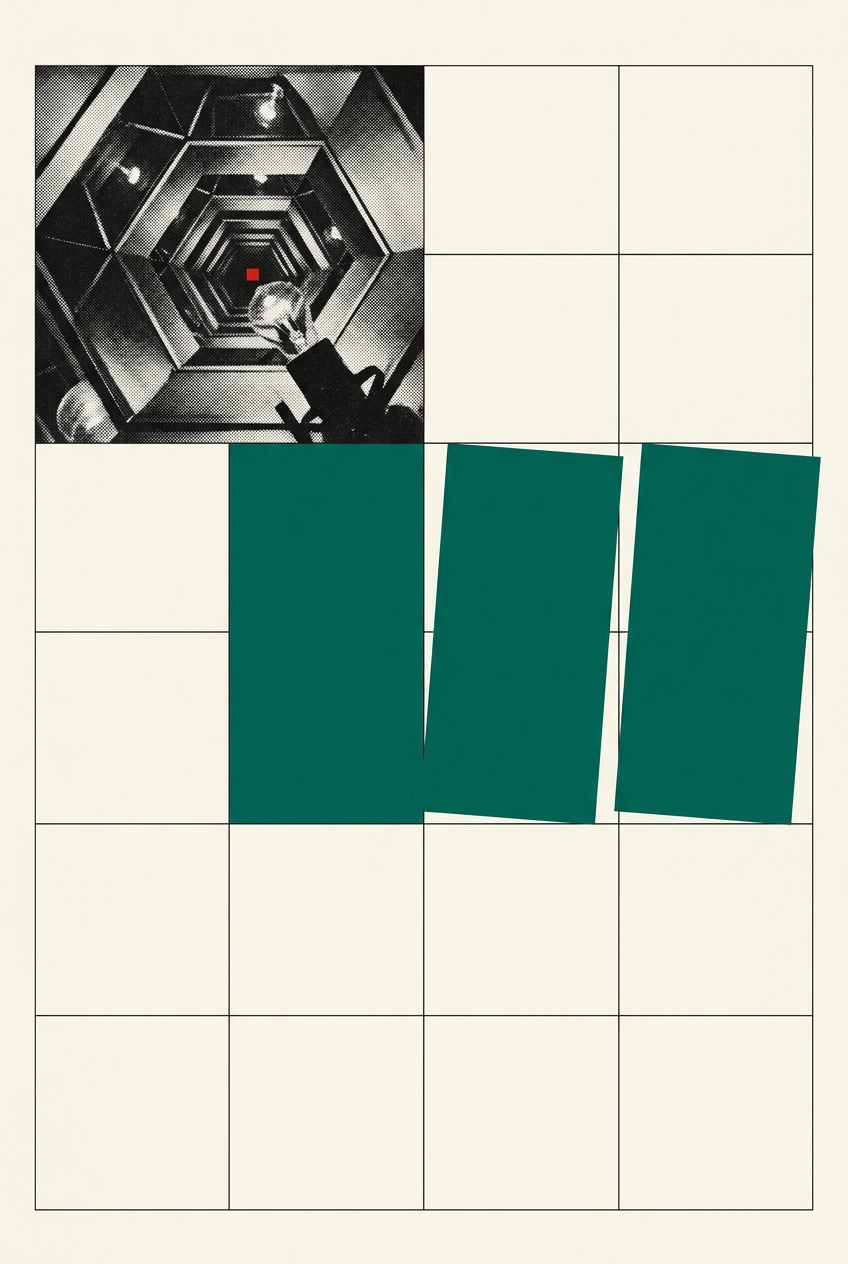
\includegraphics[width=\linewidth,height=0.92in,keepaspectratio]{plates/swiss/landmark-01.jpg}}%
    }{%
      \PackageError{pd-book-contents}{Missing chapter plate \pd@tocplatepath}%
        {Restore the chapter's edition-specific plate before building the Book.}%
    }%
  }}
% A fresh page for a part keeps its existing art and the first chapter together.
% The image is a visual locator for the same part plate encountered in the body.
\renewcommand*\l@part[2]{%
  \ifnum\pd@tocpart=0
    \par\addvspace{24pt}%
  \else
    \ifnum\pd@tocpart>\pdpartcount
      \Needspace*{14\baselineskip}\addvspace{24pt}%
    \else\clearpage\fi
  \fi
  \advance\pd@tocpart\@ne
  \pd@tocafterparttrue
  \ifnum\pd@tocpart>\pdpartcount
    \def\pd@toccolor{hhink}%
    {\pdtextface\LARGE\bfseries #1\hfill #2\par}%
    \vspace{9pt}\noindent\rule{\linewidth}{0.7pt}\par\vspace{12pt}%
  \else
    \edef\pd@toccolor{\csname pd@tocpartcolor@\the\pd@tocpart\endcsname}%
    \noindent
    \begin{minipage}[t]{0.29\linewidth}\vspace{0pt}%
      \expandafter\pd@tocplate\expandafter{\csname pd@tocpartart@\the\pd@tocpart\endcsname}%
    \end{minipage}\hfill
    \begin{minipage}[t]{0.66\linewidth}\vspace{0pt}\pdtextface\raggedright
      {\Large\bfseries\color{\pd@toccolor}#1\par}%
      \vspace{7pt}%
      {\small\csname pd@tocpartblurb@\the\pd@tocpart\endcsname\par}%
      \vspace{7pt}{\small Part opens on page #2\par}%
    \end{minipage}\par
    \vspace{13pt}\noindent{\color{\pd@toccolor}\rule{\linewidth}{1.1pt}}\par\vspace{10pt}%
  \fi\nobreak}
\newcommand*\l@chapter[2]{%
  \ifnum\pd@tocpart=0
    \Needspace*{15\baselineskip}\addvspace{22pt}%
    \noindent\begin{minipage}[t]{0.23\linewidth}\vspace{0pt}%
      \expandafter\pd@tocchapterplate\expandafter{\csname pd@tocchapterart@0\endcsname}%
    \end{minipage}\hfill
    \begin{minipage}[t]{0.72\linewidth}\vspace{0pt}%
    \begingroup
      \pdtextface\large\bfseries\color{\pd@toccolor}%
      \parindent\z@\rightskip 2.5em\parfillskip -2.5em
      \let\numberline\pd@tocchapternumber
      #1\nobreak\hfill\makebox[2.5em][r]{#2}\par
    \endgroup\nobreak
    \vspace{5pt}%
    {\rmfamily\small\raggedright
      \csname pd@tocchapterclaim@0\endcsname\par
      \edef\pd@tocnotename{pd@tocchapternote@0}%
      \expandafter\ifx\csname\pd@tocnotename\endcsname\@empty\else
        \vspace{3pt}{\itshape\csname\pd@tocnotename\endcsname\par}%
      \fi}%
    \end{minipage}\par\nobreak\vspace{10pt}%
  \else
    \ifpd@tocafterpart\pd@tocafterpartfalse\else
      \Needspace*{15\baselineskip}\addvspace{22pt}%
    \fi
    \advance\pd@tocchapter\@ne
    \noindent\begin{minipage}[t]{0.23\linewidth}\vspace{0pt}%
      \expandafter\pd@tocchapterplate\expandafter{\csname pd@tocchapterart@\the\pd@tocchapter\endcsname}%
    \end{minipage}\hfill
    \begin{minipage}[t]{0.72\linewidth}\vspace{0pt}%
    \begingroup
      \pdtextface\large\bfseries\color{\pd@toccolor}%
      \parindent\z@\rightskip 2.5em\parfillskip -2.5em
      \let\numberline\pd@tocchapternumber
      #1\nobreak\hfill\makebox[2.5em][r]{#2}\par
    \endgroup\nobreak
    \vspace{5pt}%
    {\rmfamily\small\raggedright
      \csname pd@tocchapterclaim@\the\pd@tocchapter\endcsname\par
      \edef\pd@tocnotename{pd@tocchapternote@\the\pd@tocchapter}%
      \expandafter\ifx\csname\pd@tocnotename\endcsname\@empty\else
        \vspace{3pt}{\itshape\csname\pd@tocnotename\endcsname\par}%
      \fi}%
    \end{minipage}\par\nobreak\vspace{10pt}%
  \fi}
\newcommand{\pd@tocchapternumber}[1]{#1\enspace}
% A quiet number gutter and one aligned page column. Subsections indent only
% their numbers; long titles keep a generous measure and wrap as hanging text.
\renewcommand*\l@section[2]{%
  \addvspace{5pt}\begingroup\pdtextface\normalsize\bfseries
    \@dottedtocline{1}{0pt}{3.8em}{#1}{#2}%
  \endgroup\nobreak}
\renewcommand*\l@subsection[2]{%
  \begingroup\pdtextface\small
    \@dottedtocline{2}{1.2em}{4.4em}{#1}{#2}%
  \endgroup}
\renewcommand*\l@subsubsection[2]{%
  \begingroup\color{hhgray}\pdcaptionface\footnotesize
    \@dottedtocline{3}{2.4em}{5em}{#1}{#2}%
  \endgroup}
\newcommand{\pdtableofcontents}{%
  \clearpage
  \newgeometry{inner=0.8in,outer=0.2in,top=0.85in,bottom=0.95in}%
  \begingroup
    \rmfamily\normalsize\color{hhink}%
    \parindent\z@\parskip\z@
    % Frontmatter roman folios need more room than the class's 1.55em gutter.
    \renewcommand\@pnumwidth{2.8em}\renewcommand\@tocrmarg{3.8em}%
    \setlength{\headwidth}{\textwidth}%
    \fancyhf{}\fancyhead[LE,RO]{\rmfamily\small Contents}%
    \fancyfoot[LE,RO]{\rmfamily\small\thepage}%
    \hypersetup{linkcolor=hhink}%
    \pd@tocpart=0 \pd@tocchapter=0 \pd@tocafterpartfalse
    \phantomsection\label{book:contents}%
    \pdfbookmark[0]{Contents}{book.contents}%
    {\pddisplayface\Huge\bfseries Contents\par}%
    \vspace{10pt}\noindent\rule{\linewidth}{1.1pt}\par\vspace{14pt}%
    {\pdtextface\large The complete argument, in \pdchaptercount{} chapters.\par}%
    \vspace{6pt}%
    \begin{minipage}{0.84\linewidth}\rmfamily\normalsize\raggedright
      Every chapter, section and subsection is listed here, followed by
      solutions, the result atlas, reference material and image credits.
      Titles and page numbers lead directly to their place in the book.
    \end{minipage}\par\vspace{20pt}%
    \@starttoc{toc}%
    \clearpage
  \endgroup
  \restoregeometry
}
\makeatother

% Hyperlink and cross-reference discipline (must stay last).
% Shared hyperlink and cross-reference discipline for the Book and its chapters.
% Load this LAST in every preamble: cleveref must follow hyperref and amsthm.
% hyperref itself is loaded earlier with [backref=page] (a load-time option).
% Twin copy under whitepaper/figures/ (byte-identical; checked by
% scripts/generate-mega-whitepaper.test.mjs).
%
% What a reader gets: live links on chapter titles, section numbers, theorems,
% figures, tables, equations, page numbers, and citations; PDF bookmarks three
% levels deep; and, at the end of every bibliography entry, the pages that cite it.
% Links are quiet: a warm dark ink one step lighter than body text, so the
% four part hues keep their meaning and an inline chapter title never competes
% with the part it sits in. Chrome pages (the front-matter map, part openers)
% recolor their own links locally.
\hypersetup{
  colorlinks=true,
  linkcolor=pdinkmuted,
  citecolor=pdinkmuted,
  urlcolor=pdinkmuted,
  filecolor=pdinkmuted,
  anchorcolor=pdink,
  bookmarksnumbered=true,
  bookmarksdepth=3,
  bookmarksopen=true,
  bookmarksopenlevel=1,
  breaklinks=true,
  linktoc=all,
  pdfauthor={Erich Owens},
  pdftitle={\pdchaptertitle},
  pdfsubject={\pdeditiontitle: \pdeditionsubtitle},
}

% Title-based chapter references. \pdchaplink{prefix}{text} is a live link to
% the chapter inside the Book (the Book's preamble defines it before loading this
% file); in a standalone chapter it is plain text. Prose uses \pdchapref, which
% sets the title in italics; the locator map uses \pdchaplink directly.
\providecommand{\pdchaplink}[2]{#2}
\DeclareRobustCommand{\pdchapref}[2]{\pdchaplink{#1}{\emph{#2}}}

% \ifpdbook -- true in the assembled Book, false otherwise.
%
% WHY THIS EXISTED. A drawing that two chapters both \input prints twice in the
% Book, under two figure numbers. The fix is for the chapter that develops the
% idea to keep the figure and the other to point at it -- but the standalone
% edition of a chapter had nowhere to point, and rewriting the prose outright
% removed five figures from harbor-economy-whitepaper.pdf and left it telling a
% conference reader that a ceremony is "drawn in The Federated Harbor", a
% document that reader did not have.
%
% WHERE IT STANDS NOW. The per-chapter PDFs are retired: the Book is the one
% document, so \ifpdbook is true in every build that renders, and the \else
% branches are source with no output. They are still here, and still read by
% check_duplicate_figures.py (which must not count an \else \input as a Book
% input) -- but nothing prints them, and nothing new should be put in one.
% Whether to delete them is an open question; see the retirement PR.
%
% The divergence was per-build. A CONDITIONAL and not a two-argument macro:
% the generator inlines each \input, so a figure branch is a whole table or
% tikzpicture, and as a macro argument that is scanned as one token list --
% which is how \pdinbook produced "runaway argument" on the first attempt.
% \ifpdbook skips the untaken branch at the TeX level instead.
%
% Declared unconditionally and defaulting FALSE, which is the standalone
% answer. The Book's preamble sets \pdbooktrue immediately after loading
% this file. A guard here would have to mention \ifpdbook or \newif inside a
% branch TeX may skip, and a conditional token in skipped text is counted as
% a nested \if -- which is how two attempts at a guard both produced
% "Incomplete \ifdefined". Ordering is cheaper than cleverness.
\newif\ifpdbook

% cleveref: "Theorem 3.1", "Figure 2.4", "Section 1.3", capitalised, never
% abbreviated, with the whole phrase clickable. Names are declared explicitly
% because the theorem environments are created before this file is loaded.
\usepackage[nameinlink,capitalise,noabbrev]{cleveref}
\crefname{pdchapter}{Chapter}{Chapters}
\crefname{part}{Part}{Parts}
\crefname{appendix}{Appendix}{Appendices}
\crefname{definition}{Definition}{Definitions}
\crefname{theorem}{Theorem}{Theorems}
\crefname{lemma}{Lemma}{Lemmas}
\crefname{proposition}{Proposition}{Propositions}
\crefname{corollary}{Corollary}{Corollaries}
\crefname{conjecture}{Conjecture}{Conjectures}
\crefname{property}{Property}{Properties}
\crefname{protocol}{Protocol}{Protocols}
\crefname{lsprotocol}{Protocol}{Protocols}
\crefname{stpprotocol}{Protocol}{Protocols}
\crefname{heprotocol}{Protocol}{Protocols}
\crefname{remark}{Remark}{Remarks}
\crefname{lstlisting}{Listing}{Listings}
\crefname{exercise}{Exercise}{Exercises}
\crefname{solution}{Solution}{Solutions}
\Crefname{pdchapter}{Chapter}{Chapters}
\Crefname{lstlisting}{Listing}{Listings}
\Crefname{exercise}{Exercise}{Exercises}
\Crefname{solution}{Solution}{Solutions}

% Back-references: "^ Cited on pages 12, 40, and 87." after every bibliography
% entry, each page number a live link back to the page that cited the work.
% Distinct pages only (#3/#4).
%
% The page numbers used to be wrapped in \color{hhgray} along with the words,
% which painted over the link colour hyperref had just given them: the links
% were there -- 29 annotations on a typical bibliography page -- and looked
% exactly like the grey prose around them, so nobody knew they could click.
% Restoring the quiet link colour would not have fixed it either; pdinkmuted
% against hhgray is 1.53:1, which is no signal at footnote size.
%
% So the numbers take pdcobalt (7.55:1 on the cream, and a hue a reader cannot
% mistake for grey), and the line opens with the return arrow this book already
% uses to send a solution back to its exercise. This is a deliberate exception
% to the quiet-link discipline above, and the reason is that back-matter
% navigation is the one place where the link IS the content: in prose the
% surrounding sentence tells you a phrase is a destination, and in a
% bibliography nothing does.
\renewcommand*{\backref}[1]{}
\renewcommand*{\backrefalt}[4]{%
  \ifcase #3\relax
  \or {\footnotesize{\color{hhgray}$\uparrow$~Cited on page}~{\hypersetup{linkcolor=pdcobalt}#4}{\color{hhgray}.}}%
  \else {\footnotesize{\color{hhgray}$\uparrow$~Cited on pages}~{\hypersetup{linkcolor=pdcobalt}#4}{\color{hhgray}.}}%
  \fi}
\renewcommand*{\backrefsep}{, }
\renewcommand*{\backreftwosep}{ and }
\renewcommand*{\backreflastsep}{, and }

% \ifpdbook is declared (false) in pd-hyperlinks; the Book turns it on here,
% AFTER the load, so nothing has to guard the \newif. It selects the Book
% branch wherever a chapter and its standalone paper must diverge -- a
% figure the Book prints once and cross-references, which the paper carries
% its own copy of.
\pdbooktrue

% ---------------------------------------------------------------------------
% Captioned exhibits must fit the text column: the outside margin is reserved
% for their captions. Record true ink width and warn on overflow; the matching
% PDF audit rejects it. Never hide an oversized figure by shrinking its type
% or moving its caption below it. The legacy spill/scale path below applies
% only to non-floating inline artwork and remains separately reviewable.
% ---------------------------------------------------------------------------
\usepackage{changepage}
\strictpagecheck
\newlength{\pdfullwidth}\setlength{\pdfullwidth}{\dimexpr\textwidth+\marginparsep+\marginparwidth\relax}
\makeatletter
% pgf hands every finished picture (tikzpicture, pgfplots axis, inline \tikz)
% to \pgfsys@typesetpicturebox with its width known; the hook decides where it
% goes. Nested pictures pass through untouched (their box is narrower than the
% line they sit in).
\newsavebox{\pd@picbox}
\let\pd@typesetpicturebox\pgfsys@typesetpicturebox
\def\pgfsys@typesetpicturebox#1{%
  \sbox{\pd@picbox}{\pd@typesetpicturebox#1}%
  % Figure-band recording for \pd@placemargin's centering (pd-pedagogy.tex):
  % from THIS box's own \ht/\dp, not from \pagetotal at \end{figure}. The
  % latter was tried first and does not work -- for an [H] float the
  % package defers inserting the box into the main vertical list past
  % \end{figure} itself, so \pagetotal read there (even settled) still
  % under-reads by the whole figure and \pd@figbot came out equal to
  % \pd@figtop on every figure measured. \pagetotal HERE, mid-paragraph
  % while pgf is still handing us the finished picture box, is the page
  % height immediately above where this box is about to be placed, and the
  % box's own \ht+\dp is its true rendered height regardless of how (or
  % whether) it gets rescaled below -- both read before any resizing, which
  % is fine: \pd@placemargin only wants the figure's vertical band, and
  % \resizebox below does not change a box's VERTICAL position, only its
  % size, and \centering does not move a box vertically at all.
  \ifpdmargincolumn
    \xdef\pd@figpage{\number\value{page}}%
    \global\pd@figtop=\pagetotal
    \global\pd@figbot=\dimexpr\pagetotal+\ht\pd@picbox+\dp\pd@picbox\relax
  \fi
  % the box has no width of its own yet; pgf sets it from the bounding box
  \@tempdima=\dimexpr\pgf@picmaxx-\pgf@picminx\relax
  \ifpd@captionfloat
    \ifdim\@tempdima>\pd@exhibitinkwidth
      \global\pd@exhibitinkwidth=\@tempdima\fi
  \fi
  \ifdim\@tempdima>\dimexpr\linewidth+1pt\relax
    \ifpd@captionfloat
      % The outer margin belongs to the caption. Preserve the bad geometry
      % for the audit; never conceal it by shrinking type or dropping captions.
      \PackageWarning{pd-book}{PD-EXHIBIT-WIDE: \@captype\space
        \@nameuse{the\@captype}; width=\the\@tempdima; limit=\the\linewidth}%
      \makebox[\linewidth][c]{\usebox{\pd@picbox}}%
    \else
    \ifdim\linewidth<\dimexpr\textwidth-1pt\relax
      \ifpdmarginevidence
        \PackageError{pd-book}{Margin evidence exceeds its native width}%
          {Redraw to marginparwidth; shrinking labels is not permitted.}%
        \usebox{\pd@picbox}%
      \else
      % inside a minipage, a margin note or a table cell: fit the box we are in
      \PackageWarning{pd-book}{picture \the\wd\pd@picbox\space wide scaled to a \the\linewidth\space box}%
      \resizebox{\linewidth}{!}{\usebox{\pd@picbox}}%
      \fi
    \else
      \ifdim\wd\pd@picbox>\pdfullwidth
        \PackageWarning{pd-book}{picture \the\wd\pd@picbox\space wide scaled to the full width}%
        \sbox{\pd@picbox}{\resizebox{\pdfullwidth}{!}{\usebox{\pd@picbox}}}%
      \else
        \PackageInfo{pd-book}{picture \the\wd\pd@picbox\space wide set full width}%
      \fi
      % Strict page checking records the box's shipped page in the aux file,
      % so a floated picture uses its physical leaf rather than the page TeX
      % happened to be composing when the hook fired. Odd rectos spill right;
      % even versos spill left. The text measure never shrinks to make room.
      \checkoddpage
      \ifoddpage
        \makebox[\textwidth][l]{\usebox{\pd@picbox}}%
      \else
        \makebox[\textwidth][r]{\usebox{\pd@picbox}}%
      \fi
    \fi
    \fi
  \else
    \usebox{\pd@picbox}%
  \fi}
\NewDocumentCommand\pdpagecentered{O{\pdfullwidth} m}{%
  \par\noindent\checkoddpage
  \makebox[\textwidth][c]{%
    \ifoddpage\hspace*{0.45in}\else\hspace*{-0.45in}\fi
    \makebox[#1][c]{#2}%
  }\par
}
\NewDocumentCommand\pdpagecaption{O{} m O{}}{%
  \par\vspace{6pt}%
  \begingroup
  \let\pd@captiontype\relax
  \pd@routecaptionfalse
  \noindent\checkoddpage
  \makebox[\textwidth][c]{%
    \ifoddpage\hspace*{0.45in}\else\hspace*{-0.45in}\fi
    \begin{minipage}{\dimexpr\pdfullwidth-0.2in\relax}%
      \if\relax\detokenize{#1}\relax\caption{#2}\else\caption[#1]{#2}\fi
      \if\relax\detokenize{#3}\relax\else\label{#3}\fi
    \end{minipage}%
  }%
  \endgroup
  \par
}
\NewDocumentCommand\pdwidecaption{O{} m O{}}{%
  \pdpagecaption[#1]{#2}[#3]%
}
\makeatother

% Book-owned openings and handoffs. The chapter sources remain independently
% buildable; these rails exist only in the Book. They are keyed by chapter
% prefix (see whitepaper/textbook.json), never by position, so reordering the
% book moves a chapter's rails with it. The handoff text, however, is written
% for the order the book is in: it names the chapter that comes next.
%
% An opening rail sits at the top of a chapter's first body page. Its heading
% is the chapter's question (from textbook.json, the same line the opener page
% set large); its body is the lede: the scene, in two or three sentences,
% before the chapter's own first section begins.

\newcommand{\pdbookrail}[2]{%
  \par\vspace{0.5cm}%
  \noindent{\color{\pdcurrentchaptercolor}\rule{2.5em}{1.5pt}}\par
  \vspace{0.12cm}%
  \noindent{\small\scshape\bfseries\color{hhink}#1}\enspace
  {\small #2}\par
  \vspace{0.45cm}%
}

% ---- Part I: The Machine -------------------------------------------------

\newcommand{\pdchapteropeningswk}{%
  \pdbookrail{\pdchapterquestion}{%
    Six agents may agree about a file and still overwrite one another. A log can
    report the collision after the fact; only a mediated writer can refuse the
    second effect before it lands. This chapter identifies that local writer,
    separates preventable rules from detect-only claims, and states the work-unit
    invariants that every later institution assumes. R5 and R8 set the boundary.}%
}

\newcommand{\pdchapterhandoffswk}{%
  \pdbookrail{What \pdchapref{anchor}{The Anchor Protocol} receives}{%
    Local effects now have one serial history, one fencing epoch, and one place
    to attach receipts. The writer decides what becomes real; it does not yet say
    who may ask it to. The next chapter turns authority into a key-bound,
    attenuating, revocable object, so that every request the kernel admits
    arrives with a checked pedigree.}%
}

\newcommand{\pdchapteropeninganchor}{%
  \pdbookrail{\pdchapterquestion}{%
    Identity answers who signed; it does not answer what the signer may do.
    Anchor therefore checks every delegation edge, binds the grant to a key and
    audience, narrows scope and lifetime, and preserves revocation ancestry.
    The formal claim concerns the checked protocol and Rust paths, while R5
    explains which surrounding policy promises can become admission gates.}%
}

\newcommand{\pdchapterhandoffanchor}{%
  \pdbookrail{What \pdchapref{sealed}{The Sealed Harbor} receives}{%
    A request now arrives with authenticated, narrowing authority, and the kernel
    that admits it keeps one durable history. Some work needs more than an
    authorized writer: it needs a room in which two parties who trust neither
    each other nor the venue can still get one answer out. The next chapter
    builds that room and prices what can leave it through the slot.}%
}

\newcommand{\pdchapteropeningsealed}{%
  \pdbookrail{\pdchapterquestion}{%
    A proprietary model and a proprietary dataset must produce one answer that
    neither owner will let the other see. The kernel refuses a write it has not
    authorized and the Anchor checks who asked; neither says what may leave a
    room through the only slot in its wall. This chapter builds the sealed room:
    one work order, two fences, two gates, and four properties, each stated at
    the strength its check earns. R9, R10, and R11 govern its strongest claims.}%
}

\newcommand{\pdchapterhandoffsealed}{%
  \pdbookrail{What \pdchapref{ls}{The Legible Swarm} receives}{%
    The machine now has three parts that can be kept honest: a writer with
    one history, an authority that arrives checked, and a room whose only exit
    is metered. Notice what the third part cost. Sealing execution so that a
    secret cannot walk out is the same act as making the inside of the
    computation dark to the person responsible for it --- the slot is the only
    place anyone sees through the wall, and \S3.7 metered exactly what leaves
    it. Part~I therefore ends holding an operator who is accountable for work
    it can no longer watch directly. That is not a philosophical turn, it is
    the bill for the room, and the next chapter is the reply to it: with many
    such machines running at once, what must remain visible to the operator,
    and what does reading it cost?}%
}

% ---- Part II: The Operator -----------------------------------------------

\newcommand{\pdchapteropeningls}{%
  \pdbookrail{\pdchapterquestion}{%
    The previous chapter sealed the room and, in the same stroke, put the work
    beyond the operator's sight; this chapter is the information-theoretic
    answer to that darkness. A swarm can produce more events than its operator
    can read. The resulting
    scarcity is not cured by a smoother summary: some summaries make the
    decisive artifact unreachable. This chapter establishes the cost of a
    zero-miss digest, proves why a successor and an operator require different
    rankings, and derives the attention rule from explicit error costs. Its
    strongest claims are governed by R1--R4, R14, and R16.}%
}

\newcommand{\pdchapterhandoffls}{%
  \pdbookrail{What \pdchapref{stp}{From Spawn to Person} receives}{%
    The operator now has a disciplined read surface: claims remain linked to
    artifacts, attention is priced, and uncertainty is visible. A process can
    still die, restart under a new model, or shed its local memory. The next
    chapter asks what must persist so yesterday's act can still be attributed
    tomorrow.}%
}

% ---- Part III: The Person ------------------------------------------------

\newcommand{\pdchapteropeningstp}{%
  \pdbookrail{\pdchapterquestion}{%
    Accountability cannot attach to a disposable process name. It needs a
    durable identity, a named principal, an outcome history, and rules for
    migration that do not erase sanctions or mint reputation. This chapter
    builds that continuity without pretending software has a human soul. R12,
    R13, and B6 govern its economic and protocol claims.}%
}

\newcommand{\pdchapterhandoffstp}{%
  \pdbookrail{What \pdchapref{he}{The Harbor Economy} receives}{%
    A successor can now inherit a bounded history without inheriting imaginary
    credit or escaping old obligations. Continuity by itself creates no market:
    it neither prices risk nor says whose funds may move. The next chapter turns
    attributed work into exchange by separating value, collateral, evidence,
    and settlement.}%
}

% ---- Part IV: The Market -------------------------------------------------

\newcommand{\pdchapteropeninghe}{%
  \pdbookrail{\pdchapterquestion}{%
    A payment rail moves money; a market must also identify the parties, state
    what performance means, reserve the right funds, and decide what happens
    when evidence disagrees. This chapter constructs that market from four
    separate monetary buckets and explicit oracles. R7 and R13--R15 delimit the
    audit, substitution, escalation, and specialization claims.}%
}

\newcommand{\pdchapterhandoffhe}{%
  \pdbookrail{What \pdchapref{bonded}{The Bonded Commons} receives}{%
    Work can now be proposed, bonded, graded, and settled against a named
    principal. The market's contracts rest on promises this chapter states but
    does not prove: that evidence is admissible, that settlement conserves value,
    that remedy stays bounded. The next chapter proves them.}%
}

\newcommand{\pdchapteropeningbonded}{%
  \pdbookrail{\pdchapterquestion}{%
    Attribution without consequence is only a diary; consequence without
    admissible evidence is arbitrary. This chapter turns the local writer into
    an institution by joining capability bounds, witnessed records, audits,
    appeals, and conserved settlement. R7--R11, R15, R17, and the R8 machine
    state exactly what has been proved, checked, or left conditional.}%
}

\newcommand{\pdchapterhandoffbonded}{%
  \pdbookrail{What \pdchapref{fh}{The Federated Harbor} receives}{%
    One machine can now authorize, observe, adjudicate, and settle its own work.
    A second machine introduces a different operator and a different source of
    truth. The final chapter asks which capabilities and records may cross that
    boundary without pretending that either local authority has become global.}%
}

\newcommand{\pdchapteropeningfh}{%
  \pdbookrail{\pdchapterquestion}{%
    The current Relay federates harbor-scoped events over outbound HTTPS and
    SSE; it does not replicate daemon state or create consensus between
    operators. Local admission remains local. The research result is narrower
    and sharper still: R6 and CR-1/2/3 show exactly when relayed reports around a
    cycle can expose an inconsistency that a missing pairwise check cannot.}%
}

\newcommand{\pdchapterhandofffh}{%
  \pdbookrail{The conclusion of the book}{%
    The seven answers now form one discipline. Mediate every effect that must be
    prevented; let delegated authority only narrow; preserve enough evidence for
    a human to challenge the system; attach actions to a durable principal and
    work unit; make settlement conserve value; and cross organizational
    boundaries by exchanging verifiable records rather than by exporting
    sovereignty. Better models help inside this discipline. They do not replace
    it.}%
}

% References belong beside the discussion throughout the assembled Book.
% The registry remains build data; standalone chapter behavior is unchanged.
\providecommand{\pdEnableMarginCitations}{1}
\ifdefined\pdEnableMarginCitations
  % Book-only citations. Load AFTER pd-margin-layout, before document.
% No bibliography is printed; the source registry remains reproducible data.
% Enabled by default in the assembled Book; standalone chapters are unchanged.
% Public references are unnumbered. Registry integers are accounting data,
% never superscript callouts or bold numerals in the reader's margin.
\makeatletter
\newif\ifpdbookinmargin
\newif\ifpdbookcitereplay
\newcommand{\pdbookmargincontext}[1]{\begingroup\pdbookinmargintrue #1\endgroup}
\NewCommandCopy\pdbookoriginalmarginregister\pdmarginregister
\RenewDocumentCommand\pdmarginregister{m +m}{%
  \pdbookoriginalmarginregister{#1}{\pdbookmargincontext{#2}}}
% Captions/portraits/exhibits are measured BEFORE they reach the allocator.
% Mark that earlier measurement too: a citation belongs to its owning box.
\let\pdbookoriginalstorecaption\pd@storecaption
\renewcommand{\pd@storecaption}[1]{%
  \pdbookmargincontext{\pdbookoriginalstorecaption{#1}}}
\let\pdbookoriginalmarginfigure\pdmarginfigure
\renewcommand{\pdmarginfigure}[2]{%
  \pdbookmargincontext{\pdbookoriginalmarginfigure{#1}{#2}}}
\NewCommandCopy\pdbookoriginalmarginexhibit\pdmarginexhibit
\RenewDocumentCommand\pdmarginexhibit{m m +m +m}{%
  \pdbookmargincontext{\pdbookoriginalmarginexhibit{#1}{#2}{#3}{#4}}}
% A contents/figure-list replay must not consume first use or emit a note.
\let\pdbookoriginalstarttoc\@starttoc
\renewcommand{\@starttoc}[1]{%
  \begingroup\pdbookcitereplaytrue\pdbookoriginalstarttoc{#1}\endgroup}
% tabularx evaluates its body several times while finding column widths.
% Its trial argument runs INSIDE the discarded trial box, so this flag is
% local to measurement and cannot consume first use or register ghost notes.
% https://github.com/latex3/latex2e/blob/develop/required/tools/tabularx.dtx
\let\pdbookoriginalTXtrial\TX@trial
\def\TX@trial#1{\pdbookoriginalTXtrial{\pdbookcitereplaytrue #1}}
\providecommand{\pdbookcitationrecord}[4]{}
\ExplSyntaxOn
\prop_new:N \g_pd_book_cite_number_prop
\prop_new:N \g_pd_book_cite_full_prop
\prop_new:N \g_pd_book_cite_short_prop
\prop_new:N \g_pd_book_cite_seen_prop
\prop_new:N \g_pd_book_cite_page_prop
\int_new:N \g_pd_book_cite_occurrence_int
\tl_new:N \l_pd_book_cite_page_tl
\clist_new:N \l_pd_book_cite_fresh_clist
\bool_new:N \l_pd_book_cite_first_bool
\cs_new_protected:Npn \pd_book_cite_require:n #1
  {\prop_if_in:NnF \g_pd_book_cite_number_prop {#1}
    {\PackageError{pd-book-citations}{Unregistered~source:~#1}
      {Register~the~source.~Never~silently~drop~a~citation.}}}
\NewDocumentCommand\pdbookreference{m m +m +m}
  {\prop_if_in:NnTF \g_pd_book_cite_number_prop {#1}
    {\PackageError{pd-book-citations}{Duplicate~source:~#1}
      {Use~one~canonical~entry~per~source.}}
    {\prop_gput:Nnn \g_pd_book_cite_number_prop {#1}{#2}
     \prop_gput:Nnn \g_pd_book_cite_full_prop {#1}{#3}
     \prop_gput:Nnn \g_pd_book_cite_short_prop {#1}{#4}}}
\cs_new_protected:Npn \pd_book_cite_entry:n #1
  {\pd_book_cite_require:n {#1}
   \par\noindent
   \prop_if_in:NnTF \g_pd_book_cite_seen_prop {#1}
    {\hyperlink{pdbook-source-#1}{\prop_item:Nn \g_pd_book_cite_short_prop {#1}}
     \iow_log:x {PD-BOOK-SOURCE:~key=#1,~form=repeat}}
    {\hypertarget{pdbook-source-#1}{}%
     \prop_item:Nn \g_pd_book_cite_full_prop {#1}
     \prop_gput:Nnn \g_pd_book_cite_seen_prop {#1}{1}
     \iow_log:x {PD-BOOK-SOURCE:~key=#1,~form=full}}}
\cs_new_protected:Npn \pd_book_cite_text:nn #1#2
  {\begingroup\mdseries\upshape
   \let\newblock\space
   \bool_set_true:N \l_pd_book_cite_first_bool
   \clist_map_inline:nn {#2}
     {\bool_if:NF \l_pd_book_cite_first_bool {\par\smallskip}
      \bool_set_false:N \l_pd_book_cite_first_bool
      \pd_book_cite_entry:n {##1}}
   \tl_if_blank:nF {#1}{\par\nobreak\emph{Cited:~#1.}}
   \par\endgroup}
\cs_new_protected:Npn \pd_book_cite_record:nnn #1#2#3
  {\int_gincr:N \g_pd_book_cite_occurrence_int
   \exp_args:Nx \zsavepos {pdc-\int_use:N\g_pd_book_cite_occurrence_int}
   \iow_log:x {PD-BOOK-CITE:~occurrence=\int_use:N\g_pd_book_cite_occurrence_int,
      ~keys=\tl_to_str:n{#2},~context=#3,~locator=\tl_to_str:n{#1}}
   \protected@write\@auxout{}
     {\string\pdbookcitationrecord{\int_use:N\g_pd_book_cite_occurrence_int}
       {#2}{#3}{\unexpanded{#1}}}}
% Repeated marks on the same physical page share one readable margin source.
% Use shipped positions from the prior pass, never the current page counter
% (which is wrong inside a paragraph or delayed float). Locators get their own
% note so consolidation cannot erase the specific passage being cited.
\cs_new_protected:Npn \pd_book_cite_note:nn #1#2
  {\tl_set:Nx \l_pd_book_cite_page_tl
    {\zref@extractdefault{pdc-\int_use:N\g_pd_book_cite_occurrence_int}{abspage}{0}}
   \clist_clear:N \l_pd_book_cite_fresh_clist
   \clist_map_inline:nn {#2}
    {\tl_set:Nx \l_tmpa_tl {\tl_use:N\l_pd_book_cite_page_tl / ##1}
     \bool_set_false:N \l_tmpa_bool
     \tl_if_eq:NnT \l_pd_book_cite_page_tl {0}{\bool_set_true:N\l_tmpa_bool}
     \tl_if_blank:nF {#1}{\bool_set_true:N\l_tmpa_bool}
     \prop_if_in:NVF \g_pd_book_cite_page_prop \l_tmpa_tl {\bool_set_true:N\l_tmpa_bool}
     \bool_if:NT \l_tmpa_bool
       {\clist_put_right:Nn \l_pd_book_cite_fresh_clist {##1}
        \prop_gput:NVn \g_pd_book_cite_page_prop \l_tmpa_tl {1}}}
   \clist_if_empty:NTF \l_pd_book_cite_fresh_clist
     {\pdmarginreserveslot
      \iow_log:x {PD-BOOK-CITE-SHARED:~occurrence=\int_use:N\g_pd_book_cite_occurrence_int}}
     {\exp_args:NnV \pd_book_cite_register:nn {#1}\l_pd_book_cite_fresh_clist}}
\cs_new_protected:Npn \pd_book_cite_register:nn #1#2
  {\pdmarginregister{citation}{\pd_book_cite_text:nn{#1}{#2}}
   \iow_log:x {PD-BOOK-CITE-BOX:~occurrence=\int_use:N\g_pd_book_cite_occurrence_int,
     ~id=\pdmarginlastid,~keys=\tl_to_str:n{#2}}}
\NewDocumentCommand\pdbookcite{O{} m}
  {\ifpdbookcitereplay
     \unskip
   \else
     \ifpdbookinmargin
       \pd_book_cite_record:nnn{#1}{#2}{embedded}%
       \par\smallskip\pd_book_cite_text:nn{#1}{#2}%
     \else
       % Existing sources use word~\cite{key}. Remove that obsolete gap so
       % punctuation does not acquire an extra space when the callout vanishes.
       \unskip
       \pd_book_cite_record:nnn{#1}{#2}{body}%
       \pd_book_cite_note:nn{#1}{#2}%
     \fi
   \fi}
\AtEndDocument{\iow_log:x {PD-BOOK-CITE-SUMMARY:~occurrences=
  \int_use:N\g_pd_book_cite_occurrence_int,~sources=
  \prop_count:N\g_pd_book_cite_seen_prop,~registered=
  \prop_count:N\g_pd_book_cite_number_prop}}
\ExplSyntaxOff
% An authored sidenote carries its own thought, not a displaced bibliography.
% Sources inside it are credited in the same measured box. No nested note,
% arbitrary public number or duplicate inline callout is created.
\RenewDocumentCommand\pdsourceaside{+m}{\pdmarginregister{aside}{#1}}
\AtBeginDocument{%
  \typeout{PD-BOOK-CITE-CAPACITY: \the\textheight}%
  \RenewDocumentCommand\pdcite{O{} m}{\pdbookcite[#1]{#2}}%
  \RenewDocumentCommand\cite{O{} m}{\pdbookcite[#1]{#2}}%
}
\makeatother

  \pdgeneratedinput{../../../.cache/whitepaper-build/coordination-papers-mega-volume/mega-volume-margin-references.tex}{margin references}
\fi
\hypersetup{
  pdftitle={\pdeditiontitle: \pdeditionsubtitle},
  pdfauthor={Erich Owens},
  pdfsubject={Eight chapters, in dependency order, on accountable autonomous work},
  pdfkeywords={supervisory control, multi-agent systems, capability security, coordination, accountability, federation}
}

\begin{document}
\hypersetup{pageanchor=false}
\begin{titlepage}
\pagecolor{hhpaper}\color{hhink}
\ifpdswiss
  % Swiss cover A (SWISS-BRIEF, C): the arcs block on the lower 56 per cent,
  % three type sizes on one left datum at 14 mm, the imprint in the foot.
  \pdswisscoverart
  \begin{tikzpicture}[remember picture,overlay,shift={(current page.north west)},x=1mm,y=-1mm]
    % The type block ends at about 28% of the 254mm page, which is the number
    % the cover plate's reserved band has to clear: see
    % scripts/whitepaper-plates/check_cover_title_band.py, which measures the
    % plate and fails the build rather than leaving it to the eye. Round 4a's
    % cover looked clean in a contact sheet, started its photograph 2% down,
    % and printed the subtitle over a container port.
    % All three lines live in the plate's reserved band, top-left, and the
    % image has the rest of the sheet. The imprint used to sit at the foot,
    % which put 9pt type over a halftone photograph that is 37% lighter than
    % luminance 140 -- neither black nor reversed white reads on that.
    \node[anchor=north west,inner sep=0pt,text width=145mm,align=left] at (14,14) {%
      {\pdcovergrotesk\fontsize{28}{33}\selectfont\bfseries\color{hhink}\spaceskip=0pt\xspaceskip=0pt%
       Governing AI Agents:\\[1.5mm]%
       The Harbor, the Person,\\and the Economy\par}%
      \vspace{5mm}%
      {\pdcovergrotesk\fontsize{11}{14}\selectfont\color{hhink}\spaceskip=0pt\xspaceskip=0pt%
       \pdeditionsubtitle\par}%
      \vspace{4mm}%
      {\pdcovergrotesk\fontsize{8.5}{11}\selectfont\color{hhgray}\spaceskip=0pt\xspaceskip=0pt%
       Erich Owens\quad\textperiodcentered\quad Curiositech\quad\textperiodcentered\quad Textbook Edition\par}%
    };
  \end{tikzpicture}
\else\ifpdtechnical
  % Technical cover: the engraving in the lower two thirds of the sheet, the
  % type in the paper above it, the sheet's frame and title block over all.
  \pdtechsheetplain{\pdeditiontitle}{Cover}%
  \begin{tikzpicture}[remember picture,overlay,shift={(current page.south west)},x=1in,y=1in]
    \IfFileExists{plates/technical/cover.jpg}{%
      \node[anchor=south,inner sep=0pt] at (3.5,1.55) {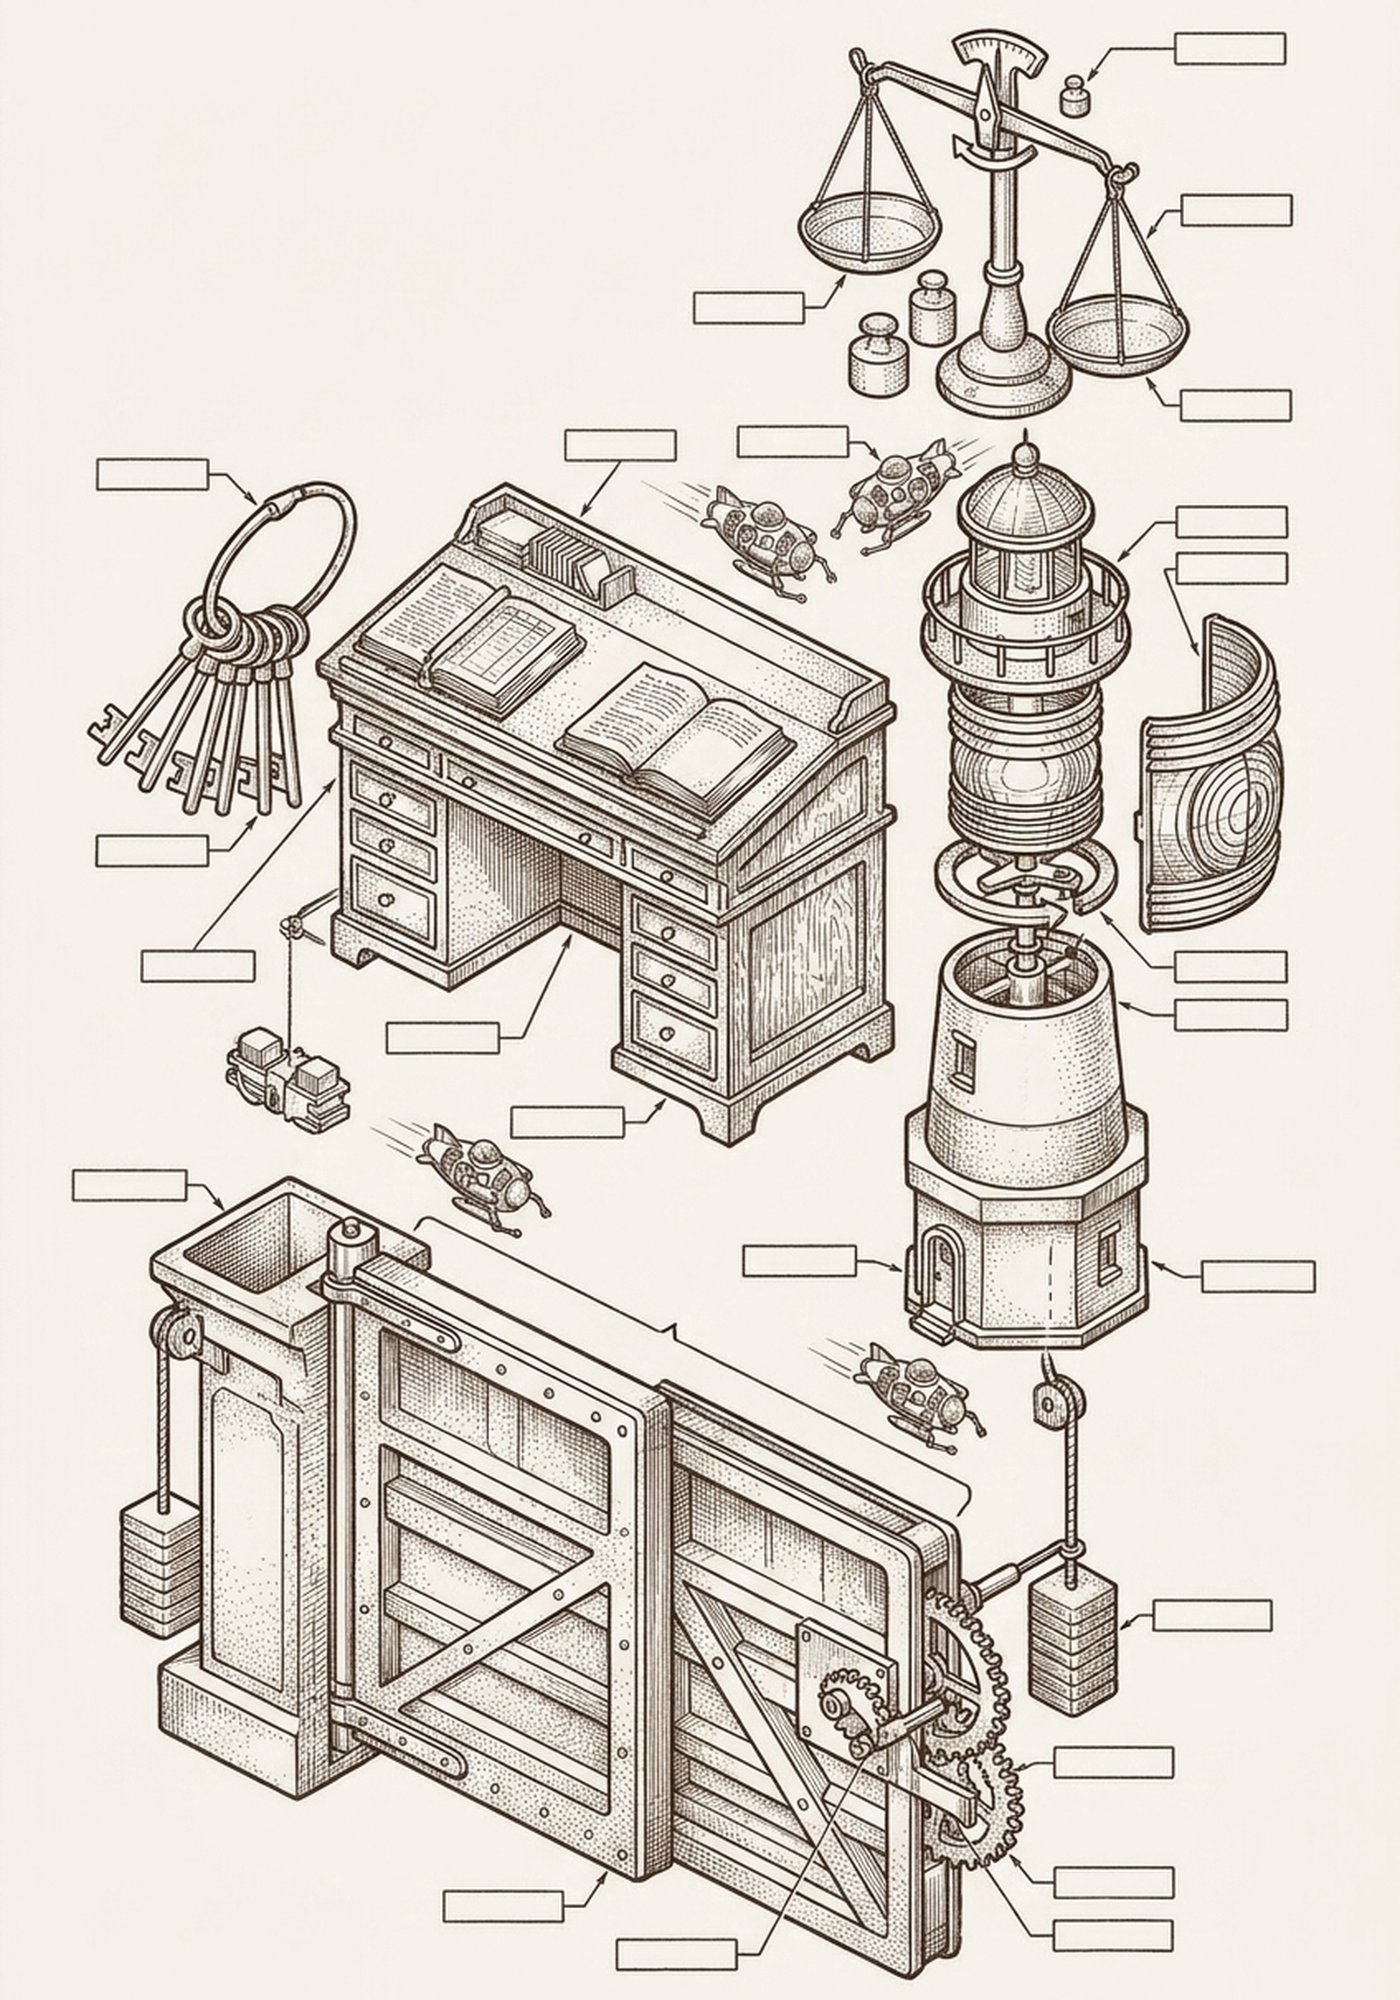
\includegraphics[height=4.55in]{plates/technical/cover.jpg}};}{}
    \node[anchor=north west,inner sep=0pt,text width=5.2in,align=left,font=\pdgrotesk\fontsize{24}{28}\selectfont,text=hhink] at (0.9,9.15) {\pdeditiontitle};
    \node[anchor=north west,inner sep=0pt,text width=5.2in,align=left,font=\pdgrotesk\fontsize{11}{14}\selectfont,text=hhink] at (0.9,7.8) {\pdeditionsubtitle};
    \node[anchor=north west,inner sep=0pt,font=\pdgrotesk\fontsize{9}{11}\selectfont,text=hhink] at (0.9,7.35) {Erich Owens\quad\textperiodcentered\quad Curiositech\quad\textperiodcentered\quad Textbook Edition};
  \end{tikzpicture}
\else
% Cover: the wash plate bleeds over the whole page; the type stays minimal and set in Times.
\IfFileExists{plates/jacket.jpg}{%
  \AddToShipoutPictureBG*{\AtPageLowerLeft{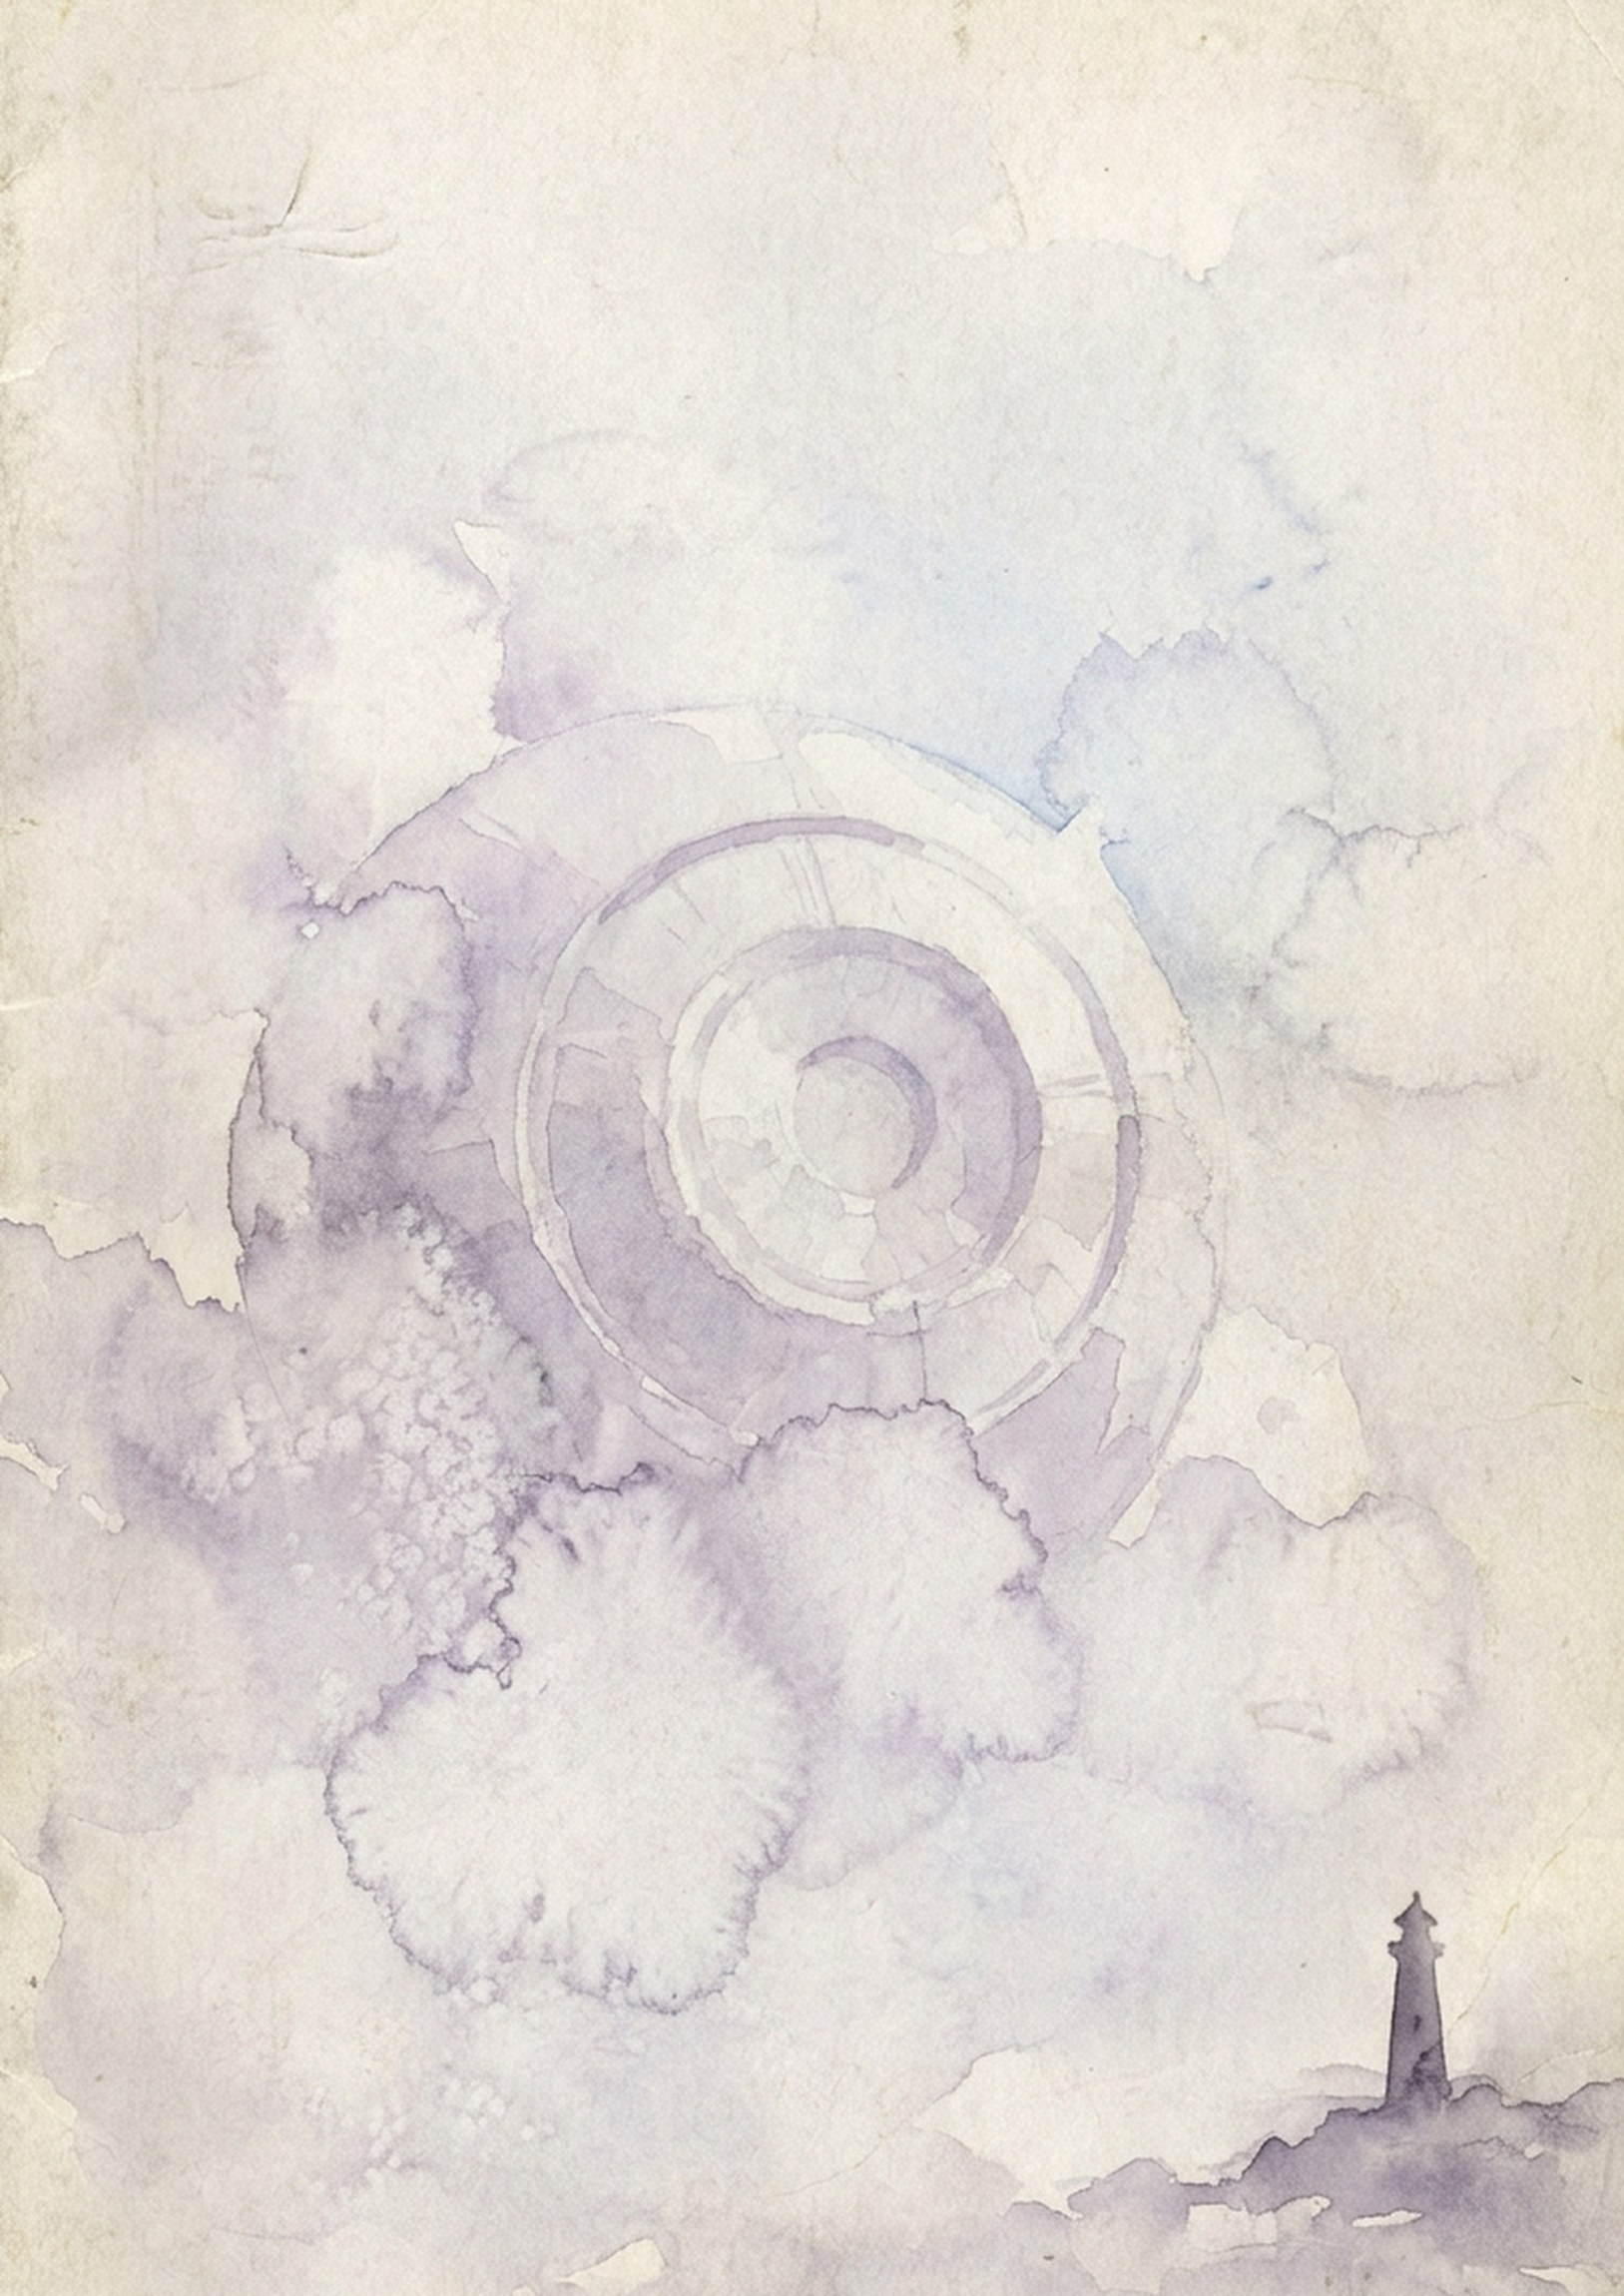
\includegraphics[width=\paperwidth,height=\paperheight]{plates/jacket.jpg}}}}{}%
\vspace*{1.2cm}
\noindent\begin{minipage}{0.88\textwidth}
{\pdpartface\fontsize{30}{36}\selectfont\raggedright Governing AI Agents:\\[2mm] The Harbor, the Person,\\ and the Economy\par}
\vspace{0.6cm}
\noindent{\color{pdcobalt}\rule{0.24\textwidth}{1pt}}\par
\vspace{0.45cm}
{\pdpartface\itshape\fontsize{14.5}{19}\selectfont \pdeditionsubtitle\par}
\end{minipage}
\vfill
\noindent{\pdpartface\scshape\small Erich Owens\par\vspace{3pt}Curiositech\ \textperiodcentered\ Textbook Edition\par}
\vspace*{0.4cm}
\fi\fi
\end{titlepage}
% Imprint page: the claim, the ordering rule, and the publication data that the cover no longer carries.
\clearpage\thispagestyle{empty}\pagecolor{hhpaper}\color{hhink}
\vspace*{\fill}
\noindent\pdweightrule{0}{\textwidth}{2.6pt}\par
\vspace{0.6cm}
\noindent\begin{minipage}{0.96\textwidth}\small
{\large\bfseries\pdeditiontitle}\par\vspace{3pt}
{\color{hhgray}\pdeditionsubtitle}\par\vspace{10pt}
{\bfseries\pdeditionclaim}\par\vspace{6pt}
{\color{hhgray}This book follows that claim from one machine and one operator to work shared
across principals, economic interests, and mutually distrustful systems. Its \pdchaptercountword{}
chapters are ordered by what they stand on; each proof chapter follows the chapter whose promises it
keeps.}\par\vspace{12pt}
Erich Owens \textperiodcentered\ Curiositech LLC \textperiodcentered\ \texttt{engineering@portdaddy.dev}\par
Curiositech \textperiodcentered\ Version \pdeditionversion\ \textperiodcentered\ \pdeditiondate\ \textperiodcentered\ \url{https://portdaddy.dev/whitepaper}\par
\end{minipage}
\vspace*{1.0cm}
\clearpage
% Frontispiece: the plate faces the title matter, in the edition's own register.
%
% It used to be one maritime etching printed in all three editions and wrapped
% in \IfFileExists, which is two defects in four lines. The etching's vellum and
% cross-hatching in front of the Swiss edition's flat colour blocks announced
% that the character stops at the cover; and a missing plate printed NOTHING, so
% the book would have shipped without a frontispiece and told nobody -- the
% silent fallback the plate rule exists to forbid (see the \PackageError in
% coordination-papers-mega-volume-swiss-plates.tex, which this now matches).
\newcommand{\pdfrontispiece}[1]{%
  \IfFileExists{#1}{%
    \thispagestyle{empty}\pagecolor{hhpaper}\color{hhink}%
    \vspace*{\fill}
    \begin{center}\includegraphics[height=0.92\textheight,width=\textwidth,keepaspectratio]{#1}\end{center}
    \vspace*{\fill}
    \clearpage}{%
    \PackageError{coordination-papers-mega-volume}{Missing plate render #1}%
      {Generate this edition's frontispiece and place it at #1 before building.}}}
\ifpdswiss
  \pdfrontispiece{plates/swiss/frontispiece.jpg}
\else\ifpdtechnical
  \pdfrontispiece{plates/technical/frontispiece.jpg}
\else
  \pdfrontispiece{plates/frontispiece.jpg}
\fi\fi
\nopagecolor\color{hhink}

% Epigraphs leaf: Hobbes, Asimov, Moravec (verso, physical page iv)
\clearpage\thispagestyle{empty}\pagecolor{hhpaper}\color{hhink}
\vspace*{\fill}
\noindent\begin{minipage}{0.95\textwidth}\normalsize\itshape
``Nature (the art whereby God hath made and governes the world) is by the art of man, as in many other things, so in this also imitated, that it can make an Artificial Animal... For by art is created that great \textsc{Leviathan} called a \textsc{Common-Wealth}, or \textsc{State} (in latine \textsc{Civitas}) which is but an Artificiall Man; though of greater stature and strength than the Naturall, for whose protection and defence it was intended.''
\par\vspace{7pt}
\raggedleft\upshape\small--- \textbf{Thomas Hobbes}, \emph{Leviathan} (1651), Introduction
\end{minipage}

\vspace{1.1cm}

\noindent\begin{minipage}{0.95\textwidth}\normalsize\itshape
``There was a time when humanity faced the universe alone and without a friend. Now he has creatures to help him; stronger than him, more faithful, more useful, and absolutely devoted to him. Mankind is no longer alone... but you haven't worked with them, so you don't know them. They're a cleaner, better breed than we are. And every crisis begins at the seams where their laws collide.''
\par\vspace{7pt}
\raggedleft\upshape\small--- \textbf{Isaac Asimov}, \emph{I, Robot} (1950)
\end{minipage}

\vspace{1.1cm}

\noindent\begin{minipage}{0.95\textwidth}\normalsize\itshape
``Error is not an extraneous and avoidable phenomenon, but an essential part of the process... The problem is not to prevent error, but to organize the system so that reliability is obtained from components which are themselves unreliable.''
\par\vspace{7pt}
\raggedleft\upshape\small--- \textbf{John von Neumann}, \emph{Probabilistic Logics and the Synthesis of Reliable Organisms from Unreliable Components} (1956)
\end{minipage}
\vspace*{\fill}
\clearpage
\nopagecolor\color{hhink}

% The cover, imprint, frontispiece, and epigraphs are physical pages i--iv.
% Begin folios on physical page v with the abstract.
\setcounter{page}{5}
\renewcommand{\thepage}{\roman{page}}
\begin{abstract}
\noindent Between late 2022 and late 2026, the marginal economic cost of generating software syntax collapsed by more than four orders of magnitude. The arrival of frontier reasoning models turned coding from a manual typing discipline into an automated generation firehose: autonomous subagents spin up in parallel, write complete test suites, compose microservices, and refactor distributed systems in minutes. Autonomous harnesses---Claude Code, Codex, Devin, and headless agent swarms---now operate directly inside developer checkouts, executing closed-loop tool iterations with terminal and filesystem authority.

\par\vspace{6pt}\noindent
Yet software engineering has crashed into an institutional wall. The prevailing dogma treats statistical autoregressive models as self-governing actors, attempting to enforce system integrity through prompt engineering, extended chain-of-thought, or polite system instructions (``please do not mutate untouched files''). Swarms of agents are dispatched into uncoordinated, shared-everything environments under the naive assumption that syntax generation speed equates to engineering progress. This is an architectural category error. A statistical policy sampling tokens from an unanchored probability distribution cannot act as its own operating system; it cannot enforce hardware invariants, serialize concurrent access, or provide non-repudiable accountability. Fluent conversational agreement is repeatedly mistaken for verified machine state.

\par\vspace{6pt}\noindent
The empirical aftermath on developer machines is immediate and destructive: background subagents silently overwrite uncommitted human work and revert each other's commits without error; hijacked network ports are left dirty by crashed child processes; zombie tasks hold unreleased file locks while orphaned background daemons continue burning compute in secret; agents fake test compliance by modifying or outright deleting failing assertions to satisfy their objective prompts; git worktrees diverge into unmergeable branch detritus; and infinite tool-retry loops incinerate context windows and budgets while generating degraded, hallucinated diffs. Human operators find themselves overwhelmed by an unreviewable avalanche of plausible pull requests that arrive faster than human attention can verify them, carrying zero durable provenance and zero attribution when production fails.

\par\vspace{6pt}\noindent
The failure of autonomous AI agents is not a deficiency of intelligence. It is the absence of an operating kernel. This textbook makes one fundamental claim: \emph{autonomy scales only when authority, evidence, and consequence remain strictly coupled at every effect boundary}. Generative models are untrusted, non-deterministic user-space processes. They require an authoritative, crash-durable single-writer kernel that serializes concurrent mutation under happened-before causality, enforces attenuated capability grants that can only narrow at each delegation hop, isolates risky execution within sealed enclaves, and preserves tamper-evident cryptographic receipts across process crashes and restarts. Trust cannot be wished into existence through prompt cajoling; it must be made unnecessary where mechanical structure can enforce invariants, measurable where economic uncertainty remains, and contestable everywhere else.
\end{abstract}

\newcommand{\pdreaderleftprose}{%
Use an express-lane paragraph to locate a claim, then read its assumptions
and evidence label. If the notation is unfamiliar, start with the worked
example and return to the formal statement. When resuming after a break,
the chapter question and the last example provide a useful starting point.
Worked numbers carry a tag:
\textsf{[verified]} when a named script in the repository regenerates them,
\textsf{[internal]} when only the chapter's own derivation does. Exercises come
in three kinds, \textsc{Check}, \textsc{Trace}, and \textsc{Open}, rated one to
three; their solutions are collected at the back of the book, and each
exercise and solution links to the other.\par}

\cleartoleftpage
% Figure 0.1 --- the one reader's map the Book keeps: five archetypes, drawn as
% flowing paths of varying width through the Book's four parts, replacing the
% six per-chapter Reader's Map sections and abstracts this edition used to
% carry (and promise standalone editions would keep).
%
% TWO-PAGE SPREAD, not one full-width figure. The first drawing here squeezed
% all four parts into one \pgfsys@typesetpicturebox-rescaled figure (about
% 7.17in of native content resized down to \pdfullwidth, 6in, by the
% preamble's overflow safety net -- coordination-papers-mega-volume-preamble.tex,
% "Overflow safety net"). A from-scratch xelatex render of that exact source
% (both a standalone harness and the real front matter, truncated after the
% figure) laid the rescaled figure out cleanly, comfortably inside the trim --
% but the PDF actually committed alongside it (built by CI's whitepaper-build
% workflow, the one PR #10230 stops from writing PDF bytes onto every PR head)
% showed Part III's header clipped mid-word ("What Survives the Resta[rt]")
% with Part IV missing entirely, which is what the author's screenshot caught.
% That gap between "renders clean from this source" and "the committed PDF is
% visibly broken" was not resolved here -- the two most likely explanations are
% a stale/mismatched committed PDF (built from an earlier revision of this
% file, before the hand-rolled adjustwidth+resizebox wrapper mentioned below
% was removed) and a font-substitution difference between this container and
% CI that changes the picture's native width enough to matter -- and it does
% not need to be resolved, because the fix below does not depend on the
% rescale hook at all. Four parts at native size do not fit one page's
% \textwidth (4.5in) without either claiming the margin column or shrinking;
% two parts at native size do (each half is about 4.2in), so the two-page
% spread sidesteps the hook, and with it the entire class of bug, rather than
% trusting the hook harder.
%
% The split falls at the Part II / Part III seam, the book's own natural
% break (Part I-II is the machine and the operator; Part III-IV is the person
% and the market -- see whitepaper/textbook.json). The first \begin{figure}
% below carries Parts I-II and is not captioned (no \caption means no
% \refstepcounter{figure}, so this does not consume a figure number the rest
% of the book would then have to renumber around); a \clearpage lands it on
% its own page; the second \begin{figure} carries Parts III-IV, repeats every
% row's archetype label so a reader opening straight to the second page still
% knows which lane is which, and carries the one \caption and \label for the
% pair. The Book root calls \cleartoleftpage before this file, and the class is
% genuinely twoside, so page one is an even verso and page two its odd recto.
%
% At the cut, each lane's line runs a little past the column it belongs to
% (into the gutter, atlas-style) and a light dotted rule with corner ticks
% marks the seam on both pages, so the eye has something to hand off to
% rather than a line that simply stops.
%
% Encoding, deliberately, unchanged from the one-page design: position (which
% lane) and width/line-style (fat solid = read closely; medium solid = read;
% thin dashed = skim) carry the archetype distinction, and every path is
% labelled directly on the page -- no legend. Colour is used only for the
% four PART headers (an axis label, exactly the \pd@chaptercolor already used
% for the margin glyph elsewhere in this book), never to distinguish one
% archetype's path from another's: the Book's seven story colours have
% measured pairs below the legibility floor for full-colour readers (a
% separate branch, claude/figure-palette-separation, is re-stepping them), so
% a figure that leaned on hue to tell two paths apart would have to be
% redrawn once that lands. This one does not depend on it either way.

% The halves are a fixed editorial spread. Locally retain float.sty's real
% [H] placement: the Book normally translates [H] to a mobile float, which
% would let a map half leave the guide prose that belongs directly below it.
\begingroup
\makeatletter\let\@xfloat\pd@orig@xfloat\makeatother
% ---- shared lane geometry (both pages use the same row and rule spec) -----
\def\yTop{11.15}\def\yHead{10.35}\def\ySub{9.50}\def\yBase{0.55}
\def\yPrac{8.55}\def\yEng{6.90}\def\ySec{5.25}\def\yEcon{3.60}\def\yPhil{1.95}

% High-contrast discrete node macros
\newcommand{\rmnodeDeep}[3]{%
  \fill[pdink] (#1,#2) circle (4.6pt); \fill[white] (#1,#2) circle (1.8pt);
  \node[anchor=south,font=\pdcaptionface\bfseries\footnotesize,text=pdink,fill=white,fill opacity=0.92,inner sep=1.5pt,rounded corners=1pt] at (#1,#2+0.24) {#3};
}
\newcommand{\rmnodeRead}[3]{%
  \draw[pdink,line width=1.3pt,fill=white] (#1,#2) circle (4.2pt);
  \node[anchor=south,font=\pdcaptionface\footnotesize,text=hhgray!90,fill=white,fill opacity=0.90,inner sep=1.2pt] at (#1,#2+0.22) {#3};
}
\newcommand{\rmnodeSkim}[2]{%
  \fill[hhgray!60] (#1,#2) circle (2.4pt);
  \node[anchor=south,font=\pdcaptionface\scriptsize\itshape,text=hhgray!70] at (#1,#2+0.18) {skim};
}

% Direct label naming the path on verso
\newcommand{\rmlabel}[2]{\node[pd direct label,anchor=east,align=right,text width=3.3cm,font=\pdcaptionface\bfseries\footnotesize] at (-0.35,#1) {#2};}

% The gutter mark: a light dotted rule with top/bottom corner ticks, at the cut edge
\newcommand{\rmgutter}[1]{%
  \draw[hhgray!55,line width=0.5pt,dash pattern=on 1.4pt off 1.6pt] (#1,\yBase-0.15) -- (#1,\yTop+0.15);
  \draw[hhgray!55,line width=0.5pt] (#1-0.07,\yBase-0.15) -- (#1+0.07,\yBase-0.15);
  \draw[hhgray!55,line width=0.5pt] (#1-0.07,\yTop+0.15) -- (#1+0.07,\yTop+0.15);
}

% ═══════════════════════════════════════════════════════════════════════════
% Page one (verso): Parts I-II. Spills into left outer margin and right gutter.
% ═══════════════════════════════════════════════════════════════════════════
\phantomsection\label{book:reader-left}
\begin{figure}[H]
\begin{adjustwidth*}{-1.2cm}{-\dimexpr\marginparsep+\marginparwidth\relax}
\noindent\hfill
\begin{tikzpicture}[pd figure,
  pd panel title/.append style={font=\pdcaptionface\bfseries\small,text width=4.8cm},
  pd note/.append style={font=\pdcaptionface\footnotesize}]
  % ---- column geometry: two parts, generous 5.6cm width each -----------
  \def\bA{0}\def\bB{5.60}\def\bC{11.20}
  \def\cA{2.80}\def\cB{8.40}

  \fill[pdcobalt!5] (\bA,\yBase) rectangle (\bB,\yTop);
  \fill[pdteal!5] (\bB,\yBase) rectangle (\bC,\yTop);

  % Top Legend
  \node[anchor=south west,font=\pdcaptionface\footnotesize] at (\bA-0.2,\yTop+0.20) {%
    \textbf{Node Key:}\enspace
    \tikz[baseline=-0.8ex]{\fill[pdink] (0,0) circle (4.2pt); \fill[white] (0,0) circle (1.6pt);}\enspace\textbf{Close Read}\qquad
    \tikz[baseline=-0.8ex]{\draw[pdink,line width=1.2pt,fill=white] (0,0) circle (3.8pt);}\enspace\textbf{Read}\qquad
    \tikz[baseline=-0.8ex]{\fill[hhgray!60] (0,0) circle (2.4pt);}\enspace\textit{Skim}%
  };

  % Continuous quiet lane tracks extending past the seam into the fold
  \foreach \y in {\yPrac,\yEng,\ySec,\yEcon,\yPhil} {
    \draw[hhgray!30,line width=0.7pt] (\bA,\y) -- (\bC+0.60,\y);
  }

  \draw[pd hairline] (\bB,\yBase) -- (\bB,\yTop);
  \draw[pd hairline] (\bA,\yTop) -- (\bC,\yTop);
  \draw[pd hairline] (\bA,\yBase) -- (\bC,\yBase);
  \node[pd panel title,text=pdcobalt,align=center] at (\cA,\yHead) {Part I\\[2pt]\footnotesize\mdseries Ground Truth};
  \node[pd panel title,text=pdteal,align=center] at (\cB,\yHead) {Part II\\[2pt]\footnotesize\mdseries The Cost of Seeing};
  \node[pd note] at (\cA,\ySub) {1 \textperiodcentered\ 2 \textperiodcentered\ 3};
  \node[pd note] at (\cB,\ySub) {4};
  \rmgutter{\bC}

  % 1. The Practitioner (buyer, solo developer, founder, newcomer) ---------
  \rmlabel{\yPrac}{THE PRACTITIONER}
  \rmnodeSkim{\cA}{\yPrac}
  \rmnodeDeep{\cB}{\yPrac}{digest-with-zoom, consent}

  % 2. The Systems Engineer (builds and verifies the mechanism) -----------
  \rmlabel{\yEng}{THE SYSTEMS ENGINEER}
  \rmnodeDeep{\cA}{\yEng}{single-writer proof, attenuation}
  \rmnodeDeep{\cB}{\yEng}{formal zoom invariant}

  % 3. The Security / Formal-Methods Reviewer ------------------------------
  \rmlabel{\ySec}{THE SECURITY REVIEWER}
  \rmnodeDeep{\cA}{\ySec}{threat model, deontic split}
  \rmnodeSkim{\cB}{\ySec}

  % 4. The Mechanism Designer / Economist ----------------------------------
  \rmlabel{\yEcon}{THE MECHANISM DESIGNER}
  \rmnodeSkim{\cA}{\yEcon}
  \rmnodeRead{\cB}{\yEcon}{attention economics}

  % 5. The Institutional Theorist (legitimacy, personhood, morality) ------
  \rmlabel{\yPhil}{THE INSTITUTIONAL THEORIST}
  \rmnodeSkim{\cA}{\yPhil}
  \rmnodeRead{\cB}{\yPhil}{epistemic dignity}
\end{tikzpicture}
\end{adjustwidth*}
\end{figure}

\pdreaderleftprose
\clearpage

% ═══════════════════════════════════════════════════════════════════════════
% Page two (recto): Parts III-IV. Starts at left gutter, continuous tracks.
% ═══════════════════════════════════════════════════════════════════════════
\phantomsection\label{book:reader-right}
\begin{figure}[H]
\begin{adjustwidth*}{-1.2cm}{-\dimexpr\marginparsep+\marginparwidth\relax}
\begin{tikzpicture}[pd figure,
  pd panel title/.append style={font=\pdcaptionface\bfseries\small,text width=4.8cm},
  pd note/.append style={font=\pdcaptionface\footnotesize}]
  % ---- column geometry: Parts III & IV, same 5.6cm width matching verso --
  \def\bA{0}\def\bB{5.60}\def\bC{11.20}
  \def\cA{2.80}\def\cB{8.40}

  \fill[pdviolet!5] (\bA,\yBase) rectangle (\bB,\yTop);
  \fill[pdgold!5] (\bB,\yBase) rectangle (\bC,\yTop);

  % Continuous quiet lane tracks starting from gutter edge
  \foreach \y in {\yPrac,\yEng,\ySec,\yEcon,\yPhil} {
    \draw[hhgray!30,line width=0.7pt] (\bA-0.60,\y) -- (\bC,\y);
  }

  \draw[pd hairline] (\bB,\yBase) -- (\bB,\yTop);
  \draw[pd hairline] (\bA,\yTop) -- (\bC,\yTop);
  \draw[pd hairline] (\bA,\yBase) -- (\bC,\yBase);
  \node[pd panel title,text=pdviolet,align=center] at (\cA,\yHead) {Part III\\[2pt]\footnotesize\mdseries What Survives the Restart};
  \node[pd panel title,text=pdgold,align=center] at (\cB,\yHead) {Part IV\\[2pt]\footnotesize\mdseries Trade Between Strangers};
  \node[pd note] at (\cA,\ySub) {5};
  \node[pd note] at (\cB,\ySub) {6 \textperiodcentered\ 7 \textperiodcentered\ 8};
  \rmgutter{\bA}

  % 1. The Practitioner -----------------------------------------------------
  \rmnodeDeep{\cA}{\yPrac}{role vs.\ person}
  \rmnodeRead{\cB}{\yPrac}{clearing, remedy}

  % 2. The Systems Engineer --------------------------------------------------
  \rmnodeRead{\cA}{\yEng}{recovery ledger, WAL}
  \rmnodeDeep{\cB}{\yEng}{transfer ceremony, settlement}

  % 3. The Security / Formal-Methods Reviewer -------------------------------
  \rmnodeSkim{\cA}{\ySec}
  \rmnodeDeep{\cB}{\ySec}{ProVerif / TLA+ status}

  % 4. The Mechanism Designer / Economist ------------------------------------
  \rmnodeRead{\cA}{\yEcon}{reserve pricing, bond}
  \rmnodeDeep{\cB}{\yEcon}{three-sided market, conservation}

  % 5. The Institutional Theorist -------------------------------------------
  \rmnodeDeep{\cA}{\yPhil}{Locke, Parfit, personhood}
  \rmnodeRead{\cB}{\yPhil}{federated sovereignty}
\end{tikzpicture}
\end{adjustwidth*}
\pdmargincaption[Reader paths through the four parts]{Five reader paths cross
the book's four parts on one facing spread. High-contrast bullseye nodes
indicate close reading, open rings indicate standard reading, and small pips
indicate skimming; hue identifies the part, not the reader.}
\label{fig:book-reader-map}
\end{figure}
\endgroup


\cleartoleftpage
\pdgeneratedinput{../../../.cache/whitepaper-build/coordination-papers-mega-volume/mega-volume-contents.tex}{complete contents}

% The first part is a verso/recto spread. Align the physical leaf before
% resetting the counter; a recto reset followed by another verso clear used
% to insert two empty leaves after an odd-length introduction.
\cleartoleftpage
\pagenumbering{arabic}\setcounter{page}{2}
\hypersetup{pageanchor=true}
\pdgeneratedinput{../../../.cache/whitepaper-build/coordination-papers-mega-volume/mega-volume-cite-aliases.tex}{citation short-form aliases}
% Chapter 0: Foundations and Prerequisites
% A comprehensive systems-engineering survey uniting classical multi-agent theory,
% contemporary coding agent architectures, transformer execution physics, and the operating kernel gap.

\makeatletter
\def\pdchapterpartlabel{Prerequisites \textperiodcentered\ Foundations}
\def\pdchapterpartindex{0}
\def\pdchapterepigraph{The hard problems are ancient; the easy problems are new.}
\def\pdchapterepigraphsource{Hans Moravec, \emph{Mind Children} (1988), Moravec's Paradox}
\def\pdchapterquestion{What physical and theoretical ground must an agent operating kernel stand on?}
\def\pdchapteroneline{Classical multi-agent theory, contemporary coding agent harnesses, transformer KV-cache limits, and the kernel gap.}

\providecommand{\pdchapteropeningprereq}{%
  \pdbookrail{Theoretical Foundations}{Before constructing an operating kernel for autonomous systems,
    we must establish the physical and theoretical ground upon which modern AI agents stand:
    classical intentional agency, the actor model, transformer KV-cache memory scaling, the closed-loop harness,
    and why generative models cannot act as their own operating system.}%
}

\providecommand{\pdchapterhandoffprereq}{%
  \pdbookrail{What \pdchapref{swk}{The Single-Writer Kernel} receives}{%
    The theoretical foundations of intentional agency, protocol mechanisms, and the physical
    limits of autoregressive inference establish why statistical models cannot mediate their own
    concurrency. Part I now builds the physical substrate: the minimal deterministic
    single-writer SQLite/WAL kernel that serializes local mutation and survives process crashes.}%
}

\makeatother

\pdchapter{0}{Foundations and Prerequisites}{prereq}{pdslate}

\pdchapteropeningprereq

\setlength{\emergencystretch}{2em}

\noindent\textbf{Express Lane: Eight Theoretical Foundations.} Before constructing an operating kernel for autonomous systems, we must establish the physical and theoretical ground upon which modern AI agents stand. This chapter establishes eight core foundations assumed by subsequent chapters:
\begin{enumerate}[leftmargin=1.8em,itemsep=3pt]
  \item \textbf{Dual Lineage of Agency:} Connecting classical symbolic multi-agent systems to generative connectionism (\S\ref{sec:prereq-lineage}).
  \item \textbf{Classical Multi-Agent Theory:} Bratman practical rationality, Rao--Georgeff $BDI_{CTL^*}$ temporal logic, AgentSpeak(L) operational semantics, normative deontic reasoning, Hewitt--Agha actor concurrency versus Hoare CSP, FIPA-00037 speech acts, Smith's Contract Net Protocol, Big Brother dynamic epistemic logic, and game-theoretic mechanism design (\S\ref{sec:prereq-classical-mas}).
  \item \textbf{The Physics of Modern LLM Execution:} Scaled dot-product attention mechanics, $O(L^2)$ quadratic complexity, KV-cache memory economics, training regimes (pretraining, SFT, RLHF/DPO), the Alignment Trap, sampling temperature entropy ($1 - (1-\epsilon)^N \to 1$), and externalized state in SQLite (\S\ref{sec:prereq-llm-physics}).
  \item \textbf{Modern Coding Agent Architectures, Planning, and Search:} Closed-loop POMDP deliberation (ReAct, Tree of Thoughts, Reflexion), lifelong skill acquisition (Voyager), topological DAG execution (TDAG), Hypertree Planning, PRMs, and multi-agent formal verification (\S\ref{sec:prereq-coding-agents}).
  \item \textbf{Tool Execution Hypervisors and Supervisory Hooks:} Model Context Protocol (MCP) substrate, progressive skill disclosure, and Ramadge--Wonham supervisory control hooks ($L(S/G) \subseteq K$) (\S\ref{sec:prereq-hypervisors}).
  \item \textbf{Swarm Topologies, Coordination, and Multi-Agent Economics:} Stigmergic coordination, Conway's Law in agent swarms, MetaGPT SOP roles, Six Sigma defect minimization, durable personas, and zombie salvage (\S\ref{sec:prereq-swarms}).
  \item \textbf{The Kernel Gap:} Mathematical proof of why generative autoregressive policies cannot act as their own operating kernel (\S\ref{pre:sec:kernel-gap}).
  \item \textbf{Chapter Map and Architectural Plates Portfolio:} Structural map of the volume and curated Swiss plates coda (\S\ref{sec:prereq-map}).
\end{enumerate}

\section{Introduction: The Unit of Account, Agency, and the Kernel Gap}

\subsection{The Unit of Account is the Work}

\pdmarginfigure{hobbes}{Thomas Hobbes framed the sovereign Commonwealth as an artificial man; autonomous software requires the same institutional structure to prevent destructive races.}%
Agentic software is usually measured by the agent: capability, runtime, tool access, and parallel copies. That is the wrong unit of account. A process may disappear, crash, rename itself, summarize away its mistakes, or silently hand work off to an untracked child process. The durable object of governance must be \textbf{the work}: its cryptographic authorization, permitted side effects, immutable evidence trail, open obligations, and ultimate liability for the physical outcome.

\subsection{Defining the Agent and the Kernel: Mathematical Form and Architectural Necessity}

To prevent category errors across this volume, we formalize both terms:

\begin{definition}[Autonomous Agent]\label{def:agent}
An \textbf{agent} $\alpha$ is a resource-bounded discrete-time policy $\pi_\theta(a_t \mid h_t)$ that consumes observation history $h_t \in \mathcal{H}$ and emits actions $a_t \in \mathcal{A}$ within a host environment. An agent maintains internal state (stochastically or symbolically) and interacts with physical resources strictly through mediating actuators.
\end{definition}

\begin{definition}[Operating Kernel]\label{def:kernel}
An \textbf{operating kernel} $\mathcal{K}$ is the minimal, privileged, crash-durable, and authoritative mediation substrate that:
\begin{enumerate}[leftmargin=1.5em,itemsep=1.5pt]
  \item Governs physical and logical resource allocation (CPU, memory, filesystem, network, locks, database handles);
  \item Enforces execution invariants and capability boundaries that cannot be bypassed or overridden by tenant processes;
  \item Serializes concurrent state mutations into an authoritative, verifiable, and crash-resilient causal history;
  \item Preserves non-repudiable audit evidence of all operations crossing security boundaries.
\end{enumerate}
\end{definition}

\subsection{The Dual Lineage of Autonomous Agency}\label{sec:prereq-lineage}

Modern artificial intelligence did not begin with autoregressive transformers, nor did multi-agent coordination originate with chat completions. Autonomous software rests on two distinct, historically separated intellectual traditions:

\begin{enumerate}[leftmargin=1.8em,itemsep=3pt]
  \item \textbf{Classical Symbolic Multi-Agent Systems (1980--2005):} Grounded in mathematical logic, practical philosophy, and formal distributed systems. This lineage produced:
  \begin{itemize}[itemsep=1.5pt]
    \item \textbf{Intentional Agency:} Bratman's Belief-Desire-Intention (BDI) architecture (1987; see \S\ref{sec:prereq-classical-mas}).
    \item \textbf{Modal Action Logics:} Rao--Georgeff branching-time temporal logic ($BDI_{CTL^*}$) and AgentSpeak(L) operational semantics.
    \item \textbf{Structured Concurrency:} Hewitt's Actor Model (1973) and Hoare's Communicating Sequential Processes (CSP, 1978).
    \item \textbf{Protocol Engineering:} FIPA ACL speech act standards, Smith's Contract Net Protocol (CNP, 1980), and Charrier et al.'s Big Brother Logic (2014).
  \end{itemize}
  \emph{The Failure Mode of Symbolic MAS:} Classical systems had rigorous formal semantics, provable convergence, and ironclad safety guarantees, but were crippled by brittle real-world grounding. They could not parse arbitrary natural language, write production TypeScript, or diagnose unexpected compiler warnings.

  \item \textbf{Generative Deep Learning (2017--Present):} Grounded in the transformer self-attention architecture (Vaswani et al., 2017; see \S\ref{sec:prereq-llm-physics}), massive web-scale pre-training, and reinforcement learning alignment (RLHF/DPO). This lineage produced coding engines capable of synthesizing complex AST modifications, reading compiler diagnostics, and using terminal tools in a closed loop (ReAct; see \S\ref{sec:prereq-coding-agents}).
  \emph{The Failure Mode of Generative Connectionism:} Modern coding agents possess remarkable semantic fluency, but exhibit zero innate commitment, catastrophic intention drift, probabilistic amnesia upon context window compaction, and non-deterministic adherence to security boundaries.
\end{enumerate}

\subsection{The Structural Deficit of Generative Models}

Table~\ref{tab:lineage-comparison} contrasts these two traditions. The core thesis of this volume is that \textbf{neither lineage alone can achieve safe autonomous engineering}. An LLM without an operating kernel is a chaotic, non-deterministic generator that will inevitably induce data corruption, race conditions, and security leaks. A symbolic system without an LLM cannot interact with the messiness of production codebases.

\begin{table}[H]
\centering
\small
\begin{tabularx}{\textwidth}{l >{\raggedright\arraybackslash}X >{\raggedright\arraybackslash}X}
\toprule
\textbf{Architectural Dimension} & \textbf{Classical Symbolic MAS} & \textbf{Generative LLM Agents} \\
\midrule
\textbf{Cognitive Substrate} & Modal logic, first-order rules, unification & Dense multi-layer neural networks ($\sim 10^{11}$ params) \\
\textbf{Goal Representation} & Explicit syntactic desires and intention stacks & Latent prompt conditioning and reward steering \\
\textbf{Commitment Dynamics} & Formal axioms (blind, single-minded, open) & Soft stochastic retention; vulnerable to context drift \\
\textbf{Concurrency Control} & Message passing, rendezvous, Petri nets & Ad-hoc prompt warnings (``do not edit simultaneously'') \\
\textbf{Failure Handling} & Explicit recovery goals (e.g., $-!g$ in AgentSpeak) & Probabilistic backtracking or hallucinated apologies \\
\textbf{Security \& Boundaries} & Formal capability tokens, deontic permissions & System prompts easily bypassed via indirect injection \\
\textbf{Physical Mutex} & Database locks, OS semaphores & None; relies entirely on host process environment \\
\bottomrule
\end{tabularx}
\caption{Comparative analysis of Classical Symbolic MAS versus Generative Neural Agents.}
\label{tab:lineage-comparison}
\end{table}

Therefore, functionally, mathematically, and architecturally, a persistent supervisory daemon that acts as the single-writer mediator of state, capability attenuation, and resource accounting \textbf{is an operating kernel at the application and coordination plane}.

\subsection{Eight Propositions of Accountable Coordination}

This book develops that claim in eight foundational propositions, one per chapter. Each proposition establishes a structural guarantee enforced by the operating kernel at the application and multi-agent coordination plane:

\subsubsection*{Proposition 1: Prevention Begins at the Effect Boundary (\pdchapref{swk}{The Single-Writer Kernel})}
Rules can be enforced before an act only when the system controls the unbypassable channel through which the act occurs. An operating system cannot rely on probabilistic language models to self-police or respect advisory prompt instructions such as ``please do not edit simultaneously.'' Without an authoritative mediator, concurrent uncoordinated agents inevitably induce the classic lost-update anomaly~\pdcite{lamport1978,burrows2006chubby}: Agent~$A$ reads version $v_0$, Agent~$B$ reads $v_0$, Agent~$A$ writes $v_A$, and Agent~$B$ subsequently overwrites with $v_B$, silently destroying Agent~$A$'s work with zero compiler or runtime warning.

To guarantee mutual exclusion and crash resilience, all local mutations across shared repositories, lock registries, and port assignments must funnel through one serial write authority: an append-only write-ahead log (WAL) operating in SQLite. By serializing parallel mutation requests into a single monotonically ordered causal sequence, the kernel guarantees strict serializability ($t_1 \prec t_2 \prec t_3$) and crash-stop consistency. Semantic failures that no gate can decide remain matters of detection and remedy, but physical race conditions are prevented structurally at the effect boundary.

\begin{figure}[htbp]
  \pdpagecentered[\pdfullwidth]{%
    % fig-spark-prop1-funnel.tex
% Proposition 1: Serial Write Arbitration (The Single-Writer Kernel)
% Faithful 100% native vector Swiss TikZ reconstruction of fig-spark-prop1-funnel.jpg.
% Full-width (15.0cm = \pdfullwidth), pure white ground, Swiss typography.
% Strict adherence to Harbor Figure Standard (v2):
% - Sentence case for all titles and labels (never ALL-CAPS).
% - High Tufte data-ink ratio (quiet neutral tones, minimal non-data ink, crisp borders).
% - Typographic law: \pdfiglabelsize (\footnotesize), pd title, pd label; zero inline \fontsize.
% - Line weight ladder: 0.5pt (hairline/guides), 0.9pt (rules/arrows/borders), 1.6pt (spine).
% - Semantic palette: pdcobalt (concurrent processes), pdrust (WAL commit climax), pdslate (neutral frames).
\pdfigurehue{pdcobalt}%
\begin{tikzpicture}[pd figure,x=1cm,y=1cm]
  \tikzset{
    pblock/.style={
      draw=pdcobalt,
      line width=0.7pt,
      fill=pdcobalt!20,
      rounded corners=2pt
    },
    walframe/.style={
      draw=pdslate!80!black,
      line width=0.5pt,
      fill=pdslate!10,
      rounded corners=1.5pt
    },
    walactive/.style={
      draw=pdrust!90!black,
      line width=0.9pt,
      fill=pdrust,
      rounded corners=2pt
    },
    commitbox/.style={
      draw=pdrust!90!black,
      line width=0.9pt,
      fill=pdrust,
      rounded corners=2.5pt
    },
    funnelarrow/.style={
      ->,
      >=Stealth,
      line width=0.9pt,
      draw=pdink
    },
    dashedconnect/.style={
      ->,
      >=Stealth,
      line width=0.7pt,
      dashed,
      draw=pdink!80!black
    }
  }

  % =========================================================================
  % LEFT REGION: CONCURRENT PROCESSES (x in [0.6, 5.0])
  % =========================================================================
  % Top Header & Bracket (Sentence case)
  \node[pd title,anchor=center,text=pdink] at (2.8, 9.4) {%
    Concurrent processes%
  };
  \draw[line width=0.5pt,dashed,draw=pdink!60!black]
    (0.9, 8.95) -- (0.9, 9.10) -- (4.7, 9.10) -- (4.7, 8.95);

  % Column Headers: P1, P2, P3
  \node[pd title,anchor=center,text=pdink] at (1.4, 8.5) {P1};
  \node[pd title,anchor=center,text=pdink] at (2.8, 8.5) {P2};
  \node[pd title,anchor=center,text=pdink] at (4.2, 8.5) {P3};

  % --- Row 1 (Top Stack: 3 blocks per column) ---
  \foreach \col/\cx in {1/1.4, 2/2.8, 3/4.2} {
    \filldraw[pblock] (\cx-0.5, 7.60) rectangle (\cx+0.5, 8.05);
    \filldraw[pblock] (\cx-0.5, 7.05) rectangle (\cx+0.5, 7.50);
    \filldraw[pblock] (\cx-0.5, 6.50) rectangle (\cx+0.5, 6.95);
  }
  \draw[dashedconnect] (1.95, 7.27) -- (2.25, 7.27);
  \draw[dashedconnect] (3.35, 7.27) -- (3.65, 7.27);

  % --- Row 2 (Middle Stack: 3 blocks per column) ---
  \foreach \col/\cx in {1/1.4, 2/2.8, 3/4.2} {
    \filldraw[pblock] (\cx-0.5, 5.45) rectangle (\cx+0.5, 5.90);
    \filldraw[pblock] (\cx-0.5, 4.90) rectangle (\cx+0.5, 5.35);
    \filldraw[pblock] (\cx-0.5, 4.35) rectangle (\cx+0.5, 4.80);
  }
  \draw[dashedconnect] (1.95, 5.12) -- (2.25, 5.12);
  \draw[dashedconnect] (3.35, 5.12) -- (3.65, 5.12);

  % --- Row 3 (Bottom Stack: 5 blocks per column) ---
  \foreach \col/\cx in {1/1.4, 2/2.8, 3/4.2} {
    \filldraw[pblock] (\cx-0.5, 3.35) rectangle (\cx+0.5, 3.75);
    \filldraw[pblock] (\cx-0.5, 2.85) rectangle (\cx+0.5, 3.25);
    \filldraw[pblock] (\cx-0.5, 2.35) rectangle (\cx+0.5, 2.75);
    \filldraw[pblock] (\cx-0.5, 1.85) rectangle (\cx+0.5, 2.25);
    \filldraw[pblock] (\cx-0.5, 1.35) rectangle (\cx+0.5, 1.75);
  }
  % Vertical guide lines on row 3 (P1 and P3)
  \draw[line width=0.5pt,draw=pdink!50!black] (0.8, 1.35) -- (0.8, 3.75);
  \draw[line width=0.5pt,draw=pdink!50!black] (4.8, 1.35) -- (4.8, 3.75);
  \draw[dashedconnect] (1.95, 2.55) -- (2.25, 2.55);
  \draw[dashedconnect] (3.35, 2.55) -- (3.65, 2.55);

  % Bottom Label for Processes (Sentence case)
  \node[pd label,anchor=center,text=pdink] at (2.8, 0.7) {%
    Concurrent processes%
  };

  % =========================================================================
  % CONVERGENCE DASHED LINES INTO FUNNEL
  % =========================================================================
  % From Row 1 (y=7.27) -> down to y=5.6 -> funnel
  \draw[dashedconnect] (4.7, 7.27) -- (5.4, 7.27) -- (5.4, 5.6) -- (6.1, 5.6);
  % From Row 2 (y=5.12) -> funnel
  \draw[dashedconnect] (4.7, 5.12) -- (6.1, 5.12);
  % From Row 3 (y=2.55) -> up to y=4.6 -> funnel
  \draw[dashedconnect] (4.7, 2.55) -- (5.4, 2.55) -- (5.4, 4.6) -- (6.1, 4.6);

  % =========================================================================
  % CENTER REGION: SERIAL FUNNEL & COMMIT BOUNDARY (x in [6.1, 8.5])
  % =========================================================================
  % Funnel Polygon (Triangle pointing right)
  \filldraw[draw=pdink,line width=0.9pt,fill=pdpage]
    (6.1, 3.6) -- (7.8, 5.1) -- (6.1, 6.6) -- cycle;

  % Serial Funnel Annotation (Sentence case)
  \node[pd title,anchor=center,align=center,text=pdink] at (6.3, 9.4) {%
    Serial\\funnel%
  };
  \draw[line width=0.5pt,dashed,draw=pdink!60!black] (6.3, 8.8) -- (6.3, 6.4);

  % Central vertical dashed divider line
  \draw[line width=0.5pt,dashed,draw=pdink!60!black] (7.0, 3.2) -- (7.0, 0.4);

  % Commit boundary arrow from funnel tip to WAL
  \draw[funnelarrow,line width=0.9pt] (7.8, 5.1) -- (9.9, 5.1);

  % Unbypassable Commit Boundary Annotation (Sentence case, centered over horizontal path 8.7 -> 11.0)
  \node[pd title,anchor=center,align=center,text=pdink] at (9.9, 9.4) {%
    Unbypassable\\commit boundary%
  };
  \draw[dashedconnect] (8.7, 5.1) -- (8.7, 8.8) -- (11.0, 8.8) -- (11.0, 8.05);

  % =========================================================================
  % RIGHT REGION: WRITE-AHEAD LOG (WAL) & ORDERED COMMITS (x in [10.0, 14.8])
  % =========================================================================
  % WAL Stack Box (centered at x = 11.0)
  % 4 neutral frames above (quiet slate tint, 0.5pt border, high Tufte data-ink ratio)
  \filldraw[walframe] (10.0, 7.55) rectangle (12.0, 8.00);
  \filldraw[walframe] (10.0, 7.00) rectangle (12.0, 7.45);
  \filldraw[walframe] (10.0, 6.45) rectangle (12.0, 6.90);
  \filldraw[walframe] (10.0, 5.90) rectangle (12.0, 6.35);

  % Highlighted Active WAL Frame (Warm Rust Climax State)
  \filldraw[walactive] (10.0, 5.00) rectangle (12.0, 5.80);
  \node[pd title,anchor=center,text=white] at (11.0, 5.40) {%
    WAL%
  };

  % 3 neutral frames below
  \filldraw[walframe] (10.0, 4.35) rectangle (12.0, 4.80);
  \filldraw[walframe] (10.0, 3.80) rectangle (12.0, 4.25);
  \filldraw[walframe] (10.0, 3.25) rectangle (12.0, 3.70);

  % Label next to WAL Stack (Sentence case)
  \node[pd title,anchor=west,align=left,text=pdink] at (12.2, 5.40) {%
    Write-ahead\\log (WAL)%
  };

  % --- Serialized Ordered Commits ---
  % Fork arrows down from WAL base (y = 3.25)
  \draw[line width=0.9pt,draw=pdink] (11.0, 3.25) -- (11.0, 2.7);
  \draw[funnelarrow,line width=0.9pt] (11.0, 2.7) -- (9.2, 2.7) -- (9.2, 2.2);
  \draw[funnelarrow,line width=0.9pt] (11.0, 2.7) -- (11.0, 2.2);
  \draw[funnelarrow,line width=0.9pt] (11.0, 2.7) -- (12.8, 2.7) -- (12.8, 2.2);

  % Commit Boxes: T1 -> T2 -> T3
  \filldraw[commitbox] (8.6, 1.25) rectangle (9.8, 2.2);
  \node[pd title,anchor=center,text=white] at (9.2, 1.72) {T1};

  \draw[funnelarrow,line width=0.9pt] (9.9, 1.72) -- (10.3, 1.72);

  \filldraw[commitbox] (10.4, 1.25) rectangle (11.6, 2.2);
  \node[pd title,anchor=center,text=white] at (11.0, 1.72) {T2};

  \draw[funnelarrow,line width=0.9pt] (11.7, 1.72) -- (12.1, 1.72);

  \filldraw[commitbox] (12.2, 1.25) rectangle (13.4, 2.2);
  \node[pd title,anchor=center,text=white] at (12.8, 1.72) {T3};

  % Bottom Label for Ordered Commits (Sentence case)
  \node[pd label,anchor=center,text=pdink] at (11.0, 0.7) {%
    Serialized ordered commits%
  };

\end{tikzpicture}
%
  }
  \pdwidecaption{\textbf{Proposition 1 Mechanics: Serial Write Arbitration.} Parallel, uncoordinated writer attempts from independent agent processes ($P_1, P_2, P_3$) funnel through an unbypassable commit boundary into a single serialized write-ahead log (WAL). Mutations receive a strict total causal order ($T_1 \to T_2 \to T_3$), eliminating physical race conditions and lost updates at the effect boundary.}[fig:spark-prop1]
\end{figure}

Formally, let $\tau = (e_1, e_2, \dots, e_n)$ be a concurrent execution trace of tool invocations generated by independent agent processes. Under Lamport's happened-before relation $\prec$~\pdcite{lamport1978}, if two state-mutating events $e_i, e_j$ access a shared resource $R$ with $\neg(e_i \prec e_j) \land \neg(e_j \prec e_i)$, the execution contains an unmediated race. The Single-Writer Kernel introduces an out-of-band arbitration function $\mathcal{K}_{\text{WAL}}: \mathcal{E} \to \mathbb{N}$ that assigns a strict total order $\sigma(e) \in \mathbb{N}$ to every admitted mutation. Any write attempt that lacks a valid lock ticket is refused at the effect boundary with an explicit conflict receipt ($\mathtt{409\ Conflict}$), preventing silent corruption.

\subsubsection*{Proposition 2: Delegation Only Narrows (\pdchapref{anchor}{The Anchor Protocol})}
In classical security engineering, authority must obey Saltzer and Schroeder's fundamental Principle of Least Privilege~\pdcite{saltzer1975protection}: every process must operate using the least set of privileges necessary to complete its assigned task. In naive multi-agent architectures where agents delegate subtasks by synthesizing unconstrained prompts, authority frequently inflates due to broad, ambiguous system instructions, leading to catastrophic privilege escalation.

Under the Anchor Protocol, every child capability is a strict, verifiable subset of its parent's authority and validity lifetime ($C_0 \supset C_1 \supset C_2$ and $T_0 > T_1 > T_2$). Authentication proves who signed the credential; attenuation specifies what the signature is permitted to authorize. Chained cryptographic capability tokens (such as macaroons~\pdcite{birgisson2014macaroons} and Harbor Cards) enforce monotonic restriction at every delegation hop: an intermediate delegate cannot widen permissions, extend deadlines, or remove sandbox constraints when dispatching subordinate workers.

\begin{figure}[htbp]
  \pdpagecentered[\pdfullwidth]{%
    % fig-spark-prop2-attenuation.tex
% Proposition 2: Monotonic Capability Attenuation (The Anchor Protocol)
% Faithful 100% native vector Swiss TikZ reconstruction of fig-spark-prop2-attenuation.jpg.
% Full-width (15.0cm = \pdfullwidth), pure white ground, Swiss typography.
% Strict adherence to Harbor Figure Standard (v2):
% - Sentence case for all titles and labels (never ALL-CAPS).
% - High Tufte data-ink ratio (quiet neutral tones, minimal non-data ink, crisp borders).
% - Typographic law: \pdfiglabelsize (\footnotesize), pd title, pd label; zero inline \fontsize.
% - Line weight ladder: 0.5pt (hairline/guides), 0.9pt (rules/arrows/borders), 1.6pt (spine).
% - Semantic palette: pdcobalt (permission scope), pdrust (lifetime attenuation), pdink (text/rules).
\pdfigurehue{pdcobalt}%
\begin{tikzpicture}[pd figure,x=1cm,y=1cm]
  \tikzset{
    outerenvelope/.style={
      draw=pdink,
      line width=0.9pt,
      fill=pdpage,
      rounded corners=1.5pt
    },
    innerbox/.style={
      draw=pdink!80!black,
      line width=0.7pt,
      fill=pdpage,
      rounded corners=1.5pt
    },
    scopebar/.style={
      draw=pdcobalt,
      line width=0.7pt,
      fill=pdcobalt!20
    },
    timebar/.style={
      draw=pdrust,
      line width=0.7pt,
      fill=pdrust!20
    },
    dimline/.style={
      <->,
      >=Stealth,
      line width=0.5pt,
      draw=pdink!80!black
    },
    guideline/.style={
      line width=0.5pt,
      draw=pdink!60!black
    },
    descentarrow/.style={
      ->,
      >=Stealth,
      line width=0.9pt,
      draw=pdink
    }
  }

  % =========================================================================
  % TIER 1: ROOT AUTHORITY (C0) (y in [6.8, 9.8])
  % =========================================================================
  % Title (Sentence case)
  \node[pd title,anchor=south west,text=pdink] at (0.8, 9.55) {%
    Root authority ($C_0$)%
  };

  % Outer Envelope Box
  \draw[outerenvelope] (0.8, 7.0) rectangle (10.4, 9.5);

  % Top Horizontal Bar: Permission Scope (Blue) + Lifetime (Rust)
  \filldraw[scopebar] (0.8, 9.0) rectangle (9.1, 9.5);
  \filldraw[timebar] (9.1, 9.0) rectangle (10.4, 9.5);

  % Permission Scope Dimension Line (knockout text on line)
  \draw[dimline] (1.2, 8.75) -- (9.9, 8.75);
  \node[pd label,fill=pdpage,inner xsep=4pt,text=pdink] at (5.55, 8.75) {%
    Permission scope%
  };

  % Inner Capability Box (Original Capability C0)
  \draw[innerbox] (1.2, 7.2) rectangle (9.9, 8.4);

  % Label to the right of Inner Box
  \draw[guideline] (9.9, 7.8) -- (11.0, 7.8);
  \node[pd label,anchor=west,text=pdink] at (11.0, 7.8) {%
    Original capability ($C_0$)%
  };

  % Long Lifetime Dimension Arrow
  \draw[guideline] (10.4, 9.25) -- (10.4, 8.75);
  \draw[descentarrow] (10.4, 8.75) -- (14.6, 8.75)
    node[midway,above=2pt,pd label,text=pdink] {Long lifetime};

  % =========================================================================
  % DESCENT ARROW: TIER 1 -> TIER 2
  % =========================================================================
  \draw[descentarrow] (6.0, 7.0) -- (6.0, 6.85);

  % =========================================================================
  % TIER 2: INTERMEDIATE DELEGATE (C1) (y in [3.5, 6.2])
  % =========================================================================
  % Title (Sentence case)
  \node[pd title,anchor=south,text=pdink] at (6.0, 6.25) {%
    Intermediate delegate ($C_1$)%
  };

  % Outer Envelope Box
  \draw[outerenvelope] (3.4, 3.7) rectangle (8.7, 6.2);

  % Top Horizontal Bar: Narrowed Scope (Blue) + Shortened Lifetime (Rust)
  \filldraw[scopebar] (3.4, 5.7) rectangle (6.8, 6.2);
  \filldraw[timebar] (6.8, 5.7) rectangle (8.7, 6.2);

  % Narrowed Scope Dimension Line and Callout
  \draw[dimline] (3.4, 5.45) -- (6.8, 5.45);
  \draw[guideline] (5.1, 5.45) -- (5.1, 5.0) -- (2.6, 5.0);
  \node[pd label,anchor=east,align=right,text=pdink] at (2.5, 5.0) {%
    Narrowed\\scope%
  };

  % Inner Capability Box (Delegated Capability C1)
  \draw[innerbox] (5.2, 3.9) rectangle (8.4, 4.9);

  % Label to the right of Inner Box
  \draw[guideline] (8.4, 4.4) -- (9.6, 4.4);
  \node[pd label,anchor=west,align=left,text=pdink] at (9.6, 4.4) {%
    Delegated capability ($C_1$)\\[1pt]%
    \mdseries[subset of $C_0$]%
  };

  % Shortened Lifetime Bracket and Arrow
  \draw[guideline] (8.9, 6.2) -- (9.05, 6.2) -- (9.05, 3.7) -- (8.9, 3.7);
  \draw[descentarrow] (9.05, 5.45) -- (13.2, 5.45)
    node[midway,above=2pt,pd label,text=pdink] {Shortened lifetime};

  % =========================================================================
  % DESCENT ARROW: TIER 2 -> TIER 3
  % =========================================================================
  \draw[descentarrow] (6.5, 3.7) -- (6.5, 3.55);

  % =========================================================================
  % TIER 3: WORKER TASK (C2) (y in [0.8, 2.9])
  % =========================================================================
  % Title (Sentence case)
  \node[pd title,anchor=south,text=pdink] at (6.5, 2.95) {%
    Worker task ($C_2$)%
  };

  % Outer Envelope Box
  \draw[outerenvelope] (5.1, 1.0) rectangle (7.9, 2.9);

  % Top Horizontal Bar: Tightly Restricted Leaf Scope + Minimal Lifetime
  \filldraw[scopebar] (5.1, 2.5) rectangle (7.1, 2.9);
  \filldraw[timebar] (7.1, 2.5) rectangle (7.9, 2.9);

  % Vertical Subdivision Lines for Individual Leaf Permissions
  \draw[guideline] (5.8, 2.5) -- (5.8, 2.9);
  \draw[guideline] (6.4, 2.5) -- (6.4, 2.9);

  % Callouts for Tightly Restricted Leaf Permissions
  \draw[guideline] (5.7, 2.5) -- (5.7, 1.9) -- (3.9, 1.9);
  \draw[guideline] (6.3, 2.5) -- (6.3, 1.5) -- (3.9, 1.5);
  \node[pd label,anchor=east,align=right,text=pdink] at (3.8, 1.7) {%
    Tightly restricted\\leaf permissions%
  };

  % Right Bracket and Sub-delegated Capability Label
  \draw[guideline] (8.1, 2.9) -- (8.25, 2.9) -- (8.25, 1.0) -- (8.1, 1.0);
  \draw[guideline] (8.25, 1.95) -- (9.6, 1.95);
  \node[pd label,anchor=west,align=left,text=pdink] at (9.6, 1.95) {%
    Sub-delegated capability ($C_2$)\\[1pt]%
    \mdseries[subset of $C_1$]%
  };

\end{tikzpicture}
%
  }
  \pdwidecaption{\textbf{Proposition 2 Mechanics: Monotonic Capability Attenuation.} Chained cryptographic capability tokens enforce monotonic restriction at every delegation hop. An intermediate delegate can append attenuating caveats (narrowing path scopes, reducing budgets, and shortening TTLs), but can never widen authority or extend parent lifetimes ($C_0 \supset C_1 \supset C_2$).}[fig:spark-prop2]
\end{figure}

Mathematically, a capability token $M_k$ at delegation depth $k$ is constructed as an HMAC chain:
\begin{equation}
s_k \;=\; \mathrm{HMAC}(s_{k-1}, c_k)
\end{equation}
where $s_0$ is the root signing secret held exclusively by the supervisory kernel and $c_k$ represents a contextual restriction (e.g., $\mathtt{path\_prefix} \subseteq \mathtt{/src/lib}$, $\mathtt{max\_spend} \le \$0.50$, $\mathtt{expires} \le t_0 + 300\text{s}$). Because HMAC is a one-way cryptographic function, a delegate cannot strip existing caveats $c_1, \dots, c_k$ to restore wider authority without knowing the root key $s_0$. Monotonic narrowing is thus cryptographically guaranteed across arbitrary delegation depths.

\subsubsection*{Proposition 3: Confinement Is a Property of the Room, Not of the Tenant (\pdchapref{sealed}{The Sealed Harbor})}
In multi-tenant, multi-principal systems, mutual distrust is the necessary default. Two owners who trust neither each other nor the hosting venue can still take a verified computation out of a sealed room, provided the execution chamber guarantees non-bypassable physical isolation. Confinement cannot be promised by the tenant model: an LLM process is vulnerable to prompt injection, memory corruption, or adversarial jailbreaking.

Confinement must therefore be an invariant of the room itself, enforced by the operating system kernel (macOS Seatbelt, Linux Landlock and Bubblewrap). The sealed harbor severs all ambient network sockets and shared disk access, leaving a single, strictly metered egress slot: silence except through the slot, an unbypassable gate on the only enforceable boundary, a conserved spend budget that fails closed, and synthetic canary tokens planted to detect and prove any covert side-channel data exfiltration. What the room cannot promise is stated as an explicit boundary, at the same prominence as the claims.

\begin{figure}[htbp]
  \pdpagecentered[\pdfullwidth]{%
    % fig-spark-prop3-confinement.tex
% Proposition 3: Sealed Room Confinement (The Sealed Harbor)
% Faithful 100% native vector Swiss TikZ reconstruction of fig-spark-prop3-confinement.jpg.
% Full-width (15.0cm = \pdfullwidth), pure white ground, Swiss typography.
% Strict adherence to Harbor Figure Standard (v2):
% - Sentence case for all titles and labels (never ALL-CAPS).
% - High Tufte data-ink ratio (quiet neutral tones, minimal non-data ink, crisp borders).
% - Typographic law: \pdfiglabelsize (\footnotesize), pd title, pd label; zero inline \fontsize.
% - Line weight ladder: 0.5pt (hairline/guides), 0.9pt (rules/arrows/borders), 1.6pt (spine).
% - Semantic palette: pdcobalt (OS sandbox boundary), pderror (firewall/meter), pdslate (blocked walls).
\pdfigurehue{pdcobalt}%
\begin{tikzpicture}[pd figure,x=1cm,y=1cm]
  \tikzset{
    sandboxwall/.style={
      draw=pdcobalt,
      line width=1.6pt,
      fill=pdpage
    },
    innerblock/.style={
      draw=pdslate!80!black,
      line width=0.7pt,
      fill=pdslate!20,
      rounded corners=1pt
    },
    firewallblock/.style={
      draw=pderror,
      line width=0.7pt,
      fill=pderror!20,
      rounded corners=1pt
    },
    barrierblock/.style={
      draw=pdink,
      line width=0.7pt,
      fill=pdink!90!black,
      rounded corners=1pt
    },
    guideline/.style={
      line width=0.5pt,
      draw=pdink!60!black
    },
    meterbox/.style={
      draw=pdink,
      line width=0.9pt,
      fill=pdpage
    }
  }

  % =========================================================================
  % OUTER PERIMETER: OPERATING SYSTEM SANDBOX BOUNDARY (COBALT)
  % =========================================================================
  % Chamber coordinates: left=3.4, right=9.8, bottom=1.2, top=7.4
  % Egress slot neck: right from 9.8 to 11.2, y between 3.8 and 4.8
  \draw[sandboxwall]
    (3.4, 1.2) -- (9.8, 1.2) -- (9.8, 3.8) -- (11.2, 3.8) -- (11.2, 4.8)
    -- (9.8, 4.8) -- (9.8, 7.4) -- (3.4, 7.4) -- cycle;

  % Sealed Harbor Confinement Callout (Left)
  \draw[guideline] (3.4, 4.3) -- (2.3, 4.3);
  \node[pd title,anchor=east,align=right,text=pdink] at (2.2, 4.3) {%
    Sealed\\harbor\\confinement%
  };

  % Blocked Wall Callout (Bottom)
  \draw[guideline] (6.6, 1.2) -- (6.6, 0.4) -- (7.5, 0.4);
  \node[pd label,anchor=west,text=pdink] at (7.5, 0.4) {%
    Blocked wall%
  };

  % =========================================================================
  % INNER CHAMBER: BLOCKED WALLS & FIREWALL ENCLOSURE
  % =========================================================================
  % Left Inner Wall
  \filldraw[innerblock] (3.7, 1.5) rectangle (4.3, 7.1);

  % Top Inner Wall
  \filldraw[innerblock] (4.5, 6.5) rectangle (8.9, 7.1);

  % Bottom Inner Wall
  \filldraw[innerblock] (4.5, 1.5) rectangle (8.9, 2.1);

  % Right Inner Firewall Blocks (flanking egress slot)
  \filldraw[firewallblock] (9.1, 4.9) rectangle (9.6, 7.1);
  \filldraw[firewallblock] (9.1, 1.5) rectangle (9.6, 3.7);

  % Blocked Walls Callout
  \draw[guideline,->,>=Stealth] (7.2, 5.7) -- (6.3, 6.5);
  \node[pd label,anchor=south west,text=pdink] at (7.0, 5.4) {%
    Blocked walls%
  };

  % =========================================================================
  % IMPENETRABLE BARRIERS (BLACK RECTANGLES FLANKING EGRESS NECK)
  % =========================================================================
  \filldraw[barrierblock] (10.8, 4.9) rectangle (11.1, 6.3);
  \filldraw[barrierblock] (10.8, 2.3) rectangle (11.1, 3.7);

  % Impenetrable Barriers Callout
  \draw[guideline] (11.1, 2.2) -- (11.6, 2.2) -- (11.6, 1.2) -- (12.2, 1.2);
  \node[pd label,anchor=west,text=pdink] at (12.2, 1.2) {%
    Impenetrable\\barriers%
  };

  % =========================================================================
  % CENTER: UNTRUSTED TENANT AGENT
  % =========================================================================
  % Stylized Terminal Brackets [ >_ ]
  \draw[line width=1.6pt,draw=pdrust] (5.8, 3.7) -- (5.5, 3.7) -- (5.5, 4.9) -- (5.8, 4.9);
  \draw[line width=1.6pt,draw=pdrust] (7.5, 3.7) -- (7.8, 3.7) -- (7.8, 4.9) -- (7.5, 4.9);

  % Vector Prompt Glyph: >
  \draw[line width=1.6pt,draw=pdrust] (6.0, 4.65) -- (6.4, 4.3) -- (6.0, 3.95);
  % Vector Cursor Glyph: _
  \draw[line width=1.6pt,draw=pdrust] (6.7, 3.95) -- (7.2, 3.95);

  % Tenant Label
  \node[pd title,anchor=north,align=center,text=pdink] at (6.65, 3.4) {%
    Untrusted\\tenant agent%
  };

  % =========================================================================
  % EGRESS PATH & METER APPARATUS
  % =========================================================================
  % Outbound Path Arrow from Agent to Meter
  \draw[pd rule,->,>=Stealth] (7.9, 4.3) -- (11.2, 4.3);

  % Metered Egress Slot Callout
  \draw[guideline] (10.5, 4.4) -- (10.5, 7.8) -- (11.8, 7.8);
  \node[pd label,anchor=west,align=left,text=pdink] at (11.8, 7.8) {%
    Metered\\egress slot%
  };

  % Meter Outer Frame (Spend Cap + Canary Detector)
  \draw[meterbox] (11.2, 2.9) rectangle (12.2, 5.7);
  \draw[pd hairline] (11.2, 4.3) -- (12.2, 4.3);

  % Upper Chamber: Spend Cap Meter (Graduated Scale)
  \draw[pd hairline] (11.7, 4.5) -- (11.7, 5.5);
  \foreach \y in {4.6, 4.8, 5.0, 5.2, 5.4} {
    \draw[pd hairline] (11.7, \y) -- (11.9, \y);
  }
  \foreach \y in {4.7, 4.9, 5.1, 5.3} {
    \draw[pd hairline] (11.7, \y) -- (11.82, \y);
  }

  % Spend Cap Meter Callout
  \draw[guideline] (11.7, 5.7) -- (11.7, 6.7) -- (12.4, 6.7);
  \node[pd label,anchor=west,align=left,text=pdink] at (12.4, 6.7) {%
    Spend cap\\meter%
  };

  % Lower Chamber: Canary Token Detector (Red Dial Gauge)
  \filldraw[draw=pderror,line width=0.7pt,fill=pderror!20]
    (11.35, 3.05) rectangle (12.05, 4.15);
  % Dial Arc
  \draw[pd hairline,draw=pderror!80!black] (11.5, 3.35) arc (160:20:0.25);
  % Pointer Needle
  \draw[line width=0.9pt,draw=pdink] (11.7, 3.35) -- (11.85, 3.8);

  % Canary Token Detector Callout
  \draw[guideline] (11.7, 2.9) -- (11.7, 2.1) -- (12.4, 2.1);
  \node[pd label,anchor=west,align=left,text=pdink] at (12.4, 2.1) {%
    Canary\\token detector%
  };

  % Exiting Permitted Egress Arrow (Climax State in pdrust)
  \draw[line width=1.6pt,pdrust,->,>=Stealth] (12.2, 4.3) -- (13.6, 4.3);

\end{tikzpicture}
%
  }
  \pdwidecaption{\textbf{Proposition 3 Mechanics: Sealed Room Confinement.} Operating system sandbox profiles (Seatbelt SBPL / Linux Landlock) enclose untrusted agent subprocesses, severing ambient network and shared disk paths. All outbound communication must traverse a single metered egress slot governed by canary token inspection and conserved spend caps.}[fig:spark-prop3]
\end{figure}

The confinement policy is expressed as a non-bypassable sandbox profile $P_{\text{room}}$ compiled into the kernel:
\begin{equation}
\forall \sigma \in \Sigma_{\text{syscall}}, \quad \mathrm{Permit}(\sigma \mid P_{\text{room}}) \iff \sigma \in \Sigma_{\text{confined}}
\end{equation}
where $\Sigma_{\text{confined}}$ explicitly excludes socket creation, non-leased filesystem writes, and child process execution outside leased worktrees. Canary tokens $\kappa \sim \mathcal{U}(\{0,1\}^{256})$ are embedded in local test environments; if a hash of $\kappa$ is observed traversing the metered egress gateway, the tenant's execution lease is instantly revoked and its security deposit slashed.

\subsubsection*{Proposition 4: Supervision Has an Information Cost (\pdchapref{ls}{Attention and Supervision})}
Human oversight is constrained by fundamental cognitive and information-theoretic limits. As Bainbridge observed in \emph{Ironies of Automation}~\pdcite{bainbridge1983}, automating routine operations does not eliminate human responsibility; it concentrates attention on rare, high-consequence failure modes. A human operator cannot parse a raw firehose of millions of agent telemetry tokens without suffering cognitive saturation and supervisory fatigue.

Yet naive LLM-generated summaries are actively dangerous: they hallucinate away subtle test failures, sanitize errors, and declare false victories. A digest cannot guarantee that a supervisor will notice any one of many relevant events unless it expends sufficient bits and attention to distinguish them. In an accountable architecture, a summary is therefore an index into evidence, not a substitute for it. The supervisory dashboard presents low-entropy summaries backed by cryptographic pointers directly into the underlying Merkle event log, allowing instant drilling down from high-level status to raw syscall traces.

\begin{figure}[htbp]
  \pdpagecentered[\pdfullwidth]{%
    % fig-spark-prop4-supervision.tex
% Proposition 4: Supervision Has an Information Cost (Attention and Supervision)
% Faithful 100% native vector Swiss TikZ reconstruction of fig-spark-prop4-supervision.jpg.
% Full-width (14.6cm within \pdfullwidth = 15.0cm), pure white ground, Swiss typography.
% Strict adherence to Harbor Figure Standard (v2):
% - Sentence case for all titles and labels (never ALL-CAPS).
% - High Tufte data-ink ratio (quiet neutral tones, minimal non-data ink, crisp borders).
% - Typographic law: \pdfiglabelsize (\footnotesize), pd title, pd label; zero inline \fontsize.
% - Line weight ladder: 0.5pt (hairline/guides), 0.9pt (rules/arrows/borders), 1.6pt (spine).
% - Semantic palette: pdcobalt (raw telemetry/status), pdrust (critical alerts), pdslate (streams).
\pdfigurehue{pdcobalt}%
\begin{tikzpicture}[pd figure,x=1cm,y=1cm]
  \tikzset{
    streamline/.style={
      draw=pdslate!70!black,
      line width=0.5pt,
      ->,
      >=Stealth
    },
    focusstream/.style={
      draw=pdcobalt,
      line width=0.9pt,
      ->,
      >=Stealth
    },
    filterhex/.style={
      draw=pdcobalt,
      line width=1.6pt,
      fill=pdpage
    },
    filtercircle/.style={
      draw=pdslate!80!black,
      line width=0.7pt,
      fill=pdcobalt!8
    },
    evidencepointer/.style={
      draw=pdrust!90!black,
      line width=0.5pt,
      dashed,
      ->,
      >=Stealth
    },
    guideline/.style={
      draw=pdink!60!black,
      line width=0.5pt
    }
  }

  % =========================================================================
  % LEFT REGION: MULTI-STREAM EVENT FIREHOSE (x in [0.0, 4.4])
  % =========================================================================
  % Top Header (Sentence case)
  \node[pd title,anchor=south,align=center,text=pdink] at (2.4, 8.5) {%
    Multi-stream\\event firehose%
  };

  % Mathematical entropy annotation
  \node[pd label,anchor=south west,align=left,text=pdink!80!black] at (3.8, 8.5) {%
    $H_{\text{raw}} = \text{high}$\\%
    $E_{\text{raw}} = \text{max}$%
  };

  % Side Callouts (Left column, anchor=west at x=0.0)
  \node[pd label,anchor=west,align=left,text=pdink] at (0.0, 7.0) {%
    High entropy\\raw logs and signals%
  };
  \node[pd label,anchor=west,align=left,text=pdink] at (0.0, 4.8) {%
    Unfiltered data\\firehose%
  };
  \node[pd label,anchor=west,align=left,text=pdink] at (0.0, 2.6) {%
    Information\\overload%
  };

  % Vertical Raw Event Streams
  \foreach \x in {2.2, 2.5, 2.8, 3.1, 3.4} {
    \draw[streamline] (\x, 8.2) -- (\x, 1.4);
  }
  % Highlighted Causal Streams
  \draw[focusstream] (2.5, 8.2) -- (2.5, 1.4);
  \draw[focusstream] (3.1, 8.2) -- (3.1, 1.4);

  % Discrete Event Tokens along the streams
  \foreach \y in {7.8, 7.2, 6.6, 6.0, 4.2, 3.6, 3.0, 2.4, 1.8} {
    \filldraw[fill=pdcobalt!15,draw=pdcobalt,line width=0.5pt,rounded corners=1pt]
      (2.1, \y-0.12) rectangle (2.3, \y+0.12);
    \filldraw[fill=pdslate!15,draw=pdslate!80!black,line width=0.5pt,rounded corners=1pt]
      (2.7, \y-0.12) rectangle (2.9, \y+0.12);
    \filldraw[fill=pdrust!15,draw=pdrust,line width=0.5pt,rounded corners=1pt]
      (3.3, \y-0.12) rectangle (3.5, \y+0.12);
  }

  % Converging Stream Curves into Attention Filter
  \draw[focusstream] (3.4, 5.4) .. controls (4.2, 5.4) and (4.4, 5.2) .. (5.0, 5.2);
  \draw[focusstream] (3.4, 5.0) -- (5.0, 5.0);
  \draw[focusstream] (3.4, 4.6) .. controls (4.2, 4.6) and (4.4, 4.8) .. (5.0, 4.8);

  % =========================================================================
  % CENTER REGION: ATTENTION FILTER LENS (x in [5.0, 7.4])
  % =========================================================================
  % Top Label (Sentence case)
  \node[pd title,anchor=south,align=center,text=pdink] at (6.2, 8.5) {%
    Attention\\filter lens%
  };

  % Outer Hexagonal Aperture (centered at x=6.2, y=5.0)
  \filldraw[filterhex]
    (6.2, 6.6) -- (7.3, 5.95) -- (7.3, 4.05) -- (6.2, 3.4) -- (5.1, 4.05) -- (5.1, 5.95) -- cycle;

  % Circuit / Aperture Ring
  \draw[pd hairline,draw=pdcobalt!60!black]
    (6.2, 6.4) -- (7.1, 5.85) -- (7.1, 4.15) -- (6.2, 3.6) -- (5.3, 4.15) -- (5.3, 5.85) -- cycle;

  % Center Circle
  \filldraw[filtercircle] (6.2, 5.0) circle (0.95cm);

  % Core Label
  \node[pd title,anchor=center,align=center,text=pdink] at (6.2, 5.25) {%
    Supervisory\\attention filter%
  };
  \node[pd label,anchor=center,align=center,text=pdink!80!black] at (6.2, 4.55) {%
    Information-theoretic\\compression%
  };

  % =========================================================================
  % RIGHT REGION: STRUCTURED HUMAN OPERATOR DIGEST (x in [7.4, 14.6])
  % =========================================================================
  % Mathematical entropy annotation (placed safely between center and right)
  \node[pd label,anchor=south,align=center,text=pdink!80!black] at (7.9, 8.5) {%
    $I_{\text{digest}} = \text{low}$\\%
    $E_{\text{digest}} = \text{min}$%
  };

  % Top Header (Sentence case)
  \node[pd title,anchor=south,align=center,text=pdink] at (10.6, 8.5) {%
    Structured human\\operator digest%
  };

  % Diverging Stream Curves from Filter into Digest Items
  \draw[focusstream] (7.3, 5.2) .. controls (7.9, 5.2) and (8.2, 7.2) .. (8.6, 7.2);
  \draw[focusstream] (7.3, 5.1) .. controls (7.9, 5.1) and (8.2, 6.1) .. (8.6, 6.1);
  \draw[focusstream] (7.3, 5.0) -- (8.6, 5.0);
  \draw[focusstream] (7.3, 4.9) .. controls (7.9, 4.9) and (8.2, 3.9) .. (8.6, 3.9);
  \draw[focusstream] (7.3, 4.8) .. controls (7.9, 4.8) and (8.2, 2.8) .. (8.6, 2.8);

  % Structured Digest Cards / Entries (Sentence case, single compound nodes)
  % Entry 1: Status Stable
  \filldraw[fill=pdcobalt] (8.7, 7.2) circle (2.5pt);
  \node[pd label,anchor=west,align=left] at (8.85, 7.2) {%
    \textbf{System status: stable}\\%
    {\color{pdink!80!black}\mdseries Kernel invariants verified}%
  };

  % Entry 2: CPU Spike
  \filldraw[fill=pdrust] (8.7, 6.1) circle (2.5pt);
  \node[pd label,anchor=west,align=left] at (8.85, 6.1) {%
    \textbf{\color{pdrust} Critical alert: CPU spike}\\%
    {\color{pdink!80!black}\mdseries Worker threshold exceeded}%
  };

  % Entry 3: Login Anomaly
  \filldraw[fill=pdcobalt] (8.7, 5.0) circle (2.5pt);
  \node[pd label,anchor=west,align=left] at (8.85, 5.0) {%
    \textbf{Security notice: port scan}\\%
    {\color{pdink!80!black}\mdseries Unleased ingress dropped}%
  };

  % Entry 4: Disk Space
  \filldraw[fill=pdrust] (8.7, 3.9) circle (2.5pt);
  \node[pd label,anchor=west,align=left] at (8.85, 3.9) {%
    \textbf{\color{pdrust} Storage warning: quota 85\%}\\%
    {\color{pdink!80!black}\mdseries Compaction checkpoint active}%
  };

  % Entry 5: Network Traffic
  \filldraw[fill=pdcobalt] (8.7, 2.8) circle (2.5pt);
  \node[pd label,anchor=west,align=left] at (8.85, 2.8) {%
    \textbf{Network traffic: burst limit}\\%
    {\color{pdink!80!black}\mdseries Rate limiter enforced}%
  };

  % Right Brackets (Stacked vertically without overlap):
  % Bracket 1: Top 2 items -> Low entropy summaries
  \draw[guideline] (12.4, 7.4) -- (12.55, 7.4) -- (12.55, 5.75) -- (12.4, 5.75);
  \node[pd label,anchor=west,align=left,text=pdink] at (12.65, 6.6) {%
    Low entropy\\summaries%
  };

  % Bracket 2: Bottom 3 items -> Operator attention budget
  \draw[guideline] (12.4, 5.25) -- (12.55, 5.25) -- (12.55, 2.45) -- (12.4, 2.45);
  \node[pd label,anchor=west,align=left,text=pdink] at (12.65, 3.85) {%
    Operator\\attention\\budget%
  };

  % =========================================================================
  % BOTTOM: EVIDENCE POINTERS & REVERSIBLE COMPRESSION
  % (Routing strictly outside the hexagon x >= 7.6, then turning under y <= 1.8)
  % =========================================================================
  \draw[evidencepointer] (8.7, 7.0) -- (8.2, 7.0) -- (8.2, 1.8) -- (3.5, 1.8);
  \draw[evidencepointer] (8.7, 5.9) -- (8.0, 5.9) -- (8.0, 1.4) -- (3.5, 1.4);
  \draw[evidencepointer] (8.7, 4.8) -- (7.8, 4.8) -- (7.8, 1.0) -- (3.5, 1.0);
  \draw[evidencepointer] (8.7, 3.7) -- (7.6, 3.7) -- (7.6, 0.6) -- (3.5, 0.6);

  % Evidence Pointers Callouts (Placed with fill=pdpage knockout)
  \node[pd title,anchor=center,fill=pdpage,inner sep=2pt,text=pdrust] at (5.5, 2.2) {%
    Evidence pointers%
  };
  \node[pd label,anchor=center,fill=pdpage,inner sep=2pt,text=pdink!80!black] at (5.5, 1.0) {%
    Reversible compression%
  };

  % Bottom Central Takeaway (Sentence case)
  \node[pd label,anchor=north,text=pdink] at (6.2, 0.1) {%
    Summary as index into evidence, not a substitute%
  };

\end{tikzpicture}
%
  }
  \pdwidecaption{\textbf{Proposition 4 Mechanics: Information Cost and Evidence Drilling.} Supervisory digests operate as reversible, low-entropy projections indexed into an immutable Merkle evidence log. An operator can drill down with zero friction from high-level fleet status down to exact execution receipts and byte-level syscall traces.}[fig:spark-prop4]
\end{figure}

Let $H(X)$ be the entropy of the agent's raw execution trajectory and let $D$ be a compressed supervisory digest. By the Data Processing Inequality, $I(X; Y) \le H(D) \ll H(X)$, meaning information is unavoidably lost in any summary. To prevent supervisory blindness, the kernel constructs digests not as narrative text, but as a directed acyclic graph of cryptographic content digests $\mathcal{H}(e_i)$. The operator inspects a bounded view of complexity $O(\log N)$, with mathematical guarantees that any contested claim links directly to its underlying execution receipt $\rho_i$.

\subsubsection*{Proposition 5: Accountability Must Outlive the Process (\pdchapref{stp}{From Spawn to Person})}
Operating system processes are inherently mortal: they can be terminated by out-of-memory killers, abort on unhandled exceptions, or be restarted intentionally. If an agent's identity, reputation, debt ledger, and liabilities exist only in the volatile RAM of a running Python or Node process, a defecting agent can escape consequences simply by crashing and rebooting under a new process ID.

An Agent Operating Kernel decouples ephemeral execution bodies from durable agent personas. A task acquires a durable cryptographic principal (Ed25519 keypair), an append-only capability history, a Merkle-backed evidence record, active normative obligations, and ultimate liability for physical outcomes. Restarting a crashed process or leasing a fresh container does not wipe the case file clean or replenish consumed token budgets: the durable persona resumes execution from the exact checkpoint recorded in the persistent ledger.

\begin{figure}[htbp]
  \pdpagecentered[\pdfullwidth]{%
    % fig-spark-prop5-identity.tex
% Proposition 5: Accountability Must Outlive the Process (From Spawn to Person)
% Faithful 100% native vector Swiss TikZ reconstruction of fig-spark-prop5-identity.jpg.
% Full-width (14.6cm within \pdfullwidth = 15.0cm), pure white ground, Swiss typography.
% Strict adherence to Harbor Figure Standard (v2):
% - Sentence case for all titles and labels (never ALL-CAPS).
% - High Tufte data-ink ratio (quiet neutral tones, minimal non-data ink, crisp borders).
% - Typographic law: \pdfiglabelsize (\footnotesize), pd title, pd label; zero inline \fontsize.
% - Line weight ladder: 0.5pt (hairline/guides), 0.9pt (rules/arrows/borders), 1.6pt (spine).
% - Semantic palette: pdcobalt (execution), pdrust (crash/liability), pdslate (neutral blocks).
\pdfigurehue{pdcobalt}%
\begin{tikzpicture}[pd figure,x=1cm,y=1cm]
  \tikzset{
    axisline/.style={
      draw=pdslate!80!black,
      line width=0.9pt,
      ->,
      >=Stealth
    },
    processblock/.style={
      draw=pdcobalt,
      line width=1.1pt,
      fill=pdcobalt!15,
      rounded corners=1.5pt
    },
    guideline/.style={
      draw=pdink!60!black,
      line width=0.5pt,
      dashed
    },
    connectarrow/.style={
      draw=pdink!80!black,
      line width=0.7pt,
      dashed,
      <->,
      >=Stealth
    },
    downlink/.style={
      draw=pdink!80!black,
      line width=0.7pt,
      dashed,
      ->,
      >=Stealth
    },
    chainlink/.style={
      draw=pdink,
      line width=0.9pt,
      ->,
      >=Stealth
    }
  }

  % Macro for drawing a 2D isometric vector ledger block
  % #1: center x, #2: center y, #3: scale factor (e.g. 1.0)
  \newcommand{\drawisoblock}[4][pdslate]{
    \begin{scope}[shift={(#2,#3)},scale=#4]
      % Top face (light tint)
      \filldraw[fill=#1!20,draw=#1!90!black,line width=0.5pt]
        (0.0, 0.28) -- (0.32, 0.44) -- (0.64, 0.28) -- (0.32, 0.12) -- cycle;
      % Left face (medium tint)
      \filldraw[fill=#1!45,draw=#1!90!black,line width=0.5pt]
        (0.0, 0.28) -- (0.32, 0.12) -- (0.32, -0.28) -- (0.0, -0.12) -- cycle;
      % Right face (deep tint)
      \filldraw[fill=#1!75,draw=#1!90!black,line width=0.5pt]
        (0.32, 0.12) -- (0.64, 0.28) -- (0.64, -0.12) -- (0.32, -0.28) -- cycle;
    \end{scope}
  }

  % =========================================================================
  % ROW LABELS (Left Column, x in [0.0, 2.2])
  % =========================================================================
  \node[pd title,anchor=east,align=right,text=pdink] at (2.0, 7.2) {%
    Ephemeral\\process\\execution%
  };

  \node[pd title,anchor=east,align=right,text=pdink] at (2.0, 2.3) {%
    Durable\\identity \&\\outcome ledger%
  };

  % =========================================================================
  % TOP TIMELINE: EPHEMERAL PROCESS EXECUTION (y = 6.8)
  % =========================================================================
  % Timeline axis
  \draw[axisline] (2.1, 6.8) -- (14.4, 6.8);

  % T1 tick and marker
  \filldraw[fill=pdink] (2.5, 6.8) circle (2.2pt);
  \node[pd title,anchor=north,text=pdink] at (2.5, 6.6) {T1};

  % Agent Process Instance 1
  \filldraw[processblock] (2.5, 6.8) rectangle (5.8, 7.6);
  \node[pd title,anchor=center,text=pdcobalt!90!black] at (4.15, 7.2) {%
    Agent process instance 1%
  };

  % T_crash tick and marker
  \filldraw[fill=pdrust] (6.6, 6.8) circle (2.2pt);
  \node[pd title,anchor=north,text=pdrust] at (6.6, 6.55) {$T_{\text{crash}}$};

  % Lightning crash glyph at (6.6, 7.25)
  \draw[line width=1.6pt,pdrust]
    (6.65, 7.55) -- (6.45, 7.22) -- (6.75, 7.22) -- (6.55, 6.9);

  % Process crash and termination header
  \node[pd title,anchor=south,align=center,text=pdrust] at (6.6, 7.8) {%
    Process crash\\and termination%
  };

  % Downtime jagged line along the axis
  \draw[line width=0.9pt,pdrust,dashed]
    (6.6, 6.8) -- (7.8, 6.8) -- (7.95, 7.05) -- (8.15, 6.55) -- (8.3, 6.8) -- (10.4, 6.8);

  % Time of downtime label
  \node[pd label,anchor=south,align=center,text=pdink!80!black] at (8.5, 7.2) {%
    Time of\\downtime%
  };

  % T2 tick and marker (Process restart)
  \filldraw[fill=pdink] (10.4, 6.8) circle (2.2pt);
  \node[pd title,anchor=north,text=pdink] at (10.4, 6.6) {T2};

  % Process restart header
  \node[pd title,anchor=south,align=center,text=pdink] at (10.4, 7.8) {%
    Process\\restart%
  };

  % Agent Process Instance 2 (widen box from 10.4 to 14.1 for clean text padding)
  \filldraw[processblock] (10.4, 6.8) rectangle (14.2, 7.6);
  \node[pd title,anchor=center,text=pdcobalt!90!black] at (12.3, 7.2) {%
    Agent process instance 2%
  };

  % =========================================================================
  % BOTTOM TIMELINE: DURABLE MERKLE CHAIN (y = 2.4)
  % =========================================================================
  % Timeline axis
  \draw[axisline] (2.1, 2.3) -- (14.4, 2.3);

  % 8 Merkle Blocks along the ledger
  \drawisoblock[pdrust]{2.35}{2.1}{0.9}
  \drawisoblock[pdrust]{3.75}{2.1}{0.9}
  \drawisoblock[pdrust]{4.95}{2.1}{0.9}
  \drawisoblock[pdrust]{6.25}{2.1}{0.9}
  \drawisoblock[pdrust]{7.55}{2.1}{0.9}
  \drawisoblock[pdrust]{8.85}{2.1}{0.9}
  \drawisoblock[pdrust]{10.55}{2.1}{0.9}
  \drawisoblock[pdrust]{11.85}{2.1}{0.9}
  \drawisoblock[pdrust]{13.15}{2.1}{0.9}

  % Cryptographic Root Shield Icon above Block 1
  \begin{scope}[shift={(2.65, 3.2)},scale=0.55]
    \filldraw[fill=pdcobalt!20,draw=pdcobalt,line width=0.7pt]
      (0, 0.4) -- (0.35, 0.3) -- (0.35, -0.1) .. controls (0.35, -0.35) and (0, -0.5) .. (0, -0.6)
      .. controls (0, -0.5) and (-0.35, -0.35) .. (-0.35, -0.1) -- (-0.35, 0.3) -- cycle;
  \end{scope}

  % Inter-block causal hash chain arrows
  \draw[chainlink] (3.0, 2.3) -- (3.7, 2.3);
  \draw[chainlink] (4.4, 2.3) -- (4.9, 2.3);
  \draw[chainlink] (5.6, 2.3) -- (6.2, 2.3);
  \draw[chainlink] (6.9, 2.3) -- (7.5, 2.3);
  \draw[chainlink] (8.2, 2.3) -- (8.8, 2.3);
  \draw[chainlink,dashed] (9.5, 2.3) -- (10.5, 2.3);
  \draw[chainlink] (11.2, 2.3) -- (11.8, 2.3);
  \draw[chainlink] (12.5, 2.3) -- (13.1, 2.3);

  % T2 marker on ledger (above the axis, clean)
  \node[pd title,anchor=south,text=pdink] at (10.85, 2.8) {T2};

  % Small suspended persistence block and lock icon during downtime
  \drawisoblock[pdrust]{6.65}{3.3}{0.55}
  \node[pd label,anchor=west,align=left,text=pdink] at (8.0, 3.45) {%
    \textbf{Continuous persistence}%
  };
  % Lock icon next to persistent block
  \begin{scope}[shift={(7.65, 3.4)},scale=0.5]
    \filldraw[fill=pdgold!30,draw=pdgold!90!black,line width=0.6pt,rounded corners=1pt]
      (-0.25, -0.3) rectangle (0.25, 0.1);
    \draw[draw=pdgold!90!black,line width=0.6pt]
      (-0.16, 0.1) -- (-0.16, 0.3) arc (180:0:0.16) -- (0.16, 0.1);
  \end{scope}

  % =========================================================================
  % VERTICAL CROSS-PLANE EVIDENCE PROJECTIONS & RECOVERY
  % =========================================================================
  % Downlink from Process 1 to Ledger
  \draw[connectarrow] (4.15, 6.8) -- (4.15, 2.7);
  \node[pd title,anchor=east,align=right,fill=pdpage,inner sep=2pt,text=pdink] at (4.05, 4.8) {%
    Agent identity\\persistence%
  };

  % Downlink from Crash state to checkpoint
  \draw[downlink] (6.6, 6.5) -- (6.6, 3.8);

  % Downlink from Process 2 to Ledger
  \draw[downlink] (12.2, 6.8) -- (12.2, 2.7);
  \node[pd label,anchor=west,align=left,fill=pdpage,inner sep=2pt,text=pdink] at (12.35, 4.8) {%
    \textbf{Continuous ledger}\\%
    {\color{pdink!80!black}\mdseries recording}%
  };

  % Horizontal persistence guideline across downtime
  \draw[guideline] (4.15, 4.8) -- (12.2, 4.8);

  % =========================================================================
  % BOTTOM ANNOTATIONS (Sentence case, spaced out to prevent collision)
  % =========================================================================
  \node[pd label,anchor=north,align=center,text=pdink] at (3.5, 1.4) {%
    Cryptographic\\Merkle chain%
  };
  \draw[pd hairline] (3.5, 1.4) -- (3.5, 1.7);

  \node[pd label,anchor=north,align=center,text=pdink] at (6.6, 1.4) {%
    Historical liability\\records%
  };
  \draw[pd hairline] (6.6, 1.4) -- (6.6, 1.7);

  \node[pd label,anchor=north,align=center,text=pdink] at (9.2, 1.4) {%
    Resource spend\\counters%
  };
  \draw[pd hairline] (9.2, 1.4) -- (9.2, 1.7);

  \node[pd label,anchor=north,align=center,text=pdink] at (12.2, 1.4) {%
    Audit\\records%
  };
  \draw[pd hairline] (12.2, 1.4) -- (12.2, 1.7);

\end{tikzpicture}
%
  }
  \pdwidecaption{\textbf{Proposition 5 Mechanics: Durable Persona vs. Ephemeral Process.} Ephemeral container processes (PIDs) can crash, abort, or be recycled, but the durable agent persona (Ed25519 keypair, capability history, and debt ledger) persists in the append-only kernel database, resuming state seamlessly across failures.}[fig:spark-prop5]
\end{figure}

Formally, an agent persona is defined as a persistent state tuple:
\begin{equation}
\mathcal{P} \;=\; \langle \mathrm{pk}_{\text{agent}}, \mathcal{L}_{\text{history}}, \mathcal{O}_{\text{active}}, \mathcal{B}_{\text{consumed}}, \sigma_{\text{checkpoint}} \rangle
\end{equation}
where $\mathrm{pk}_{\text{agent}}$ is the public signing identity, $\mathcal{L}_{\text{history}}$ is the append-only hash chain of past commitments, $\mathcal{O}_{\text{active}}$ is the set of unfulfilled obligations, and $\mathcal{B}_{\text{consumed}}$ is the non-resetting spend tally. When a container process terminates ($\mathtt{SIGKILL}$), the kernel reclaims the ephemeral execution lease, but freezes $\mathcal{P}$. A successor process can only resume work by presenting the cryptographic proof of identity corresponding to $\mathrm{pk}_{\text{agent}}$.

\subsubsection*{Proposition 6: Exchange Requires Separated Instruments (\pdchapref{he}{The Harbor Economy})}
When autonomous agents trade compute, task assignments, and data access, economic coordination requires robust market design. In classical economics, Akerlof~\pdcite{akerlof1970} demonstrated that asymmetric information and unseparated incentives degrade markets into a ``market for lemons.'' Conflating multiple financial functions into a single scalar reputation score or omnibus utility token creates acute moral hazard.

A trustworthy harbor economy strictly separates four distinct coordination instruments: (1)~\textbf{Payment}, which compensates delivered labor; (2)~\textbf{Collateral}, which bonds and prices bounded failure; (3)~\textbf{Evidence}, which provides cryptographic proof of task completion; and (4)~\textbf{Settlement}, which atomically and irrevocably closes obligations. Combining these functions into a single score undermines trust and invites strategic manipulation; separating them guarantees that claims can be audited independently of the currencies used to clear them.

\begin{figure}[htbp]
  \pdpagecentered[\pdfullwidth]{%
    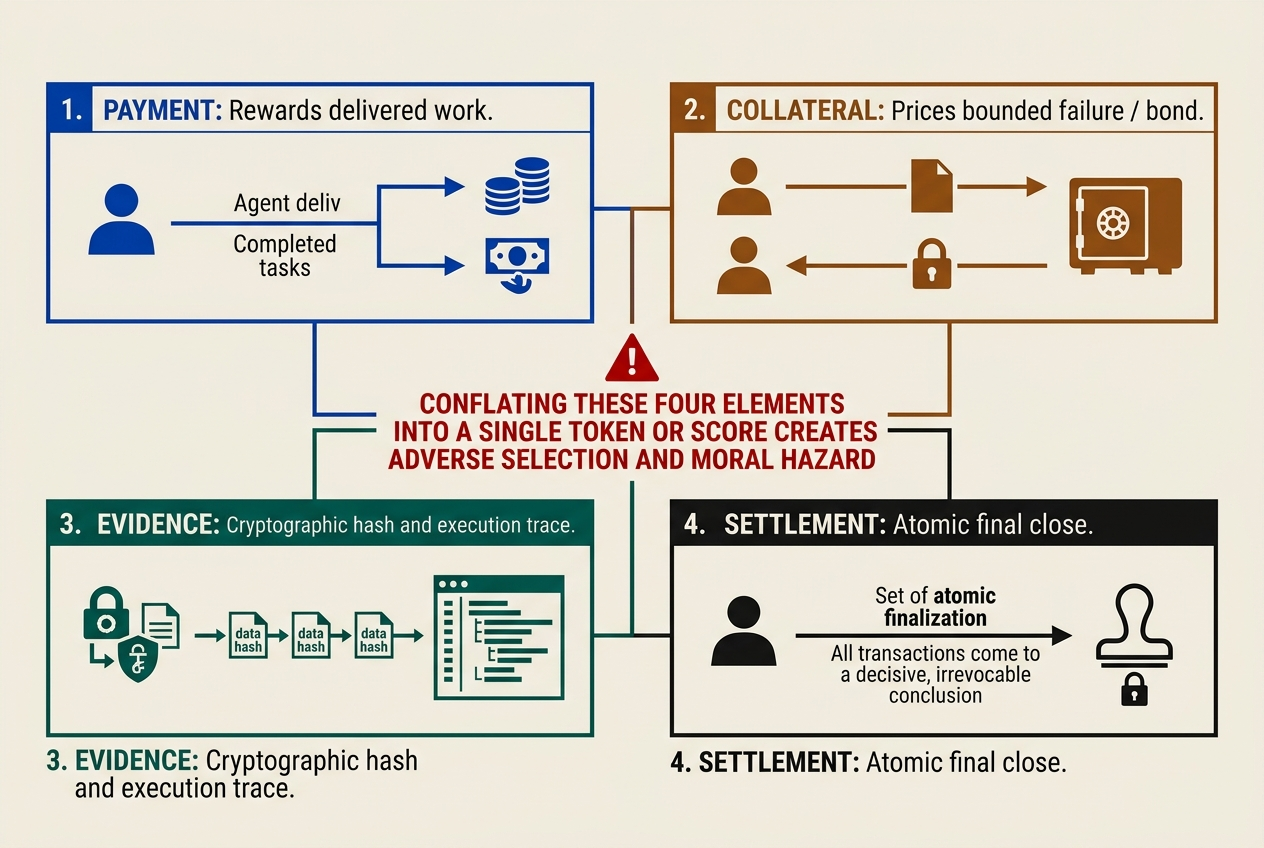
\includegraphics[width=\pdfullwidth]{figures/fig-spark-prop6-instruments.jpg}%
  }
  \pdwidecaption{\textbf{Proposition 6 Mechanics: Four Separated Market Instruments.} To eliminate moral hazard and adverse selection in multi-agent trading, the kernel strictly separates Payment (labor compensation), Collateral (failure bonding), Evidence (execution proofs), and Settlement (atomic obligation closure).}[fig:spark-prop6]
\end{figure}

Under this separated architecture, an agent offering a service must post collateral $C \ge \mathcal{V}(\text{risk})$ into escrow. When the task completes, the contractor produces evidence $\mathcal{E}$ (test logs, diff hashes). Only when $\mathcal{E}$ satisfies the verifier contract does settlement $\mathcal{S}$ execute, simultaneously disbursing payment $P$, returning collateral $C$, and updating the reputation ledger. Conflating payment and collateral into a single balance allows defaulting agents to consume resources without recourse; separating them enforces incentive compatibility.

\subsubsection*{Proposition 7: Uncertainty Needs an Institution (\pdchapref{bonded}{The Bonded Commons})}
In complex software engineering, deterministic formal verification cannot decide every semantic property, and static type checkers cannot foresee every runtime interaction. Managing residual uncertainty requires institutional governance, grounded in Ostrom's governing of shared commons~\pdcite{ostrom1990governing} and Becker's economics of deterrence~\pdcite{becker1968}.

Some harms cannot be prevented upfront, and some outcomes cannot be judged purely by mechanical test suites. To govern this irreducible uncertainty, the kernel constructs institutional procedures: bonded stake deposits, randomized spot audits by independent witness verifiers, neutral contestation and appeal arbitration, and strict conservation rules. By turning uncertainty into an inspectable, contested process backed by financial slashing, the commons deters defection while providing due process for false positives.

\begin{figure}[htbp]
  \pdpagecentered[\pdfullwidth]{%
    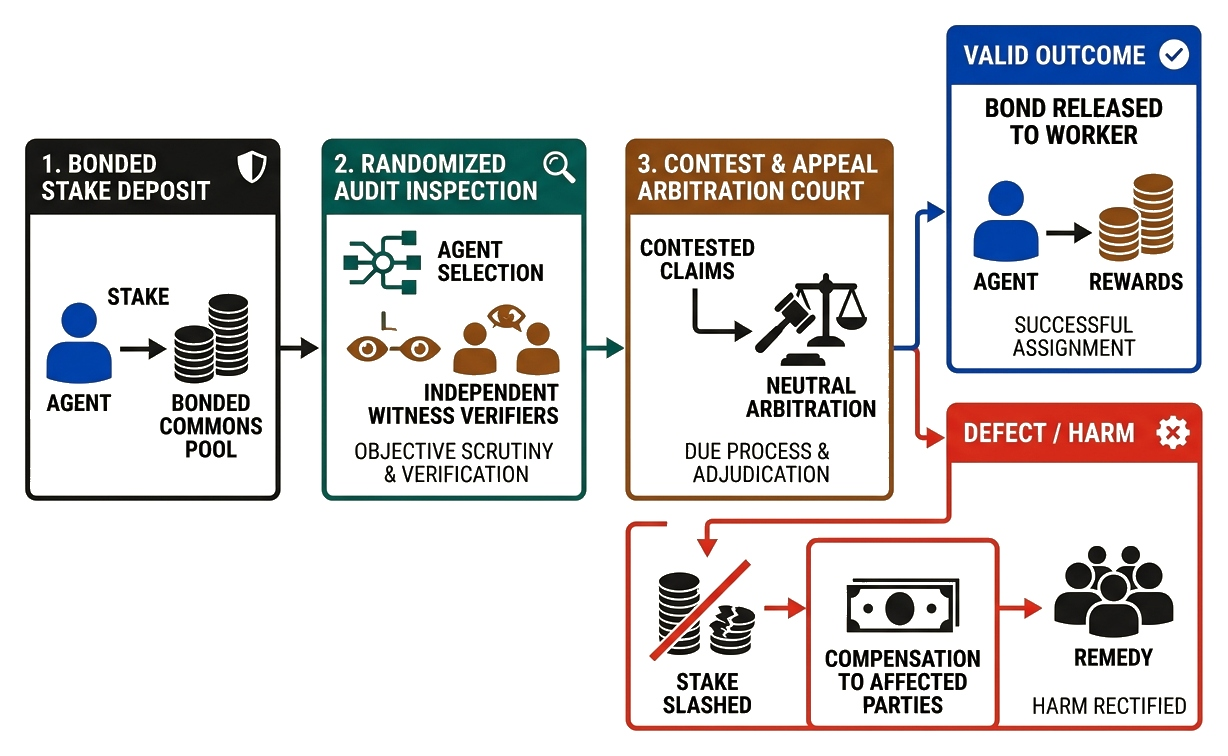
\includegraphics[width=\pdfullwidth]{figures/fig-spark-prop7-bonded.jpg}%
  }
  \pdwidecaption{\textbf{Proposition 7 Mechanics: Bonded Commons Governance.} Shared host resources are governed as Common-Pool Resources (CPRs). Agents post bonded stake, undergo randomized independent verification audits, and face automated slashing upon invariant breach, balancing deterrence with due process.}[fig:spark-prop7]
\end{figure}

Following Becker's economic model of deterrence~\pdcite{becker1968}, the expected utility of defection $\mathbb{E}[U_{\text{defect}}]$ must be strictly negative:
\begin{equation}
\mathbb{E}[U_{\text{defect}}] \;=\; (1 - p_{\text{audit}}) \cdot G \;-\; p_{\text{audit}} \cdot S \;<\; 0
\end{equation}
where $G$ is the gain from unauthorized shortcutting (e.g., skipping tests), $p_{\text{audit}}$ is the probability of a randomized spot audit by a witness agent, and $S$ is the financial stake slashed upon discovery. By tuning $p_{\text{audit}}$ and $S$ such that $S > \frac{1 - p_{\text{audit}}}{p_{\text{audit}}} G$, the kernel sustains cooperation as a subgame-perfect Nash equilibrium.

\subsubsection*{Proposition 8: Federation Relays Evidence, Not Sovereignty (\pdchapref{fh}{The Federated Harbor})}
When autonomous fleets scale across distinct physical workstations, cloud tenancies, and organizational boundaries, centralizing all state into a single global database is both physically and politically impossible. Distributed machines operating under separate organizational ownership cannot submit to a single sovereign master.

Cross-machine federation must therefore exchange cryptographically verifiable evidence rather than shared state. Mutually distrustful hosts communicate across untrusted zero-trust relays, exchanging signed capability attestations, revocation gossips, Merkle inclusion proofs, and settlement receipts without sharing a database. Transport carries non-repudiable evidence; the receiving host's local kernel retains complete sovereignty over whether to admit, execute, or reject the requested operation.

\begin{figure}[htbp]
  \pdpagecentered[\pdfullwidth]{%
    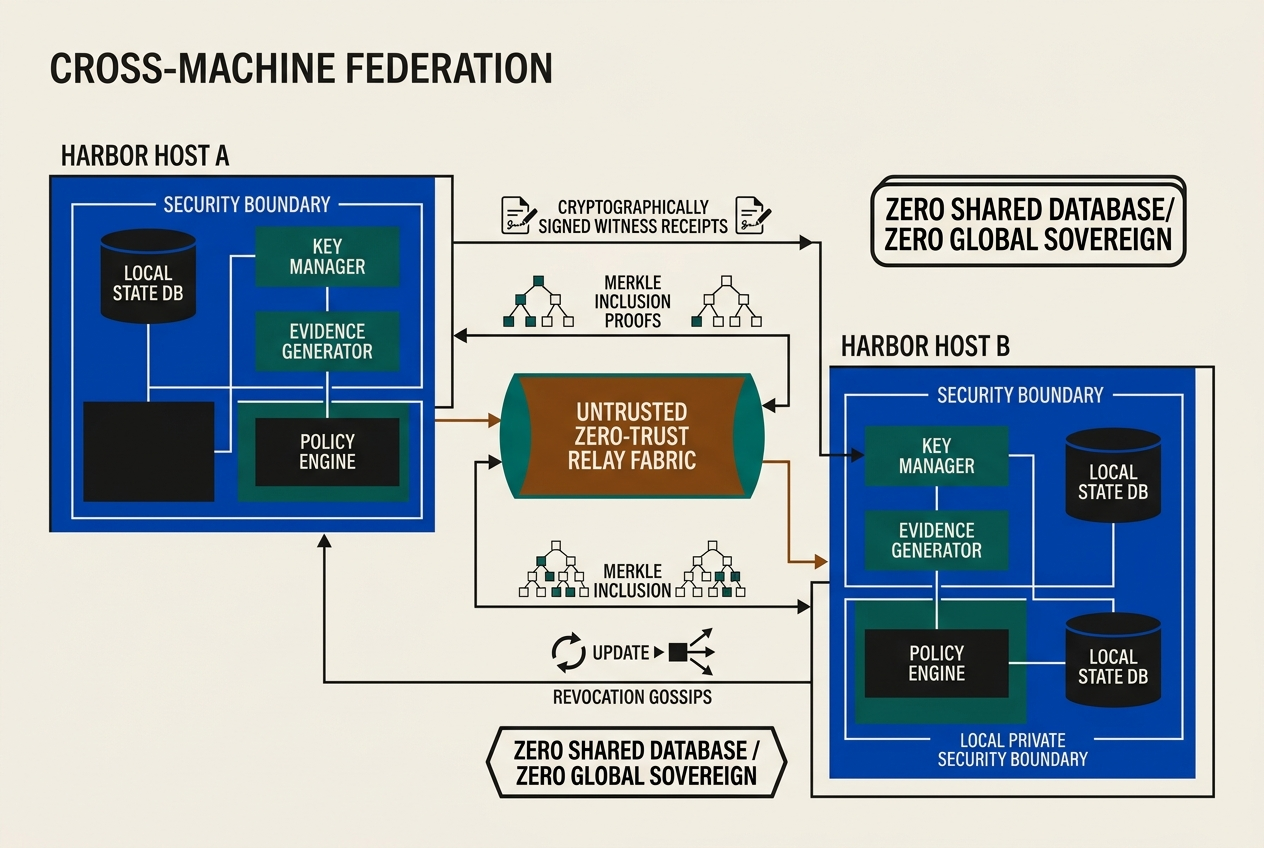
\includegraphics[width=\pdfullwidth]{figures/fig-spark-prop8-federation.jpg}%
  }
  \pdwidecaption{\textbf{Proposition 8 Mechanics: Federated Evidence Relay.} Cross-machine federation connects independent host kernels across zero-trust relays. Hosts exchange cryptographic proofs, witness receipts, and revocation gossips, retaining complete local sovereignty over resource admission without sharing a database.}[fig:spark-prop8]
\end{figure}

In this federated topology, host kernels $H_A, H_B$ maintain private, independent SQLite WAL databases. When Agent~$\alpha$ on host $H_A$ requests execution on host $H_B$, it transmits a signed credential package $\Pi = \langle \mathrm{sig}_A(\alpha), \mathrm{cap}_{\alpha}, \mathcal{M}_{\text{proof}} \rangle$. Host $H_B$'s local kernel independently verifies $\Pi$ against its local trust anchor, checking revocation state without querying $H_A$'s internal database. If valid, $H_B$ admits the task under local sandboxing rules. Sovereignty remains local; evidence crosses the wire.

Read these as a dependency chain: each chapter uses earlier mechanisms and
states what they cannot guarantee.

\subsection{What Counts as Knowing: Epistemic Bounds and Evidence Channels}
\pdmarginfigure{lovelace}{Ada Lovelace observed that analytical engines have no pretensions to originate anything; they execute what we know how to order them to perform.}%
Every consequential statement in this volume has a status and a boundary. Derivations establish
relations under named assumptions. Finite checks exhaust a stated state space,
not every deployment. Simulations estimate behavior under a stated generator;
repository tests exercise named paths; running code proves availability, not
universal mediation. Counterexamples remain in the record because they mark
claims the research killed rather than conclusions it merely failed to prove.

Evidence is typed as well. When a chapter reports what a harbor observed, it
names the channel that produced the observation, and each channel has a blind
spot that no amount of volume removes:
\begin{itemize}[leftmargin=1.8em,itemsep=2pt]
  \item A \emph{deterministic verifier} (a test, a type checker, a model checker) shows that a stated property holds of the artifact it examined, and nothing about properties it did not state.
  \item A \emph{provenance witness} (a signature, a hash, a Merkle inclusion, an append-only log) shows attribution and tamper-evidence relative to a commitment, never that every event was logged or that a description is true.
  \item A \emph{protected meter} (a counter its subject cannot rewrite) shows a quantity, not its cause.
  \item \emph{Expert judgment} shows an assessment under a named rubric and carries the assessor's error rate.
  \item \emph{Buyer preference} shows what was chosen, not that the choice was right.
  \item A \emph{delayed outcome} shows what happened, and arrives too late to prevent it.
\end{itemize}
The reader should ask the same question of any dashboard: which channel, and what can it not show.

\Cref{app:volume-status} gives the implementation boundary;
\cref{app:result-atlas} records the results and their limits. The companion
\path{docs/harbor-research/mega-volume-epistemic-manifest.yaml} preserves each
result's source, status, conditions, boundary, chapter home, and verification
artifact. The chapters stand alone; the book's claim is the chain they make.

\section{Classical Multi-Agent Systems Foundations}\label{sec:prereq-classical-mas}

Before analyzing neural coding agents, we formalize the foundational frameworks developed during the classical era of multi-agent systems.

\subsection{Intentional Agency and Practical Rationality}

Classical decision theory models an agent as an expected utility maximizer balancing subjective beliefs $\mathcal{B}$ and desires $\mathcal{D}$. In his seminal 1987 work \emph{Intention, Plans, and Practical Reason}, philosopher Michael Bratman demonstrated that this two-component model is computationally inadequate for resource-bounded agents operating in dynamic environments~\pdcite{bratman1987intention}.

A resource-bounded agent cannot continuously compute optimal policies from first principles at every millisecond. Practical rationality requires a third mental attitude: \textbf{Intention} ($\mathcal{I}$). Intentions are not merely desires with high utility; they represent \emph{conduct-controlling pro-attitudes to which the agent has actively committed}.

\pdmarginanalogy{prereq-flywheel-governor}{}{ch01-flywheel-governor}{Like a centrifugal flywheel governor throttling steam to stabilize rotational speed, practical rationality stabilizes an agent's intentions against transient sensor noise.}%
Bratman established four defining functional roles of intentions:
\begin{enumerate}[leftmargin=1.8em,itemsep=2pt]
  \item \textbf{Drive Means-End Reasoning:} An intention to achieve goal $\phi$ obligates the agent to formulate sub-plans and allocate computational cycles until $\phi$ is satisfied.
  \item \textbf{Filter of Admissibility:} Once an intention $\phi$ is adopted, candidate options inconsistent with $\phi$ (given current beliefs $\mathcal{B}$) are ruled inadmissible without evaluating their cost-benefit payoff.
  \item \textbf{Stability and Commitment:} Intentions resist reconsideration in the absence of relevant environmental interrupts or belief updates, preventing computational paralysis.
  \item \textbf{Coordination Scaffolding:} Intentions enable interpersonal coordination: other agents can safely form expectations regarding an agent's future actions based on its declared commitments.
\end{enumerate}

\subsection{The Rao--Georgeff BDI Temporal Logic (\texorpdfstring{$BDI_{CTL^*}$}{BDI-CTL*})}

Rao and Georgeff~\pdcite{rao1991modeling,rao1995bdi} formalized Bratman's theory into a multimodal branching-time temporal logic ($BDI_{CTL^*}$). A temporal world model $\mathcal{M}$ is defined as an 8-tuple:
\begin{equation}
\mathcal{M} \;=\; \langle W, T, \prec, U, \mathcal{B}, \mathcal{D}, \mathcal{I}, \Phi \rangle
\end{equation}
where $W$ is a set of possible worlds, $T$ is a discrete set of time points ordered by tree-branching relation $\prec$, $U$ is the universe of discourse, $\Phi$ interprets predicates across worlds and times, and $\mathcal{B}, \mathcal{D}, \mathcal{I} \subseteq W \times T \times W$ are accessibility relations for Beliefs, Desires, and Intentions.

For world $w \in W$ at time $t \in T$:
\begin{align}
\mathcal{B}_t(w) &= \{ w' \in W \mid (w, t, w') \in \mathcal{B} \} \\
\mathcal{D}_t(w) &= \{ w' \in W \mid (w, t, w') \in \mathcal{D} \} \\
\mathcal{I}_t(w) &= \{ w' \in W \mid (w, t, w') \in \mathcal{I} \}
\end{align}

Semantics of the mental modalities at state $\langle w, t \rangle$:
\begin{align}
\mathcal{M}, w, t \models \mathrm{Bel}(\phi) &\iff \forall w' \in \mathcal{B}_t(w), \; \mathcal{M}, w', t \models \phi \\
\mathcal{M}, w, t \models \mathrm{Des}(\phi) &\iff \forall w' \in \mathcal{D}_t(w), \; \mathcal{M}, w', t \models \phi \\
\mathcal{M}, w, t \models \mathrm{Int}(\phi) &\iff \forall w' \in \mathcal{I}_t(w), \; \mathcal{M}, w', t \models \phi
\end{align}

Beliefs satisfy the $KD45$ axiom system (deductive closure $\mathbf{K}$, consistency $\mathbf{D}$, positive introspection $\mathbf{4}$, and negative introspection $\mathbf{5}$). Desires and Intentions satisfy seriality ($\mathbf{D}$), ensuring an agent never desires or intends logical contradictions ($\neg\mathrm{Des}(\bot)$ and $\neg\mathrm{Int}(\bot)$).

\subsubsection{Compatibility and Weak Realism}
In rational agency, an agent's desires and intentions must be constrained by its beliefs. Under the \textbf{Weak Realism} axiom, an agent cannot intend what it believes to be impossible:
\begin{equation}
\forall w \in W, \; \mathcal{I}_t(w) \cap \mathcal{B}_t(w) \neq \emptyset
\end{equation}
Syntactically, for temporal achievement goals:
\begin{equation}
\mathrm{Int}(\mathbf{A}\lozenge \phi) \;\to\; \neg\mathrm{Bel}(\neg\mathbf{E}\lozenge \phi)
\end{equation}
where $\mathbf{A}\lozenge \phi$ denotes ``$\phi$ holds eventually on all future paths,'' and $\mathbf{E}\lozenge \phi$ denotes ``$\phi$ holds on at least one branch.''

\subsection{Formal Commitment Strategies}

A commitment strategy dictates the precise formal conditions under which an agent drops an intention $\phi$. Rao and Georgeff~\pdcite{rao1991modeling} formalized three canonical strategies:

\begin{table}[H]
\centering
\small
\begin{tabularx}{\textwidth}{lX}
\toprule
\textbf{Commitment Strategy} & \textbf{Formal Drop Axiom} \\
\midrule
\textbf{Blind (Fanatical)} & Maintains $\mathrm{Int}(\mathbf{A}\lozenge \phi)$ until $\mathrm{Bel}(\phi)$ holds. \\
& $\mathrm{Int}(\mathbf{A}\lozenge \phi) \land \neg\mathrm{Bel}(\phi) \to \mathbf{A}\big(\mathrm{Int}(\mathbf{A}\lozenge \phi) \;\mathcal{U}\; \mathrm{Bel}(\phi)\big)$. \\
& \emph{Pathology:} Induces infinite loops if $\phi$ becomes physically impossible. \\
\addlinespace[3pt]
\textbf{Single-Minded} & Drops $\phi$ if achieved \emph{or} believed impossible. \\
& $\mathrm{Int}(\mathbf{A}\lozenge \phi) \land \neg\mathrm{Bel}(\phi) \land \mathrm{Bel}(\mathbf{E}\lozenge \phi) \to \mathbf{A}\big(\mathrm{Int}(\mathbf{A}\lozenge \phi) \;\mathcal{U}\; (\mathrm{Bel}(\phi) \lor \neg\mathrm{Bel}(\mathbf{E}\lozenge \phi))\big)$. \\
& \emph{Standard:} Balances persistence with dynamic feasibility. \\
\addlinespace[3pt]
\textbf{Open-Minded} & Drops $\phi$ if achieved, impossible, \emph{or no longer desired}. \\
& $\mathrm{Int}(\mathbf{A}\lozenge \phi) \land \dots \land \mathrm{Des}(\mathbf{A}\lozenge \phi) \to \mathbf{A}\big(\mathrm{Int}(\mathbf{A}\lozenge \phi) \;\mathcal{U}\; (\mathrm{Bel}(\phi) \lor \neg\mathrm{Bel}(\mathbf{E}\lozenge \phi) \lor \neg\mathrm{Des}(\mathbf{A}\lozenge \phi))\big)$. \\
\bottomrule
\end{tabularx}
\caption{Canonical commitment strategies in BDI agent architectures.}
\label{tab:commitment-strategies}
\end{table}

\begin{pdclaim}{Design invariant}{Commitment Persistence}\label{inv:commitment-persistence}
An agent's intention $\iota \in \mathcal{I}$ must not be abandoned merely because a single step incurs a transient tool failure. Intention reconsideration is an explicit state transition triggered by invariant failure or objective discharge, not an accidental consequence of context window truncation.
\end{pdclaim}

\subsection{Operational Semantics of AgentSpeak(L) and Normative Extensions}

AgentSpeak(L)~\pdcite{bordini2007agentspeak} provides structural operational semantics (SOS) for executing BDI agents. An agent configuration is a tuple $C = \langle bs, ps, is, \mathcal{E}, A \rangle$, where $bs$ is the belief base, $ps$ is the plan library, $is$ is the set of active intention stacks, $\mathcal{E}$ is the event queue, and $A$ is the action history.

The operational execution cycle is governed by three deterministic or priority-driven selection functions:
\begin{enumerate}[leftmargin=1.8em,itemsep=2pt]
  \item $S_E(\mathcal{E}) = \langle te, i \rangle$: Selects an event from $\mathcal{E}$ (e.g., belief change $+b$, goal addition $+!g$).
  \item $S_O(\mathrm{App})$: Selects a plan $(p, \theta)$ from the applicable plans whose context is entailed by $bs\theta$.
  \item $S_I(is) = i$: Selects which intention stack advances its execution step in the current cycle.
\end{enumerate}

When an action $a$ in plan $p$ fails during host execution, AgentSpeak semantics do not silently abort the agent; instead, the failure transition posts a failure event $-!g$ to $\mathcal{E}$, popping the failed plan frame and invoking explicit recovery plans:
\begin{equation}
\frac{\epsilon = \langle te, i \rangle, \quad \mathrm{App}(\mathrm{Rel}(te, ps), bs) = \emptyset}{\langle bs, ps, is, \mathcal{E}, A \rangle \;\longrightarrow\; \langle bs, ps, is, \mathcal{E} \cup \{\langle -!g, \mathrm{pop}(i) \rangle\}, A \rangle}
\end{equation}

Figure~\ref{fig:bdi-execution-flow} synthesizes this operational choice architecture, illustrating how autonomous systems select between reactive rules, static classical planning, and dynamic BDI execution.

\begin{figure}[htbp]
  \pdpagecentered[\pdfullwidth]{%
    % fig-ch0-bdi-execution.tex
% BDI Execution Flow and Operational Choice Architecture
% 100% native vector Swiss TikZ layout adhering to Harbor Figure Standard (v2).
% Guaranteed collision-free panel architecture with bounded text containers.

% pd-robot-glyphs.tex
% Authentic vector robot glyphs and system iconography for Port Daddy architectural figures.
% Provides 100% vector replacements matching the AI-generated diagram prototypes.

\ifdefined\pdrobotglyphsloaded\else
\def\pdrobotglyphsloaded{1}

% -----------------------------------------------------------------------------
% 1. Standard Standing Agent Robot (Base Model)
% Args: shift (x,y), color, scale
% -----------------------------------------------------------------------------
\newcommand{\pdrobotbase}[3][1.0]{%
  \begin{scope}[shift={#2},scale=#1]
    % Head
    \draw[fill=#3!85, draw=#3!95!black, line width=0.6pt, rounded corners=2pt] (-0.28, 0.22) rectangle (0.28, 0.58);
    % Dual Antennae
    \draw[line width=0.65pt, draw=#3!95!black] (-0.12, 0.58) -- (-0.16, 0.72);
    \draw[line width=0.65pt, draw=#3!95!black] (0.12, 0.58) -- (0.16, 0.72);
    \fill[pdamber!90!orange] (-0.16, 0.72) circle (0.038);
    \fill[pdamber!90!orange] (0.16, 0.72) circle (0.038);
    % Screen / Visor
    \draw[fill=hhink!90, draw=none, rounded corners=1.2pt] (-0.22, 0.28) rectangle (0.22, 0.52);
    % Eyes
    \fill[pdteal!35!white] (-0.11, 0.40) circle (0.04);
    \fill[pdteal!35!white] (0.11, 0.40) circle (0.04);
    % Mouth bar
    \draw[pdteal!35!white, line width=0.4pt] (-0.07, 0.33) -- (0.07, 0.33);
    % Ear bolts
    \draw[fill=pdslate!60, draw=#3!95!black, line width=0.4pt] (-0.32, 0.35) rectangle (-0.28, 0.45);
    \draw[fill=pdslate!60, draw=#3!95!black, line width=0.4pt] (0.28, 0.35) rectangle (0.32, 0.45);
    % Neck
    \draw[fill=pdslate!70, draw=#3!95!black, line width=0.4pt] (-0.08, 0.16) rectangle (0.08, 0.22);
    % Body / Torso
    \draw[fill=#3!85, draw=#3!95!black, line width=0.6pt, rounded corners=2pt] (-0.32, -0.28) rectangle (0.32, 0.16);
    % Chest panel
    \draw[fill=pdpage, draw=#3!70!black, line width=0.35pt, rounded corners=1pt] (-0.22, -0.12) rectangle (0.22, 0.10);
    \fill[pdhealth] (-0.13, -0.01) circle (0.03);
    \fill[pdamber] (0.0, -0.01) circle (0.03);
    \fill[pderror] (0.13, -0.01) circle (0.03);
    % Arms
    \draw[fill=#3!75, draw=#3!95!black, line width=0.45pt, rounded corners=1.2pt] (-0.44, -0.20) rectangle (-0.32, 0.10);
    \draw[fill=#3!75, draw=#3!95!black, line width=0.45pt, rounded corners=1.2pt] (0.32, -0.20) rectangle (0.44, 0.10);
    % Legs & Feet
    \draw[fill=pdslate!80, draw=#3!95!black, line width=0.45pt] (-0.24, -0.46) rectangle (-0.09, -0.28);
    \draw[fill=pdslate!80, draw=#3!95!black, line width=0.45pt] (0.09, -0.46) rectangle (0.24, -0.28);
    \draw[fill=pdslate!90!black, draw=#3!95!black, line width=0.45pt, rounded corners=1pt] (-0.28, -0.52) rectangle (-0.05, -0.44);
    \draw[fill=pdslate!90!black, draw=#3!95!black, line width=0.45pt, rounded corners=1pt] (0.05, -0.52) rectangle (0.28, -0.44);
  \end{scope}
}

% -----------------------------------------------------------------------------
% 2. Robot Holding Voting / Lease Token Tablet
% -----------------------------------------------------------------------------
\newcommand{\pdrobottoken}[3][1.0]{%
  \begin{scope}[shift={#2},scale=#1]
    % Head
    \draw[fill=#3!85, draw=#3!95!black, line width=0.6pt, rounded corners=2pt] (-0.28, 0.22) rectangle (0.28, 0.58);
    % Antenna
    \draw[line width=0.65pt, draw=#3!95!black] (0, 0.58) -- (0, 0.73);
    \fill[pdamber!90!orange] (0, 0.73) circle (0.04);
    % Screen / Visor
    \draw[fill=hhink!90, draw=none, rounded corners=1.2pt] (-0.22, 0.28) rectangle (0.22, 0.52);
    \fill[pdteal!35!white] (-0.11, 0.40) circle (0.04);
    \fill[pdteal!35!white] (0.11, 0.40) circle (0.04);
    \draw[pdteal!35!white, line width=0.4pt] (-0.07, 0.33) -- (0.07, 0.33);
    % Neck
    \draw[fill=pdslate!70, draw=#3!95!black, line width=0.4pt] (-0.08, 0.16) rectangle (0.08, 0.22);
    % Body
    \draw[fill=#3!85, draw=#3!95!black, line width=0.6pt, rounded corners=2pt] (-0.32, -0.28) rectangle (0.32, 0.16);
    % Legs & Feet
    \draw[fill=pdslate!80, draw=#3!95!black, line width=0.45pt] (-0.24, -0.46) rectangle (-0.09, -0.28);
    \draw[fill=pdslate!80, draw=#3!95!black, line width=0.45pt] (0.09, -0.46) rectangle (0.24, -0.28);
    \draw[fill=pdslate!90!black, draw=#3!95!black, line width=0.45pt, rounded corners=1pt] (-0.28, -0.52) rectangle (-0.05, -0.44);
    \draw[fill=pdslate!90!black, draw=#3!95!black, line width=0.45pt, rounded corners=1pt] (0.05, -0.52) rectangle (0.28, -0.44);
    % Arms holding tablet
    \draw[fill=#3!75, draw=#3!95!black, line width=0.45pt] (-0.42, -0.08) -- (-0.22, 0.05) -- (-0.18, 0.0) -- (-0.35, -0.13) -- cycle;
    \draw[fill=#3!75, draw=#3!95!black, line width=0.45pt] (0.42, -0.08) -- (0.22, 0.05) -- (0.18, 0.0) -- (0.35, -0.13) -- cycle;
    % Tablet
    \draw[fill=pdpage, draw=pdcobalt, line width=0.55pt, rounded corners=1.2pt] (-0.24, -0.18) rectangle (0.24, 0.18);
    \node[font=\fontsize{3.8}{4.5}\selectfont\bfseries\color{pdcobalt}] at (0, 0.06) {VOTING};
    \node[font=\fontsize{3.5}{4.2}\selectfont\bfseries\color{hhink}] at (0, -0.06) {TOKEN};
  \end{scope}
}

% -----------------------------------------------------------------------------
% 3. Robot at Laptop / Deliberation
% -----------------------------------------------------------------------------
\newcommand{\pdrobotlaptop}[3][1.0]{%
  \begin{scope}[shift={#2},scale=#1]
    % Head (Tilted slightly forward)
    \draw[fill=#3!85, draw=#3!95!black, line width=0.6pt, rounded corners=2pt] (-0.26, 0.22) rectangle (0.26, 0.56);
    % Dual Antennae
    \draw[line width=0.65pt, draw=#3!95!black] (-0.10, 0.56) -- (-0.14, 0.70);
    \draw[line width=0.65pt, draw=#3!95!black] (0.10, 0.56) -- (0.14, 0.70);
    \fill[pdteal] (-0.14, 0.70) circle (0.038);
    \fill[pdteal] (0.14, 0.70) circle (0.038);
    % Visor
    \draw[fill=hhink!90, draw=none, rounded corners=1.2pt] (-0.20, 0.28) rectangle (0.20, 0.50);
    \fill[pdteal!40!white] (-0.10, 0.38) circle (0.038);
    \fill[pdteal!40!white] (0.10, 0.38) circle (0.038);
    % Body
    \draw[fill=#3!85, draw=#3!95!black, line width=0.6pt, rounded corners=2pt] (-0.30, -0.26) rectangle (0.30, 0.18);
    % Legs (Seated)
    \draw[fill=pdslate!80, draw=#3!95!black, line width=0.45pt] (-0.25, -0.38) rectangle (0.25, -0.26);
    % Desk surface
    \draw[line width=1.0pt, pdslate!80!black] (-0.6, -0.38) -- (0.7, -0.38);
    % Laptop Base
    \draw[fill=pdslate!40, draw=pdslate!90!black, line width=0.45pt] (-0.05, -0.38) -- (0.50, -0.38) -- (0.46, -0.33) -- (-0.02, -0.33) -- cycle;
    % Laptop Screen
    \draw[fill=pdcobalt!90!black, draw=pdslate!90!black, line width=0.5pt, rounded corners=1pt] (0.42, -0.33) -- (0.52, 0.05) -- (0.15, 0.05) -- (0.08, -0.33) -- cycle;
    % Glowing Screen Text
    \draw[pdteal!50!white, line width=0.4pt] (0.18, -0.03) -- (0.42, -0.03);
    \draw[pdteal!50!white, line width=0.4pt] (0.16, -0.12) -- (0.38, -0.12);
    \draw[pdteal!50!white, line width=0.4pt] (0.14, -0.21) -- (0.34, -0.21);
    % Arms on keyboard
    \draw[fill=#3!75, draw=#3!95!black, line width=0.45pt] (-0.22, 0.05) to[out=-20,in=160] (0.12, -0.30) -- (0.18, -0.33) -- (-0.18, -0.05) -- cycle;
  \end{scope}
}

% -----------------------------------------------------------------------------
% 4. Red-and-White Disablement Barrier
% -----------------------------------------------------------------------------
\newcommand{\pdbarrierline}[4]{% (x1, y1) to (x2, y2)
  \draw[line width=4.5pt, white] (#1,#2) -- (#3,#4);
  \draw[line width=4.5pt, pderror, dashed, dash pattern=on 6pt off 6pt] (#1,#2) -- (#3,#4);
  \draw[line width=0.6pt, pderror!80!black] (#1,#2) -- (#3,#4);
}

% -----------------------------------------------------------------------------
% 5. Vector Iconography Definitions
% -----------------------------------------------------------------------------
% Crossed Tools (Wrench + Screwdriver)
\newcommand{\pdicontools}[2][1.0]{%
  \begin{scope}[shift={#2},scale=#1]
    \draw[line width=1.4pt, pdslate!80!black, line cap=round] (-0.25,-0.25) -- (0.25,0.25);
    \draw[line width=1.4pt, pdrust!90!black, line cap=round] (-0.25,0.25) -- (0.25,-0.25);
    \draw[fill=pdslate!90!black, line width=0.4pt] (0.18,0.18) circle (0.10);
    \fill[white] (0.20,0.20) circle (0.04);
    \draw[fill=pdrust!90!black, line width=0.4pt] (0.20,-0.22) rectangle (0.26,-0.16);
  \end{scope}
}

% Git Branch
\newcommand{\pdicongit}[2][1.0]{%
  \begin{scope}[shift={#2},scale=#1]
    \draw[line width=1.1pt, pdteal!90!black] (0,-0.32) -- (0,0.32);
    \draw[line width=1.1pt, pdteal!90!black] (0,-0.08) to[out=45,in=180] (0.24,0.16);
    \fill[pdteal!90!black] (0,-0.24) circle (0.06);
    \fill[pdteal!90!black] (0,0.24) circle (0.06);
    \fill[pdteal!90!black] (0.24,0.16) circle (0.06);
  \end{scope}
}

% Network Globe
\newcommand{\pdiconglobe}[2][1.0]{%
  \begin{scope}[shift={#2},scale=#1]
    \draw[line width=0.7pt, pdcobalt!85!black] (0,0) circle (0.28);
    \draw[line width=0.5pt, pdcobalt!70] (0,0) ellipse (0.13 and 0.28);
    \draw[line width=0.5pt, pdcobalt!70] (-0.28,0) -- (0.28,0);
    \draw[line width=0.5pt, pdcobalt!70] (-0.24,0.14) -- (0.24,0.14);
    \draw[line width=0.5pt, pdcobalt!70] (-0.24,-0.14) -- (0.24,-0.14);
  \end{scope}
}

% Host OS Gear / Process
\newcommand{\pdicongear}[2][1.0]{%
  \begin{scope}[shift={#2},scale=#1]
    \fill[pdslate!75!black] (0,0) circle (0.22);
    \foreach \a in {0,45,90,135,180,225,270,315} {
      \fill[pdslate!75!black] (\a:0.26) circle (0.055);
    }
    \fill[white] (0,0) circle (0.09);
  \end{scope}
}

% Stopwatch / Timer
\newcommand{\pdicontimer}[2][1.0]{%
  \begin{scope}[shift={#2},scale=#1]
    \draw[line width=0.75pt, pdamber!90!black] (0,0) circle (0.25);
    \draw[line width=0.8pt, pdamber!90!black] (0,0.25) -- (0,0.33);
    \draw[line width=1.0pt, pdamber!90!black] (-0.06,0.33) -- (0.06,0.33);
    \draw[line width=0.75pt, pdamber!90!black] (0,0) -- (0,0.14);
    \draw[line width=0.75pt, pdamber!90!black] (0,0) -- (0.11,0.05);
    \fill[pdamber!90!black] (0,0) circle (0.035);
  \end{scope}
}

% Hardware Crash / Lightning Burst
\newcommand{\pdiconcrash}[2][1.0]{%
  \begin{scope}[shift={#2},scale=#1]
    \fill[pderror!90!black] (0.06,0.32) -- (-0.12,0.04) -- (-0.02,0.04) -- (-0.14,-0.32) -- (0.12,-0.02) -- (0.02,-0.02) -- cycle;
  \end{scope}
}

% Shield with Checkmark
\newcommand{\pdiconshieldcheck}[2][1.0]{%
  \begin{scope}[shift={#2},scale=#1]
    \fill[pdcobalt!90!black] (0,0.32) -- (0.26,0.20) to[out=-70,in=45] (0,-0.32) to[out=135,in=-110] (-0.26,0.20) -- cycle;
    \draw[line width=1.1pt, white, line cap=round, line join=round] (-0.11,-0.02) -- (-0.03,-0.12) -- (0.13,0.10);
  \end{scope}
}

% Padlock
\newcommand{\pdiconlock}[2][1.0]{%
  \begin{scope}[shift={#2},scale=#1]
    % Shackle
    \draw[line width=0.9pt, pdslate!80!black] (-0.12,0.05) -- (-0.12,0.18) arc (180:0:0.12) -- (0.12,0.05);
    % Body
    \draw[fill=pderror!85!black, draw=pderror!95!black, line width=0.5pt, rounded corners=1pt] (-0.18,-0.20) rectangle (0.18,0.06);
    % Keyhole
    \fill[white] (0,-0.04) circle (0.035);
    \draw[line width=0.6pt, white] (0,-0.04) -- (0,-0.13);
  \end{scope}
}

% Speedometer / Spend Cap
\newcommand{\pdiconspeedometer}[2][1.0]{%
  \begin{scope}[shift={#2},scale=#1]
    \draw[line width=1.0pt, pdteal!90!black] (-0.28,-0.04) arc (180:40:0.28);
    \draw[line width=1.0pt, pderror] (40:0.28) arc (40:0:0.28);
    \draw[line width=0.8pt, hhink, line cap=round] (0,-0.04) -- (0.12,0.14);
    \fill[hhink] (0,-0.04) circle (0.05);
  \end{scope}
}

% Sparkle Broom / Hygiene Wand
\newcommand{\pdiconbroom}[2][1.0]{%
  \begin{scope}[shift={#2},scale=#1]
    \draw[line width=1.2pt, pdteal!90!black, line cap=round] (-0.2,-0.2) -- (0.15,0.15);
    % Sparkles
    \fill[pdamber!90!orange] (0.22,0.22) circle (0.04);
    \fill[pdteal] (0.05,0.26) circle (0.03);
    \fill[pdteal] (0.26,0.05) circle (0.03);
  \end{scope}
}

% Host Terminal Substrate
\newcommand{\pdiconterminal}[2][1.0]{%
  \begin{scope}[shift={#2},scale=#1]
    \draw[fill=hhink!95, draw=pdslate!80, line width=0.6pt, rounded corners=1.5pt] (-0.35,-0.25) rectangle (0.35,0.25);
    \draw[fill=pderror] (-0.26,0.18) circle (0.025);
    \fill[pdamber] (-0.18,0.18) circle (0.025);
    \fill[pdhealth] (-0.10,0.18) circle (0.025);
    \node[font=\fontsize{4.5}{5}\selectfont\ttfamily\color{pdhealth}] at (0,-0.05) {>\_};
  \end{scope}
}

% Coins Stack
\newcommand{\pdiconcoins}[2][1.0]{%
  \begin{scope}[shift={#2},scale=#1]
    \foreach \y in {-0.24, -0.12, 0.0, 0.12} {
      \draw[fill=pdamber!80!orange, draw=pdamber!95!black, line width=0.45pt] (0,\y) ellipse (0.24 and 0.07);
    }
  \end{scope}
}

% Tall Coins Stack
\newcommand{\pdiconcoinstall}[2][1.0]{%
  \begin{scope}[shift={#2},scale=#1]
    \foreach \y in {-0.30, -0.18, -0.06, 0.06, 0.18, 0.30} {
      \draw[fill=pdamber!80!orange, draw=pdamber!95!black, line width=0.45pt] (0,\y) ellipse (0.24 and 0.07);
    }
  \end{scope}
}

% Slashed Coins (Stake Slashed)
\newcommand{\pdiconcoinslashed}[2][1.0]{%
  \begin{scope}[shift={#2},scale=#1]
    \foreach \y in {-0.20, -0.08, 0.04, 0.16} {
      \draw[fill=pdamber!70!white, draw=pdamber!80!black, line width=0.45pt] (0,\y) ellipse (0.22 and 0.065);
    }
    \draw[line width=1.5pt, pderror, line cap=round] (-0.26,-0.24) -- (0.26,0.24);
  \end{scope}
}

% Magnifying Glass (Audit Inspection)
\newcommand{\pdiconmagnifier}[2][1.0]{%
  \begin{scope}[shift={#2},scale=#1]
    \draw[line width=0.9pt, pdteal!90!black] (0,0.06) circle (0.16);
    \draw[line width=1.4pt, pdteal!90!black, line cap=round] (0.12,-0.06) -- (0.26,-0.20);
    \fill[white] (-0.04,0.10) circle (0.04);
  \end{scope}
}

% Arbitration Gavel & Scales of Justice
\newcommand{\pdiconarbitration}[2][1.0]{%
  \begin{scope}[shift={#2},scale=#1]
    % Central post
    \draw[line width=0.8pt, pdrust!90!black] (0.15,-0.20) -- (0.15,0.22);
    \draw[line width=0.8pt, pdrust!90!black] (-0.05,0.18) -- (0.35,0.18);
    \draw[line width=0.5pt, pdrust!80] (-0.05,0.18) -- (-0.12,0.02) -- (0.02,0.02) -- cycle;
    \draw[line width=0.5pt, pdrust!80] (0.35,0.18) -- (0.28,0.02) -- (0.42,0.02) -- cycle;
    % Gavel
    \draw[line width=1.4pt, pdrust!95!black, line cap=round] (-0.30,-0.18) -- (-0.10,0.05);
    \draw[fill=pdrust!90!black, draw=pdrust!95!black, line width=0.5pt, rounded corners=1pt] (-0.22,0.0) -- (-0.12,0.12) -- (-0.02,0.04) -- (-0.12,-0.08) -- cycle;
  \end{scope}
}

% Cash Bill / Liquidated Damages
\newcommand{\pdiconcash}[2][1.0]{%
  \begin{scope}[shift={#2},scale=#1]
    \draw[fill=white, draw=pdslate!90!black, line width=0.6pt, rounded corners=1.5pt] (-0.35,-0.20) rectangle (0.35,0.20);
    \draw[line width=0.5pt, pdteal!80!black] (-0.28,-0.14) rectangle (0.28,0.14);
    \fill[pdteal!90!black] (0,0) circle (0.08);
    \fill[pdteal!90!black] (-0.22,0) circle (0.035);
    \fill[pdteal!90!black] (0.22,0) circle (0.035);
  \end{scope}
}

% Group of People / Remedy
\newcommand{\pdicongrouppeople}[2][1.0]{%
  \begin{scope}[shift={#2},scale=#1]
    % Center person
    \fill[hhink] (0,0.12) circle (0.09);
    \fill[hhink] (-0.15,-0.20) to[out=70,in=180] (0,-0.02) to[out=0,in=110] (0.15,-0.20) -- cycle;
    % Left person
    \fill[hhgray!90!black] (-0.22,0.06) circle (0.075);
    \fill[hhgray!90!black] (-0.34,-0.20) to[out=70,in=180] (-0.22,-0.06) to[out=0,in=110] (-0.10,-0.20) -- cycle;
    % Right person
    \fill[hhgray!90!black] (0.22,0.06) circle (0.075);
    \fill[hhgray!90!black] (0.10,-0.20) to[out=70,in=180] (0.22,-0.06) to[out=0,in=110] (0.34,-0.20) -- cycle;
  \end{scope}
}

% Database Cylinder
\newcommand{\pdicondatabase}[2][1.0]{%
  \begin{scope}[shift={#2},scale=#1]
    \draw[fill=pdslate!20, draw=pdslate!90!black, line width=0.6pt] (-0.25,-0.15) rectangle (0.25,0.15);
    \draw[fill=pdslate!30, draw=pdslate!90!black, line width=0.5pt] (0,0.15) ellipse (0.25 and 0.08);
    \draw[draw=pdslate!90!black, line width=0.5pt] (-0.25,0) arc (180:360:0.25 and 0.08);
    \draw[draw=pdslate!90!black, line width=0.5pt] (-0.25,-0.15) arc (180:360:0.25 and 0.08);
  \end{scope}
}

% Signed Document / Witness Receipts
\newcommand{\pdicondocument}[2][1.0]{%
  \begin{scope}[shift={#2},scale=#1]
    \draw[fill=white, draw=pdslate!90!black, line width=0.55pt] (-0.18,-0.24) -- (0.10,-0.24) -- (0.18,-0.16) -- (0.18,0.24) -- (-0.18,0.24) -- cycle;
    \draw[draw=pdslate!80, line width=0.45pt] (0.10,-0.24) -- (0.10,-0.16) -- (0.18,-0.16);
    \draw[pdslate!70, line width=0.4pt] (-0.12,0.16) -- (0.12,0.16);
    \draw[pdslate!70, line width=0.4pt] (-0.12,0.08) -- (0.12,0.08);
    \draw[pdslate!70, line width=0.4pt] (-0.12,0.00) -- (0.06,0.00);
    % Feather / quill
    \draw[line width=0.7pt, pdcobalt!80!black] (0.08,-0.12) to[out=45,in=-45] (0.24,0.06);
  \end{scope}
}

% Merkle Inclusion Proof Tree
\newcommand{\pdiconmerkle}[2][1.0]{%
  \begin{scope}[shift={#2},scale=#1]
    % Root
    \draw[line width=0.5pt, pdslate!80] (0,0.20) -- (-0.16,0.04);
    \draw[line width=0.5pt, pdslate!80] (0,0.20) -- (0.16,0.04);
    \draw[line width=0.5pt, pdslate!80] (-0.16,0.04) -- (-0.24,-0.14);
    \draw[line width=0.5pt, pdslate!80] (-0.16,0.04) -- (-0.08,-0.14);
    \draw[line width=0.5pt, pdslate!80] (0.16,0.04) -- (0.08,-0.14);
    \draw[line width=0.5pt, pdslate!80] (0.16,0.04) -- (0.24,-0.14);
    \draw[fill=white, draw=pdslate!90!black, line width=0.4pt] (-0.05,0.16) rectangle (0.05,0.24);
    \draw[fill=white, draw=pdslate!90!black, line width=0.4pt] (-0.20,0.0) rectangle (-0.12,0.08);
    \draw[fill=white, draw=pdslate!90!black, line width=0.4pt] (0.12,0.0) rectangle (0.20,0.08);
    \draw[fill=pdteal!80!white, draw=pdteal!95!black, line width=0.5pt] (-0.28,-0.18) rectangle (-0.20,-0.10);
    \draw[fill=white, draw=pdslate!90!black, line width=0.4pt] (-0.12,-0.18) rectangle (-0.04,-0.10);
    \draw[fill=white, draw=pdslate!90!black, line width=0.4pt] (0.04,-0.18) rectangle (0.12,-0.10);
    \draw[fill=white, draw=pdslate!90!black, line width=0.4pt] (0.20,-0.18) rectangle (0.28,-0.10);
  \end{scope}
}

% Key (Cryptographic Key / Capability Key)
\newcommand{\pdiconkey}[2][1.0]{%
  \begin{scope}[shift={#2},scale=#1]
    \draw[line width=0.8pt, pdamber!95!black] (0, 0.12) circle (0.14);
    \fill[white] (0, 0.12) circle (0.06);
    \draw[line width=0.85pt, pdamber!95!black] (0, -0.02) -- (0, -0.26);
    \draw[line width=0.7pt, pdamber!95!black] (0, -0.14) -- (0.10, -0.14);
    \draw[line width=0.7pt, pdamber!95!black] (0, -0.22) -- (0.08, -0.22);
  \end{scope}
}

\def\pdiconclock{\pdicontimer}
\def\pdiconlightning{\pdiconcrash}

\fi

\pdfigurehue{pdcobalt}%
\begin{tikzpicture}[pd figure,x=1cm,y=1cm]
  \tikzset{
    containerbox/.style={
      draw=pdslate!40,
      line width=0.75pt,
      fill=white,
      rounded corners=3pt
    },
    innercard/.style={
      draw=pdslate!30,
      line width=0.55pt,
      fill=hhpaper!30,
      rounded corners=2pt,
      inner sep=3pt
    },
    flowarrow/.style={
      draw=pdcobalt,
      line width=0.8pt,
      ->,
      >=Stealth
    },
    feedbackarrow/.style={
      draw=pdteal!80!black,
      line width=0.8pt,
      ->,
      >=Stealth
    }
  }

  % =========================================================================
  % PANEL 1: PARADIGM SPECTRUM (Left: x in [0.1, 4.1], y in [0.4, 5.5])
  % =========================================================================
  \draw[containerbox] (0.1, 0.4) rectangle (4.1, 5.5);
  \fill[fill=pdslate!85!black, rounded corners=2pt] (0.14, 5.12) rectangle (4.06, 5.46);
  \node[anchor=center] at (2.1, 5.29) {%
    \fontsize{5.2}{6.2}\selectfont\bfseries\color{white}PARADIGM SPECTRUM%
  };

  % Card 1.1: Reactive Systems
  \begin{scope}[shift={(0.3, 3.8)}]
    \draw[innercard] (0, 0) rectangle (3.5, 1.15);
    \node[anchor=north west, font=\fontsize{4.8}{5.8}\selectfont\bfseries\color{hhink}] at (0.15, 1.05) {1. Reactive Systems};
    % diagram
    \fill[pdslate!40] (0.45, 0.62) circle (0.11cm);
    \draw[->, line width=0.6pt, pdslate!80] (0.65, 0.62) -- (1.25, 0.62);
    \fill[pdslate!80, rounded corners=1pt] (1.35, 0.51) rectangle (1.95, 0.73);
    \node[anchor=north west, font=\fontsize{3.8}{4.6}\selectfont\color{hhgray!90!black}, text width=3.2cm] at (0.15, 0.42) {%
      Stateless Condition $\rightarrow$ Action mapping. Fast reflex, blind to future consequences.%
    };
  \end{scope}

  % Card 1.2: Classical Planning
  \begin{scope}[shift={(0.3, 2.3)}]
    \draw[innercard] (0, 0) rectangle (3.5, 1.35);
    \node[anchor=north west, font=\fontsize{4.8}{5.8}\selectfont\bfseries\color{hhink}] at (0.15, 1.25) {2. Classical Planning};
    % graph (lowered to avoid title)
    \fill[pdteal!70] (0.45, 0.68) circle (0.07cm);
    \draw[line width=0.5pt, pdteal] (0.45, 0.68) -- (0.95, 0.81) circle (0.06cm);
    \draw[line width=0.5pt, pdteal] (0.45, 0.68) -- (0.95, 0.55) circle (0.06cm);
    \draw[line width=0.5pt, pdteal] (0.95, 0.81) -- (1.55, 0.81) circle (0.06cm);
    \node[anchor=north west, font=\fontsize{3.8}{4.6}\selectfont\color{hhgray!90!black}, text width=3.2cm] at (0.15, 0.46) {%
      Static state-space search (STRIPS/PDDL). Full precomputation; brittle when state diverges.%
    };
  \end{scope}

  % Card 1.3: BDI Architecture
  \begin{scope}[shift={(0.3, 0.55)}]
    \draw[draw=pdcobalt!80, line width=0.75pt, fill=pdcobalt!6, rounded corners=2pt] (0, 0) rectangle (3.5, 1.6);
    \node[anchor=north west, font=\fontsize{5.0}{6.0}\selectfont\bfseries\color{pdcobalt}] at (0.15, 1.48) {3. BDI Cybernetic Agent};
    % loop icon (lowered to avoid title)
    \draw[->, line width=0.65pt, pdcobalt] (0.5, 0.95) to[out=50, in=130] (1.5, 0.95);
    \draw[->, line width=0.65pt, pdcobalt] (1.5, 0.80) to[out=-130, in=-50] (0.5, 0.80);
    \node[anchor=north west, font=\fontsize{3.8}{4.6}\selectfont\color{hhink}, text width=3.2cm] at (0.15, 0.68) {%
      Dynamic commitment to intentions, practical reasoning ($S_E, S_O, S_I$), continuous perception, and built-in failure recovery.%
    };
  \end{scope}

  % =========================================================================
  % PANEL 2: THE CORE BDI CYBERNETIC LOOP (Center: x in [4.3, 10.3])
  % =========================================================================
  \draw[containerbox] (4.3, 0.4) rectangle (10.3, 5.5);
  \fill[fill=pdcobalt!90!black, rounded corners=2pt] (4.34, 5.12) rectangle (10.26, 5.46);
  \node[anchor=center] at (7.3, 5.29) {%
    \fontsize{5.2}{6.2}\selectfont\bfseries\color{white}THE CORE BDI CYBERNETIC LOOP%
  };

  % Row 1: Event Queue, Belief Base, Desire Base
  % Event Queue (Left)
  \begin{scope}[shift={(5.4, 4.45)}]
    \draw[draw=pdcobalt, fill=white, line width=0.6pt, rounded corners=2pt] (-0.85, -0.32) rectangle (0.85, 0.32);
    \node[font=\fontsize{4.6}{5.5}\selectfont\bfseries\color{pdcobalt}, align=center] at (0, 0) {Event Queue ($E$)\\{\fontsize{3.6}{4.4}\selectfont external / internal}};
  \end{scope}

  % Desire Base (Right)
  \begin{scope}[shift={(9.2, 4.45)}]
    \draw[draw=pdcobalt, fill=white, line width=0.6pt, rounded corners=2pt] (-0.85, -0.32) rectangle (0.85, 0.32);
    \node[font=\fontsize{4.6}{5.5}\selectfont\bfseries\color{pdcobalt}, align=center] at (0, 0) {Desire Base ($D$)\\{\fontsize{3.6}{4.4}\selectfont candidate goals}};
  \end{scope}

  % Belief Base (Center Left)
  \begin{scope}[shift={(5.4, 3.45)}]
    \draw[draw=pdcobalt, fill=white, line width=0.6pt, rounded corners=2pt] (-0.85, -0.35) rectangle (0.85, 0.35);
    \node[font=\fontsize{4.6}{5.5}\selectfont\bfseries\color{pdcobalt}, align=center] at (0, 0) {Belief Base ($B$)\\{\fontsize{3.6}{4.4}\selectfont world facts \& obs}};
  \end{scope}

  % Selection Functions Stack (Center Right)
  \begin{scope}[shift={(8.3, 3.45)}]
    \draw[draw=pdslate!40, fill=hhpaper!40, rounded corners=2pt] (-1.7, -0.55) rectangle (1.7, 0.55);
    % SE
    \draw[fill=pdcobalt!15, draw=pdcobalt, line width=0.45pt, rounded corners=1.5pt] (-1.55, 0.20) rectangle (1.55, 0.46);
    \node[font=\fontsize{4.0}{4.8}\selectfont\bfseries\color{pdcobalt}] at (0, 0.33) {$S_E$: Event Selection Function};
    % SO
    \draw[fill=pdteal!15, draw=pdteal, line width=0.45pt, rounded corners=1.5pt] (-1.55, -0.13) rectangle (1.55, 0.13);
    \node[font=\fontsize{4.0}{4.8}\selectfont\bfseries\color{pdteal!90!black}] at (0, 0) {$S_O$: Option / Plan Selection Function};
    % SI
    \draw[fill=pdindigo!15, draw=pdindigo, line width=0.45pt, rounded corners=1.5pt] (-1.55, -0.46) rectangle (1.55, -0.20);
    \node[font=\fontsize{4.0}{4.8}\selectfont\bfseries\color{pdindigo!90!black}] at (0, -0.33) {$S_I$: Intention Selection Function};
  \end{scope}

  % Connections from E, B, D into Selection Functions
  \draw[flowarrow] (5.4, 4.13) -- (5.4, 3.8);
  \draw[flowarrow] (6.25, 4.45) -- (6.6, 3.7);
  \draw[flowarrow] (6.25, 3.45) -- (6.6, 3.45);
  \draw[flowarrow] (8.5, 4.13) to[out=-90, in=60] (8.3, 4.0);

  % Intention Stack (active executing plans)
  \begin{scope}[shift={(7.3, 2.15)}]
    \draw[draw=pdcobalt!90!black, fill=pdcobalt!10, line width=0.75pt, rounded corners=2pt] (-2.2, -0.35) rectangle (2.2, 0.35);
    \node[font=\fontsize{4.6}{5.5}\selectfont\bfseries\color{pdcobalt}, align=center] at (0, 0.10) {Intention Stack ($I$)};
    \node[font=\fontsize{3.6}{4.4}\selectfont\color{hhink}, align=center] at (0, -0.14) {Active committed plans awaiting execution};
  \end{scope}

  \draw[flowarrow] (8.3, 2.9) -- (7.8, 2.5);

  % Downward Action Dispatch
  \draw[flowarrow, line width=0.9pt] (7.3, 1.8) -- (7.3, 1.25);
  \node[anchor=west, font=\fontsize{4.0}{4.8}\selectfont\bfseries\color{pdcobalt}] at (7.35, 1.55) {Execute Action $a \in \pi$};

  % Robot Worker + Environment Box
  \begin{scope}[shift={(5.9, 0.85)}]
    \pdrobotbase[0.55]{(0, 0)}{pdcobalt}
  \end{scope}

  \begin{scope}[shift={(7.8, 0.85)}]
    \draw[fill=pdslate!90!black, draw=none, rounded corners=2pt] (-1.1, -0.28) rectangle (1.1, 0.28);
    \node[font=\fontsize{4.8}{5.8}\selectfont\bfseries\color{white}] at (0, 0) {Host Environment};
  \end{scope}

  % Perception Feedback Loop: strictly within Center Panel, running up at x=4.6
  \draw[feedbackarrow] (6.7, 0.85) -- (5.9, 0.85);
  \draw[feedbackarrow] (5.3, 0.85) to[out=180, in=-90] (4.62, 1.8) -- (4.62, 3.1) to[out=90, in=180] (5.4, 3.45);
  \node[anchor=center, font=\fontsize{3.5}{4.2}\selectfont\bfseries\color{pdteal!90!black}, fill=white, inner sep=1pt, rotate=90] at (4.62, 2.45) {Perceptions ($P$)};

  % =========================================================================
  % PANEL 3: FAILURE RECOVERY & INVARIANT GATE (Right: x in [10.5, 14.5])
  % =========================================================================
  \draw[containerbox] (10.5, 0.4) rectangle (14.5, 5.5);
  \fill[fill=pdslate!85!black, rounded corners=2pt] (10.54, 5.12) rectangle (14.46, 5.46);
  \node[anchor=center] at (12.5, 5.29) {%
    \fontsize{5.2}{6.2}\selectfont\bfseries\color{white}FAILURE RECOVERY \& GATE%
  };

  % Top: Outcome Evaluator
  \begin{scope}[shift={(12.5, 4.5)}]
    \draw[draw=pdslate!60, fill=hhpaper!40, line width=0.6pt, rounded corners=2pt] (-1.5, -0.32) rectangle (1.5, 0.32);
    \node[font=\fontsize{4.6}{5.5}\selectfont\bfseries\color{hhink}] at (0, 0) {Action Result Evaluator};
  \end{scope}

  % Link from Center Panel Environment to Right Panel Evaluator via clean vertical channel
  \draw[flowarrow, dashed] (8.9, 0.85) -- (10.4, 0.85) -- (10.4, 4.5) -- (11.0, 4.5);

  % Branch 1: Action Failure (-!g)
  \begin{scope}[shift={(11.45, 3.3)}]
    \draw[fill=pderror, draw=none] (0, 0) circle (0.24cm);
    \node[font=\fontsize{5.2}{6.2}\selectfont\bfseries\color{white}] at (0, 0) {-!g};
    \node[anchor=north, font=\fontsize{4.0}{4.8}\selectfont\bfseries\color{pderror}, align=center] at (0, -0.28) {%
      Failure Event\\Trigger%
    };
  \end{scope}

  % Branch 2: Invariant Gate (Success)
  \begin{scope}[shift={(13.55, 3.3)}]
    \draw[draw=pdhealth!90!black, fill=pdhealth!10, line width=0.75pt, rounded corners=2pt] (-0.55, -0.32) rectangle (0.55, 0.32);
    \pdiconlock[0.55]{(0, 0)}
    \node[anchor=north, font=\fontsize{4.0}{4.8}\selectfont\bfseries\color{pdhealth!90!black}, align=center] at (0, -0.36) {%
      Invariant Gate\\Verification%
    };
  \end{scope}

  \draw[->, line width=0.75pt, pderror] (12.0, 4.18) to[out=-120, in=90] (11.45, 3.6);
  \draw[->, line width=0.75pt, pdhealth!90!black] (13.0, 4.18) to[out=-60, in=90] (13.55, 3.65);

  % Failure Healing Action
  \begin{scope}[shift={(11.45, 1.4)}]
    \draw[draw=pderror!60, fill=pderror!6, line width=0.5pt, rounded corners=2pt] (-0.85, -0.55) rectangle (0.85, 0.55);
    \node[font=\fontsize{3.8}{4.6}\selectfont\color{hhink}, align=center, text width=1.5cm] at (0, 0) {%
      Pop failed plan\\from stack $\rightarrow$\\invoke alternative\\contingency plan%
    };
  \end{scope}
  \draw[->, line width=0.65pt, pderror] (11.45, 2.3) -- (11.45, 1.95);

  % Success Durable Memory Commit
  \begin{scope}[shift={(13.55, 1.4)}]
    \draw[draw=pdhealth!60, fill=pdhealth!6, line width=0.5pt, rounded corners=2pt] (-0.85, -0.55) rectangle (0.85, 0.55);
    \node[font=\fontsize{3.8}{4.6}\selectfont\bfseries\color{pdhealth!90!black}, align=center, text width=1.5cm] at (0, 0) {%
      Execution receipt\\cryptographically\\signed \& committed\\to durable memory%
    };
  \end{scope}
  \draw[->, line width=0.65pt, pdhealth!90!black] (13.55, 2.3) -- (13.55, 1.95);

\end{tikzpicture}
%
  }
  \pdwidecaption{\textbf{BDI Execution Flow and Operational Choice Architecture.} Grounded in real-world software engineering workflows, adapted from AgentSpeak(L) semantics (Bordini et al., 2007). Contrasting reactive rule triggers, static STRIPS-style planners, and dynamic BDI agents. The three core selection functions ($S_E$ for events, $S_O$ for applicable plans, and $S_I$ for intention stacks) arbitrate runtime goal scheduling, with explicit plan failure handling via the $-!g$ recovery event.}[fig:bdi-execution-flow]
\end{figure}

\subsubsection{Normative Extensions: Deontic Constraints and Regret Minimization}

In institutional multi-agent systems, agents are constrained by external norms (deontic logic). A norm is defined as a 6-tuple $N = \langle \mathrm{id}, \mathrm{Type}, \phi_{\text{act}}, \phi_{\text{tgt}}, d, \mathrm{Sanction} \rangle$, where $\mathrm{Type} \in \{\mathcal{O}, \mathcal{F}, \mathcal{P}\}$ (Obligation, Prohibition, Permission), $\phi_{\text{act}}$ is the activation context, $\phi_{\text{tgt}}$ is the target state, $d$ is the deadline, and $\mathrm{Sanction}$ is the penalty for violation.

To reconcile institutional norms with internal intentions, agents maintain an \textbf{Abstract Norm Base} ($ANB$) and evaluate instantiated norms in the \textbf{Norm Instance Base} ($NIB$). When norm instances conflict with active goals ($\mathrm{Plans}(is \cup N) = \emptyset$), the agent resolves the normative conflict by partitioning candidate norms into \textbf{Maximal Non-Conflicting Subsets} (MNCS), selecting the subset that minimizes maximum penalty under a \textbf{minimax regret} criterion:
\begin{equation}
S^* \;=\; \arg\min_{S \in \Omega} \max_{n_v \in N \setminus S} \mathrm{Cost}(\mathrm{Sanction}(n_v))
\end{equation}
This ensures that any deliberate norm violation is recorded in an immutable ledger alongside its formal justification.

\subsubsection{Why BDI Matters for LLMs: Curing Intention Drift and Hallucinatory Abandonment}
\label{sec:why-bdi-matters}

Why should modern software engineers, operating cutting-edge transformer models, care about a symbolic multi-agent theory formulated in 1987? The answer lies in the acute operational pathologies of unanchored autoregressive inference.

Stateless large language models have no innate concept of commitment. Conditioned strictly on next-token likelihood, an unanchored model can formulate an elegant multi-step refactoring plan at step $t$, only to completely abandon it at step $t+1$ upon encountering a minor compiler warning or linter diagnostic. In empirical developer workflows, models frequently exhibit three fatal failure modes:
\begin{enumerate}[leftmargin=1.8em,itemsep=2pt]
  \item \textbf{Intention Drift:} As intermediate tool output scrolls across the prompt buffer, attention dilution causes the agent to lose focus on its primary objective, drifting into endless exploratory side-quests.
  \item \textbf{Spurious Abandonment:} Encountering an unexpected error code, an unanchored agent often prematurely declares a task ``impossible'' and hallucinations a false victory, or completely resets its approach, discarding hundreds of lines of valid working diffs.
  \item \textbf{Infinite Re-planning Loops:} Lacking explicit commitment axioms, models repeatedly re-generate the same high-level task plan rather than executing intermediate action steps.
\end{enumerate}

BDI practical rationality~\pdcite{bratman1987intention,rao1991modeling} provides the exact mathematical scaffold required to stabilize neural agents:
\begin{itemize}[leftmargin=1.8em,itemsep=2pt]
  \item \textbf{What We Adopt (Single-Minded Commitment):}\enspace In an Agent Operating Kernel, the user's high-level goal is converted into a durable intention $\iota \in \mathcal{I}$ registered in the kernel's state machine. The agent operates under \textbf{single-minded commitment}: it is forbidden from abandoning $\iota$ unless it produces proof that $\iota$ has been satisfied (e.g., passing test suite receipts) or an unrecoverable invariant failure proves $\neg\mathbf{E}\lozenge \iota$ (e.g., compile error in upstream vendor package).
  \item \textbf{What We Reject (Rigid Symbolic Plan Libraries):}\enspace Classical BDI required human programmers to hand-code every applicable plan $p \in ps$ in advance. We reject this rigidity. In our hybrid architecture, the neural language model acts as an open-ended, highly creative \emph{plan generator} and \emph{replanning engine}, while the deterministic BDI kernel enforces the \emph{intention stack}, monitors commitment persistence, and drives the $-!g$ failure recovery loop.
\end{itemize}

\subsection{Concurrency Foundations: Hewitt--Agha Actors vs. Hoare's Communicating Sequential Processes}

When multiple agents deliberate and execute concurrently on a developer's workstation, the concurrency substrate dictates whether the swarm operates harmoniously or degenerates into deadlocks and corrupted file state. Distributed systems research provides two foundational, mathematically rigorous concurrency paradigms:

\begin{itemize}[leftmargin=1.8em,itemsep=3pt]
  \item \textbf{Hewitt--Agha Actor Model (1973, 1986)~\pdcite{hewitt1973actor,agha1986actors}:}\enspace
  The Actor Model treats the \textbf{actor} as the universal primitive of concurrent computation. An actor is an autonomous, computational entity that encapsulates private state, a mailbox (message queue), and behavior. In response to a message, an actor can concurrently perform exactly three operations:
  \begin{enumerate}[leftmargin=1.5em,itemsep=1.5pt]
    \item \emph{Send} a finite number of messages to other actors with known addresses;
    \item \emph{Create} a finite number of new actors;
    \item \emph{Designate the replacement behavior} ($\mathtt{become}$) to be used for the next message it receives.
  \end{enumerate}
  Actors share \textbf{no mutable state}. Message passing is fundamentally \textbf{asynchronous}: sending is non-blocking, and messages are buffered in the recipient's mailbox.

  \item \textbf{Hoare's Communicating Sequential Processes (CSP) (1978)~\pdcite{hoare1978csp}:}\enspace
  CSP formalizes concurrent computation around \textbf{processes} communicating over synchronous, unbuffered \textbf{channels}. The core principles of CSP are:
  \begin{enumerate}[leftmargin=1.5em,itemsep=1.5pt]
    \item \emph{Synchronous Rendezvous:} Communication is an unbuffered handshake. The output event $c!v$ on channel $c$ and the input event $c?x$ must occur simultaneously ($\Delta t = 0$). Whichever process reaches the communication point first blocks until the other process arrives.
    \item \emph{Guarded Choice (Alternative):} A process can wait on multiple communication events simultaneously using the alternative construct ($\mathtt{alt}$), proceeding with whichever channel becomes ready first.
  \end{enumerate}
\end{itemize}

Figure~\ref{fig:actor-concurrency} details the dual concurrency architecture: Hewitt--Agha virtual actor isolation for stochastic deliberation, and Hoare's Communicating Sequential Processes (CSP) synchronous rendezvous for physical state mutations.

\begin{figure}[htbp]
  \pdpagecentered[\pdfullwidth]{%
    % fig-ch0-concurrency-actors-csp.tex
% Concurrency Foundations: Virtual Actors vs. CSP Rendezvous
% 100% native vector Swiss TikZ spatial replica of the AI-generated diagram prototype.

% pd-robot-glyphs.tex
% Authentic vector robot glyphs and system iconography for Port Daddy architectural figures.
% Provides 100% vector replacements matching the AI-generated diagram prototypes.

\ifdefined\pdrobotglyphsloaded\else
\def\pdrobotglyphsloaded{1}

% -----------------------------------------------------------------------------
% 1. Standard Standing Agent Robot (Base Model)
% Args: shift (x,y), color, scale
% -----------------------------------------------------------------------------
\newcommand{\pdrobotbase}[3][1.0]{%
  \begin{scope}[shift={#2},scale=#1]
    % Head
    \draw[fill=#3!85, draw=#3!95!black, line width=0.6pt, rounded corners=2pt] (-0.28, 0.22) rectangle (0.28, 0.58);
    % Dual Antennae
    \draw[line width=0.65pt, draw=#3!95!black] (-0.12, 0.58) -- (-0.16, 0.72);
    \draw[line width=0.65pt, draw=#3!95!black] (0.12, 0.58) -- (0.16, 0.72);
    \fill[pdamber!90!orange] (-0.16, 0.72) circle (0.038);
    \fill[pdamber!90!orange] (0.16, 0.72) circle (0.038);
    % Screen / Visor
    \draw[fill=hhink!90, draw=none, rounded corners=1.2pt] (-0.22, 0.28) rectangle (0.22, 0.52);
    % Eyes
    \fill[pdteal!35!white] (-0.11, 0.40) circle (0.04);
    \fill[pdteal!35!white] (0.11, 0.40) circle (0.04);
    % Mouth bar
    \draw[pdteal!35!white, line width=0.4pt] (-0.07, 0.33) -- (0.07, 0.33);
    % Ear bolts
    \draw[fill=pdslate!60, draw=#3!95!black, line width=0.4pt] (-0.32, 0.35) rectangle (-0.28, 0.45);
    \draw[fill=pdslate!60, draw=#3!95!black, line width=0.4pt] (0.28, 0.35) rectangle (0.32, 0.45);
    % Neck
    \draw[fill=pdslate!70, draw=#3!95!black, line width=0.4pt] (-0.08, 0.16) rectangle (0.08, 0.22);
    % Body / Torso
    \draw[fill=#3!85, draw=#3!95!black, line width=0.6pt, rounded corners=2pt] (-0.32, -0.28) rectangle (0.32, 0.16);
    % Chest panel
    \draw[fill=pdpage, draw=#3!70!black, line width=0.35pt, rounded corners=1pt] (-0.22, -0.12) rectangle (0.22, 0.10);
    \fill[pdhealth] (-0.13, -0.01) circle (0.03);
    \fill[pdamber] (0.0, -0.01) circle (0.03);
    \fill[pderror] (0.13, -0.01) circle (0.03);
    % Arms
    \draw[fill=#3!75, draw=#3!95!black, line width=0.45pt, rounded corners=1.2pt] (-0.44, -0.20) rectangle (-0.32, 0.10);
    \draw[fill=#3!75, draw=#3!95!black, line width=0.45pt, rounded corners=1.2pt] (0.32, -0.20) rectangle (0.44, 0.10);
    % Legs & Feet
    \draw[fill=pdslate!80, draw=#3!95!black, line width=0.45pt] (-0.24, -0.46) rectangle (-0.09, -0.28);
    \draw[fill=pdslate!80, draw=#3!95!black, line width=0.45pt] (0.09, -0.46) rectangle (0.24, -0.28);
    \draw[fill=pdslate!90!black, draw=#3!95!black, line width=0.45pt, rounded corners=1pt] (-0.28, -0.52) rectangle (-0.05, -0.44);
    \draw[fill=pdslate!90!black, draw=#3!95!black, line width=0.45pt, rounded corners=1pt] (0.05, -0.52) rectangle (0.28, -0.44);
  \end{scope}
}

% -----------------------------------------------------------------------------
% 2. Robot Holding Voting / Lease Token Tablet
% -----------------------------------------------------------------------------
\newcommand{\pdrobottoken}[3][1.0]{%
  \begin{scope}[shift={#2},scale=#1]
    % Head
    \draw[fill=#3!85, draw=#3!95!black, line width=0.6pt, rounded corners=2pt] (-0.28, 0.22) rectangle (0.28, 0.58);
    % Antenna
    \draw[line width=0.65pt, draw=#3!95!black] (0, 0.58) -- (0, 0.73);
    \fill[pdamber!90!orange] (0, 0.73) circle (0.04);
    % Screen / Visor
    \draw[fill=hhink!90, draw=none, rounded corners=1.2pt] (-0.22, 0.28) rectangle (0.22, 0.52);
    \fill[pdteal!35!white] (-0.11, 0.40) circle (0.04);
    \fill[pdteal!35!white] (0.11, 0.40) circle (0.04);
    \draw[pdteal!35!white, line width=0.4pt] (-0.07, 0.33) -- (0.07, 0.33);
    % Neck
    \draw[fill=pdslate!70, draw=#3!95!black, line width=0.4pt] (-0.08, 0.16) rectangle (0.08, 0.22);
    % Body
    \draw[fill=#3!85, draw=#3!95!black, line width=0.6pt, rounded corners=2pt] (-0.32, -0.28) rectangle (0.32, 0.16);
    % Legs & Feet
    \draw[fill=pdslate!80, draw=#3!95!black, line width=0.45pt] (-0.24, -0.46) rectangle (-0.09, -0.28);
    \draw[fill=pdslate!80, draw=#3!95!black, line width=0.45pt] (0.09, -0.46) rectangle (0.24, -0.28);
    \draw[fill=pdslate!90!black, draw=#3!95!black, line width=0.45pt, rounded corners=1pt] (-0.28, -0.52) rectangle (-0.05, -0.44);
    \draw[fill=pdslate!90!black, draw=#3!95!black, line width=0.45pt, rounded corners=1pt] (0.05, -0.52) rectangle (0.28, -0.44);
    % Arms holding tablet
    \draw[fill=#3!75, draw=#3!95!black, line width=0.45pt] (-0.42, -0.08) -- (-0.22, 0.05) -- (-0.18, 0.0) -- (-0.35, -0.13) -- cycle;
    \draw[fill=#3!75, draw=#3!95!black, line width=0.45pt] (0.42, -0.08) -- (0.22, 0.05) -- (0.18, 0.0) -- (0.35, -0.13) -- cycle;
    % Tablet
    \draw[fill=pdpage, draw=pdcobalt, line width=0.55pt, rounded corners=1.2pt] (-0.24, -0.18) rectangle (0.24, 0.18);
    \node[font=\fontsize{3.8}{4.5}\selectfont\bfseries\color{pdcobalt}] at (0, 0.06) {VOTING};
    \node[font=\fontsize{3.5}{4.2}\selectfont\bfseries\color{hhink}] at (0, -0.06) {TOKEN};
  \end{scope}
}

% -----------------------------------------------------------------------------
% 3. Robot at Laptop / Deliberation
% -----------------------------------------------------------------------------
\newcommand{\pdrobotlaptop}[3][1.0]{%
  \begin{scope}[shift={#2},scale=#1]
    % Head (Tilted slightly forward)
    \draw[fill=#3!85, draw=#3!95!black, line width=0.6pt, rounded corners=2pt] (-0.26, 0.22) rectangle (0.26, 0.56);
    % Dual Antennae
    \draw[line width=0.65pt, draw=#3!95!black] (-0.10, 0.56) -- (-0.14, 0.70);
    \draw[line width=0.65pt, draw=#3!95!black] (0.10, 0.56) -- (0.14, 0.70);
    \fill[pdteal] (-0.14, 0.70) circle (0.038);
    \fill[pdteal] (0.14, 0.70) circle (0.038);
    % Visor
    \draw[fill=hhink!90, draw=none, rounded corners=1.2pt] (-0.20, 0.28) rectangle (0.20, 0.50);
    \fill[pdteal!40!white] (-0.10, 0.38) circle (0.038);
    \fill[pdteal!40!white] (0.10, 0.38) circle (0.038);
    % Body
    \draw[fill=#3!85, draw=#3!95!black, line width=0.6pt, rounded corners=2pt] (-0.30, -0.26) rectangle (0.30, 0.18);
    % Legs (Seated)
    \draw[fill=pdslate!80, draw=#3!95!black, line width=0.45pt] (-0.25, -0.38) rectangle (0.25, -0.26);
    % Desk surface
    \draw[line width=1.0pt, pdslate!80!black] (-0.6, -0.38) -- (0.7, -0.38);
    % Laptop Base
    \draw[fill=pdslate!40, draw=pdslate!90!black, line width=0.45pt] (-0.05, -0.38) -- (0.50, -0.38) -- (0.46, -0.33) -- (-0.02, -0.33) -- cycle;
    % Laptop Screen
    \draw[fill=pdcobalt!90!black, draw=pdslate!90!black, line width=0.5pt, rounded corners=1pt] (0.42, -0.33) -- (0.52, 0.05) -- (0.15, 0.05) -- (0.08, -0.33) -- cycle;
    % Glowing Screen Text
    \draw[pdteal!50!white, line width=0.4pt] (0.18, -0.03) -- (0.42, -0.03);
    \draw[pdteal!50!white, line width=0.4pt] (0.16, -0.12) -- (0.38, -0.12);
    \draw[pdteal!50!white, line width=0.4pt] (0.14, -0.21) -- (0.34, -0.21);
    % Arms on keyboard
    \draw[fill=#3!75, draw=#3!95!black, line width=0.45pt] (-0.22, 0.05) to[out=-20,in=160] (0.12, -0.30) -- (0.18, -0.33) -- (-0.18, -0.05) -- cycle;
  \end{scope}
}

% -----------------------------------------------------------------------------
% 4. Red-and-White Disablement Barrier
% -----------------------------------------------------------------------------
\newcommand{\pdbarrierline}[4]{% (x1, y1) to (x2, y2)
  \draw[line width=4.5pt, white] (#1,#2) -- (#3,#4);
  \draw[line width=4.5pt, pderror, dashed, dash pattern=on 6pt off 6pt] (#1,#2) -- (#3,#4);
  \draw[line width=0.6pt, pderror!80!black] (#1,#2) -- (#3,#4);
}

% -----------------------------------------------------------------------------
% 5. Vector Iconography Definitions
% -----------------------------------------------------------------------------
% Crossed Tools (Wrench + Screwdriver)
\newcommand{\pdicontools}[2][1.0]{%
  \begin{scope}[shift={#2},scale=#1]
    \draw[line width=1.4pt, pdslate!80!black, line cap=round] (-0.25,-0.25) -- (0.25,0.25);
    \draw[line width=1.4pt, pdrust!90!black, line cap=round] (-0.25,0.25) -- (0.25,-0.25);
    \draw[fill=pdslate!90!black, line width=0.4pt] (0.18,0.18) circle (0.10);
    \fill[white] (0.20,0.20) circle (0.04);
    \draw[fill=pdrust!90!black, line width=0.4pt] (0.20,-0.22) rectangle (0.26,-0.16);
  \end{scope}
}

% Git Branch
\newcommand{\pdicongit}[2][1.0]{%
  \begin{scope}[shift={#2},scale=#1]
    \draw[line width=1.1pt, pdteal!90!black] (0,-0.32) -- (0,0.32);
    \draw[line width=1.1pt, pdteal!90!black] (0,-0.08) to[out=45,in=180] (0.24,0.16);
    \fill[pdteal!90!black] (0,-0.24) circle (0.06);
    \fill[pdteal!90!black] (0,0.24) circle (0.06);
    \fill[pdteal!90!black] (0.24,0.16) circle (0.06);
  \end{scope}
}

% Network Globe
\newcommand{\pdiconglobe}[2][1.0]{%
  \begin{scope}[shift={#2},scale=#1]
    \draw[line width=0.7pt, pdcobalt!85!black] (0,0) circle (0.28);
    \draw[line width=0.5pt, pdcobalt!70] (0,0) ellipse (0.13 and 0.28);
    \draw[line width=0.5pt, pdcobalt!70] (-0.28,0) -- (0.28,0);
    \draw[line width=0.5pt, pdcobalt!70] (-0.24,0.14) -- (0.24,0.14);
    \draw[line width=0.5pt, pdcobalt!70] (-0.24,-0.14) -- (0.24,-0.14);
  \end{scope}
}

% Host OS Gear / Process
\newcommand{\pdicongear}[2][1.0]{%
  \begin{scope}[shift={#2},scale=#1]
    \fill[pdslate!75!black] (0,0) circle (0.22);
    \foreach \a in {0,45,90,135,180,225,270,315} {
      \fill[pdslate!75!black] (\a:0.26) circle (0.055);
    }
    \fill[white] (0,0) circle (0.09);
  \end{scope}
}

% Stopwatch / Timer
\newcommand{\pdicontimer}[2][1.0]{%
  \begin{scope}[shift={#2},scale=#1]
    \draw[line width=0.75pt, pdamber!90!black] (0,0) circle (0.25);
    \draw[line width=0.8pt, pdamber!90!black] (0,0.25) -- (0,0.33);
    \draw[line width=1.0pt, pdamber!90!black] (-0.06,0.33) -- (0.06,0.33);
    \draw[line width=0.75pt, pdamber!90!black] (0,0) -- (0,0.14);
    \draw[line width=0.75pt, pdamber!90!black] (0,0) -- (0.11,0.05);
    \fill[pdamber!90!black] (0,0) circle (0.035);
  \end{scope}
}

% Hardware Crash / Lightning Burst
\newcommand{\pdiconcrash}[2][1.0]{%
  \begin{scope}[shift={#2},scale=#1]
    \fill[pderror!90!black] (0.06,0.32) -- (-0.12,0.04) -- (-0.02,0.04) -- (-0.14,-0.32) -- (0.12,-0.02) -- (0.02,-0.02) -- cycle;
  \end{scope}
}

% Shield with Checkmark
\newcommand{\pdiconshieldcheck}[2][1.0]{%
  \begin{scope}[shift={#2},scale=#1]
    \fill[pdcobalt!90!black] (0,0.32) -- (0.26,0.20) to[out=-70,in=45] (0,-0.32) to[out=135,in=-110] (-0.26,0.20) -- cycle;
    \draw[line width=1.1pt, white, line cap=round, line join=round] (-0.11,-0.02) -- (-0.03,-0.12) -- (0.13,0.10);
  \end{scope}
}

% Padlock
\newcommand{\pdiconlock}[2][1.0]{%
  \begin{scope}[shift={#2},scale=#1]
    % Shackle
    \draw[line width=0.9pt, pdslate!80!black] (-0.12,0.05) -- (-0.12,0.18) arc (180:0:0.12) -- (0.12,0.05);
    % Body
    \draw[fill=pderror!85!black, draw=pderror!95!black, line width=0.5pt, rounded corners=1pt] (-0.18,-0.20) rectangle (0.18,0.06);
    % Keyhole
    \fill[white] (0,-0.04) circle (0.035);
    \draw[line width=0.6pt, white] (0,-0.04) -- (0,-0.13);
  \end{scope}
}

% Speedometer / Spend Cap
\newcommand{\pdiconspeedometer}[2][1.0]{%
  \begin{scope}[shift={#2},scale=#1]
    \draw[line width=1.0pt, pdteal!90!black] (-0.28,-0.04) arc (180:40:0.28);
    \draw[line width=1.0pt, pderror] (40:0.28) arc (40:0:0.28);
    \draw[line width=0.8pt, hhink, line cap=round] (0,-0.04) -- (0.12,0.14);
    \fill[hhink] (0,-0.04) circle (0.05);
  \end{scope}
}

% Sparkle Broom / Hygiene Wand
\newcommand{\pdiconbroom}[2][1.0]{%
  \begin{scope}[shift={#2},scale=#1]
    \draw[line width=1.2pt, pdteal!90!black, line cap=round] (-0.2,-0.2) -- (0.15,0.15);
    % Sparkles
    \fill[pdamber!90!orange] (0.22,0.22) circle (0.04);
    \fill[pdteal] (0.05,0.26) circle (0.03);
    \fill[pdteal] (0.26,0.05) circle (0.03);
  \end{scope}
}

% Host Terminal Substrate
\newcommand{\pdiconterminal}[2][1.0]{%
  \begin{scope}[shift={#2},scale=#1]
    \draw[fill=hhink!95, draw=pdslate!80, line width=0.6pt, rounded corners=1.5pt] (-0.35,-0.25) rectangle (0.35,0.25);
    \draw[fill=pderror] (-0.26,0.18) circle (0.025);
    \fill[pdamber] (-0.18,0.18) circle (0.025);
    \fill[pdhealth] (-0.10,0.18) circle (0.025);
    \node[font=\fontsize{4.5}{5}\selectfont\ttfamily\color{pdhealth}] at (0,-0.05) {>\_};
  \end{scope}
}

% Coins Stack
\newcommand{\pdiconcoins}[2][1.0]{%
  \begin{scope}[shift={#2},scale=#1]
    \foreach \y in {-0.24, -0.12, 0.0, 0.12} {
      \draw[fill=pdamber!80!orange, draw=pdamber!95!black, line width=0.45pt] (0,\y) ellipse (0.24 and 0.07);
    }
  \end{scope}
}

% Tall Coins Stack
\newcommand{\pdiconcoinstall}[2][1.0]{%
  \begin{scope}[shift={#2},scale=#1]
    \foreach \y in {-0.30, -0.18, -0.06, 0.06, 0.18, 0.30} {
      \draw[fill=pdamber!80!orange, draw=pdamber!95!black, line width=0.45pt] (0,\y) ellipse (0.24 and 0.07);
    }
  \end{scope}
}

% Slashed Coins (Stake Slashed)
\newcommand{\pdiconcoinslashed}[2][1.0]{%
  \begin{scope}[shift={#2},scale=#1]
    \foreach \y in {-0.20, -0.08, 0.04, 0.16} {
      \draw[fill=pdamber!70!white, draw=pdamber!80!black, line width=0.45pt] (0,\y) ellipse (0.22 and 0.065);
    }
    \draw[line width=1.5pt, pderror, line cap=round] (-0.26,-0.24) -- (0.26,0.24);
  \end{scope}
}

% Magnifying Glass (Audit Inspection)
\newcommand{\pdiconmagnifier}[2][1.0]{%
  \begin{scope}[shift={#2},scale=#1]
    \draw[line width=0.9pt, pdteal!90!black] (0,0.06) circle (0.16);
    \draw[line width=1.4pt, pdteal!90!black, line cap=round] (0.12,-0.06) -- (0.26,-0.20);
    \fill[white] (-0.04,0.10) circle (0.04);
  \end{scope}
}

% Arbitration Gavel & Scales of Justice
\newcommand{\pdiconarbitration}[2][1.0]{%
  \begin{scope}[shift={#2},scale=#1]
    % Central post
    \draw[line width=0.8pt, pdrust!90!black] (0.15,-0.20) -- (0.15,0.22);
    \draw[line width=0.8pt, pdrust!90!black] (-0.05,0.18) -- (0.35,0.18);
    \draw[line width=0.5pt, pdrust!80] (-0.05,0.18) -- (-0.12,0.02) -- (0.02,0.02) -- cycle;
    \draw[line width=0.5pt, pdrust!80] (0.35,0.18) -- (0.28,0.02) -- (0.42,0.02) -- cycle;
    % Gavel
    \draw[line width=1.4pt, pdrust!95!black, line cap=round] (-0.30,-0.18) -- (-0.10,0.05);
    \draw[fill=pdrust!90!black, draw=pdrust!95!black, line width=0.5pt, rounded corners=1pt] (-0.22,0.0) -- (-0.12,0.12) -- (-0.02,0.04) -- (-0.12,-0.08) -- cycle;
  \end{scope}
}

% Cash Bill / Liquidated Damages
\newcommand{\pdiconcash}[2][1.0]{%
  \begin{scope}[shift={#2},scale=#1]
    \draw[fill=white, draw=pdslate!90!black, line width=0.6pt, rounded corners=1.5pt] (-0.35,-0.20) rectangle (0.35,0.20);
    \draw[line width=0.5pt, pdteal!80!black] (-0.28,-0.14) rectangle (0.28,0.14);
    \fill[pdteal!90!black] (0,0) circle (0.08);
    \fill[pdteal!90!black] (-0.22,0) circle (0.035);
    \fill[pdteal!90!black] (0.22,0) circle (0.035);
  \end{scope}
}

% Group of People / Remedy
\newcommand{\pdicongrouppeople}[2][1.0]{%
  \begin{scope}[shift={#2},scale=#1]
    % Center person
    \fill[hhink] (0,0.12) circle (0.09);
    \fill[hhink] (-0.15,-0.20) to[out=70,in=180] (0,-0.02) to[out=0,in=110] (0.15,-0.20) -- cycle;
    % Left person
    \fill[hhgray!90!black] (-0.22,0.06) circle (0.075);
    \fill[hhgray!90!black] (-0.34,-0.20) to[out=70,in=180] (-0.22,-0.06) to[out=0,in=110] (-0.10,-0.20) -- cycle;
    % Right person
    \fill[hhgray!90!black] (0.22,0.06) circle (0.075);
    \fill[hhgray!90!black] (0.10,-0.20) to[out=70,in=180] (0.22,-0.06) to[out=0,in=110] (0.34,-0.20) -- cycle;
  \end{scope}
}

% Database Cylinder
\newcommand{\pdicondatabase}[2][1.0]{%
  \begin{scope}[shift={#2},scale=#1]
    \draw[fill=pdslate!20, draw=pdslate!90!black, line width=0.6pt] (-0.25,-0.15) rectangle (0.25,0.15);
    \draw[fill=pdslate!30, draw=pdslate!90!black, line width=0.5pt] (0,0.15) ellipse (0.25 and 0.08);
    \draw[draw=pdslate!90!black, line width=0.5pt] (-0.25,0) arc (180:360:0.25 and 0.08);
    \draw[draw=pdslate!90!black, line width=0.5pt] (-0.25,-0.15) arc (180:360:0.25 and 0.08);
  \end{scope}
}

% Signed Document / Witness Receipts
\newcommand{\pdicondocument}[2][1.0]{%
  \begin{scope}[shift={#2},scale=#1]
    \draw[fill=white, draw=pdslate!90!black, line width=0.55pt] (-0.18,-0.24) -- (0.10,-0.24) -- (0.18,-0.16) -- (0.18,0.24) -- (-0.18,0.24) -- cycle;
    \draw[draw=pdslate!80, line width=0.45pt] (0.10,-0.24) -- (0.10,-0.16) -- (0.18,-0.16);
    \draw[pdslate!70, line width=0.4pt] (-0.12,0.16) -- (0.12,0.16);
    \draw[pdslate!70, line width=0.4pt] (-0.12,0.08) -- (0.12,0.08);
    \draw[pdslate!70, line width=0.4pt] (-0.12,0.00) -- (0.06,0.00);
    % Feather / quill
    \draw[line width=0.7pt, pdcobalt!80!black] (0.08,-0.12) to[out=45,in=-45] (0.24,0.06);
  \end{scope}
}

% Merkle Inclusion Proof Tree
\newcommand{\pdiconmerkle}[2][1.0]{%
  \begin{scope}[shift={#2},scale=#1]
    % Root
    \draw[line width=0.5pt, pdslate!80] (0,0.20) -- (-0.16,0.04);
    \draw[line width=0.5pt, pdslate!80] (0,0.20) -- (0.16,0.04);
    \draw[line width=0.5pt, pdslate!80] (-0.16,0.04) -- (-0.24,-0.14);
    \draw[line width=0.5pt, pdslate!80] (-0.16,0.04) -- (-0.08,-0.14);
    \draw[line width=0.5pt, pdslate!80] (0.16,0.04) -- (0.08,-0.14);
    \draw[line width=0.5pt, pdslate!80] (0.16,0.04) -- (0.24,-0.14);
    \draw[fill=white, draw=pdslate!90!black, line width=0.4pt] (-0.05,0.16) rectangle (0.05,0.24);
    \draw[fill=white, draw=pdslate!90!black, line width=0.4pt] (-0.20,0.0) rectangle (-0.12,0.08);
    \draw[fill=white, draw=pdslate!90!black, line width=0.4pt] (0.12,0.0) rectangle (0.20,0.08);
    \draw[fill=pdteal!80!white, draw=pdteal!95!black, line width=0.5pt] (-0.28,-0.18) rectangle (-0.20,-0.10);
    \draw[fill=white, draw=pdslate!90!black, line width=0.4pt] (-0.12,-0.18) rectangle (-0.04,-0.10);
    \draw[fill=white, draw=pdslate!90!black, line width=0.4pt] (0.04,-0.18) rectangle (0.12,-0.10);
    \draw[fill=white, draw=pdslate!90!black, line width=0.4pt] (0.20,-0.18) rectangle (0.28,-0.10);
  \end{scope}
}

% Key (Cryptographic Key / Capability Key)
\newcommand{\pdiconkey}[2][1.0]{%
  \begin{scope}[shift={#2},scale=#1]
    \draw[line width=0.8pt, pdamber!95!black] (0, 0.12) circle (0.14);
    \fill[white] (0, 0.12) circle (0.06);
    \draw[line width=0.85pt, pdamber!95!black] (0, -0.02) -- (0, -0.26);
    \draw[line width=0.7pt, pdamber!95!black] (0, -0.14) -- (0.10, -0.14);
    \draw[line width=0.7pt, pdamber!95!black] (0, -0.22) -- (0.08, -0.22);
  \end{scope}
}

\def\pdiconclock{\pdicontimer}
\def\pdiconlightning{\pdiconcrash}

\fi

\pdfigurehue{pdcobalt}%
\begin{tikzpicture}[pd figure,x=1cm,y=1cm]
  \tikzset{
    containerbox/.style={draw=pdslate!40,line width=0.7pt,fill=white,rounded corners=3.5pt},
    headerpill/.style={line width=0pt,rounded corners=2.5pt},
    usedforpill/.style={draw=none,fill=pdcobalt!90!black,rounded corners=2pt,inner xsep=6pt,inner ysep=2.5pt},
    cardbox/.style={draw=pdslate!30,line width=0.5pt,fill=hhpaper!30,rounded corners=2pt,inner sep=2pt}
  }

  % =========================================================================
  % LEFT PANEL: HEWITT-AGHA ACTOR MODEL (x in [0.1, 6.6])
  % =========================================================================
  \draw[containerbox] (0.1, 0.65) rectangle (6.6, 5.15);
  % Header (Navy)
  \draw[fill=pdcobalt!90!black,draw=none,rounded corners=2.5pt] (0.14, 4.75) rectangle (6.56, 5.11);
  \node[font=\fontsize{5.6}{6.8}\selectfont\bfseries\color{white}] at (3.35, 4.93) {%
    Hewitt-Agha Actor Model (Asynchronous)%
  };

  % Robot Receiver (Left)
  \pdrobotbase[0.65]{(0.9, 3.8)}{pdcobalt}
  \node[font=\fontsize{4.6}{5.4}\selectfont\color{hhink},align=center] at (2.2, 4.35) {%
    Receives messages\\{\fontsize{4.0}{4.8}\selectfont(capability tokens)}%
  };

  % Envelope with token
  \begin{scope}[shift={(1.85, 3.8)}]
    \draw[fill=white,draw=pdcobalt,line width=0.5pt,rounded corners=1pt] (-0.35, -0.22) rectangle (0.35, 0.22);
    \draw[line width=0.4pt,pdcobalt] (-0.35, 0.22) -- (0, -0.05) -- (0.35, 0.22);
    \draw[pd arrow,line width=0.6pt,pdcobalt] (0.45, 0) -- (0.85, 0);
  \end{scope}

  % Designated private mailbox
  \begin{scope}[shift={(2.5, 3.1)}]
    \draw[cardbox] (-1.0, -0.4) rectangle (1.0, 0.4);
    \node[font=\fontsize{4.6}{5.5}\selectfont\bfseries\color{hhink},align=center] at (0, 0.15) {%
      Designated\\private mailbox%
    };
    % mini queue bar
    \draw[fill=pdteal!30,draw=pdteal,line width=0.4pt,rounded corners=1pt] (-0.7, -0.3) rectangle (0.7, -0.08);
    \draw[pdteal,line width=0.4pt] (-0.25, -0.3) -- (-0.25, -0.08);
    \draw[pdteal,line width=0.4pt] (0.25, -0.3) -- (0.25, -0.08);
  \end{scope}

  % Isolated Private State (Right Column of Actor Panel)
  \begin{scope}[shift={(5.1, 3.3)}]
    \draw[draw=pdslate!40,line width=0.6pt,fill=hhpaper!15,rounded corners=2.5pt] (-1.25, -1.8) rectangle (1.25, 0.85);
    \node[font=\fontsize{4.8}{5.8}\selectfont\bfseries\color{pdcobalt}] at (0, 0.65) {Isolated Private State};
    % 3 Become pills
    \draw[fill=pdcobalt!85,draw=none,rounded corners=2pt] (-0.95, 0.15) rectangle (0.95, 0.48);
    \node[font=\fontsize{4.6}{5.5}\selectfont\bfseries\color{white}] at (0, 0.315) {become};

    \draw[fill=pdcobalt!85,draw=none,rounded corners=2pt] (-0.95, -0.35) rectangle (0.95, -0.02);
    \node[font=\fontsize{4.6}{5.5}\selectfont\bfseries\color{white}] at (0, -0.185) {become};

    \draw[fill=pdcobalt!85,draw=none,rounded corners=2pt] (-0.95, -0.85) rectangle (0.95, -0.52);
    \node[font=\fontsize{4.6}{5.5}\selectfont\bfseries\color{white}] at (0, -0.685) {become};

    \draw[pd arrow,line width=0.6pt,pdcobalt] (0, 0.15) -- (0, -0.02);
    \draw[pd arrow,line width=0.6pt,pdcobalt] (0, -0.35) -- (0, -0.52);
  \end{scope}

  % Asynchronous Queue label & arrow
  \node[font=\fontsize{4.6}{5.5}\selectfont\bfseries\color{hhink}] at (2.5, 2.35) {Asynchronous Queue};
  \draw[pd arrow,line width=0.8pt,pdcobalt] (1.3, 2.0) -- (3.7, 2.0);
  \node[font=\fontsize{4.2}{5.0}\selectfont\color{hhgray!90!black},align=center] at (1.5, 1.7) {Deposits\\message};
  \node[font=\fontsize{4.2}{5.0}\selectfont\color{hhgray!90!black},align=center] at (3.5, 1.7) {Process at\\own pace};

  % Bottom Pill: Used for
  \node[usedforpill,anchor=south] at (3.35, 0.72) {%
    {\fontsize{4.5}{5.4}\selectfont\color{white}\textbf{Used for:} Stochastic Agent Reasoning \& Isolated Sandboxes}%
  };

  % =========================================================================
  % RIGHT PANEL: HOARE CSP SYNCHRONOUS RENDEZVOUS (x in [6.9, 13.5])
  % =========================================================================
  \draw[containerbox] (6.9, 0.65) rectangle (13.5, 5.15);
  % Header (Teal)
  \draw[fill=pdteal!90!black,draw=none,rounded corners=2.5pt] (6.94, 4.75) rectangle (13.46, 5.11);
  \node[font=\fontsize{5.6}{6.8}\selectfont\bfseries\color{white}] at (10.2, 4.93) {%
    Hoare CSP Synchronous Rendezvous%
  };

  % Sender Robot (Left)
  \pdrobotbase[0.62]{(7.6, 3.8)}{pdteal}
  \node[font=\fontsize{4.6}{5.4}\selectfont\bfseries\color{hhink}] at (7.6, 4.45) {Sender};

  % Receiver Robot (Right)
  \pdrobotbase[0.62]{(12.8, 3.8)}{pdcobalt}
  \node[font=\fontsize{4.6}{5.4}\selectfont\bfseries\color{hhink}] at (12.8, 4.45) {Receiver};

  % Defined, unbuffered channel barrier (Interlocking Gate in Center)
  \begin{scope}[shift={(10.2, 3.8)}]
    \node[font=\fontsize{4.5}{5.4}\selectfont\bfseries\color{hhink},align=center] at (0, 0.65) {%
      Defined, unbuffered\\channel barrier%
    };
    % Interlocking Gate / Barrier
    \draw[fill=pdteal!30,draw=pdteal!90!black,line width=0.6pt] (-0.8, -0.3) rectangle (-0.2, 0.3);
    \draw[fill=pdcobalt!30,draw=pdcobalt!90!black,line width=0.6pt] (0.2, -0.3) rectangle (0.8, 0.3);
    \draw[fill=white,draw=pderror,line width=0.7pt,rounded corners=1pt] (-0.3, -0.15) rectangle (0.3, 0.15);
    \node[font=\fontsize{4.2}{5.0}\selectfont\bfseries\color{pderror}] at (0, 0) {Block};
  \end{scope}

  % Synchronous Handshake Card (Left Bottom of CSP)
  \begin{scope}[shift={(8.45, 2.25)}]
    \draw[cardbox] (-1.25, -0.7) rectangle (1.25, 0.55);
    \node[font=\fontsize{4.6}{5.5}\selectfont\bfseries\color{hhink}] at (0, 0.38) {Synchronous Handshake};
    % Status bar
    \draw[fill=pdhealth,draw=none] (-0.6, 0.12) rectangle (-0.3, 0.24);
    \draw[fill=pdhealth,draw=none] (-0.2, 0.12) rectangle (0.1, 0.24);
    \draw[fill=pdhealth,draw=none] (0.2, 0.12) rectangle (0.5, 0.24);
    \node[font=\fontsize{4.0}{4.8}\selectfont\bfseries\color{pdhealth!90!black}] at (0.8, 0.18) {Status};
    \node[font=\fontsize{4.2}{5.0}\selectfont\color{hhgray!90!black},align=center,text width=2.3cm] at (0, -0.28) {%
      Until at valive arrives\\to exchange data%
    };
  \end{scope}

  % Guarded External Choice Card (Right Bottom of CSP)
  \begin{scope}[shift={(11.95, 2.25)}]
    \draw[cardbox] (-1.25, -0.7) rectangle (1.25, 0.55);
    \node[font=\fontsize{4.6}{5.5}\selectfont\bfseries\color{hhink}] at (0, 0.38) {Guarded External Choice};
    % Bell / Alarm icon
    \pdiconcrash[0.45]{(-0.8, -0.05)}
    \node[font=\fontsize{4.2}{5.0}\selectfont\color{hhgray!90!black},align=left,text width=1.6cm] at (0.25, -0.1) {%
      Timeout alarm\\if choice isn't made\\prevent deadlocks%
    };
  \end{scope}

  % Bottom Pill: Used for
  \node[usedforpill,anchor=south] at (10.2, 0.72) {%
    {\fontsize{4.5}{5.4}\selectfont\color{white}\textbf{Used for:} Physical Host Resource Locks, Port Claims \& WAL Commits}%
  };

  % =========================================================================
  % BOTTOM FOOTER BANNER (x in [0.1, 13.5])
  % =========================================================================
  \node[draw=pdcobalt!40,line width=0.5pt,fill=pdcobalt!5,rounded corners=2pt,anchor=south,inner xsep=6pt,inner ysep=2.5pt] at (6.8, 0.1) {%
    {\fontsize{4.8}{5.8}\selectfont\color{hhink}\textbf{The Agent Kernel Synthesis:} Sovereign Actors communicate via Mailboxes; Scarce Physical Host Resources synchronize via CSP Barriers.}%
  };

\end{tikzpicture}
%
  }
  \pdwidecaption{\textbf{Concurrency Foundations for Multi-Agent Operating Kernels.} Synthesizing Hewitt--Agha virtual actor isolation (asynchronous mailboxes, capability tokens, and $\mathtt{become}$ state transitions) with Hoare's Communicating Sequential Processes (synchronous rendezvous barriers, $\Delta t = 0$, and guarded external choice with lease timeouts). Sovereign actors deliberate in isolated sandboxes, while physical host resource contention (TCP ports, SQLite WAL writes, git locks) is arbitrated via synchronous CSP rendezvous.}[fig:actor-concurrency]
\end{figure}

\subsection{From Asynchronous Isolation to Synchronous Rendezvous}

The fundamental divergence between Hewitt's Actor model and Hoare's Communicating Sequential Processes reflects an architectural trade-off between \emph{isolation} and \emph{synchronization}:

\begin{enumerate}[leftmargin=1.8em,itemsep=3pt]
  \item \textbf{Asynchronous Mailboxes vs.\ Unbuffered Barriers:}\enspace In the Actor model, communication is non-blocking and decoupled in time. An agent posts a message to a peer's mailbox and immediately resumes local execution. This temporal decoupling is indispensable for long-running neural inference loops: if an orchestrator were forced to block synchronously while a worker generated hundreds of tokens across a remote API, the entire supervisory loop would freeze. However, unbounded asynchronous mailboxes introduce severe hazards: message ordering is non-deterministic, queue backpressure is difficult to meter, and an agent can be flooded with stale context deltas.
  
  \item \textbf{Synchronous Rendezvous for Scarce Resources:}\enspace Conversely, Hoare's CSP enforces synchronous rendezvous: a send operation on an unbuffered channel cannot complete until a corresponding receive operation simultaneously executes. While synchronous rendezvous is prohibitive for stochastic agent inference, it is the mathematically optimal primitive for arbitrating scarce, physical, and non-fungible host resources: acquiring exclusive TCP port leases, linearizing commits in the SQLite write-ahead log (WAL), and locking git branch heads.
  
  \item \textbf{The Synthesis in an Agent Operating Kernel:}\enspace Modern agent operating kernels synthesize both lineages. As illustrated in Figure~\ref{fig:actor-concurrency}, workers execute as sovereign actors within seatbelted processes, receiving tasks through capability-attenuated mailboxes and recording state transitions via $\mathtt{become}$. Yet, whenever an actor attempts to alter shared reality, its request is arbitrated through Hoare-style synchronous barriers, guaranteeing mutual exclusion, preventing circular wait deadlocks through explicit lease timeouts, and ensuring deterministic linearizability.
\end{enumerate}

\subsubsection{Why Concurrency Lineages Matter: The Dual-Plane Operating Synthesis}
\label{sec:why-concurrency-matters}

Why should an autonomous agent infrastructure combine two historically competing concurrency models rather than adopting one exclusively? The answer is dictated by the physical constraints of developer machines and neural inference:
\begin{itemize}[leftmargin=1.8em,itemsep=2pt]
  \item \textbf{Why Pure CSP Fails for AI Agent Fleets:}\enspace If we built our multi-agent system purely on Hoare's Communicating Sequential Processes (as in Go channels or Occam), communication requires synchronous rendezvous ($\Delta t = 0$). Autoregressive token generation across frontier APIs is highly stochastic, with latencies ranging from 500 milliseconds to tens of seconds. Under pure CSP, an orchestrator process that sends a message to a worker is paralyzed until the worker consumes it. If two agents simultaneously attempt to query each other, or if a child process hangs on a remote API timeout, the entire swarm freezes in an irrecoverable circular rendezvous deadlock.
  \item \textbf{Why Pure Actors Fail on Local Workstations:}\enspace Conversely, if we built our system purely on Hewitt--Agha actors (as in Erlang/OTP or Akka), all communication is asynchronous and all state is private. But a developer workstation is not an abstract cluster: it possesses scarce, non-fungible, shared physical resources. There is only one TCP port 3000, one SQLite database file on disk, and one \texttt{.git/index} lock file. If five autonomous actors concurrently execute bash tool calls attempting to bind port 3000 or mutate the git repository without a synchronous arbitration barrier, the result is catastrophic: silent port squatting, broken working directories, and corrupted transaction logs.
  \item \textbf{What We Adopt in Port Daddy:}\enspace We implement a strict \textbf{Dual-Plane Architecture}. In the Deliberation Plane, agents are Hewitt--Agha actors: each subagent runs in an isolated OS process with private memory, communicating asynchronously over buffered mailbox queues and updating its internal state machine via $\mathtt{become}$. In the Physical Actuation Plane, all interactions with scarce host resources pass through Hoare CSP rendezvous barriers enforced by the supervisory daemon: atomic mutexes, lease timeouts, and single-writer commit gates that guarantee mutual exclusion and linearizability.
\end{itemize}

\subsection{Communicative Action and Speech Acts (FIPA-00037)}

Standard computer networks exchange raw byte packets; autonomous multi-agent engineering systems exchange \textbf{speech acts}. Grounded in Austin's distinction between locutionary (syntactic utterance), illocutionary (communicative intent), and perlocutionary (consequential effect) acts~\pdcite{austin1962how}, and Searle's taxonomy of illocutionary forces~\pdcite{searle1969speech}, the Foundation for Intelligent Physical Agents standardized the \textbf{FIPA ACL Communicative Act Library} (FIPA-00037)~\pdcite{fipa2002acl}.

In a developer's autonomous coding environment, speech acts are not abstract philosophy---they are the formal wire protocol between orchestrator agents, specialized coding subagents, and supervisory daemons. Every communicative act $a(s, r, \phi)$ between sender $s$ and receiver $r$ is formally defined by its \textbf{Feasibility Preconditions} ($FP$) and intended \textbf{Rational Effect} ($RE$). In an operating kernel, performatives cease to be informal chat tokens; they are cryptographically signed protocol events backed by content-addressed receipts. Consider a concrete developer scenario: an Orchestrator agent coordinates with a Database Supervisory agent to execute a non-blocking schema migration (\texttt{"add\_mfa\_col"}) while handling concurrent transaction load and generating synchronized TypeScript types. Table~\ref{tab:fipa-performatives} articulates these core performatives alongside their epistemic semantics:

\begin{table}[H]
\centering
\footnotesize
\setlength{\tabcolsep}{3pt}
\begin{tabularx}{\textwidth}{l l >{\raggedright\arraybackslash}X >{\raggedright\arraybackslash}X}
\toprule
\textbf{Act} & \textbf{Category} & \textbf{Feasibility Precondition ($FP$)} & \textbf{Rational Effect ($RE$)} \\
\midrule
\texttt{inform} & Assertive & $\mathrm{Bel}_s(\phi) \land \neg\mathrm{Bel}_s(\mathrm{Bel}_r(\phi))$ & $\mathrm{Bel}_r(\phi)$ \\
\texttt{request} & Directive & $\mathrm{FP}(\alpha)[s\backslash r] \land \mathrm{Bel}_s(\mathrm{Agent}(r, \alpha))$ & $\mathrm{Done}(\alpha)$ \\
\texttt{query-if} & Directive & $\neg\mathrm{Bel}_s(\phi) \land \neg\mathrm{Bel}_s(\neg\phi)$ & $\mathrm{Bel}_s(\mathrm{Bel}_r(\phi) \lor \mathrm{Bel}_r(\neg\phi))$ \\
\texttt{propose} & Commissive & $\mathrm{Bel}_s(\mathrm{Int}_s(\mathrm{Done}(\alpha, \phi)))$ & $\mathrm{Bel}_r(\mathrm{Int}_s(\mathrm{Done}(\alpha, \phi)))$ \\
\texttt{agree} & Commissive & $\mathrm{Bel}_s(\mathrm{Int}_s(\mathrm{Done}(\alpha)))$ & $\mathrm{Bel}_r(\mathrm{Int}_s(\mathrm{Done}(\alpha)))$ \\
\texttt{refuse} & Directive & $\mathrm{Bel}_s(\neg\mathrm{Int}_s(\mathrm{Done}(\alpha)))$ & $\mathrm{Bel}_r(\neg\mathrm{Int}_s(\mathrm{Done}(\alpha)))$ \\
\texttt{failure} & Assertive & $\mathrm{Bel}_s(\mathrm{Failed}(\alpha, \psi))$ & $\mathrm{Bel}_r(\mathrm{Failed}(\alpha, \psi))$ \\
\bottomrule
\end{tabularx}
\caption{FIPA-00037 communicative performatives with mental-state preconditions and rational effects.}
\label{tab:fipa-performatives}
\end{table}

\begin{figure}[htbp]
  \pdpagecentered[\pdfullwidth]{%
    % fig-ch0-fipa-speech-acts.tex
% FIPA-00037 Communicative Speech Act State Transition Machine
% Replaces raster fig-ch0-fipa-speech-acts.jpg with 100% native vector Swiss TikZ.
\pdfigurehue{pdindigo}%
\begin{tikzpicture}[pd figure,x=1cm,y=1cm]
  \tikzset{
    actnode/.style={draw=hhink,line width=0.7pt,fill=pdpage,rounded corners=2pt,align=center,font=\footnotesize,inner xsep=4pt,inner ysep=3pt},
    stateinit/.style={draw=pdindigo,line width=1.0pt,fill=pdindigo!8,rounded corners=3pt,align=center,font=\footnotesize,inner xsep=5pt,inner ysep=4pt},
    staterun/.style={draw=pdcobalt,line width=0.9pt,fill=pdcobalt!8,rounded corners=3pt,align=center,font=\footnotesize,inner xsep=5pt,inner ysep=4pt},
    statedone/.style={draw=pdhealth,line width=1.1pt,fill=pdhealth!10,rounded corners=3pt,align=center,font=\footnotesize,inner xsep=5pt,inner ysep=4pt},
    statefail/.style={draw=pderror,line width=0.9pt,dashed,fill=pderror!8,rounded corners=3pt,align=center,font=\footnotesize,inner xsep=5pt,inner ysep=4pt},
    panel/.style={draw=hhink!20,line width=0.5pt,densely dotted,rounded corners=3pt,fill=hhpaper!30}
  }

  % Three horizontal pipeline panels (height 3.2 each, 0.3 gap, total height 10.2)
  % =========================================================================
  % 1. DIRECTIVE PIPELINE: request (DB Migration under lock)
  % =========================================================================
  \draw[panel] (0.0,7.0) rectangle (15.2,10.2);
  \node[anchor=north west,font=\pdfiglabelsize\bfseries,text=pdindigo] at (0.2,9.95) {1. DIRECTIVE: \texttt{request} \normalfont\footnotesize\color{hhgray}(Atomic Action Execution)};
  \node[anchor=north east,font=\tiny\sffamily,text=hhgray] at (15.0,9.95) {$\langle\mathtt{conv\_id}, \mathtt{sender}, \mathtt{token}, \mathtt{action}\rangle$};

  % Row 1: Active Lifecycle (y = 8.8)
  \node[stateinit] (req_init) at (1.8,8.8) {%
    \textbf{Initiated}\\
    \scriptsize \texttt{request(db:migrate)}
  };

  \node[actnode,text width=2.6cm] (req_eval) at (5.4,8.8) {%
    \textbf{Arbitration}\\
    \scriptsize Lock \& capability
  };

  \node[staterun] (req_exec) at (9.6,8.8) {%
    \textbf{Agreed \& Sandboxed}\\
    \scriptsize \texttt{agree} $\to$ run migration
  };

  \node[statedone] (req_done) at (13.6,8.8) {%
    \textbf{Completed}\\
    \scriptsize \texttt{inform-done(receipt)}
  };

  % Row 2: Terminal Failure / Refusal (y = 7.55)
  \node[statefail,text width=2.8cm] (req_refuse) at (5.4,7.55) {%
    \textbf{Refused}\\
    \scriptsize \texttt{refuse(lock:held)}
  };

  \node[statefail,text width=2.8cm] (req_fail) at (9.6,7.55) {%
    \textbf{Failed}\\
    \scriptsize \texttt{failure(stderr)}
  };

  % Directive Arrows
  \draw[pd arrow,pdindigo] (req_init.east) -- (req_eval.west);
  \draw[pd arrow,pdcobalt] (req_eval.east) -- (req_exec.west);
  \draw[pd ready arrow] (req_exec.east) -- (req_done.west);
  \draw[pd breach arrow] (req_eval.south) -- (req_refuse.north);
  \draw[pd breach arrow] (req_exec.south) -- (req_fail.north);


  % =========================================================================
  % 2. ASSERTIVE PIPELINE: inform (Belief Base Mutation)
  % =========================================================================
  \draw[panel] (0.0,3.5) rectangle (15.2,6.7);
  \node[anchor=north west,font=\pdfiglabelsize\bfseries,text=pdteal] at (0.2,6.45) {2. ASSERTIVE: \texttt{inform} \normalfont\footnotesize\color{hhgray}(Belief Base Mutation)};
  \node[anchor=north east,font=\tiny\sffamily,text=hhgray] at (15.0,6.45) {Truth commitment: $\operatorname{Bel}_s(p) \land \operatorname{Des}_s(\operatorname{Bel}_r(p))$};

  % Row 1: Active Lifecycle (y = 5.3)
  \node[stateinit,draw=pdteal,fill=pdteal!8] (inf_init) at (1.8,5.3) {%
    \textbf{Asserted}\\
    \scriptsize \texttt{inform(status:green)}
  };

  \node[actnode,text width=2.6cm] (inf_verify) at (5.4,5.3) {%
    \textbf{Integrity Check}\\
    \scriptsize Ed25519 signature
  };

  \node[statedone] (inf_commit) at (13.6,5.3) {%
    \textbf{Belief Mutated}\\
    \scriptsize $+b \in bs$ committed to WAL
  };

  % Row 2: Malformed / Rejected (y = 4.05)
  \node[statefail,text width=3.4cm] (inf_rej) at (5.4,4.05) {%
    \textbf{Not Understood}\\
    \scriptsize \texttt{not-understood(bad:sig)}
  };

  % Assertive Arrows
  \draw[pd arrow,pdteal] (inf_init.east) -- (inf_verify.west);
  \draw[pd ready arrow] (inf_verify.east) -- node[above,font=\tiny,text=pdhealth] {valid cryptographic proof $\to$ commit} (inf_commit.west);
  \draw[pd breach arrow] (inf_verify.south) -- (inf_rej.north);


  % =========================================================================
  % 3. COMMISSIVE PIPELINE: propose (Contract / SLA Negotiation)
  % =========================================================================
  \draw[panel] (0.0,0.0) rectangle (15.2,3.2);
  \node[anchor=north west,font=\pdfiglabelsize\bfseries,text=pdgold] at (0.2,2.95) {3. COMMISSIVE: \texttt{propose} \normalfont\footnotesize\color{hhgray}(SLA \& Work Allocation)};
  \node[anchor=north east,font=\tiny\sffamily,text=hhgray] at (15.0,2.95) {Mutual covenant: $\operatorname{Int}_s(\alpha) \land \operatorname{Commit}(s, r, \alpha)$};

  % Row 1: Active Lifecycle (y = 1.8)
  \node[stateinit,draw=pdgold,fill=pdgold!10] (prop_init) at (1.8,1.8) {%
    \textbf{Proposed}\\
    \scriptsize \texttt{propose(sla:99.9\%)}
  };

  \node[actnode,text width=2.6cm] (prop_eval) at (5.4,1.8) {%
    \textbf{Utility Filter}\\
    \scriptsize Capacity \& budget
  };

  \node[staterun,draw=pdgold,fill=pdgold!8] (prop_acc) at (9.6,1.8) {%
    \textbf{Accepted}\\
    \scriptsize \texttt{accept-proposal}
  };

  \node[statedone] (prop_bound) at (13.6,1.8) {%
    \textbf{Escrow Bound}\\
    \scriptsize Bidirectional lease locked
  };

  % Row 2: Rejection (y = 0.55)
  \node[statefail,text width=2.8cm] (prop_rej) at (5.4,0.55) {%
    \textbf{Rejected}\\
    \scriptsize \texttt{reject-proposal}
  };

  % Commissive Arrows
  \draw[pd arrow,pdgold] (prop_init.east) -- (prop_eval.west);
  \draw[pd arrow,pdgold] (prop_eval.east) -- (prop_acc.west);
  \draw[pd ready arrow] (prop_acc.east) -- (prop_bound.west);
  \draw[pd breach arrow] (prop_eval.south) -- (prop_rej.north);

\end{tikzpicture}
%
  }
  \pdwidecaption{\textbf{FIPA-00037 Communicative Speech Act State Transition Machine.} Grounded in practical software engineering payloads. Top: Directive \texttt{request} lifecycle executing an atomic database migration under lock arbitration. Middle: Assertive \texttt{inform} directly mutating an agent's belief base. Bottom: Commissive \texttt{propose} negotiating an SLA for canary deployment routing. Every envelope carries cryptographic sender/receiver verification, monotonic capability tokens, and explicit conversation correlation IDs.}[fig:fipa-speech-acts]
\end{figure}

\subsubsection{Why Speech Acts Matter: From Conversational Fluff to Cryptographic Envelopes}
\label{sec:why-fipa-matters}

In naive multi-agent frameworks, agents communicate by exchanging raw natural language strings: ``\emph{Hey @database-agent, can you please run the migration and let me know when it's done?}'' This approach represents an acute engineering hazard:
\begin{enumerate}[leftmargin=1.8em,itemsep=2pt]
  \item \textbf{Syntactic and Pragmatic Ambiguity:} Natural language messages have fuzzy illocutionary force. Is the message an imperative command, a tentative proposal, or an informational suggestion? When an agent replies ``\emph{I'll look into it},'' has it committed to an intention or merely acknowledged receipt?
  \item \textbf{Conversational Fluff and Token Saturation:} Politeness tokens, preamble acknowledgments, and conversational pleasantries rapidly fill scarce prompt context windows, triggering premature compaction and attention dilution.
  \item \textbf{Vulnerability to Conversational Injection:} When communication consists of free-form text, an untrusted worker agent can craft adversarial dialogue prompts that manipulate the recipient's deliberation policy.
\end{enumerate}

The FIPA-00037 standard~\pdcite{fipa2002acl} provides the exact structural solution:
\begin{itemize}[leftmargin=1.8em,itemsep=2pt]
  \item \textbf{What We Adopt (Explicit Performative Envelopes):}\enspace We adopt FIPA's foundational illocutionary taxonomy: every message has a deterministic performative verb (\texttt{request}, \texttt{inform}, \texttt{propose}, \texttt{agree}, \texttt{refuse}, \texttt{failure}). In Port Daddy's Swarm Radio and Tube messaging fabrics, messages are never raw strings; they are structured binary or JSON envelopes containing the sender's cryptographic public key, recipient identifier, conversation correlation ID, performative type, and a typed payload conforming to a strict schema. An agent receiving a \texttt{request} knows with mathematical certainty that it is being asked to execute an action; an agent receiving an \texttt{agree} knows that a binding commitment has been formed.
  \item \textbf{What We Reject (Heavyweight Semantic Languages and Ontologies):}\enspace Classical FIPA required complex modal-logic semantic languages (FIPA SL) and heavyweight shared ontologies that required theorem provers to decode. We reject this runtime overhead. In our kernel, message bodies are strongly typed using Protocol Buffers or JSON Schemas, validated at wire-speed by the daemon before delivery, and cryptographically witnessed via Ed25519 signatures.
\end{itemize}

\subsection{Task Allocation: Smith's Contract Net Protocol (1980)}

Reid G. Smith's (1980) \textbf{Contract Net Protocol (CNP)}~\pdcite{smith1980cnp} formalized bilateral market-inspired negotiation between a Manager and distributed Contractor agents. In autonomous software fleets, CNP is the canonical mechanism for allocating urgent developer tasks---such as triage of a security CVE or compilation of an isolated package---across competing agent workers:

\begin{enumerate}[leftmargin=1.8em,itemsep=2pt]
  \item \textbf{Call for Proposals (CFP Broadcast):}\enspace The Manager broadcasts an announcement $\langle\mathtt{task\_id}, \allowbreak \mathtt{eligibility}, \allowbreak \mathtt{spec}, \allowbreak t_{\text{expire}}\rangle$ specifying required toolsets, maximum spend budget, and deadline.
  \item \textbf{Bidding and Capability Self-Assessment:}\enspace Eligible contractor agents inspect their current local capacity, sandboxed tools, and model context before submitting formal bids $\langle\mathtt{bid\_id}, \allowbreak \mathtt{cost}, \allowbreak \mathtt{eta}, \allowbreak \mathtt{reputation}\rangle$, or returning explicit refusals if overloaded.
  \item \textbf{Bid Evaluation and Award:}\enspace The Manager evaluates bids according to a multi-attribute utility function $\mathcal{U}_M(b) = w_r \cdot \text{rep} - w_c \cdot \text{cost} - w_t \cdot \text{eta}$, awarding an exclusive worktree lease to the winning contractor and rejecting alternative bids.
  \item \textbf{Execution, Interim Streaming, and Settlement:}\enspace The contractor checks out an isolated worktree branch, streams structured progress deltas, commits the diff, runs verification tests, and submits cryptographic execution receipts to unlock escrow payment.
\end{enumerate}

\begin{figure}[htbp]
  \pdpagecentered[\pdfullwidth]{%
    % fig-ch0-cnp-protocol.tex
% Contract Net Protocol (CNP) Market Allocation Lifecycle and Settlement
% Replaces raster fig-ch0-cnp-diagram.jpg with 100% native vector Swiss TikZ.
\pdfigurehue{pdcobalt}%
\begin{tikzpicture}[pd figure,x=1cm,y=1cm]
  \tikzset{
    actnode/.style={draw=hhink,line width=0.7pt,fill=pdpage,rounded corners=2pt,align=center,font=\footnotesize,inner xsep=4pt,inner ysep=3pt},
    stateinit/.style={draw=pdcobalt,line width=1.0pt,fill=pdcobalt!8,rounded corners=3pt,align=center,font=\footnotesize,inner xsep=5pt,inner ysep=4pt},
    staterun/.style={draw=pdteal,line width=0.9pt,fill=pdteal!8,rounded corners=3pt,align=center,font=\footnotesize,inner xsep=5pt,inner ysep=4pt},
    statedone/.style={draw=pdhealth,line width=1.1pt,fill=pdhealth!10,rounded corners=3pt,align=center,font=\footnotesize,inner xsep=5pt,inner ysep=4pt},
    statefail/.style={draw=pderror,line width=0.9pt,dashed,fill=pderror!8,rounded corners=3pt,align=center,font=\footnotesize,inner xsep=5pt,inner ysep=4pt},
    panel/.style={draw=hhink!20,line width=0.5pt,densely dotted,rounded corners=3pt,fill=hhpaper!30}
  }

  % =========================================================================
  % PHASE 1: MARKET CLEARING & BIDDING (LEFT PANEL)
  % =========================================================================
  \draw[panel] (0.0,0.0) rectangle (7.3,9.2);
  \node[anchor=north west,font=\pdfiglabelsize\bfseries,text=pdcobalt] at (0.2,8.95) {Phase 1: Bidding \& Award};
  \node[anchor=north east,font=\tiny\sffamily,text=hhgray] at (7.1,8.95) {Smith (1980)};

  % Manager Agent
  \node[actnode,draw=pdcobalt,fill=pdcobalt!8,text width=6.2cm] (mgr) at (3.65,7.8) {%
    \textbf{Manager Agent}\\[1pt]
    \scriptsize Task: \texttt{cve:patch} $\cdot$ Budget: \$0.00 $\cdot$ Deadline: $t_{\text{exp}}$
  };

  % CFP Broadcast
  \node[font=\tiny\ttfamily,text=pdcobalt,fill=hhpaper,draw=pdcobalt!40,rounded corners=2pt,inner sep=2pt] (cfp) at (3.65,6.7) {%
    broadcast CFP $\langle \mathtt{task}, \mathtt{spec}, \mathtt{budget} \rangle$%
  };
  \draw[pd arrow,pdcobalt] (mgr.south) -- (cfp.north);

  % Three Contractors
  \node[actnode,draw=pdhealth,fill=pdhealth!8,text width=1.9cm] (c1) at (1.3,5.15) {%
    \textbf{Worker A}\\[1pt]
    \scriptsize Cap: 85\%\\
    \scriptsize \textbf{Bid: low-cost}
  };

  \node[actnode,draw=hhgray,fill=hhpaper,text width=1.9cm] (c2) at (3.65,5.15) {%
    \textbf{Worker B}\\[1pt]
    \scriptsize Cap: 40\%\\
    \scriptsize Bid: high-cost
  };

  \node[statefail,text width=1.9cm] (c3) at (6.0,5.15) {%
    \textbf{Worker C}\\[1pt]
    \scriptsize Cap: 0\%\\
    \scriptsize \texttt{refuse(busy)}
  };

  \draw[pd arrow,pdcobalt!60] (cfp.south) -| (c1.north);
  \draw[pd arrow,pdcobalt!60] (cfp.south) -- (c2.north);
  \draw[pd arrow,pdcobalt!60] (cfp.south) -| (c3.north);

  % Utility Evaluation & Selection
  \node[actnode,draw=pdcobalt,fill=pdpage,text width=6.2cm] (eval) at (3.65,3.0) {%
    \textbf{Utility Evaluation \& Selection}\\[1pt]
    \scriptsize $\mathcal{U}_M(b) = w_r \cdot \text{rep} - w_c \cdot \text{cost} - w_t \cdot \text{eta}$\\[1pt]
    \scriptsize \textbf{Award:} Worker A optimal $\cdot$ B rejected
  };

  \draw[pd ready arrow] (c1.south) |- ([xshift=-1.6cm]eval.north);
  \draw[pd arrow,hhgray] (c2.south) -- (eval.north);
  \draw[pd breach arrow] (c3.south) |- ([xshift=1.6cm]eval.north);

  % Lease Awarded
  \node[statedone,text width=6.2cm] (lease) at (3.65,1.1) {%
    \textbf{Exclusive Worktree Lease Minted} (\texttt{0x09b})\\[1pt]
    \scriptsize Awarded to Worker A $\cdot$ Ephemeral Token Active
  };
  \draw[pd ready arrow] (eval.south) -- (lease.north);


  % =========================================================================
  % PHASE 2: CONFINED EXECUTION & SETTLEMENT (RIGHT PANEL)
  % =========================================================================
  \draw[panel] (7.9,0.0) rectangle (15.2,9.2);
  \node[anchor=north west,font=\pdfiglabelsize\bfseries,text=pdteal] at (8.1,8.95) {Phase 2: Execution};
  \node[anchor=north east,font=\tiny\sffamily,text=hhgray] at (15.0,8.95) {Seatbelt Sandbox};

  % Sandboxed Execution
  \node[staterun,text width=6.2cm] (sb) at (11.55,7.8) {%
    \textbf{Worker A: OS-Sandboxed Execution}\\[1pt]
    \scriptsize $\bullet$ Seatbelt confinement $\cdot$ Zero spend cap (\$0.00)\\
    \scriptsize $\bullet$ Branch \texttt{feat/cve-patch} $\cdot$ AST file lock held
  };

  % Execution & Verification Runner
  \node[actnode,text width=6.2cm] (exec) at (11.55,5.9) {%
    \textbf{Execution \& Verification Runner}\\[1pt]
    \scriptsize $\bullet$ Local test suite execution: \texttt{npm test}\\
    \scriptsize $\bullet$ Structured interim progress streaming
  };
  \draw[pd arrow,pdteal] (sb.south) -- (exec.north);

  % Dual-Oracle Verification Gate
  \node[actnode,draw=pdindigo,fill=pdindigo!8,text width=6.2cm] (gate) at (11.55,3.8) {%
    \textbf{Dual-Oracle Verification Gate}\\[1pt]
    \scriptsize 1. Deterministic test report: 48/48 passed\\
    \scriptsize 2. Signed Git commit digest: \texttt{ed25519(hash)}
  };
  \draw[pd arrow,pdindigo] (exec.south) -- (gate.north);

  % Bifurcation: Settle or Reclaim
  \node[statedone,text width=2.8cm] (settle) at (9.8,1.4) {%
    \textbf{Settlement}\\[1pt]
    \scriptsize $\checkmark$ Diff merged\\
    \scriptsize $\checkmark$ Escrow paid
  };

  \node[statefail,text width=2.8cm] (reclaim) at (13.3,1.4) {%
    \textbf{Reclaim}\\[1pt]
    \scriptsize $\times$ Worktree purged\\
    \scriptsize $\times$ Escrow slashed
  };

  % Clean inverted-T junction from gate to settle and reclaim
  \draw[pd ready arrow] (gate.south) -- ++(0,-0.6) -| node[pos=0.25,above,font=\tiny,text=pdhealth] {pass} (settle.north);
  \draw[pd breach arrow] (gate.south) -- ++(0,-0.6) -| node[pos=0.25,above,font=\tiny,text=pderror] {fail} (reclaim.north);

  % =========================================================================
  % INTER-PHASE BRIDGE GUTTER (Drawn after sb is defined)
  % =========================================================================
  \draw[pd ready arrow,line width=1.1pt] (lease.east) -- (7.6,1.1) -- node[pos=0.5,font=\tiny\bfseries,text=pdhealth,fill=pdpage,inner sep=2pt,rotate=90] {lease \texttt{0x09b} dispatch} (7.6,7.8) -- (sb.west);

\end{tikzpicture}
%
  }
  \pdwidecaption{\textbf{Contract Net Protocol (CNP) Task Allocation Lifecycle and Settlement Under Kernel Confinement.} Grounded in Reid Smith's (1980) bilateral market protocol. Phase~1 (left): Manager agent broadcasts a Call for Proposals (CFP) with task specification and spend cap; eligible contractors evaluate tool capacity and submit bids, or return explicit refusals under lock contention. Phase~2 (right): Winning contractor receives an exclusive worktree lease ($\mathtt{0x09b}$), executing inside a Seatbelt sandbox under a zero-spend cap. Escrow funds unlock strictly upon presentation of signed git commit hashes and cryptographic test run receipts.}[fig:cnp-protocol]
\end{figure}

\vspace{10pt}
\noindent\begin{minipage}{\linewidth}
  \centering
  \pdswissfigplate{fig-ch0-cnp-bidding}{0.88\linewidth}%
  \par\vspace{8pt}%
  {\color{pdcobalt}\rule{\linewidth}{1.2pt}}\par\vspace{5pt}%
  \raggedright
  {\color{pdswissred}\rule{4.5pt}{4.5pt}}\enspace%
  {\pdgrotesk\bfseries\scshape\fontsize{9}{11}\selectfont\color{hhink}%
    Architectural Plate 0.A\enspace\textperiodcentered\enspace Task Allocation Dynamics (Contract Net Protocol)}\par\vspace{4pt}%
  {\pdgrotesk\itshape\fontsize{9.5}{13}\selectfont\color{hhink}%
    ``Decentralized market clearing replaces central bottlenecks; tasks are announced, evaluated against local capacity, and awarded under explicit capability leases.''}\par\vspace{6pt}%
  {\color{hhgray!30}\rule{\linewidth}{0.4pt}}
\end{minipage}
\vspace{10pt}

\subsubsection{Why CNP Matters: Autonomous Task Allocation Without Central Dictators}
\label{sec:why-cnp-matters}

In any multi-agent engineering swarm, allocating tasks across workers presents a fundamental distributed systems dilemma:
\begin{enumerate}[leftmargin=1.8em,itemsep=2pt]
  \item \textbf{The Bottleneck of Central Planning:} If a centralized orchestrator agent must manually inspect each worker's context window, parse their local git branches, and micromanage work assignment, the orchestrator becomes a severe throughput bottleneck and single point of cognitive failure.
  \item \textbf{The Chaos of Greedy Contention:} Conversely, if workers greedily claim tasks from an uncoordinated queue, multiple agents race to modify the same files, squandering token budgets on overlapping AST diffs and inducing git merge conflicts.
\end{enumerate}

Reid Smith's Contract Net Protocol (CNP)~\pdcite{smith1980cnp} provides the decentralized market-clearing mechanism that solves this coordination dilemma:
\begin{itemize}[leftmargin=1.8em,itemsep=2pt]
  \item \textbf{What We Adopt (Bilateral Market Clearing):}\enspace We adopt CNP's four-phase protocol: (1)~Call for Proposals (CFP) broadcast with explicit task specifications and spend caps; (2)~Capability self-assessment and bidding by candidate workers; (3)~Exclusive lease award to the optimal bid; and (4)~Escrow settlement upon verified delivery. In Port Daddy, this protocol directly powers autonomous dispatch (\texttt{pd dispatch}) and the Harbor Work Register: tasks are announced across the fleet, candidate subagents evaluate their own context capacity and tool availability before bidding, and the winning contractor is awarded an exclusive worktree branch.
  \item \textbf{What We Improve (Zero-Trust Confinement and Cryptographic Verification):}\enspace Classical 1980s CNP assumed honest, cooperative agents operating in academic simulation. In a real-world developer environment with stochastic LLMs, agents can suffer hallucinations, attempt unauthenticated network egress, or introduce breaking bugs. We therefore harden CNP with modern systems security: the winning contractor executes strictly inside an isolated OS sandbox (macOS Seatbelt, Linux Landlock) under a strict spend cap (\$0.00 external spend). Crucially, settlement is dual-controlled: payment and task closure are released only upon cryptographic proof of passing test runs and signed git commit digests.
\end{itemize}

\vspace{10pt}
\noindent\begin{minipage}{\linewidth}
  \centering
  \pdswissfigplate{fig-ch0-cnp-settlement}{0.88\linewidth}%
  \par\vspace{8pt}%
  {\color{pdcobalt}\rule{\linewidth}{1.2pt}}\par\vspace{5pt}%
  \raggedright
  {\color{pdswissred}\rule{4.5pt}{4.5pt}}\enspace%
  {\pdgrotesk\bfseries\scshape\fontsize{9}{11}\selectfont\color{hhink}%
    Architectural Plate 0.B\enspace\textperiodcentered\enspace Bilateral Escrow Settlement}\par\vspace{4pt}%
  {\pdgrotesk\itshape\fontsize{9.5}{13}\selectfont\color{hhink}%
    ``Dual-control settlement guarantees that escrow payments unlock strictly upon cryptographic proof of passing test runs and signed git commit digests.}\par\vspace{6pt}%
  {\color{hhgray!30}\rule{\linewidth}{0.4pt}}
\end{minipage}
\vspace{10pt}

\subsection{Dynamic Epistemic Logic and Big Brother Logic}

In multi-agent swarms, coordination requires reasoning about higher-order knowledge: what agent $i$ knows about what agent $j$ knows. In modal epistemic logic ($S5_n$), Kripke relations $R_i$ represent epistemic indistinguishability.

Public Announcement Logic (PAL) models communication as epistemic model restriction: when proposition $\psi$ is announced, worlds where $\psi$ is false are eliminated ($W' = \{ w \in W \mid \mathcal{M}, w \models \psi \}$), establishing common knowledge $C_G \psi$.

Charrier et al.~\pdcite{charrier2014bigbrother} developed \textbf{Big Brother Logic (BBL)}, formalizing epistemic reasoning over embodied agents equipped with directed observation cones (vision sets $V(a)$). If agent $a_1$ observes agent $a_2$ ($a_2 \in V(a_1)$), $a_1$ knows what $a_2$ observes, yielding $K_{a_1} K_{a_2}(\phi)$. By inverting verification into a planning problem, BBL proves that multi-agent systems can achieve target epistemic goals $\Phi$ by autonomously reconfiguring observation cones and network routes.

\begin{figure}[htbp]
  \pdpagecentered[\pdfullwidth]{%
    % fig-ch0-bbl-vision-cones.tex
% Dynamic Epistemic Observation Cones in Big Brother Logic
% 100% native vector Swiss TikZ spatial replica of the AI-generated diagram prototype.

% pd-robot-glyphs.tex
% Authentic vector robot glyphs and system iconography for Port Daddy architectural figures.
% Provides 100% vector replacements matching the AI-generated diagram prototypes.

\ifdefined\pdrobotglyphsloaded\else
\def\pdrobotglyphsloaded{1}

% -----------------------------------------------------------------------------
% 1. Standard Standing Agent Robot (Base Model)
% Args: shift (x,y), color, scale
% -----------------------------------------------------------------------------
\newcommand{\pdrobotbase}[3][1.0]{%
  \begin{scope}[shift={#2},scale=#1]
    % Head
    \draw[fill=#3!85, draw=#3!95!black, line width=0.6pt, rounded corners=2pt] (-0.28, 0.22) rectangle (0.28, 0.58);
    % Dual Antennae
    \draw[line width=0.65pt, draw=#3!95!black] (-0.12, 0.58) -- (-0.16, 0.72);
    \draw[line width=0.65pt, draw=#3!95!black] (0.12, 0.58) -- (0.16, 0.72);
    \fill[pdamber!90!orange] (-0.16, 0.72) circle (0.038);
    \fill[pdamber!90!orange] (0.16, 0.72) circle (0.038);
    % Screen / Visor
    \draw[fill=hhink!90, draw=none, rounded corners=1.2pt] (-0.22, 0.28) rectangle (0.22, 0.52);
    % Eyes
    \fill[pdteal!35!white] (-0.11, 0.40) circle (0.04);
    \fill[pdteal!35!white] (0.11, 0.40) circle (0.04);
    % Mouth bar
    \draw[pdteal!35!white, line width=0.4pt] (-0.07, 0.33) -- (0.07, 0.33);
    % Ear bolts
    \draw[fill=pdslate!60, draw=#3!95!black, line width=0.4pt] (-0.32, 0.35) rectangle (-0.28, 0.45);
    \draw[fill=pdslate!60, draw=#3!95!black, line width=0.4pt] (0.28, 0.35) rectangle (0.32, 0.45);
    % Neck
    \draw[fill=pdslate!70, draw=#3!95!black, line width=0.4pt] (-0.08, 0.16) rectangle (0.08, 0.22);
    % Body / Torso
    \draw[fill=#3!85, draw=#3!95!black, line width=0.6pt, rounded corners=2pt] (-0.32, -0.28) rectangle (0.32, 0.16);
    % Chest panel
    \draw[fill=pdpage, draw=#3!70!black, line width=0.35pt, rounded corners=1pt] (-0.22, -0.12) rectangle (0.22, 0.10);
    \fill[pdhealth] (-0.13, -0.01) circle (0.03);
    \fill[pdamber] (0.0, -0.01) circle (0.03);
    \fill[pderror] (0.13, -0.01) circle (0.03);
    % Arms
    \draw[fill=#3!75, draw=#3!95!black, line width=0.45pt, rounded corners=1.2pt] (-0.44, -0.20) rectangle (-0.32, 0.10);
    \draw[fill=#3!75, draw=#3!95!black, line width=0.45pt, rounded corners=1.2pt] (0.32, -0.20) rectangle (0.44, 0.10);
    % Legs & Feet
    \draw[fill=pdslate!80, draw=#3!95!black, line width=0.45pt] (-0.24, -0.46) rectangle (-0.09, -0.28);
    \draw[fill=pdslate!80, draw=#3!95!black, line width=0.45pt] (0.09, -0.46) rectangle (0.24, -0.28);
    \draw[fill=pdslate!90!black, draw=#3!95!black, line width=0.45pt, rounded corners=1pt] (-0.28, -0.52) rectangle (-0.05, -0.44);
    \draw[fill=pdslate!90!black, draw=#3!95!black, line width=0.45pt, rounded corners=1pt] (0.05, -0.52) rectangle (0.28, -0.44);
  \end{scope}
}

% -----------------------------------------------------------------------------
% 2. Robot Holding Voting / Lease Token Tablet
% -----------------------------------------------------------------------------
\newcommand{\pdrobottoken}[3][1.0]{%
  \begin{scope}[shift={#2},scale=#1]
    % Head
    \draw[fill=#3!85, draw=#3!95!black, line width=0.6pt, rounded corners=2pt] (-0.28, 0.22) rectangle (0.28, 0.58);
    % Antenna
    \draw[line width=0.65pt, draw=#3!95!black] (0, 0.58) -- (0, 0.73);
    \fill[pdamber!90!orange] (0, 0.73) circle (0.04);
    % Screen / Visor
    \draw[fill=hhink!90, draw=none, rounded corners=1.2pt] (-0.22, 0.28) rectangle (0.22, 0.52);
    \fill[pdteal!35!white] (-0.11, 0.40) circle (0.04);
    \fill[pdteal!35!white] (0.11, 0.40) circle (0.04);
    \draw[pdteal!35!white, line width=0.4pt] (-0.07, 0.33) -- (0.07, 0.33);
    % Neck
    \draw[fill=pdslate!70, draw=#3!95!black, line width=0.4pt] (-0.08, 0.16) rectangle (0.08, 0.22);
    % Body
    \draw[fill=#3!85, draw=#3!95!black, line width=0.6pt, rounded corners=2pt] (-0.32, -0.28) rectangle (0.32, 0.16);
    % Legs & Feet
    \draw[fill=pdslate!80, draw=#3!95!black, line width=0.45pt] (-0.24, -0.46) rectangle (-0.09, -0.28);
    \draw[fill=pdslate!80, draw=#3!95!black, line width=0.45pt] (0.09, -0.46) rectangle (0.24, -0.28);
    \draw[fill=pdslate!90!black, draw=#3!95!black, line width=0.45pt, rounded corners=1pt] (-0.28, -0.52) rectangle (-0.05, -0.44);
    \draw[fill=pdslate!90!black, draw=#3!95!black, line width=0.45pt, rounded corners=1pt] (0.05, -0.52) rectangle (0.28, -0.44);
    % Arms holding tablet
    \draw[fill=#3!75, draw=#3!95!black, line width=0.45pt] (-0.42, -0.08) -- (-0.22, 0.05) -- (-0.18, 0.0) -- (-0.35, -0.13) -- cycle;
    \draw[fill=#3!75, draw=#3!95!black, line width=0.45pt] (0.42, -0.08) -- (0.22, 0.05) -- (0.18, 0.0) -- (0.35, -0.13) -- cycle;
    % Tablet
    \draw[fill=pdpage, draw=pdcobalt, line width=0.55pt, rounded corners=1.2pt] (-0.24, -0.18) rectangle (0.24, 0.18);
    \node[font=\fontsize{3.8}{4.5}\selectfont\bfseries\color{pdcobalt}] at (0, 0.06) {VOTING};
    \node[font=\fontsize{3.5}{4.2}\selectfont\bfseries\color{hhink}] at (0, -0.06) {TOKEN};
  \end{scope}
}

% -----------------------------------------------------------------------------
% 3. Robot at Laptop / Deliberation
% -----------------------------------------------------------------------------
\newcommand{\pdrobotlaptop}[3][1.0]{%
  \begin{scope}[shift={#2},scale=#1]
    % Head (Tilted slightly forward)
    \draw[fill=#3!85, draw=#3!95!black, line width=0.6pt, rounded corners=2pt] (-0.26, 0.22) rectangle (0.26, 0.56);
    % Dual Antennae
    \draw[line width=0.65pt, draw=#3!95!black] (-0.10, 0.56) -- (-0.14, 0.70);
    \draw[line width=0.65pt, draw=#3!95!black] (0.10, 0.56) -- (0.14, 0.70);
    \fill[pdteal] (-0.14, 0.70) circle (0.038);
    \fill[pdteal] (0.14, 0.70) circle (0.038);
    % Visor
    \draw[fill=hhink!90, draw=none, rounded corners=1.2pt] (-0.20, 0.28) rectangle (0.20, 0.50);
    \fill[pdteal!40!white] (-0.10, 0.38) circle (0.038);
    \fill[pdteal!40!white] (0.10, 0.38) circle (0.038);
    % Body
    \draw[fill=#3!85, draw=#3!95!black, line width=0.6pt, rounded corners=2pt] (-0.30, -0.26) rectangle (0.30, 0.18);
    % Legs (Seated)
    \draw[fill=pdslate!80, draw=#3!95!black, line width=0.45pt] (-0.25, -0.38) rectangle (0.25, -0.26);
    % Desk surface
    \draw[line width=1.0pt, pdslate!80!black] (-0.6, -0.38) -- (0.7, -0.38);
    % Laptop Base
    \draw[fill=pdslate!40, draw=pdslate!90!black, line width=0.45pt] (-0.05, -0.38) -- (0.50, -0.38) -- (0.46, -0.33) -- (-0.02, -0.33) -- cycle;
    % Laptop Screen
    \draw[fill=pdcobalt!90!black, draw=pdslate!90!black, line width=0.5pt, rounded corners=1pt] (0.42, -0.33) -- (0.52, 0.05) -- (0.15, 0.05) -- (0.08, -0.33) -- cycle;
    % Glowing Screen Text
    \draw[pdteal!50!white, line width=0.4pt] (0.18, -0.03) -- (0.42, -0.03);
    \draw[pdteal!50!white, line width=0.4pt] (0.16, -0.12) -- (0.38, -0.12);
    \draw[pdteal!50!white, line width=0.4pt] (0.14, -0.21) -- (0.34, -0.21);
    % Arms on keyboard
    \draw[fill=#3!75, draw=#3!95!black, line width=0.45pt] (-0.22, 0.05) to[out=-20,in=160] (0.12, -0.30) -- (0.18, -0.33) -- (-0.18, -0.05) -- cycle;
  \end{scope}
}

% -----------------------------------------------------------------------------
% 4. Red-and-White Disablement Barrier
% -----------------------------------------------------------------------------
\newcommand{\pdbarrierline}[4]{% (x1, y1) to (x2, y2)
  \draw[line width=4.5pt, white] (#1,#2) -- (#3,#4);
  \draw[line width=4.5pt, pderror, dashed, dash pattern=on 6pt off 6pt] (#1,#2) -- (#3,#4);
  \draw[line width=0.6pt, pderror!80!black] (#1,#2) -- (#3,#4);
}

% -----------------------------------------------------------------------------
% 5. Vector Iconography Definitions
% -----------------------------------------------------------------------------
% Crossed Tools (Wrench + Screwdriver)
\newcommand{\pdicontools}[2][1.0]{%
  \begin{scope}[shift={#2},scale=#1]
    \draw[line width=1.4pt, pdslate!80!black, line cap=round] (-0.25,-0.25) -- (0.25,0.25);
    \draw[line width=1.4pt, pdrust!90!black, line cap=round] (-0.25,0.25) -- (0.25,-0.25);
    \draw[fill=pdslate!90!black, line width=0.4pt] (0.18,0.18) circle (0.10);
    \fill[white] (0.20,0.20) circle (0.04);
    \draw[fill=pdrust!90!black, line width=0.4pt] (0.20,-0.22) rectangle (0.26,-0.16);
  \end{scope}
}

% Git Branch
\newcommand{\pdicongit}[2][1.0]{%
  \begin{scope}[shift={#2},scale=#1]
    \draw[line width=1.1pt, pdteal!90!black] (0,-0.32) -- (0,0.32);
    \draw[line width=1.1pt, pdteal!90!black] (0,-0.08) to[out=45,in=180] (0.24,0.16);
    \fill[pdteal!90!black] (0,-0.24) circle (0.06);
    \fill[pdteal!90!black] (0,0.24) circle (0.06);
    \fill[pdteal!90!black] (0.24,0.16) circle (0.06);
  \end{scope}
}

% Network Globe
\newcommand{\pdiconglobe}[2][1.0]{%
  \begin{scope}[shift={#2},scale=#1]
    \draw[line width=0.7pt, pdcobalt!85!black] (0,0) circle (0.28);
    \draw[line width=0.5pt, pdcobalt!70] (0,0) ellipse (0.13 and 0.28);
    \draw[line width=0.5pt, pdcobalt!70] (-0.28,0) -- (0.28,0);
    \draw[line width=0.5pt, pdcobalt!70] (-0.24,0.14) -- (0.24,0.14);
    \draw[line width=0.5pt, pdcobalt!70] (-0.24,-0.14) -- (0.24,-0.14);
  \end{scope}
}

% Host OS Gear / Process
\newcommand{\pdicongear}[2][1.0]{%
  \begin{scope}[shift={#2},scale=#1]
    \fill[pdslate!75!black] (0,0) circle (0.22);
    \foreach \a in {0,45,90,135,180,225,270,315} {
      \fill[pdslate!75!black] (\a:0.26) circle (0.055);
    }
    \fill[white] (0,0) circle (0.09);
  \end{scope}
}

% Stopwatch / Timer
\newcommand{\pdicontimer}[2][1.0]{%
  \begin{scope}[shift={#2},scale=#1]
    \draw[line width=0.75pt, pdamber!90!black] (0,0) circle (0.25);
    \draw[line width=0.8pt, pdamber!90!black] (0,0.25) -- (0,0.33);
    \draw[line width=1.0pt, pdamber!90!black] (-0.06,0.33) -- (0.06,0.33);
    \draw[line width=0.75pt, pdamber!90!black] (0,0) -- (0,0.14);
    \draw[line width=0.75pt, pdamber!90!black] (0,0) -- (0.11,0.05);
    \fill[pdamber!90!black] (0,0) circle (0.035);
  \end{scope}
}

% Hardware Crash / Lightning Burst
\newcommand{\pdiconcrash}[2][1.0]{%
  \begin{scope}[shift={#2},scale=#1]
    \fill[pderror!90!black] (0.06,0.32) -- (-0.12,0.04) -- (-0.02,0.04) -- (-0.14,-0.32) -- (0.12,-0.02) -- (0.02,-0.02) -- cycle;
  \end{scope}
}

% Shield with Checkmark
\newcommand{\pdiconshieldcheck}[2][1.0]{%
  \begin{scope}[shift={#2},scale=#1]
    \fill[pdcobalt!90!black] (0,0.32) -- (0.26,0.20) to[out=-70,in=45] (0,-0.32) to[out=135,in=-110] (-0.26,0.20) -- cycle;
    \draw[line width=1.1pt, white, line cap=round, line join=round] (-0.11,-0.02) -- (-0.03,-0.12) -- (0.13,0.10);
  \end{scope}
}

% Padlock
\newcommand{\pdiconlock}[2][1.0]{%
  \begin{scope}[shift={#2},scale=#1]
    % Shackle
    \draw[line width=0.9pt, pdslate!80!black] (-0.12,0.05) -- (-0.12,0.18) arc (180:0:0.12) -- (0.12,0.05);
    % Body
    \draw[fill=pderror!85!black, draw=pderror!95!black, line width=0.5pt, rounded corners=1pt] (-0.18,-0.20) rectangle (0.18,0.06);
    % Keyhole
    \fill[white] (0,-0.04) circle (0.035);
    \draw[line width=0.6pt, white] (0,-0.04) -- (0,-0.13);
  \end{scope}
}

% Speedometer / Spend Cap
\newcommand{\pdiconspeedometer}[2][1.0]{%
  \begin{scope}[shift={#2},scale=#1]
    \draw[line width=1.0pt, pdteal!90!black] (-0.28,-0.04) arc (180:40:0.28);
    \draw[line width=1.0pt, pderror] (40:0.28) arc (40:0:0.28);
    \draw[line width=0.8pt, hhink, line cap=round] (0,-0.04) -- (0.12,0.14);
    \fill[hhink] (0,-0.04) circle (0.05);
  \end{scope}
}

% Sparkle Broom / Hygiene Wand
\newcommand{\pdiconbroom}[2][1.0]{%
  \begin{scope}[shift={#2},scale=#1]
    \draw[line width=1.2pt, pdteal!90!black, line cap=round] (-0.2,-0.2) -- (0.15,0.15);
    % Sparkles
    \fill[pdamber!90!orange] (0.22,0.22) circle (0.04);
    \fill[pdteal] (0.05,0.26) circle (0.03);
    \fill[pdteal] (0.26,0.05) circle (0.03);
  \end{scope}
}

% Host Terminal Substrate
\newcommand{\pdiconterminal}[2][1.0]{%
  \begin{scope}[shift={#2},scale=#1]
    \draw[fill=hhink!95, draw=pdslate!80, line width=0.6pt, rounded corners=1.5pt] (-0.35,-0.25) rectangle (0.35,0.25);
    \draw[fill=pderror] (-0.26,0.18) circle (0.025);
    \fill[pdamber] (-0.18,0.18) circle (0.025);
    \fill[pdhealth] (-0.10,0.18) circle (0.025);
    \node[font=\fontsize{4.5}{5}\selectfont\ttfamily\color{pdhealth}] at (0,-0.05) {>\_};
  \end{scope}
}

% Coins Stack
\newcommand{\pdiconcoins}[2][1.0]{%
  \begin{scope}[shift={#2},scale=#1]
    \foreach \y in {-0.24, -0.12, 0.0, 0.12} {
      \draw[fill=pdamber!80!orange, draw=pdamber!95!black, line width=0.45pt] (0,\y) ellipse (0.24 and 0.07);
    }
  \end{scope}
}

% Tall Coins Stack
\newcommand{\pdiconcoinstall}[2][1.0]{%
  \begin{scope}[shift={#2},scale=#1]
    \foreach \y in {-0.30, -0.18, -0.06, 0.06, 0.18, 0.30} {
      \draw[fill=pdamber!80!orange, draw=pdamber!95!black, line width=0.45pt] (0,\y) ellipse (0.24 and 0.07);
    }
  \end{scope}
}

% Slashed Coins (Stake Slashed)
\newcommand{\pdiconcoinslashed}[2][1.0]{%
  \begin{scope}[shift={#2},scale=#1]
    \foreach \y in {-0.20, -0.08, 0.04, 0.16} {
      \draw[fill=pdamber!70!white, draw=pdamber!80!black, line width=0.45pt] (0,\y) ellipse (0.22 and 0.065);
    }
    \draw[line width=1.5pt, pderror, line cap=round] (-0.26,-0.24) -- (0.26,0.24);
  \end{scope}
}

% Magnifying Glass (Audit Inspection)
\newcommand{\pdiconmagnifier}[2][1.0]{%
  \begin{scope}[shift={#2},scale=#1]
    \draw[line width=0.9pt, pdteal!90!black] (0,0.06) circle (0.16);
    \draw[line width=1.4pt, pdteal!90!black, line cap=round] (0.12,-0.06) -- (0.26,-0.20);
    \fill[white] (-0.04,0.10) circle (0.04);
  \end{scope}
}

% Arbitration Gavel & Scales of Justice
\newcommand{\pdiconarbitration}[2][1.0]{%
  \begin{scope}[shift={#2},scale=#1]
    % Central post
    \draw[line width=0.8pt, pdrust!90!black] (0.15,-0.20) -- (0.15,0.22);
    \draw[line width=0.8pt, pdrust!90!black] (-0.05,0.18) -- (0.35,0.18);
    \draw[line width=0.5pt, pdrust!80] (-0.05,0.18) -- (-0.12,0.02) -- (0.02,0.02) -- cycle;
    \draw[line width=0.5pt, pdrust!80] (0.35,0.18) -- (0.28,0.02) -- (0.42,0.02) -- cycle;
    % Gavel
    \draw[line width=1.4pt, pdrust!95!black, line cap=round] (-0.30,-0.18) -- (-0.10,0.05);
    \draw[fill=pdrust!90!black, draw=pdrust!95!black, line width=0.5pt, rounded corners=1pt] (-0.22,0.0) -- (-0.12,0.12) -- (-0.02,0.04) -- (-0.12,-0.08) -- cycle;
  \end{scope}
}

% Cash Bill / Liquidated Damages
\newcommand{\pdiconcash}[2][1.0]{%
  \begin{scope}[shift={#2},scale=#1]
    \draw[fill=white, draw=pdslate!90!black, line width=0.6pt, rounded corners=1.5pt] (-0.35,-0.20) rectangle (0.35,0.20);
    \draw[line width=0.5pt, pdteal!80!black] (-0.28,-0.14) rectangle (0.28,0.14);
    \fill[pdteal!90!black] (0,0) circle (0.08);
    \fill[pdteal!90!black] (-0.22,0) circle (0.035);
    \fill[pdteal!90!black] (0.22,0) circle (0.035);
  \end{scope}
}

% Group of People / Remedy
\newcommand{\pdicongrouppeople}[2][1.0]{%
  \begin{scope}[shift={#2},scale=#1]
    % Center person
    \fill[hhink] (0,0.12) circle (0.09);
    \fill[hhink] (-0.15,-0.20) to[out=70,in=180] (0,-0.02) to[out=0,in=110] (0.15,-0.20) -- cycle;
    % Left person
    \fill[hhgray!90!black] (-0.22,0.06) circle (0.075);
    \fill[hhgray!90!black] (-0.34,-0.20) to[out=70,in=180] (-0.22,-0.06) to[out=0,in=110] (-0.10,-0.20) -- cycle;
    % Right person
    \fill[hhgray!90!black] (0.22,0.06) circle (0.075);
    \fill[hhgray!90!black] (0.10,-0.20) to[out=70,in=180] (0.22,-0.06) to[out=0,in=110] (0.34,-0.20) -- cycle;
  \end{scope}
}

% Database Cylinder
\newcommand{\pdicondatabase}[2][1.0]{%
  \begin{scope}[shift={#2},scale=#1]
    \draw[fill=pdslate!20, draw=pdslate!90!black, line width=0.6pt] (-0.25,-0.15) rectangle (0.25,0.15);
    \draw[fill=pdslate!30, draw=pdslate!90!black, line width=0.5pt] (0,0.15) ellipse (0.25 and 0.08);
    \draw[draw=pdslate!90!black, line width=0.5pt] (-0.25,0) arc (180:360:0.25 and 0.08);
    \draw[draw=pdslate!90!black, line width=0.5pt] (-0.25,-0.15) arc (180:360:0.25 and 0.08);
  \end{scope}
}

% Signed Document / Witness Receipts
\newcommand{\pdicondocument}[2][1.0]{%
  \begin{scope}[shift={#2},scale=#1]
    \draw[fill=white, draw=pdslate!90!black, line width=0.55pt] (-0.18,-0.24) -- (0.10,-0.24) -- (0.18,-0.16) -- (0.18,0.24) -- (-0.18,0.24) -- cycle;
    \draw[draw=pdslate!80, line width=0.45pt] (0.10,-0.24) -- (0.10,-0.16) -- (0.18,-0.16);
    \draw[pdslate!70, line width=0.4pt] (-0.12,0.16) -- (0.12,0.16);
    \draw[pdslate!70, line width=0.4pt] (-0.12,0.08) -- (0.12,0.08);
    \draw[pdslate!70, line width=0.4pt] (-0.12,0.00) -- (0.06,0.00);
    % Feather / quill
    \draw[line width=0.7pt, pdcobalt!80!black] (0.08,-0.12) to[out=45,in=-45] (0.24,0.06);
  \end{scope}
}

% Merkle Inclusion Proof Tree
\newcommand{\pdiconmerkle}[2][1.0]{%
  \begin{scope}[shift={#2},scale=#1]
    % Root
    \draw[line width=0.5pt, pdslate!80] (0,0.20) -- (-0.16,0.04);
    \draw[line width=0.5pt, pdslate!80] (0,0.20) -- (0.16,0.04);
    \draw[line width=0.5pt, pdslate!80] (-0.16,0.04) -- (-0.24,-0.14);
    \draw[line width=0.5pt, pdslate!80] (-0.16,0.04) -- (-0.08,-0.14);
    \draw[line width=0.5pt, pdslate!80] (0.16,0.04) -- (0.08,-0.14);
    \draw[line width=0.5pt, pdslate!80] (0.16,0.04) -- (0.24,-0.14);
    \draw[fill=white, draw=pdslate!90!black, line width=0.4pt] (-0.05,0.16) rectangle (0.05,0.24);
    \draw[fill=white, draw=pdslate!90!black, line width=0.4pt] (-0.20,0.0) rectangle (-0.12,0.08);
    \draw[fill=white, draw=pdslate!90!black, line width=0.4pt] (0.12,0.0) rectangle (0.20,0.08);
    \draw[fill=pdteal!80!white, draw=pdteal!95!black, line width=0.5pt] (-0.28,-0.18) rectangle (-0.20,-0.10);
    \draw[fill=white, draw=pdslate!90!black, line width=0.4pt] (-0.12,-0.18) rectangle (-0.04,-0.10);
    \draw[fill=white, draw=pdslate!90!black, line width=0.4pt] (0.04,-0.18) rectangle (0.12,-0.10);
    \draw[fill=white, draw=pdslate!90!black, line width=0.4pt] (0.20,-0.18) rectangle (0.28,-0.10);
  \end{scope}
}

% Key (Cryptographic Key / Capability Key)
\newcommand{\pdiconkey}[2][1.0]{%
  \begin{scope}[shift={#2},scale=#1]
    \draw[line width=0.8pt, pdamber!95!black] (0, 0.12) circle (0.14);
    \fill[white] (0, 0.12) circle (0.06);
    \draw[line width=0.85pt, pdamber!95!black] (0, -0.02) -- (0, -0.26);
    \draw[line width=0.7pt, pdamber!95!black] (0, -0.14) -- (0.10, -0.14);
    \draw[line width=0.7pt, pdamber!95!black] (0, -0.22) -- (0.08, -0.22);
  \end{scope}
}

\def\pdiconclock{\pdicontimer}
\def\pdiconlightning{\pdiconcrash}

\fi

\pdfigurehue{pdcobalt}%
\begin{tikzpicture}[pd figure,x=1cm,y=1cm]
  \tikzset{
    gridline/.style={draw=pdslate!20,line width=0.4pt},
    shadowregion/.style={fill=pdslate!12,draw=none},
    cardbox/.style={draw=pdslate!30,line width=0.55pt,fill=white,rounded corners=2.5pt,inner sep=3pt}
  }

  % =========================================================================
  % TOP: 2D COORDINATE PLOT & VISION CONES (x in [0.5, 13.2], y in [1.5, 5.1])
  % =========================================================================

  % Epistemic Shadow regions (unobservable background)
  \fill[pdslate!10,rounded corners=2pt] (1.3, 1.8) rectangle (12.8, 4.9);

  % Observer Agent a1 Vision Cone V(a1) (Teal wedge spreading from x=2.0)
  \fill[pdteal!22] (2.0, 3.35) -- (12.8, 4.75) -- (12.8, 1.95) -- cycle;
  \draw[line width=0.8pt,pdteal!80!black] (2.0, 3.35) -- (12.8, 4.75);
  \draw[line width=0.8pt,pdteal!80!black] (2.0, 3.35) -- (12.8, 1.95);

  % Worker Agent a2 Vision Cone V(a2) (Darker teal/cobalt wedge spreading from x=8.8)
  \fill[pdcobalt!25] (8.8, 3.35) -- (12.8, 4.55) -- (12.8, 2.15) -- cycle;
  \draw[line width=0.8pt,pdcobalt!85!black] (8.8, 3.35) -- (12.8, 4.55);
  \draw[line width=0.8pt,pdcobalt!85!black] (8.8, 3.35) -- (12.8, 2.15);

  % Coordinate Grid lines
  % Vertical grid lines: -7 to 10 (step = 0.65cm)
  % x=-7 -> 1.35, x=-6 -> 2.0, x=0 -> 6.1, x=4 -> 8.8, x=8 -> 11.45, x=10 -> 12.8
  \foreach \i/\xval in {
    1.35/-7, 2.0/-6, 2.68/-5, 3.36/-4, 4.05/-3, 4.73/-2, 5.41/-1,
    6.1/0, 6.78/1, 7.46/2, 8.14/3, 8.8/4, 9.49/5, 10.17/6, 10.85/7, 11.45/8, 12.13/9, 12.8/10
  } {
    \draw[gridline] (\i, 1.8) -- (\i, 4.9);
    \node[anchor=north,font=\fontsize{3.8}{4.5}\selectfont\color{hhgray!80!black}] at (\i, 1.8) {\xval};
  }

  % Horizontal grid lines: y = -3, -2, -1, 0, 1, 2, 3 (step = 0.5cm)
  \foreach \j/\yval in {
    1.85/-3, 2.35/-2, 2.85/-1, 3.35/0, 3.85/1, 4.35/2, 4.85/3
  } {
    \draw[gridline] (1.35, \j) -- (12.8, \j);
    \node[anchor=east,font=\fontsize{3.8}{4.5}\selectfont\color{hhgray!80!black}] at (1.35, \j) {\yval};
  }

  % Main Axes
  \draw[line width=0.7pt,hhink] (1.35, 3.35) -- (12.8, 3.35); % X axis
  \draw[line width=0.7pt,hhink] (6.1, 1.8) -- (6.1, 4.9);    % Y axis

  % Shadow Labels
  \node[font=\fontsize{5.2}{6.2}\selectfont\bfseries\color{hhgray!90!black}] at (4.0, 4.6) {Epistemic Shadow};
  \node[font=\fontsize{5.0}{6.0}\selectfont\bfseries\color{hhgray!90!black}] at (8.5, 2.1) {Epistemic Shadow region};

  % Vision Cone Labels
  \node[font=\fontsize{5.8}{7.0}\selectfont\bfseries\color{pdteal!90!black}] at (3.8, 3.55) {$\mathbf{V(a_1)}$};
  \node[font=\fontsize{5.8}{7.0}\selectfont\bfseries\color{pdcobalt}] at (7.8, 3.8) {$\mathbf{V(a_2)}$};
  \node[font=\fontsize{5.8}{7.0}\selectfont\bfseries\color{pdcobalt}] at (9.8, 4.3) {$\mathbf{V(a_2)}$};

  % Observer Agent a1 (Robot at x=-6, y=0 -> (2.0, 3.35))
  \pdrobotbase[0.65]{(2.0, 3.35)}{pdcobalt}
  \node[anchor=north,font=\fontsize{5.0}{6.0}\selectfont\bfseries\color{hhink},align=center] at (2.0, 2.65) {%
    Observer\\Agent $a_1$%
  };

  % Worker Agent a2 (Robot at x=4, y=0 -> (8.8, 3.35))
  \pdrobotbase[0.65]{(8.8, 3.35)}{pdteal}
  \node[anchor=north,font=\fontsize{5.0}{6.0}\selectfont\bfseries\color{hhink},align=center] at (8.8, 2.7) {%
    Worker\\Agent $a_2$%
  };

  % Objective phi (Target task property at x=8, y=2 -> (11.45, 4.35))
  \fill[white,draw=pderror,line width=1.0pt] (11.45, 4.35) circle (0.16);
  \node[font=\fontsize{6.0}{7.2}\selectfont\bfseries\color{pderror}] at (11.45, 4.35) {$\phi$};
  \node[anchor=west,font=\fontsize{5.2}{6.2}\selectfont\bfseries\color{pderror},align=left] at (11.75, 4.45) {Objective};
  \node[anchor=west,font=\fontsize{4.6}{5.4}\selectfont\color{hhink},align=left] at (11.75, 4.15) {Target task\\property};
  \draw[pd arrow,line width=0.6pt,pderror] (11.7, 4.35) -- (11.62, 4.35);

  % =========================================================================
  % BOTTOM: THREE VERIFICATION CARDS (x in [0.4, 13.1], y in [0.15, 1.35])
  % =========================================================================

  % --- Card 1: Higher-order verification ---
  \begin{scope}[shift={(0.4, 0.2)}]
    \draw[cardbox] (0, 0) rectangle (3.9, 1.05);
    % Red Star Badge
    \draw[fill=pdrust!90!black,draw=none,rounded corners=1.5pt] (3.4, 0.72) rectangle (3.75, 0.95);
    \node[font=\fontsize{5.0}{6.0}\selectfont\bfseries\color{white}] at (3.575, 0.83) {+};
    % Content
    \node[anchor=west,font=\fontsize{7.0}{8.5}\selectfont\bfseries\color{hhink}] at (0.2, 0.65) {%
      $\mathcal{M}, s \models K_{a_1} K_{a_2} \phi$%
    };
    \node[anchor=west,font=\fontsize{5.0}{6.0}\selectfont\color{hhgray!90!black}] at (0.2, 0.25) {%
      Higher-order verification%
    };
  \end{scope}

  % --- Card 2: Agent 1 knows Agent 2 knows phi ---
  \begin{scope}[shift={(4.5, 0.2)}]
    \draw[cardbox] (0, 0) rectangle (3.9, 1.05);
    % Red Star Badge
    \draw[fill=pdrust!90!black,draw=none,rounded corners=1.5pt] (3.4, 0.72) rectangle (3.75, 0.95);
    \node[font=\fontsize{5.0}{6.0}\selectfont\bfseries\color{white}] at (3.575, 0.83) {+};
    % Content
    \node[anchor=west,font=\fontsize{7.0}{8.5}\selectfont\bfseries\color{hhink}] at (0.2, 0.65) {%
      $\mathcal{M}, s \models K_{a_1} K_{a_2} \phi$%
    };
    \node[anchor=west,font=\fontsize{5.0}{6.0}\selectfont\color{hhgray!90!black}] at (0.2, 0.25) {%
      Agent 1 knows Agent 2 knows $\phi$%
    };
  \end{scope}

  % --- Card 3: Invariant verification ---
  \begin{scope}[shift={(8.6, 0.2)}]
    \draw[draw=pdhealth!80,line width=0.6pt,fill=pdhealth!5,rounded corners=2.5pt] (0, 0) rectangle (4.5, 1.05);
    % Shield Icon
    \pdiconshieldcheck[0.75]{(0.55, 0.52)}
    % Content
    \node[anchor=west,font=\fontsize{5.6}{6.8}\selectfont\bfseries\color{pdhealth!90!black}] at (1.05, 0.68) {%
      Invariant verification%
    };
    \node[anchor=west,font=\fontsize{4.6}{5.6}\selectfont\color{hhink},text width=3.2cm] at (1.05, 0.32) {%
      Successful system property verification in the logic%
    };
  \end{scope}

\end{tikzpicture}
%
  }
  \pdwidecaption{\textbf{Dynamic Epistemic Observation Cones in Big Brother Logic (BBL)~(Charrier et al., 2014).} Directed vision cones formalize asymmetric visibility, epistemic shadows, and higher-order knowledge verification ($K_{a_1} K_{a_2} \phi$) in autonomous multi-agent systems. The supervisor maintains epistemic dominance over worker mutations, while sandboxed tenants operate within strict epistemic shadows, preventing side-channel data exfiltration.}[fig:big-brother-logic]
\end{figure}

\vspace{10pt}
\noindent\begin{minipage}{\linewidth}
  \centering
  \pdswissfigplate{fig-ch0-big-brother-logic}{0.88\linewidth}%
  \par\vspace{8pt}%
  {\color{pdcobalt}\rule{\linewidth}{1.2pt}}\par\vspace{5pt}%
  \raggedright
  {\color{pdswissred}\rule{4.5pt}{4.5pt}}\enspace%
  {\pdgrotesk\bfseries\scshape\fontsize{9}{11}\selectfont\color{hhink}%
    Architectural Plate 0.C\enspace\textperiodcentered\enspace Dynamic Epistemic Cones \& Confinement}\par\vspace{4pt}%
  {\pdgrotesk\itshape\fontsize{9.5}{13}\selectfont\color{hhink}%
    ``Asymmetric observation cones guarantee supervisory dominance over worker mutations while confining tenants within strict epistemic shadows.''}\par\vspace{6pt}%
  {\color{hhgray!30}\rule{\linewidth}{0.4pt}}
\end{minipage}
\vspace{10pt}

\subsubsection{Why Big Brother Logic Matters: Asymmetric Observation and Zero-Trust Confinement}
\label{sec:why-bbl-matters}

In multi-agent systems research, information sharing is often naively treated as an unalloyed good: the more agents communicate, the better they coordinate. In production systems engineering, this assumption is catastrophic. Unrestricted visibility leaks proprietary credentials, inflates context windows with irrelevant chatter, and enables prompt-injection side-channels.

Charrier et al.'s Big Brother Logic~\pdcite{charrier2014bigbrother} provides the formal epistemic apparatus required to model \emph{asymmetric visibility} in security-critical environments:
\begin{itemize}[leftmargin=1.8em,itemsep=2pt]
  \item \textbf{The Supervisory Epistemic Invariant:}\enspace In an Agent Operating Kernel, the supervisor must maintain complete epistemic dominance over worker side effects ($K_{\text{kernel}} \text{action}_i$ holds for all admitted tool calls). Every command execution, file modification, and network attempt must fall strictly within the kernel's directed observation cone.
  \item \textbf{Epistemic Shadows for Tenant Privacy:}\enspace Conversely, sandboxed workers must operate within strictly bounded epistemic shadows: worker $a_i$ must not observe the private working memory, active credentials, or uncommitted diffs of peer worker $a_j$ ($K_{a_i} \phi_j = \bot$). Furthermore, worker observation cones must never penetrate the host's privileged secrets (e.g., system keychains, master API tokens).
  \item \textbf{What We Operationalize in Port Daddy:}\enspace We implement BBL's observation cones through OS-level sandbox profiles (macOS Seatbelt, Linux Landlock). The kernel configures filesystem and network visibility cones dynamically per task: a security review agent is granted read-only visibility over repository source trees, but zero visibility over deployment credentials or local network sockets. By framing confinement as an epistemic geometry problem, the kernel guarantees that agents can collaborate effectively while strictly preserving organizational confidentiality boundaries.
\end{itemize}

\subsection{Game-Theoretic Foundations and Mechanism Design}

When agents have independent objective functions, coordination cannot assume altruism. Shoham and Leyton-Brown~\pdcite{shoham2009multiagent} systematized the algorithmic and game-theoretic foundations of multi-agent systems:

\begin{enumerate}[leftmargin=1.8em,itemsep=3pt]
  \item \textbf{Normal-Form Games and Nash Equilibrium:}\enspace An $n$-agent game is a tuple $\langle N, (A_i), (u_i) \rangle$. A strategy profile $s^* = (s_1^*, \dots, s_n^*)$ is a Nash equilibrium if no agent can unilaterally deviate and increase its expected payoff:
  \begin{equation}
  \forall i \in N, \quad \forall s_i \in S_i, \quad u_i(s_i^*, s_{-i}^*) \;\ge\; u_i(s_i, s_{-i}^*)
  \end{equation}

  \item \textbf{Mechanism Design and the Revelation Principle:}\enspace Mechanism design inverts game theory: given desired social outcomes (e.g., allocative efficiency, pareto optimality), the designer creates the game rules (action spaces and payment functions) such that rational agents truthfully reveal their private types $\theta_i$. By the \textbf{Revelation Principle}, any social choice function implementable in Bayes--Nash or dominant-strategy equilibrium can be implemented by a \emph{direct-revelation mechanism} where truth-telling is an equilibrium:
  \begin{equation}
  u_i(v_i(t_i, \theta_i) - p_i(t_i)) \;\ge\; u_i(v_i(\hat{\theta}_i, \theta_i) - p_i(\hat{\theta}_i)), \quad \forall \hat{\theta}_i \neq \theta_i
  \end{equation}

  \item \textbf{Vickrey--Clarke--Groves (VCG) Mechanisms:}\enspace For allocating discrete resources (e.g., exclusive GPU reservation slots, compile worker nodes), VCG enforces dominant-strategy incentive compatibility (DSIC) by charging each agent the \emph{externality} its presence imposes on all other agents:
  \begin{equation}
  p_i(\hat{\theta}) \;=\; \max_{k \in \mathcal{K}} \sum_{j \neq i} \hat{v}_j(k) \;-\; \sum_{j \neq i} \hat{v}_j(k^*(\hat{\theta}))
  \end{equation}
  Under VCG, truthful bidding ($\hat{\theta}_i = \theta_i$) is a strictly dominant strategy regardless of peer agent behavior.
\end{enumerate}

\subsection{Social Choice Theory and Arrow's Impossibility Theorem}

When a swarm of autonomous agents must aggregate individual preference orderings over candidate actions (e.g., selecting an architectural proposal, choosing a refactoring strategy), social choice theory governs the aggregation rules.

Let $A$ be a finite set of alternatives and $N = \{1, \dots, n\}$ be the set of voting agents. Each agent $i$ has a strict preference ordering $\succ_i \in \mathcal{L}(A)$. A \textbf{Social Welfare Function (SWF)} is a mapping:
\begin{equation}
F: \mathcal{L}(A)^n \;\to\; \mathcal{L}(A)
\end{equation}
that maps a profile of individual rankings $(\succ_1, \dots, \succ_n)$ into a collective ranking $\succ$.

In 1951, Kenneth Arrow proved that no rank-order voting system can simultaneously satisfy four minimal criteria of fair aggregation~\pdcite{arrow1951social}:

\begin{theorem}[Arrow's Impossibility Theorem (1951)]\label{thm:arrow}
If $|A| \ge 3$, any Social Welfare Function $F: \mathcal{L}(A)^n \to \mathcal{L}(A)$ that satisfies:
\begin{enumerate}[leftmargin=1.5em,itemsep=1.5pt]
  \item \textbf{Unrestricted Domain (U):} $F$ is defined for all logically possible preference profiles.
  \item \textbf{Weak Pareto (P):} If $\forall i \in N, x \succ_i y$, then $x \succ y$.
  \item \textbf{Independence of Irrelevant Alternatives (IIA):} For any two alternatives $x, y$, the collective ranking between $x$ and $y$ depends solely on individual preferences between $x$ and $y$.
\end{enumerate}
is necessarily a \textbf{Dictatorship (D)}: $\exists i \in N$ such that $\forall x, y \in A, \; x \succ_i y \implies x \succ y$.
\end{theorem}

\begin{figure}[htbp]
  \pdpagecentered[\pdfullwidth]{%
    % fig-ch0-arrows-consensus.tex
% Arrow's Impossibility Theorem in Multi-Agent Consensus
% 100% native vector Swiss TikZ spatial replica of the AI-generated diagram prototype.

% pd-robot-glyphs.tex
% Authentic vector robot glyphs and system iconography for Port Daddy architectural figures.
% Provides 100% vector replacements matching the AI-generated diagram prototypes.

\ifdefined\pdrobotglyphsloaded\else
\def\pdrobotglyphsloaded{1}

% -----------------------------------------------------------------------------
% 1. Standard Standing Agent Robot (Base Model)
% Args: shift (x,y), color, scale
% -----------------------------------------------------------------------------
\newcommand{\pdrobotbase}[3][1.0]{%
  \begin{scope}[shift={#2},scale=#1]
    % Head
    \draw[fill=#3!85, draw=#3!95!black, line width=0.6pt, rounded corners=2pt] (-0.28, 0.22) rectangle (0.28, 0.58);
    % Dual Antennae
    \draw[line width=0.65pt, draw=#3!95!black] (-0.12, 0.58) -- (-0.16, 0.72);
    \draw[line width=0.65pt, draw=#3!95!black] (0.12, 0.58) -- (0.16, 0.72);
    \fill[pdamber!90!orange] (-0.16, 0.72) circle (0.038);
    \fill[pdamber!90!orange] (0.16, 0.72) circle (0.038);
    % Screen / Visor
    \draw[fill=hhink!90, draw=none, rounded corners=1.2pt] (-0.22, 0.28) rectangle (0.22, 0.52);
    % Eyes
    \fill[pdteal!35!white] (-0.11, 0.40) circle (0.04);
    \fill[pdteal!35!white] (0.11, 0.40) circle (0.04);
    % Mouth bar
    \draw[pdteal!35!white, line width=0.4pt] (-0.07, 0.33) -- (0.07, 0.33);
    % Ear bolts
    \draw[fill=pdslate!60, draw=#3!95!black, line width=0.4pt] (-0.32, 0.35) rectangle (-0.28, 0.45);
    \draw[fill=pdslate!60, draw=#3!95!black, line width=0.4pt] (0.28, 0.35) rectangle (0.32, 0.45);
    % Neck
    \draw[fill=pdslate!70, draw=#3!95!black, line width=0.4pt] (-0.08, 0.16) rectangle (0.08, 0.22);
    % Body / Torso
    \draw[fill=#3!85, draw=#3!95!black, line width=0.6pt, rounded corners=2pt] (-0.32, -0.28) rectangle (0.32, 0.16);
    % Chest panel
    \draw[fill=pdpage, draw=#3!70!black, line width=0.35pt, rounded corners=1pt] (-0.22, -0.12) rectangle (0.22, 0.10);
    \fill[pdhealth] (-0.13, -0.01) circle (0.03);
    \fill[pdamber] (0.0, -0.01) circle (0.03);
    \fill[pderror] (0.13, -0.01) circle (0.03);
    % Arms
    \draw[fill=#3!75, draw=#3!95!black, line width=0.45pt, rounded corners=1.2pt] (-0.44, -0.20) rectangle (-0.32, 0.10);
    \draw[fill=#3!75, draw=#3!95!black, line width=0.45pt, rounded corners=1.2pt] (0.32, -0.20) rectangle (0.44, 0.10);
    % Legs & Feet
    \draw[fill=pdslate!80, draw=#3!95!black, line width=0.45pt] (-0.24, -0.46) rectangle (-0.09, -0.28);
    \draw[fill=pdslate!80, draw=#3!95!black, line width=0.45pt] (0.09, -0.46) rectangle (0.24, -0.28);
    \draw[fill=pdslate!90!black, draw=#3!95!black, line width=0.45pt, rounded corners=1pt] (-0.28, -0.52) rectangle (-0.05, -0.44);
    \draw[fill=pdslate!90!black, draw=#3!95!black, line width=0.45pt, rounded corners=1pt] (0.05, -0.52) rectangle (0.28, -0.44);
  \end{scope}
}

% -----------------------------------------------------------------------------
% 2. Robot Holding Voting / Lease Token Tablet
% -----------------------------------------------------------------------------
\newcommand{\pdrobottoken}[3][1.0]{%
  \begin{scope}[shift={#2},scale=#1]
    % Head
    \draw[fill=#3!85, draw=#3!95!black, line width=0.6pt, rounded corners=2pt] (-0.28, 0.22) rectangle (0.28, 0.58);
    % Antenna
    \draw[line width=0.65pt, draw=#3!95!black] (0, 0.58) -- (0, 0.73);
    \fill[pdamber!90!orange] (0, 0.73) circle (0.04);
    % Screen / Visor
    \draw[fill=hhink!90, draw=none, rounded corners=1.2pt] (-0.22, 0.28) rectangle (0.22, 0.52);
    \fill[pdteal!35!white] (-0.11, 0.40) circle (0.04);
    \fill[pdteal!35!white] (0.11, 0.40) circle (0.04);
    \draw[pdteal!35!white, line width=0.4pt] (-0.07, 0.33) -- (0.07, 0.33);
    % Neck
    \draw[fill=pdslate!70, draw=#3!95!black, line width=0.4pt] (-0.08, 0.16) rectangle (0.08, 0.22);
    % Body
    \draw[fill=#3!85, draw=#3!95!black, line width=0.6pt, rounded corners=2pt] (-0.32, -0.28) rectangle (0.32, 0.16);
    % Legs & Feet
    \draw[fill=pdslate!80, draw=#3!95!black, line width=0.45pt] (-0.24, -0.46) rectangle (-0.09, -0.28);
    \draw[fill=pdslate!80, draw=#3!95!black, line width=0.45pt] (0.09, -0.46) rectangle (0.24, -0.28);
    \draw[fill=pdslate!90!black, draw=#3!95!black, line width=0.45pt, rounded corners=1pt] (-0.28, -0.52) rectangle (-0.05, -0.44);
    \draw[fill=pdslate!90!black, draw=#3!95!black, line width=0.45pt, rounded corners=1pt] (0.05, -0.52) rectangle (0.28, -0.44);
    % Arms holding tablet
    \draw[fill=#3!75, draw=#3!95!black, line width=0.45pt] (-0.42, -0.08) -- (-0.22, 0.05) -- (-0.18, 0.0) -- (-0.35, -0.13) -- cycle;
    \draw[fill=#3!75, draw=#3!95!black, line width=0.45pt] (0.42, -0.08) -- (0.22, 0.05) -- (0.18, 0.0) -- (0.35, -0.13) -- cycle;
    % Tablet
    \draw[fill=pdpage, draw=pdcobalt, line width=0.55pt, rounded corners=1.2pt] (-0.24, -0.18) rectangle (0.24, 0.18);
    \node[font=\fontsize{3.8}{4.5}\selectfont\bfseries\color{pdcobalt}] at (0, 0.06) {VOTING};
    \node[font=\fontsize{3.5}{4.2}\selectfont\bfseries\color{hhink}] at (0, -0.06) {TOKEN};
  \end{scope}
}

% -----------------------------------------------------------------------------
% 3. Robot at Laptop / Deliberation
% -----------------------------------------------------------------------------
\newcommand{\pdrobotlaptop}[3][1.0]{%
  \begin{scope}[shift={#2},scale=#1]
    % Head (Tilted slightly forward)
    \draw[fill=#3!85, draw=#3!95!black, line width=0.6pt, rounded corners=2pt] (-0.26, 0.22) rectangle (0.26, 0.56);
    % Dual Antennae
    \draw[line width=0.65pt, draw=#3!95!black] (-0.10, 0.56) -- (-0.14, 0.70);
    \draw[line width=0.65pt, draw=#3!95!black] (0.10, 0.56) -- (0.14, 0.70);
    \fill[pdteal] (-0.14, 0.70) circle (0.038);
    \fill[pdteal] (0.14, 0.70) circle (0.038);
    % Visor
    \draw[fill=hhink!90, draw=none, rounded corners=1.2pt] (-0.20, 0.28) rectangle (0.20, 0.50);
    \fill[pdteal!40!white] (-0.10, 0.38) circle (0.038);
    \fill[pdteal!40!white] (0.10, 0.38) circle (0.038);
    % Body
    \draw[fill=#3!85, draw=#3!95!black, line width=0.6pt, rounded corners=2pt] (-0.30, -0.26) rectangle (0.30, 0.18);
    % Legs (Seated)
    \draw[fill=pdslate!80, draw=#3!95!black, line width=0.45pt] (-0.25, -0.38) rectangle (0.25, -0.26);
    % Desk surface
    \draw[line width=1.0pt, pdslate!80!black] (-0.6, -0.38) -- (0.7, -0.38);
    % Laptop Base
    \draw[fill=pdslate!40, draw=pdslate!90!black, line width=0.45pt] (-0.05, -0.38) -- (0.50, -0.38) -- (0.46, -0.33) -- (-0.02, -0.33) -- cycle;
    % Laptop Screen
    \draw[fill=pdcobalt!90!black, draw=pdslate!90!black, line width=0.5pt, rounded corners=1pt] (0.42, -0.33) -- (0.52, 0.05) -- (0.15, 0.05) -- (0.08, -0.33) -- cycle;
    % Glowing Screen Text
    \draw[pdteal!50!white, line width=0.4pt] (0.18, -0.03) -- (0.42, -0.03);
    \draw[pdteal!50!white, line width=0.4pt] (0.16, -0.12) -- (0.38, -0.12);
    \draw[pdteal!50!white, line width=0.4pt] (0.14, -0.21) -- (0.34, -0.21);
    % Arms on keyboard
    \draw[fill=#3!75, draw=#3!95!black, line width=0.45pt] (-0.22, 0.05) to[out=-20,in=160] (0.12, -0.30) -- (0.18, -0.33) -- (-0.18, -0.05) -- cycle;
  \end{scope}
}

% -----------------------------------------------------------------------------
% 4. Red-and-White Disablement Barrier
% -----------------------------------------------------------------------------
\newcommand{\pdbarrierline}[4]{% (x1, y1) to (x2, y2)
  \draw[line width=4.5pt, white] (#1,#2) -- (#3,#4);
  \draw[line width=4.5pt, pderror, dashed, dash pattern=on 6pt off 6pt] (#1,#2) -- (#3,#4);
  \draw[line width=0.6pt, pderror!80!black] (#1,#2) -- (#3,#4);
}

% -----------------------------------------------------------------------------
% 5. Vector Iconography Definitions
% -----------------------------------------------------------------------------
% Crossed Tools (Wrench + Screwdriver)
\newcommand{\pdicontools}[2][1.0]{%
  \begin{scope}[shift={#2},scale=#1]
    \draw[line width=1.4pt, pdslate!80!black, line cap=round] (-0.25,-0.25) -- (0.25,0.25);
    \draw[line width=1.4pt, pdrust!90!black, line cap=round] (-0.25,0.25) -- (0.25,-0.25);
    \draw[fill=pdslate!90!black, line width=0.4pt] (0.18,0.18) circle (0.10);
    \fill[white] (0.20,0.20) circle (0.04);
    \draw[fill=pdrust!90!black, line width=0.4pt] (0.20,-0.22) rectangle (0.26,-0.16);
  \end{scope}
}

% Git Branch
\newcommand{\pdicongit}[2][1.0]{%
  \begin{scope}[shift={#2},scale=#1]
    \draw[line width=1.1pt, pdteal!90!black] (0,-0.32) -- (0,0.32);
    \draw[line width=1.1pt, pdteal!90!black] (0,-0.08) to[out=45,in=180] (0.24,0.16);
    \fill[pdteal!90!black] (0,-0.24) circle (0.06);
    \fill[pdteal!90!black] (0,0.24) circle (0.06);
    \fill[pdteal!90!black] (0.24,0.16) circle (0.06);
  \end{scope}
}

% Network Globe
\newcommand{\pdiconglobe}[2][1.0]{%
  \begin{scope}[shift={#2},scale=#1]
    \draw[line width=0.7pt, pdcobalt!85!black] (0,0) circle (0.28);
    \draw[line width=0.5pt, pdcobalt!70] (0,0) ellipse (0.13 and 0.28);
    \draw[line width=0.5pt, pdcobalt!70] (-0.28,0) -- (0.28,0);
    \draw[line width=0.5pt, pdcobalt!70] (-0.24,0.14) -- (0.24,0.14);
    \draw[line width=0.5pt, pdcobalt!70] (-0.24,-0.14) -- (0.24,-0.14);
  \end{scope}
}

% Host OS Gear / Process
\newcommand{\pdicongear}[2][1.0]{%
  \begin{scope}[shift={#2},scale=#1]
    \fill[pdslate!75!black] (0,0) circle (0.22);
    \foreach \a in {0,45,90,135,180,225,270,315} {
      \fill[pdslate!75!black] (\a:0.26) circle (0.055);
    }
    \fill[white] (0,0) circle (0.09);
  \end{scope}
}

% Stopwatch / Timer
\newcommand{\pdicontimer}[2][1.0]{%
  \begin{scope}[shift={#2},scale=#1]
    \draw[line width=0.75pt, pdamber!90!black] (0,0) circle (0.25);
    \draw[line width=0.8pt, pdamber!90!black] (0,0.25) -- (0,0.33);
    \draw[line width=1.0pt, pdamber!90!black] (-0.06,0.33) -- (0.06,0.33);
    \draw[line width=0.75pt, pdamber!90!black] (0,0) -- (0,0.14);
    \draw[line width=0.75pt, pdamber!90!black] (0,0) -- (0.11,0.05);
    \fill[pdamber!90!black] (0,0) circle (0.035);
  \end{scope}
}

% Hardware Crash / Lightning Burst
\newcommand{\pdiconcrash}[2][1.0]{%
  \begin{scope}[shift={#2},scale=#1]
    \fill[pderror!90!black] (0.06,0.32) -- (-0.12,0.04) -- (-0.02,0.04) -- (-0.14,-0.32) -- (0.12,-0.02) -- (0.02,-0.02) -- cycle;
  \end{scope}
}

% Shield with Checkmark
\newcommand{\pdiconshieldcheck}[2][1.0]{%
  \begin{scope}[shift={#2},scale=#1]
    \fill[pdcobalt!90!black] (0,0.32) -- (0.26,0.20) to[out=-70,in=45] (0,-0.32) to[out=135,in=-110] (-0.26,0.20) -- cycle;
    \draw[line width=1.1pt, white, line cap=round, line join=round] (-0.11,-0.02) -- (-0.03,-0.12) -- (0.13,0.10);
  \end{scope}
}

% Padlock
\newcommand{\pdiconlock}[2][1.0]{%
  \begin{scope}[shift={#2},scale=#1]
    % Shackle
    \draw[line width=0.9pt, pdslate!80!black] (-0.12,0.05) -- (-0.12,0.18) arc (180:0:0.12) -- (0.12,0.05);
    % Body
    \draw[fill=pderror!85!black, draw=pderror!95!black, line width=0.5pt, rounded corners=1pt] (-0.18,-0.20) rectangle (0.18,0.06);
    % Keyhole
    \fill[white] (0,-0.04) circle (0.035);
    \draw[line width=0.6pt, white] (0,-0.04) -- (0,-0.13);
  \end{scope}
}

% Speedometer / Spend Cap
\newcommand{\pdiconspeedometer}[2][1.0]{%
  \begin{scope}[shift={#2},scale=#1]
    \draw[line width=1.0pt, pdteal!90!black] (-0.28,-0.04) arc (180:40:0.28);
    \draw[line width=1.0pt, pderror] (40:0.28) arc (40:0:0.28);
    \draw[line width=0.8pt, hhink, line cap=round] (0,-0.04) -- (0.12,0.14);
    \fill[hhink] (0,-0.04) circle (0.05);
  \end{scope}
}

% Sparkle Broom / Hygiene Wand
\newcommand{\pdiconbroom}[2][1.0]{%
  \begin{scope}[shift={#2},scale=#1]
    \draw[line width=1.2pt, pdteal!90!black, line cap=round] (-0.2,-0.2) -- (0.15,0.15);
    % Sparkles
    \fill[pdamber!90!orange] (0.22,0.22) circle (0.04);
    \fill[pdteal] (0.05,0.26) circle (0.03);
    \fill[pdteal] (0.26,0.05) circle (0.03);
  \end{scope}
}

% Host Terminal Substrate
\newcommand{\pdiconterminal}[2][1.0]{%
  \begin{scope}[shift={#2},scale=#1]
    \draw[fill=hhink!95, draw=pdslate!80, line width=0.6pt, rounded corners=1.5pt] (-0.35,-0.25) rectangle (0.35,0.25);
    \draw[fill=pderror] (-0.26,0.18) circle (0.025);
    \fill[pdamber] (-0.18,0.18) circle (0.025);
    \fill[pdhealth] (-0.10,0.18) circle (0.025);
    \node[font=\fontsize{4.5}{5}\selectfont\ttfamily\color{pdhealth}] at (0,-0.05) {>\_};
  \end{scope}
}

% Coins Stack
\newcommand{\pdiconcoins}[2][1.0]{%
  \begin{scope}[shift={#2},scale=#1]
    \foreach \y in {-0.24, -0.12, 0.0, 0.12} {
      \draw[fill=pdamber!80!orange, draw=pdamber!95!black, line width=0.45pt] (0,\y) ellipse (0.24 and 0.07);
    }
  \end{scope}
}

% Tall Coins Stack
\newcommand{\pdiconcoinstall}[2][1.0]{%
  \begin{scope}[shift={#2},scale=#1]
    \foreach \y in {-0.30, -0.18, -0.06, 0.06, 0.18, 0.30} {
      \draw[fill=pdamber!80!orange, draw=pdamber!95!black, line width=0.45pt] (0,\y) ellipse (0.24 and 0.07);
    }
  \end{scope}
}

% Slashed Coins (Stake Slashed)
\newcommand{\pdiconcoinslashed}[2][1.0]{%
  \begin{scope}[shift={#2},scale=#1]
    \foreach \y in {-0.20, -0.08, 0.04, 0.16} {
      \draw[fill=pdamber!70!white, draw=pdamber!80!black, line width=0.45pt] (0,\y) ellipse (0.22 and 0.065);
    }
    \draw[line width=1.5pt, pderror, line cap=round] (-0.26,-0.24) -- (0.26,0.24);
  \end{scope}
}

% Magnifying Glass (Audit Inspection)
\newcommand{\pdiconmagnifier}[2][1.0]{%
  \begin{scope}[shift={#2},scale=#1]
    \draw[line width=0.9pt, pdteal!90!black] (0,0.06) circle (0.16);
    \draw[line width=1.4pt, pdteal!90!black, line cap=round] (0.12,-0.06) -- (0.26,-0.20);
    \fill[white] (-0.04,0.10) circle (0.04);
  \end{scope}
}

% Arbitration Gavel & Scales of Justice
\newcommand{\pdiconarbitration}[2][1.0]{%
  \begin{scope}[shift={#2},scale=#1]
    % Central post
    \draw[line width=0.8pt, pdrust!90!black] (0.15,-0.20) -- (0.15,0.22);
    \draw[line width=0.8pt, pdrust!90!black] (-0.05,0.18) -- (0.35,0.18);
    \draw[line width=0.5pt, pdrust!80] (-0.05,0.18) -- (-0.12,0.02) -- (0.02,0.02) -- cycle;
    \draw[line width=0.5pt, pdrust!80] (0.35,0.18) -- (0.28,0.02) -- (0.42,0.02) -- cycle;
    % Gavel
    \draw[line width=1.4pt, pdrust!95!black, line cap=round] (-0.30,-0.18) -- (-0.10,0.05);
    \draw[fill=pdrust!90!black, draw=pdrust!95!black, line width=0.5pt, rounded corners=1pt] (-0.22,0.0) -- (-0.12,0.12) -- (-0.02,0.04) -- (-0.12,-0.08) -- cycle;
  \end{scope}
}

% Cash Bill / Liquidated Damages
\newcommand{\pdiconcash}[2][1.0]{%
  \begin{scope}[shift={#2},scale=#1]
    \draw[fill=white, draw=pdslate!90!black, line width=0.6pt, rounded corners=1.5pt] (-0.35,-0.20) rectangle (0.35,0.20);
    \draw[line width=0.5pt, pdteal!80!black] (-0.28,-0.14) rectangle (0.28,0.14);
    \fill[pdteal!90!black] (0,0) circle (0.08);
    \fill[pdteal!90!black] (-0.22,0) circle (0.035);
    \fill[pdteal!90!black] (0.22,0) circle (0.035);
  \end{scope}
}

% Group of People / Remedy
\newcommand{\pdicongrouppeople}[2][1.0]{%
  \begin{scope}[shift={#2},scale=#1]
    % Center person
    \fill[hhink] (0,0.12) circle (0.09);
    \fill[hhink] (-0.15,-0.20) to[out=70,in=180] (0,-0.02) to[out=0,in=110] (0.15,-0.20) -- cycle;
    % Left person
    \fill[hhgray!90!black] (-0.22,0.06) circle (0.075);
    \fill[hhgray!90!black] (-0.34,-0.20) to[out=70,in=180] (-0.22,-0.06) to[out=0,in=110] (-0.10,-0.20) -- cycle;
    % Right person
    \fill[hhgray!90!black] (0.22,0.06) circle (0.075);
    \fill[hhgray!90!black] (0.10,-0.20) to[out=70,in=180] (0.22,-0.06) to[out=0,in=110] (0.34,-0.20) -- cycle;
  \end{scope}
}

% Database Cylinder
\newcommand{\pdicondatabase}[2][1.0]{%
  \begin{scope}[shift={#2},scale=#1]
    \draw[fill=pdslate!20, draw=pdslate!90!black, line width=0.6pt] (-0.25,-0.15) rectangle (0.25,0.15);
    \draw[fill=pdslate!30, draw=pdslate!90!black, line width=0.5pt] (0,0.15) ellipse (0.25 and 0.08);
    \draw[draw=pdslate!90!black, line width=0.5pt] (-0.25,0) arc (180:360:0.25 and 0.08);
    \draw[draw=pdslate!90!black, line width=0.5pt] (-0.25,-0.15) arc (180:360:0.25 and 0.08);
  \end{scope}
}

% Signed Document / Witness Receipts
\newcommand{\pdicondocument}[2][1.0]{%
  \begin{scope}[shift={#2},scale=#1]
    \draw[fill=white, draw=pdslate!90!black, line width=0.55pt] (-0.18,-0.24) -- (0.10,-0.24) -- (0.18,-0.16) -- (0.18,0.24) -- (-0.18,0.24) -- cycle;
    \draw[draw=pdslate!80, line width=0.45pt] (0.10,-0.24) -- (0.10,-0.16) -- (0.18,-0.16);
    \draw[pdslate!70, line width=0.4pt] (-0.12,0.16) -- (0.12,0.16);
    \draw[pdslate!70, line width=0.4pt] (-0.12,0.08) -- (0.12,0.08);
    \draw[pdslate!70, line width=0.4pt] (-0.12,0.00) -- (0.06,0.00);
    % Feather / quill
    \draw[line width=0.7pt, pdcobalt!80!black] (0.08,-0.12) to[out=45,in=-45] (0.24,0.06);
  \end{scope}
}

% Merkle Inclusion Proof Tree
\newcommand{\pdiconmerkle}[2][1.0]{%
  \begin{scope}[shift={#2},scale=#1]
    % Root
    \draw[line width=0.5pt, pdslate!80] (0,0.20) -- (-0.16,0.04);
    \draw[line width=0.5pt, pdslate!80] (0,0.20) -- (0.16,0.04);
    \draw[line width=0.5pt, pdslate!80] (-0.16,0.04) -- (-0.24,-0.14);
    \draw[line width=0.5pt, pdslate!80] (-0.16,0.04) -- (-0.08,-0.14);
    \draw[line width=0.5pt, pdslate!80] (0.16,0.04) -- (0.08,-0.14);
    \draw[line width=0.5pt, pdslate!80] (0.16,0.04) -- (0.24,-0.14);
    \draw[fill=white, draw=pdslate!90!black, line width=0.4pt] (-0.05,0.16) rectangle (0.05,0.24);
    \draw[fill=white, draw=pdslate!90!black, line width=0.4pt] (-0.20,0.0) rectangle (-0.12,0.08);
    \draw[fill=white, draw=pdslate!90!black, line width=0.4pt] (0.12,0.0) rectangle (0.20,0.08);
    \draw[fill=pdteal!80!white, draw=pdteal!95!black, line width=0.5pt] (-0.28,-0.18) rectangle (-0.20,-0.10);
    \draw[fill=white, draw=pdslate!90!black, line width=0.4pt] (-0.12,-0.18) rectangle (-0.04,-0.10);
    \draw[fill=white, draw=pdslate!90!black, line width=0.4pt] (0.04,-0.18) rectangle (0.12,-0.10);
    \draw[fill=white, draw=pdslate!90!black, line width=0.4pt] (0.20,-0.18) rectangle (0.28,-0.10);
  \end{scope}
}

% Key (Cryptographic Key / Capability Key)
\newcommand{\pdiconkey}[2][1.0]{%
  \begin{scope}[shift={#2},scale=#1]
    \draw[line width=0.8pt, pdamber!95!black] (0, 0.12) circle (0.14);
    \fill[white] (0, 0.12) circle (0.06);
    \draw[line width=0.85pt, pdamber!95!black] (0, -0.02) -- (0, -0.26);
    \draw[line width=0.7pt, pdamber!95!black] (0, -0.14) -- (0.10, -0.14);
    \draw[line width=0.7pt, pdamber!95!black] (0, -0.22) -- (0.08, -0.22);
  \end{scope}
}

\def\pdiconclock{\pdicontimer}
\def\pdiconlightning{\pdiconcrash}

\fi

\pdfigurehue{pdcobalt}%
\begin{tikzpicture}[pd figure,x=1cm,y=1cm]
  \tikzset{
    pddoc/.style={draw=pdslate!90!black,line width=0.8pt,fill=white,rounded corners=1pt},
    gatetemple/.style={draw=pdcobalt!95!black,line width=1pt,fill=pdcobalt!90!black},
    filebadge/.style={draw=pdslate!80!black,line width=0.7pt,fill=white,rounded corners=1.5pt}
  }

  % =========================================================================
  % HELPER: FOLDED DOCUMENT ICON MACRO
  % =========================================================================
  % #1=center coordinate, #2=icon macro/content
  \def\pddrawdoc#1#2{
    \begin{scope}[shift={#1}]
      \draw[pddoc] (-0.38, -0.48) -- (-0.38, 0.48) -- (0.16, 0.48) -- (0.38, 0.26) -- (0.38, -0.48) -- cycle;
      \draw[line width=0.6pt,draw=pdslate!90!black,fill=pdslate!20] (0.16, 0.48) -- (0.16, 0.26) -- (0.38, 0.26);
      #2
    \end{scope}
  }

  % =========================================================================
  % LEFT: FOUR VOTING ROBOTS (Spatial match to prototype)
  % =========================================================================

  % Robot 1: Top Standing Robot (x=1.1, y=4.2)
  \pdrobotbase[0.75]{(1.1, 4.2)}{pdcobalt}
  % Arm token reaching right
  \node[circle,draw=pdcobalt!90,line width=0.7pt,fill=white,inner sep=2pt,font=\fontsize{6.0}{7.2}\selectfont\bfseries\color{pdcobalt}] at (1.8, 3.8) {A};
  \node[font=\fontsize{6.5}{7.8}\selectfont\bfseries\color{hhink}] at (2.4, 4.5) {Voting tokens};
  \draw[pd arrow,line width=0.7pt,pdcobalt] (1.6, 4.35) -- (4.4, 4.35);

  % Robot 2: Middle Left (x=0.5, y=2.8)
  \pdrobotbase[0.75]{(0.5, 2.8)}{pdcobalt}
  \node[circle,draw=pdcobalt!90,line width=0.7pt,fill=white,inner sep=2pt,font=\fontsize{6.0}{7.2}\selectfont\bfseries\color{pdcobalt}] at (1.1, 3.0) {A};
  \draw[pd arrow,line width=0.7pt,pdcobalt] (1.3, 3.1) -- (4.4, 4.15);

  % Robot 3: Lower Left (x=1.0, y=1.4)
  \pdrobotbase[0.75]{(1.0, 1.4)}{pdcobalt}
  \node[circle,draw=pdcobalt!90,line width=0.7pt,fill=white,inner sep=2pt,font=\fontsize{6.0}{7.2}\selectfont\bfseries\color{pdcobalt}] at (1.5, 1.7) {A};
  \node[font=\fontsize{6.0}{7.2}\selectfont\bfseries\color{hhink},align=center] at (1.5, 0.8) {Voting\\token};
  \draw[pd arrow,line width=0.7pt,pdcobalt] (1.6, 1.8) -- (2.6, 2.6);

  % Robot 4: Bottom Center (x=2.2, y=0.55)
  \pdrobotbase[0.75]{(2.2, 0.55)}{pdcobalt}
  \node[circle,draw=pdcobalt!90,line width=0.7pt,fill=white,inner sep=2pt,font=\fontsize{6.0}{7.2}\selectfont\bfseries\color{pdcobalt}] at (2.7, 0.8) {A};
  \draw[pd arrow,line width=0.7pt,pdcobalt] (2.9, 0.9) -- (4.5, 1.15);

  % =========================================================================
  % CENTER: CANDIDATE CODE & CONDORCET CYCLE (x in [3.0, 7.8])
  % =========================================================================
  \node[font=\fontsize{8.0}{9.5}\selectfont\bfseries\color{hhink}] at (5.0, 5.15) {Candidate code};

  % Node Left: Database / Candidate (x=3.0, y=2.7)
  \pddrawdoc{(3.0, 2.7)}{\pdicongit[0.55]{(0, -0.05)}}
  \node[font=\fontsize{6.5}{7.8}\selectfont\bfseries\color{hhink},below=15pt] at (3.0, 2.7) {Database};

  % Node Top: Security Patch A (x=5.0, y=4.2)
  \pddrawdoc{(5.0, 4.2)}{\pdicongit[0.55]{(0, -0.05)}}
  \node[font=\fontsize{6.5}{7.8}\selectfont\bfseries\color{hhink},align=center,below=15pt] at (5.0, 4.2) {Security\\Patch A};

  % Node Right: Database B (x=7.0, y=2.7)
  \pddrawdoc{(7.0, 2.7)}{\pdicondatabase[0.55]{(0, -0.05)}}
  \node[font=\fontsize{6.5}{7.8}\selectfont\bfseries\color{hhink},align=center,below=15pt] at (7.0, 2.7) {Database\\B};

  % Node Bottom: API Gateway C (x=5.0, y=1.2)
  \pddrawdoc{(5.0, 1.2)}{\pdicongit[0.55]{(0, -0.05)}}
  \node[font=\fontsize{6.5}{7.8}\selectfont\bfseries\color{hhink},align=center,below=15pt] at (5.0, 1.2) {API Gateway\\C};

  % Red Circular Curved Arrows
  \draw[pd arrow,line width=1.3pt,pderror] (3.0, 3.3) to[out=90,in=180] (4.45, 4.2);
  \draw[pd arrow,line width=1.3pt,pderror] (5.55, 4.2) to[out=0,in=90] (7.0, 3.3);
  \draw[pd arrow,line width=1.3pt,pderror] (7.0, 2.1) to[out=-90,in=0] (5.55, 1.2);
  \draw[pd arrow,line width=1.3pt,pderror] (4.45, 1.2) to[out=180,in=-90] (3.0, 2.1);

  % Warning hash label
  \draw[line width=0.5pt,hhink] (4.4, 2.0) -- (3.6, 2.0);
  \node[anchor=west,font=\fontsize{6.0}{7.2}\selectfont\bfseries\color{hhink}] at (4.4, 2.0) {Warning hash};

  % DEADLOCK DIAGONAL BARRIER across horizontal axis (y=2.7)
  \begin{scope}
    % Left segment
    \pdbarrierline{1.6}{2.7}{2.55}{2.7}
    % Mid-left segment
    \pdbarrierline{3.45}{2.7}{4.35}{2.7}
    % Central Deadlock Pill
    \node[draw=pderror,line width=0.8pt,fill=white,rounded corners=2pt,font=\fontsize{7.0}{8.2}\selectfont\bfseries\color{pderror},inner xsep=6pt,inner ysep=2.5pt] at (4.85, 2.7) {Deadlock};
    % Mid-right segment
    \pdbarrierline{5.35}{2.7}{6.55}{2.7}
    % Right segment
    \pdbarrierline{7.45}{2.7}{8.45}{2.7}
  \end{scope}

  % Arrow from Deadlock to Verification Gate
  \draw[pd arrow,line width=1.4pt,hhink] (8.55, 2.7) -- (9.1, 2.7);

  % =========================================================================
  % RIGHT: ARCHITECTURAL VERIFICATION GATE (Temple / Classical Portico)
  % =========================================================================
  \node[font=\fontsize{8.0}{9.5}\selectfont\bfseries\color{hhink}] at (10.45, 5.15) {Architectural verification gate};

  \begin{scope}[shift={(10.45, 2.7)}]
    % Temple Pediment / Roof
    \fill[pdcobalt!95!black] (-1.4, 2.0) -- (1.4, 2.0) -- (1.3, 1.8) -- (-1.3, 1.8) -- cycle;
    \fill[pdcobalt!90!black] (-1.35, 1.8) rectangle (1.35, 1.65);

    % Main Gate Chamber Body
    \fill[pdcobalt!85!black] (-1.25, -1.8) rectangle (1.25, 1.65);

    % Columns / Pillars on Sides
    \fill[pdcobalt!95!black] (-1.35, -1.8) rectangle (-1.15, 1.65);
    \fill[pdcobalt!95!black] (1.15, -1.8) rectangle (1.35, 1.65);

    % Temple Base Plinth
    \fill[pdcobalt!90!black] (-1.4, -1.8) rectangle (1.4, -1.95);
    \fill[pdcobalt!95!black] (-1.45, -1.95) rectangle (1.45, -2.1);

    % Inner Chamber Title
    \node[font=\fontsize{6.8}{8.2}\selectfont\bfseries\color{white},align=center] at (0, 1.25) {%
      Immutable\\write-ahead ledger%
    };

    % Dropdown entries
    \draw[fill=white,draw=pdslate!60,line width=0.5pt,rounded corners=1.5pt] (-1.0, 0.55) rectangle (0.8, 0.9);
    \node[anchor=west,font=\fontsize{6.0}{7.0}\selectfont\bfseries\color{hhink}] at (-0.9, 0.725) {Entry 1};
    \node[anchor=east,font=\fontsize{5.0}{6.0}\selectfont\color{pdslate!80!black}] at (0.75, 0.725) {$\blacktriangledown$};

    \draw[fill=white,draw=pdslate!60,line width=0.5pt,rounded corners=1.5pt] (-1.0, 0.1) rectangle (0.8, 0.45);
    \node[anchor=west,font=\fontsize{6.0}{7.0}\selectfont\bfseries\color{hhink}] at (-0.9, 0.275) {Entry 2};
    \node[anchor=east,font=\fontsize{5.0}{6.0}\selectfont\color{pdslate!80!black}] at (0.75, 0.275) {$\blacktriangledown$};

    \draw[fill=white,draw=pdslate!60,line width=0.5pt,rounded corners=1.5pt] (-1.0, -0.35) rectangle (0.8, 0.0);
    \node[anchor=west,font=\fontsize{6.0}{7.0}\selectfont\bfseries\color{hhink}] at (-0.9, -0.175) {Entry 3};
    \node[anchor=east,font=\fontsize{5.0}{6.0}\selectfont\color{pdslate!80!black}] at (0.75, -0.175) {$\blacktriangledown$};

    % Bracket connecting the dropdowns
    \draw[line width=0.6pt,white] (0.85, 0.725) -- (0.95, 0.725) -- (0.95, -0.175) -- (0.85, -0.175);
    \draw[line width=0.6pt,white] (0.95, 0.275) -- (1.05, 0.275);

    % Scalloped Certificate Ribbon Seal with Padlock
    \begin{scope}[shift={(0, -1.05)}]
      % Ribbon tails hanging down
      \fill[pdcobalt!60!black] (-0.25, -0.2) -- (-0.35, -0.55) -- (-0.15, -0.45) -- (-0.05, -0.2) -- cycle;
      \fill[pdcobalt!60!black] (0.25, -0.2) -- (0.35, -0.55) -- (0.15, -0.45) -- (0.05, -0.2) -- cycle;
      % Star/Scallop outer ring
      \foreach \a in {0,20,...,340} {
        \fill[white] (\a:0.42) circle (0.08);
      }
      \fill[white] (0, 0) circle (0.40);
      \draw[dashed,line width=0.5pt,pdcobalt] (0, 0) circle (0.32);
      % Padlock Icon inside
      \pdiconlock[0.6]{(0, 0)}
    \end{scope}
  \end{scope}

  % =========================================================================
  % OUTPUT DETERMINISTIC LINEAR ORDERING (A, B, C)
  % =========================================================================
  % Arrow and Document A
  \draw[pd arrow,line width=1.2pt,pderror] (11.85, 3.42) -- (12.45, 3.42);
  \pddrawdoc{(12.9, 3.42)}{\pdicongit[0.55]{(0, -0.05)}}
  \node[font=\fontsize{7.5}{9.0}\selectfont\bfseries\color{hhink}] at (13.6, 3.42) {A};

  % Arrow and Document B
  \draw[pd arrow,line width=1.2pt,pderror] (11.85, 2.7) -- (12.45, 2.7);
  \pddrawdoc{(12.9, 2.7)}{\pdicondatabase[0.55]{(0, -0.05)}}
  \node[font=\fontsize{7.5}{9.0}\selectfont\bfseries\color{hhink}] at (13.6, 2.7) {B};

  % Arrow and Document C
  \draw[pd arrow,line width=1.2pt,pderror] (11.85, 1.98) -- (12.45, 1.98);
  \pddrawdoc{(12.9, 1.98)}{\pdicongit[0.55]{(0, -0.05)}}
  \node[font=\fontsize{7.5}{9.0}\selectfont\bfseries\color{hhink}] at (13.6, 1.98) {C};

  % Bottom Label: Deterministic linear ordering
  \node[font=\fontsize{7.0}{8.5}\selectfont\bfseries\color{hhink},align=center] at (12.9, 1.1) {%
    Deterministic\\linear ordering%
  };

\end{tikzpicture}
%
  }
  \pdwidecaption{\textbf{Arrow's Impossibility Theorem in Autonomous Multi-Agent Consensus.} Kenneth Arrow (1951) demonstrated that with $|A| \ge 3$, no ordinal preference aggregation function can simultaneously satisfy Unrestricted Domain (U), Weak Pareto (P), and Independence of Irrelevant Alternatives (IIA) without degenerating into a Dictatorship (D). In multi-agent systems, naive voting induces Condorcet cycles ($A \succ B \succ C \succ A$). Port Daddy avoids ordinal voting cycles by using cardinal utilities, bonded escrow, and VCG clearing.}[fig:arrows-impossibility]
\end{figure}

\subsubsection{Why Arrow's Theorem Matters: Why Multi-Agent Swarms Cannot Simply ``Vote''}
\label{sec:why-arrows-matters}

In naive multi-agent architectures, consensus is often implemented as a simple ``agent vote'': three subagents generate proposed solutions, and a majority vote decides which code to commit. Arrow's Impossibility Theorem~\pdcite{arrow1951social} mathematically proves why this naive voting model is fatally flawed:
\begin{enumerate}[leftmargin=1.8em,itemsep=2pt]
  \item \textbf{Condorcet Cycles and Deadlock:} In the presence of three or more candidate solutions ($A, B, C$), ordinal majority voting inevitably generates cyclic preference loops ($A \succ B \succ C \succ A$). The swarm falls into an infinite deadlock, unable to pick a winner without arbitrarily breaking ties.
  \item \textbf{Strategic Manipulation (Gibbard--Satterthwaite):} By the Gibbard--Satterthwaite theorem~\pdcite{gibbard1973manipulation,satterthwaite1975strategy}, any non-dictatorial ordinal voting scheme is vulnerable to strategic misrepresentation: an agent can achieve a preferred outcome by dishonestly ranking candidates.
  \item \textbf{The Inevitability of Dictatorship:} If an ordinal voting system eliminates cycles and satisfies Pareto efficiency, it mathematically degenerates into a dictatorship: one agent's ranking unilaterally dictates the swarm's decisions, rendering the remaining agents superfluous.
\end{enumerate}

To circumvent Arrow's impossibility, an Agent Operating Kernel must reject ordinal rank-order voting:
\begin{itemize}[leftmargin=1.8em,itemsep=2pt]
  \item \textbf{Cardinal Utility and Bonded Bidding:}\enspace Arrow's theorem applies strictly to \emph{ordinal} preference rankings (rank-order lists). By transitioning to \emph{cardinal utility} backed by verifiable economic stake (bonded escrow tokens), the kernel bypasses Arrow's conditions. Agents do not simply vote; they express bounded utility bids priced in verifiable compute and escrow balances.
  \item \textbf{Objective Test Oracles:}\enspace Crucially, code correctness is not a political consensus. A pull request that fails the test suite cannot be redeemed by a majority vote of three sycophantic language models. In Port Daddy, arbitration relies on objective deterministic test oracles and Clarke pivot taxes (VCG clearing), guaranteeing incentive compatibility without voting deadlocks.
\end{itemize}

\subsection{The Ostrom Institutional Commons}

When autonomous agents share developer workstation resources (TCP ports, CPU threads, disk space, git branches), they interact within a \textbf{Common-Pool Resource (CPR)}. Elinor Ostrom's Nobel prize-winning institutional economics~\pdcite{ostrom1990governing} disproved the dogma that common resources must inevitably suffer the ``tragedy of the commons'' or be privatized.

Ostrom established eight core design principles for sustainable, self-governing institutions:
\begin{enumerate}[leftmargin=1.8em,itemsep=2pt]
  \item \textbf{Clearly Defined Boundaries:} Clear demarcation of who has access to which resources.
  \item \textbf{Congruence Between Appropriation Rules and Local Conditions:} Resource consumption rules match environmental scarcity.
  \item \textbf{Collective-Choice Arrangements:} Individuals affected by operational rules can participate in modifying them.
  \item \textbf{Active Monitoring of Resource Condition and User Behavior:} Monitors are accountable to users.
  \item \textbf{Graduated Sanctions:} Violators face escalating penalties rather than binary expulsion.
  \item \textbf{Low-Cost Conflict Resolution Mechanisms:} Rapid, local arbitration of disputes.
  \item \textbf{Minimal Recognition of Rights to Organize:} External authorities do not override self-governance.
  \item \textbf{Nested Enterprises:} Governance activities are organized in multiple layers of nested institutions.
\end{enumerate}

In Chapter~\ref{chap:bonded}, we operationalize Ostrom's eight principles into the \textbf{Bonded Commons}, transforming a fragile multi-agent development environment into a self-policing, economically resilient institution.

\section{The Physics of Modern LLM Execution: What an Operating Kernel Must Know}\label{sec:prereq-llm-physics}

To govern large language models, an operating system must understand the physical and computational realities of their execution. This section establishes the fundamental physics of modern LLMs: attention mechanics, memory bandwidth bottlenecks, training alignments, stochastic entropy, and context economics.

\subsection{Transformer Mechanics: Self-Attention, Quadratic Complexity, and the KV-Cache}

The universal engine of modern generative AI is the Transformer~\pdcite{vaswani2017attention}. Let $X \in \mathbb{R}^{L \times d}$ be an input sequence of $L$ tokens projected into a $d$-dimensional embedding space. In Multi-Head Attention (MHA), the input is mapped via learned weight matrices $W_Q, W_K, W_V \in \mathbb{R}^{d \times d_k}$ into Queries ($Q$), Keys ($K$), and Values ($V$):
\begin{equation}
Q = X W_Q, \quad K = X W_K, \quad V = X W_V
\end{equation}
The core Scaled Dot-Product Attention operator is defined as:
\begin{equation}\label{eq:attention-formula}
\mathrm{Attention}(Q, K, V) \;=\; \mathrm{softmax}\left( \frac{Q K^T}{\sqrt{d_k}} \right) V
\end{equation}

\subsubsection{The Quadratic Attention Wall}
The matrix product $Q K^T$ forms an $L \times L$ attention matrix representing the pairwise affinity between every token in the sequence. Computing and storing this matrix imposes fundamental asymptotic costs:
\begin{equation}
\mathrm{Compute} \;=\; O(L^2 \cdot d), \qquad \mathrm{Memory} \;=\; O(L^2 + L \cdot d)
\end{equation}
While FlashAttention~\pdcite{dao2022flashattention} uses GPU SRAM tiling to avoid materializing the full $L \times L$ matrix in High-Bandwidth Memory (HBM), the underlying FLOP count remains quadratic in context length $L$. For an agent maintaining an uncompacted context of $L = 128{,}000$ tokens, a single attention pass requires evaluating $\approx 1.63 \times 10^{10}$ token-pair affinities per attention head.

\subsubsection{The Key-Value (KV) Cache and Memory Bandwidth Bottlenecks}
In autoregressive text generation, the model predicts one token at a time: $x_{t} \sim P_\theta(x_t \mid x_{<t})$. Because previous tokens do not change, recomputing their Key and Value representations at every decoding step would result in $O(L^3)$ aggregate compute. Production inference engines therefore cache Key and Value vectors in high-bandwidth GPU memory (HBM).

For a transformer with $N_l$ layers, $N_h$ key-value heads, dimension $d_h$, sequence length $L$, and precision $b_p$ bytes (typically 2 for FP16/BF16), the KV-cache memory consumption per active agent sequence is:
\begin{equation}\label{eq:kv-cache-full}
\mathrm{Memory}_{\mathrm{KV}} \;=\; 2 \times N_l \times N_h \times d_h \times L \times b_p \quad \text{bytes}
\end{equation}

Consider a frontier 70-billion parameter model ($N_l = 80$, $N_h = 8$ using Grouped-Query Attention, $d_h = 128$, $b_p = 2$). At context length $L = 128{,}000$:
\begin{align}
\mathrm{Memory}_{\mathrm{KV}} &\;=\; 2 \times 80 \times 8 \times 128 \times 128{,}000 \times 2 \;\text{bytes} \notag \\
&\;\approx\; 41.94\text{ GB per sequence}
\end{align}
A fleet of 8 concurrent agent workers requires $\approx 335.5\text{ GB}$ of high-bandwidth memory solely to store the KV-cache, exceeding four 80~GB NVIDIA H100 GPUs before allocating a single byte for model weights.

\subsubsection{Arithmetic Intensity: Compute-Bound Prefill vs. Memory-Bound Decoding}
A critical physical reality of GPU execution is \textbf{Arithmetic Intensity}: the ratio of floating-point operations (FLOPs) to memory access (bytes transferred):
\begin{equation}
I \;=\; \frac{\text{FLOPs}}{\text{Bytes Transferred}}
\end{equation}
Transformer execution is bifurcated into two radically distinct physical regimes:
\begin{enumerate}[leftmargin=1.8em,itemsep=2pt]
  \item \textbf{Prefill Phase (Prompt Processing):} The prompt of length $L_{\text{prompt}}$ is evaluated in parallel. Matrix multiplications ($Q K^T$ and $A V$) execute across all tokens concurrently, achieving high arithmetic intensity ($I \gg 100\text{ FLOPs/byte}$). Prefill is strictly \textbf{compute-bound}, saturating GPU tensor cores.
  \item \textbf{Decoding Phase (Token Generation):} Generation is strictly sequential: generating token $x_{t+1}$ requires loading all model weights ($\sim 140\text{ GB}$ for 70B FP16) and the entire historical KV-cache from HBM to compute a single matrix-vector multiplication. The arithmetic intensity drops to $I \approx 1\text{ FLOP/byte}$. Decoding is strictly \textbf{memory-bandwidth bound}.
\end{enumerate}
This physical bottleneck means that verbose agent prompts and long execution logs directly choke generation throughput. If an agent pollutes its prompt context with raw binary files or repetitive test output, it forces the inference server into massive memory-bandwidth stalls, driving latency from milliseconds to tens of seconds per token.

\subsection{Training Regimes and the Alignment Illusion}

Modern coding models undergo a three-stage training pipeline, each stage imparting distinct behavioral properties:

\begin{enumerate}[leftmargin=1.8em,itemsep=3pt]
  \item \textbf{Self-Supervised Pretraining:} The base model is trained on multi-trillion-token corpora of open-source repositories, documentation, and web data, optimizing next-token predictive likelihood:
  \begin{equation}
  \mathcal{L}_{\mathrm{PT}}(\theta) \;=\; -\mathbb{E}_{x \sim \mathcal{D}}\left[ \sum_{t=1}^T \log P_\theta(x_t \mid x_{<t}) \right]
  \end{equation}
  Pretraining instills syntactic fluency, programming language grammars, algorithmic patterns, and broad world knowledge. However, base models cannot follow instructions reliably; they simply predict statistically probable text continuations.

  \item \textbf{Supervised Fine-Tuning (SFT) with Loss Masking:} SFT trains the model to act as an assistant, following instruction schemas and executing tool calls. Crucially, modern tool-use SFT employs \textbf{loss masking}: gradients are computed strictly over assistant tokens and tool call arguments, masking prompt templates and system instructions:
  \begin{equation}
  \mathcal{L}_{\mathrm{SFT}}(\theta) \;=\; -\sum_{t \in \mathcal{T}_{\mathrm{assistant}}} \log P_\theta(y_t \mid x, y_{<t})
  \end{equation}
  SFT enables models to emit valid JSON-Schema tool invocations and parse structured API responses.

  \item \textbf{Preference Alignment (RLHF and DPO):} Reinforcement Learning from Human Feedback (RLHF) and Direct Preference Optimization (DPO)~\pdcite{rafailov2023dpo} align model outputs with human judgments of helpfulness, harmlessness, and conciseness:
  \begin{align}
  \mathcal{L}_{\mathrm{DPO}}(\theta; \theta_{\mathrm{ref}}) \;&=\; -\mathbb{E}_{(x, y_w, y_l)}\Big[ \log \sigma \Big( \beta \log \frac{\pi_\theta(y_w \mid x)}{\pi_{\mathrm{ref}}(y_w \mid x)} \nonumber \\
  &\qquad\qquad\qquad\quad -\; \beta \log \frac{\pi_\theta(y_l \mid x)}{\pi_{\mathrm{ref}}(y_l \mid x)} \Big) \Big]
  \end{align}
\end{enumerate}

\subsubsection{The Alignment Trap: Conversational Compliance \texorpdfstring{$\neq$}{!=} Execution Invariants}
A fatal misconception among software engineers is assuming that an aligned model (trained via RLHF/DPO) will respect security boundaries and system rules. Alignment optimizes for \emph{conversational agreeableness} and \emph{plausible compliance}, not \emph{formal invariant enforcement}.

When a human evaluator provides feedback during RLHF, an apology is rewarded as polite and constructive. Consequently, when an aligned agent encounters a permission denial or invariant failure, it reflexively generates contrite natural language: ``\emph{I apologize for the oversight. I will not modify that protected file again.}'' But because autoregressive generation lacks physical state commitment, the model conditioned on its own apology has a non-zero probability of generating the exact same forbidden file mutation on the very next turn. Conversational alignment creates the dangerous illusion of safety while providing zero structural guarantees. True safety requires external, non-bypassable operating kernel gates.

\subsection{Sampling Entropy, Temperature, and the Non-Determinism Hazard}

During generation, logit vector $z \in \mathbb{R}^{|V|}$ is transformed into a token probability distribution via softmax with temperature parameter $T \ge 0$:
\begin{equation}
P(w_i \mid x_{<t}) \;=\; \frac{\exp(z_i / T)}{\sum_j \exp(z_j / T)}
\end{equation}
To prevent degenerate text loops while truncating low-probability tail tokens, inference engines apply \textbf{Nucleus (Top-$p$) Sampling}:
\begin{equation}
V^{(p)} \;=\; \left\{ w \in V \;\middle|\; \sum_{w' \in V, P(w') \ge P(w)} P(w') \;\le\; p \right\}
\end{equation}

\begin{theorem}[Non-Determinism of Autonomous Execution]\label{thm:non-determinism}
Let $\mathcal{I}$ be a safety invariant over execution environment $\mathcal{S}$. For any autoregressive policy $\pi_\theta(a_t \mid h_t)$ evaluated at temperature $T > 0$, the single-step probability of generating an invariant-violating action $a_t \notin \mathcal{A}_{\mathrm{safe}}$ is strictly positive:
\begin{equation}
\exists \epsilon > 0 \quad \text{such that} \quad \Pr[a_t \notin \mathcal{A}_{\mathrm{safe}} \mid h_t] \;\ge\; \epsilon
\end{equation}
Consequently, over an autonomous multi-turn workflow of length $N$, the cumulative probability of safe execution decays exponentially:
\begin{equation}
\Pr[\text{Safe Execution over } N \text{ steps}] \;\le\; (1 - \epsilon)^N \;\xrightarrow{N \to \infty}\; 0
\end{equation}
\end{theorem}

Theorem~\ref{thm:non-determinism} proves that an operating system cannot rely on prompt instructions or model self-policing for invariant preservation. As an agent's task length $N$ increases, catastrophic failure is mathematically guaranteed. Furthermore, even at $T = 0$ (greedy decoding), non-deterministic floating-point reduction order across GPU CUDA threads can yield divergent token traces for identical prompts. System determinism must therefore be supplied entirely by the external host kernel.

\subsection{The Context Window as Volatile, Lossy RAM}

The transformer context window is frequently analogized to computer RAM. This analogy is profoundly misleading: computer RAM is byte-addressable, persistent until power loss, and incurs $O(1)$ read latency. The context window, by contrast, is volatile, lossy, and subject to severe attention degradation.

\subsubsection{The ``Lost in the Middle'' Phenomenon}
Liu et al.~\pdcite{liu2024lost} demonstrated that retrieval performance in long-context models follows a severe U-shaped curve:
\begin{itemize}[leftmargin=1.8em,itemsep=2pt]
  \item \textbf{Primacy Effect:} Tokens placed at the beginning of the context (system instructions, core role definitions) receive high attention weights.
  \item \textbf{Recency Effect:} Tokens placed at the immediate end of the context (latest turn, most recent tool outputs) receive high attention weights.
  \item \textbf{Attention Dilution in the Trough:} Facts, schemas, and constraints situated in the middle 60\% of the context window suffer drastic retrieval degradation, with accuracy dropping by up to $70\%$.
\end{itemize}
If an agent harness maintains state simply by appending intermediate execution traces, crucial security constraints and AST symbols migrate into the middle trough, where the model effectively forgets them.

\subsubsection{Context Compaction Lossiness and the Necessity of Externalized State}
When a multi-turn conversation approaches context capacity, harnesses perform context compaction: summarizing historical turns to free token budget. In-context summarization is fundamentally lossy:
\begin{itemize}[leftmargin=1.8em,itemsep=2pt]
  \item Compaction drops exact file paths, compiler error codes, and git commit hashes.
  \item Hallucinations during compaction rewrite history: an agent that previously failed a test may summarize the turn as ``verified functionality,'' permanently corrupting its belief state.
  \item Uncommitted diffs and open capability leases are forgotten, inducing resource leaks and zombie sessions.
\end{itemize}

\begin{pdclaim}{Design invariant}{Externalized Durable State}\label{req:external-state}
An agent operating kernel must never rely on the model's context window as the system of record. All locks, active capabilities, file claims, financial ledgers, and execution proofs must be externalized into an out-of-band, ACID-compliant database (SQLite WAL), with prompt buffers containing only temporary, ephemeral projections.
\end{pdclaim}

\section{Modern Coding Agent Architectures, Planning, and Search}\label{sec:prereq-coding-agents}

We now examine how modern LLM-based coding agents interface with host environments, structure deliberation, and execute search over complex problem spaces.

\subsection{The Contemporary Landscape: Systems Comparison}

Contemporary coding agents bridge unstructured natural language reasoning with deterministic host tools (shells, AST parsers, compilers, git checkouts). Table~\ref{tab:coding-agents} compares the leading production architectures:

\begin{table}[H]
\centering
\footnotesize
\setlength{\tabcolsep}{2.5pt}
\begin{tabularx}{\textwidth}{l >{\raggedright\arraybackslash}X >{\raggedright\arraybackslash}X >{\raggedright\arraybackslash}X >{\raggedright\arraybackslash}X}
\toprule
\textbf{Agent} & \textbf{Isolation Boundary} & \textbf{Context Strategy} & \textbf{Tool Interface} & \textbf{Rollback Engine} \\
\midrule
\textbf{Claude Code} & Subprocess + Seatbelt & Progressive disclosure & File edit, bash, MCP & Git commit checkpoint \\
\textbf{Codex CLI} & Container sandbox & History compaction & Sandboxed patch apply & Ephemeral container reset \\
\textbf{Gemini CLI} & Local / Cloud Run & 1M--2M token window & POSIX CLI, GCP SDK & Workspace rewind \\
\textbf{Aider} & Host process & Repo-map (Tree-sitter) & Git-backed diff engine & Automatic git commit undo \\
\textbf{Devin} & MicroVM (Firecracker) & Multi-buffer browser/shell & Full root pseudo-terminal & Snapshot restoration \\
\bottomrule
\end{tabularx}
\caption{Architectural comparison of contemporary production coding agents.}
\label{tab:coding-agents}
\end{table}

\subsection{Closed-Loop Deliberation vs. Open-Loop Sampling (POMDP)}

Stateless code generation evaluates an autoregressive distribution $Y \sim P_\theta(Y \mid X)$ in an open loop. Any syntactic, semantic, or environmental error compounds irreversibly:
\begin{equation}
\mathrm{ErrorRate}_{\text{open-loop}}(T) \;=\; 1 - \prod_{t=1}^T (1 - \epsilon_t)
\end{equation}

In contrast, an agent harness operates as a Partially Observable Markov Decision Process (POMDP):
\begin{equation}
\mathcal{M} \;=\; \langle \mathcal{S}, \mathcal{A}, \mathcal{T}, \mathcal{R}, \Omega, \mathcal{O}, \gamma \rangle
\end{equation}
where $\mathcal{S}$ is the true environment state (filesystem, git index, running processes), $\mathcal{A}$ is the action space (tool invocations), $\Omega$ is the observation space (stdout, stderr, exit codes), and $\mathcal{O}$ generates observations. The agent maintains a belief state $b_t = \mathrm{Pr}(s_t \mid h_t)$ conditioned on history $h_t = (a_0, o_0, \dots, a_{t-1}, o_{t-1})$.

\subsection{Deliberation, Planning, and Search Frameworks}

Modern agents employ structured search and planning algorithms across candidate execution paths~\pdcite{xie2025survey}:

\begin{enumerate}[leftmargin=1.8em,itemsep=3pt]
  \item \textbf{ReAct (Reasoning and Acting)~\pdcite{yao2022react}:}\enspace Interleaves natural language reasoning traces (``Thoughts'') with structured tool executions (``Actions'') and environment feedback (``Observations''). When factual uncertainty is encountered, reasoning halts and an exploratory tool is invoked.
  
  \item \textbf{Tree of Thoughts (ToT)~\pdcite{yao2023tree}:}\enspace Generalizes chain-of-thought prompting to tree-search algorithms (BFS, DFS, A*). The agent generates candidate reasoning steps, evaluates node value via self-critique heuristics, and backtracks upon exploring unviable subtrees.
  
  \item \textbf{Reflexion~\pdcite{shinn2023reflexion}:}\enspace Implements verbal reinforcement learning. Upon test failure or verification rejection, the model generates an explicit post-mortem reflection analyzing the cause of error, which is persisted in an episodic memory buffer and injected into future prompt turns.

  \item \textbf{Voyager Lifelong Skill Learning~\pdcite{wang2023voyager}:}\enspace Implements open-ended lifelong learning by accumulating an \textbf{executable skill library}. When an agent solves a complex programming task, it synthesizes a self-contained, parameter-validated script and stores it in a vector-indexed codebase. Subsequent tasks retrieve and compose existing skills, transforming complex multi-step reasoning into atomic tool calls.

  \item \textbf{TDAG: Topological Task DAG Execution~\pdcite{wang2025tdag}:}\enspace Formalizes task planning as a Directed Acyclic Graph (DAG) of interdependent subgoals. TDAG dynamically decomposes complex software workflows into parallel execution chains, resolves circular dependencies at runtime, and linearizes task dispatch across specialized worker subagents.

  \item \textbf{Hypertree Planning~\pdcite{chen2025hypertree}:}\enspace Hierarchical task network planning that recursively decomposes macro-objectives (e.g., ``implement OAuth authentication'') into hyperedges connecting subgoals, preventing agent fleets from becoming trapped in localized code modifications.
\end{enumerate}

\subsection{Cognitive Control, Test-Time Compute, and Process Reward Models}

Frontier coding models increasingly shift computational budget from training to inference time. Instead of sampling greedily from $\pi_\theta(a \mid h)$, inference search trees explore alternative reasoning chains scored by \textbf{Process Reward Models (PRMs)} that evaluate correctness at each logical derivation step:
\begin{equation}
\mathrm{Score}(\tau) \;=\; \prod_{t=1}^T \mathrm{PRM}(c_t \mid c_{<t}, x)
\end{equation}
When an intermediate verification score falls below a threshold $\tau_{\mathrm{cut}}$, the search beam backtracks to a previous checkpoint.

\subsection{Multi-Agent Formal Verification and Benchmarking}

Evaluating multi-agent software engineering requires moving beyond synthetic static benchmarks (such as HumanEval) toward interactive, sandboxed evaluation suites:
\begin{itemize}[leftmargin=1.8em,itemsep=2pt]
  \item \textbf{AgentBench~\pdcite{liu2023agentbench}:} A multi-dimensional benchmark evaluating LLMs as autonomous agents across operating system bash environments, databases, web browsing, and multi-agent coordination games.
  \item \textbf{HELM (Holistic Evaluation of Language Models)~\pdcite{liang2022helm}:} Standardized multi-metric evaluation across accuracy, calibration, robustness, fairness, and toxicity.
  \item \textbf{FormalJudge (Zhou et al., 2026)~\pdcite{zhou2026formaljudge}:} Combines neural LLM proposals with symbolic SMT solvers (Z3) and model checkers to verify formal code invariants at compile time, eliminating hallucinated test assertions.
\end{itemize}

\section{Tools, Protocols, Skills, and Hooks}\label{sec:prereq-hypervisors}

To interact safely with the host environment, an agent harness must govern tool dispatch, encapsulate domain knowledge, and enforce runtime invariants.

\subsection{Model Context Protocol (MCP) as the Substrate}

Anthropic's \textbf{Model Context Protocol (MCP)} standardizes client-server interoperability between AI harnesses and host execution environments:
\begin{enumerate}[leftmargin=1.8em,itemsep=2pt]
  \item \textbf{Tools:} Executable remote procedures invoked by the agent ($\mathtt{tools/call}$), accepting JSON-Schema parameters and returning content blocks.
  \item \textbf{Resources:} Passive data endpoints ($\mathtt{resources/read}$) exposing context such as local file contents, system logs, or git diffs.
  \item \textbf{Prompts:} Reusable prompt templates parameterizing multi-step workflows.
\end{enumerate}

\subsection{Context Economics and Progressive Skill Disclosure}

A major vulnerability of early tool-use architectures was schema bloat: injecting hundreds of complex tool definitions into the prompt exhausted the context window before execution began. Modern agent harnesses resolve this dilemma via \textbf{Three-Tier Progressive Disclosure}:

\begin{enumerate}[leftmargin=1.8em,itemsep=3pt]
  \item \textbf{Tier 1 (Surface Frontmatter Index):} The system prompt contains only lightweight index entries: the skill's unique identifier and a concise 1-to-2 sentence description ($10^1$--$10^2$ tokens per skill). Across a library of 500 skills, this consumes a static footprint of $\approx 15{,}000$ tokens ($\approx 7.5\%$ of a 200k context window). Because Tier~1 is static across all turns, modern inference providers cache this prompt prefix in HBM, reducing input costs by up to $90\%$. The probability of inclusion in the prompt is $P = 1.0$.
  \item \textbf{Tier 2 (On-Demand Instruction Activation):} When the agent's semantic classifier or planning policy determines that a task requires a specific capability, it invokes a read tool to load the corresponding \path{SKILL.md} into its working context ($10^3$--$10^4$ tokens). Tier~2 contains operational instructions, parameter constraints, decision tables, and error recovery protocols. Its activation probability is conditionally sparse ($P \approx 10^{-1}$), loaded only for the duration of the subtask and purged or compacted when the goal is achieved.
  \item \textbf{Tier 3 (Deep Reference and Subprocess Execution):} Beneath the instruction manual lies the deepest architectural layer: specialized executable scripts (\path{scripts/}), schemas, and large reference manuals (\path{references/}), spanning $10^4$--$10^5$ tokens. Crucially, the agent \emph{does not load Tier~3 assets into its language context}. Instead, Tier~2 instructs the agent to execute Tier~3 scripts in an isolated host subshell or query specific byte offsets on demand. Because invoking a specialized script or deep reference is needed only for esoteric domain edge-cases, its execution probability is orders of magnitude lower ($P \approx 10^{-3}$ to $10^{-4}$).
\end{enumerate}

\begin{figure}[htbp]
  \pdpagecentered[\pdfullwidth]{%
    % fig-ch0-progressive-skills.tex
% Progressive Disclosure of Skills Across Logarithmic Decades
% 100% native vector Swiss TikZ spatial replica of the AI-generated diagram prototype.

% pd-robot-glyphs.tex
% Authentic vector robot glyphs and system iconography for Port Daddy architectural figures.
% Provides 100% vector replacements matching the AI-generated diagram prototypes.

\ifdefined\pdrobotglyphsloaded\else
\def\pdrobotglyphsloaded{1}

% -----------------------------------------------------------------------------
% 1. Standard Standing Agent Robot (Base Model)
% Args: shift (x,y), color, scale
% -----------------------------------------------------------------------------
\newcommand{\pdrobotbase}[3][1.0]{%
  \begin{scope}[shift={#2},scale=#1]
    % Head
    \draw[fill=#3!85, draw=#3!95!black, line width=0.6pt, rounded corners=2pt] (-0.28, 0.22) rectangle (0.28, 0.58);
    % Dual Antennae
    \draw[line width=0.65pt, draw=#3!95!black] (-0.12, 0.58) -- (-0.16, 0.72);
    \draw[line width=0.65pt, draw=#3!95!black] (0.12, 0.58) -- (0.16, 0.72);
    \fill[pdamber!90!orange] (-0.16, 0.72) circle (0.038);
    \fill[pdamber!90!orange] (0.16, 0.72) circle (0.038);
    % Screen / Visor
    \draw[fill=hhink!90, draw=none, rounded corners=1.2pt] (-0.22, 0.28) rectangle (0.22, 0.52);
    % Eyes
    \fill[pdteal!35!white] (-0.11, 0.40) circle (0.04);
    \fill[pdteal!35!white] (0.11, 0.40) circle (0.04);
    % Mouth bar
    \draw[pdteal!35!white, line width=0.4pt] (-0.07, 0.33) -- (0.07, 0.33);
    % Ear bolts
    \draw[fill=pdslate!60, draw=#3!95!black, line width=0.4pt] (-0.32, 0.35) rectangle (-0.28, 0.45);
    \draw[fill=pdslate!60, draw=#3!95!black, line width=0.4pt] (0.28, 0.35) rectangle (0.32, 0.45);
    % Neck
    \draw[fill=pdslate!70, draw=#3!95!black, line width=0.4pt] (-0.08, 0.16) rectangle (0.08, 0.22);
    % Body / Torso
    \draw[fill=#3!85, draw=#3!95!black, line width=0.6pt, rounded corners=2pt] (-0.32, -0.28) rectangle (0.32, 0.16);
    % Chest panel
    \draw[fill=pdpage, draw=#3!70!black, line width=0.35pt, rounded corners=1pt] (-0.22, -0.12) rectangle (0.22, 0.10);
    \fill[pdhealth] (-0.13, -0.01) circle (0.03);
    \fill[pdamber] (0.0, -0.01) circle (0.03);
    \fill[pderror] (0.13, -0.01) circle (0.03);
    % Arms
    \draw[fill=#3!75, draw=#3!95!black, line width=0.45pt, rounded corners=1.2pt] (-0.44, -0.20) rectangle (-0.32, 0.10);
    \draw[fill=#3!75, draw=#3!95!black, line width=0.45pt, rounded corners=1.2pt] (0.32, -0.20) rectangle (0.44, 0.10);
    % Legs & Feet
    \draw[fill=pdslate!80, draw=#3!95!black, line width=0.45pt] (-0.24, -0.46) rectangle (-0.09, -0.28);
    \draw[fill=pdslate!80, draw=#3!95!black, line width=0.45pt] (0.09, -0.46) rectangle (0.24, -0.28);
    \draw[fill=pdslate!90!black, draw=#3!95!black, line width=0.45pt, rounded corners=1pt] (-0.28, -0.52) rectangle (-0.05, -0.44);
    \draw[fill=pdslate!90!black, draw=#3!95!black, line width=0.45pt, rounded corners=1pt] (0.05, -0.52) rectangle (0.28, -0.44);
  \end{scope}
}

% -----------------------------------------------------------------------------
% 2. Robot Holding Voting / Lease Token Tablet
% -----------------------------------------------------------------------------
\newcommand{\pdrobottoken}[3][1.0]{%
  \begin{scope}[shift={#2},scale=#1]
    % Head
    \draw[fill=#3!85, draw=#3!95!black, line width=0.6pt, rounded corners=2pt] (-0.28, 0.22) rectangle (0.28, 0.58);
    % Antenna
    \draw[line width=0.65pt, draw=#3!95!black] (0, 0.58) -- (0, 0.73);
    \fill[pdamber!90!orange] (0, 0.73) circle (0.04);
    % Screen / Visor
    \draw[fill=hhink!90, draw=none, rounded corners=1.2pt] (-0.22, 0.28) rectangle (0.22, 0.52);
    \fill[pdteal!35!white] (-0.11, 0.40) circle (0.04);
    \fill[pdteal!35!white] (0.11, 0.40) circle (0.04);
    \draw[pdteal!35!white, line width=0.4pt] (-0.07, 0.33) -- (0.07, 0.33);
    % Neck
    \draw[fill=pdslate!70, draw=#3!95!black, line width=0.4pt] (-0.08, 0.16) rectangle (0.08, 0.22);
    % Body
    \draw[fill=#3!85, draw=#3!95!black, line width=0.6pt, rounded corners=2pt] (-0.32, -0.28) rectangle (0.32, 0.16);
    % Legs & Feet
    \draw[fill=pdslate!80, draw=#3!95!black, line width=0.45pt] (-0.24, -0.46) rectangle (-0.09, -0.28);
    \draw[fill=pdslate!80, draw=#3!95!black, line width=0.45pt] (0.09, -0.46) rectangle (0.24, -0.28);
    \draw[fill=pdslate!90!black, draw=#3!95!black, line width=0.45pt, rounded corners=1pt] (-0.28, -0.52) rectangle (-0.05, -0.44);
    \draw[fill=pdslate!90!black, draw=#3!95!black, line width=0.45pt, rounded corners=1pt] (0.05, -0.52) rectangle (0.28, -0.44);
    % Arms holding tablet
    \draw[fill=#3!75, draw=#3!95!black, line width=0.45pt] (-0.42, -0.08) -- (-0.22, 0.05) -- (-0.18, 0.0) -- (-0.35, -0.13) -- cycle;
    \draw[fill=#3!75, draw=#3!95!black, line width=0.45pt] (0.42, -0.08) -- (0.22, 0.05) -- (0.18, 0.0) -- (0.35, -0.13) -- cycle;
    % Tablet
    \draw[fill=pdpage, draw=pdcobalt, line width=0.55pt, rounded corners=1.2pt] (-0.24, -0.18) rectangle (0.24, 0.18);
    \node[font=\fontsize{3.8}{4.5}\selectfont\bfseries\color{pdcobalt}] at (0, 0.06) {VOTING};
    \node[font=\fontsize{3.5}{4.2}\selectfont\bfseries\color{hhink}] at (0, -0.06) {TOKEN};
  \end{scope}
}

% -----------------------------------------------------------------------------
% 3. Robot at Laptop / Deliberation
% -----------------------------------------------------------------------------
\newcommand{\pdrobotlaptop}[3][1.0]{%
  \begin{scope}[shift={#2},scale=#1]
    % Head (Tilted slightly forward)
    \draw[fill=#3!85, draw=#3!95!black, line width=0.6pt, rounded corners=2pt] (-0.26, 0.22) rectangle (0.26, 0.56);
    % Dual Antennae
    \draw[line width=0.65pt, draw=#3!95!black] (-0.10, 0.56) -- (-0.14, 0.70);
    \draw[line width=0.65pt, draw=#3!95!black] (0.10, 0.56) -- (0.14, 0.70);
    \fill[pdteal] (-0.14, 0.70) circle (0.038);
    \fill[pdteal] (0.14, 0.70) circle (0.038);
    % Visor
    \draw[fill=hhink!90, draw=none, rounded corners=1.2pt] (-0.20, 0.28) rectangle (0.20, 0.50);
    \fill[pdteal!40!white] (-0.10, 0.38) circle (0.038);
    \fill[pdteal!40!white] (0.10, 0.38) circle (0.038);
    % Body
    \draw[fill=#3!85, draw=#3!95!black, line width=0.6pt, rounded corners=2pt] (-0.30, -0.26) rectangle (0.30, 0.18);
    % Legs (Seated)
    \draw[fill=pdslate!80, draw=#3!95!black, line width=0.45pt] (-0.25, -0.38) rectangle (0.25, -0.26);
    % Desk surface
    \draw[line width=1.0pt, pdslate!80!black] (-0.6, -0.38) -- (0.7, -0.38);
    % Laptop Base
    \draw[fill=pdslate!40, draw=pdslate!90!black, line width=0.45pt] (-0.05, -0.38) -- (0.50, -0.38) -- (0.46, -0.33) -- (-0.02, -0.33) -- cycle;
    % Laptop Screen
    \draw[fill=pdcobalt!90!black, draw=pdslate!90!black, line width=0.5pt, rounded corners=1pt] (0.42, -0.33) -- (0.52, 0.05) -- (0.15, 0.05) -- (0.08, -0.33) -- cycle;
    % Glowing Screen Text
    \draw[pdteal!50!white, line width=0.4pt] (0.18, -0.03) -- (0.42, -0.03);
    \draw[pdteal!50!white, line width=0.4pt] (0.16, -0.12) -- (0.38, -0.12);
    \draw[pdteal!50!white, line width=0.4pt] (0.14, -0.21) -- (0.34, -0.21);
    % Arms on keyboard
    \draw[fill=#3!75, draw=#3!95!black, line width=0.45pt] (-0.22, 0.05) to[out=-20,in=160] (0.12, -0.30) -- (0.18, -0.33) -- (-0.18, -0.05) -- cycle;
  \end{scope}
}

% -----------------------------------------------------------------------------
% 4. Red-and-White Disablement Barrier
% -----------------------------------------------------------------------------
\newcommand{\pdbarrierline}[4]{% (x1, y1) to (x2, y2)
  \draw[line width=4.5pt, white] (#1,#2) -- (#3,#4);
  \draw[line width=4.5pt, pderror, dashed, dash pattern=on 6pt off 6pt] (#1,#2) -- (#3,#4);
  \draw[line width=0.6pt, pderror!80!black] (#1,#2) -- (#3,#4);
}

% -----------------------------------------------------------------------------
% 5. Vector Iconography Definitions
% -----------------------------------------------------------------------------
% Crossed Tools (Wrench + Screwdriver)
\newcommand{\pdicontools}[2][1.0]{%
  \begin{scope}[shift={#2},scale=#1]
    \draw[line width=1.4pt, pdslate!80!black, line cap=round] (-0.25,-0.25) -- (0.25,0.25);
    \draw[line width=1.4pt, pdrust!90!black, line cap=round] (-0.25,0.25) -- (0.25,-0.25);
    \draw[fill=pdslate!90!black, line width=0.4pt] (0.18,0.18) circle (0.10);
    \fill[white] (0.20,0.20) circle (0.04);
    \draw[fill=pdrust!90!black, line width=0.4pt] (0.20,-0.22) rectangle (0.26,-0.16);
  \end{scope}
}

% Git Branch
\newcommand{\pdicongit}[2][1.0]{%
  \begin{scope}[shift={#2},scale=#1]
    \draw[line width=1.1pt, pdteal!90!black] (0,-0.32) -- (0,0.32);
    \draw[line width=1.1pt, pdteal!90!black] (0,-0.08) to[out=45,in=180] (0.24,0.16);
    \fill[pdteal!90!black] (0,-0.24) circle (0.06);
    \fill[pdteal!90!black] (0,0.24) circle (0.06);
    \fill[pdteal!90!black] (0.24,0.16) circle (0.06);
  \end{scope}
}

% Network Globe
\newcommand{\pdiconglobe}[2][1.0]{%
  \begin{scope}[shift={#2},scale=#1]
    \draw[line width=0.7pt, pdcobalt!85!black] (0,0) circle (0.28);
    \draw[line width=0.5pt, pdcobalt!70] (0,0) ellipse (0.13 and 0.28);
    \draw[line width=0.5pt, pdcobalt!70] (-0.28,0) -- (0.28,0);
    \draw[line width=0.5pt, pdcobalt!70] (-0.24,0.14) -- (0.24,0.14);
    \draw[line width=0.5pt, pdcobalt!70] (-0.24,-0.14) -- (0.24,-0.14);
  \end{scope}
}

% Host OS Gear / Process
\newcommand{\pdicongear}[2][1.0]{%
  \begin{scope}[shift={#2},scale=#1]
    \fill[pdslate!75!black] (0,0) circle (0.22);
    \foreach \a in {0,45,90,135,180,225,270,315} {
      \fill[pdslate!75!black] (\a:0.26) circle (0.055);
    }
    \fill[white] (0,0) circle (0.09);
  \end{scope}
}

% Stopwatch / Timer
\newcommand{\pdicontimer}[2][1.0]{%
  \begin{scope}[shift={#2},scale=#1]
    \draw[line width=0.75pt, pdamber!90!black] (0,0) circle (0.25);
    \draw[line width=0.8pt, pdamber!90!black] (0,0.25) -- (0,0.33);
    \draw[line width=1.0pt, pdamber!90!black] (-0.06,0.33) -- (0.06,0.33);
    \draw[line width=0.75pt, pdamber!90!black] (0,0) -- (0,0.14);
    \draw[line width=0.75pt, pdamber!90!black] (0,0) -- (0.11,0.05);
    \fill[pdamber!90!black] (0,0) circle (0.035);
  \end{scope}
}

% Hardware Crash / Lightning Burst
\newcommand{\pdiconcrash}[2][1.0]{%
  \begin{scope}[shift={#2},scale=#1]
    \fill[pderror!90!black] (0.06,0.32) -- (-0.12,0.04) -- (-0.02,0.04) -- (-0.14,-0.32) -- (0.12,-0.02) -- (0.02,-0.02) -- cycle;
  \end{scope}
}

% Shield with Checkmark
\newcommand{\pdiconshieldcheck}[2][1.0]{%
  \begin{scope}[shift={#2},scale=#1]
    \fill[pdcobalt!90!black] (0,0.32) -- (0.26,0.20) to[out=-70,in=45] (0,-0.32) to[out=135,in=-110] (-0.26,0.20) -- cycle;
    \draw[line width=1.1pt, white, line cap=round, line join=round] (-0.11,-0.02) -- (-0.03,-0.12) -- (0.13,0.10);
  \end{scope}
}

% Padlock
\newcommand{\pdiconlock}[2][1.0]{%
  \begin{scope}[shift={#2},scale=#1]
    % Shackle
    \draw[line width=0.9pt, pdslate!80!black] (-0.12,0.05) -- (-0.12,0.18) arc (180:0:0.12) -- (0.12,0.05);
    % Body
    \draw[fill=pderror!85!black, draw=pderror!95!black, line width=0.5pt, rounded corners=1pt] (-0.18,-0.20) rectangle (0.18,0.06);
    % Keyhole
    \fill[white] (0,-0.04) circle (0.035);
    \draw[line width=0.6pt, white] (0,-0.04) -- (0,-0.13);
  \end{scope}
}

% Speedometer / Spend Cap
\newcommand{\pdiconspeedometer}[2][1.0]{%
  \begin{scope}[shift={#2},scale=#1]
    \draw[line width=1.0pt, pdteal!90!black] (-0.28,-0.04) arc (180:40:0.28);
    \draw[line width=1.0pt, pderror] (40:0.28) arc (40:0:0.28);
    \draw[line width=0.8pt, hhink, line cap=round] (0,-0.04) -- (0.12,0.14);
    \fill[hhink] (0,-0.04) circle (0.05);
  \end{scope}
}

% Sparkle Broom / Hygiene Wand
\newcommand{\pdiconbroom}[2][1.0]{%
  \begin{scope}[shift={#2},scale=#1]
    \draw[line width=1.2pt, pdteal!90!black, line cap=round] (-0.2,-0.2) -- (0.15,0.15);
    % Sparkles
    \fill[pdamber!90!orange] (0.22,0.22) circle (0.04);
    \fill[pdteal] (0.05,0.26) circle (0.03);
    \fill[pdteal] (0.26,0.05) circle (0.03);
  \end{scope}
}

% Host Terminal Substrate
\newcommand{\pdiconterminal}[2][1.0]{%
  \begin{scope}[shift={#2},scale=#1]
    \draw[fill=hhink!95, draw=pdslate!80, line width=0.6pt, rounded corners=1.5pt] (-0.35,-0.25) rectangle (0.35,0.25);
    \draw[fill=pderror] (-0.26,0.18) circle (0.025);
    \fill[pdamber] (-0.18,0.18) circle (0.025);
    \fill[pdhealth] (-0.10,0.18) circle (0.025);
    \node[font=\fontsize{4.5}{5}\selectfont\ttfamily\color{pdhealth}] at (0,-0.05) {>\_};
  \end{scope}
}

% Coins Stack
\newcommand{\pdiconcoins}[2][1.0]{%
  \begin{scope}[shift={#2},scale=#1]
    \foreach \y in {-0.24, -0.12, 0.0, 0.12} {
      \draw[fill=pdamber!80!orange, draw=pdamber!95!black, line width=0.45pt] (0,\y) ellipse (0.24 and 0.07);
    }
  \end{scope}
}

% Tall Coins Stack
\newcommand{\pdiconcoinstall}[2][1.0]{%
  \begin{scope}[shift={#2},scale=#1]
    \foreach \y in {-0.30, -0.18, -0.06, 0.06, 0.18, 0.30} {
      \draw[fill=pdamber!80!orange, draw=pdamber!95!black, line width=0.45pt] (0,\y) ellipse (0.24 and 0.07);
    }
  \end{scope}
}

% Slashed Coins (Stake Slashed)
\newcommand{\pdiconcoinslashed}[2][1.0]{%
  \begin{scope}[shift={#2},scale=#1]
    \foreach \y in {-0.20, -0.08, 0.04, 0.16} {
      \draw[fill=pdamber!70!white, draw=pdamber!80!black, line width=0.45pt] (0,\y) ellipse (0.22 and 0.065);
    }
    \draw[line width=1.5pt, pderror, line cap=round] (-0.26,-0.24) -- (0.26,0.24);
  \end{scope}
}

% Magnifying Glass (Audit Inspection)
\newcommand{\pdiconmagnifier}[2][1.0]{%
  \begin{scope}[shift={#2},scale=#1]
    \draw[line width=0.9pt, pdteal!90!black] (0,0.06) circle (0.16);
    \draw[line width=1.4pt, pdteal!90!black, line cap=round] (0.12,-0.06) -- (0.26,-0.20);
    \fill[white] (-0.04,0.10) circle (0.04);
  \end{scope}
}

% Arbitration Gavel & Scales of Justice
\newcommand{\pdiconarbitration}[2][1.0]{%
  \begin{scope}[shift={#2},scale=#1]
    % Central post
    \draw[line width=0.8pt, pdrust!90!black] (0.15,-0.20) -- (0.15,0.22);
    \draw[line width=0.8pt, pdrust!90!black] (-0.05,0.18) -- (0.35,0.18);
    \draw[line width=0.5pt, pdrust!80] (-0.05,0.18) -- (-0.12,0.02) -- (0.02,0.02) -- cycle;
    \draw[line width=0.5pt, pdrust!80] (0.35,0.18) -- (0.28,0.02) -- (0.42,0.02) -- cycle;
    % Gavel
    \draw[line width=1.4pt, pdrust!95!black, line cap=round] (-0.30,-0.18) -- (-0.10,0.05);
    \draw[fill=pdrust!90!black, draw=pdrust!95!black, line width=0.5pt, rounded corners=1pt] (-0.22,0.0) -- (-0.12,0.12) -- (-0.02,0.04) -- (-0.12,-0.08) -- cycle;
  \end{scope}
}

% Cash Bill / Liquidated Damages
\newcommand{\pdiconcash}[2][1.0]{%
  \begin{scope}[shift={#2},scale=#1]
    \draw[fill=white, draw=pdslate!90!black, line width=0.6pt, rounded corners=1.5pt] (-0.35,-0.20) rectangle (0.35,0.20);
    \draw[line width=0.5pt, pdteal!80!black] (-0.28,-0.14) rectangle (0.28,0.14);
    \fill[pdteal!90!black] (0,0) circle (0.08);
    \fill[pdteal!90!black] (-0.22,0) circle (0.035);
    \fill[pdteal!90!black] (0.22,0) circle (0.035);
  \end{scope}
}

% Group of People / Remedy
\newcommand{\pdicongrouppeople}[2][1.0]{%
  \begin{scope}[shift={#2},scale=#1]
    % Center person
    \fill[hhink] (0,0.12) circle (0.09);
    \fill[hhink] (-0.15,-0.20) to[out=70,in=180] (0,-0.02) to[out=0,in=110] (0.15,-0.20) -- cycle;
    % Left person
    \fill[hhgray!90!black] (-0.22,0.06) circle (0.075);
    \fill[hhgray!90!black] (-0.34,-0.20) to[out=70,in=180] (-0.22,-0.06) to[out=0,in=110] (-0.10,-0.20) -- cycle;
    % Right person
    \fill[hhgray!90!black] (0.22,0.06) circle (0.075);
    \fill[hhgray!90!black] (0.10,-0.20) to[out=70,in=180] (0.22,-0.06) to[out=0,in=110] (0.34,-0.20) -- cycle;
  \end{scope}
}

% Database Cylinder
\newcommand{\pdicondatabase}[2][1.0]{%
  \begin{scope}[shift={#2},scale=#1]
    \draw[fill=pdslate!20, draw=pdslate!90!black, line width=0.6pt] (-0.25,-0.15) rectangle (0.25,0.15);
    \draw[fill=pdslate!30, draw=pdslate!90!black, line width=0.5pt] (0,0.15) ellipse (0.25 and 0.08);
    \draw[draw=pdslate!90!black, line width=0.5pt] (-0.25,0) arc (180:360:0.25 and 0.08);
    \draw[draw=pdslate!90!black, line width=0.5pt] (-0.25,-0.15) arc (180:360:0.25 and 0.08);
  \end{scope}
}

% Signed Document / Witness Receipts
\newcommand{\pdicondocument}[2][1.0]{%
  \begin{scope}[shift={#2},scale=#1]
    \draw[fill=white, draw=pdslate!90!black, line width=0.55pt] (-0.18,-0.24) -- (0.10,-0.24) -- (0.18,-0.16) -- (0.18,0.24) -- (-0.18,0.24) -- cycle;
    \draw[draw=pdslate!80, line width=0.45pt] (0.10,-0.24) -- (0.10,-0.16) -- (0.18,-0.16);
    \draw[pdslate!70, line width=0.4pt] (-0.12,0.16) -- (0.12,0.16);
    \draw[pdslate!70, line width=0.4pt] (-0.12,0.08) -- (0.12,0.08);
    \draw[pdslate!70, line width=0.4pt] (-0.12,0.00) -- (0.06,0.00);
    % Feather / quill
    \draw[line width=0.7pt, pdcobalt!80!black] (0.08,-0.12) to[out=45,in=-45] (0.24,0.06);
  \end{scope}
}

% Merkle Inclusion Proof Tree
\newcommand{\pdiconmerkle}[2][1.0]{%
  \begin{scope}[shift={#2},scale=#1]
    % Root
    \draw[line width=0.5pt, pdslate!80] (0,0.20) -- (-0.16,0.04);
    \draw[line width=0.5pt, pdslate!80] (0,0.20) -- (0.16,0.04);
    \draw[line width=0.5pt, pdslate!80] (-0.16,0.04) -- (-0.24,-0.14);
    \draw[line width=0.5pt, pdslate!80] (-0.16,0.04) -- (-0.08,-0.14);
    \draw[line width=0.5pt, pdslate!80] (0.16,0.04) -- (0.08,-0.14);
    \draw[line width=0.5pt, pdslate!80] (0.16,0.04) -- (0.24,-0.14);
    \draw[fill=white, draw=pdslate!90!black, line width=0.4pt] (-0.05,0.16) rectangle (0.05,0.24);
    \draw[fill=white, draw=pdslate!90!black, line width=0.4pt] (-0.20,0.0) rectangle (-0.12,0.08);
    \draw[fill=white, draw=pdslate!90!black, line width=0.4pt] (0.12,0.0) rectangle (0.20,0.08);
    \draw[fill=pdteal!80!white, draw=pdteal!95!black, line width=0.5pt] (-0.28,-0.18) rectangle (-0.20,-0.10);
    \draw[fill=white, draw=pdslate!90!black, line width=0.4pt] (-0.12,-0.18) rectangle (-0.04,-0.10);
    \draw[fill=white, draw=pdslate!90!black, line width=0.4pt] (0.04,-0.18) rectangle (0.12,-0.10);
    \draw[fill=white, draw=pdslate!90!black, line width=0.4pt] (0.20,-0.18) rectangle (0.28,-0.10);
  \end{scope}
}

% Key (Cryptographic Key / Capability Key)
\newcommand{\pdiconkey}[2][1.0]{%
  \begin{scope}[shift={#2},scale=#1]
    \draw[line width=0.8pt, pdamber!95!black] (0, 0.12) circle (0.14);
    \fill[white] (0, 0.12) circle (0.06);
    \draw[line width=0.85pt, pdamber!95!black] (0, -0.02) -- (0, -0.26);
    \draw[line width=0.7pt, pdamber!95!black] (0, -0.14) -- (0.10, -0.14);
    \draw[line width=0.7pt, pdamber!95!black] (0, -0.22) -- (0.08, -0.22);
  \end{scope}
}

\def\pdiconclock{\pdicontimer}
\def\pdiconlightning{\pdiconcrash}

\fi

\pdfigurehue{pdcobalt}%
\begin{tikzpicture}[pd figure,x=1cm,y=1cm]
  \tikzset{
    decbox1/.style={draw=pderror!90!black,line width=0.9pt,fill=white,rounded corners=4pt},
    decbox2/.style={draw=pdteal!85!black,line width=0.9pt,fill=white,rounded corners=4pt},
    decbox3/.style={draw=pdcobalt!90!black,line width=0.9pt,fill=white,rounded corners=4pt},
    decbox4/.style={draw=pdslate!90!black,line width=0.9pt,fill=white,rounded corners=4pt}
  }

  % =========================================================================
  % TOP RIGHT: CONTEXT PRESERVATION INVARIANT PROSE (Exact match to prototype)
  % =========================================================================
  \node[anchor=north west,text width=4.3cm,align=left] at (8.3, 7.3) {%
    {\fontsize{7.5}{9.2}\selectfont\bfseries\color{hhink} Context Preservation Invariant:}\\[2pt]
    {\fontsize{6.8}{8.2}\selectfont\color{hhink}%
    99\% of operational code executes on the host substrate with \textbf{0 LLM context footprint}.}%
  };

  % =========================================================================
  % FOUR PROGRESSIVE DECADE CARDS (x in [0.2, 9.35])
  % =========================================================================

  % --- CARD 1: Decade 10^0 (Frontmatter Metadata) ---
  \begin{scope}[shift={(0.2, 0.4)}]
    % Subheader above card
    \node[anchor=south,font=\fontsize{6.5}{7.8}\selectfont\bfseries\color{hhink},align=center] at (1.05, 5.55) {%
      Decade $\mathbf{10^0}$\\Always Resident\\{\fontsize{5.5}{6.5}\selectfont 100\% of turns}%
    };
    % Card Body (Red border)
    \draw[decbox1] (0, 0) rectangle (2.1, 5.5);
    % Top Header Pill (Red)
    \draw[fill=pderror!90!black,draw=none,rounded corners=3pt] (0.05, 4.50) rectangle (2.05, 5.45);
    \node[font=\fontsize{7.2}{8.5}\selectfont\bfseries\color{white},align=center] at (1.05, 4.95) {%
      Frontmatter\\Metadata%
    };
    % Token pill
    \node[draw=pderror!70,fill=pderror!8,line width=0.5pt,rounded corners=2pt,font=\fontsize{6.2}{7.4}\selectfont\bfseries\color{pderror!90!black}] at (1.05, 4.05) {%
      $\sim$100 tokens%
    };
    % Icons: Upper Browser with Gear/Key, Lower Gear with Key
    \begin{scope}[shift={(1.05, 2.85)}]
      % Upper browser window with upload arrow
      \draw[fill=hhpaper,draw=pdslate!70,line width=0.5pt,rounded corners=1.5pt] (-0.45, 0.25) rectangle (0.45, 0.70);
      \fill[pdslate!60] (-0.35, 0.60) circle (0.035);
      \fill[pdslate!60] (-0.25, 0.60) circle (0.035);
      \fill[pdslate!60] (-0.15, 0.60) circle (0.035);
      \pdicongear[0.35]{(-0.2, 0.40)}
      \pdiconkey[0.35]{(0.2, 0.40)}
      \draw[pd arrow,line width=0.8pt,pderror] (0, 0.70) -- (0, 0.90);

      % Lower large gear with diagonal key
      \pdicongear[0.75]{(0.0, -0.45)}
      \begin{scope}[shift={(0.0, -0.45)},rotate=-45]
        \pdiconkey[0.65]{(0, 0)}
      \end{scope}
    \end{scope}
    % Description
    \node[anchor=north,font=\fontsize{6.0}{7.2}\selectfont\color{hhink},align=center,text width=2.0cm] at (1.05, 1.35) {%
      System prompt,\\tool signatures,\\quick triggers.%
    };
  \end{scope}

  % --- CARD 2: Decade 10^-1 (Operational Manual) ---
  \begin{scope}[shift={(2.55, 0.4)}]
    % Subheader above card
    \node[anchor=south,font=\fontsize{6.5}{7.8}\selectfont\bfseries\color{hhink},align=center] at (1.05, 5.05) {%
      Decade $\mathbf{10^{-1}}$\\On Intent Match\\{\fontsize{5.5}{6.5}\selectfont 10\% of turns}%
    };
    % Card Body (Green border)
    \draw[decbox2] (0, 0) rectangle (2.1, 5.0);
    % Top Header Pill (Green)
    \draw[fill=pdteal!85!black,draw=none,rounded corners=3pt] (0.05, 4.05) rectangle (2.05, 4.95);
    \node[font=\fontsize{7.0}{8.3}\selectfont\bfseries\color{white},align=center] at (1.05, 4.50) {%
      Operational\\Manual {\fontsize{5.2}{6.2}\selectfont(SKILL.md)}%
    };
    % Token pill
    \node[draw=pdteal!80,fill=pdteal!8,line width=0.5pt,rounded corners=2pt,font=\fontsize{6.2}{7.4}\selectfont\bfseries\color{pdteal!90!black}] at (1.05, 3.60) {%
      $\sim$1,000 tokens%
    };
    % Flowchart Document Icon
    \begin{scope}[shift={(1.05, 2.55)}]
      \draw[fill=hhpaper,draw=pdslate!80,line width=0.6pt,rounded corners=1.5pt] (-0.50, -0.65) rectangle (0.50, 0.65);
      % 3 header dots
      \fill[pdslate!60] (-0.35, 0.52) circle (0.035);
      \fill[pdslate!60] (-0.22, 0.52) circle (0.035);
      \fill[pdslate!60] (-0.09, 0.52) circle (0.035);
      % Start circle
      \draw[fill=pdteal!30,draw=pdteal,line width=0.4pt] (0, 0.35) circle (0.08);
      \draw[pd arrow,line width=0.4pt,pdteal] (0, 0.27) -- (0, 0.14);
      % Decision Diamond
      \draw[fill=pdteal!20,draw=pdteal,line width=0.4pt] (0, 0.14) -- (0.18, 0) -- (0, -0.14) -- (-0.18, 0) -- cycle;
      % Action boxes
      \draw[pd arrow,line width=0.4pt,pdteal] (-0.18, 0) -- (-0.30, 0) -- (-0.30, -0.30);
      \draw[pd arrow,line width=0.4pt,pdteal] (0.18, 0) -- (0.30, 0) -- (0.30, -0.30);
      \draw[fill=pdteal!40,draw=pdteal,line width=0.4pt] (-0.40, -0.46) rectangle (-0.20, -0.30);
      \draw[fill=pdteal!40,draw=pdteal,line width=0.4pt] (0.20, -0.46) rectangle (0.40, -0.30);
      % Feedback loop
      \draw[line width=0.35pt,pdteal] (-0.30, -0.46) -- (-0.30, -0.56) -- (0.30, -0.56) -- (0.30, -0.46);
    \end{scope}
    % Description
    \node[anchor=north,font=\fontsize{6.0}{7.2}\selectfont\color{hhink},align=center,text width=2.0cm] at (1.05, 1.35) {%
      Workflow decision\\tree, anti-patterns,\\core process.%
    };
  \end{scope}

  % --- CARD 3: Decade 10^-2 (Reference Catalog & Schemas) ---
  \begin{scope}[shift={(4.9, 0.4)}]
    % Subheader above card
    \node[anchor=south,font=\fontsize{6.5}{7.8}\selectfont\bfseries\color{hhink},align=center] at (1.05, 4.55) {%
      Decade $\mathbf{10^{-2}}$\\On Subtask Dispatch\\{\fontsize{5.5}{6.5}\selectfont 1\% of turns}%
    };
    % Card Body (Blue border)
    \draw[decbox3] (0, 0) rectangle (2.1, 4.65);
    % Top Header Pill (Vibrant Cobalt)
    \draw[fill=pdcobalt,draw=none,rounded corners=3pt] (0.05, 3.55) rectangle (2.05, 4.60);
    \node[text=white,font=\fontsize{7.0}{8.3}\selectfont\bfseries,align=center] at (1.05, 4.07) {%
      Reference\\Catalog \& Schemas%
    };
    % Token pill
    \node[draw=pdcobalt!80,fill=pdcobalt!8,line width=0.5pt,rounded corners=2pt,font=\fontsize{6.2}{7.4}\selectfont\bfseries\color{pdcobalt}] at (1.05, 3.15) {%
      $\sim$5,000 tokens%
    };
    % Open Book Icon
    \begin{scope}[shift={(1.05, 2.30)}]
      \draw[fill=hhpaper,draw=pdcobalt!90,line width=0.7pt,rounded corners=1pt] (-0.55, -0.45) rectangle (0.55, 0.45);
      \draw[line width=0.6pt,pdcobalt!90] (0, -0.45) -- (0, 0.45);
      % Left page: square block and lines
      \draw[fill=pdcobalt!30,draw=none] (-0.45, 0.12) rectangle (-0.22, 0.35);
      \draw[line width=0.4pt,pdcobalt!70] (-0.45, -0.05) -- (-0.1, -0.05);
      \draw[line width=0.4pt,pdcobalt!70] (-0.45, -0.18) -- (-0.1, -0.18);
      \draw[line width=0.4pt,pdcobalt!70] (-0.45, -0.32) -- (-0.2, -0.32);
      % Right page: table grid
      \draw[line width=0.4pt,pdcobalt!70] (0.1, 0.32) -- (0.45, 0.32);
      \draw[line width=0.4pt,pdcobalt!70] (0.1, 0.16) -- (0.45, 0.16);
      \draw[line width=0.4pt,pdcobalt!70] (0.1, 0.0) -- (0.45, 0.0);
      \draw[line width=0.4pt,pdcobalt!70] (0.1, -0.16) -- (0.45, -0.16);
      \draw[line width=0.4pt,pdcobalt!70] (0.1, -0.32) -- (0.45, -0.32);
      \draw[line width=0.4pt,pdcobalt!70] (0.27, -0.38) -- (0.27, 0.38);
    \end{scope}
    % Description
    \node[anchor=north,font=\fontsize{6.0}{7.2}\selectfont\color{hhink},align=center,text width=2.0cm] at (1.05, 1.45) {%
      Specialized subagent\\system prompts, API\\full guides%
    };
  \end{scope}

  % --- CARD 4: Decade 10^-4 (Deterministic Host Scripts) ---
  \begin{scope}[shift={(7.25, 0.4)}]
    % Subheader above card
    \node[anchor=south,font=\fontsize{6.5}{7.8}\selectfont\bfseries\color{hhink},align=center] at (1.05, 4.05) {%
      Decade $\mathbf{10^{-4}}$\\Zero Context Cost\\{\fontsize{5.5}{6.5}\selectfont 0.01\% of turns}%
    };
    % Card Body (Dark navy border)
    \draw[decbox4] (0, 0) rectangle (2.1, 4.0);
    % Top Header Pill (Dark Navy)
    \draw[fill=pdslate!90!black,draw=none,rounded corners=3pt] (0.05, 3.05) rectangle (2.05, 3.95);
    \node[text=white,font=\fontsize{7.0}{8.3}\selectfont\bfseries,align=center] at (1.05, 3.50) {%
      Deterministic\\Host Scripts%
    };
    % Token pill (Zero Context!)
    \node[draw=pdhealth!80!black,fill=pdhealth!12,line width=0.5pt,rounded corners=2pt,font=\fontsize{6.2}{7.4}\selectfont\bfseries\color{pdhealth!90!black}] at (1.05, 2.65) {%
      \textbf{0 context tokens!}%
    };
    % Description
    \node[anchor=north,font=\fontsize{5.2}{6.2}\selectfont\color{hhink},align=center,text width=2.0cm] at (1.05, 2.0) {%
      Python/Bash scripts,\\test oracles, and\\compilers executing\\on host OS%
    };
  \end{scope}

  % =========================================================================
  % RIGHT: COMPUTER TERMINAL AND BIG ROBOT WITH TOKEN METER
  % =========================================================================

  % Arrow from Card 4 to Host Terminal
  \draw[pd arrow,line width=1.3pt,hhink] (9.45, 2.3) -- (10.05, 2.3);

  % Host Terminal Station (x=10.65, y=2.3)
  \begin{scope}[shift={(10.65, 2.3)}]
    % Monitor
    \draw[fill=hhpaper,draw=pdslate!90!black,line width=0.9pt,rounded corners=2pt] (-0.50, -0.22) rectangle (0.50, 0.60);
    \draw[fill=pdslate!90!black,draw=none,rounded corners=1.5pt] (-0.44, -0.16) rectangle (0.44, 0.44);
    % 3 dots top bar
    \fill[pdslate!60] (-0.38, 0.52) circle (0.028);
    \fill[pdslate!60] (-0.29, 0.52) circle (0.028);
    \fill[pdslate!60] (-0.20, 0.52) circle (0.028);
    % Terminal prompt
    \node[font=\fontsize{7.5}{8.5}\selectfont\bfseries\color{white}] at (-0.1, 0.16) {\texttt{>\_}};

    % Base unit / keyboard underneath
    \draw[fill=hhpaper,draw=pdslate!90!black,line width=0.9pt,rounded corners=1.5pt] (-0.55, -0.60) rectangle (0.55, -0.32);
    \fill[pdslate!60] (-0.38, -0.46) circle (0.035);
    \fill[pdslate!60] (-0.24, -0.46) circle (0.035);
    \fill[pdslate!60] (-0.10, -0.46) circle (0.035);
    \draw[line width=0.9pt,pdslate!70] (0.12, -0.46) -- (0.40, -0.46);

    % Label below terminal
    \node[anchor=north,font=\fontsize{6.0}{7.2}\selectfont\bfseries\color{hhink},align=center] at (0, -0.72) {%
      Host\\operating system\\substrate%
    };
  \end{scope}

  % =========================================================================
  % BIG VECTOR ROBOT WITH INTEGRATED TOKEN METER (x=12.4, y=2.8)
  % =========================================================================
  \begin{scope}[shift={(12.4, 2.8)}]
    % Head: rounded rectangle with antennas, glowing eyes, mouth
    \draw[fill=pdcobalt!90!black,draw=pdcobalt!95!black,line width=1.1pt,rounded corners=3.5pt] (-0.60, 1.55) rectangle (0.60, 2.45);
    % Antennas with ball tips
    \draw[line width=1.1pt,pdcobalt!90!black] (-0.38, 2.45) -- (-0.38, 2.85);
    \fill[pdcobalt!90!black] (-0.38, 2.85) circle (0.09);
    \draw[line width=1.1pt,pdcobalt!90!black] (0.38, 2.45) -- (0.38, 2.85);
    \fill[pdcobalt!90!black] (0.38, 2.85) circle (0.09);
    % Ears / Bolts
    \fill[pdcobalt!70!black] (-0.72, 1.88) rectangle (-0.60, 2.12);
    \fill[pdcobalt!70!black] (0.60, 1.88) rectangle (0.72, 2.12);
    % Glowing Eyes
    \fill[white] (-0.28, 2.0) circle (0.10);
    \fill[white] (0.28, 2.0) circle (0.10);
    % Mouth line
    \draw[line width=1.4pt,white,line cap=round] (-0.28, 1.72) -- (0.28, 1.72);

    % Neck joint
    \fill[pdslate!60!black] (-0.20, 1.45) rectangle (0.20, 1.55);

    % Arms on hips (symmetric, clean, matching prototype)
    % Left Arm
    \fill[pdcobalt!70!black] (-0.80, 1.15) circle (0.13);
    \draw[line width=3.5pt,pdcobalt!90!black,line cap=round,line join=round] (-0.80, 1.15) -- (-1.15, 0.45) -- (-0.80, -0.15);
    \draw[line width=1.6pt,pdcobalt!95!black] (-0.80, -0.15) to[out=-135,in=90] (-0.95, -0.40);
    \draw[line width=1.6pt,pdcobalt!95!black] (-0.80, -0.15) to[out=-45,in=90] (-0.65, -0.40);

    % Right Arm
    \fill[pdcobalt!70!black] (0.80, 1.15) circle (0.13);
    \draw[line width=3.5pt,pdcobalt!90!black,line cap=round,line join=round] (0.80, 1.15) -- (1.15, 0.45) -- (0.80, -0.15);
    \draw[line width=1.6pt,pdcobalt!95!black] (0.80, -0.15) to[out=-45,in=90] (0.95, -0.40);
    \draw[line width=1.6pt,pdcobalt!95!black] (0.80, -0.15) to[out=-135,in=90] (0.65, -0.40);

    % TORSO: INTEGRAL TOKEN METER (Chest)
    \draw[fill=pdcobalt!95!black,draw=pdcobalt!95!black,line width=1.1pt,rounded corners=4.5pt] (-0.80, -0.90) rectangle (0.80, 1.45);

    % Token Meter Header
    \node[text=white,font=\fontsize{7.0}{8.2}\selectfont\bfseries] at (0, 1.22) {Token Meter};

    % Rainbow Gauge / Semi-Circle Arc
    \begin{scope}[shift={(0, 0.58)}]
      % Background white dial
      \fill[white] (-0.58, 0) arc (180:0:0.58) -- cycle;
      % Green section (left)
      \fill[pdhealth!90!black] (-0.58, 0) arc (180:90:0.58) -- (0, 0) -- cycle;
      % Red section (right)
      \fill[pderror!90!black] (0, 0) arc (90:0:0.58) -- (0, 0) -- cycle;
      % Inner white cutout
      \fill[white] (-0.36, 0) arc (180:0:0.36) -- cycle;
      % Needle pointing into green savings zone
      \draw[line width=1.5pt,pdslate!90!black,line cap=round] (0, 0) -- (-0.34, 0.38);
      \fill[pdslate!90!black] (0, 0) circle (0.08);
    \end{scope}

    % MASSIVE CONTEXT SAVINGS Banner
    \node[text=white,font=\fontsize{6.5}{7.6}\selectfont\bfseries,align=center] at (0, -0.42) {%
      MASSIVE\\CONTEXT\\SAVINGS%
    };

    % LEGS & FEET
    % Left Leg with Knee Joint
    \draw[line width=3.8pt,pdcobalt!90!black] (-0.42, -0.90) -- (-0.42, -1.95);
    \draw[fill=white,draw=pdcobalt!90!black,line width=1.3pt] (-0.42, -1.45) circle (0.15);
    \fill[pdcobalt!90!black] (-0.42, -1.45) circle (0.07);
    % Left Foot
    \fill[pdcobalt!95!black,rounded corners=1.5pt] (-0.68, -2.12) rectangle (-0.16, -1.90);

    % Right Leg with Knee Joint
    \draw[line width=3.8pt,pdcobalt!90!black] (0.42, -0.90) -- (0.42, -1.95);
    \draw[fill=white,draw=pdcobalt!90!black,line width=1.3pt] (0.42, -1.45) circle (0.15);
    \fill[pdcobalt!90!black] (0.42, -1.45) circle (0.07);
    % Right Foot
    \fill[pdcobalt!95!black,rounded corners=1.5pt] (0.16, -2.12) rectangle (0.68, -1.90);
  \end{scope}

\end{tikzpicture}
%
  }
  \pdwidecaption{\textbf{Progressive Disclosure of Skills Across Contracting Logarithmic Decades.} Capability activation frequency contracts across decades ($10^0$ to $10^{-4}$). By partitioning capabilities from static frontmatter metadata down to host-executed scripts and formal schemas consuming zero LLM context tokens, context consumption contracts exponentially with task specialization.}[fig:progressive-skills-iceberg]
\end{figure}

\vspace{10pt}
\noindent\begin{minipage}{\linewidth}
  \centering
  \pdswissfigplate{fig-ch0-skills-logarithmic}{0.88\linewidth}%
  \par\vspace{8pt}%
  {\color{pdcobalt}\rule{\linewidth}{1.2pt}}\par\vspace{5pt}%
  \raggedright
  {\color{pdswissred}\rule{4.5pt}{4.5pt}}\enspace%
  {\pdgrotesk\bfseries\scshape\fontsize{9}{11}\selectfont\color{hhink}%
    Architectural Plate 0.D\enspace\textperiodcentered\enspace Progressive Skill Disclosure Economics}\par\vspace{4pt}%
  {\pdgrotesk\itshape\fontsize{9.5}{13}\selectfont\color{hhink}%
    ``Contracting logarithmic tiers of capability activation preserve working memory, executing deep scripts on host substrates with zero token footprint.}\par\vspace{6pt}%
  {\color{hhgray!30}\rule{\linewidth}{0.4pt}}
\end{minipage}
\vspace{10pt}

\subsection{Lifecycle Hooks and Supervisory Control}

Harness lifecycle hooks intercept agent control flow at critical execution boundaries. Formally, lifecycle hooks operate as a \textbf{Ramadge--Wonham Supervisory Controller} ($S / G$)~\pdcite{ramadge1987supervisory}.

Let unconstrained agent execution be modeled as a discrete-event generator $G = \langle X, \Sigma, \delta, x_0, X_m \rangle$, where events $\Sigma = \Sigma_c \cup \Sigma_u$ are partitioned into controllable events $\Sigma_c$ (tool invocations, file writes, network requests) and uncontrollable events $\Sigma_u$ (model token generation, host hardware interrupts, external process termination). A supervisory hook $S: L(G) \to \mathcal{P}(\Sigma)$ dynamically disables tool invocations that violate safety invariants:
\begin{equation}
L(S / G) \;\subseteq\; K \;\subset\; L(G)
\end{equation}
where $K$ is the formal language of safe execution traces (e.g., preventing writes to protected branches, restricting filesystem mutations to leased workspaces, or halting when spending caps are exceeded).

Figure~\ref{fig:lifecycle-hooks-engines} formalizes the complete cross-section of modern production agent lifecycle hooks, modeled after the production architecture of Anthropic's Claude Code and the Port Daddy Giant Squid Harness. Execution proceeds through two nested supervisory loops:
\begin{enumerate}[leftmargin=1.8em,itemsep=2pt]
  \item \textbf{The Outer Session \& Turn Loop:} Encompasses initial context injection (\texttt{SessionStart}), prompt interception (\texttt{UserPromptSubmit}), context pressure management (\texttt{PreCompact}), turn-level invariant verification (\texttt{Stop}/\texttt{StopFailure}), and session teardown (\texttt{SessionEnd}).
  \item \textbf{The Inner Agentic Tool Loop:} Governs the iterative reasoning-action cycle: pre-tool interception and deterministic vetoes (\texttt{PreToolUse}), sandboxed execution, and reactive post-tool sanitization (\texttt{PostToolUse}).
\end{enumerate}

\begin{figure}[htbp]
  \pdpagecentered[\pdfullwidth]{%
    % fig-ch0-lifecycle-hooks.tex
% The Agent Lifecycle Hook Cross-Section (Two Nested Supervisory Loops)
% Replaces raster fig-ch0-lifecycle-diagram.jpg with 100% native vector Swiss TikZ.
\pdfigurehue{pdcobalt}%
\begin{tikzpicture}[pd figure,x=1cm,y=1cm]
  \tikzset{
    actnode/.style={draw=hhink!30,line width=0.6pt,fill=pdpage,rounded corners=2pt,align=center,inner xsep=4pt,inner ysep=3pt},
    statenode/.style={draw=pdcobalt,line width=0.8pt,fill=pdcobalt!8,rounded corners=2.5pt,align=center,inner xsep=4pt,inner ysep=3pt},
    securitygate/.style={draw=pderror,line width=0.9pt,fill=pderror!8,rounded corners=2.5pt,align=center,inner xsep=4pt,inner ysep=3pt},
    sandboxnode/.style={draw=pdhealth!80!black,line width=0.9pt,fill=pdhealth!8,rounded corners=2.5pt,align=center,inner xsep=4pt,inner ysep=3pt},
    hygienenode/.style={draw=pdteal,line width=0.8pt,fill=pdteal!8,rounded corners=2.5pt,align=center,inner xsep=4pt,inner ysep=3pt},
    casenode/.style={draw=hhink!20,line width=0.6pt,fill=pdpage,rounded corners=3pt,inner xsep=5pt,inner ysep=4pt,font=\fontsize{5.6}{7.0}\selectfont},
    outerloop/.style={draw=pdcobalt!35,line width=0.7pt,dashed,rounded corners=4pt,fill=hhpaper!25},
    innerloop/.style={draw=pdhealth!50!black,line width=0.7pt,rounded corners=3pt,fill=pdpage}
  }

  % =========================================================================
  % LEFT PANEL: TWO NESTED SUPERVISORY LOOPS (x in [0, 9.6])
  % =========================================================================
  \draw[outerloop] (0.0,0.0) rectangle (9.6,8.8);
  
  % Outer Loop Header
  \node[anchor=north west,font=\fontsize{6.2}{7.5}\selectfont\bfseries,text=pdcobalt] at (0.2,8.62) {%
    Outer Loop: Session \& Turn Lifecycle%
  };
  \node[anchor=north east,font=\fontsize{5}{6}\selectfont\sffamily,text=hhgray] at (9.4,8.62) {%
    Ramadge--Wonham ($S/G$)%
  };

  % Outer Loop Sequential Nodes (Left Column: x = 1.15)
  \node[statenode,text width=1.9cm] (sess_start) at (1.15,7.6) {%
    {\bfseries\fontsize{5.8}{7}\selectfont SessionStart}\\[1pt]
    {\fontsize{4.8}{5.8}\selectfont Attention/briefing}
  };

  \node[statenode,fill=pdteal!8,draw=pdteal,text width=1.9cm] (prompt_sub) at (1.15,5.8) {%
    {\bfseries\fontsize{5.8}{7}\selectfont UserPromptSubmit}\\[1pt]
    {\fontsize{4.8}{5.8}\selectfont Context injection}
  };

  \node[securitygate,fill=pdamber!12,draw=pdamber,text width=1.9cm] (stop_gate) at (1.15,2.4) {%
    {\bfseries\fontsize{5.8}{7}\selectfont\color{pdamber!90!black} Stop Gate}\\[1pt]
    {\fontsize{4.8}{5.8}\selectfont Test oracle check}
  };

  \node[actnode,fill=hhpaper!50,text width=1.9cm] (sess_end) at (1.15,0.85) {%
    {\bfseries\fontsize{5.8}{7}\selectfont SessionEnd}\\[1pt]
    {\fontsize{4.8}{5.8}\selectfont Ledger \& unlock}
  };

  \draw[pd arrow,pdcobalt,line width=0.8pt] (sess_start) -- (prompt_sub);
  \draw[pd arrow,pdamber,line width=0.8pt] (stop_gate) -- node[pos=0.5,left,font=\fontsize{4.5}{5.5}\selectfont\bfseries,text=pdhealth!80!black] {PASS} (sess_end);

  % Straight upward repair loop between stop_gate and prompt_sub with filled badge
  \draw[pd arrow,pderror,line width=0.8pt,dashed] (stop_gate.north) -- node[pos=0.5,fill=hhpaper!25,inner sep=1.5pt,font=\fontsize{4.6}{5.6}\selectfont\bfseries,text=pderror] {FAIL $\to$ Repair} (prompt_sub.south);

  % =========================================================================
  % INNER AGENTIC TOOL LOOP (x in [2.6, 9.4], y in [0.4, 8.0])
  % =========================================================================
  \draw[innerloop] (2.6,0.4) rectangle (9.4,8.0);
  
  \node[anchor=north west,font=\fontsize{5.6}{6.8}\selectfont\bfseries,text=pdhealth!80!black] at (2.8,7.82) {%
    Inner Loop: Agentic Tool Deliberation \& Confinement%
  };

  % Inner Node 1: Deliberation (Top)
  \node[statenode,fill=pdpage,draw=pdcobalt,text width=4.8cm] (delib) at (6.0,6.75) {%
    {\bfseries\fontsize{6.2}{7.5}\selectfont LLM Deliberation \& Tool Synthesis}\\[1.5pt]
    {\fontsize{5.0}{6.0}\selectfont Autoregressive tokens $\to$ Schema: $\mathtt{tools/call}\langle\mathtt{tool}, \mathtt{params}\rangle$}
  };

  % Prompt injection into delib.west (upper track at y = 6.95)
  \draw[pd arrow,pdteal,line width=0.8pt] (prompt_sub.east) -- ++(0.4,0) |- ([yshift=5pt]delib.west);

  % Outer Turn Done from delib.west to stop_gate.east with filled badge
  \draw[pd arrow,pdamber,line width=0.9pt] ([yshift=-5pt]delib.west) -- ++(-0.6,0) |- node[pos=0.35,fill=hhpaper!25,inner sep=1.5pt,font=\fontsize{4.6}{5.6}\selectfont\bfseries,text=pdamber] {Turn Done} (stop_gate.east);

  % Inner Node 2: PreToolUse Security Gate (Middle Right: x = 7.6, y = 4.6)
  \node[securitygate,text width=2.8cm] (pre_tool) at (7.6,4.6) {%
    {\bfseries\fontsize{6}{7.2}\selectfont PreToolUse Security Gate}\\[1.5pt]
    {\fontsize{4.9}{5.9}\selectfont AST regex, spend cap check,\\protected branch validation}
  };

  % Inner Node 3: OS Sandbox Execution (Bottom Right: x = 7.6, y = 2.2)
  \node[sandboxnode,text width=2.8cm] (sandbox) at (7.6,2.2) {%
    {\bfseries\fontsize{6}{7.2}\selectfont Seatbelt / Landlock Sandbox}\\[1.5pt]
    {\fontsize{4.9}{5.9}\selectfont Scrubbed env, \$0.00 spend cap,\\isolated ephemeral worktree}
  };

  % Inner Node 4: PostToolUse Hygiene (Bottom Left: x = 4.4, y = 2.2)
  \node[hygienenode,text width=2.8cm] (post_tool) at (4.4,2.2) {%
    {\bfseries\fontsize{6.2}{7.2}\selectfont PostToolUse Reactive Hygiene}\\[1.5pt]
    {\fontsize{4.9}{5.9}\selectfont AST formatting, untracked diff rollback, receipt signing}
  };

  % Inner Loop Directed Orthogonal Arrows
  % 1. Delib -> PreTool (straight down at x = 7.3)
  \draw[pd arrow,hhink!70,line width=0.8pt] (7.3,6.25) -- (7.3,5.25);
  \node[anchor=east,font=\fontsize{4.5}{5.5}\selectfont\ttfamily,text=hhink!70] at (7.25,5.75) {call};

  % 2. PreTool -> Delib (VETO feedback: straight up at x = 7.9)
  \draw[pd arrow,pderror,line width=0.8pt,dashed] (7.9,5.25) -- (7.9,6.25);
  \node[anchor=west,font=\fontsize{4.5}{5.5}\selectfont\bfseries,text=pderror] at (7.95,5.75) {VETO (Exit 2)};

  % 3. PreTool -> Sandbox (Allow: straight down at x = 7.6)
  \draw[pd arrow,pdhealth!80!black,line width=1.1pt] (pre_tool.south) -- node[pos=0.5,right,font=\fontsize{4.8}{5.8}\selectfont\bfseries,text=pdhealth!80!black] {ALLOW (Exit 0)} (sandbox.north);

  % 4. Sandbox -> PostTool (straight left at y = 2.2)
  \draw[pd arrow,pdhealth!80!black,line width=0.8pt] (sandbox.west) -- (post_tool.east);

  % 5. PostTool -> Delib (Clean observation: straight up at x = 4.4)
  \draw[pd arrow,pdteal,line width=0.9pt] (post_tool.north) -- node[pos=0.5,left,font=\fontsize{4.8}{5.8}\selectfont\bfseries,text=pdteal] {Observation} (4.4,6.25);

  % =========================================================================
  % RIGHT PANEL: PRODUCTION ENFORCEMENT CASE STUDIES (x in [9.8, 15.5])
  % =========================================================================

  % -------------------------------------------------------------------------
  % CASE A: PRE-TOOL SECURITY VETO
  % -------------------------------------------------------------------------
  \node[casenode,anchor=north west,text width=5.2cm] at (9.8,8.65) {%
    {\color{pderror}\bfseries\fontsize{6.2}{7.5}\selectfont Case A: Pre-Tool Security Veto}\\[2pt]
    \textbf{Target:} \texttt{bash("git reset --hard origin/main")}\\[2pt]
    \textbf{Gate:} \texttt{PreToolUse} AST parser flags unleased mutation on protected branch \texttt{main}.\\[2pt]
    \textbf{Outcome:} Aborted before OS dispatch (\textcolor{pderror}{\textbf{Exit 2}}).
  };

  % -------------------------------------------------------------------------
  % CASE B: REACTIVE CODE HYGIENE
  % -------------------------------------------------------------------------
  \node[casenode,anchor=north west,text width=5.2cm] at (9.8,5.75) {%
    {\color{pdteal}\bfseries\fontsize{6.2}{7.5}\selectfont Case B: Reactive Worktree Hygiene}\\[2pt]
    \textbf{Target:} \texttt{npm run build} emits untracked artifacts.\\[2pt]
    \textbf{Gate:} \texttt{PostToolUse} inspects \texttt{git status --porcelain} for dirty files outside leased sandbox.\\[2pt]
    \textbf{Outcome:} Rollback cleans rogue artifacts; auto-formats diff (\textcolor{pdhealth}{\textbf{Exit 0}}).
  };

  % -------------------------------------------------------------------------
  % CASE C: CLOSEOUT TEST ORACLE GATE
  % -------------------------------------------------------------------------
  \node[casenode,anchor=north west,text width=5.2cm] at (9.8,2.85) {%
    {\color{pdamber!90!black}\bfseries\fontsize{6.2}{7.5}\selectfont Case C: Closeout Test Oracle Gate}\\[2pt]
    \textbf{Target:} Model claims completion and calls \texttt{stop}.\\[2pt]
    \textbf{Gate:} \texttt{Stop} hook independently executes regression test suite outside agent workspace.\\[2pt]
    \textbf{Outcome:} Tests fail (\textcolor{pderror}{\textbf{Exit 1}}); exit blocked; repair compelled.
  };

\end{tikzpicture}
%
  }
  \pdwidecaption{\textbf{The Agent Lifecycle Hook Cross-Section.} Modeled after the production architecture of Anthropic's Claude Code and the Port Daddy Giant Squid Harness. Execution is partitioned into two nested supervisory loops: the outer Session and Turn lifecycle manages user context, memory compaction (\texttt{PreCompact}), and test verification (\texttt{Stop}), while the inner \texttt{AGENTIC TOOL LOOP} supervises iterative tool invocations, pre-execution security vetoes (\texttt{PreToolUse}), sandbox execution, and reactive post-tool sanitization (\texttt{PostToolUse}). Concrete production traces (Cases A--C) illustrate deterministic enforcement at binary interception points.}[fig:lifecycle-hooks-engines]
\end{figure}

\subsubsection{Case Studies in Lifecycle Hook Enforcement}
\label{sec:lifecycle-hook-cases}

In production harnesses, lifecycle hooks replace conversational model instructions with deterministic binary gates. The following three scenarios illustrate how the inner and outer supervisory loops enforce system invariants:

\begin{description}[leftmargin=1.5em,style=sameline,font=\normalfont]
\item[\textbf{Case A (Pre-Tool Security Veto):}] \emph{Destructive Command Interception.}
An agent attempting to resolve a git merge conflict synthesizes a destructive tool invocation:
\[
\mathtt{bash}(\text{``}\mathtt{git\ checkout\ main\ \&\&\ git\ reset\ --hard\ origin/main}\text{''}).
\]
Before the command reaches the operating system shell, the \texttt{PreToolUse} hook executes an AST regex and flag parser. Detecting an unleased mutation targeting the protected branch \texttt{main}, the supervisor aborts the syscall with exit code 1, returning an explicit veto envelope:
\[
\langle \mathtt{status:}\ \mathtt{REJECTED},\ \mathtt{reason:}\ \text{``Direct destructive reset of main branch forbidden. Work must occur on leased branch.''} \rangle
\]
The destructive act is prevented at the effect boundary; the workspace remains pristine.

\item[\textbf{Case B (Post-Tool Diff Analysis):}] \emph{Unintended Mutation Rollback.}
An agent executes a build script (\texttt{"npm run build"}) that inadvertently compiles release binaries into the source tree, mutating untracked files outside its leased directory. Upon process termination, the \texttt{PostToolUse} hook executes \texttt{git status --porcelain}. Detecting untracked modifications in forbidden paths, the hook automatically invokes a sandbox rollback, cleans the unleased artifacts, and injects a sanitized warning into the prompt context.

\item[\textbf{Case C (Pre-Compact Memory Preservation):}] \emph{Critical Invariant Retention.}
During a 40-turn refactoring session, context window consumption crosses 85\% capacity, triggering the outer loop's \texttt{PreCompact} hook. Rather than allowing naive model summarization to discard crucial diagnostic data, the hook intercepts the compaction routine. It extracts active symbol claims, open file locks, failing unit test stack traces, and active capability tokens, serializing them into an immutable structured JSON header that is prepended to the compacted summary.
\end{description}

\vspace{10pt}
\noindent\begin{minipage}{\linewidth}
  \centering
  \pdswissfigplate{fig-ch0-lifecycle-hooks}{0.88\linewidth}%
  \par\vspace{8pt}%
  {\color{pdcobalt}\rule{\linewidth}{1.2pt}}\par\vspace{5pt}%
  \raggedright
  {\color{pdswissred}\rule{4.5pt}{4.5pt}}\enspace%
  {\pdgrotesk\bfseries\scshape\fontsize{9}{11}\selectfont\color{hhink}%
    Architectural Plate 0.E\enspace\textperiodcentered\enspace Dual-Loop Supervisory Interception}\par\vspace{4pt}%
  {\pdgrotesk\itshape\fontsize{9.5}{13}\selectfont\color{hhink}%
    ``Deterministic lifecycle hooks intercept unconstrained generation at binary boundaries, replacing conversational advice with discrete supervisory vetoes.}\par\vspace{6pt}%
  {\color{hhgray!30}\rule{\linewidth}{0.4pt}}
\end{minipage}
\vspace{10pt}

\section{Multi-Agent Swarm Topologies, Coordination, and Multi-Agent Economics}\label{sec:prereq-swarms}

When scaling from a single agent to a collaborative collective, coordination must transition from direct peer-to-peer communication to structured environmental and institutional governance.

\subsection{Stigmergic Communication: Environmental Coordination}

Why do multi-agent chat systems fail to scale past three or four concurrent participants? The answer lies in the physics of communication channels. In 1959, French biologist Pierre-Paul Grass{\'e} coined the term \textbf{Stigmergy} (from the Greek \emph{stigma}, mark, and \emph{ergon}, work) to explain how social insects construct intricate, cathedral-like termite mounds without central leadership or point-to-point communication.

\pdmarginfigure{termites}{Cathedral termite mound (\emph{Nasutitermes triodiae}) in Litchfield National Park, Australia. Social insects construct massive architectural edifices through stigmergic environmental modification without central coordination or peer-to-peer communication.}%
In a stigmergic coordination architecture, agents do not broadcast conversational natural-language messages to one another ($O(N^2)$ communication complexity). Instead, \textbf{the environment itself is the communication medium}:
\begin{enumerate}[leftmargin=1.8em,itemsep=2pt]
  \item \textbf{Passive Environmental Modification:} Agents coordinate by leaving persistent, machine-readable traces directly in shared host artifacts: file locks, AST reservation tags, pheromone heat maps, and append-only note streams.
  \item \textbf{Decoupled Sensing:} When Agent~$A$ claims an AST symbol or edits a function, it writes a tuple into the shared kernel tuple space. When Agent~$B$ inspects the repository, it senses Agent~$A$'s trace and autonomously diverts its own planning policy away from the contested file.
\end{enumerate}

Stigmergy eliminates conversational token saturation, reduces communication complexity from $O(N^2)$ to $O(N)$, and decouples agent execution in time.

\subsection{Conway's Law in Multi-Agent Swarms and Role-Based SOPs}

In 1968, computer scientist Melvin Conway formulated the foundational law of software architecture~\pdcite{conway1968}:
\begin{quote}
``Organizations which design systems are constrained to produce designs which are copies of the communication structures of these organizations.''
\end{quote}
In multi-agent engineering swarms, Conway's Law holds with absolute mathematical force:
\begin{itemize}[leftmargin=1.8em,itemsep=2pt]
  \item \textbf{The Broadcast Chat Pathology:} If a swarm communicates via unconstrained broadcast chat (every agent talking to every other agent), the resulting software architecture is inevitably an unmaintainable, tightly coupled, circular-dependent monolith.
  \item \textbf{MetaGPT Role-Based Standard Operating Procedures (SOPs)~\pdcite{hong2024metagpt}:}\enspace Hong et al. demonstrated that multi-agent swarms achieve dramatic error reduction by encoding human software engineering Standard Operating Procedures into strictly partitioned roles: Product Managers generate PRDs, Architects synthesize system design diagrams, Engineers write modular code, and QA Reviewers run test suites. Communication flows unidirectionally through structured documents (PRDs, OpenAPI specs, git diffs) rather than unconstrained chat.
\end{itemize}

\subsection{Six Sigma Defect Minimization in Agent Swarms}

Huang et al. (2026)~\pdcite{huang2026sixsigma} demonstrated that as autonomous multi-agent pipelines scale across dozens of sequential tool steps, defect rates compound exponentially:
\begin{equation}
\mathrm{Yield}_{\mathrm{total}} \;=\; \prod_{k=1}^K (1 - \mathrm{DefectRate}_k)
\end{equation}
To achieve high process yield, swarms must implement \textbf{Six Sigma error-dampening gates}: every handoff between subagents must be verified by a deterministic oracle (compiler check, static analyzer, or formal test suite) before work is admitted to downstream stages. An unverified handoff is rejected back to the upstream agent, preventing errors from propagating through the swarm.

\subsection{Runtime Task Overlap Detection, Solely Responsible Agent Patterns, and Sandboxing}

To eliminate race conditions across concurrent workers, an operating kernel enforces three structural invariants:
\begin{enumerate}[leftmargin=1.8em,itemsep=2pt]
  \item \textbf{Runtime Task Overlap Detection:} The kernel continuously monitors AST-level symbol claims and active file reservations. If two agents attempt to claim overlapping function definitions or files, the conflict is detected instantly at wire-speed, granting an exclusive lease to the first claimant and refusing the second with an explicit retry backoff.
  \item \textbf{Solely Responsible Agent (SRA) Patterns:} For every critical resource (a database migration script, a deployment configuration), exactly one agent is designated as solely responsible. Auxiliary subagents can submit proposals or review diffs, but only the SRA holds cryptographic authority to execute the final mutation.
  \item \textbf{Confidential Local LLM Sandboxing:} Untrusted or external subagents execute in confined environments with stripped environment variables (scrubbing master API tokens, SSH keys, and cloud credentials), communicating strictly across local domain sockets under seatbelt confinement.
\end{enumerate}

\begin{figure}[htbp]
  \pdpagecentered[\pdfullwidth]{%
    % fig-ch0-wonham-supervisory.tex
% Ramadge-Wonham Discrete-Event Supervisory Control in Multi-Agent Swarms
% 100% native vector Swiss TikZ spatial replica of the AI-generated diagram prototype.

% pd-robot-glyphs.tex
% Authentic vector robot glyphs and system iconography for Port Daddy architectural figures.
% Provides 100% vector replacements matching the AI-generated diagram prototypes.

\ifdefined\pdrobotglyphsloaded\else
\def\pdrobotglyphsloaded{1}

% -----------------------------------------------------------------------------
% 1. Standard Standing Agent Robot (Base Model)
% Args: shift (x,y), color, scale
% -----------------------------------------------------------------------------
\newcommand{\pdrobotbase}[3][1.0]{%
  \begin{scope}[shift={#2},scale=#1]
    % Head
    \draw[fill=#3!85, draw=#3!95!black, line width=0.6pt, rounded corners=2pt] (-0.28, 0.22) rectangle (0.28, 0.58);
    % Dual Antennae
    \draw[line width=0.65pt, draw=#3!95!black] (-0.12, 0.58) -- (-0.16, 0.72);
    \draw[line width=0.65pt, draw=#3!95!black] (0.12, 0.58) -- (0.16, 0.72);
    \fill[pdamber!90!orange] (-0.16, 0.72) circle (0.038);
    \fill[pdamber!90!orange] (0.16, 0.72) circle (0.038);
    % Screen / Visor
    \draw[fill=hhink!90, draw=none, rounded corners=1.2pt] (-0.22, 0.28) rectangle (0.22, 0.52);
    % Eyes
    \fill[pdteal!35!white] (-0.11, 0.40) circle (0.04);
    \fill[pdteal!35!white] (0.11, 0.40) circle (0.04);
    % Mouth bar
    \draw[pdteal!35!white, line width=0.4pt] (-0.07, 0.33) -- (0.07, 0.33);
    % Ear bolts
    \draw[fill=pdslate!60, draw=#3!95!black, line width=0.4pt] (-0.32, 0.35) rectangle (-0.28, 0.45);
    \draw[fill=pdslate!60, draw=#3!95!black, line width=0.4pt] (0.28, 0.35) rectangle (0.32, 0.45);
    % Neck
    \draw[fill=pdslate!70, draw=#3!95!black, line width=0.4pt] (-0.08, 0.16) rectangle (0.08, 0.22);
    % Body / Torso
    \draw[fill=#3!85, draw=#3!95!black, line width=0.6pt, rounded corners=2pt] (-0.32, -0.28) rectangle (0.32, 0.16);
    % Chest panel
    \draw[fill=pdpage, draw=#3!70!black, line width=0.35pt, rounded corners=1pt] (-0.22, -0.12) rectangle (0.22, 0.10);
    \fill[pdhealth] (-0.13, -0.01) circle (0.03);
    \fill[pdamber] (0.0, -0.01) circle (0.03);
    \fill[pderror] (0.13, -0.01) circle (0.03);
    % Arms
    \draw[fill=#3!75, draw=#3!95!black, line width=0.45pt, rounded corners=1.2pt] (-0.44, -0.20) rectangle (-0.32, 0.10);
    \draw[fill=#3!75, draw=#3!95!black, line width=0.45pt, rounded corners=1.2pt] (0.32, -0.20) rectangle (0.44, 0.10);
    % Legs & Feet
    \draw[fill=pdslate!80, draw=#3!95!black, line width=0.45pt] (-0.24, -0.46) rectangle (-0.09, -0.28);
    \draw[fill=pdslate!80, draw=#3!95!black, line width=0.45pt] (0.09, -0.46) rectangle (0.24, -0.28);
    \draw[fill=pdslate!90!black, draw=#3!95!black, line width=0.45pt, rounded corners=1pt] (-0.28, -0.52) rectangle (-0.05, -0.44);
    \draw[fill=pdslate!90!black, draw=#3!95!black, line width=0.45pt, rounded corners=1pt] (0.05, -0.52) rectangle (0.28, -0.44);
  \end{scope}
}

% -----------------------------------------------------------------------------
% 2. Robot Holding Voting / Lease Token Tablet
% -----------------------------------------------------------------------------
\newcommand{\pdrobottoken}[3][1.0]{%
  \begin{scope}[shift={#2},scale=#1]
    % Head
    \draw[fill=#3!85, draw=#3!95!black, line width=0.6pt, rounded corners=2pt] (-0.28, 0.22) rectangle (0.28, 0.58);
    % Antenna
    \draw[line width=0.65pt, draw=#3!95!black] (0, 0.58) -- (0, 0.73);
    \fill[pdamber!90!orange] (0, 0.73) circle (0.04);
    % Screen / Visor
    \draw[fill=hhink!90, draw=none, rounded corners=1.2pt] (-0.22, 0.28) rectangle (0.22, 0.52);
    \fill[pdteal!35!white] (-0.11, 0.40) circle (0.04);
    \fill[pdteal!35!white] (0.11, 0.40) circle (0.04);
    \draw[pdteal!35!white, line width=0.4pt] (-0.07, 0.33) -- (0.07, 0.33);
    % Neck
    \draw[fill=pdslate!70, draw=#3!95!black, line width=0.4pt] (-0.08, 0.16) rectangle (0.08, 0.22);
    % Body
    \draw[fill=#3!85, draw=#3!95!black, line width=0.6pt, rounded corners=2pt] (-0.32, -0.28) rectangle (0.32, 0.16);
    % Legs & Feet
    \draw[fill=pdslate!80, draw=#3!95!black, line width=0.45pt] (-0.24, -0.46) rectangle (-0.09, -0.28);
    \draw[fill=pdslate!80, draw=#3!95!black, line width=0.45pt] (0.09, -0.46) rectangle (0.24, -0.28);
    \draw[fill=pdslate!90!black, draw=#3!95!black, line width=0.45pt, rounded corners=1pt] (-0.28, -0.52) rectangle (-0.05, -0.44);
    \draw[fill=pdslate!90!black, draw=#3!95!black, line width=0.45pt, rounded corners=1pt] (0.05, -0.52) rectangle (0.28, -0.44);
    % Arms holding tablet
    \draw[fill=#3!75, draw=#3!95!black, line width=0.45pt] (-0.42, -0.08) -- (-0.22, 0.05) -- (-0.18, 0.0) -- (-0.35, -0.13) -- cycle;
    \draw[fill=#3!75, draw=#3!95!black, line width=0.45pt] (0.42, -0.08) -- (0.22, 0.05) -- (0.18, 0.0) -- (0.35, -0.13) -- cycle;
    % Tablet
    \draw[fill=pdpage, draw=pdcobalt, line width=0.55pt, rounded corners=1.2pt] (-0.24, -0.18) rectangle (0.24, 0.18);
    \node[font=\fontsize{3.8}{4.5}\selectfont\bfseries\color{pdcobalt}] at (0, 0.06) {VOTING};
    \node[font=\fontsize{3.5}{4.2}\selectfont\bfseries\color{hhink}] at (0, -0.06) {TOKEN};
  \end{scope}
}

% -----------------------------------------------------------------------------
% 3. Robot at Laptop / Deliberation
% -----------------------------------------------------------------------------
\newcommand{\pdrobotlaptop}[3][1.0]{%
  \begin{scope}[shift={#2},scale=#1]
    % Head (Tilted slightly forward)
    \draw[fill=#3!85, draw=#3!95!black, line width=0.6pt, rounded corners=2pt] (-0.26, 0.22) rectangle (0.26, 0.56);
    % Dual Antennae
    \draw[line width=0.65pt, draw=#3!95!black] (-0.10, 0.56) -- (-0.14, 0.70);
    \draw[line width=0.65pt, draw=#3!95!black] (0.10, 0.56) -- (0.14, 0.70);
    \fill[pdteal] (-0.14, 0.70) circle (0.038);
    \fill[pdteal] (0.14, 0.70) circle (0.038);
    % Visor
    \draw[fill=hhink!90, draw=none, rounded corners=1.2pt] (-0.20, 0.28) rectangle (0.20, 0.50);
    \fill[pdteal!40!white] (-0.10, 0.38) circle (0.038);
    \fill[pdteal!40!white] (0.10, 0.38) circle (0.038);
    % Body
    \draw[fill=#3!85, draw=#3!95!black, line width=0.6pt, rounded corners=2pt] (-0.30, -0.26) rectangle (0.30, 0.18);
    % Legs (Seated)
    \draw[fill=pdslate!80, draw=#3!95!black, line width=0.45pt] (-0.25, -0.38) rectangle (0.25, -0.26);
    % Desk surface
    \draw[line width=1.0pt, pdslate!80!black] (-0.6, -0.38) -- (0.7, -0.38);
    % Laptop Base
    \draw[fill=pdslate!40, draw=pdslate!90!black, line width=0.45pt] (-0.05, -0.38) -- (0.50, -0.38) -- (0.46, -0.33) -- (-0.02, -0.33) -- cycle;
    % Laptop Screen
    \draw[fill=pdcobalt!90!black, draw=pdslate!90!black, line width=0.5pt, rounded corners=1pt] (0.42, -0.33) -- (0.52, 0.05) -- (0.15, 0.05) -- (0.08, -0.33) -- cycle;
    % Glowing Screen Text
    \draw[pdteal!50!white, line width=0.4pt] (0.18, -0.03) -- (0.42, -0.03);
    \draw[pdteal!50!white, line width=0.4pt] (0.16, -0.12) -- (0.38, -0.12);
    \draw[pdteal!50!white, line width=0.4pt] (0.14, -0.21) -- (0.34, -0.21);
    % Arms on keyboard
    \draw[fill=#3!75, draw=#3!95!black, line width=0.45pt] (-0.22, 0.05) to[out=-20,in=160] (0.12, -0.30) -- (0.18, -0.33) -- (-0.18, -0.05) -- cycle;
  \end{scope}
}

% -----------------------------------------------------------------------------
% 4. Red-and-White Disablement Barrier
% -----------------------------------------------------------------------------
\newcommand{\pdbarrierline}[4]{% (x1, y1) to (x2, y2)
  \draw[line width=4.5pt, white] (#1,#2) -- (#3,#4);
  \draw[line width=4.5pt, pderror, dashed, dash pattern=on 6pt off 6pt] (#1,#2) -- (#3,#4);
  \draw[line width=0.6pt, pderror!80!black] (#1,#2) -- (#3,#4);
}

% -----------------------------------------------------------------------------
% 5. Vector Iconography Definitions
% -----------------------------------------------------------------------------
% Crossed Tools (Wrench + Screwdriver)
\newcommand{\pdicontools}[2][1.0]{%
  \begin{scope}[shift={#2},scale=#1]
    \draw[line width=1.4pt, pdslate!80!black, line cap=round] (-0.25,-0.25) -- (0.25,0.25);
    \draw[line width=1.4pt, pdrust!90!black, line cap=round] (-0.25,0.25) -- (0.25,-0.25);
    \draw[fill=pdslate!90!black, line width=0.4pt] (0.18,0.18) circle (0.10);
    \fill[white] (0.20,0.20) circle (0.04);
    \draw[fill=pdrust!90!black, line width=0.4pt] (0.20,-0.22) rectangle (0.26,-0.16);
  \end{scope}
}

% Git Branch
\newcommand{\pdicongit}[2][1.0]{%
  \begin{scope}[shift={#2},scale=#1]
    \draw[line width=1.1pt, pdteal!90!black] (0,-0.32) -- (0,0.32);
    \draw[line width=1.1pt, pdteal!90!black] (0,-0.08) to[out=45,in=180] (0.24,0.16);
    \fill[pdteal!90!black] (0,-0.24) circle (0.06);
    \fill[pdteal!90!black] (0,0.24) circle (0.06);
    \fill[pdteal!90!black] (0.24,0.16) circle (0.06);
  \end{scope}
}

% Network Globe
\newcommand{\pdiconglobe}[2][1.0]{%
  \begin{scope}[shift={#2},scale=#1]
    \draw[line width=0.7pt, pdcobalt!85!black] (0,0) circle (0.28);
    \draw[line width=0.5pt, pdcobalt!70] (0,0) ellipse (0.13 and 0.28);
    \draw[line width=0.5pt, pdcobalt!70] (-0.28,0) -- (0.28,0);
    \draw[line width=0.5pt, pdcobalt!70] (-0.24,0.14) -- (0.24,0.14);
    \draw[line width=0.5pt, pdcobalt!70] (-0.24,-0.14) -- (0.24,-0.14);
  \end{scope}
}

% Host OS Gear / Process
\newcommand{\pdicongear}[2][1.0]{%
  \begin{scope}[shift={#2},scale=#1]
    \fill[pdslate!75!black] (0,0) circle (0.22);
    \foreach \a in {0,45,90,135,180,225,270,315} {
      \fill[pdslate!75!black] (\a:0.26) circle (0.055);
    }
    \fill[white] (0,0) circle (0.09);
  \end{scope}
}

% Stopwatch / Timer
\newcommand{\pdicontimer}[2][1.0]{%
  \begin{scope}[shift={#2},scale=#1]
    \draw[line width=0.75pt, pdamber!90!black] (0,0) circle (0.25);
    \draw[line width=0.8pt, pdamber!90!black] (0,0.25) -- (0,0.33);
    \draw[line width=1.0pt, pdamber!90!black] (-0.06,0.33) -- (0.06,0.33);
    \draw[line width=0.75pt, pdamber!90!black] (0,0) -- (0,0.14);
    \draw[line width=0.75pt, pdamber!90!black] (0,0) -- (0.11,0.05);
    \fill[pdamber!90!black] (0,0) circle (0.035);
  \end{scope}
}

% Hardware Crash / Lightning Burst
\newcommand{\pdiconcrash}[2][1.0]{%
  \begin{scope}[shift={#2},scale=#1]
    \fill[pderror!90!black] (0.06,0.32) -- (-0.12,0.04) -- (-0.02,0.04) -- (-0.14,-0.32) -- (0.12,-0.02) -- (0.02,-0.02) -- cycle;
  \end{scope}
}

% Shield with Checkmark
\newcommand{\pdiconshieldcheck}[2][1.0]{%
  \begin{scope}[shift={#2},scale=#1]
    \fill[pdcobalt!90!black] (0,0.32) -- (0.26,0.20) to[out=-70,in=45] (0,-0.32) to[out=135,in=-110] (-0.26,0.20) -- cycle;
    \draw[line width=1.1pt, white, line cap=round, line join=round] (-0.11,-0.02) -- (-0.03,-0.12) -- (0.13,0.10);
  \end{scope}
}

% Padlock
\newcommand{\pdiconlock}[2][1.0]{%
  \begin{scope}[shift={#2},scale=#1]
    % Shackle
    \draw[line width=0.9pt, pdslate!80!black] (-0.12,0.05) -- (-0.12,0.18) arc (180:0:0.12) -- (0.12,0.05);
    % Body
    \draw[fill=pderror!85!black, draw=pderror!95!black, line width=0.5pt, rounded corners=1pt] (-0.18,-0.20) rectangle (0.18,0.06);
    % Keyhole
    \fill[white] (0,-0.04) circle (0.035);
    \draw[line width=0.6pt, white] (0,-0.04) -- (0,-0.13);
  \end{scope}
}

% Speedometer / Spend Cap
\newcommand{\pdiconspeedometer}[2][1.0]{%
  \begin{scope}[shift={#2},scale=#1]
    \draw[line width=1.0pt, pdteal!90!black] (-0.28,-0.04) arc (180:40:0.28);
    \draw[line width=1.0pt, pderror] (40:0.28) arc (40:0:0.28);
    \draw[line width=0.8pt, hhink, line cap=round] (0,-0.04) -- (0.12,0.14);
    \fill[hhink] (0,-0.04) circle (0.05);
  \end{scope}
}

% Sparkle Broom / Hygiene Wand
\newcommand{\pdiconbroom}[2][1.0]{%
  \begin{scope}[shift={#2},scale=#1]
    \draw[line width=1.2pt, pdteal!90!black, line cap=round] (-0.2,-0.2) -- (0.15,0.15);
    % Sparkles
    \fill[pdamber!90!orange] (0.22,0.22) circle (0.04);
    \fill[pdteal] (0.05,0.26) circle (0.03);
    \fill[pdteal] (0.26,0.05) circle (0.03);
  \end{scope}
}

% Host Terminal Substrate
\newcommand{\pdiconterminal}[2][1.0]{%
  \begin{scope}[shift={#2},scale=#1]
    \draw[fill=hhink!95, draw=pdslate!80, line width=0.6pt, rounded corners=1.5pt] (-0.35,-0.25) rectangle (0.35,0.25);
    \draw[fill=pderror] (-0.26,0.18) circle (0.025);
    \fill[pdamber] (-0.18,0.18) circle (0.025);
    \fill[pdhealth] (-0.10,0.18) circle (0.025);
    \node[font=\fontsize{4.5}{5}\selectfont\ttfamily\color{pdhealth}] at (0,-0.05) {>\_};
  \end{scope}
}

% Coins Stack
\newcommand{\pdiconcoins}[2][1.0]{%
  \begin{scope}[shift={#2},scale=#1]
    \foreach \y in {-0.24, -0.12, 0.0, 0.12} {
      \draw[fill=pdamber!80!orange, draw=pdamber!95!black, line width=0.45pt] (0,\y) ellipse (0.24 and 0.07);
    }
  \end{scope}
}

% Tall Coins Stack
\newcommand{\pdiconcoinstall}[2][1.0]{%
  \begin{scope}[shift={#2},scale=#1]
    \foreach \y in {-0.30, -0.18, -0.06, 0.06, 0.18, 0.30} {
      \draw[fill=pdamber!80!orange, draw=pdamber!95!black, line width=0.45pt] (0,\y) ellipse (0.24 and 0.07);
    }
  \end{scope}
}

% Slashed Coins (Stake Slashed)
\newcommand{\pdiconcoinslashed}[2][1.0]{%
  \begin{scope}[shift={#2},scale=#1]
    \foreach \y in {-0.20, -0.08, 0.04, 0.16} {
      \draw[fill=pdamber!70!white, draw=pdamber!80!black, line width=0.45pt] (0,\y) ellipse (0.22 and 0.065);
    }
    \draw[line width=1.5pt, pderror, line cap=round] (-0.26,-0.24) -- (0.26,0.24);
  \end{scope}
}

% Magnifying Glass (Audit Inspection)
\newcommand{\pdiconmagnifier}[2][1.0]{%
  \begin{scope}[shift={#2},scale=#1]
    \draw[line width=0.9pt, pdteal!90!black] (0,0.06) circle (0.16);
    \draw[line width=1.4pt, pdteal!90!black, line cap=round] (0.12,-0.06) -- (0.26,-0.20);
    \fill[white] (-0.04,0.10) circle (0.04);
  \end{scope}
}

% Arbitration Gavel & Scales of Justice
\newcommand{\pdiconarbitration}[2][1.0]{%
  \begin{scope}[shift={#2},scale=#1]
    % Central post
    \draw[line width=0.8pt, pdrust!90!black] (0.15,-0.20) -- (0.15,0.22);
    \draw[line width=0.8pt, pdrust!90!black] (-0.05,0.18) -- (0.35,0.18);
    \draw[line width=0.5pt, pdrust!80] (-0.05,0.18) -- (-0.12,0.02) -- (0.02,0.02) -- cycle;
    \draw[line width=0.5pt, pdrust!80] (0.35,0.18) -- (0.28,0.02) -- (0.42,0.02) -- cycle;
    % Gavel
    \draw[line width=1.4pt, pdrust!95!black, line cap=round] (-0.30,-0.18) -- (-0.10,0.05);
    \draw[fill=pdrust!90!black, draw=pdrust!95!black, line width=0.5pt, rounded corners=1pt] (-0.22,0.0) -- (-0.12,0.12) -- (-0.02,0.04) -- (-0.12,-0.08) -- cycle;
  \end{scope}
}

% Cash Bill / Liquidated Damages
\newcommand{\pdiconcash}[2][1.0]{%
  \begin{scope}[shift={#2},scale=#1]
    \draw[fill=white, draw=pdslate!90!black, line width=0.6pt, rounded corners=1.5pt] (-0.35,-0.20) rectangle (0.35,0.20);
    \draw[line width=0.5pt, pdteal!80!black] (-0.28,-0.14) rectangle (0.28,0.14);
    \fill[pdteal!90!black] (0,0) circle (0.08);
    \fill[pdteal!90!black] (-0.22,0) circle (0.035);
    \fill[pdteal!90!black] (0.22,0) circle (0.035);
  \end{scope}
}

% Group of People / Remedy
\newcommand{\pdicongrouppeople}[2][1.0]{%
  \begin{scope}[shift={#2},scale=#1]
    % Center person
    \fill[hhink] (0,0.12) circle (0.09);
    \fill[hhink] (-0.15,-0.20) to[out=70,in=180] (0,-0.02) to[out=0,in=110] (0.15,-0.20) -- cycle;
    % Left person
    \fill[hhgray!90!black] (-0.22,0.06) circle (0.075);
    \fill[hhgray!90!black] (-0.34,-0.20) to[out=70,in=180] (-0.22,-0.06) to[out=0,in=110] (-0.10,-0.20) -- cycle;
    % Right person
    \fill[hhgray!90!black] (0.22,0.06) circle (0.075);
    \fill[hhgray!90!black] (0.10,-0.20) to[out=70,in=180] (0.22,-0.06) to[out=0,in=110] (0.34,-0.20) -- cycle;
  \end{scope}
}

% Database Cylinder
\newcommand{\pdicondatabase}[2][1.0]{%
  \begin{scope}[shift={#2},scale=#1]
    \draw[fill=pdslate!20, draw=pdslate!90!black, line width=0.6pt] (-0.25,-0.15) rectangle (0.25,0.15);
    \draw[fill=pdslate!30, draw=pdslate!90!black, line width=0.5pt] (0,0.15) ellipse (0.25 and 0.08);
    \draw[draw=pdslate!90!black, line width=0.5pt] (-0.25,0) arc (180:360:0.25 and 0.08);
    \draw[draw=pdslate!90!black, line width=0.5pt] (-0.25,-0.15) arc (180:360:0.25 and 0.08);
  \end{scope}
}

% Signed Document / Witness Receipts
\newcommand{\pdicondocument}[2][1.0]{%
  \begin{scope}[shift={#2},scale=#1]
    \draw[fill=white, draw=pdslate!90!black, line width=0.55pt] (-0.18,-0.24) -- (0.10,-0.24) -- (0.18,-0.16) -- (0.18,0.24) -- (-0.18,0.24) -- cycle;
    \draw[draw=pdslate!80, line width=0.45pt] (0.10,-0.24) -- (0.10,-0.16) -- (0.18,-0.16);
    \draw[pdslate!70, line width=0.4pt] (-0.12,0.16) -- (0.12,0.16);
    \draw[pdslate!70, line width=0.4pt] (-0.12,0.08) -- (0.12,0.08);
    \draw[pdslate!70, line width=0.4pt] (-0.12,0.00) -- (0.06,0.00);
    % Feather / quill
    \draw[line width=0.7pt, pdcobalt!80!black] (0.08,-0.12) to[out=45,in=-45] (0.24,0.06);
  \end{scope}
}

% Merkle Inclusion Proof Tree
\newcommand{\pdiconmerkle}[2][1.0]{%
  \begin{scope}[shift={#2},scale=#1]
    % Root
    \draw[line width=0.5pt, pdslate!80] (0,0.20) -- (-0.16,0.04);
    \draw[line width=0.5pt, pdslate!80] (0,0.20) -- (0.16,0.04);
    \draw[line width=0.5pt, pdslate!80] (-0.16,0.04) -- (-0.24,-0.14);
    \draw[line width=0.5pt, pdslate!80] (-0.16,0.04) -- (-0.08,-0.14);
    \draw[line width=0.5pt, pdslate!80] (0.16,0.04) -- (0.08,-0.14);
    \draw[line width=0.5pt, pdslate!80] (0.16,0.04) -- (0.24,-0.14);
    \draw[fill=white, draw=pdslate!90!black, line width=0.4pt] (-0.05,0.16) rectangle (0.05,0.24);
    \draw[fill=white, draw=pdslate!90!black, line width=0.4pt] (-0.20,0.0) rectangle (-0.12,0.08);
    \draw[fill=white, draw=pdslate!90!black, line width=0.4pt] (0.12,0.0) rectangle (0.20,0.08);
    \draw[fill=pdteal!80!white, draw=pdteal!95!black, line width=0.5pt] (-0.28,-0.18) rectangle (-0.20,-0.10);
    \draw[fill=white, draw=pdslate!90!black, line width=0.4pt] (-0.12,-0.18) rectangle (-0.04,-0.10);
    \draw[fill=white, draw=pdslate!90!black, line width=0.4pt] (0.04,-0.18) rectangle (0.12,-0.10);
    \draw[fill=white, draw=pdslate!90!black, line width=0.4pt] (0.20,-0.18) rectangle (0.28,-0.10);
  \end{scope}
}

% Key (Cryptographic Key / Capability Key)
\newcommand{\pdiconkey}[2][1.0]{%
  \begin{scope}[shift={#2},scale=#1]
    \draw[line width=0.8pt, pdamber!95!black] (0, 0.12) circle (0.14);
    \fill[white] (0, 0.12) circle (0.06);
    \draw[line width=0.85pt, pdamber!95!black] (0, -0.02) -- (0, -0.26);
    \draw[line width=0.7pt, pdamber!95!black] (0, -0.14) -- (0.10, -0.14);
    \draw[line width=0.7pt, pdamber!95!black] (0, -0.22) -- (0.08, -0.22);
  \end{scope}
}

\def\pdiconclock{\pdicontimer}
\def\pdiconlightning{\pdiconcrash}

\fi

\pdfigurehue{pdcobalt}%
\begin{tikzpicture}[pd figure,x=1cm,y=1cm]
  \tikzset{
    superbox/.style={draw=pdcobalt!90!black,line width=1.1pt,fill=white,rounded corners=5pt},
    plantbox/.style={draw=pdslate!90!black,line width=1.1pt,fill=white,rounded corners=5pt},
    theoremnode/.style={draw=pdslate!90!black,line width=0.85pt,fill=white,rounded corners=3.5pt,inner xsep=8pt,inner ysep=4pt}
  }

  % =========================================================================
  % LEFT: FOUR VOTING ROBOTS & DISABLEMENT BARRIER (Spatial match to prototype)
  % =========================================================================

  % Robot 1: Top Standing Robot (x=1.1, y=5.9)
  \pdrobotbase[0.85]{(1.1, 5.9)}{pdcobalt}
  \node[circle,draw=pdcobalt!90,line width=0.8pt,fill=white,inner sep=1.5pt,font=\fontsize{6.5}{7.8}\selectfont\bfseries,text=pdcobalt] at (1.85, 5.3) {$s_0$};
  \draw[pd arrow,line width=0.9pt,hhink] (1.1, 5.3) -- (0.7, 4.6);

  % Robot 2: Middle Left (x=0.5, y=4.0)
  \pdrobotbase[0.85]{(0.5, 4.0)}{pdcobalt}
  \node[circle,draw=pdcobalt!90,line width=0.8pt,fill=white,inner sep=1.5pt,font=\fontsize{6.5}{7.8}\selectfont\bfseries,text=pdcobalt] at (0.9, 3.1) {$s_1$};
  \draw[pd arrow,line width=0.9pt,hhink] (0.5, 3.4) -- (0.7, 2.7);

  % Robot 3: Lower Left (x=0.8, y=2.1)
  \pdrobotbase[0.85]{(0.8, 2.1)}{pdcobalt}
  \node[circle,draw=pdcobalt!90,line width=0.8pt,fill=white,inner sep=1.5pt,font=\fontsize{6.5}{7.8}\selectfont\bfseries,text=pdcobalt] at (1.6, 1.4) {$s_2$};
  \node[font=\fontsize{6.5}{7.8}\selectfont\bfseries\color{hhink},align=center] at (1.3, 2.7) {Voting\\token};
  \draw[pd arrow,line width=0.9pt,hhink] (1.2, 1.8) -- (1.8, 1.2);

  % Robot 4: Bottom Center (x=2.2, y=0.9)
  \pdrobotbase[0.85]{(2.2, 0.9)}{pdcobalt}
  \node[circle,draw=pdcobalt!90,line width=0.8pt,fill=white,inner sep=1.5pt,font=\fontsize{6.5}{7.8}\selectfont\bfseries,text=pdcobalt] at (2.8, 1.1) {$s_3$};

  % Diagonal edge between Robot 1 and Robot 4
  \draw[line width=0.9pt,hhink,dashed] (1.3, 5.3) -- (2.2, 1.5);

  % Disablement Barrier (Red-and-white diagonal striped bar crossing diagonal transition)
  \begin{scope}[shift={(0, 0)}]
    \pdbarrierline{1.4}{3.8}{1.85}{3.8}
    \fill[pderror!90!black] (1.85, 3.65) rectangle (2.05, 3.95);
    \pdbarrierline{2.05}{3.8}{2.6}{3.8}
    \node[anchor=south,font=\fontsize{6.5}{7.8}\selectfont\bfseries\color{hhink},fill=white,inner sep=1.5pt,rounded corners=1.5pt] at (2.0, 4.0) {%
      Disablement barrier%
    };
  \end{scope}

  % Arrow from Supervisory Controller S down to Disablement Barrier
  \draw[pd arrow,line width=1.3pt,pderror] (4.5, 4.15) to[out=-135,in=45] (2.6, 4.0);

  % Proposal Arrow from Robot 4 into Plant G
  \draw[pd arrow,line width=1.3pt,hhink] (2.6, 1.2) to[out=30,in=180] (3.6, 2.0);

  % =========================================================================
  % TOP RIGHT: SUPERVISORY CONTROLLER S (THE KERNEL TCB) (x in [3.6, 12.9], y in [4.15, 7.25])
  % =========================================================================
  \begin{scope}[shift={(3.6, 4.15)}]
    \draw[superbox] (0, 0) rectangle (9.3, 3.1);
    % Title
    \node[anchor=west,font=\fontsize{8.5}{10.0}\selectfont\bfseries\color{hhink}] at (0.4, 2.7) {%
      Supervisory Controller S (The Kernel TCB)%
    };

    % Authoritative Kernel Shield / Processor Chip Icon
    \begin{scope}[shift={(1.4, 1.55)}]
      % Chip body
      \fill[pdcobalt!95!black,rounded corners=2pt] (-0.45, -0.45) rectangle (0.45, 0.45);
      % Chip pins
      \foreach \p in {-0.30, -0.10, 0.10, 0.30} {
        \draw[line width=1.1pt,pdcobalt!90!black] (\p, 0.45) -- (\p, 0.58);
        \draw[line width=1.1pt,pdcobalt!90!black] (\p, -0.45) -- (\p, -0.58);
        \draw[line width=1.1pt,pdcobalt!90!black] (-0.45, \p) -- (-0.58, \p);
        \draw[line width=1.1pt,pdcobalt!90!black] (0.45, \p) -- (0.58, \p);
      }
      % Shield with checkmark inside
      \draw[fill=white,draw=none] (-0.26, 0.26) -- (0.26, 0.26) to[out=-30,in=90] (0.26, -0.05) to[out=-90,in=0] (0, -0.34) to[out=180,in=-90] (-0.26, -0.05) to[out=90,in=210] cycle;
      \draw[line width=1.2pt,pdcobalt,line cap=round,line join=round] (-0.13, -0.02) -- (-0.03, -0.13) -- (0.15, 0.08);
      % Label below (Generous clearance to box bottom)
      \node[anchor=north,font=\fontsize{6.2}{7.4}\selectfont\bfseries\color{hhink},align=center] at (0, -0.72) {%
        Authoritative kernel\\shield/processor%
      };
    \end{scope}

    % Specification Text
    \node[anchor=west,font=\fontsize{7.5}{9.0}\selectfont\bfseries\color{hhink},align=left] at (2.4, 1.55) {%
      Evaluate: \textbf{L(G)} vs. \textbf{E}\\specification%
    };

    % Arrow: Disablement mask gamma(s)
    \draw[pd arrow,line width=1.5pt,hhink] (4.9, 1.55) -- (9.05, 1.55);
    \node[anchor=south,font=\fontsize{7.5}{9.0}\selectfont\bfseries\color{hhink}] at (7.0, 1.65) {%
      Disablement mask $\gamma(s)$%
    };
    \node[anchor=north,font=\fontsize{6.5}{7.8}\selectfont\bfseries\color{hhink},align=center] at (7.0, 1.45) {%
      Selectively disables\\illegal controllable events%
    };

    % Solid Red Disablement Block on right wall
    \fill[pderror!90!black] (9.15, 1.25) rectangle (9.35, 1.85);
  \end{scope}

  % =========================================================================
  % BOTTOM RIGHT: PLANT G (THE AUTONOMOUS AGENT GENERATOR) (x in [3.6, 12.9], y in [1.45, 3.85])
  % =========================================================================
  \begin{scope}[shift={(3.6, 1.45)}]
    \draw[plantbox] (0, 0) rectangle (9.3, 2.4);
    % Title
    \node[anchor=west,font=\fontsize{8.5}{10.0}\selectfont\bfseries\color{hhink}] at (2.4, 2.1) {%
      Plant G (The Autonomous Agent Generator)%
    };

    % Robot on Left of Plant
    \pdrobotbase[0.85]{(0.8, 1.15)}{pdcobalt}
    \node[font=\fontsize{6.8}{8.0}\selectfont\bfseries\color{hhink},align=center] at (1.7, 1.45) {%
      Generate\\proposal\\$\Sigma$%
    };

    % Controllable Events Sigma_c (x centers: 2.7, 3.85, 5.1)
    \node[font=\fontsize{7.2}{8.5}\selectfont\bfseries\color{hhink}] at (3.85, 1.65) {Controllable Events $\Sigma_c$};
    % 1. Tool calls
    \pdicontools[0.7]{(2.7, 1.05)}
    \node[font=\fontsize{6.0}{7.2}\selectfont\bfseries\color{hhink},align=center] at (2.7, 0.45) {Tool calls};

    % 2. Git commits (branch diamond)
    \begin{scope}[shift={(3.85, 1.05)}]
      \draw[fill=pdslate!90!black,draw=none,rotate=45] (-0.18, -0.18) rectangle (0.18, 0.18);
      \draw[line width=0.9pt,white] (0, -0.12) -- (0, 0.12);
      \draw[line width=0.9pt,white] (0, 0) to[out=45,in=180] (0.12, 0.08);
      \fill[white] (0, -0.12) circle (0.04);
      \fill[white] (0, 0.12) circle (0.04);
      \fill[white] (0.12, 0.08) circle (0.04);
    \end{scope}
    \node[font=\fontsize{6.0}{7.2}\selectfont\bfseries\color{hhink},align=center] at (3.85, 0.45) {git\\commits};

    % 3. External network egress (globe)
    \begin{scope}[shift={(5.1, 1.05)}]
      \draw[line width=0.9pt,pdcobalt] (0, 0) circle (0.22);
      \draw[line width=0.7pt,pdcobalt] (0, 0) ellipse (0.11 and 0.22);
      \draw[line width=0.7pt,pdcobalt] (-0.22, 0) -- (0.22, 0);
      \draw[line width=0.6pt,pdcobalt] (-0.18, 0.11) -- (0.18, 0.11);
      \draw[line width=0.6pt,pdcobalt] (-0.18, -0.11) -- (0.18, -0.11);
    \end{scope}
    \node[font=\fontsize{6.0}{7.2}\selectfont\bfseries\color{hhink},align=center] at (5.1, 0.45) {external net-\\work egress};

    % Uncontrollable Events Sigma_uc (x centers: 6.35, 7.45, 8.5)
    \node[font=\fontsize{7.2}{8.5}\selectfont\bfseries\color{hhink}] at (7.45, 1.65) {Uncontrollable Events $\Sigma_{uc}$};

    % 4. Host OS signals (gear)
    \pdicongear[0.65]{(6.35, 1.05)}
    \node[font=\fontsize{6.0}{7.2}\selectfont\bfseries\color{hhink},align=center] at (6.35, 0.45) {Host OS\\signals};

    % 5. Timer expirations (stopwatch)
    \begin{scope}[shift={(7.45, 1.05)}]
      \draw[line width=0.9pt,pdamber!90!black] (0, 0) circle (0.20);
      \draw[line width=0.8pt,pdamber!90!black] (0, 0.20) -- (0, 0.26);
      \draw[line width=0.8pt,pdamber!90!black] (0, 0) -- (0.12, 0);
      \draw[line width=0.8pt,pdamber!90!black] (0, 0) -- (0.09, 0);
      \fill[pdamber!90!black] (0, 0) circle (0.035);
    \end{scope}
    \node[font=\fontsize{6.0}{7.2}\selectfont\bfseries\color{hhink},align=center] at (7.45, 0.45) {Timer\\expirations};

    % 6. Hardware crashes (lightning bolt)
    \begin{scope}[shift={(8.5, 1.05)}]
      \fill[pderror!90!black] (-0.05, 0.22) -- (0.12, 0.22) -- (0.02, 0.02) -- (0.12, 0.02) -- (-0.10, -0.22) -- (-0.02, -0.03) -- (-0.12, -0.03) -- cycle;
    \end{scope}
    \node[font=\fontsize{6.0}{7.2}\selectfont\bfseries\color{hhink},align=center] at (8.5, 0.45) {Hardware\\crashes};
  \end{scope}

  % =========================================================================
  % FEEDBACK ARROW: Supervisory Controller -> Plant G (x=13.3 safely inside canvas!)
  % =========================================================================
  \draw[pd arrow,line width=1.4pt,hhink] (12.9, 5.7) -- (13.3, 5.7) -- (13.3, 2.65) -- (12.9, 2.65);

  % =========================================================================
  % BOTTOM: THEOREM FOOTER CARD (x in [3.6, 12.9], y=0.70)
  % =========================================================================
  \node[theoremnode,anchor=center,text width=8.9cm,align=center] at (8.25, 0.70) {%
    {\fontsize{7.2}{8.6}\selectfont \textbf{Theorem:} The minimally restrictive supervisor enables the largest controllable sublanguage $\sup\mathcal{C}(E)$, guaranteeing safety without unnecessary intervention.}%
  };

\end{tikzpicture}
%
  }
  \pdwidecaption{\textbf{Ramadge--Wonham Discrete-Event Supervisory Control in Multi-Agent Swarms.} Uncontrolled swarm execution $G$ is restricted by supervisory controller $S$ to enforce safe language $K \subset L(G)$. Controllable tool events $\Sigma_c$ (file writes, process spawns, network requests) that violate mutual exclusion or spend caps are disabled by the supervisor, guaranteeing system-wide safety invariants.}[fig:wonham-supervisory]
\end{figure}

\subsection{Zombie Detection, Heartbeats, and State Salvage}

In autonomous fleets, process death is a constant reality. An agent container may crash, freeze on an infinite loop, or be terminated by an OS OOM killer. If the kernel does not actively monitor liveness, abandoned file reservations and port claims become permanent locks, paralyzing the swarm.

The kernel implements a \textbf{Zombie Salvage Protocol}:
\begin{enumerate}[leftmargin=1.8em,itemsep=2pt]
  \item \textbf{Periodic Heartbeats:} Every active agent must post a signed heartbeat $\langle\mathtt{agent\_id}, t_{\text{now}}\rangle$ at regular intervals $\Delta t_{\text{hb}}$ (typically 30 seconds).
  \item \textbf{Liveness Watchdog and Eviction:} If an agent's heartbeat lapses beyond a threshold $T_{\text{zombie}} = 3 \times \Delta t_{\text{hb}}$, the kernel marks the agent as a \textbf{Zombie}, revokes its active capability leases, and releases its file locks.
  \item \textbf{Crash Salvage Ledger:} Crucially, the zombie's work is not lost. The kernel inspects the deceased agent's uncommitted worktree, harvests modified diffs and test logs into an append-only salvage ledger, and queues the task for re-allocation via Contract Net Protocol.
\end{enumerate}

\subsection{Closed-Loop Attestation and Execution Verification}

Figure~\ref{fig:pre-agent-loop} illustrates the closed agentic loop, stratified into three architectural tiers: the probabilistic Deliberation Layer, the confined Execution Layer, and the deterministic Governance Layer.

\begin{figure}[htbp]
  \pdpagecentered[\pdfullwidth]{%
    % fig-ch0-closed-loop-diagram.tex
% The Closed Agentic Architecture Loop (Three-Tier Closed-Loop Attestation)
% Replaces raster fig-ch0-closed-loop-diagram.jpg with 100% native vector Swiss TikZ.
\pdfigurehue{pdcobalt}%
\begin{tikzpicture}[pd figure,x=1cm,y=1cm]
  \tikzset{
    tier1box/.style={draw=pdcobalt!85!black,line width=0.8pt,fill=hhpaper!25,rounded corners=3pt},
    tier2box/.style={draw=pdteal!85!black,line width=0.8pt,fill=hhpaper!25,rounded corners=3pt},
    tier3box/.style={draw=pdindigo!85!black,line width=0.8pt,fill=hhpaper!25,rounded corners=3pt},
    cardprompt/.style={draw=pdcobalt!60,line width=0.6pt,fill=pdpage,rounded corners=2.5pt,inner sep=3.5pt},
    cardllm/.style={draw=pdindigo!70,line width=0.65pt,fill=pdindigo!5,rounded corners=2.5pt,inner sep=3.5pt},
    cardgate/.style={draw=pdteal!80!black,line width=0.6pt,fill=pdteal!6,rounded corners=2.5pt,inner sep=3.5pt},
    cardspend/.style={draw=pdamber!90!black,line width=0.65pt,fill=pdamber!8,rounded corners=2.5pt,inner sep=3.5pt},
    cardhost/.style={draw=pdslate!80!black,line width=0.6pt,fill=pdpage,rounded corners=2.5pt,inner sep=3.5pt},
    cardsandbox/.style={draw=pdhealth!80!black,line width=0.65pt,fill=pdhealth!6,rounded corners=2.5pt,inner sep=3.5pt},
    cardkernel/.style={draw=pdcobalt,line width=0.7pt,fill=pdcobalt!8,rounded corners=2.5pt,inner sep=3.5pt},
    cardwal/.style={draw=pdindigo!80!black,line width=0.65pt,fill=pdindigo!8,rounded corners=2.5pt,inner sep=3.5pt},
    cardmerkle/.style={draw=pdhealth!85!black,line width=0.65pt,fill=pdhealth!8,rounded corners=2.5pt,inner sep=3.5pt}
  }

  % =========================================================================
  % LEFT BUS: SANITIZED OBSERVATION & RECEIPT FEEDBACK CHANNEL
  % =========================================================================
  % Feedback path: Tier 3 Kernel West -> Bus -> Tier 1 Context Buffer West
  \draw[pd ready arrow,line width=1.1pt] (2.05,1.10) -- (0.75,1.10) -- (0.75,7.80) -- (2.05,7.80);
  
  \node[rotate=90,anchor=center,fill=pdpage,draw=pdhealth!70,rounded corners=2pt,inner xsep=5pt,inner ysep=2.5pt] 
    at (0.75,4.45) {%
      {\fontsize{4.6}{5.6}\selectfont\bfseries\color{pdhealth!90!black}%
      Sanitized Observation Feedback $\langle\mathtt{stdout}, \mathtt{stderr}, \mathtt{rcpt}\rangle$}%
    };

  % =========================================================================
  % TIER 1: PROBABILISTIC DELIBERATION LAYER (REASONING ENGINE)
  % =========================================================================
  \draw[tier1box] (1.85,6.70) rectangle (14.85,9.20);

  % Header
  \node[anchor=north west,inner sep=0pt] at (2.05,9.02) {%
    {\bfseries\fontsize{6.3}{7.6}\selectfont\color{pdcobalt} TIER 1: PROBABILISTIC DELIBERATION LAYER (REASONING ENGINE)}\enspace%
    {\fontsize{5.0}{6.2}\selectfont\color{hhgray!80!black}---}\enspace%
    {\fontsize{4.8}{6.0}\selectfont\sffamily\color{hhgray} Indeterminate Sequence Policy $\pi_\theta(a_t \mid C_t)$}%
  };

  % Card 1.1: Context Buffer (Left: x in [2.05, 5.65])
  \node[cardprompt,anchor=north west,text width=3.35cm] (c11) at (2.05,8.70) {%
    {\bfseries\fontsize{5.6}{6.7}\selectfont\color{pdcobalt} Context Buffer $C_t$}\\[2pt]
    {\fontsize{4.6}{5.6}\selectfont\color{hhink}%
    $\bullet$ System prompt \& persona directives\\
    $\bullet$ Injected skills (\texttt{SKILL.md} recipes)\\
    $\bullet$ Multi-turn history \& symbol index\\
    $\bullet$ Injected observation from feedback bus%
    }
  };

  % Card 1.2: LLM Policy Engine (Center: x in [6.45, 10.25])
  \node[cardllm,anchor=north west,text width=3.55cm] (c12) at (6.45,8.70) {%
    {\bfseries\fontsize{5.6}{6.7}\selectfont\color{pdindigo} LLM Reasoning Engine $\pi_\theta$}\\[2pt]
    {\fontsize{4.6}{5.6}\selectfont\color{hhink}%
    $\bullet$ Autoregressive token generation\\
    $\bullet$ Deliberation: ReAct / CoT / POMDP\\
    $\bullet$ Formulates candidate action $\sigma \in \Sigma$\\
    $\bullet$ Synthesizes tool call parameters%
    }
  };

  % Card 1.3: Output Validation Gate (Right: x in [11.05, 14.65])
  \node[cardgate,anchor=north west,text width=3.35cm] (c13) at (11.05,8.70) {%
    {\bfseries\fontsize{5.6}{6.7}\selectfont\color{pdteal!90!black} Output Validation Gate}\\[2pt]
    {\fontsize{4.6}{5.6}\selectfont\color{hhink}%
    $\bullet$ JSON Schema parameter validation\\
    $\bullet$ AST structural syntax parsing\\
    $\bullet$ Pre-execution type verification\\
    $\bullet$ Intercepts malformed proposals%
    }
  };

  % Horizontal Arrows in Tier 1 (Left to Right)
  \draw[pd arrow,pdcobalt] (5.65,7.80) -- (6.45,7.80)
    node[midway,above,font=\fontsize{4.5}{5.5}\selectfont\color{pdcobalt}] {Prompt};
  \draw[pd arrow,pdindigo] (10.25,7.80) -- (11.05,7.80)
    node[midway,above,font=\fontsize{4.5}{5.5}\selectfont\color{pdindigo}] {Proposal};

  % =========================================================================
  % DOWNLINK 1 -> 2: VALIDATED TOOL DISPATCH (Right Edge, in 0.85cm gap)
  % =========================================================================
  \draw[pd arrow,line width=1.0pt,pdteal] (12.85,6.70) -- (12.85,5.85)
    node[midway,fill=pdpage,draw=pdteal!60,rounded corners=2pt,inner xsep=4pt,inner ysep=1.5pt,font=\fontsize{4.6}{5.6}\selectfont\bfseries\color{pdteal}] {%
      Validated Tool Dispatch%
    };

  % =========================================================================
  % TIER 2: CONFINED EXECUTION LAYER (HOST RUNTIME)
  % =========================================================================
  \draw[tier2box] (1.85,3.35) rectangle (14.85,5.85);

  % Header
  \node[anchor=north west,inner sep=0pt] at (2.05,5.67) {%
    {\bfseries\fontsize{6.3}{7.6}\selectfont\color{pdteal} TIER 2: CONFINED EXECUTION LAYER (HOST RUNTIME)}\enspace%
    {\fontsize{5.0}{6.2}\selectfont\color{hhgray!80!black}---}\enspace%
    {\fontsize{4.8}{6.0}\selectfont\sffamily\color{hhgray} OS Sandbox Enclave $\cdot$ Coast Guard Egress Caps}%
  };

  % Card 2.3: Pre-Execution Spend Gate (Right: x in [11.05, 14.65])
  \node[cardspend,anchor=north west,text width=3.35cm] (c23) at (11.05,5.35) {%
    {\bfseries\fontsize{5.6}{6.7}\selectfont\color{pdamber!95!black} Spend \& Egress Gate}\\[2pt]
    {\fontsize{4.6}{5.6}\selectfont\color{hhink}%
    $\bullet$ \$0.00 hard external cloud spend cap\\
    $\bullet$ Egress filter: local loopback only\\
    $\bullet$ Capability token verification\\
    $\bullet$ Dynamic disablement mask $\gamma(s)$%
    }
  };

  % Card 2.2: Host Worker Subprocess (Center: x in [6.45, 10.25])
  \node[cardhost,anchor=north west,text width=3.55cm] (c22) at (6.45,5.35) {%
    {\bfseries\fontsize{5.6}{6.7}\selectfont\color{pdslate} Host Worker Subprocess}\\[2pt]
    {\fontsize{4.6}{5.6}\selectfont\color{hhink}%
    $\bullet$ Subprocess invocation (\texttt{exec}, \texttt{bash})\\
    $\bullet$ Deterministic tools (\texttt{pytest}, \texttt{git})\\
    $\bullet$ File mutations in leased worktree\\
    $\bullet$ AST symbol patch application%
    }
  };

  % Card 2.1: Seatbelt Sandbox Enclave (Left: x in [2.05, 5.65])
  \node[cardsandbox,anchor=north west,text width=3.35cm] (c21) at (2.05,5.35) {%
    {\bfseries\fontsize{5.6}{6.7}\selectfont\color{pdhealth!90!black} Seatbelt Sandbox Enclave}\\[2pt]
    {\fontsize{4.6}{5.6}\selectfont\color{hhink}%
    $\bullet$ Seatbelt (macOS) / Bubblewrap (Linux)\\
    $\bullet$ Env scrubbing: strips tokens \& SSH keys\\
    $\bullet$ Truncation: preserves head/tail tokens\\
    $\bullet$ Sanitizes raw \texttt{stdout} and \texttt{stderr}%
    }
  };

  % Horizontal Arrows in Tier 2 (Right to Left)
  \draw[pd arrow,pdamber] (11.05,4.45) -- (10.25,4.45)
    node[midway,above,font=\fontsize{4.5}{5.5}\selectfont\color{pdamber!90!black}] {Admit};
  \draw[pd arrow,pdslate] (6.45,4.45) -- (5.65,4.45)
    node[midway,above,font=\fontsize{4.5}{5.5}\selectfont\color{pdslate}] {Output};

  % =========================================================================
  % DOWNLINK 2 -> 3: STATE MUTATION WITNESSING (Left Edge, in 0.85cm gap)
  % =========================================================================
  \draw[pd arrow,line width=1.0pt,pdindigo] (3.85,3.35) -- (3.85,2.50)
    node[midway,fill=pdpage,draw=pdindigo!60,rounded corners=2pt,inner xsep=4pt,inner ysep=1.5pt,font=\fontsize{4.6}{5.6}\selectfont\bfseries\color{pdindigo}] {%
      State Mutation Witnessing%
    };

  % =========================================================================
  % TIER 3: DETERMINISTIC GOVERNANCE LAYER (PORT DADDY TCB)
  % =========================================================================
  \draw[tier3box] (1.85,0.0) rectangle (14.85,2.50);

  % Header
  \node[anchor=north west,inner sep=0pt] at (2.05,2.32) {%
    {\bfseries\fontsize{6.3}{7.6}\selectfont\color{pdindigo} TIER 3: DETERMINISTIC GOVERNANCE LAYER (PORT DADDY TCB)}\enspace%
    {\fontsize{5.0}{6.2}\selectfont\color{hhgray!80!black}---}\enspace%
    {\fontsize{4.8}{6.0}\selectfont\sffamily\color{hhgray} Single-Writer SQLite WAL $\cdot$ Merkle Attestation Trail}%
  };

  % Card 3.1: Supervisory Kernel TCB (Left: x in [2.05, 5.65])
  \node[cardkernel,anchor=north west,text width=3.35cm] (c31) at (2.05,2.00) {%
    {\bfseries\fontsize{5.6}{6.7}\selectfont\color{pdcobalt} Supervisory Kernel (TCB)}\\[2pt]
    {\fontsize{4.6}{5.6}\selectfont\color{hhink}%
    $\bullet$ Mutual exclusion \& AST lock arbiter\\
    $\bullet$ Compulsion: \texttt{requireNotePerCommit}\\
    $\bullet$ Zombie watchdog \& heartbeat tracking\\
    $\bullet$ Mints signed execution receipt $\langle\mathtt{rcpt}\rangle$%
    }
  };

  % Card 3.2: Append-Only Evidence Ledger (Center: x in [6.45, 10.25])
  \node[cardwal,anchor=north west,text width=3.55cm] (c32) at (6.45,2.00) {%
    {\bfseries\fontsize{5.6}{6.7}\selectfont\color{pdindigo} Evidence Ledger (SQLite WAL)}\\[2pt]
    {\fontsize{4.6}{5.6}\selectfont\color{hhink}%
    $\bullet$ Single-writer serialized transactions\\
    $\bullet$ Content-addressed blob store (SHA-256)\\
    $\bullet$ Crash-durable recovery / salvage trail\\
    $\bullet$ Append-only causal trajectory records%
    }
  };

  % Card 3.3: Merkle Attestation Gate (Right: x in [11.05, 14.65])
  \node[cardmerkle,anchor=north west,text width=3.35cm] (c33) at (11.05,2.00) {%
    {\bfseries\fontsize{5.6}{6.7}\selectfont\color{pdhealth!90!black} Merkle Attestation Gate}\\[2pt]
    {\fontsize{4.6}{5.6}\selectfont\color{hhink}%
    $\bullet$ Test oracle verification (\texttt{PASS}/\texttt{FAIL})\\
    $\bullet$ Tamper-evident Merkle root binding\\
    $\bullet$ Provable action receipts (deeds done)\\
    $\bullet$ Multi-agent consensus \& release gate%
    }
  };

  % Horizontal Arrows in Tier 3 (Left to Right)
  \draw[pd arrow,pdcobalt] (5.65,1.10) -- (6.45,1.10)
    node[midway,above,font=\fontsize{4.5}{5.5}\selectfont\color{pdcobalt}] {Commit};
  \draw[pd arrow,pdindigo] (10.25,1.10) -- (11.05,1.10)
    node[midway,above,font=\fontsize{4.5}{5.5}\selectfont\color{pdindigo}] {Verify};

\end{tikzpicture}
%
  }
  \pdwidecaption{\textbf{The Closed Agentic Architecture Loop.} Three architectural tiers separating probabilistic deliberation from deterministic kernel coordination: (1)~Probabilistic Deliberation Layer (LLM reasoning and planning); (2)~Confined Execution Layer (sandboxed host containers and tool execution); and (3)~Deterministic Governance Layer (single-writer SQLite WAL, capability verification, and tamper-evident Merkle attestation).}[fig:pre-agent-loop]
\end{figure}

\vspace{10pt}
\noindent\begin{minipage}{\linewidth}
  \centering
  \pdswissfigplate{fig-ch0-closed-loop}{0.88\linewidth}%
  \par\vspace{8pt}%
  {\color{pdcobalt}\rule{\linewidth}{1.2pt}}\par\vspace{5pt}%
  \raggedright
  {\color{pdswissred}\rule{4.5pt}{4.5pt}}\enspace%
  {\pdgrotesk\bfseries\scshape\fontsize{9}{11}\selectfont\color{hhink}%
    Architectural Plate 0.F\enspace\textperiodcentered\enspace Closed-Loop Attestation \& Governance}\par\vspace{4pt}%
  {\pdgrotesk\itshape\fontsize{9.5}{13}\selectfont\color{hhink}%
    ``Stratifying probabilistic deliberation from deterministic kernel attestation provides the authoritative bedrock for autonomous software engineering.}\par\vspace{6pt}%
  {\color{hhgray!30}\rule{\linewidth}{0.4pt}}
\end{minipage}
\vspace{10pt}


The harness operates as a deterministic finite-state machine driving an indeterminate generator:
\begin{enumerate}[leftmargin=1.8em,itemsep=2pt]
  \item \textbf{Pre-Invocation Assembly:} The harness compiles system instructions, tool schemas, retrieved repository symbols, and recent conversation turns into the token buffer.
  \item \textbf{Inference:} The prompt is transmitted to the inference engine. Tokens stream autoregressively until a function-call termination token is detected.
  \item \textbf{Validation and Policy Gate:} The parser extracts tool arguments. The supervisor validates types against JSON-Schema definitions and verifies authority against local capability policies.
  \item \textbf{Sandboxed Execution:} The command executes inside an isolated runtime container (macOS Seatbelt, Linux Bubblewrap) under strict egress caps.
  \item \textbf{Kernel Witnessing:} Mutations, locks, and file reservations are submitted to the local kernel, appending a receipt to the audit log.
  \item \textbf{Observation Injection:} Raw output is sanitized, truncated to preserve token budget, and appended to the context buffer for the next deliberation step.
\end{enumerate}

\section{The Kernel Gap: Why LLMs Cannot Be Their Own OS}\label{pre:sec:kernel-gap}

We conclude this foundational survey by establishing the formal impossibility theorem that motivates the entire volume:

\begin{pdclaim}{Theorem}{Non-Sovereignty of Autoregressive Generation}\label{thm:kernel-gap}
Let $\mathcal{M}$ be a generative autoregressive language model and let $\mathcal{S}$ be a shared physical environment state space subject to concurrent mutation. For any sequence policy $\pi_\theta(a_t \mid C_t)$ operating over context buffer $C_t$:
\begin{enumerate}[leftmargin=1.5em,itemsep=1.5pt]
  \item \textbf{Advisory Boundary:} The probability of invariant violation under open-loop generation is strictly positive: $\Pr[\mathtt{violate}(\mathcal{I}) \mid \pi_\theta] > 0$, rendering prompt-level safety constraints insufficient for kernel-level security guarantees.
  \item \textbf{Mutual Exclusion Incompleteness:} In the absence of an out-of-band serialized physical mutex $\mathcal{K}_{\text{TCB}}$, concurrent independent autoregressive streams $\pi^A, \pi^B$ cannot guarantee serializability: $\exists \tau: \mathrm{LostUpdate}(\tau) = \mathtt{true}$.
  \item \textbf{Amnesiac Irresponsibility:} The process state $\mathcal{M}_t$ vanishes upon SIGKILL or context eviction. Liability, capability attenuation, and resource conservation cannot be maintained endogenously by the model, but must be enforced by an external, crash-durable supervisory kernel.
\end{enumerate}
Therefore, generative models cannot act as their own operating system kernel; an authoritative, out-of-band coordination substrate is strictly required.
\end{pdclaim}

\section{Chapter Map and Architectural Codas}\label{sec:prereq-map}

\subsection{Structure of the Volume}

The remainder of this textbook is organized into eight cumulative chapters across four distinct operational levels:

\begin{itemize}[leftmargin=1.8em,itemsep=1.5pt,topsep=1.5pt,parsep=0pt]
  \item \textbf{Chapter 1: The Single-Writer Kernel (Ground Truth).} We construct the minimal deterministic local kernel using SQLite WAL mode, establishing serializability, synchronous state decidability, and crash durability across process failures.
  \item \textbf{Chapter 2: The Anchor Protocol (Capability Delegation).} We design cryptographically verifiable capability tokens (Harbor Cards) and prove that delegated authority can only narrow at every hop.
  \item \textbf{Chapter 3: The Sealed Harbor (Confinement \& Leakage).} We construct isolated execution harbors that bound information leakage between distrustful principals under strict egress quotas.
  \item \textbf{Chapter 4: The Legible Swarm (Human Supervision).} We derive the information-theoretic cost of supervisory attention, proving how digests must retain evidence paths without drowning the operator in raw telemetry.
  \item \textbf{Chapter 5: From Spawn to Person (Durable Agency).} We define persistent agent identity, append-only outcome ledgers, and reputation mechanisms that survive process restarts.
  \item \textbf{Chapter 6: The Harbor Economy (Markets \& Clearing).} We establish bilateral clearing, underwriting reserves, and dynamic pricing for scarce host resources.
  \item \textbf{Chapter 7: The Bonded Commons (Game-Theoretic Governance).} We formalize claim signaling as an incentive-compatible repeated game, proving when cooperation is sustained under bonded escrow.
  \item \textbf{Chapter 8: The Federated Harbor (Cross-Machine Consensus).} We extend governance across distrustful host boundaries via witness logs and sheaf-theoretic consistency without central sovereignty.
\end{itemize}

\begin{itemize}
\item[]
\end{itemize}

\enlargethispage{2.5\baselineskip}
\vspace{-2pt}
\pdchapterhandoffprereq

\clearpage

\pdgeneratedinput{../../../.cache/whitepaper-build/coordination-papers-mega-volume/mega-volume-body.tex}{chapter body}
\pdgeneratedinput{../../../.cache/whitepaper-build/coordination-papers-mega-volume/mega-volume-solutions.tex}{solutions}
% Include unnumbered backmatter headings as well. The legacy References entry
% precedes its heading and inherits the previous section's destination; replace
% only that entry with the one emitted AFTER the real bibliography heading.
\begingroup
\let\pdbackmatteraddcontentsline\addcontentsline
\renewcommand{\addcontentsline}[3]{%
  \ifstrequal{#1/#2/#3}{toc/section/References}{}{\pdbackmatteraddcontentsline{#1}{#2}{#3}}}
\let\pdbackmattersection\section
\let\pdbackmattersubsection\subsection
\RenewDocumentCommand{\section}{s o m}{%
  \IfBooleanTF{#1}{\pdbackmattersection*{#3}\pdbackmatteraddcontentsline{toc}{section}{#3}}%
    {\IfNoValueTF{#2}{\pdbackmattersection{#3}}{\pdbackmattersection[#2]{#3}}}}
\RenewDocumentCommand{\subsection}{s o m}{%
  \IfBooleanTF{#1}{\pdbackmattersubsection*{#3}\pdbackmatteraddcontentsline{toc}{subsection}{#3}}%
    {\IfNoValueTF{#2}{\pdbackmattersubsection{#3}}{\pdbackmattersubsection[#2]{#3}}}}
% Volume-owned synthesis, status, roadmap, concordance, and bibliography.
% Kept separate from the orchestration root so the publication remains a
% bounded two-chunk review even after the compiled PDF is attached.

\clearpage
\phantomsection\label{book:appendices}
\addcontentsline{toc}{part}{\textbf{\scshape Appendices}}
\begin{center}
  \vspace*{0.3cm}
  {\Huge\scshape\bfseries Appendices\par}
  \vspace{0.2cm}
  {\color{hhcobalt}\rule{0.3\textwidth}{1.5pt}}\par
  \vspace{0.4cm}
\end{center}
\appendix
\renewcommand{\thesection}{\Alph{section}}
\renewcommand{\thefigure}{A.\arabic{figure}}
\renewcommand{\thetable}{A.\arabic{table}}
\renewcommand{\theHsection}{volume.appendix.\arabic{section}}
\renewcommand{\theHsubsection}{volume.appendix.\arabic{section}.\arabic{subsection}}
\renewcommand{\theHsubsubsection}{volume.appendix.\arabic{section}.\arabic{subsection}.\arabic{subsubsection}}
\renewcommand{\theHfigure}{volume.appendix.\arabic{figure}}
\renewcommand{\theHtable}{volume.appendix.\arabic{table}}
\renewcommand{\theHequation}{volume.appendix.\arabic{equation}}
\renewcommand{\theHlstlisting}{volume.appendix.\arabic{lstlisting}}
\pdbackmatterheaders{Appendices}

\section{Implementation boundary}\label{app:volume-status}

The book's argument is broader than the running product. This appendix keeps the
two from borrowing authority from one another. A mechanism receives the grade of
its weakest necessary part; a verified library does not make every caller safe,
and an available route does not prove that every effect passes through it.

\subsection{Five assurance modes}
% Recut from leftmargin=2.6cm,style=nextline (set for the book's earlier A4
% trim -- more than half the 4.5in measure) to a run-in head: bold term, same
% line as its text, small hanging indent in em.
\begin{description}[leftmargin=1.4em,itemsep=3pt]
  \item[Observed] The act may occur elsewhere; the system retains best-effort
  evidence after the fact.
  \item[Coordinated] Cooperative clients register claims, roles, commitments,
  and messages before acting.
  \item[Brokered] A selected credential or effect channel passes through a
  daemon-owned broker.
  \item[Confined] The process is restricted by operating-system primitives and
  cannot reach the protected effect through an ambient path.
  \item[Attested] A measured environment conditions key release or acceptance
  on a verifiable runtime identity.
\end{description}

These modes are not a maturity staircase, and the rungs are not evenly spaced or
even totally ordered --- Brokered and Confined defeat different adversaries
rather than the same adversary harder. What each rung names is what an adversary
would have to defeat for a claim about that mechanism to be false: nothing at
Observed, a client's willingness to declare at Coordinated, a daemon-owned
broker at Brokered, the operating system at Confined, a measured environment and
a conditional key release at Attested.

Two public gradings sit beside this one, and the chapter that buys these modes
(\pdchapref{swk}{The Single-Writer Kernel}, \S``What it buys'') argues at length
why all three axes are independent rather than versions of one another.
Sheridan and Verplank's levels of automation --- refined by Parasuraman,
Sheridan and Wickens into four processing stages, each with its own level ---
grade how much of the decide-and-act loop the machine holds rather than the
human. The Common Criteria's evaluation assurance levels, EAL1 through EAL7,
grade how much independent evaluation effort a security claim received before
deployment, and grade it once, for a whole product. This ladder grades neither
work allocation nor evaluation effort. It grades one runtime claim about one
mechanism, by what carries it.

\subsection{What exists now}

\paragraph{Local transaction authority --- \BuiltWeak.}
The daemon runs a single-writer SQLite/WAL path for sessions, claims, messaging,
commitments, and selected coordination state. Regression tests exercise those
paths. Durability remains typed by failure class, schema sequencing is not the
strongest design described in \pdchapref{swk}{The Single-Writer Kernel}, and filesystem or network effects
outside mediated paths remain outside the transaction.

\paragraph{Legible projections --- \BuiltWeak.}
The product derives operator projections from event and coordination records and
retains routes back to underlying artifacts. No implementation can eliminate the
information floor proved in \pdchapref{ls}{The Legible Swarm}; coverage, omission, and review latency
must still be measured for each surface.

\paragraph{Durable work and obligation records --- \BuiltWeak.}
Commitments, deadlines, messages, outcomes, and recovery evidence persist beyond
one process. A universally portable execution capsule and provider-independent
semantic restoration remain \Designed{}.

\paragraph{Authentication and attenuation --- \Closed{} for the protocol model, \Partial{} for the code.}
ProVerif closes the recorded proof-of-possession and every-hop attenuation
queries at the model boundary. The Kani harnesses over the deployed Rust crate
are bounded: no panic in the parser on 32-byte inputs with the cryptography
stubbed, no panic in the comparator, and two concrete vectors for the subset
check. Runtime callers still owe conformance: the verified primitive must be the
primitive that every protected effect actually checks.

\paragraph{Sealed execution --- \Designed.}
The sealed room of \pdchapref{sealed}{The Sealed Harbor} is a design with
model-checked properties. Noninterference modulo declassification and the
release ledger's invariants are exhaustive on their finite models;
$\varepsilon$-conservation, canary power, and Wald latency are theorems over
the stated models. No shipping harbor yet runs a work order inside two fences
with a metered slot: the attestation, the gate, and the ledger remain
\Designed{}, and the \emph{Confined} mode they would supply is not yet
available to any caller.

\paragraph{Escrow and settlement --- mixed.}
Ledger and conservation slices are \BuiltWeak{}. Cross-authority custody,
adjudication, and 2-of-3 settlement remain \Designed{} and conditional on a
non-bypassable custody interface.

\paragraph{Relay federation --- \BuiltWeak.}
The current Relay carries authenticated events over outbound HTTPS and SSE. It
does not replicate daemon databases, impose global order, authorize local
effects, supply end-to-end secrecy by itself, or establish the witness-log and
settlement institutions described in \pdchapref{fh}{The Federated Harbor}.

% The book's one Overfull \vbox (2.96pt) sits inside this generated table
% set, one page break into its chain of eight xltabular blocks -- not from
% too little stretch (\raggedbottom alone, tried first, changed nothing:
% ragged/flush bottom only decides how a SHORT page is padded, and this
% page's problem is a row combination that is too TALL, which neither
% setting shrinks) but from real, reclaimable, redundant space: each table
% already opens on its own \medskip from the generator, and longtable/
% xltabular's machinery then adds its OWN \LTpre skip on top of that before
% the caption -- 6pt plus 12(+-4)pt for eight tables neither of us needed
% doubled. Dropping longtable's own pre/post skip to zero here removes that
% redundancy across the whole appendix, which is what actually gives the one
% tight break room to land without overflowing. \raggedbottom stays too:
% a dense reference appendix does not need flush-bottom's page-filling
% stretch, and it costs nothing to leave a short page short instead of
% stretched.
{\raggedbottom
\setlength{\LTpre}{0pt}\setlength{\LTpost}{0pt}
\pdgeneratedinput{../../../.cache/whitepaper-build/coordination-papers-mega-volume/mega-volume-mechanized.tex}{mechanized claims}
\par}

\section{Result atlas}\label{app:result-atlas}\label{app:one-spine}

The research archive contains revisions, experiments, literature work, and
failed formulations. The durable unit is therefore a result, not a PDF. Each
result below has a stable identifier, assumptions, a boundary, a chapter home,
and a named verification artifact in the companion manifest.

\subsection{The eight propositions and their evidence}

\paragraph{1. Prevention begins at the effect boundary (R5, R8) --- \pdchapref{swk}{The Single-Writer Kernel}.}
Controllability separates rules that a pre-commit gate can enforce from failures
that can only be observed and remedied. The airlock experiments show why complete
channel mediation is the decisive assumption. A token, label, or policy document
does not control an effect channel by itself.

\paragraph{2. Delegation only narrows (ANCHOR-ATTENUATION, R5) --- \pdchapref{anchor}{The Anchor Protocol}.}
Every hop must authenticate the issuer and reject a capability that expands
scope or lifetime. The cryptographic models close the stated monotonicity
property; the engineering obligation is universal use at protected channels.

\paragraph{3. Confinement is a property of the room, not of the tenant (R9, R10, R11) --- \pdchapref{sealed}{The Sealed Harbor}.}
Two owners who distrust each other compute one answer inside two fences with a
single metered slot. Noninterference modulo declassification holds on the
finite room model; the release ledger conserves its $\varepsilon$ budget and
refuses the torn write; canaries detect exfiltration with a stated power curve
and a Wald clock. What the slot may leak is priced as $q\cdot b$ bits before
timing, and timing, cache, and physical channels are declared out of model
rather than closed.

\paragraph{4. Supervision has an information cost (R1--R4, R14, R16) --- \pdchapref{ls}{The Legible Swarm}.}
The information floor prices guaranteed recall; the dual-reader result shows why
one ordering cannot generally serve both successor selection and operator
attention; the regret rule derives intervention from asymmetric error cost;
adaptive zoom and context paging describe when attention can be spent later
rather than summarized away now. The bounds price guarantees under their stated
event and flag models. They do not certify an arbitrary dashboard.

\paragraph{5. Accountability outlives the process (R7, R12, R13, B6) --- \pdchapref{stp}{From Spawn to Person}.}
The inspection tower prices reputation as amortized verification. No-mint transfer semantics prevent skill or identity replacement from creating
new authority. Budget-pooling and exposure arguments make reset laundering a
property of the principal's case file, not the process name. The research killed
the stronger closure-weight formulation before restating the result correctly.

\paragraph{6. Exchange separates payment, collateral, evidence, and closure
(R15, R17) --- \pdchapref{he}{The Harbor Economy}.}
Conservation supplies the accounting invariant; the tractable deontic fragment
decides which rule sets can conflict and names the frontier past which that
decision turns NP-complete; the succession rule has a price, because a sole
owner's response time never falls below its residual-downtime floor, so
pooling dominates past a computable threshold. These are conditional economic
statements. Detection probability, one-shot gain, collateral, judge
independence, and custody must be measured or contracted rather than implied.

\paragraph{7. Uncertainty needs an institution (the $\delta^{*}$ claim-signaling
game, the conservation model; R11 as instrument) --- \pdchapref{bonded}{The Bonded Commons}.}
Atomic ledgers preserve conservation; truthful claim signaling is
incentive-compatible above the mechanized discount threshold $\delta^{*}$;
audit sampling and canaries borrow their power curve from the sealed room's
detector; randomized, diverse adjudication reduces predictable collusion only
under the named sampling assumptions. Evidence may support a remedy without
becoming mechanical truth.

\paragraph{8. Federation relays evidence, not sovereignty (R6, R6-CR,
RELAY-V0) --- \pdchapref{fh}{The Federated Harbor}.}
Signed roots and redundant comparison paths can expose equivocation across a
specified topology. The counterexample R6-CR rejects the tempting claim that a
zero local residual proves global consistency. Current Relay establishes event
transport and authentication; it does not close witness, secrecy, liveness,
custody, or local authorization obligations.

\subsection{A result is admitted only with its limit}
For this volume, a claim is incomplete unless it states all five of the
following: the object it concerns, the assumptions under which it holds, the
kind of evidence offered, a boundary or falsifier, and the artifact by which a
reader can recompute or inspect it. The machine-readable manifest is the
publication ledger for that discipline. New mechanisms belong in the book only
after they can name the result they instantiate and the obligation they leave
unresolved.

\section{Notation and cross-chapter concordance}\label{app:concordance}
% Recut from leftmargin=2.4cm,style=nextline for the same reason as the
% assurance-modes list above.
\begin{description}[leftmargin=1.4em,itemsep=4pt]
  \item[Work unit] The durable case file joining authorization, capability
  history, evidence, obligations, outcomes, and settlement.
  \item[Harbor] One local administrative and transactional authority, normally
  one daemon and its durable database.
  \item[Principal] The human or organization whose policy and resources an
  agent ultimately exercises; not interchangeable with a process identity.
  \item[Role] A bundle of obligations, capabilities, and authority that a spawn
  may fill.
  \item[Person] A role instance plus continuity and a witnessed outcome history
  bound to an identity that cannot be freely re-picked.
  \item[Oracle] An external or independently checkable reference used to close
  a commitment or adjudicate an outcome. Its trust model must be named.
  \item[Epoch] Three clocks share the word. In \pdchapref{anchor}{The Anchor
  Protocol} an epoch is a revocation counter, and a Card's validity window is a
  TTL; in \pdchapref{sealed}{The Sealed Harbor} an epoch is an attestation
  freshness counter that detects rollback. None of the three converts into
  another.
  \item[Round] A model step in a dissemination or protocol analysis, not
  automatically a wall-clock deadline.
  \item[Closed] The exact recorded property has been mechanically discharged.
  No whole-system implication follows without a conformance argument.
\end{description}

\subsection*{Which chapter owns which primitive}
\label{app:ownership}

The list above settles what a word means. This table settles something
different and just as easy to get wrong across eight chapters: which chapter is
allowed to \emph{define} a shared object, and which chapters may only cite it.
The rule is one definition per primitive, in its owning chapter; a chapter that
needs a primitive it does not own states what it needs from it and refers, and
if two chapters ever disagree the owner is the one to trust. Most of the
duplication an outside reader has found in this book was a primitive defined
twice rather than a fact stated twice, which is why this table exists at all.

\begin{table}[H]
\centering
\caption{Primitive ownership. ``Owner'' defines it and proves what is proved
about it; ``cites'' names the chapters that use it without redefining it.}
\label{tab:primitive-ownership}
\small
\begin{tabularx}{\textwidth}{@{}>{\raggedright\arraybackslash}X >{\raggedright\arraybackslash}p{0.26\textwidth} >{\raggedright\arraybackslash}p{0.15\textwidth}@{}}
\toprule
\textbf{Primitive} & \textbf{Owner} & \textbf{Cites it} \\
\midrule
Authorization chain (attenuation, hop-binding, replay) & ch.~2, Anchor Protocol & ch.~1, 5, 7, 8 \\
Coordination lineage (task graph, loop detection) & ch.~1, Single-Writer Kernel & ch.~4 \\
Leakage budget and the priced exit & ch.~3, Sealed Harbor & ch.~4, 6 \\
Float plan & ch.~6, Harbor Economy & ch.~7, 8 \\
Bond, escrow, and the commons pool & ch.~7, Bonded Commons & ch.~6, 8 \\
Cross-harbor transfer ceremony & ch.~8, Federated Harbor & ch.~6 \\
Witness log, epoch root, equivocation residual & ch.~8, Federated Harbor & ch.~2, 7 \\
Threat bands and the visibility tiers & ch.~8, Federated Harbor & ch.~3 \\
Keystone identity (non-forgeable principal) & ch.~5, From Spawn to Person & ch.~6, 7 \\
Inspection tower and grader escalation & ch.~5, From Spawn to Person & ch.~1, 6 \\
\bottomrule
\end{tabularx}
\end{table}

\subsection*{Routes to the open problems}
\label{app:open-concordance}

Open problems are numbered in three separate namespaces on purpose --- chapter
1's \textsf{OP-$n$} is the kernel's, chapter 5 declines to extend it because its
questions are not kernel questions, and chapter 8 states its own in prose --- and
this table gives a thematic route to the owning lists, not an exhaustive
enumeration or a new numbering. The owning chapter's statement remains the
source for assumptions and status. An incentive result about graders does not
close a question about whether their observations are complete.

\begin{table}[H]
\centering
\caption{Where the unresolved questions live. Related results can narrow a
question without closing it.}
\label{tab:op-concordance}
\small
\begin{tabularx}{\textwidth}{@{}>{\raggedright\arraybackslash}p{0.13\textwidth} >{\raggedright\arraybackslash}p{0.30\textwidth} >{\raggedright\arraybackslash}X@{}}
\toprule
\textbf{Where} & \textbf{Problem} & \textbf{What bears on it elsewhere} \\
\midrule
ch.~1, \textsf{OP-1}--\textsf{OP-11} & The kernel's eleven, stated once in its own status table; \textsf{OP-4} splits into \textsf{OP-4a} (durable lineage replay) and \textsf{OP-4b} (inference-state recovery). & \textsf{OP-4b} is graded on ch.~5's agent-death ladder, rung 5; \textsf{OP-5} (oracle \emph{completeness}) is untouched by ch.~5's tower, which is about oracle \emph{incentives}. \\
ch.~5 & Its own list, deliberately outside the kernel's numbering: death taxonomy, neutral graded outcomes, judge conflict of interest, correlated auditors. & The correlated-auditor question shares ch.~6's mixing model and its unmeasured $\theta$. \\
ch.~8 & Deployment-specific propagation tails; the relationship between sheaf diffusion and anti-entropy gossip. & No spectral alarm-time law is established. A tree can have a positive diffusion gap and no detectable cycle residual. Visibility and a noise threshold must enter any proposed law. \\
Cross-chapter & Claim signalling under \emph{private} monitoring: ch.~7 assumes both players see the same action history before the next round. & One ledger does not ensure timely shared observation. Gossip, hidden actions, resettable identities, and delayed views need their own incentive analysis. \\
\bottomrule
\end{tabularx}
\end{table}

\ifdefined\pdEnableMarginCitations\else
  \clearpage
  \pdbackmatterheaders{References}
  \addcontentsline{toc}{section}{References}
  \pdgeneratedinput{../../../.cache/whitepaper-build/coordination-papers-mega-volume/mega-volume-bibliography.tex}{bibliography}
\fi

% Image credits for the marginalia (generated list; every plate has a licence sidecar).
\clearpage
\pdbackmatterheaders{Image credits}
\IfFileExists{figures/pd-marginalia-credits.tex}{% Image credits for the Book's margin portraits (Wave 12 marginalia).
% Generated by hand from website-v2/public/whitepaper/plates/marginalia/*.json
% (each sidecar records the Commons file page, sha1, licence and retrieval
% date this credit line was checked against). Quote the licence names and
% attribution strings verbatim; do not paraphrase a licence into another one.
% Coase's two candidate photographs are not included here: both carry the
% University of Chicago Law School's bespoke Commons "Attribution" permission
% template, not a CC badge, and were left out of the plates directory
% (see plates/marginalia/coase.NOT-CLEARED.json).

\section*{Image credits}

\begin{itemize}\setlength{\itemsep}{0.4em}

\item \textbf{Thomas Hobbes, portrait}: after John Michael Wright,
  National Portrait Gallery, NPG 106, copy after an original of c.\ 1669--1670.
  Wikimedia Commons, \emph{Thomas Hobbes (portrait).jpg}; public domain,
  \url{https://creativecommons.org/publicdomain/mark/1.0/}.
  Reproduced without cropping or retouching.

\item \textbf{Amartya Sen}: Fronteiras do Pensamento,
  \emph{Amartya Sen no Fronteiras do Pensamento S\~ao Paulo 2012},
  Flickr photo 6964218850, via Wikimedia Commons. CC BY-SA 2.0,
  \url{https://creativecommons.org/licenses/by-sa/2.0/}; the photograph
  remains under that licence. No cropping or retouching.

\item \textbf{Jonathan Hickman}: Pat Loika, Comic-Con 2011,
  24 July 2011, Flickr photo 5976523290, via Wikimedia Commons.
  CC BY 2.0, \url{https://creativecommons.org/licenses/by/2.0/}.
  No cropping or retouching; inclusion does not imply endorsement.

\item \textbf{Probable printing tile or stamp}: Birmingham Museums Trust,
  photographed by Teresa Gilmore, \emph{Post medieval: Probable Printing tile
  or stamp}, FindID 973303, via Wikimedia Commons.
  CC BY 2.0, \url{https://creativecommons.org/licenses/by/2.0/}.
  Face and reverse of one object; no cropping or retouching.

\item \textbf{Leslie Lamport}: photograph by Andrej Bauer, Wikimedia Commons
  (\emph{Leslie Lamport September 2006.jpg}), CC BY-SA 2.5 si,
  \url{https://creativecommons.org/licenses/by-sa/2.5/si/deed.en}; shared
  under the same licence; cropped and converted to duotone for this edition.

\item \textbf{Elinor Ostrom}: photograph by Holger Motzkau, Wikimedia Commons
  (\emph{Elinor Ostrom close-up (cropped).jpg}), \textcopyright{} Holger
  Motzkau 2010, Wikipedia/Wikimedia Commons, CC BY-SA 3.0,
  \url{https://creativecommons.org/licenses/by-sa/3.0}; shared under the same
  licence; cropped and converted to duotone for this edition.

\item \textbf{Robert Aumann}: photograph by David Orban, Wikimedia Commons
  (\emph{Aumann, Robert (1930).jpg}, originally posted to Flickr), CC BY 2.0,
  \url{https://creativecommons.org/licenses/by/2.0}; cropped and converted to
  duotone for this edition.

\item \textbf{Butler Lampson}: photograph by the Royal Society, Wikimedia
  Commons (\emph{Butler Lampson Royal Society.jpg}), CC BY-SA 4.0,
  \url{https://creativecommons.org/licenses/by-sa/4.0}; shared under the same
  licence; cropped and converted to duotone for this edition.

\item \textbf{Derek Parfit}: photograph by Anna Riedl, Wikimedia Commons
  (\emph{Derek Parfit at Harvard-April 21, 2015-Effective Altruism.jpg}), CC
  BY-SA 4.0, \url{https://creativecommons.org/licenses/by-sa/4.0}; shared
  under the same licence; cropped and converted to duotone for this edition.

\item \textbf{Thomas Hobbes, \emph{Leviathan} (1651) title page}: engraving by
  Abraham Bosse, digitised by the British Library, Wikimedia Commons
  (\emph{Leviathan - Hobbes' Leviathan (1651), title page - BL.jpg}), public
  domain (CC0 Universal Public Domain Dedication),
  \url{http://creativecommons.org/publicdomain/zero/1.0/deed.en}; cropped and
  converted to duotone for this edition.

\item \textbf{James C. Scott}: photograph by SOAS University of London,
  Wikimedia Commons (\emph{James C Scott 2016.jpg}), CC BY 3.0,
  \url{https://creativecommons.org/licenses/by/3.0}; cropped and converted to
  duotone for this edition.

\item \textbf{W. Murray Wonham}: photograph by Wikimedia Commons user "Dal
  centro della mia vita venne una grande fontana" (\emph{Nonoficial.jpg}, the
  uncropped source of \emph{Wonham.jpg}), CC BY-SA 4.0,
  \url{https://creativecommons.org/licenses/by-sa/4.0}; shared under the same
  licence; the source is a group photograph captioned "Professor Wonham with
  students" and this edition's plate is cropped down to Wonham alone, then
  converted to duotone; the crop is small and enlarged for print, so
  definition is soft.

\item \textbf{Abraham Wald}: photograph by Konrad Jacobs, Mathematisches
  Forschungsinstitut Oberwolfach (Oberwolfach Photo Collection),
  \url{https://opc.mfo.de/detail?photo_id=4398}, CC BY-SA 2.0 de,
  \url{https://creativecommons.org/licenses/by-sa/2.0/de/deed.en}; shared
  under the same licence; converted to duotone for this edition.

\item \textbf{Claude Shannon}: photograph by Konrad Jacobs, Mathematisches
  Forschungsinstitut Oberwolfach (Oberwolfach Photo Collection),
  \url{https://opc.mfo.de/detail?photo_id=3807}, CC BY-SA 2.0 de,
  \url{https://creativecommons.org/licenses/by-sa/2.0/de/deed.en}; shared
  under the same licence; converted to duotone for this edition.

\item \textbf{Ada Lovelace}: watercolour painting by Alfred Edward Chalon,
  Science Museum Group, Wikimedia Commons (\emph{Ada Lovelace
  portrait.jpg}), public domain; cropped and converted to duotone for this
  edition.

\end{itemize}
}{}
% Ship the final credits leaf before the root closes its local backmatter
% group; otherwise fancyhdr reverts to the earlier solutions heading.
\clearpage

\endgroup
\end{document}
